%----------------------------------------------------------
\documentclass[english,12pt]{book}\usepackage[]{graphicx}\usepackage[]{xcolor}
% maxwidth is the original width if it is less than linewidth
% otherwise use linewidth (to make sure the graphics do not exceed the margin)
\makeatletter
\def\maxwidth{ %
  \ifdim\Gin@nat@width>\linewidth
    \linewidth
  \else
    \Gin@nat@width
  \fi
}
\makeatother

\definecolor{fgcolor}{rgb}{0.345, 0.345, 0.345}
\newcommand{\hlnum}[1]{\textcolor[rgb]{0.686,0.059,0.569}{#1}}%
\newcommand{\hlstr}[1]{\textcolor[rgb]{0.192,0.494,0.8}{#1}}%
\newcommand{\hlcom}[1]{\textcolor[rgb]{0.678,0.584,0.686}{\textit{#1}}}%
\newcommand{\hlopt}[1]{\textcolor[rgb]{0,0,0}{#1}}%
\newcommand{\hlstd}[1]{\textcolor[rgb]{0.345,0.345,0.345}{#1}}%
\newcommand{\hlkwa}[1]{\textcolor[rgb]{0.161,0.373,0.58}{\textbf{#1}}}%
\newcommand{\hlkwb}[1]{\textcolor[rgb]{0.69,0.353,0.396}{#1}}%
\newcommand{\hlkwc}[1]{\textcolor[rgb]{0.333,0.667,0.333}{#1}}%
\newcommand{\hlkwd}[1]{\textcolor[rgb]{0.737,0.353,0.396}{\textbf{#1}}}%
\let\hlipl\hlkwb

\usepackage{framed}
\makeatletter
\newenvironment{kframe}{%
 \def\at@end@of@kframe{}%
 \ifinner\ifhmode%
  \def\at@end@of@kframe{\end{minipage}}%
  \begin{minipage}{\columnwidth}%
 \fi\fi%
 \def\FrameCommand##1{\hskip\@totalleftmargin \hskip-\fboxsep
 \colorbox{shadecolor}{##1}\hskip-\fboxsep
     % There is no \\@totalrightmargin, so:
     \hskip-\linewidth \hskip-\@totalleftmargin \hskip\columnwidth}%
 \MakeFramed {\advance\hsize-\width
   \@totalleftmargin\z@ \linewidth\hsize
   \@setminipage}}%
 {\par\unskip\endMakeFramed%
 \at@end@of@kframe}
\makeatother

\definecolor{shadecolor}{rgb}{.97, .97, .97}
\definecolor{messagecolor}{rgb}{0, 0, 0}
\definecolor{warningcolor}{rgb}{1, 0, 1}
\definecolor{errorcolor}{rgb}{1, 0, 0}
\newenvironment{knitrout}{}{} % an empty environment to be redefined in TeX

\usepackage{alltt}

%====== Main structure ========= %%
%--------------------Font-------------------
\usepackage[english]{babel} % English language/hyphenation

%\usepackage{avant} % Use the Avantgarde font for headings
%\usepackage{times} % Use the Times font for headings
%\usepackage{mathptmx} % Use the Adobe Times Roman as the default text font together with math symbols from the Symbol, Chancery and Computer Modern fonts

%\usepackage{microtype} % Slightly tweak font spacing for aesthetics
\usepackage[utf8]{inputenc} % Required for including letters with accents
\usepackage[T1]{fontenc} % Use 8-bit encoding that has 256 glyphs
\usepackage{lmodern}
%\usepackage{txfonts}

%\usepackage[tracking]{microtype}

%\usepackage[sc,osf]{mathpazo}   % With old-style figures and real smallcaps.
%\linespread{1.025}              % Palatino leads a little more leading
%---------------Math-----------------------
\usepackage{amsmath, amssymb, bm, bbm, babel} % Math packages
%%This is the file ee.sty.
%%This style file underlies the paper
%%"Notation in Econometrics: a proposal for a standard"
%%by Karim Abadir and Jan R. Magnus,
%%The Econometrics Journal (2002), 5, 76-90.
%%
%In order to use the new commands in the
%file ee.sty, the packages amsmath, amssymb,
%and bm should be available. Thus, a paper could
%have the following format:
%
%\documentclass[11pt,dvips,a4paper]{article}
%\usepackage{amsmath}
%\usepackage{amssymb}
%\usepackage{bm}
%%%This is the file ee.sty.
%%This style file underlies the paper
%%"Notation in Econometrics: a proposal for a standard"
%%by Karim Abadir and Jan R. Magnus,
%%The Econometrics Journal (2002), 5, 76-90.
%%
%In order to use the new commands in the
%file ee.sty, the packages amsmath, amssymb,
%and bm should be available. Thus, a paper could
%have the following format:
%
%\documentclass[11pt,dvips,a4paper]{article}
%\usepackage{amsmath}
%\usepackage{amssymb}
%\usepackage{bm}
%\input{ee.sty}
%\begin{document}
%...document text here...
%\end{document}
%
%Alternatively, copy the new commands below and paste them to replace \input{ee.sty}
%in the example above. This second method is the one we have used in the file notation.tex.
%
%%%%%%%%%%%%%%%%%%%%%%%%%%%%%%%
%
\newcommand{\newoperator}[3]{\newcommand*{#1}{\mathop{#2}#3}}
\newcommand{\renewoperator}[3]{\renewcommand*{#1}{\mathop{#2}#3}}
%
% symbols C,N,Q,R,Z for sets
\newcommand{\SC}{\mathbb{C}}
\newcommand{\SN}{\mathbb{N}}
\newcommand{\SQ}{\mathbb{Q}}
\newcommand{\SR}{\mathbb{R}}
\newcommand{\SZ}{\mathbb{Z}}
%
% calligraphic capital letters
\newcommand{\calA}{\mathcal{A}}
\newcommand{\calB}{\mathcal{B}}
\newcommand{\calC}{\mathcal{C}}
\newcommand{\calD}{\mathcal{D}}
\newcommand{\calE}{\mathcal{E}}
\newcommand{\calF}{\mathcal{F}}
\newcommand{\calG}{\mathcal{G}}
\newcommand{\calH}{\mathcal{H}}
\newcommand{\calI}{\mathcal{I}}
\newcommand{\calJ}{\mathcal{J}}
\newcommand{\calK}{\mathcal{K}}
\newcommand{\calL}{\mathcal{L}}
\newcommand{\calM}{\mathcal{M}}
\newcommand{\calN}{\mathcal{N}}
\newcommand{\calO}{\mathcal{O}}
\newcommand{\calP}{\mathcal{P}}
\newcommand{\calQ}{\mathcal{Q}}
\newcommand{\calR}{\mathcal{R}}
\newcommand{\calS}{\mathcal{S}}
\newcommand{\calT}{\mathcal{T}}
\newcommand{\calU}{\mathcal{U}}
\newcommand{\calV}{\mathcal{V}}
\newcommand{\calW}{\mathcal{W}}
\newcommand{\calX}{\mathcal{X}}
\newcommand{\calY}{\mathcal{Y}}
\newcommand{\calZ}{\mathcal{Z}}
%
% bold lowercase and capital letters for vectors (v) and matrices (m)
\newcommand{\mA}{\bm A}
\newcommand{\va}{\bm a}
\newcommand{\mB}{\bm B}
\newcommand{\vb}{\bm b}
\newcommand{\mC}{\bm C}
\newcommand{\vc}{\bm c}
\newcommand{\mD}{\bm D}
\newcommand{\vd}{\bm d}
\newcommand{\mE}{\bm E}
\newcommand{\ve}{\bm e}
\newcommand{\mF}{\bm F}
\newcommand{\vf}{\bm f}
\newcommand{\mG}{\bm G}
\newcommand{\vg}{\bm g}
\newcommand{\mH}{\bm H}
\newcommand{\vh}{\bm h}
\newcommand{\mI}{\bm I}
\newcommand{\vi}{\bm i}
\newcommand{\mJ}{\bm J}
\newcommand{\vj}{\bm j}
\newcommand{\mK}{\bm K}
\newcommand{\vk}{\bm k}
\newcommand{\mL}{\bm L}
\newcommand{\vl}{\bm l}
\newcommand{\mM}{\bm M}
\newcommand{\vm}{\bm m}
\newcommand{\mN}{\bm N}
\newcommand{\vn}{\bm n}
\newcommand{\mO}{\bm O}
\newcommand{\vo}{\bm o}
\newcommand{\mP}{\bm P}
\newcommand{\vp}{\bm p}
\newcommand{\mQ}{\bm Q}
\newcommand{\vq}{\bm q}
\newcommand{\mR}{\bm R}
\newcommand{\vr}{\bm r}
\newcommand{\mS}{\bm S}
\newcommand{\vs}{\bm s}
\newcommand{\mT}{\bm T}
\newcommand{\vt}{\bm t}
\newcommand{\mU}{\bm U}
\newcommand{\vu}{\bm u}
\newcommand{\mV}{\bm V}
\newcommand{\vv}{\bm v}
\newcommand{\mW}{\bm W}
\newcommand{\vw}{\bm w}
\newcommand{\mX}{\bm X}
\newcommand{\vx}{\bm x}
\newcommand{\mY}{\bm Y}
\newcommand{\vy}{\bm y}
\newcommand{\mZ}{\bm Z}
\newcommand{\vz}{\bm z}
%
% bold Greek lowercase letters for vectors (v)
\newcommand{\valpha}{\bm \alpha}
\newcommand{\vbeta}{\bm \beta}
\newcommand{\vgamma}{\bm \gamma}
\newcommand{\vdelta}{\bm \delta}
\newcommand{\vepsi}{\bm \epsi}
\newcommand{\vvarepsilon}{\bm \varepsilon}
\newcommand{\vzeta}{\bm \zeta}
\newcommand{\veta}{\bm \eta}
\newcommand{\vtheta}{\bm \theta}
\newcommand{\viota}{\bm \iota}
\newcommand{\vkappa}{\bm \kappa}
\newcommand{\vlambda}{\bm \lambda}
\newcommand{\vmu}{\bm \mu}
\newcommand{\vnu}{\bm \nu}
\newcommand{\vxi}{\bm \xi}
\newcommand{\vpi}{\bm \pi}
\newcommand{\vrho}{\bm \rho}
\newcommand{\vsigma}{\bm \sigma}
\newcommand{\vtau}{\bm \tau}
\newcommand{\vupsilon}{\bm \upsilon}
\newcommand{\vphi}{\bm \phi}
\newcommand{\vchi}{\bm \chi}
\newcommand{\vpsi}{\bm \psi}
\newcommand{\vomega}{\bm \omega}
%
% bold Greek capital letters for matrices (m)
\newcommand{\mGamma}{\bm \varGamma}
\newcommand{\mDelta}{\bm \varDelta}
\newcommand{\mTheta}{\bm \varTheta}
\newcommand{\mLambda}{\bm \varLambda}
\newcommand{\mXi}{\bm \varXi}
\newcommand{\mPi}{\bm \varPi}
\newcommand{\mSigma}{\bm \varSigma}
\newcommand{\mUpsilon}{\bm \varUpsilon}
\newcommand{\mPhi}{\bm \varPhi}
\newcommand{\mPsi}{\bm \varPsi}
\newcommand{\mOmega}{\bm \varOmega}
%
% roman letters in mathematics
\newcommand{\rb}{\ensuremath{\mathrm{b}}}
\newcommand{\rB}{\ensuremath{\mathrm{B}}}
\newcommand{\rC}{\ensuremath{\mathrm{C}}}
\newcommand{\rD}{\ensuremath{\mathrm{D}}}
\newcommand{\rf}{\ensuremath{\mathrm{f}}}
\newcommand{\rF}{\ensuremath{\mathrm{F}}}
\newcommand{\rH}{\ensuremath{\mathrm{H}}}
\newcommand{\rL}{\ensuremath{\mathrm{L}}}
\newcommand{\rN}{\ensuremath{\mathrm{N}}}
\newcommand{\rt}{\ensuremath{\mathrm{t}}}
\newcommand{\rU}{\ensuremath{\mathrm{U}}}
\newcommand{\rGam}{\ensuremath{\mathrm{Gam}}}
\newcommand{\rBeta}{\ensuremath{\mathrm{Beta}}}
%
\newcommand{\Bin}{\ensuremath{\mathrm{Bin}}}
\newcommand{\eu}{\ensuremath{\mathrm{e}}}
\newcommand{\iu}{\ensuremath{\mathrm{i}}}
\newcommand{\LN}{\ensuremath{\mathrm{LN}}}
\newcommand{\IN}{\ensuremath{\mathrm{IN}}}

\newcommand{\Poi}{\ensuremath{\mathrm{Poi}}}
%
\newcommand{\ped}[1]{\ensuremath{_\mathrm{#1}}} %pedex
\newcommand{\ap}[1]{\ensuremath{^\mathrm{#1}}} %apex
\renewoperator{\Re}{\mathrm{Re}}{\nolimits}
\renewoperator{\Im}{\mathrm{Im}}{\nolimits}
%
% letters for (partial) differentiation 
%\newcommand{\rd}{\ensuremath{\mathrm{d}}}
\makeatletter
\newcommand{\rd}{\@ifnextchar^{\DIfF}{\DIfF^{}}}
\def\DIfF^#1{%
   \mathop{\mathrm{\mathstrut d}}%
   \nolimits^{#1}\gobblespace}
\def\gobblespace{\futurelet\diffarg\opspace}
\def\opspace{%
   \let\DiffSpace\!%
   \ifx\diffarg(%
   \let\DiffSpace\relax
   \else
   \ifx\diffarg[%
   \let\DiffSpace\relax
   \else
   \ifx\diffarg\{%
   \let\DiffSpace\relax
   \fi\fi\fi\DiffSpace}
\newcommand{\deriv}[3][]{\frac{\rd^{#1}#2}{\rd #3^{#1}}}
\newcommand{\pderiv}[3][]{\frac{\partial^{#1}#2}{\partial #3^{#1}}}
%
% operatornames
\newcommand{\bias}{\operatorname{bias}}
\newcommand{\col}{\operatorname{col}}
\newcommand{\corr}{\operatorname{Corr}}
\newcommand{\cov}{\operatorname{Cov}}
\newcommand{\dg}{\operatorname{diag}}
\newcommand{\diag}{\operatorname{diag}}
\newcommand{\E}{\mathbb{E}}
\newcommand{\eff}{\operatorname{eff}}
\newcommand{\etr}{\operatorname{etr}}
\newoperator{\ip}{\mathrm{int}}{\nolimits}
\newcommand{\kur}{\operatorname{kur}}
%\newcommand{\median}{\operatorname{med}}
\newcommand{\MSE}{\operatorname{MSE}}
\newcommand{\MSFE}{\operatorname{MSFE}}
\newcommand{\OLS}{\operatorname{OLS}}
\newcommand{\plim}{\operatorname{plim}}
\newcommand{\resid}{\operatorname{resid}}
\newcommand{\risk}{\operatorname{risk}}
\newcommand{\rk}{\operatorname{rank}}
\newcommand{\SE}{\operatorname{SE}}
\newcommand{\sgn}{\operatorname{sgn}}
\newcommand{\tr}{\operatorname{tr}}
\newcommand{\var}{\operatorname{Var}}
\newcommand{\avar}{\operatorname{Avar}}
\renewcommand{\vec}{\operatorname{vec}}
\newcommand{\vech}{\operatorname{vech}}
%
% other definitions
\newcommand{\distr}{\sim}
\newcommand{\adistr}{\stackrel{a}{\distr}}
\newcommand{\iidd}{\stackrel{iid}{\distr}}
\newcommand{\asdistr}{\stackrel{a.s.}{\distr}}
\newcommand{\diff}{\Delta}
%\newcommand{\diff}{\bigtriangleup}
\newcommand{\fdiff}{\diff_{\rf}}
\newcommand{\bdiff}{\diff_{\rb}}
%
%\mathchardef\varepsilon="010F
%\mathchardef\epsilon="0122
%\mathchardef\eps="010F
\newcommand{\eps}{\epsilon}
\newcommand{\epsi}{\varepsilon}
%
\newcommand{\longto}{\longrightarrow}
\newcommand{\pto}{\stackrel{p}{\longrightarrow}}
\newcommand{\dto}{\stackrel{d}{\longrightarrow}}
\newcommand{\qmto}{\stackrel{q.m.}{\longrightarrow}}
\newcommand{\wto}{\stackrel{w}{\longrightarrow}}
\newcommand{\asto}{\stackrel{a.s.}{\longrightarrow}}
%
\newcommand{\Infmat}{\bm\calI}
\newcommand{\Hesmat}{\bm\calH}
\newcommand{\bcdot}{\raisebox{1pt}{\textbf{\large .}}}
%
\newcommand{\vones}{\bm\imath}
\newcommand{\vzeros}{\boldsymbol{0}}
\newcommand{\mZeros}{\mathbf{O}}
%
% additional commands
\newcommand{\e}{\eu}% exponential e
\newcommand{\mply}{\cdot} % multiplication symbol
\newcommand{\rW}{\ensuremath{\mathrm{W}}} % Wishart distribution
%%%%%
%\newcommand{\interior}[1]{\overset{\circ}{#1}}
%\newcommand{\mzeros}{\mZeros}
%\newcommand{\widebar}{\overline}
%\newcommand{\bin}{\Bin}
%\newcommand{\Po}{\Poi}
%\newcommand{\EE}[1]{\E\left(#1\right)}
%\newcommand{\prob}[1]{\Pr\left(#1\right)}
%\newcommand{\MAX}[1]{\max\left\{#1\right\}}
%\newcommand{\MIN}[1]{\min\left\{#1\right\}}
%

%\DeclareMathOperator*{\E}{\mathbb{E}}
\newcommand{\argmin}{\operatorname{argmin}}
\newcommand{\argmax}{\operatorname{argmax}}
\newcommand{\xxinv}{\left(\mX'\mX\right)^{-1}}
%\begin{document}
%...document text here...
%\end{document}
%
%Alternatively, copy the new commands below and paste them to replace %%This is the file ee.sty.
%%This style file underlies the paper
%%"Notation in Econometrics: a proposal for a standard"
%%by Karim Abadir and Jan R. Magnus,
%%The Econometrics Journal (2002), 5, 76-90.
%%
%In order to use the new commands in the
%file ee.sty, the packages amsmath, amssymb,
%and bm should be available. Thus, a paper could
%have the following format:
%
%\documentclass[11pt,dvips,a4paper]{article}
%\usepackage{amsmath}
%\usepackage{amssymb}
%\usepackage{bm}
%\input{ee.sty}
%\begin{document}
%...document text here...
%\end{document}
%
%Alternatively, copy the new commands below and paste them to replace \input{ee.sty}
%in the example above. This second method is the one we have used in the file notation.tex.
%
%%%%%%%%%%%%%%%%%%%%%%%%%%%%%%%
%
\newcommand{\newoperator}[3]{\newcommand*{#1}{\mathop{#2}#3}}
\newcommand{\renewoperator}[3]{\renewcommand*{#1}{\mathop{#2}#3}}
%
% symbols C,N,Q,R,Z for sets
\newcommand{\SC}{\mathbb{C}}
\newcommand{\SN}{\mathbb{N}}
\newcommand{\SQ}{\mathbb{Q}}
\newcommand{\SR}{\mathbb{R}}
\newcommand{\SZ}{\mathbb{Z}}
%
% calligraphic capital letters
\newcommand{\calA}{\mathcal{A}}
\newcommand{\calB}{\mathcal{B}}
\newcommand{\calC}{\mathcal{C}}
\newcommand{\calD}{\mathcal{D}}
\newcommand{\calE}{\mathcal{E}}
\newcommand{\calF}{\mathcal{F}}
\newcommand{\calG}{\mathcal{G}}
\newcommand{\calH}{\mathcal{H}}
\newcommand{\calI}{\mathcal{I}}
\newcommand{\calJ}{\mathcal{J}}
\newcommand{\calK}{\mathcal{K}}
\newcommand{\calL}{\mathcal{L}}
\newcommand{\calM}{\mathcal{M}}
\newcommand{\calN}{\mathcal{N}}
\newcommand{\calO}{\mathcal{O}}
\newcommand{\calP}{\mathcal{P}}
\newcommand{\calQ}{\mathcal{Q}}
\newcommand{\calR}{\mathcal{R}}
\newcommand{\calS}{\mathcal{S}}
\newcommand{\calT}{\mathcal{T}}
\newcommand{\calU}{\mathcal{U}}
\newcommand{\calV}{\mathcal{V}}
\newcommand{\calW}{\mathcal{W}}
\newcommand{\calX}{\mathcal{X}}
\newcommand{\calY}{\mathcal{Y}}
\newcommand{\calZ}{\mathcal{Z}}
%
% bold lowercase and capital letters for vectors (v) and matrices (m)
\newcommand{\mA}{\bm A}
\newcommand{\va}{\bm a}
\newcommand{\mB}{\bm B}
\newcommand{\vb}{\bm b}
\newcommand{\mC}{\bm C}
\newcommand{\vc}{\bm c}
\newcommand{\mD}{\bm D}
\newcommand{\vd}{\bm d}
\newcommand{\mE}{\bm E}
\newcommand{\ve}{\bm e}
\newcommand{\mF}{\bm F}
\newcommand{\vf}{\bm f}
\newcommand{\mG}{\bm G}
\newcommand{\vg}{\bm g}
\newcommand{\mH}{\bm H}
\newcommand{\vh}{\bm h}
\newcommand{\mI}{\bm I}
\newcommand{\vi}{\bm i}
\newcommand{\mJ}{\bm J}
\newcommand{\vj}{\bm j}
\newcommand{\mK}{\bm K}
\newcommand{\vk}{\bm k}
\newcommand{\mL}{\bm L}
\newcommand{\vl}{\bm l}
\newcommand{\mM}{\bm M}
\newcommand{\vm}{\bm m}
\newcommand{\mN}{\bm N}
\newcommand{\vn}{\bm n}
\newcommand{\mO}{\bm O}
\newcommand{\vo}{\bm o}
\newcommand{\mP}{\bm P}
\newcommand{\vp}{\bm p}
\newcommand{\mQ}{\bm Q}
\newcommand{\vq}{\bm q}
\newcommand{\mR}{\bm R}
\newcommand{\vr}{\bm r}
\newcommand{\mS}{\bm S}
\newcommand{\vs}{\bm s}
\newcommand{\mT}{\bm T}
\newcommand{\vt}{\bm t}
\newcommand{\mU}{\bm U}
\newcommand{\vu}{\bm u}
\newcommand{\mV}{\bm V}
\newcommand{\vv}{\bm v}
\newcommand{\mW}{\bm W}
\newcommand{\vw}{\bm w}
\newcommand{\mX}{\bm X}
\newcommand{\vx}{\bm x}
\newcommand{\mY}{\bm Y}
\newcommand{\vy}{\bm y}
\newcommand{\mZ}{\bm Z}
\newcommand{\vz}{\bm z}
%
% bold Greek lowercase letters for vectors (v)
\newcommand{\valpha}{\bm \alpha}
\newcommand{\vbeta}{\bm \beta}
\newcommand{\vgamma}{\bm \gamma}
\newcommand{\vdelta}{\bm \delta}
\newcommand{\vepsi}{\bm \epsi}
\newcommand{\vvarepsilon}{\bm \varepsilon}
\newcommand{\vzeta}{\bm \zeta}
\newcommand{\veta}{\bm \eta}
\newcommand{\vtheta}{\bm \theta}
\newcommand{\viota}{\bm \iota}
\newcommand{\vkappa}{\bm \kappa}
\newcommand{\vlambda}{\bm \lambda}
\newcommand{\vmu}{\bm \mu}
\newcommand{\vnu}{\bm \nu}
\newcommand{\vxi}{\bm \xi}
\newcommand{\vpi}{\bm \pi}
\newcommand{\vrho}{\bm \rho}
\newcommand{\vsigma}{\bm \sigma}
\newcommand{\vtau}{\bm \tau}
\newcommand{\vupsilon}{\bm \upsilon}
\newcommand{\vphi}{\bm \phi}
\newcommand{\vchi}{\bm \chi}
\newcommand{\vpsi}{\bm \psi}
\newcommand{\vomega}{\bm \omega}
%
% bold Greek capital letters for matrices (m)
\newcommand{\mGamma}{\bm \varGamma}
\newcommand{\mDelta}{\bm \varDelta}
\newcommand{\mTheta}{\bm \varTheta}
\newcommand{\mLambda}{\bm \varLambda}
\newcommand{\mXi}{\bm \varXi}
\newcommand{\mPi}{\bm \varPi}
\newcommand{\mSigma}{\bm \varSigma}
\newcommand{\mUpsilon}{\bm \varUpsilon}
\newcommand{\mPhi}{\bm \varPhi}
\newcommand{\mPsi}{\bm \varPsi}
\newcommand{\mOmega}{\bm \varOmega}
%
% roman letters in mathematics
\newcommand{\rb}{\ensuremath{\mathrm{b}}}
\newcommand{\rB}{\ensuremath{\mathrm{B}}}
\newcommand{\rC}{\ensuremath{\mathrm{C}}}
\newcommand{\rD}{\ensuremath{\mathrm{D}}}
\newcommand{\rf}{\ensuremath{\mathrm{f}}}
\newcommand{\rF}{\ensuremath{\mathrm{F}}}
\newcommand{\rH}{\ensuremath{\mathrm{H}}}
\newcommand{\rL}{\ensuremath{\mathrm{L}}}
\newcommand{\rN}{\ensuremath{\mathrm{N}}}
\newcommand{\rt}{\ensuremath{\mathrm{t}}}
\newcommand{\rU}{\ensuremath{\mathrm{U}}}
\newcommand{\rGam}{\ensuremath{\mathrm{Gam}}}
\newcommand{\rBeta}{\ensuremath{\mathrm{Beta}}}
%
\newcommand{\Bin}{\ensuremath{\mathrm{Bin}}}
\newcommand{\eu}{\ensuremath{\mathrm{e}}}
\newcommand{\iu}{\ensuremath{\mathrm{i}}}
\newcommand{\LN}{\ensuremath{\mathrm{LN}}}
\newcommand{\IN}{\ensuremath{\mathrm{IN}}}

\newcommand{\Poi}{\ensuremath{\mathrm{Poi}}}
%
\newcommand{\ped}[1]{\ensuremath{_\mathrm{#1}}} %pedex
\newcommand{\ap}[1]{\ensuremath{^\mathrm{#1}}} %apex
\renewoperator{\Re}{\mathrm{Re}}{\nolimits}
\renewoperator{\Im}{\mathrm{Im}}{\nolimits}
%
% letters for (partial) differentiation 
%\newcommand{\rd}{\ensuremath{\mathrm{d}}}
\makeatletter
\newcommand{\rd}{\@ifnextchar^{\DIfF}{\DIfF^{}}}
\def\DIfF^#1{%
   \mathop{\mathrm{\mathstrut d}}%
   \nolimits^{#1}\gobblespace}
\def\gobblespace{\futurelet\diffarg\opspace}
\def\opspace{%
   \let\DiffSpace\!%
   \ifx\diffarg(%
   \let\DiffSpace\relax
   \else
   \ifx\diffarg[%
   \let\DiffSpace\relax
   \else
   \ifx\diffarg\{%
   \let\DiffSpace\relax
   \fi\fi\fi\DiffSpace}
\newcommand{\deriv}[3][]{\frac{\rd^{#1}#2}{\rd #3^{#1}}}
\newcommand{\pderiv}[3][]{\frac{\partial^{#1}#2}{\partial #3^{#1}}}
%
% operatornames
\newcommand{\bias}{\operatorname{bias}}
\newcommand{\col}{\operatorname{col}}
\newcommand{\corr}{\operatorname{Corr}}
\newcommand{\cov}{\operatorname{Cov}}
\newcommand{\dg}{\operatorname{diag}}
\newcommand{\diag}{\operatorname{diag}}
\newcommand{\E}{\mathbb{E}}
\newcommand{\eff}{\operatorname{eff}}
\newcommand{\etr}{\operatorname{etr}}
\newoperator{\ip}{\mathrm{int}}{\nolimits}
\newcommand{\kur}{\operatorname{kur}}
%\newcommand{\median}{\operatorname{med}}
\newcommand{\MSE}{\operatorname{MSE}}
\newcommand{\MSFE}{\operatorname{MSFE}}
\newcommand{\OLS}{\operatorname{OLS}}
\newcommand{\plim}{\operatorname{plim}}
\newcommand{\resid}{\operatorname{resid}}
\newcommand{\risk}{\operatorname{risk}}
\newcommand{\rk}{\operatorname{rank}}
\newcommand{\SE}{\operatorname{SE}}
\newcommand{\sgn}{\operatorname{sgn}}
\newcommand{\tr}{\operatorname{tr}}
\newcommand{\var}{\operatorname{Var}}
\newcommand{\avar}{\operatorname{Avar}}
\renewcommand{\vec}{\operatorname{vec}}
\newcommand{\vech}{\operatorname{vech}}
%
% other definitions
\newcommand{\distr}{\sim}
\newcommand{\adistr}{\stackrel{a}{\distr}}
\newcommand{\iidd}{\stackrel{iid}{\distr}}
\newcommand{\asdistr}{\stackrel{a.s.}{\distr}}
\newcommand{\diff}{\Delta}
%\newcommand{\diff}{\bigtriangleup}
\newcommand{\fdiff}{\diff_{\rf}}
\newcommand{\bdiff}{\diff_{\rb}}
%
%\mathchardef\varepsilon="010F
%\mathchardef\epsilon="0122
%\mathchardef\eps="010F
\newcommand{\eps}{\epsilon}
\newcommand{\epsi}{\varepsilon}
%
\newcommand{\longto}{\longrightarrow}
\newcommand{\pto}{\stackrel{p}{\longrightarrow}}
\newcommand{\dto}{\stackrel{d}{\longrightarrow}}
\newcommand{\qmto}{\stackrel{q.m.}{\longrightarrow}}
\newcommand{\wto}{\stackrel{w}{\longrightarrow}}
\newcommand{\asto}{\stackrel{a.s.}{\longrightarrow}}
%
\newcommand{\Infmat}{\bm\calI}
\newcommand{\Hesmat}{\bm\calH}
\newcommand{\bcdot}{\raisebox{1pt}{\textbf{\large .}}}
%
\newcommand{\vones}{\bm\imath}
\newcommand{\vzeros}{\boldsymbol{0}}
\newcommand{\mZeros}{\mathbf{O}}
%
% additional commands
\newcommand{\e}{\eu}% exponential e
\newcommand{\mply}{\cdot} % multiplication symbol
\newcommand{\rW}{\ensuremath{\mathrm{W}}} % Wishart distribution
%%%%%
%\newcommand{\interior}[1]{\overset{\circ}{#1}}
%\newcommand{\mzeros}{\mZeros}
%\newcommand{\widebar}{\overline}
%\newcommand{\bin}{\Bin}
%\newcommand{\Po}{\Poi}
%\newcommand{\EE}[1]{\E\left(#1\right)}
%\newcommand{\prob}[1]{\Pr\left(#1\right)}
%\newcommand{\MAX}[1]{\max\left\{#1\right\}}
%\newcommand{\MIN}[1]{\min\left\{#1\right\}}
%

%\DeclareMathOperator*{\E}{\mathbb{E}}
\newcommand{\argmin}{\operatorname{argmin}}
\newcommand{\argmax}{\operatorname{argmax}}
\newcommand{\xxinv}{\left(\mX'\mX\right)^{-1}}
%in the example above. This second method is the one we have used in the file notation.tex.
%
%%%%%%%%%%%%%%%%%%%%%%%%%%%%%%%
%
\newcommand{\newoperator}[3]{\newcommand*{#1}{\mathop{#2}#3}}
\newcommand{\renewoperator}[3]{\renewcommand*{#1}{\mathop{#2}#3}}
%
% symbols C,N,Q,R,Z for sets
\newcommand{\SC}{\mathbb{C}}
\newcommand{\SN}{\mathbb{N}}
\newcommand{\SQ}{\mathbb{Q}}
\newcommand{\SR}{\mathbb{R}}
\newcommand{\SZ}{\mathbb{Z}}
%
% calligraphic capital letters
\newcommand{\calA}{\mathcal{A}}
\newcommand{\calB}{\mathcal{B}}
\newcommand{\calC}{\mathcal{C}}
\newcommand{\calD}{\mathcal{D}}
\newcommand{\calE}{\mathcal{E}}
\newcommand{\calF}{\mathcal{F}}
\newcommand{\calG}{\mathcal{G}}
\newcommand{\calH}{\mathcal{H}}
\newcommand{\calI}{\mathcal{I}}
\newcommand{\calJ}{\mathcal{J}}
\newcommand{\calK}{\mathcal{K}}
\newcommand{\calL}{\mathcal{L}}
\newcommand{\calM}{\mathcal{M}}
\newcommand{\calN}{\mathcal{N}}
\newcommand{\calO}{\mathcal{O}}
\newcommand{\calP}{\mathcal{P}}
\newcommand{\calQ}{\mathcal{Q}}
\newcommand{\calR}{\mathcal{R}}
\newcommand{\calS}{\mathcal{S}}
\newcommand{\calT}{\mathcal{T}}
\newcommand{\calU}{\mathcal{U}}
\newcommand{\calV}{\mathcal{V}}
\newcommand{\calW}{\mathcal{W}}
\newcommand{\calX}{\mathcal{X}}
\newcommand{\calY}{\mathcal{Y}}
\newcommand{\calZ}{\mathcal{Z}}
%
% bold lowercase and capital letters for vectors (v) and matrices (m)
\newcommand{\mA}{\bm A}
\newcommand{\va}{\bm a}
\newcommand{\mB}{\bm B}
\newcommand{\vb}{\bm b}
\newcommand{\mC}{\bm C}
\newcommand{\vc}{\bm c}
\newcommand{\mD}{\bm D}
\newcommand{\vd}{\bm d}
\newcommand{\mE}{\bm E}
\newcommand{\ve}{\bm e}
\newcommand{\mF}{\bm F}
\newcommand{\vf}{\bm f}
\newcommand{\mG}{\bm G}
\newcommand{\vg}{\bm g}
\newcommand{\mH}{\bm H}
\newcommand{\vh}{\bm h}
\newcommand{\mI}{\bm I}
\newcommand{\vi}{\bm i}
\newcommand{\mJ}{\bm J}
\newcommand{\vj}{\bm j}
\newcommand{\mK}{\bm K}
\newcommand{\vk}{\bm k}
\newcommand{\mL}{\bm L}
\newcommand{\vl}{\bm l}
\newcommand{\mM}{\bm M}
\newcommand{\vm}{\bm m}
\newcommand{\mN}{\bm N}
\newcommand{\vn}{\bm n}
\newcommand{\mO}{\bm O}
\newcommand{\vo}{\bm o}
\newcommand{\mP}{\bm P}
\newcommand{\vp}{\bm p}
\newcommand{\mQ}{\bm Q}
\newcommand{\vq}{\bm q}
\newcommand{\mR}{\bm R}
\newcommand{\vr}{\bm r}
\newcommand{\mS}{\bm S}
\newcommand{\vs}{\bm s}
\newcommand{\mT}{\bm T}
\newcommand{\vt}{\bm t}
\newcommand{\mU}{\bm U}
\newcommand{\vu}{\bm u}
\newcommand{\mV}{\bm V}
\newcommand{\vv}{\bm v}
\newcommand{\mW}{\bm W}
\newcommand{\vw}{\bm w}
\newcommand{\mX}{\bm X}
\newcommand{\vx}{\bm x}
\newcommand{\mY}{\bm Y}
\newcommand{\vy}{\bm y}
\newcommand{\mZ}{\bm Z}
\newcommand{\vz}{\bm z}
%
% bold Greek lowercase letters for vectors (v)
\newcommand{\valpha}{\bm \alpha}
\newcommand{\vbeta}{\bm \beta}
\newcommand{\vgamma}{\bm \gamma}
\newcommand{\vdelta}{\bm \delta}
\newcommand{\vepsi}{\bm \epsi}
\newcommand{\vvarepsilon}{\bm \varepsilon}
\newcommand{\vzeta}{\bm \zeta}
\newcommand{\veta}{\bm \eta}
\newcommand{\vtheta}{\bm \theta}
\newcommand{\viota}{\bm \iota}
\newcommand{\vkappa}{\bm \kappa}
\newcommand{\vlambda}{\bm \lambda}
\newcommand{\vmu}{\bm \mu}
\newcommand{\vnu}{\bm \nu}
\newcommand{\vxi}{\bm \xi}
\newcommand{\vpi}{\bm \pi}
\newcommand{\vrho}{\bm \rho}
\newcommand{\vsigma}{\bm \sigma}
\newcommand{\vtau}{\bm \tau}
\newcommand{\vupsilon}{\bm \upsilon}
\newcommand{\vphi}{\bm \phi}
\newcommand{\vchi}{\bm \chi}
\newcommand{\vpsi}{\bm \psi}
\newcommand{\vomega}{\bm \omega}
%
% bold Greek capital letters for matrices (m)
\newcommand{\mGamma}{\bm \varGamma}
\newcommand{\mDelta}{\bm \varDelta}
\newcommand{\mTheta}{\bm \varTheta}
\newcommand{\mLambda}{\bm \varLambda}
\newcommand{\mXi}{\bm \varXi}
\newcommand{\mPi}{\bm \varPi}
\newcommand{\mSigma}{\bm \varSigma}
\newcommand{\mUpsilon}{\bm \varUpsilon}
\newcommand{\mPhi}{\bm \varPhi}
\newcommand{\mPsi}{\bm \varPsi}
\newcommand{\mOmega}{\bm \varOmega}
%
% roman letters in mathematics
\newcommand{\rb}{\ensuremath{\mathrm{b}}}
\newcommand{\rB}{\ensuremath{\mathrm{B}}}
\newcommand{\rC}{\ensuremath{\mathrm{C}}}
\newcommand{\rD}{\ensuremath{\mathrm{D}}}
\newcommand{\rf}{\ensuremath{\mathrm{f}}}
\newcommand{\rF}{\ensuremath{\mathrm{F}}}
\newcommand{\rH}{\ensuremath{\mathrm{H}}}
\newcommand{\rL}{\ensuremath{\mathrm{L}}}
\newcommand{\rN}{\ensuremath{\mathrm{N}}}
\newcommand{\rt}{\ensuremath{\mathrm{t}}}
\newcommand{\rU}{\ensuremath{\mathrm{U}}}
\newcommand{\rGam}{\ensuremath{\mathrm{Gam}}}
\newcommand{\rBeta}{\ensuremath{\mathrm{Beta}}}
%
\newcommand{\Bin}{\ensuremath{\mathrm{Bin}}}
\newcommand{\eu}{\ensuremath{\mathrm{e}}}
\newcommand{\iu}{\ensuremath{\mathrm{i}}}
\newcommand{\LN}{\ensuremath{\mathrm{LN}}}
\newcommand{\IN}{\ensuremath{\mathrm{IN}}}

\newcommand{\Poi}{\ensuremath{\mathrm{Poi}}}
%
\newcommand{\ped}[1]{\ensuremath{_\mathrm{#1}}} %pedex
\newcommand{\ap}[1]{\ensuremath{^\mathrm{#1}}} %apex
\renewoperator{\Re}{\mathrm{Re}}{\nolimits}
\renewoperator{\Im}{\mathrm{Im}}{\nolimits}
%
% letters for (partial) differentiation 
%\newcommand{\rd}{\ensuremath{\mathrm{d}}}
\makeatletter
\newcommand{\rd}{\@ifnextchar^{\DIfF}{\DIfF^{}}}
\def\DIfF^#1{%
   \mathop{\mathrm{\mathstrut d}}%
   \nolimits^{#1}\gobblespace}
\def\gobblespace{\futurelet\diffarg\opspace}
\def\opspace{%
   \let\DiffSpace\!%
   \ifx\diffarg(%
   \let\DiffSpace\relax
   \else
   \ifx\diffarg[%
   \let\DiffSpace\relax
   \else
   \ifx\diffarg\{%
   \let\DiffSpace\relax
   \fi\fi\fi\DiffSpace}
\newcommand{\deriv}[3][]{\frac{\rd^{#1}#2}{\rd #3^{#1}}}
\newcommand{\pderiv}[3][]{\frac{\partial^{#1}#2}{\partial #3^{#1}}}
%
% operatornames
\newcommand{\bias}{\operatorname{bias}}
\newcommand{\col}{\operatorname{col}}
\newcommand{\corr}{\operatorname{Corr}}
\newcommand{\cov}{\operatorname{Cov}}
\newcommand{\dg}{\operatorname{diag}}
\newcommand{\diag}{\operatorname{diag}}
\newcommand{\E}{\mathbb{E}}
\newcommand{\eff}{\operatorname{eff}}
\newcommand{\etr}{\operatorname{etr}}
\newoperator{\ip}{\mathrm{int}}{\nolimits}
\newcommand{\kur}{\operatorname{kur}}
%\newcommand{\median}{\operatorname{med}}
\newcommand{\MSE}{\operatorname{MSE}}
\newcommand{\MSFE}{\operatorname{MSFE}}
\newcommand{\OLS}{\operatorname{OLS}}
\newcommand{\plim}{\operatorname{plim}}
\newcommand{\resid}{\operatorname{resid}}
\newcommand{\risk}{\operatorname{risk}}
\newcommand{\rk}{\operatorname{rank}}
\newcommand{\SE}{\operatorname{SE}}
\newcommand{\sgn}{\operatorname{sgn}}
\newcommand{\tr}{\operatorname{tr}}
\newcommand{\var}{\operatorname{Var}}
\newcommand{\avar}{\operatorname{Avar}}
\renewcommand{\vec}{\operatorname{vec}}
\newcommand{\vech}{\operatorname{vech}}
%
% other definitions
\newcommand{\distr}{\sim}
\newcommand{\adistr}{\stackrel{a}{\distr}}
\newcommand{\iidd}{\stackrel{iid}{\distr}}
\newcommand{\asdistr}{\stackrel{a.s.}{\distr}}
\newcommand{\diff}{\Delta}
%\newcommand{\diff}{\bigtriangleup}
\newcommand{\fdiff}{\diff_{\rf}}
\newcommand{\bdiff}{\diff_{\rb}}
%
%\mathchardef\varepsilon="010F
%\mathchardef\epsilon="0122
%\mathchardef\eps="010F
\newcommand{\eps}{\epsilon}
\newcommand{\epsi}{\varepsilon}
%
\newcommand{\longto}{\longrightarrow}
\newcommand{\pto}{\stackrel{p}{\longrightarrow}}
\newcommand{\dto}{\stackrel{d}{\longrightarrow}}
\newcommand{\qmto}{\stackrel{q.m.}{\longrightarrow}}
\newcommand{\wto}{\stackrel{w}{\longrightarrow}}
\newcommand{\asto}{\stackrel{a.s.}{\longrightarrow}}
%
\newcommand{\Infmat}{\bm\calI}
\newcommand{\Hesmat}{\bm\calH}
\newcommand{\bcdot}{\raisebox{1pt}{\textbf{\large .}}}
%
\newcommand{\vones}{\bm\imath}
\newcommand{\vzeros}{\boldsymbol{0}}
\newcommand{\mZeros}{\mathbf{O}}
%
% additional commands
\newcommand{\e}{\eu}% exponential e
\newcommand{\mply}{\cdot} % multiplication symbol
\newcommand{\rW}{\ensuremath{\mathrm{W}}} % Wishart distribution
%%%%%
%\newcommand{\interior}[1]{\overset{\circ}{#1}}
%\newcommand{\mzeros}{\mZeros}
%\newcommand{\widebar}{\overline}
%\newcommand{\bin}{\Bin}
%\newcommand{\Po}{\Poi}
%\newcommand{\EE}[1]{\E\left(#1\right)}
%\newcommand{\prob}[1]{\Pr\left(#1\right)}
%\newcommand{\MAX}[1]{\max\left\{#1\right\}}
%\newcommand{\MIN}[1]{\min\left\{#1\right\}}
%

%\DeclareMathOperator*{\E}{\mathbb{E}}
\newcommand{\argmin}{\operatorname{argmin}}
\newcommand{\argmax}{\operatorname{argmax}}
\newcommand{\xxinv}{\left(\mX'\mX\right)^{-1}}

%--------------References----------------------
%\usepackage{natbib}
%\usepackage[sorting=none, backend=biber]{biblatex} % load the package
%\addbibresource{EconometricB.bib} % add a bib-reference file

\usepackage{natbib}
%\usepackage{chapterbib}
%\usepackage{caption}

%\usepackage[firstinits=true,
%            bibencoding=inputenc,
%            hyperref=auto,
%            pagination=none,
            %style=standard,
%            refsection=chapter]
%{biblatex}

%\usepackage[refsegment=chapter, defernumbers=true, style = natbib]{biblatex}
%\usepackage[backend=biber, refsegment=chapter, defernumbers=true]{biblatex}

%\addbibresource{RefOLS.bib}
%\addbibresource{RefAsy.bib}



%-------------Numering-------------------
\numberwithin{equation}{chapter} % Number equations within sections (i.e. 1.1, 1.2, 2.1, 2.2 instead of 1, 2, 3, 4)
\numberwithin{figure}{chapter} % Number figures within sections (i.e. 1.1, 1.2, 2.1, 2.2 instead of 1, 2, 3, 4)
\numberwithin{table}{chapter} % Number tables within sections (i.e. 1.1, 1.2, 2.1, 2.2 instead of 1, 2, 3, 4)
\usepackage{enumerate}
%----------- Ploting -----
\usepackage{tikz}
\usetikzlibrary{calc, trees, positioning, arrows, arrows.meta, fit, shapes, calc, decorations, chains, shapes.geometric, shapes.arrows, shadows, matrix, patterns}

\tikzset{FlowChart/.style={
startstop/.style = {rectangle, draw, fill=red!30,
                    minimum width=3cm, minimum height=1cm,
                    on chain, join=by arrow},
  process/.style = {rectangle, rounded corners, draw, fill=blue!30,
                    text width=5cm, minimum height=1cm, align=center,
                    on chain, join=by arrow},
 decision/.style = {diamond, aspect=1.3, draw, fill=green!30,
                    minimum width=3cm, minimum height=1cm, align=center,
                    on chain, join=by arrow},
    arrow/.style = {thick,-Triangle}
        }
}

\usepackage{pgfplots}
\usepackage{array}
%\usepackage{pgflotstable}
\usepackage{xcolor} % Required for specifying colors by name
\usepackage{adjustbox}


%----------Others
\usepackage{dcolumn}
\usepackage{booktabs}
\usepackage{pdflscape}
\usepackage{float}
\usepackage{subfig}
\usepackage{longtable}
\usepackage[titletoc]{appendix}

\raggedbottom %footnote problem
\allowdisplaybreaks


%----------------Format pages-------------------
\usepackage[right=2.5cm,
           left=2.5cm,
           top=2cm,
           bottom=2cm,
           headsep=0.5cm,
           footskip=0.5cm]{geometry}


%==================================
% ----THEOREM STYLES
%==================================

% Colors
\usepackage{xcolor} % Required for specifying colors by name
\definecolor{ocre}{RGB}{243,102,25} % Define the orange color used for highlighting throughout the book

\usepackage{amsfonts, amsthm} % For math equations, theorems, symbols, etc

\newcommand{\intoo}[2]{\mathopen{]}#1\,;#2\mathclose{[}}
\newcommand{\ud}{\mathop{\mathrm{{}d}}\mathopen{}}
\newcommand{\intff}[2]{\mathopen{[}#1\,;#2\mathclose{]}}
\newtheorem{notation}{Notation}[chapter]

% Boxed/framed environments
\newtheoremstyle{ocrenumbox}% % Theorem style name
{0pt}% Space above
{0pt}% Space below
{\normalfont}% % Body font
{}% Indent amount
{\small\bf\sffamily\color{ocre}}% % Theorem head font
{\;}% Punctuation after theorem head
{0.25em}% Space after theorem head
{\small\sffamily\color{ocre}\thmname{#1}\nobreakspace\thmnumber{\@ifnotempty{#1}{}\@upn{#2}}% Theorem text (e.g. Theorem 2.1)
\thmnote{\nobreakspace\the\thm@notefont\sffamily\bfseries\color{black}---\nobreakspace#3.}} % Optional theorem note
\renewcommand{\qedsymbol}{$\blacksquare$}% Optional qed square

\newtheoremstyle{blacknumex}% Theorem style name
{5pt}% Space above
{5pt}% Space below
{\normalfont}% Body font
{} % Indent amount
{\small\bf\sffamily}% Theorem head font
{\;}% Punctuation after theorem head
{0.25em}% Space after theorem head
{\small\sffamily{\tiny\ensuremath{\blacksquare}}\nobreakspace\thmname{#1}\nobreakspace\thmnumber{\@ifnotempty{#1}{}\@upn{#2}}% Theorem text (e.g. Theorem 2.1)
\thmnote{\nobreakspace\the\thm@notefont\sffamily\bfseries---\nobreakspace#3.}}% Optional theorem note

\newtheoremstyle{blacknumbox} % Theorem style name
{0pt}% Space above
{0pt}% Space below
{\normalfont}% Body font
{}% Indent amount
{\small\bf\sffamily}% Theorem head font
{\;}% Punctuation after theorem head
{0.25em}% Space after theorem head
{\small\sffamily\thmname{#1}\nobreakspace\thmnumber{\@ifnotempty{#1}{}\@upn{#2}}% Theorem text (e.g. Theorem 2.1)
\thmnote{\nobreakspace\the\thm@notefont\sffamily\bfseries---\nobreakspace#3.}}% Optional theorem note

% Non-boxed/non-framed environments
\newtheoremstyle{ocrenum}% % Theorem style name
{5pt}% Space above
{5pt}% Space below
{\normalfont}% % Body font
{}% Indent amount
{\small\bf\sffamily\color{ocre}}% % Theorem head font
{\;}% Punctuation after theorem head
{0.25em}% Space after theorem head
{\small\sffamily\color{ocre}\thmname{#1}\nobreakspace\thmnumber{\@ifnotempty{#1}{}\@upn{#2}}% Theorem text (e.g. Theorem 2.1)
\thmnote{\nobreakspace\the\thm@notefont\sffamily\bfseries\color{black}---\nobreakspace#3.}} % Optional theorem note
\renewcommand{\qedsymbol}{$\blacksquare$}% Optional qed square
\makeatother

% Defines the theorem text style for each type of theorem to one of the three styles above
\newcounter{dummy} 
\numberwithin{dummy}{chapter}
\theoremstyle{ocrenumbox}
\newtheorem{theoremeT}[dummy]{Theorem}
\theoremstyle{ocrenumbox}
\newtheorem{assumptionT}[dummy]{Assumption}
\newtheorem{algorithmT}[dummy]{Algorithm}
\newtheorem{problem}{Problem}[chapter]
%\newtheorem{exerciseT}{Exercise}[chapter]
\theoremstyle{blacknumex}
\newtheorem{exampleT}{Example}[chapter]
\theoremstyle{blacknumbox}
\newtheorem{vocabulary}{Vocabulary}[chapter]
\newtheorem{definitionT}{Definition}[section]
\newtheorem{corollaryT}[dummy]{Lemma}
\theoremstyle{ocrenum}
\newtheorem{proposition}[dummy]{Proposition}


%----------------------------------------------------------------------------------------
%	DEFINITION OF COLORED BOXES
%----------------------------------------------------------------------------------------

\RequirePackage[framemethod=default]{mdframed} % Required for creating the theorem, definition, exercise and corollary boxes

% Theorem box
\newmdenv[skipabove=7pt,
skipbelow=7pt,
backgroundcolor=black!5,
linecolor=ocre,
innerleftmargin=5pt,
innerrightmargin=5pt,
innertopmargin=5pt,
leftmargin=0cm,
rightmargin=0cm,
innerbottommargin=5pt]{tBox}

% Exercise box	  
\newmdenv[skipabove=7pt,
skipbelow=7pt,
rightline=false,
leftline=true,
topline=false,
bottomline=false,
backgroundcolor=ocre!10,
linecolor=ocre,
innerleftmargin=5pt,
innerrightmargin=5pt,
innertopmargin=5pt,
innerbottommargin=5pt,
leftmargin=0cm,
rightmargin=0cm,
linewidth=4pt]{eBox}	

% Definition box
\newmdenv[skipabove=7pt,
skipbelow=7pt,
rightline=false,
leftline=true,
topline=false,
bottomline=false,
linecolor=ocre,
innerleftmargin=5pt,
innerrightmargin=5pt,
innertopmargin=0pt,
leftmargin=0cm,
rightmargin=0cm,
linewidth=4pt,
innerbottommargin=0pt]{dBox}	

% Corollary box
\newmdenv[skipabove=7pt,
skipbelow=7pt,
rightline=false,
leftline=true,
topline=false,
bottomline=false,
linecolor=gray,
backgroundcolor=black!5,
innerleftmargin=5pt,
innerrightmargin=5pt,
innertopmargin=5pt,
leftmargin=0cm,
rightmargin=0cm,
linewidth=4pt,
innerbottommargin=5pt]{cBox}

% Creates an environment for each type of theorem and assigns it a theorem text style from the "Theorem Styles" section above and a colored box from above
\newenvironment{theorem}{\begin{tBox}\begin{theoremeT}}{\end{theoremeT}\end{tBox}}
\newenvironment{assumption}{\begin{tBox}\begin{assumptionT}}{\end{assumptionT}\end{tBox}}
\newenvironment{algorithm}{\begin{tBox}\begin{algorithmT}}{\end{algorithmT}\end{tBox}}
%\newenvironment{exercise}{\begin{eBox}\begin{exerciseT}}{\hfill{\color{ocre}\tiny\ensuremath{\blacksquare}}\end{exerciseT}\end{eBox}}				  
\newenvironment{definition}{\begin{dBox}\begin{definitionT}}{\end{definitionT}\end{dBox}}	
\newenvironment{example}{\begin{exampleT}}{\hfill{\tiny\ensuremath{\blacksquare}}\end{exampleT}}		
\newenvironment{lemma}{\begin{cBox}\begin{corollaryT}}{\end{corollaryT}\end{cBox}}	

%----------------------------------------------------------------------------------------
%	REMARK ENVIRONMENT
%----------------------------------------------------------------------------------------

\newenvironment{remark}{\par\vspace{10pt}\small % Vertical white space above the remark and smaller font size
\begin{list}{}{
\leftmargin=35pt % Indentation on the left
\rightmargin=25pt}\item\ignorespaces % Indentation on the right
\makebox[-2.5pt]{\begin{tikzpicture}[overlay]
\node[draw=ocre!60,line width=1pt,circle,fill=ocre!25,font=\sffamily\bfseries,inner sep=2pt,outer sep=0pt] at (-15pt,0pt){\textcolor{ocre}{R}};\end{tikzpicture}} % Orange R in a circle
\advance\baselineskip -1pt}{\end{list}\vskip5pt} % Tighter line spacing and white space after remark


%-------------------Links------------------------
%Put hyperref always at the last part

\usepackage{hyperref}
\hypersetup{hidelinks,
  linkcolor=ocre,
  citecolor=ocre,
  backref=true,
  pagebackref=true,
  hyperindex=true, 
  colorlinks=true,
  breaklinks=true,
  urlcolor=ocre,
  bookmarks=true,
  bookmarksopen=false, 
  pdftitle={Title},
  pdfauthor={Author}}



\usepackage{bookmark}
\bookmarksetup{
open,
numbered,
addtohook={%
\ifnum\bookmarkget{level}=0 % chapter
\bookmarksetup{bold}%
\fi
\ifnum\bookmarkget{level}=-1 % part
\bookmarksetup{color=ocre,bold}%
\fi
}
}

%%---------- Commands for R from jss
\newcommand\code{\bgroup\@makeother\_\@makeother\~\@makeother\$\@codex}
\def\@codex#1{{\normalfont\ttfamily\hyphenchar\font=-1 #1}\egroup}
\let\code=\texttt
\let\proglang=\textsf
\newcommand{\pkg}[1]{{\fontseries{b}\selectfont #1}}



%%======= Make Index ========
\usepackage{makeidx} % Required to make an index
\makeindex % Tells LaTeX to create the files required for indexing

\usepackage[Bjornstrup]{fncychap}

%===== Note box =====
\usepackage{tcolorbox}
\newtcolorbox{mynote}{colback = ocre!10, colframe = ocre, title = Note}

%===== Exercises =====
\usepackage{enumitem}
% New list for exercises
\newlist{exercises}{enumerate}{2}

\setlist[exercises]{%
  label=\textbf{Exercise \thechapter.\arabic*}~,  % Label: Exercise C.E
  ref=\thechapter.\arabic*, % References: C.E (important!)
  align=left,               % Left align labels
  labelindent=0pt,          % No space betw. margin of list and label
  leftmargin=0pt,           % No space betw. margin of list and following lines
  itemindent=!,             % Indention of item computet automatically
}

\setlist[enumerate, 1]{label=(\alph*)}            % Label for subexercises

\newcommand{\exercise}{%
  \item \label{lab:\arabic{chapter}.\arabic{exercisesi}}  % Append label to item
}


\newcommand{\labref}[1]{Exercise~\ref{#1}}




%%%%%%%%%%%%%%%%%%%%%%%%%%%%%%%%%%%%%%%%%%%%%%%%%%%%%%%%%%%%%%%%%%%%%%%%%%%%%%%%

\IfFileExists{upquote.sty}{\usepackage{upquote}}{}
\begin{document}



\frontmatter
\title{Notes on Spatial Econometrics}
\author{Mauricio Sarrias\\
Universidad de Talca}
\date{\today}
\maketitle
\tableofcontents

\listoffigures
\listoftables

%\chapter*{Preface}

%\chapter{Introduction}

\mainmatter

%************************************
\part{Introduction to Spatial Dependence}
%*************************************


\chapter{Introduction to Spatial Econometric}\label{chapater:Introduction}


%===============================================================
\section{Why do We Need Spatial Econometric?}\label{sec:why_se}
%===============================================================

An important aspect of any study involving spatial units (cities, regions, countries, etc) is the potential relationships and interactions between them. For example, when modeling pollution at the regional level it is awkward to analyze each region as independent units.  In fact, regions cannot be analyzed as isolated entities since they are spatially interrelated by ecological and economic interactions. 

Consider Figure \ref{fig:example_poll}, where region 3 (R3) is highly industrialized, whereas region 1, 2, 4 and 5 are residential areas. If region 3 increases its economic activity, then pollution not only will increase in that region, but also in the neighbor regions. It is also expected that contamination will increase in region 1 and 5 but in lower magnitudes. These spatial externalities of R3 can be generated by both spatial-economic interactions (e.g. transportation of input and output from region 3) and spatial-ecological interactions (e.g. carbon emissions). 

\begin{figure}[h]
\caption{Environmental Externalities}
\label{fig:example_poll}
\centering
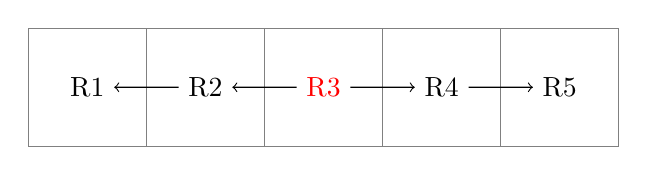
\begin{tikzpicture}[scale = 1.5]
\draw[color = gray] (0,0) grid[xstep = 1cm, ystep = 1cm] (5,1);
\node (R1) at (.5, .5) {R1};
\node (R2) at (1.5,.5) {R2};
\node (R3) [color =  red]  at (2.5,.5) {R3};
\node (R4) at (3.5,.5) {R4};
\node (R5) at (4.5,.5) {R5};
\draw [->] (R3) -- (R2);
\draw [->] (R3) -- (R4);
\draw [->] (R2) -- (R1);
\draw [->] (R4) -- (R5);
\end{tikzpicture}
\end{figure}

Similarly, if we study crime at the city level then somehow we should incorporate the possibility that crime is localized. For example identification of concentration or cluster of greater criminal activity has emerged as a central mechanism to targeting a criminal justice and crime prevention response to crime problem. These clusters of crime are commonly referred to as \textbf{hotpots}: geographic locations of high crime concentration, relative to the distribution of crime across the whole region of interest. 

Both examples implicitly state that geography location and distance matter. In fact, they reflect the importance of the first law of geography. According to Waldo Tobler: \emph{``everything is related to everything else'', but near things are more related than distant things}. This first law is the foundation of the fundamental concepts of \textbf{spatial dependence} and \textbf{spatial autocorrelation}.\index{Tobler's law}

%---------------------------------------------
\subsection{Spatial Dependence}\label{sec:spatial_dependence}\index{Spatial dependence}
%---------------------------------------------

Spatial dependence reflects a situation where values observed at one location or region, say observation $i$, depend on the values of neighboring observations at nearby locations. Formally, we might state

\begin{equation*}
  y_i = f(y_j),\quad i = 1,...,n\;, j\neq i.
\end{equation*}

In words, what happens in region $i$, depends on what happens in region $j$ for all $j\neq i$. Using our previous example, we would like to estimate 

\begin{equation*}
  \begin{aligned}
y_1 & = \beta_{21} y_2 + \beta_{31} y_3 + \beta_{41} y_4 + \beta_{51} y_5 + \epsilon_1 \\
y_2 & = \beta_{12} y_1 + \beta_{32} y_3 + \beta_{42} y_4 + \beta_{52} y_5 + \epsilon_2 \\
y_3 & = \beta_{13} y_1 + \beta_{23} y_2 + \beta_{43} y_4 + \beta_{53} y_5 + \epsilon_3 \\
y_4 & = \beta_{14} y_1 + \beta_{24} y_2 + \beta_{34} y_3 + \beta_{54} y_5 + \epsilon_4 \\
y_5 & = \beta_{15} y_1 + \beta_{25} y_2 + \beta_{35} y_3 + \beta_{45} y_5 + \epsilon_4 
\end{aligned}
\end{equation*}
%
where $\beta_{ji}$ is the effect of pollution of region $j$ on region $i$. However, it is easy to see that  this would be of little practical usefulness, since it would result in a system with many more parameters than observations: we have $n = 5$ observations, but 20 parameters to be estimated, which implies that we do not have sufficient degrees of freedom. Intuitively, once we allow for dependence relation between a set of $n$ observations/locations, there are potentially $n^2-n$ relations that could arise. We subtract $n$ from the potential $n^2$ dependence relations because we rule out dependence of an observation on itself. 

The key point is that, under standard econometric modeling, it is impossible to model spatial dependency. However, as we will see in the next sections, we might be able to incorporate spatial relationships more efficiently using the so-called spatial weight matrix. 

%===========================================
\subsection{Spatial Autocorrelation}\label{sec:Spatial_autocorrelation}\index{Spatial autocorrelation}
%===========================================

Another important concept is \textbf{spatial autocorrelation}. In space, the term autocorrelation refers to the correlation between the value of the variable at two different locations. Other ways of defining the same concept are: (1) correlation between the same attribute at two (or more) different locations, or (2) coincidence of values similarity with location similarity. Essentially, spatial autocorrelation is concerned with establishing whether the presence of a variable in one region in a regional system makes the presence of that variable in neighboring regions more, or less, likely.

The counterpart of spatial autocorrelation (and spatial dependency) is spatial randomness.  Spatial randomness means that we cannot observe any spatial pattern in the data. That is, the value we observe in some spatial unit is equally likely as in any other spatial unit. Spatial randomness is important because it will form the null hypothesis later. If rejected, then there is evidence of spatial structure.  

As an example, Figure \ref{fig:MR} plots the spatial distribution of poverty in the Metropolitan Region, Chile. It can be observed that there is some spatial pattern where communes with similar rate of poverty are clustered. 

\begin{figure}[ht]
  \caption{Spatial Distribution of Poverty in Metropolitan Region, Chile}
    \label{fig:MR}
    \centering
    	\begin{minipage}{.9\linewidth}
\begin{knitrout}
\definecolor{shadecolor}{rgb}{0.969, 0.969, 0.969}\color{fgcolor}

{\centering 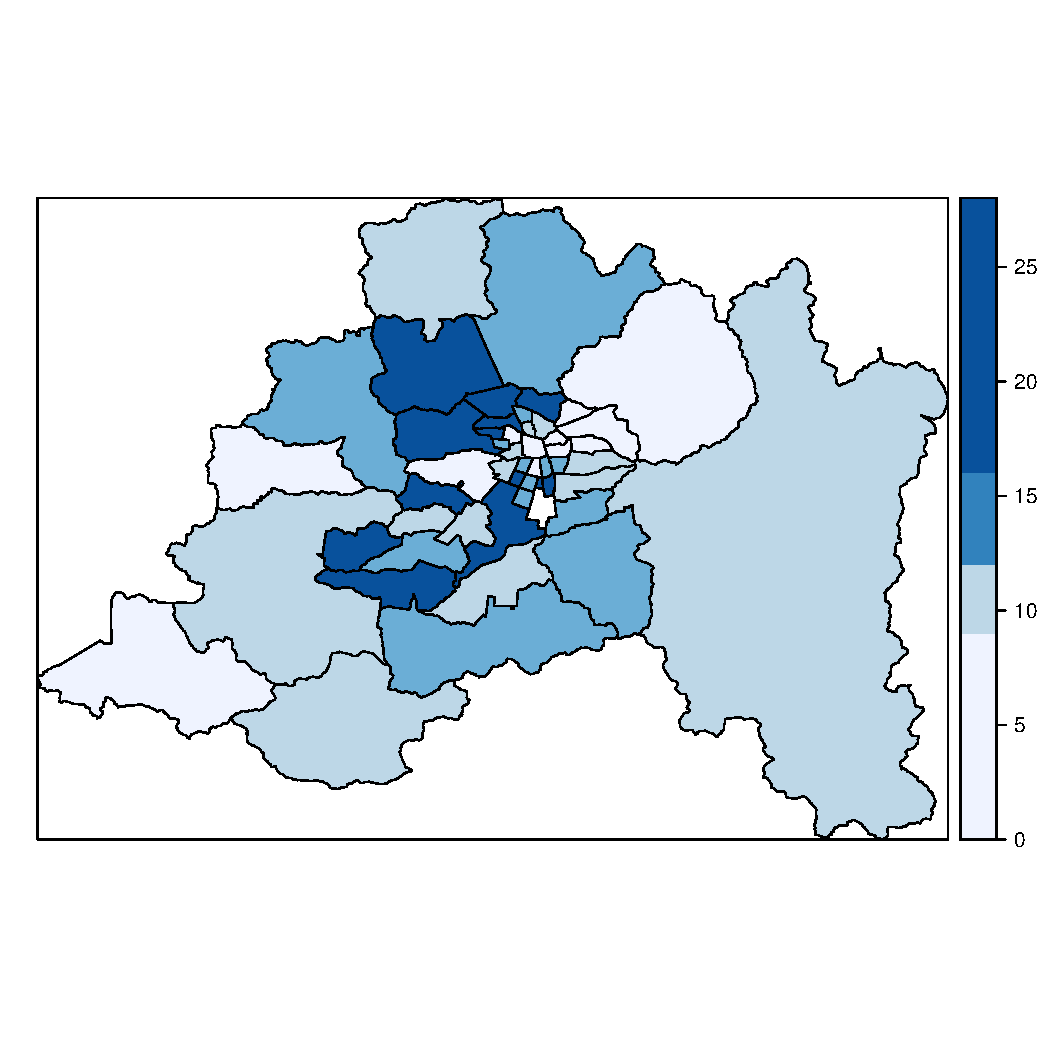
\includegraphics[width=8cm,height=8cm]{figure/MetroRegion-1} 

}


\end{knitrout}
\footnotesize
		\emph{Notes:} This graph shows the spatial distribution of poverty in the Metropolitan Region, Chile. 
	\end{minipage}	
\end{figure}

Formally, the existence of spatial autocorrelation may be expressed by the following moment conditions:

\begin{equation*}
  \cov(y_i, y_j) = \E(y_iy_j) - \E(y_i)\E(y_j)\neq 0\;\;\mbox{for}\;\; i \neq j,
\end{equation*}
%
where $y_i$ and $y_j$ are observations on a random variable at locations $i$ and $j$ in space, and $i,j$ can be points or areal units. Therefore, a nonzero spatial autocorrelation exists between attributes of a feature defined at locations $i$ and $j$ if the covariance between feature attribute values at those points is nonzero. If this covariance is \textbf{positive} (i.e., if data with attribute values above the mean tend to be near other data with values above the mean), then we say there is \textbf{positive spatial autocorrelation}; if the converse is true, then we say there is \textbf{negative spatial autocorrelation}. Figure \ref{fig:Autocorrelation} show an example of positive and negative spatial autocorrelation. 

\begin{figure}[ht]
  \caption{Spatial Autocorrelation}
    \label{fig:Autocorrelation}
    \centering
    	\begin{minipage}{1\linewidth}
\begin{knitrout}
\definecolor{shadecolor}{rgb}{0.969, 0.969, 0.969}\color{fgcolor}

{\centering 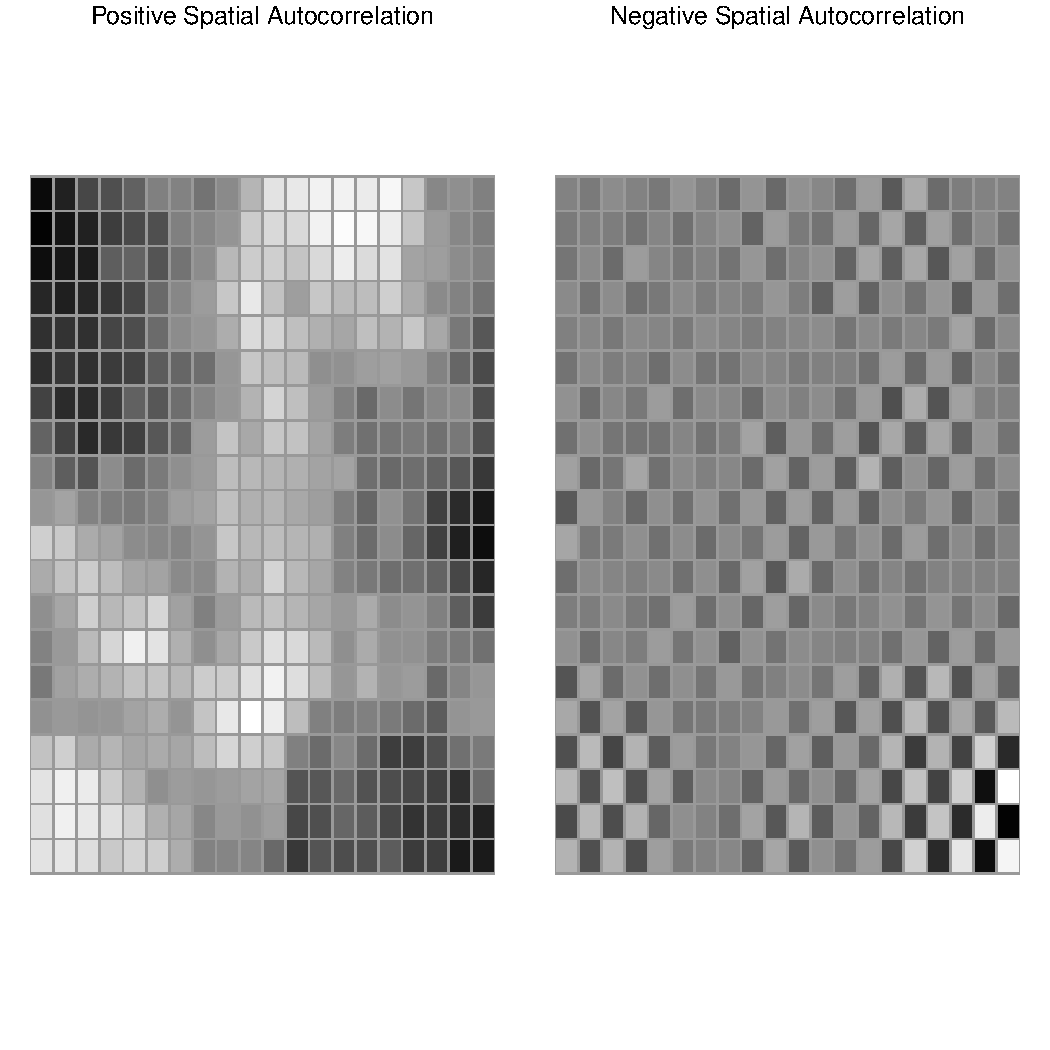
\includegraphics[width=10cm,height=10cm]{figure/Autocorrelation-1} 

}


\end{knitrout}
\footnotesize
		\emph{Notes:} Spatial Autocorrelation among 400 spatial units arranged in an 20-by-20 regular square lattice grid. Different gray-tones refer to different values of the variable ranging from low values (white) to high values (black). The left plot shows positive spatial autocorrelation, whereas right plot shows negative spatial autocorrelation. 
	\end{minipage}	
\end{figure}

Positive autocorrelation is much more common, but negative autocorrelation does exists, for example, in studies of welfare competition or federal grants competitions among local governments \citep{saavedra2000model, boarnet2002federal}, and studies of regional employment \citep{filiztekin2009regional, pavlyuk2011spatial}, the cross-border lottery shopping \citep{garrett2002revenue}, foreign direct investment in OECD countries \citep{garretsen2009fdi} and locations of Turkish manufacturing industry \citep{basdas2009spatial}. In short, we are interested in studying non-random spatial patterns and try to explain this non-randomness. Possible causes of non-randomness are \citep{gibbons2015spatial}:

\begin{enumerate}
	\item Firms may be randomly allocated across space but some characteristics of locations varies across space and influences outcomes. 
	\item Location may have no causal effect on outcomes, but outcomes may be correlated across space because heterogeneous individuals or firms are non-randomly allocated across space. 
	\item Individual or firms may be randomly allocated across  space but they interact so that decisions by one agent affects outcomes of other agents. 
	\item Individuals or firms may be non-randomly allocated across space and the characteristics of others nearby directly influences individual outcomes. 
\end{enumerate}


%********************************
\section{Spatial Weight Matrix}\index{Weight matrix}
%********************************

One of the crucial issues in spatial econometric is the problem of formally incorporating spatial dependence into the model. As we reviewed in Section~\ref{sec:spatial_dependence}, the main problem is that we have more parameter than observations. So, the question is: What would be a good criteria to define closeness in space? Or, in other words, how to determine which other units in the system influence the one under consideration?

The device typically used in spatial analysis to define the concept of closeness in space is the so-called ``spatial weight matrix'', or more simply, $\mW$ matrix. If we assume that there are $n$ spatial objects (regions, cities, countries), then $\mW$ will be a square matrix of dimension $n \times n$. This matrix imposes a structure in terms o what are the neighbors for each location. It assigns weights that measure the intensity of the relationship among pairs of spatial units. Thus, each element $(i,j)$ of $\mW$ -- which we denote by $w_{ij}$ -- expresses the degree of spatial proximity between the pair. This matrix can be represented in the form

\begin{equation*}
\mW = \begin{pmatrix}
        w_{11} & w_{12} & \hdots & w_{1n} \\ 
        w_{21} & w_{22} & \hdots & w_{2n} \\
        \vdots & \vdots & \ddots & \vdots \\
        w_{n1} & w_{n2} & \hdots & w_{nn} 
      \end{pmatrix}
\end{equation*}

Generally, we assume that the diagonal elements of this ``spatial neighbors'' matrix are set to zero: ``regions are not neighbors to themselves''.

A more formal definition of spatial weight matrix is the following:

\begin{definition}[Spatial Weight Matrix]\index{Weight matrix!Definition}\label{def:W}
  Let $n$ be the number of spatial units. The spatial weight matrix, $\mW$, a $n\times n$ positive symmetric and \textbf{non-stochastic} matrix with element $w_{ij}$ at location $i,j$. The values of $w_{ij}$ or the weights for each pair of locations are assigned by some preset rules which define the spatial relations among locations. By convention, $w_{ij} = 0$ for the diagonal elements.
\end{definition}

Non-stochastic means that the researcher takes $\mW$ as known \emph{a priori}, and therefore, all results are conditional upon the specification of $\mW$.

The definition of $\mW$ also requires a rule for $w_{ij}$. In other words, we need to figure out how to assign a real number to $w_{ij}$, for $i\neq j$, representing the strength of the spatial relationship between $i$ and $j$. There are several ways of doing that. But, in general, there are two basic criteria. The first type establishes a relationship based on shared borders or vertices of lattice or irregular polygon data (contiguity). The second type establishes a relationship based on the distance between locations. Generally speaking, contiguity is most appropriate for geographic data expressed as polygons (so-called areal units), whereas distance is suited for point data, although in practice the distinction is not that absolute. 

%==========================================
\subsection{Weights Based on Boundaries}
%==========================================

The availability of polygon or lattice data permits the construction of contiguity-based spatial weight matrices. A typical specification of the contiguity relationship in the spatial weight matrix is

\begin{equation*}
  w_{ij}= 
   \begin{cases}
      1 & \mbox{if $i$ and $j$ are contiguous,} \\ 
      0 & \mbox{if $i$ and $j$ are not contiguous.} 
   \end{cases}
\end{equation*}

In a regular grid, neighbors (contiguity) can be defined in a number of ways. In analogy of the game of chess, rook contiguity, bishop contiguity and queen contiguity are distinguished.

\subsubsection{Rook Contiguity}\index{Weight matrix!Rook contiguity}

In this case, two locations are neighbors if they share at least part of a \textbf{common border or side}. In Figure~\ref{fig:Rook_cont_grid} we have a regular grid with 9 regions: each square represents a region. If for example we want to define the neighbors of region 5 using the rook criteria, then its neighbors will be regions 2, 4, 6 and 8. Those represent the regions filled in red. 

\begin{figure}[h]
\caption{Rook Contiguity}
\label{fig:Rook_cont_grid}
\centering
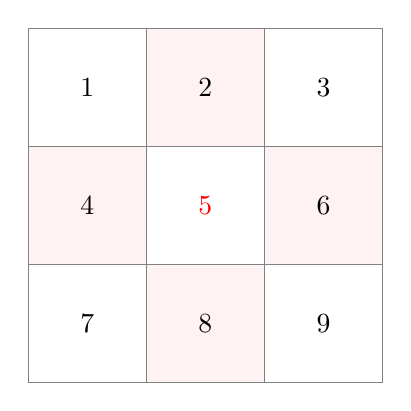
\begin{tikzpicture}[scale = 1.5]
\path [fill=red!5] (1,2) -- (2,2) -- (2,3) -- (1,3);
\path [fill=red!5] (1,0) -- (2,0) -- (2,1) -- (1,1);
\path [fill=red!5] (0,1) -- (1,1) -- (1,2) -- (0,2);
\path [fill=red!5] (2,1) -- (3,1) -- (3,2) -- (2,2);
\draw[color = gray] (0,0) grid[xstep = 1cm, ystep = 1cm] (3,3); % grid of 3 times 3
\node at (.5, 2.5) {1};
\node at (1.5, 2.5) {2};
\node at (2.5, 2.5) {3};
\node at (.5, 1.5) {4};
\node [color =  red] at (1.5,1.5) {5} ;
\node at (2.5,1.5) {6};
\node at (.5, .5) {7};
\node at (1.5,.5) {8};
\node at (2.5,.5) {9};
\end{tikzpicture}
\end{figure}

If we continue with this reasoning, then the $9\times 9$ $\mW$ matrix will be:

\begin{equation}
  \mW = 
  \begin{pmatrix}
     0 & 1 & 0 & 1 & 0 & 0 & 0 & 0 & 0 \\
     1 & 0 & 1 & 0 & 1 & 0 & 0 & 0 & 0 \\
     0 & 1 & 0 & 0 & 0 & 1 & 0 & 0 & 0 \\
     1 & 0 & 0 & 0 & 1 & 0 & 1 & 0 & 0 \\
     0 & 1 & 0 & 1 & 0 & 1 & 0 & 1 & 0 \\
     0 & 0 & 1 & 0 & 1 & 0 & 0 & 0 & 1 \\
     0 & 0 & 0 & 1 & 0 & 0 & 0 & 1 & 0 \\
     0 & 0 & 0 & 0 & 1 & 0 & 1 & 0 & 1 \\
     0 & 0 & 0 & 0 & 0 & 1 & 0 & 1 & 0 \\
  \end{pmatrix}
\end{equation}

\subsubsection{Bishop Contiguity}\index{Weight matrix!Bishop contiguity}

In bishop contiguity (\textbf{which is seldom used in practice}), region $i$'s neighbors are located at its corners. Figure~\ref{fig:Bishop_cont_grid} shows the neighbors of region 5 under this scheme. The neighbors are regions 1, 3, 7 and 9. Note that regions in the interior will have more neighbors than those in the periphery. 


\begin{figure}[h]
\caption{Bishop Contiguity}
\label{fig:Bishop_cont_grid}
\centering
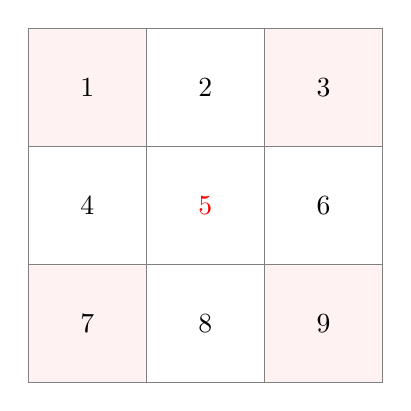
\begin{tikzpicture}[scale = 1.5]
\path [fill=red!5] (0,2) -- (1,2) -- (1,3) -- (0,3);
\path [fill=red!5] (0,0) -- (1,0) -- (1,1) -- (0,1);
\path [fill=red!5] (2,2) -- (3,2) -- (3,3) -- (2,3);
\path [fill=red!5] (2,0) -- (3,0) -- (3,1) -- (2,1);
\draw[color = gray] (0,0) grid[xstep = 1cm, ystep = 1cm] (3,3); % grid of 3 times 3
\node at (.5, 2.5) {1};
\node at (1.5, 2.5) {2};
\node at (2.5, 2.5) {3};
\node at (.5, 1.5) {4};
\node [color =  red] at (1.5,1.5) {5} ;
\node at (2.5,1.5) {6};
\node at (.5, .5) {7};
\node at (1.5,.5) {8};
\node at (2.5,.5) {9};
\end{tikzpicture}
\end{figure}

The resulting $\mW$ matrix will be:

\begin{equation*}
\mW = 
  \begin{pmatrix}
     0 & 0 & 0 & 0 & 1 & 0 & 0 & 0 & 0 \\
     0 & 0 & 0 & 1 & 0 & 1 & 0 & 0 & 0 \\
     0 & 0 & 0 & 0 & 1 & 0 & 0 & 0 & 0 \\
     0 & 1 & 0 & 0 & 0 & 0 & 0 & 1 & 0 \\
     1 & 0 & 1 & 0 & 0 & 0 & 1 & 0 & 1 \\
     0 & 1 & 0 & 0 & 0 & 0 & 0 & 1 & 0 \\
     0 & 0 & 0 & 0 & 1 & 0 & 0 & 0 & 0 \\
     0 & 0 & 0 & 1 & 0 & 1 & 0 & 0 & 0 \\
     0 & 0 & 0 & 0 & 1 & 0 & 0 & 0 & 0 \\
  \end{pmatrix}
\end{equation*}

This criteria is seldom used in practice. 

\subsubsection{Queen Contiguity}\index{Weight matrix!Queen contiguity}

In queen contiguity, any region that touches the boundary of region $i$, whether on a side or a single point, is considered neighbor. Under this criteria, the neighbors of 5 will be regions: 1, 2, 3, 4, 6, 7, 8 and 9.

\begin{figure}[h]
\caption{Queen Contiguity}
\label{fig:Queen_cont_grid}
\centering
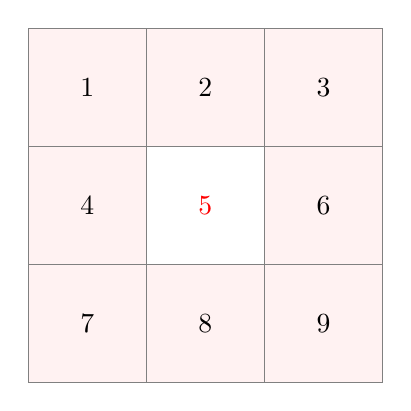
\begin{tikzpicture}[scale = 1.5]
\path [fill=red!5] (0,2) -- (1,2) -- (1,3) -- (0,3);
\path [fill=red!5] (0,0) -- (1,0) -- (1,1) -- (0,1);
\path [fill=red!5] (2,2) -- (3,2) -- (3,3) -- (2,3);
\path [fill=red!5] (2,0) -- (3,0) -- (3,1) -- (2,1);
\path [fill=red!5] (1,2) -- (2,2) -- (2,3) -- (1,3);
\path [fill=red!5] (1,0) -- (2,0) -- (2,1) -- (1,1);
\path [fill=red!5] (0,1) -- (1,1) -- (1,2) -- (0,2);
\path [fill=red!5] (2,1) -- (3,1) -- (3,2) -- (2,2);
\draw[color = gray] (0,0) grid[xstep = 1cm, ystep = 1cm] (3,3); % grid of 3 times 3
\node at (.5, 2.5) {1};
\node at (1.5, 2.5) {2};
\node at (2.5, 2.5) {3};
\node at (.5, 1.5) {4};
\node [color =  red] at (1.5,1.5) {5} ;
\node at (2.5,1.5) {6};
\node at (.5, .5) {7};
\node at (1.5,.5) {8};
\node at (2.5,.5) {9};
\end{tikzpicture}
\end{figure}


%=========================================
\subsection{Weights Based on Distance}\index{Weight matrix!Based on distance}
%=========================================

Weights may also be defined as a function of the distance between region $i$ and $j$, $d_{ij}$. This distance is usually computed as the distance between their centroids, but it may of course be between other relevant points for each spatial units, such as the capital -- or largest city-- or each region. Unlike the weights based on contiguity, matrices based on distances only need the coordinates of the points.

There are several ways of computing the distance between two spatial units. Let $x_i$ and $x_j$ be the longitude; and $y_i$ and $y_j$ the latitude coordinates for region $i$ and $j$, respectively. The most general concept of distance is the Minkowski metric:

\begin{equation*}
  d_{ij}^p = \left(\left|x_i - x_j\right|^p + \left|y_i - y_j\right|^p\right),
\end{equation*}
%
for two points $i$ and $j$, with respective coordinates $(x_i, y_i)$ and $(x_j, y_j)$, and with $p$ as the parameter. The most familiar special case is the Euclidean or straight line distance with $p = 2$:

\begin{equation*}
  d_{ij}^e = \sqrt{(x_i - x_j)^2 + (y_i - y_j)^2}.
\end{equation*}

Another employed metric is the Manhattan block distance. This measure only considers movement along the east-west and north-south directions, i.e., by straight angles. This yield a distance measure where $p = 1$:

\begin{equation*}
   d_{ij}^m = \left|x_i - x_j\right| + \left|y_i - y_j\right|.
\end{equation*}

All three measures presented above are useful if we consider the earth as a plane. For example, the Euclidean distance is the length of a straight line on a map, and is not necessarily the shortest distance if you take into account the curvature of the earth. The great circle distance take into account the curvature of Earth. Ships and aircraft usually follow the great circle geometry to minimize the distance and save time and money.  In particular, the great circle distance is computed as:

\begin{equation*}
d_{ij}^{cd} = r \times \arccos^{-1}\left[\cos|x_i - x_j| \cos y_i \cos y_j + \sin y_i \sin y_j \right]
\end{equation*}
%
where $r$ is the Earth's radius. The arc distance is obtained in miles with $r = 3959$ and in kilometers with $r = 6371$.

%=================================
\subsubsection{Inverse Distance}\label{sec:inverse_distance}
%=================================

Now we have to transform the information about the distances among spatial points into a weight scheme. The idea is that $w_{ijt}\to 0$ as $d_{ij}\to \infty$. In other words, the closer is $j$ to $i$, the larger $w_{ij}$ should be to conform to Tobler's first law. 

In the inverse distance weighting scheme, the weights are inversely related to separation distance as shown below:

\begin{equation*}
  w_{ij} =
  \begin{cases}
  \frac{1}{d_{ij}^{\alpha}} & \mbox{if} \;\;i \neq j \\
  0 & \mbox{if}\;\; i = j,
  \end{cases}
\end{equation*}
%
where the exponent $\alpha$ is a parameter that is usually set by the researcher. In practice, the parameters are seldom estimated, but typically set to $\alpha = 1$ or $\alpha = 2$. Therefore, the weights are given by  the reciprocal of the distance: the larger the distance between to spatial units, the lowest the spatial weight or the spatial connection. Finally, by convention, the diagonal elements of the spatial weights are set to zero and not computed. Plugging in a value of $d_{ii} = 0$ would yield division by zero for inverse distance weights. 

\subsubsection{Negative Exponential Model}

Here the weights decline exponentially with separation distance

\begin{equation*}
  w_{ij} = \exp\left(-\frac{d_{ij}}{\alpha}\right),
\end{equation*}
%
where $\alpha$ is a parameter that is commonly chosen by researcher. Since the weights are given by the exponential of the negative distance, the greater the distance between $i$ and $j$, the lower $w_{ij}$.

Both the inverse distance and the negative exponential distance depend not only on the parameter value and functional form, but also on the metric used for distance. Since the weights are inversely related to distance, larger values for the latter will yield small values for the former, and vice versa. This may be a problem in practice when the distances are so large that the corresponding inverse distance weights become close to zero, possible resulting in a zero spatial weight matrix. In addition, a potential problem may occur when the distance metric is such that distances take on values less than one, which is typically a not a desired result \citep{anselin2014modern}. 

\subsubsection{$k$-nearest Neighbors}

An alternative type of spatial weights that avoids the problem of isolates is to select the $k$-nearest neighbors. In contrast to the distance band, this is not a symmetric relation. However, a potential problem with this type of neighbors is the occurrence of ties, i.e., when more than one location $j$ has the same distance from $i$. A number of solutions exist to break the tie, from randomly selecting one the $k$-th order neighbors, to including all of them. 

\subsubsection{Threshold Distance (Distance Band Weights)}

In contrast to the $k$-nearest neighbors method, the threshold distance specifies that an region $i$ is neighbor of $j$ if the distance between them is less than a specified maximum distance:


\begin{equation*}
  w_{ij}= 
   \begin{cases}
      1 & \mbox{if}\;\; 0\leq d_{ij} \leq d_{max} \\ 
      0 & \mbox{if}\;\; d_{ij} > d_{max}.
   \end{cases}
\end{equation*}


To avoid isolates that would result from too stringent a critical distance, the distance must be chosen such that each location has at least one neighbor. Such a distance conforms to a max-min criterion, i.e., it is the largest of the nearest neighbor distances.

Finally, it is important to note that a weights matrix obtained from a distance band is always symmetric, since distance is a symmetric relation. 

%============================================
\subsection{Row-Standardized Weights Matrix}\index{Weight matrix!Row-standardization}
%============================================

In practice, the spatial weights are seldom used in their binary (or distance) form, but subject to a transformation or standardization. In particular, we would like to compute weighted averages in which more weight is placed on nearby observations than on distant observations. To do so, we can define a row-standardized weight matrix $\mW^s$, whose element $w_{ij}^s$ is given by:

\begin{equation*}
w_{ij}^s = \frac{w_{ij}}{\sum_j w_{ij}}.
\end{equation*}

This ensures that all weights are between 0 and 1 and facilities the interpretation of operation with the weights matrix as an averaging of neighboring values as we will see below. The row-standardized weights matrix also ensures that the spatial parameter in many spatial stochastic processes are comparable between models  \citep{AnselinBera1998}.

Another important feature is that, under row-standardization, the element of each row sum to unity and the sum of all weights, $S_0 = \sum_i\sum_j w_{ij} = n$, the total number of observations. This is a nice interpretation that we will explore later.

Another important issue is about symmetry. An important characteristic of symmetric matrix is that all its characteristics roots are real. However, \textbf{after the row standardization the matrices are no longer symmetric.} 

The row-standardized matrix is also known in the literature as the row-stochastic matrix:


\begin{definition}[Row-stochastic Matrix]
	A real $n\times n$ matrix $\mA$ is called \textbf{Markov} matrix, or \textbf{row-stochastic matrix} if 
		\begin{enumerate}
			\item $a_{ij} \geq 0$ for $1\leq i, j \leq n$;
			\item $\sum_{j=1}^n a_{ij} = 1$ for $1\leq i \leq n$
		\end{enumerate}
\end{definition}


An important characteristic of the row-stochastic matrix is related to its eigen values:


\begin{theorem}[Eigenvalues of row-stochastic Matrix]\label{teo:eigen_values}
	Every eigenvalue $\omega_i$ of a row-stochastic Matrix satisfies $\left|\vomega\right|\leq 1$
\end{theorem}

Therefore, the eigenvalues of the row-stochastic (i.e., row-normalized, row standardized or Markov) neighborhood matrix $\mW^s$ are in the range $\left[-1, +1\right]$.

Finally, the behavior of $\mW^s$ is important for asymptotic properties of estimators and test statistics \citep[][pp. 244]{AnselinBera1998}. In particular, the $\mW$ matrix should be also exogenous, unless endogeneity is considered explicitly in the model specification. 

%============================================
\subsection{Spatial Lagged Variables}\label{sec:spatial_lag_var}\index{Weight matrix!Spatial lag}
%============================================

Now that we have discussed the spatial weight matrix, we can create the so-called \textbf{spatially lagged variables} or \textbf{spatial lag operator}. The spatial lag operator takes the form $\vy_L = \mW\vy$ with dimension $n \times 1$, where each element is given by $\vy_{Li} = \sum_{j}w_{ij}y_j$, i.e., a weighted average of the $\vy$ values in the neighbor of $i$.

For example:

\begin{equation*}
  \mW\vy =    \begin{pmatrix}
     0 & 1 & 0 \\
     1 & 0 & 1 \\
     0 & 1 & 0
  \end{pmatrix}
  \begin{pmatrix}
     10 \\
     50 \\
     30
  \end{pmatrix} =
  \begin{pmatrix}
     50 \\
     10 + 30 \\
     50
  \end{pmatrix}.
\end{equation*}

Using a row-standardized weight matrix:

\begin{equation*}
  \mW\vy =    \begin{pmatrix}
     0 & 1 & 0 \\
     0.5 & 0 & 0.5 \\
     0 & 1 & 0
  \end{pmatrix}
  \begin{pmatrix}
     10 \\
     50 \\
     30
  \end{pmatrix} =
  \begin{pmatrix}
     50 \\
     5 + 15 \\
     50
  \end{pmatrix}.
\end{equation*}

As a result, for spatial unit $i$, the spatial lag of $y_i$, referred as $\vy_{Li}$ ( the variable $Wy$ observed for location $i$) is:

\begin{equation*}
  \vy_{Li} = w_{i, 1}y_i + w_{i, 2}y_2 + ... + w_{i, n}y_n, 
\end{equation*}
%
or,

\begin{equation*}
  \vy_{Li} = \sum_{j = 1}^nw_{i,j}y_j,
\end{equation*}
%
where the weights $w_{ij}$ consists of the elements of the $i$th row of the matrix $\mW$, matched up with the corresponding elements of the vector $\vy$. In other words, this is a weighted sum of the values observed at neighboring locations, since the non-neighbors are not included. 

\begin{remark}
As stated by \citet[][p. 23-24]{anselin1988spatial}, standardization must be done with caution.\footnote{See also \citet[][p. 12]{elhorst2014spatial} and references therein.} For example, when the weights are based on an inverse distance function (or similar concept of distance decay), which has a meaningful economic interpretation, scaling the rows so that the weights sum to one may result in a loss of that interpretation. Can you give an example?
\end{remark}


%============================================
\subsection{Higher Order Spatial}\label{sec:HSO}\index{Weight matrix!Higher order}
%============================================

So far we have learned how to define the geographical space by matrix $\mW$. However, an interesting question is how to define higher-order neighbors. For example, we may be interested in defining the neighbors of the neighbors of a spatial unit. Or even we might be interested in the neighbors of neighbors of neighbors of spatial unit $i$. To discuss this interesting case we need to define \textbf{higher-order spatial weight matrices}. 

We define the higher-order spatial weight matrix $l$ as $\mW^l$. So, for example the spatial weight of order $l=2$ is given by $\mW^2 = \mW\mW$, spatial weight matrix of order $l = 3$ is given by $\mW^3 = \mW\mW\mW$, and so on. What is the meaning of the element $w_{ij}$ in this case? For spatial weights of order 2, the element $w_{ij}$ of the weight matrix is 1 if polygon $j$ is adjacent to the first order neighbors of polygon $i$ and is 0 otherwise. Thus, for spatial neighbor weights of order $n$, the element $w_{ij}$ of the weight matrix $\mW$ is 1 if polygon $j$ is adjacent to the neighbors of order $n-1$ of polygon $i$, and is 0 otherwise. 

To illustrate these points, consider the following spatial structure for our example in Section \ref{sec:why_se}:

\begin{equation}\label{eq:W5x5}
\mW = \begin{pmatrix}
      0 & 1 & 0 & 0 & 0 \\
      1 & 0 & 1 & 0 & 0 \\
      0 & 1 & 0 & 1 & 0 \\
      0 & 0 & 1 & 0 & 1 \\
      0 & 0 & 0 & 1 & 0
      \end{pmatrix}.
\end{equation}

Then $\mW^2 = \mW\mW$ based on the $5\times 5$ first-order contiguity matrix $\mW$ from (\ref{eq:W5x5}) is:

\begin{equation}
\mW^2 = \begin{pmatrix}\label{eq:W25x5}
      1 & 0 & 1 & 0 & 0 \\
      0 & 2 & 0 & 1 & 0 \\
      1 & 0 & 2 & 0 & 1 \\
      0 & 1 & 0 & 2 & 0 \\
      0 & 0 & 1 & 0 & 1
      \end{pmatrix}
\end{equation}

Note that for region $R1$, the second-order neighbors are regions $R1$ and $R3$. That is, region $R1$ is a second-order neighbor to itself as well as to region $R3$, which is a neighbor to the neighboring region $R2$. 

Now consider R2. The first panel of Figure \ref{fig:example_hon} shows the first-order neighbors of $R2$ given by the spatial weight matrix in (\ref{eq:W5x5}): the first-order neighbors are R1 and R3. Panel B considers the second-order neighbors of $R2$: the second-order neighbors are $R2$ itself and $R4$. To understand this, note that there is a feedback effect from the first impact from $R2$ coming from $R1$ and $R3$ (first-order neighbors of $R2$). This explains why the element $w^2_{22} = 2$. Moreover, there is an indirect effect coming from $R4$ through $R3$ that finally impacts $R2$.  This represents the value of 1 for the element $w^2_{24}$.

Similarly, for region $R3$, the second-order neighbors are regions $R1$ (which is a neighbor to the neighboring region $R2$), $R3$ (a second-order neighbor to itself), and $R5$ (which is a neighbor to the neighboring region $R4$). 

\begin{figure}[ht]
\caption{Higher-Order Neighbors}
\label{fig:example_hon}
\centering
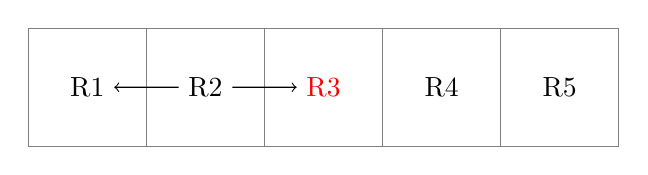
\begin{tikzpicture}[scale = 1.5]
\draw[color = gray] (0,0) grid[xstep = 1cm, ystep = 1cm] (5,1);
\node (R1) at (.5, .5) {R1};
\node (R2) at (1.5,.5) {R2};
\node (R3) [color =  red]  at (2.5,.5) {R3};
\node (R4) at (3.5,.5) {R4};
\node (R5) at (4.5,.5) {R5};
\draw [->] (R2) -- (R1);
\draw [->] (R2) -- (R3);
\end{tikzpicture}
\\
\vspace{1cm}
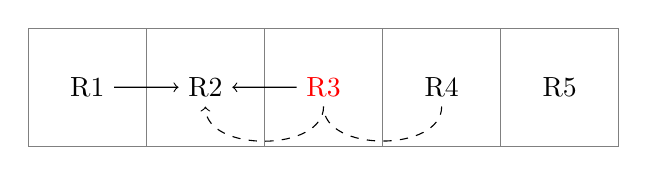
\begin{tikzpicture}[scale = 1.5]
\draw[color = gray] (0,0) grid[xstep = 1cm, ystep = 1cm] (5,1);
\node (R1) at (.5, .5) {R1};
\node (R2) at (1.5,.5) {R2};
\node (R3) [color =  red]  at (2.5,.5) {R3};
\node (R4) at (3.5,.5) {R4};
\node (R5) at (4.5,.5) {R5};
\draw [->] (R1) -- (R2);
\draw [->] (R3) -- (R2);
\draw [->, dashed] (R4) to[out= 270,in=270] (R3) to[out=270,in=270] (R2);
\end{tikzpicture}
\end{figure}

Similarly, the third-order neighbors are: 


\begin{equation*}
\mW^3 = \begin{pmatrix}
      0 & 2 & 0 & 1 & 0 \\
      2 & 0 & 3 & 0 & 1 \\
      0 & 3 & 0 & 3 & 0 \\
      1 & 0 & 3 & 0 & 2 \\
      0 & 1 & 0 & 2 & 1
      \end{pmatrix}
\end{equation*}

Could you explain the elements of this matrix?


%============================================
\section{Examples of Weight Matrices in R}
%============================================

Creating spatial weight matrices by hand is tedious (and in some cases almost impossible). However, there exists several statistical software that allow us to create them in a very simply fashion.  First, we need the \textbf{shape file}, which has geographical information.  The shapefile format is a digital vector storage for storing geometric location and associated attribute information. Nowadays it is possible to read and write geographical datasets using the shapefile format with a wide variety of software.

The shapefile format is simple because it can store the primate geometric data types of points, lines and polygons. Shapes (points/lines/polygons) together with data attributes can create infinitely many representations about geographic data. The three mandatory files have filename extensions \texttt{.shp, .shx}, and \texttt{.dbf}. The actual shapefile relates specifically to the \texttt{.shp} file, but alone is incomplete for distribution as the other supporting files are required. The characteristics of each file is the following:

\begin{itemize}
  \item \texttt{.shp}: shape format; the feature geometry itself,
  \item \texttt{.shx}: shape index format; a positional index of the feature geometry to allow seeking forwards and backwards quickly,
  \item \texttt{.dbf}: attribute format; columnar attributes for each shape, in \texttt{dBase} IV format. 
\end{itemize}

For simplicity in showing how to create neighbor objects in \proglang{R}, we work on the map consisting of the communes of the Metropolitan Region in Chile. 

We first need to load the Metropolitan Region shape file in \proglang{R}. To do so, we will use the \pkg{maptools} package \citep{maptoolsP}, which allows us reading and handling spatial objects. 

\begin{knitrout}
\definecolor{shadecolor}{rgb}{0.969, 0.969, 0.969}\color{fgcolor}\begin{kframe}
\begin{alltt}
\hlcom{#Load package}
\hlkwd{library}\hlstd{(}\hlstr{"maptools"}\hlstd{)}
\end{alltt}
\end{kframe}
\end{knitrout}

If the shape file \code{mr\_chile.shp} is in the same working directory, then we can load it into \proglang{R} using the command \code{readShapeSpatial}:

\begin{knitrout}
\definecolor{shadecolor}{rgb}{0.969, 0.969, 0.969}\color{fgcolor}\begin{kframe}
\begin{alltt}
\hlcom{# Read shape file}
\hlstd{mr} \hlkwb{<-} \hlkwd{readShapeSpatial}\hlstd{(}\hlstr{"mr_chile.shp"}\hlstd{)}
\hlkwd{class}\hlstd{(mr)}
\end{alltt}
\begin{verbatim}
## [1] "SpatialPolygonsDataFrame"
## attr(,"package")
## [1] "sp"
\end{verbatim}
\end{kframe}
\end{knitrout}

The function \texttt{readShapeSpatial} reads data from the shapefile into a \code{Spatial} object of class ``\code{sp}''. The function \code{names} give us the name of the variables in the \texttt{.dbf} file associated with the shape file. 

\begin{knitrout}
\definecolor{shadecolor}{rgb}{0.969, 0.969, 0.969}\color{fgcolor}\begin{kframe}
\begin{alltt}
\hlcom{# Names of the variables in .dbf}
\hlkwd{names}\hlstd{(mr)}
\end{alltt}
\begin{verbatim}
##  [1] "ID"         "NAME"       "NAME2"      "URB_POP"    "RUR_POP"   
##  [6] "MALE_POP"   "TOT_POP"    "FEM_POP"    "N_PARKS"    "N_PLAZA"   
## [11] "CONS_HOUSE" "M2_CONS_HA" "GREEN_AREA" "AREA"       "POVERTY"   
## [16] "PER_CONTR_" "PER_HON_SA" "PER_PLANT_" "NURSES"     "DOCTORS"   
## [21] "CONSULT_RU" "CONSULT_UR" "POSTAS"     "ESTAB_MUN_" "PSU_MUN_PR"
## [26] "PSU_PART_P" "PSU_SUB_PR" "STUDENT_SU" "STUDENT_PA" "STUDENT_MU"
\end{verbatim}
\end{kframe}
\end{knitrout}

We can plot the shapefile using the generic function \code{plot} in the following way

\begin{knitrout}
\definecolor{shadecolor}{rgb}{0.969, 0.969, 0.969}\color{fgcolor}\begin{kframe}
\begin{alltt}
\hlcom{# Plot shapefile}
\hlkwd{plot}\hlstd{(mr,} \hlkwc{main} \hlstd{=} \hlstr{"Metropolitan Region-Chile"}\hlstd{,} \hlkwc{axes} \hlstd{=}  \hlnum{TRUE}\hlstd{)}
\end{alltt}
\end{kframe}
\end{knitrout}

The metropolitan region with the 52 communes is shown in Figure \ref{fig:plot_mr}.

\begin{figure}[h]
  \caption{Plotting a Map in R}
    \label{fig:plot_mr}
\begin{knitrout}
\definecolor{shadecolor}{rgb}{0.969, 0.969, 0.969}\color{fgcolor}

{\centering 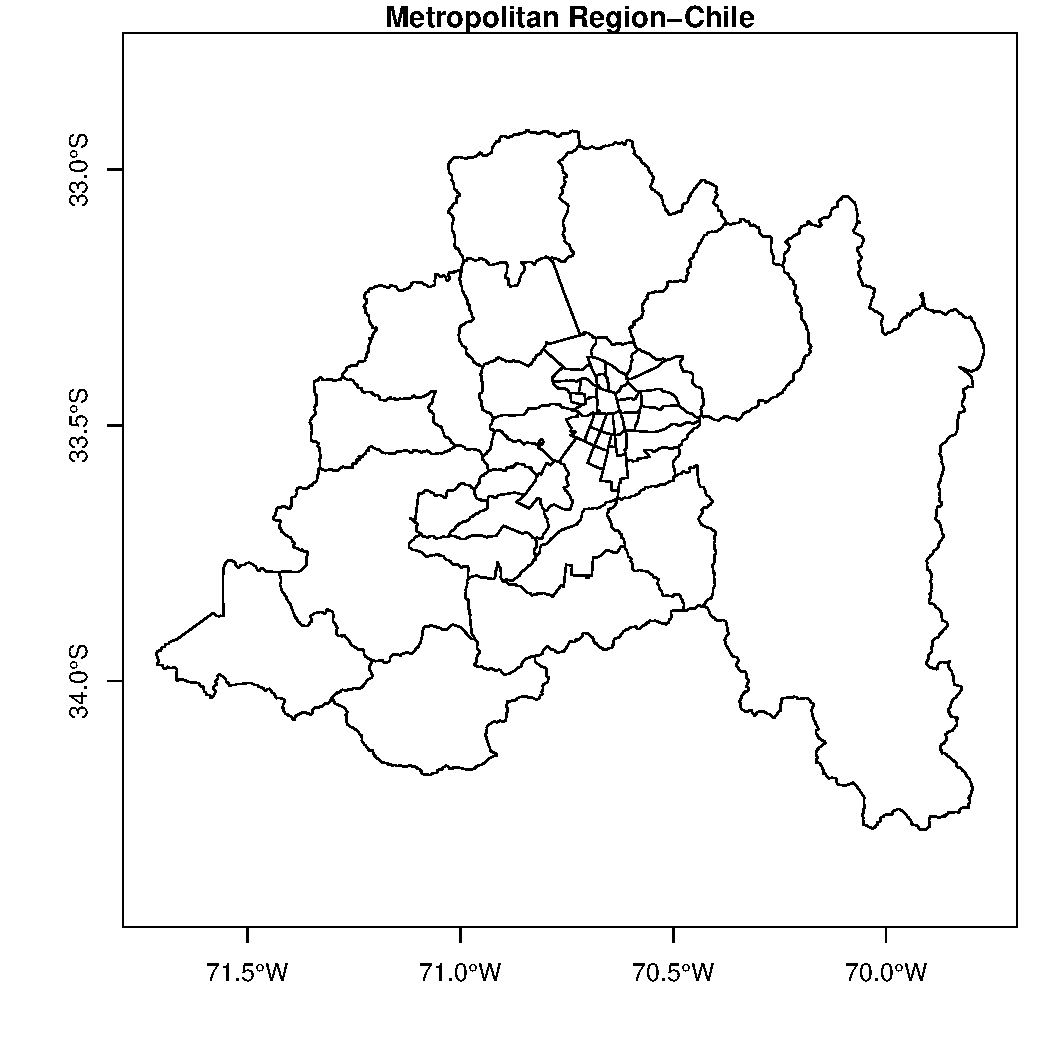
\includegraphics[width=8cm,height=8cm]{figure/plot_mr-1} 

}


\end{knitrout}
\end{figure}

%===============================================
\subsection{Creating Contiguity Neighbors}
%===============================================

To create spatial weight matrices we need the \pkg{spdep} package \citep{bivand2013computing}. After installing it, we load the package

\begin{knitrout}
\definecolor{shadecolor}{rgb}{0.969, 0.969, 0.969}\color{fgcolor}\begin{kframe}
\begin{alltt}
\hlcom{#Load package}
\hlkwd{library}\hlstd{(}\hlstr{"spdep"}\hlstd{)}
\end{alltt}
\end{kframe}
\end{knitrout}

In the \pkg{spdep} package, neighbor relationships between $n$ observations are represented by an object of class ``\code{nb}''. This object is a list of length $n$ with the index numbers of neighbors of each component recorded as an integer vector. If any observation has no neighbors, the component contains an integer zero. 


The function \code{poly2nb} is used in order to construct weight matrices based on \textbf{contiguity}. Specifically, it creates a ``neighbors list'' based on regions with contiguous boundaries of class ``\code{nb}''. Check out \code{help(polynb)} to see all the details and options. 

First, we create a neighbor list based on the `Queen' criteria for the communes of the Metropolitan Region\index{Weight matrix!poly2nb function}:

\begin{knitrout}
\definecolor{shadecolor}{rgb}{0.969, 0.969, 0.969}\color{fgcolor}\begin{kframe}
\begin{alltt}
\hlcom{# Create queen W}
\hlstd{queen.w} \hlkwb{<-} \hlkwd{poly2nb}\hlstd{(mr,} \hlkwc{row.names} \hlstd{= mr}\hlopt{$}\hlstd{NAME,} \hlkwc{queen} \hlstd{=}  \hlnum{TRUE}\hlstd{)}
\end{alltt}
\end{kframe}
\end{knitrout}

Since we have an \code{nb} object to examine, we can present the standard methods for these objects. There are \code{print}, \code{summary}, \code{plot}, and other methods. The characteristics of the weights are obtained with the usual \code{summary} command:

\begin{knitrout}
\definecolor{shadecolor}{rgb}{0.969, 0.969, 0.969}\color{fgcolor}\begin{kframe}
\begin{alltt}
\hlcom{# Summary of W}
\hlkwd{summary}\hlstd{(queen.w)}
\end{alltt}
\begin{verbatim}
## Neighbour list object:
## Number of regions: 52 
## Number of nonzero links: 292 
## Percentage nonzero weights: 10.79882 
## Average number of links: 5.615385 
## Link number distribution:
## 
##  2  3  4  5  6  7  8  9 10 12 
##  3  2  7 15 10 10  2  1  1  1 
## 3 least connected regions:
## Tiltil San Pedro Maria Pinto with 2 links
## 1 most connected region:
## San Bernardo with 12 links
\end{verbatim}
\end{kframe}
\end{knitrout}

The output presents important information about the neighbors: it shows the number of regions, which corresponds to 52 in this example; the number of nonzero links; the percentage of nonzero weights; the average number of links, and so on. 

The commune of San Bernardo is most connected region with 12 neighbors under the queen scheme. The least connected regions are Tiltil, San Pedro, and Maria Pinto with 2 neighbors each of them. The output also shows the distribution of neighbors.  For example, 7 out of 52 regions has 4 neighbors and only 2 communes has 8 neighbors.  

To transform the \code{list} into an actual matrix $\mW$, we can use the function \code{nb2listw}\index{Weight matrix!nb2listw function}:


\begin{knitrout}
\definecolor{shadecolor}{rgb}{0.969, 0.969, 0.969}\color{fgcolor}\begin{kframe}
\begin{alltt}
\hlcom{# From list to matrix}
\hlstd{queen.wl} \hlkwb{<-} \hlkwd{nb2listw}\hlstd{(queen.w,} \hlkwc{style} \hlstd{=} \hlstr{"W"}\hlstd{)}
\hlkwd{summary}\hlstd{(queen.wl)}
\end{alltt}
\begin{verbatim}
## Characteristics of weights list object:
## Neighbour list object:
## Number of regions: 52 
## Number of nonzero links: 292 
## Percentage nonzero weights: 10.79882 
## Average number of links: 5.615385 
## Link number distribution:
## 
##  2  3  4  5  6  7  8  9 10 12 
##  3  2  7 15 10 10  2  1  1  1 
## 3 least connected regions:
## Tiltil San Pedro Maria Pinto with 2 links
## 1 most connected region:
## San Bernardo with 12 links
## 
## Weights style: W 
## Weights constants summary:
##    n   nn S0       S1      S2
## W 52 2704 52 19.76751 216.466
\end{verbatim}
\end{kframe}
\end{knitrout}

An important argument of the function is \code{style}. This argument indicates what type of matrix to create. For example, \code{style = "W"} creates a row-standardize matrix so that $w^s_{ij} = w_{ij}/ \sum_j w_{ij}$. After normalization, each row of $\mW^s$ will sum to 1. \code{"B"} is the basic binary coding; and \code{"C"} is globally standardize, that is, $w^s_{ij} = w_{ij} \cdot (n/ \sum_{i}\sum_j w_{ij})$. If \code{style = "U"}, then $w^s_{ij} = w_{ij}/ \sum_i\sum_j w_{ij}$. In a \code{minmax} matrix, the $(i,j)$th element of $\mW^s$  becomes $w^s_{ij} = w_{ij} / \min\left\lbrace \max_i(\tau_i), \max_i(c_i)\right\rbrace$, with $\max_i(\tau_i)$ being the largest row sum of $\mW$ and $\max_i(c_i)$ being the largest column sum of $\mW$ \citep{kelejian2010specification}. Finally, \code{"S"} is the variance-stabilizing coding scheme where $w^s_{ij} = w_{ij}/ \sqrt{\sum_j w_{ij} ^2}$ \citep{tiefelsdorf1999variance}. 

Furthermore, the \code{summary} function reports constants used in the inference for global spatial autocorrelation statistics, which we will discuss later. 

We can also see the attributes of the object using the function \code{attributes}:


\begin{knitrout}
\definecolor{shadecolor}{rgb}{0.969, 0.969, 0.969}\color{fgcolor}\begin{kframe}
\begin{alltt}
\hlcom{# Attributes of wlist}
\hlkwd{attributes}\hlstd{(queen.w)}
\end{alltt}
\begin{verbatim}
## $class
## [1] "nb"
## 
## $region.id
##  [1] Santiago            Cerillos            Cerro Navia        
##  [4] Conchali            El Bosque           Estacion Central   
##  [7] La Cisterna         La Florida          La Granja          
## [10] La Pintana          La Reina            Lo Espejo          
## [13] Lo Prado            Macul               Nunoa              
## [16] Pedro Aguirre Cerda Penalolen           Providencia        
## [19] Quinta Normal       Recoleta            Renca              
## [22] San Joaquin         San Miguel          San Ramon          
## [25] Independencia       Puente Alto         Las Condes         
## [28] Vitacura            Quilicura           Huechuraba         
## [31] Maipu               Pudahuel            San Bernardo       
## [34] Tiltil              Lampa               Colina             
## [37] Lo Barnechea        Pirque              Paine              
## [40] Buin                Alhue               Melipilla          
## [43] San Pedro           Maria Pinto         Curacavi           
## [46] Penaflor            Calera de Tango     Padre Hurtado      
## [49] El Monte            Talagante           Isla de Maipo      
## [52] San Jose de Maipo  
## 52 Levels: Alhue Buin Calera de Tango Cerillos Cerro Navia Colina ... Vitacura
## 
## $call
## poly2nb(pl = mr, row.names = mr$NAME, queen = TRUE)
## 
## $type
## [1] "queen"
## 
## $sym
## [1] TRUE
\end{verbatim}
\end{kframe}
\end{knitrout}

We may ask whether the matrix is symmetric using:

\begin{knitrout}
\definecolor{shadecolor}{rgb}{0.969, 0.969, 0.969}\color{fgcolor}\begin{kframe}
\begin{alltt}
\hlcom{# Symmetric W}
\hlkwd{is.symmetric.nb}\hlstd{(queen.w)}
\end{alltt}
\begin{verbatim}
## [1] TRUE
\end{verbatim}
\end{kframe}
\end{knitrout}

As we previously discussed, generally weight matrix based on boundaries are symmetric. Now, we construct a binary matrix using the Rook criteria:

\begin{knitrout}
\definecolor{shadecolor}{rgb}{0.969, 0.969, 0.969}\color{fgcolor}\begin{kframe}
\begin{alltt}
\hlcom{# Rook W}
\hlstd{rook.w} \hlkwb{<-} \hlkwd{poly2nb}\hlstd{(mr,} \hlkwc{row.names} \hlstd{= mr}\hlopt{$}\hlstd{NAME,} \hlkwc{queen} \hlstd{=}  \hlnum{FALSE}\hlstd{)}
\hlkwd{summary}\hlstd{(rook.w)}
\end{alltt}
\begin{verbatim}
## Neighbour list object:
## Number of regions: 52 
## Number of nonzero links: 272 
## Percentage nonzero weights: 10.05917 
## Average number of links: 5.230769 
## Link number distribution:
## 
##  2  3  4  5  6  7  8  9 10 
##  3  3 12 16  7  6  2  1  2 
## 3 least connected regions:
## Tiltil San Pedro Maria Pinto with 2 links
## 2 most connected regions:
## Santiago San Bernardo with 10 links
\end{verbatim}
\end{kframe}
\end{knitrout}

Finally, we can plot the weight matrices using the following set of commands (see Figure \ref{fig:Queen-Rook}). 

\begin{knitrout}
\definecolor{shadecolor}{rgb}{0.969, 0.969, 0.969}\color{fgcolor}\begin{kframe}
\begin{alltt}
\hlcom{# Plot Queen and Rook W Matrices}
\hlkwd{plot}\hlstd{(mr,} \hlkwc{border} \hlstd{=} \hlstr{"grey"}\hlstd{)}
\hlkwd{plot}\hlstd{(queen.w,} \hlkwd{coordinates}\hlstd{(mr),} \hlkwc{add} \hlstd{=}  \hlnum{TRUE}\hlstd{,} \hlkwc{col} \hlstd{=} \hlstr{"red"}\hlstd{)}
\hlkwd{plot}\hlstd{(rook.w,} \hlkwd{coordinates}\hlstd{(mr),} \hlkwc{add} \hlstd{=}  \hlnum{TRUE}\hlstd{,} \hlkwc{col} \hlstd{=} \hlstr{"yellow"}\hlstd{)}
\end{alltt}
\end{kframe}
\end{knitrout}

\begin{figure}
  \caption{Queen and Rook Criteria for MR}
    \label{fig:Queen-Rook}
\begin{knitrout}
\definecolor{shadecolor}{rgb}{0.969, 0.969, 0.969}\color{fgcolor}

{\centering 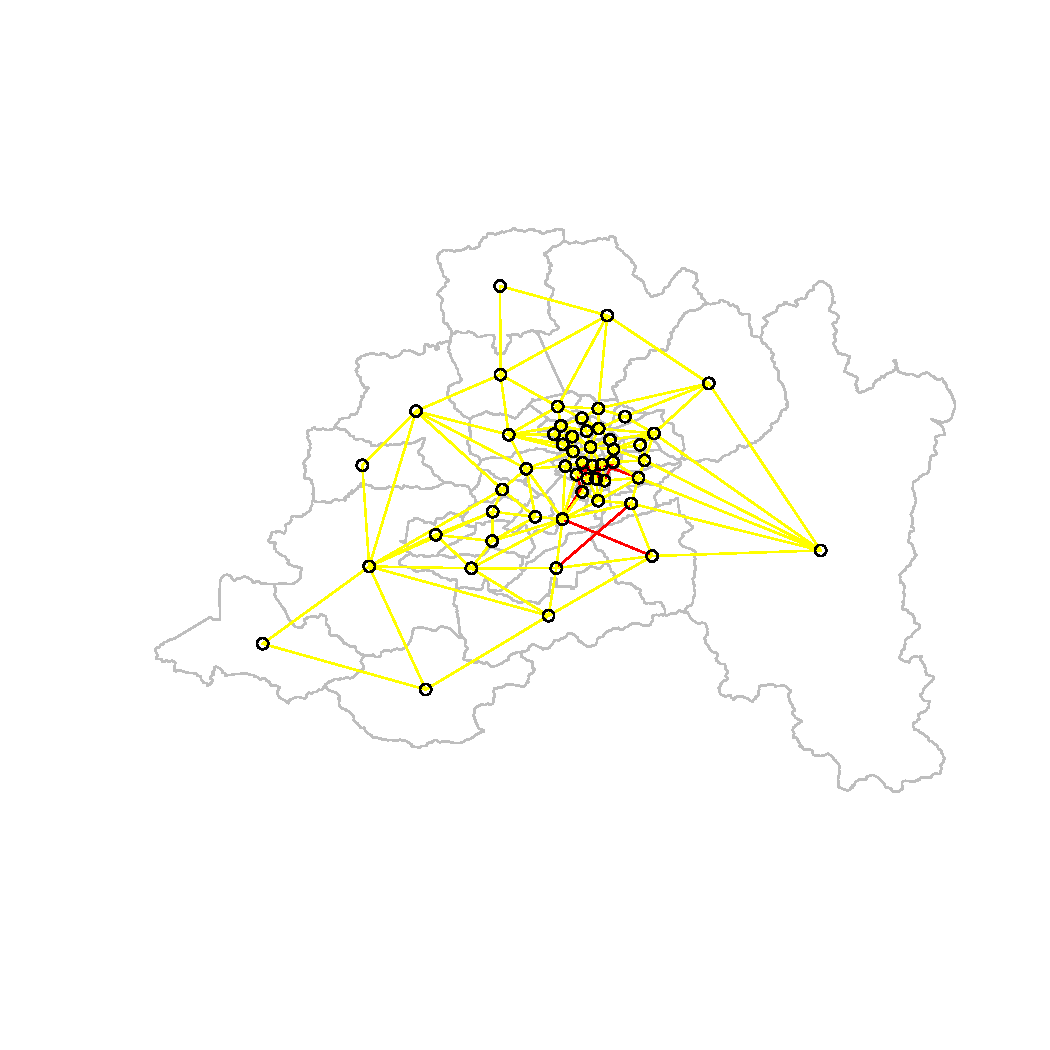
\includegraphics[width=8cm,height=8cm]{figure/plot-queen-rookT-1} 

}


\end{knitrout}
\end{figure}

%==================================================
\subsection{Creating Distance-based Neighbors}
%==================================================

We now construct spatial weight matrices using the $k$-nearest neighbors criteria\index{Weight matrix!knearneigh function}. 

\begin{knitrout}
\definecolor{shadecolor}{rgb}{0.969, 0.969, 0.969}\color{fgcolor}\begin{kframe}
\begin{alltt}
\hlcom{# K-neighbors}
\hlstd{coords} \hlkwb{<-} \hlkwd{coordinates}\hlstd{(mr)}                             \hlcom{# coordinates of centroids}
\hlkwd{head}\hlstd{(coords,} \hlnum{5}\hlstd{)}                                       \hlcom{# show coordinates}
\end{alltt}
\begin{verbatim}
##        [,1]      [,2]
## 0 -70.65599 -33.45406
## 1 -70.71742 -33.50027
## 2 -70.74504 -33.42278
## 3 -70.67735 -33.38372
## 4 -70.67640 -33.56294
\end{verbatim}
\begin{alltt}
\hlstd{k1neigh} \hlkwb{<-} \hlkwd{knearneigh}\hlstd{(coords,} \hlkwc{k} \hlstd{=} \hlnum{1}\hlstd{,} \hlkwc{longlat} \hlstd{=} \hlnum{TRUE}\hlstd{)}  \hlcom{# 1-nearest neighbor}
\hlstd{k2neigh} \hlkwb{<-} \hlkwd{knearneigh}\hlstd{(coords,} \hlkwc{k} \hlstd{=} \hlnum{2}\hlstd{,} \hlkwc{longlat} \hlstd{=} \hlnum{TRUE}\hlstd{)}  \hlcom{# 2-nearest neighbor}
\end{alltt}
\end{kframe}
\end{knitrout}

The function \code{coords} extract the spatial coordinates from the shape file, whereas the function \code{knearneigh} returns a matrix with the indices of points belonging to the set of the $k$-nearest neighbors of each other. The argument \code{k} indicates the number of nearest neighbors to be returned. If point coordinates are longitude-latitude decimal degrees, then distances are measured in kilometers if \code{longlat = TRUE}. Furthermore, if \code{longlat = TRUE}, great circle distances are used. Note that the objects \code{k1neigh} and \code{k2neigh} are of class \code{knn}.

Weight matrices based on inverse distance can be computed in the following way (see Section \ref{sec:inverse_distance}):

\begin{knitrout}
\definecolor{shadecolor}{rgb}{0.969, 0.969, 0.969}\color{fgcolor}\begin{kframe}
\begin{alltt}
\hlcom{# Inverse weight matrix}
\hlstd{dist.mat} \hlkwb{<-} \hlkwd{as.matrix}\hlstd{(}\hlkwd{dist}\hlstd{(coords,} \hlkwc{method} \hlstd{=} \hlstr{"euclidean"}\hlstd{))}
\hlstd{dist.mat[}\hlnum{1}\hlopt{:}\hlnum{5}\hlstd{,} \hlnum{1}\hlopt{:}\hlnum{5}\hlstd{]}
\end{alltt}
\begin{verbatim}
##            0          1          2          3          4
## 0 0.00000000 0.07687010 0.09438408 0.07350782 0.11078109
## 1 0.07687010 0.00000000 0.08226867 0.12324109 0.07489489
## 2 0.09438408 0.08226867 0.00000000 0.07814455 0.15606360
## 3 0.07350782 0.12324109 0.07814455 0.00000000 0.17922003
## 4 0.11078109 0.07489489 0.15606360 0.17922003 0.00000000
\end{verbatim}
\begin{alltt}
\hlstd{dist.mat.inv} \hlkwb{<-} \hlnum{1} \hlopt{/} \hlstd{dist.mat} \hlcom{# 1 / d_\{ij\}}
\hlkwd{diag}\hlstd{(dist.mat.inv)} \hlkwb{<-} \hlnum{0}      \hlcom{# 0 in the diagonal}
\hlstd{dist.mat.inv[}\hlnum{1}\hlopt{:}\hlnum{5}\hlstd{,} \hlnum{1}\hlopt{:}\hlnum{5}\hlstd{]}
\end{alltt}
\begin{verbatim}
##           0         1         2         3         4
## 0  0.000000 13.008960 10.595007 13.603994  9.026811
## 1 13.008960  0.000000 12.155295  8.114177 13.352046
## 2 10.595007 12.155295  0.000000 12.796797  6.407644
## 3 13.603994  8.114177 12.796797  0.000000  5.579733
## 4  9.026811 13.352046  6.407644  5.579733  0.000000
\end{verbatim}
\begin{alltt}
\hlcom{# Standardized inverse weight matrix}
\hlstd{dist.mat.inve} \hlkwb{<-} \hlkwd{mat2listw}\hlstd{(dist.mat.inv,} \hlkwc{style} \hlstd{=} \hlstr{"W"}\hlstd{,} \hlkwc{row.names} \hlstd{= mr}\hlopt{$}\hlstd{NAME)}
\hlkwd{summary}\hlstd{(dist.mat.inve)}
\end{alltt}
\begin{verbatim}
## Characteristics of weights list object:
## Neighbour list object:
## Number of regions: 52 
## Number of nonzero links: 2652 
## Percentage nonzero weights: 98.07692 
## Average number of links: 51 
## Link number distribution:
## 
## 51 
## 52 
## 52 least connected regions:
## Santiago Cerillos Cerro Navia Conchali El Bosque Estacion Central La Cisterna La Florida La Granja La Pintana La Reina Lo Espejo Lo Prado Macul Nunoa Pedro Aguirre Cerda Penalolen Providencia Quinta Normal Recoleta Renca San Joaquin San Miguel San Ramon Independencia Puente Alto Las Condes Vitacura Quilicura Huechuraba Maipu Pudahuel San Bernardo Tiltil Lampa Colina Lo Barnechea Pirque Paine Buin Alhue Melipilla San Pedro Maria Pinto Curacavi Penaflor Calera de Tango Padre Hurtado El Monte Talagante Isla de Maipo San Jose de Maipo with 51 links
## 52 most connected regions:
## Santiago Cerillos Cerro Navia Conchali El Bosque Estacion Central La Cisterna La Florida La Granja La Pintana La Reina Lo Espejo Lo Prado Macul Nunoa Pedro Aguirre Cerda Penalolen Providencia Quinta Normal Recoleta Renca San Joaquin San Miguel San Ramon Independencia Puente Alto Las Condes Vitacura Quilicura Huechuraba Maipu Pudahuel San Bernardo Tiltil Lampa Colina Lo Barnechea Pirque Paine Buin Alhue Melipilla San Pedro Maria Pinto Curacavi Penaflor Calera de Tango Padre Hurtado El Monte Talagante Isla de Maipo San Jose de Maipo with 51 links
## 
## Weights style: W 
## Weights constants summary:
##    n   nn S0       S1       S2
## W 52 2704 52 2.902384 214.3332
\end{verbatim}
\end{kframe}
\end{knitrout}

The function \code{dist} from \pkg{stats} package computes and returns the distance matrix computed by using the specified distance measure---euclidean distance in this example--- to compute the distance between the rows of a data matrix. The other methods that can be used are \code{maximum}, \code{manhattan}, \code{canberra}, \code{binary} or \code{minkowski}. Finally, the \code{mat2listw} function converts a square spatial weight matrix as a sequence of number \code{1:nrow(x)}.\footnote{For more about spatial weight matrices see \citep{stewart2010choosing}.}

%Another approach is the so-called sphere of influence neighbors

%<<other-dist, message =  FALSE>>=
%mr.tri.nb <- tri2nb(coords = coords)
%summary(mr.tri.nb)
%mr.gab.nb <- graph2nb(gabrielneigh(coords), sym = TRUE)
%mr.rel.nb <- graph2nb(relativeneigh(coords), sym = TRUE)
%@

%The function \code{tri2nb} uses the \pkg{deldir} package to convert a matrix of two-dimensional coordinates into neighbours list of class \code{nb} with a list of integer vectors containing neighbour regions number IDs. 

The following code plot the different weight matrices: 


\begin{knitrout}
\definecolor{shadecolor}{rgb}{0.969, 0.969, 0.969}\color{fgcolor}\begin{kframe}
\begin{alltt}
\hlcom{# Plot Weights}
\hlkwd{par}\hlstd{(}\hlkwc{mfrow} \hlstd{=} \hlkwd{c}\hlstd{(}\hlnum{3}\hlstd{,} \hlnum{2}\hlstd{))}
\hlkwd{plot}\hlstd{(mr,} \hlkwc{border} \hlstd{=} \hlstr{"grey"}\hlstd{,} \hlkwc{main} \hlstd{=} \hlstr{"Queen"}\hlstd{)}
\hlkwd{plot}\hlstd{(queen.w,} \hlkwd{coordinates}\hlstd{(mr),} \hlkwc{add} \hlstd{=}  \hlnum{TRUE}\hlstd{,} \hlkwc{col} \hlstd{=} \hlstr{"red"}\hlstd{)}
\hlkwd{plot}\hlstd{(mr,} \hlkwc{border} \hlstd{=} \hlstr{"grey"}\hlstd{,} \hlkwc{main} \hlstd{=} \hlstr{"1-Neigh"}\hlstd{)}
\hlkwd{plot}\hlstd{(}\hlkwd{knn2nb}\hlstd{(k1neigh), coords,} \hlkwc{add} \hlstd{=} \hlnum{TRUE}\hlstd{,} \hlkwc{col} \hlstd{=} \hlstr{"red"}\hlstd{)}
\hlkwd{plot}\hlstd{(mr,} \hlkwc{border} \hlstd{=} \hlstr{"grey"}\hlstd{,} \hlkwc{main} \hlstd{=} \hlstr{"2-Neigh"}\hlstd{)}
\hlkwd{plot}\hlstd{(}\hlkwd{knn2nb}\hlstd{(k2neigh),} \hlkwd{coordinates}\hlstd{(mr),} \hlkwc{add} \hlstd{=} \hlnum{TRUE}\hlstd{,} \hlkwc{col} \hlstd{=} \hlstr{"red"}\hlstd{)}
\hlkwd{plot}\hlstd{(mr,} \hlkwc{border} \hlstd{=} \hlstr{"grey"}\hlstd{,} \hlkwc{main} \hlstd{=} \hlstr{"Inverse Distance"}\hlstd{)}
\hlkwd{plot}\hlstd{(dist.mat.inve,} \hlkwd{coordinates}\hlstd{(mr),} \hlkwc{add} \hlstd{=}  \hlnum{TRUE}\hlstd{,} \hlkwc{col} \hlstd{=} \hlstr{"red"}\hlstd{)}
\end{alltt}
\end{kframe}
\end{knitrout}


\begin{figure}[h!]
  \caption{Different Spatial Weight Schemes for MR}
    \label{fig:more_ws}
\begin{knitrout}
\definecolor{shadecolor}{rgb}{0.969, 0.969, 0.969}\color{fgcolor}

{\centering 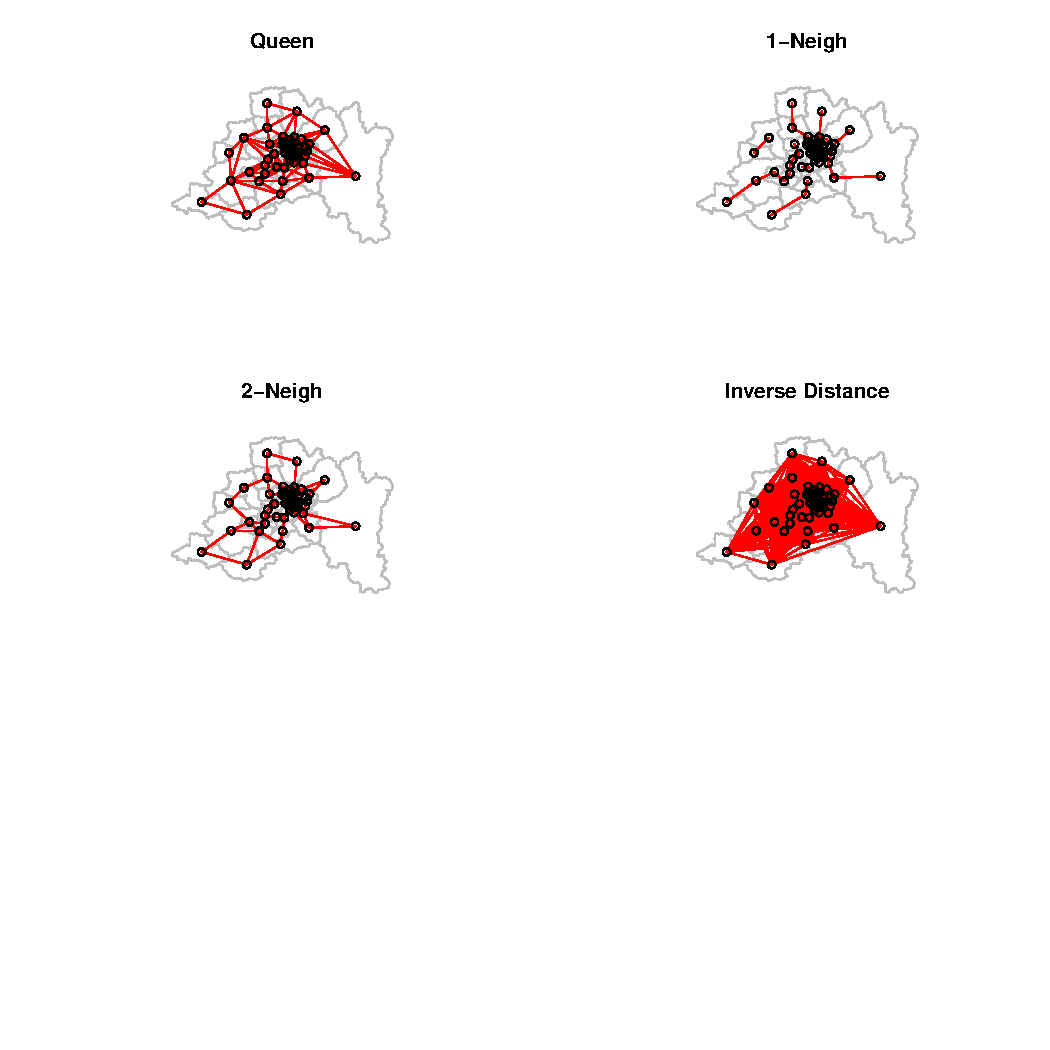
\includegraphics[width=\maxwidth]{figure/plot-all-wsT-1} 

}


\end{knitrout}
\end{figure}

\subsection{Constructing a Spatially Lagged Variable}

Spatially lagged variables are important elements of many spatial test and spatial regression specifications. In \pkg{spdep}, they are constructed by means of the \code{lag.listw} function.

First, we will combine the variables \code{POVERTY} and \code{URB\_POP} into a matrix and check the contents with \code{head}

\begin{knitrout}
\definecolor{shadecolor}{rgb}{0.969, 0.969, 0.969}\color{fgcolor}\begin{kframe}
\begin{alltt}
\hlcom{# X matrix}
\hlstd{X} \hlkwb{<-} \hlkwd{cbind}\hlstd{(mr}\hlopt{$}\hlstd{POVERTY, mr}\hlopt{$}\hlstd{URB_POP)}
\hlkwd{head}\hlstd{(X,} \hlnum{5}\hlstd{)}
\end{alltt}
\begin{verbatim}
##      [,1]   [,2]
## [1,]    8 159919
## [2,]    9  65262
## [3,]   18 131850
## [4,]   12 104634
## [5,]   14 166514
\end{verbatim}
\end{kframe}
\end{knitrout}

Now, we can construct a spatially lagged version of this matrix, using the \code{queen.w} weights\index{Weight matrix!lag.listw function}:

\begin{knitrout}
\definecolor{shadecolor}{rgb}{0.969, 0.969, 0.969}\color{fgcolor}\begin{kframe}
\begin{alltt}
\hlcom{# Create WX}
\hlstd{WX} \hlkwb{<-} \hlkwd{lag.listw}\hlstd{(}\hlkwd{nb2listw}\hlstd{(queen.w), X)}
\hlkwd{head}\hlstd{(WX)}
\end{alltt}
\begin{verbatim}
##          [,1]     [,2]
## [1,]  9.10000 100138.9
## [2,] 12.40000 299498.4
## [3,] 14.00000 144756.5
## [4,] 14.60000 121974.2
## [5,] 18.25000 170266.5
## [6,] 10.42857 236231.1
\end{verbatim}
\end{kframe}
\end{knitrout}


%****************************************************
\section{Testing for Spatial Autocorrelation}
%*****************************************************

As we stated in Section \ref{sec:Spatial_autocorrelation}, spatial autocorrelation refers to the correlation of a variable with itself in space. It can be positive (when high values correlate with high neighboring values or when low values correlate with low neighboring values) or negative (spatial outlier for high-low or low-high values). So the next question is how to test whether the spatial pattern we observe truly follows a spatial autocorrelated process or is completely random. In other words, we need a test of spatial autocorrelation to formally examine whether the observed value of a variable at one location is independent of values of that variable at neighboring locations.

%=============================================================
\subsection{Global Spatial Autocorrelation: Moran's I}\label{sec:moransI}
%============================================================

Global spatial autocorrelation is a measure of overall clustering. So the main goal of these indices is to summarize the degree to which similar observations tend to occur near each other. Those indices calculate the similarity of values at location $i$ and $j$ then `weight' the similarity by the proximity of locations $i$ and $j$. High similarities with high weight indicate similar values that are close together, whereas low similarities with high weight indicate dissimilar values that are close together.

The most general measure used is the Moran's I.\footnote{There exists several other measures of global spatial autocorrelation as the Geary's $C$ test. But, in this notes we will focus only in the Moran's I.} This statistic is a measure of overall clustering that exists in a dataset. It is assessed by means of a test of a null hypothesis of random location. Therefore, rejection of this null hypothesis suggests a spatial pattern or spatial structure. 

Moran's I is given by\index{Moran's I test}:

\begin{equation}\label{eq:I-moran}
I = \frac{\sum_{i = 1}^n\sum_{j=1, j\neq i}^n w_{ij}\left(x_i - \bar{x}\right)\left(x_j - \bar{x}\right)}{S_0 \sum_{i = 1}^n\left(x_i - \bar{x}\right)^2/n} = \frac{n\sum_{i = 1}^n\sum_{j=1}^n w_{ij}\left(x_i - \bar{x}\right)\left(x_j - \bar{x}\right)}{S_0 \sum_{i = 1}^n\left(x_i - \bar{x}\right)^2}
\end{equation}
%
where $S_0=\sum_{i = 1}^n\sum_{j=1}^nw_{ij}$ and $w_{ij}$ is an element of the spatial weight matrix that measures spatial distance or connectivity between regions $i$ and $j$. In matrix form:


\begin{equation*}
	I = \frac{n}{S_0} \frac{\vz^\top\mW\vz}{\vz^\top\vz}
\end{equation*}
%
where: 


\begin{equation*}
\vz = \begin{pmatrix}
          x_1 - \bar{x}\\
          x_2 - \bar{x} \\
          \vdots\\
          x_n - \bar{x}
      \end{pmatrix}
\end{equation*}

If the $\mW$ matrix is row standardized, then:

\begin{equation*}
	I = \frac{\vz^\top\mW^s\vz}{\vz^\top\vz}
\end{equation*}
%
because $S_0=n$. Values range from -1 (perfect dispersion) to +1 (perfect correlation). A zero value indicates a random spatial pattern. 


A very useful tool for understanding the Moran’s I test is the Moran Scatterplot. The idea of the Moran scatterplot is to display the variable for each region (on the horizontal axis) against the standardized spatial weighted average (average of the neighbors' $x$, also called spatial lag) on the vertical axis (See Figure \ref{fig:moran_scatterplot}). As pointed out by \cite{anselin1996chapter}, expressing the variables in standardized from (i.e. with mean zero and standard deviation equal to one) allows assessment of both the global spatial association, since the slope of the line is the Moran's I coefficient, and local spatial association (the quadrant in the scatterplot). The Moran scatterplot is therefore divided into four different quadrants corresponding to the four types of local spatial association between a region and its neighbors\index{Moran's I test!Moran scatterplot}:

\begin{itemize}
  \item Quadrant I displays the region with high $x$ (above the average) surrounded by regions with high $x$ (above the average). This quadrant is usually  denoted High-High.
  \item Quadrant II show the regions with low value surrounded by region with high values. This quadrant is usually denoted Low-High.
  \item Quadrant III display the regions with low value surrounded by regions with low values, and is denoted Low-Low.
  \item Quadrant IV shows the regions with high value surrounded by regions with low values. It is noted High-Low.
\end{itemize}

Regions located in quadrant I and III refer to positive spatial autocorrelation, the spatial clustering of similar values, whereas quadrant II and IV represent negative spatial autocorrelation, the spatial clustering of dissimilar values. 

\begin{figure}[ht]
  \caption{Moran Scatterplot}\label{fig:moran_scatterplot}
\begin{knitrout}
\definecolor{shadecolor}{rgb}{0.969, 0.969, 0.969}\color{fgcolor}

{\centering 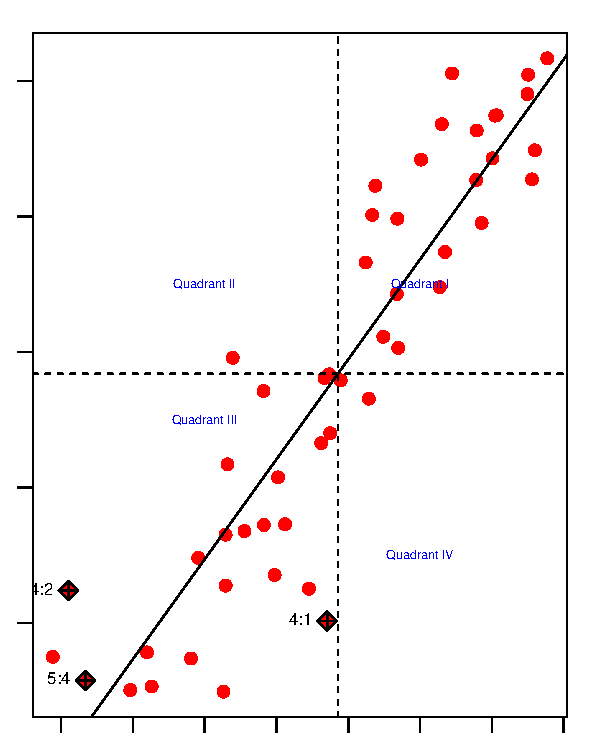
\includegraphics[width=\maxwidth]{figure/moran-1} 

}


\end{knitrout}
\end{figure}


To understand Moran's I, it is important to note the similarity of the Moran's $I$ with the OLS coefficient. Recall that 

\begin{equation}
  \widehat{\vbeta}= \frac{\sum_{i = 1}^n\left(x_i - \bar{x}\right)(y_i - \bar{y})}{\sum_{i = 1}^n \left(x_i - \bar{x}\right)^2}
\end{equation}

Then looking at (\ref{eq:I-moran}), Moran's $I$ is equivalent to the slope coefficient of a linear regression of the spatial lag $\mW\vx$ on the observation vector $\vx$ measured in deviation from their mean. It is, however, not equivalent to the slope of $\vx$ on $\mW\vx$ which would be a more natural way. 

The hypothesis tested by the Moran's $I$ is the following:

\begin{itemize}
  \item $H_0$: $\vx$ is spatially independent; the observed $\vx$ is assigned at random among locations. In this case $I$ is close to zero.
  \item $H_1$: $\vx$ is not spatially independent. In this case $I$ is statistically different from zero. 
\end{itemize}

What is the distribution of the Moran's I? We are interested in the distribution of:

\begin{equation*}
  \frac{I - \E\left[I\right]}{\sqrt{\var(I)}}
\end{equation*}

There are two ways to compute the mean and variance of Moran's I. The first one is under the normal assumption of $x_i$ and the second one is under randomization of $x_i$. Under the normal assumption, it is assumed that the random variable $x_i$ are the result of $n$ independently drawings from a normal population. Under the randomization assumption, no matter what the underlying distribution of the populations, we consider the observed values of $x_i$ were repeatedly randomly permuted.

\subsubsection{Moments Under Normality Assumption}

Theorem \ref{teo:Moran_normal} gives the moments of Moran's I under normality. 

\begin{theorem}[Moran's $I$ Under Normality]\label{teo:Moran_normal}\index{Moran's I test!Normality}
Assume that $\left\lbrace \vx_i\right\rbrace = \left\lbrace x_1, x_2,..., x_n\right\rbrace$ are independent and distributed as $\rN(\mu, \sigma^2)$, but $\mu$ and $\sigma^2$ are unknown. Then:

\begin{equation}
\E\left(I\right) = - \frac{1}{n - 1} 
\end{equation}
%
and

\begin{equation}
\E\left(I^2\right) = \frac{n^2S_1 - nS_2 + 3S_0^2}{S_0^2(n^2 - 1)}
\end{equation}
%
where $S_0=\sum_{i = 1}^n\sum_{j=1}^nw_{ij}$, $S_1= \sum_{i = 1}^n\sum_{j = 1}^n(w_{ij} + w_{ji})^2/2$, $S_2 = \sum_{i = 1}^n(w_{i.} + w_{.i})^2$, where $w_{i.}= \sum_{j = 1}^nw_{ij}$ and $w_{i.}=\sum_{j = 1}^nw_{ji}$
Then:

\begin{equation}
\var\left(I\right)=\E\left(I^2\right) - \E\left(I\right)^2
\end{equation}
\end{theorem}

\begin{proof}
Let $z_i=x_i - \bar{x}$. The following moments are true for $z_i$:

\begin{eqnarray*}
\E\left[z_i\right]   & = & 0 \\
\E\left[z_i^2\right] & = & \sigma^2 - \frac{\sigma^2}{n} \\
\E\left[z_iz_j\right] & = & - \frac{\sigma^2}{n} \\
\E\left[z_i^2 z_j^2\right] & = & \frac{(n^2 - 2n + 3)\sigma^2}{m^2} \\
\E\left[z_i^2 z_jz_k\right] & = & - \frac{(n -3)\sigma^4}{n} \\
\E\left[z_iz_jz_kz_l\right] & = & \frac{3 \sigma^4}{n^2}
\end{eqnarray*}


Then:

\begin{equation}
  \begin{aligned}
    \E\left[I\right] & = \frac{n}{S_0}\frac{\E\left[\sum_{i = 1}^n\sum_{j=1}^nw_{ij}z_iz_j\right]}{\E\left[\sum_{i=1}^nz_i^2\right]}
    & = \frac{n}{S_0}\sum_{i = 1}^n\sum_{j=1}^nw_{ij}\frac{\E\left[z_iz_j\right]}{\sum_{i=1}^n\E\left[z_i^2\right]} \\
    & = \frac{-nS_0\frac{\sigma^2}{n}}{S_0 n (1 - 1/n)\sigma^2 } \\
    & = -\frac{\frac{\sigma^2}{n}}{(1 - 1/n)\sigma^2 } \\
    & = -\frac{1}{n - 1} 
  \end{aligned}
\end{equation}

and

\begin{equation}
  \begin{aligned}
    \E\left[I^2\right] & = \E\left[\frac{n^2}{S_0^2}\frac{\left[\sum_{i = 1}^n\sum_{j=1}^nw_{ij}z_iz_j\right]^2}{\left[\sum_{i=1}^nz_i^2\right]^2}\right] \\
    & = \frac{n^2}{S_0^2} \E\left[\frac{1/2\sum_{(2)}(w_{ij} + w_{ji})^2 z_i^2 z_j^2 + \sum_{(3)}(w_{ij} + w_{ji})(w_{ik} + w_{ki})z_i^2z_jz_k + \sum_{(4)} w_{ij}w_{kl}z_iz_jz_kz_l}{s}\right]
  \end{aligned}
\end{equation}
\end{proof}

\subsubsection{Moran's $I$ under Randomization}

%Recall that when testing a null hypothesis we need a test statistic that will have different values under the null hypothesis and the alternatives. We then need to compute the sampling distribution of the test statistic when the null hypothesis is true. For some test statistics and some null hypotheses this can be done analytically. Then, the $p$-value is the probability that the test statistic would be at least as extreme as we observed, if the null hypothesis is true.

%A permutation test gives a simple way to compute the sampling distribution for any test statistic. 

%To estimate the sampling distribution of the test statistic we need many samples generated under the strong null hypothesis. A permutation test builds sampling distribution by resampling the observed data. Specifically, we can ``shuffle'' or permute the observed data by 


%A randomization test (also called a permutation test) is a type of statistical significance test in which the distribution of the test statistic under the null hypothesis is obtained by calculating all possible values of the test statistics under rearrangements of the labels on the observed points. 

%No matter what the underlying distribution of the population, we consider the observed values of $x_i$ were repeatedly randomly permuted.


%Under randomization 

%The testing method under randomization assumption is called permutation test. 

Theorem \ref{teo:Moran_random} gives the moments of Moran's I under randomization. 


\begin{theorem}[Moran's $I$ Under Randomization]\label{teo:Moran_random}\index{Moran's I test!Randomization}
Under permutation, we have:

\begin{equation}
\E\left(I\right) = - \frac{1}{n - 1} 
\end{equation}
%
and

\begin{equation}
\E\left(I^2\right) = \frac{n\left[\left(n^2 - 3n + 3\right)S_1 - nS_2 + 3S_0^2\right]-b_2\left[\left(n^2 - n\right)S_1 - 2nS_2 + 6S_0^2\right]}{(n-1)(n-2)(n-3)S_0^2}
\end{equation}
%
where $S_0=\sum_{i = 1}^n\sum_{j=1}^nw_{ij}$, $S_1= \sum_{i = 1}^n\sum_{j = 1}^n(w_{ij} + w_{ji})^2/2$, $S_2 = \sum_{i = 1}^n(w_{i.} + w_{.i})^2$, where $w_{i.}= \sum_{j = 1}^nw_{ij}$ and $w_{i.}=\sum_{j = 1}^nw_{ji}$.Then:

\begin{equation}
\var\left(I\right)=\E\left(I^2\right) - \E\left(I\right)^2
\end{equation}
\end{theorem}

It is important to note that the expected value of Moran's $I$ under normality and randomization is the same. 

\subsubsection{Monte Carlo Moran's $I$}

The normality assumption is a very strong assumption. However we can use the Moran’s I test based on Monte Carlo simulation.

The idea for any Monte Carlo test is the following\index{Moran's I test!Monte carlo}: 

\begin{itemize}
  \item To test a null hypothesis $H_0$ (no spatial autocorrelation in our case), we specify a test statistic $T$ such that large values of $T$ are evidence against $H_0$.
  \item Let $T$ have observed value $t_{obs}$. We generally want to compute
  
  \begin{equation}
    p-value = \Pr(T\geq t_{obs}|H_0)
  \end{equation}
  
  Therefore we need the distribution of $T$ when $H_0$ is true to evaluate this probability.
\end{itemize}

The algorithm for the Morans' I Monte Carlo test is the following:

\begin{algorithm}[Moran's' I Monte Carlo Test]
The procedure is the following:

\begin{enumerate}
\item Rearrange the spatial data by shuffling their location and compute the Moran's I $S$ times. This will create the distribution under $H_0$. This operationalizes spatial randomness. 
\item Let $I_1^*, I_2^*,..., I_S^*$ be the Moran's I for each time. A consistent Monte Carlo p-value is then:
  \begin{equation}
    \widehat{p} = \frac{1 + \sum_{s=1}^S 1(I^*_s \geq I_{obs})}{S + 1}
  \end{equation}
  \item For tests at the $\alpha$ level or at $100(1- \alpha)\%$ confidence intervals, there are reasons for choosing $S$ so that $\alpha(S + 1)$ is an integer. For example, use $S=999$ for confidence intervals and hypothesis tests when $\alpha = 0.05$.
\end{enumerate}
\end{algorithm}


%%=====================================================
%\subsection{Local Indicators of Spatial Association (LISA)}
%=====================================================

%\cite{anselin1995local} suggests that a local indicator of spatial association (LISA) is any statistic that satisfies the following two requirements:

%\begin{enumerate}
%  \item the LISA for each observation gives an indication of the extent of significant spatial clustering of similar values around that observation;
%  \item the sum of LISAs for all observations is proportional to a global indicator of spatial association.
%\end{enumerate}

%=====================================================
\section{Application: Poverty in Santiago, Chile}
%=====================================================

In this section we undertake and exploratory spatial data analysis (ESDA) for poverty in Metropolitan Region, Chile.  We start by loading the required packages and the shape file. 

\begin{knitrout}
\definecolor{shadecolor}{rgb}{0.969, 0.969, 0.969}\color{fgcolor}\begin{kframe}
\begin{alltt}
\hlcom{# Load maptools ----}
\hlkwd{library}\hlstd{(}\hlstr{"maptools"}\hlstd{)} \hlcom{# Tools for reading and handling spatial objects}
\hlkwd{library}\hlstd{(}\hlstr{"RColorBrewer"}\hlstd{)}
\hlkwd{library}\hlstd{(}\hlstr{"spdep"}\hlstd{)}
\hlstd{mr} \hlkwb{<-} \hlkwd{readShapeSpatial}\hlstd{(}\hlstr{"mr_chile"}\hlstd{)}
\end{alltt}
\end{kframe}
\end{knitrout}

%================================
\subsection{Cloropeth Graphs}
%================================


If we are interested in the geographical variation in poverty, we should start by plotting the spatial distribution of poverty.  This can be useful in a variety of way.  Usually, aggregate or national level indicators hide important differences between different spatial units. Thus, poverty mapping helps to highlight geographical variations.  In addition to this, another advantage of poverty maps is their legibility- maps are powerful tools for representing complex information in a visual format that is easy to understand. 


So, we start by plotting the geographical variation of poverty among communes by using the \code{spplot} function. In particular, we use a cloropleth\footnote{The name of this technique is derived from the Greek words choros - space, and pleth - value} map using the quantile classification. In a quantile graph, the variable is sorted and grouped in categories with equal number of observations, or quantiles. 


\begin{knitrout}
\definecolor{shadecolor}{rgb}{0.969, 0.969, 0.969}\color{fgcolor}\begin{kframe}
\begin{alltt}
\hlcom{# Cloropleth graphs ----}
\hlkwd{spplot}\hlstd{(}\hlkwc{obj} \hlstd{= mr,}
       \hlkwc{zcol} \hlstd{=} \hlstr{"POVERTY"}\hlstd{,}
       \hlkwc{at} \hlstd{=} \hlkwd{quantile}\hlstd{(mr}\hlopt{$}\hlstd{POVERTY,} \hlkwc{p} \hlstd{=} \hlkwd{c}\hlstd{(}\hlnum{0}\hlstd{,} \hlnum{.25}\hlstd{,} \hlnum{.5}\hlstd{,} \hlnum{.75}\hlstd{,} \hlnum{1}\hlstd{),}
                     \hlkwc{na.rm} \hlstd{=} \hlnum{TRUE}\hlstd{),}
       \hlkwc{col.regions} \hlstd{=} \hlkwd{brewer.pal}\hlstd{(}\hlnum{5}\hlstd{,} \hlstr{"Blues"}\hlstd{),}
       \hlkwc{main} \hlstd{=} \hlstr{"Cloropleth map of Metropolitan Region"}\hlstd{,}
       \hlkwc{sub} \hlstd{=} \hlstr{"Poverty"}\hlstd{)}
\end{alltt}
\end{kframe}
\end{knitrout}

Figure \ref{fig:cloro-graph} provides some useful insights. First, it clearly shows that the spatial pattern of poverty in the MR is not spatial homogeneous, but rather the intensity of poverty varies across space. Second, it provides an example of how disaggregated poverty indicators can reveal additional information to aggregate indicators. It shows that poverty intensity is lower peripheral communes than central communes. 

\begin{figure}
\caption{Cloropleth map: Poverty in the Metropolitan Region}\label{fig:cloro-graph}
\begin{knitrout}
\definecolor{shadecolor}{rgb}{0.969, 0.969, 0.969}\color{fgcolor}

{\centering 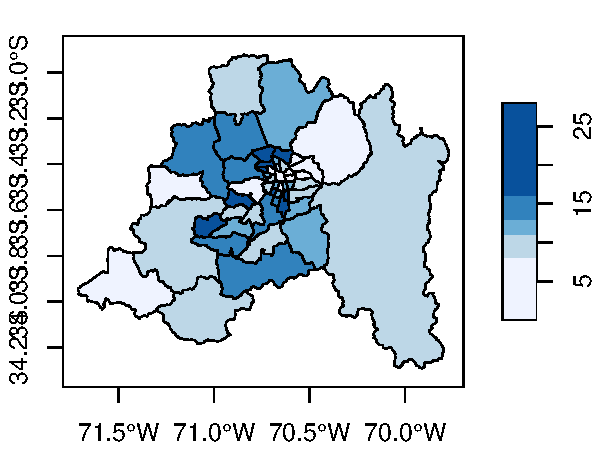
\includegraphics[width=\maxwidth]{figure/cloro-graphs-1} 

}


\end{knitrout}
\end{figure}

How to interpret quantile maps? A quantile classification scheme is an ordinal ranking of the data values, dividing the distribution into intervals that have an equal number of data values. Quantile classification ensures maps are easily comparable and can be `easy to read'.

We can also plot the data using the equal interval classification. Equal interval divides the data into equal size classes (e.g., 0-10, 10-20, 20-30, etc) and works best on data that is generally spread across the entire range. In the following example we use a defined interval classification. 

\begin{knitrout}
\definecolor{shadecolor}{rgb}{0.969, 0.969, 0.969}\color{fgcolor}\begin{kframe}
\begin{alltt}
\hlcom{# Define interval classification }
\hlstd{mr}\hlopt{$}\hlstd{pov.cat} \hlkwb{<-} \hlkwd{cut}\hlstd{(mr}\hlopt{$}\hlstd{POVERTY,}
                  \hlkwc{breaks} \hlstd{=} \hlkwd{c}\hlstd{(}\hlnum{0}\hlstd{,} \hlnum{9}\hlstd{,} \hlnum{12}\hlstd{,} \hlnum{16}\hlstd{,} \hlnum{28}\hlstd{),}
                  \hlkwc{labels} \hlstd{=} \hlkwd{c}\hlstd{(}\hlstr{"< 9"}\hlstd{,} \hlstr{"9-12"}\hlstd{,} \hlstr{"12-16"}\hlstd{,} \hlstr{">16"}\hlstd{))}
\hlkwd{spplot}\hlstd{(mr,} \hlstr{"pov.cat"}\hlstd{,} \hlkwc{col.regions} \hlstd{=} \hlkwd{brewer.pal}\hlstd{(}\hlnum{5}\hlstd{,} \hlstr{"Reds"}\hlstd{))}
\end{alltt}
\end{kframe}
\end{knitrout}

\begin{figure}[h]
\caption{Cloropleth map: Poverty in the Metropolitan Region (Equal Interval)}\label{fig:cloro-graph2}
\begin{knitrout}
\definecolor{shadecolor}{rgb}{0.969, 0.969, 0.969}\color{fgcolor}

{\centering 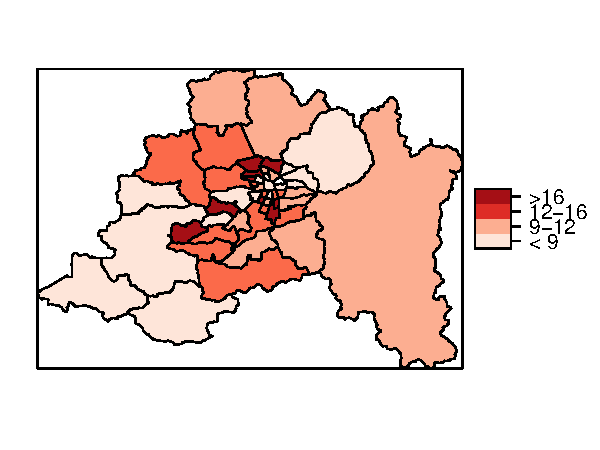
\includegraphics[width=\maxwidth]{figure/cloro-graphs2T-1} 

}


\end{knitrout}
\end{figure}


However, regarding the possible spatial association that seems to be derived from the above figures for the poverty variable, it is necessary to note that the results are sensitive to the number of defined intervals (among other things). Therefore, it is necessary to conduct a comprehensive and formal analysis about the potential presence of spatial dependence to ascertain whether there exists a pattern of statistically significant spatial autocorrelation in the spatial distribution of poverty. That is why now we calculate the Moran’s I test.


%================================
\subsection{Moran's I Test}
%================================

First, we create two spatial weight matrices (queen and rook) to assess the robustness of the test under different spatial schemes. 

\begin{knitrout}
\definecolor{shadecolor}{rgb}{0.969, 0.969, 0.969}\color{fgcolor}\begin{kframe}
\begin{alltt}
\hlcom{# Generate W matrices}
\hlstd{queen.w} \hlkwb{<-} \hlkwd{poly2nb}\hlstd{(mr,} \hlkwc{row.names} \hlstd{= mr}\hlopt{$}\hlstd{NAME,} \hlkwc{queen} \hlstd{=}  \hlnum{TRUE}\hlstd{)}
\hlstd{rook.w}  \hlkwb{<-} \hlkwd{poly2nb}\hlstd{(mr,} \hlkwc{row.names} \hlstd{= mr}\hlopt{$}\hlstd{NAME,} \hlkwc{queen} \hlstd{=}  \hlnum{FALSE}\hlstd{)}
\end{alltt}
\end{kframe}
\end{knitrout}

Moran's I test statistic for spatial autocorrelation is implemented in \pkg{spdep} \citep{spdep}. There are mainly two function for computing this test: \code{moran.test}, where the inference is based on a normal or randomization assumption, and \code{moran.mc}, for a permutation-based test\index{Moran's I test!moran.test function}. 

\begin{knitrout}
\definecolor{shadecolor}{rgb}{0.969, 0.969, 0.969}\color{fgcolor}\begin{kframe}
\begin{alltt}
\hlcom{# Moran's I test}
\hlkwd{moran.test}\hlstd{(mr}\hlopt{$}\hlstd{POVERTY,} \hlkwc{listw} \hlstd{=} \hlkwd{nb2listw}\hlstd{(queen.w),} \hlkwc{randomisation} \hlstd{=} \hlnum{FALSE}\hlstd{,}
           \hlkwc{alternative} \hlstd{=} \hlstr{'two.sided'}\hlstd{)}
\end{alltt}
\begin{verbatim}
## 
## 	Moran I test under normality
## 
## data:  mr$POVERTY  
## weights: nb2listw(queen.w)    
## 
## Moran I statistic standard deviate = 4.0453, p-value = 5.225e-05
## alternative hypothesis: two.sided
## sample estimates:
## Moran I statistic       Expectation          Variance 
##       0.306497992      -0.019607843       0.006498517
\end{verbatim}
\begin{alltt}
\hlkwd{moran.test}\hlstd{(mr}\hlopt{$}\hlstd{POVERTY,} \hlkwc{listw} \hlstd{=} \hlkwd{nb2listw}\hlstd{(rook.w),} \hlkwc{randomisation} \hlstd{=} \hlnum{FALSE}\hlstd{,}
           \hlkwc{alternative} \hlstd{=} \hlstr{'two.sided'}\hlstd{)}
\end{alltt}
\begin{verbatim}
## 
## 	Moran I test under normality
## 
## data:  mr$POVERTY  
## weights: nb2listw(rook.w)    
## 
## Moran I statistic standard deviate = 4.3309, p-value = 1.485e-05
## alternative hypothesis: two.sided
## sample estimates:
## Moran I statistic       Expectation          Variance 
##       0.342282943      -0.019607843       0.006982432
\end{verbatim}
\end{kframe}
\end{knitrout}

The \code{randomisation} option is set to \code{TRUE} by default, which implies that in order to get inference based on a normal approximation, it must be explicitly set to \code{FALSE}, as in our case. Similarly, the default is a one-sided test, so that in order to obtain the results for the more commonly used two-sided test, the option \code{alternative} must be explicitly to \code{'two.sided'}. Note also that the \code{zero.policy} option is set to \code{FALSE} by default, which means that islands result in a missing value code \code{NA}. Setting this option to \code{TRUE} will set the spatial lag for island to the customary zero value. 

The results show that the Moran's I statistic are $\approx$ 0.30 and 0.34, respectively, and highly significant. This implies that there is evidence of robust \textbf{positive spatial autocorrelation} in the poverty variable (since we are rejecting the null hypothesis of random spatial distribution).


\begin{remark}
If you compute the Moran's I test for two different variables, but using the same spatial weight matrix, the expectation and variance of the Moran's I test statistic will be the same under the normal approximation. Why? 
\end{remark}

The test under randomization gives the following results:

\begin{knitrout}
\definecolor{shadecolor}{rgb}{0.969, 0.969, 0.969}\color{fgcolor}\begin{kframe}
\begin{alltt}
\hlcom{# Moran test under randomization}
\hlkwd{moran.test}\hlstd{(mr}\hlopt{$}\hlstd{POVERTY,} \hlkwc{listw} \hlstd{=} \hlkwd{nb2listw}\hlstd{(queen.w),}
           \hlkwc{alternative} \hlstd{=} \hlstr{'two.sided'}\hlstd{)}
\end{alltt}
\begin{verbatim}
## 
## 	Moran I test under randomisation
## 
## data:  mr$POVERTY  
## weights: nb2listw(queen.w)    
## 
## Moran I statistic standard deviate = 4.0689, p-value = 4.723e-05
## alternative hypothesis: two.sided
## sample estimates:
## Moran I statistic       Expectation          Variance 
##       0.306497992      -0.019607843       0.006423226
\end{verbatim}
\end{kframe}
\end{knitrout}

Note how the value of the statistic and its expectation do not change relative to the normal case, only the variance is different.

We can carry out a Moran's $I$ test based on random permutation the function \code{moran.mc}. Unlike previous test, it needs the number of permutations \code{nsim}. Since the rank of the observed statistic is computed relative to the reference distribution of statistics for the permuted data sets, it is good practice to set this number to something ending on 9 (such as 99 or 999). This will lead to rounded pseudo p-values like 0.01 or 0.001.\index{Moran's I test!moran.mc function} 


\begin{knitrout}
\definecolor{shadecolor}{rgb}{0.969, 0.969, 0.969}\color{fgcolor}\begin{kframe}
\begin{alltt}
\hlcom{# Moran's Test}
\hlkwd{set.seed}\hlstd{(}\hlnum{1234}\hlstd{)}
\hlkwd{moran.mc}\hlstd{(mr}\hlopt{$}\hlstd{POVERTY,} \hlkwc{listw} \hlstd{=} \hlkwd{nb2listw}\hlstd{(queen.w),}
           \hlkwc{nsim} \hlstd{=} \hlnum{99}\hlstd{)}
\end{alltt}
\begin{verbatim}
## 
## 	Monte-Carlo simulation of Moran I
## 
## data:  mr$POVERTY 
## weights: nb2listw(queen.w)  
## number of simulations + 1: 100 
## 
## statistic = 0.3065, observed rank = 100, p-value = 0.01
## alternative hypothesis: greater
\end{verbatim}
\end{kframe}
\end{knitrout}


Note that none of the permuted data sets yielded a Moran's $I$ greater than the observed value of 0.3065, hence a pseudo p-value of $(0 + 1) / (99 + 1) = 0.01$.

The Moran scatter plot can also be obtained using the function \code{moran.plot} of \pkg{spdep}:\index{Moran's I test!moran.plot function}

\begin{knitrout}
\definecolor{shadecolor}{rgb}{0.969, 0.969, 0.969}\color{fgcolor}\begin{kframe}
\begin{alltt}
\hlcom{# Moran's plot}
\hlkwd{moran.plot}\hlstd{(mr}\hlopt{$}\hlstd{POVERTY,} \hlkwc{listw} \hlstd{=} \hlkwd{nb2listw}\hlstd{(queen.w))}
\end{alltt}
\end{kframe}
\end{knitrout}

\begin{figure}[ht]
\caption{Moran Plot for Poverty}\label{fig:mp-poverty}
\begin{knitrout}
\definecolor{shadecolor}{rgb}{0.969, 0.969, 0.969}\color{fgcolor}

{\centering 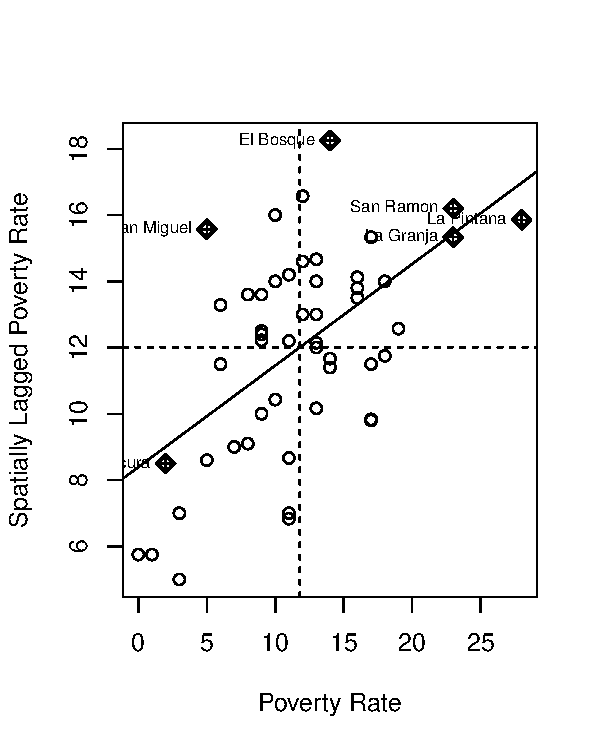
\includegraphics[width=\maxwidth]{figure/moran-plotT-1} 

}


\end{knitrout}
\end{figure}

Figure \ref{fig:mp-poverty} displays the Moran scatterplot of poverty with the queen weight matrix. Positive spatial autocorrelation, detected by the value of the Moran's I, is reflected by the fact that most of the communes are located in quadrant I and III. However, there are some exceptions such as the communes located in quadrant II and IV. For example, San Miguel is a commune with low poverty rate, but surrounded by communes with high poverty.  

A major limitation of Moran's I is that it cannot provide information on the specific locations of spatial patterns; it only indicates the presence of spatial autocorrelation globally. A single overall indication is given of whether spatial autocorrelation exists in the dataset, but no indication is given of whether local variations exist in spatial autocorrelation (e.g., concentrations, outliers) across the spatial extent of the data. 


%==============================
\chapter{Spatial Models}
%==============================

Previously, we have reviewed some preliminary concepts in spatial econometric, such as spatial dependency and spatial autocorrelation. In this chapter we will analyze the formulation of spatial models. In particular, in Section \ref{sec:taxonomy} we will derive a complete taxonomy of spatial models including the Spatial Lag Model, Spatial Durbin Model, Spatial Error Model and the Spatial Autocorrelation Model. We will give a brief motivation of each of them and some examples.  In Section \ref{sec:interpretation} we show how to understand the `spillover' effects and how to interpret marginal effects in the spatial model framework. 

%*******************************
\section{Taxonomy of Models}\label{sec:taxonomy}
%*******************************

As we showed in previous chapter (in particular in Section~\ref{sec:spatial_dependence}), it is no possible to model spatial dependencies using traditional econometrics. The main problem is that we have more parameters than observations. However, using the spatial weight matrix we can solve that problem by reducing the number of parameters to just one parameter using the weighted average of the $\vy$ values in the neighborhood of $i$. 

\subsection{Spatial Lag Model}\index{Spatial lag model}

So, given the problem of insufficient degree of freedom, how to model a situation where the dependent variable depends also of the spatially lagged variable? Instead of using a full system of equation, we can model the spatial dependency as:

\begin{equation}\label{eq:slm_model_1}
y_i = \alpha +\rho \sum_{j = 1}^n w_{ij}y_j + \epsilon_i, \quad i = 1,...,n,
\end{equation}
%
where $w_{ij}$ is the $(i,j)$th element of the spatial weight matrix $\mW$ matrix (see Definition \ref{def:W}); $y_i$ is the dependent variable for spatial unit $i$, so that $\sum_{j = 1}^n w_{ij}y_j$ is the weighted average of the dependent variable for the neighbors of $i$ (or spatial lag); $\epsilon_i$ is the error term such that $\E(\epsilon_i)= 0$; and $\rho$ is the spatial autoregressive parameter which measures the intensity of the spatial interdependence: $\rho > 0$ indicates a positive spatial dependence, whereas $\rho < 0$ indicates a negative spatial dependence. It should be clear that if $\rho = 0$, then we have the traditional linear regression model. By including a spatially lagged variable we are making explicit the the existence of spatial spillovers effects due to, for example, geographical proximity. This data generating process is known as a \emph{Spatial Autoregressive Process}\index{Spatial autoregressive process} or also labeled as SAR or \emph{Spatial Lag Model} SLM. Since the model (\ref{eq:slm_model_1}) does not include explanatory variables the model is known as the pure SLM or SAR model. 

\begin{figure}[ht]

	\caption{The SLM for two tegions}\label{figure:slm}
		\centering
		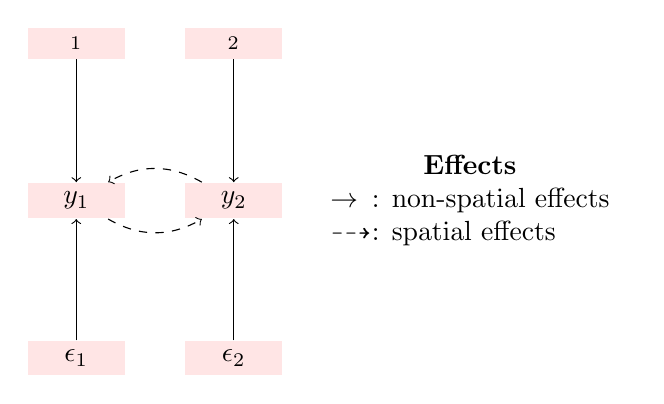
\begin{tikzpicture}
			\node[rectangle, text  width = 1cm, fill = red!10, align = center] (y1) at (-1,0) {$y_1$};
			\node[rectangle, text  width = 1cm, fill = red!10, align = center] (x1) at (-1,2) {$\vx_1$};
			\node[rectangle, text  width = 1cm, fill = red!10, align = center] (e1) at (-1,-2) {$\epsilon_1$};
			\node[rectangle, text  width = 1cm, fill = red!10, align = center] (y2) at (1, 0) {$y_2$};
			\node[rectangle, text  width = 1cm, fill = red!10, align = center] (x2) at (1,2) {$\vx_2$};
			\node[rectangle, text  width = 1cm, fill = red!10, align = center] (e2) at (1,-2) {$\epsilon_2$};
			
			\draw[->, solid] (x1) to (y1);
			\draw[->, solid] (x2) to (y2);
			\draw[->, solid] (e1) to (y1);
			\draw[->, solid] (e2) to (y2);
			\draw[dashed, ->] (y1) to[bend right] (y2);
			\draw[dashed, ->] (y2) to[bend right] (y1);

			% Legend
       \node (leyend) at (4, 0){
    \begin{tabular}{l@{: }l}
      \multicolumn{2}{c}{\textbf{Effects}}              \\
      $\rightarrow$                        & non-spatial effects    \\
      $\dashrightarrow$                     & spatial effects  \\
      \end{tabular}
      };
		\end{tikzpicture}
\end{figure}

Figure \ref{figure:slm}	represents the spatial autoregressive model in \eqref{eq:slm_model_1} for two regions. The variables $(x_1, x_2)$ and unobserved terms $(\epsilon_1, \epsilon_2)$ have a direct effect on $y$ for both regions. Note that the model incorporates spatial spillover effects by the effect of $y_1$ on $y_2$ and vice versa. That is, the model reflects the \emph{`simultaneity'} inherent in spatial autocorrelation\index{Spillover effects}.  

The model can also be  written in vector form as

\begin{equation*}
y_i = \alpha + \rho \underset{(1\times n)}{\vw_i}^\top \underset{(n\times 1)}{\vy} + \epsilon_i, \quad i = 1,...,n,   
\end{equation*}
%
where $\vw_i$ is the $i$th row of $\mW$. A full SLM specification with covariates in matrix form can be written as:

\begin{equation}\label{eq:Sar}
\vy  =  \alpha \vones_n+ \rho \mW\vy + \mX\vbeta + \vepsi,
\end{equation}
%
where $\vy$ is a $n\times 1$ vector of observations on the dependent variable; $\mX$ is an $n\times k$ matrix of observations on the explanatory variables; $\vbeta$ is the $k\times 1$ vector of parameters and $\alpha$ is the constant; and $\vones_n$ is a $n\times 1$ vector of ones.

%-------------------------------------------------------------------------
\subsubsection{Reduced Form and Parameter Space}\index{Reduced form!Spatial lag model}
%-------------------------------------------------------------------------

An important concept in the context of spatial models is the difference between structural and reduced form model. Roughly, the reduced form of a model is the one which the endogenous variables are expressed as functions of the exogenous variables. The structural form is the `behavioral model' that relates the variables. For example, Equation (\ref{eq:Sar}) is the structural model for the SLM, which relates the all the (exogenous and endogenous) variables with the dependent variable $\vy$. However, a better way of think about the model is how the dependent variable is generated. This is the so-called data generating process (DGP). If we solve the system (\ref{eq:Sar}) for the endogenous variables, $\vy$, we will obtain the reduced-form model. Thus, the implied 
DGP or ``reduced form equation'' for the SLM given in Equation (\ref{eq:Sar}) is:

\begin{equation}\label{eq:Sar_dgp}
\vy  =  \left(\mI_n - \rho \mW\right)^{-1}\left(\alpha \vones_n + \mX\vbeta\right) + \left(\mI_n - \rho \mW\right)^{-1}\vepsi,
\end{equation}
%
which no longer contains any spatially lagged dependent variable on the right-hand size. The Equation (\ref{eq:Sar_dgp}) expresses the simultaneous nature of the spatial autoregressive process.

\begin{remark}
The \textbf{reduced form} of a system of equations is the result of solving the system for the \textbf{endogenous variables}. This gives the latter as functions of the exogenous variables, if any. For example, the general expression of a structural form is $f(\vy, \mX, \vepsi) = \vzeros$, whereas the reduced form of this model is given by $\vy = g(\mX, \vepsi)$, with $g$ as function. 
\end{remark}

Without restrictions on $(\mI_n-\rho\mW)$---and $\left(\alpha \vones_n + \mX\vbeta\right)$---the coefficients cannot be identified from data. In other words, in order to obtain the reduced form we need $(\mI_n-\rho\mW)$ to be invertible. From standard algebra theory a matrix $\mA$ is invertible if $\det(\mA)\neq 0$. Thus, we require that $\det(\mI_n -\rho\mW)\neq 0$. The question is: which values of $\rho$ lead to non-singular $(\mI_n -\rho\mW)$? For \textbf{symmetric} matrices, the compact open interval for $\rho \in \left( \omega_{min}^{-1}, \omega_{max}^{-1}\right)$ will lead to a symmetric positive definite $(\mI_n -\rho\mW)$, where $\omega_{min}$ and $\omega_{max}$ are the minimum and maximum eigen value of $\mW$, respectively. This gives rise to the following Theorem:

\begin{theorem}[Invertibility]\index{Weight matrix!Invertibility}\index{eigen values}
Let $\mW$ be a weighting matrix, such that $w_{ii} = 0$ for all $i = 1,...,n$, and assume that all of the roots of $\mW$ are real. Assume also that $\mW$ is not row normalized. Let $\omega_{min}$ and $\omega_{max}$ be the minimum and maximum eigen value of $\mW$. Assume also that $\omega_{max} > 0$ and $\omega_{min} < 0$. Then $\left(\mI_n - \rho\mW\right)$ is nonsingular for all:

\begin{equation*}
  \omega_{min}^{-1} < \rho < \omega_{max}^{-1}
\end{equation*}
\end{theorem}

\begin{remark}
The roots of a non-symmetric matrix will typically not all be real, e.g., some will be complex
\end{remark}

Recall that for ease of interpretation, it is common practice to normalize $\mW$ such that the elements of each row sum to unity. Since $\mW$ is nonnegative, this ensures that all weights are between 0 and 1, and has the effect that the weighting operation can be interpreted as an averaging of neighboring values. 

According to our Theorem \ref{teo:eigen_values} (Eigenvalues of row-stochastic Matrix) the eigenvalues of the row-stochastic (i.e., row-normalized) neighborhood matrix $\mW$ are in the range $\left[-1, +1\right]$. In this case $\rho \in (-1, 1)$, however it is misleading to consider $\rho$ as a conventional correlation coefficient vector between $\vy$ and its spatial lag $\mW\vy$. This is only the result of considering the standard row-standardized matrix. Other standardization methods will lead to other potential parameter space of $\rho$. 


\begin{theorem}[Invertibility of Row-Normalized $\mW$ matrix]
If $\mW$ is row-normalized, then  $\left(\mI_n - \rho\mW\right)^{-1}$ exists for all $\left|\rho \right| < 1$
\end{theorem}

In spite of its popularity, row-normalized weighting has it drawbacks. As we suggested in the remark in Section \ref{sec:spatial_lag_var}, row normalization alters the internal weighting structure of $\mW$ so that comparisons between rows become somewhat problematic. In view of this limitation, it is natural to consider simple scalar normalization which multiply $\mW$ by a single number, say $a \cdot \mW$, which removes any measure-unit effect but preserves relations between all rows of $\mW$. 

In particular, let

\begin{equation*}
  \begin{aligned}
    a & = \min \left\lbrace r, c \right\rbrace \\
    r & = \max_i \sum_j \left|w_{ij}\right|\quad \mbox{maximal row sum of the absolute values} \\
    c & = \max_j \sum_i \left|w_{ij}\right|\quad \mbox{maximal column sum of the absolute values}.
  \end{aligned}
\end{equation*}

Then, assuming that the elements of $\mW$ are nonegative, $(\mI_n - \rho\mW)$ will be nonsingular for all $\left|\rho\right| < 1/a$. Note that this normalization has the advantage of ensuring that the resulting spatial weights, $w_{ij}$, are all between 0 and 1, and hence can still be interpreted as relative influence intensities. This could be taken as the parameter space.\index{Parameter space} 

This is an important result because a model which has a weighting matrix which is not row normalized can always be normalized in such a way that the inverse needed to solve the model will exists in an easily established region. 


\begin{remark}
For further details on normalizing $\mW$ and the parameter space of $\rho$ see \citet[][section 2.4]{elhorst2014spatial} and \citet[][section 2.2]{kelejian2010specification}
\end{remark}

When $\left|\rho\right|< 1$, $\left(\mI_n - \rho\mW\right)^{-1}$ implies an infinite series also called the Leontief expansion. An approximation for this serie is given in the following Lemma.

\begin{lemma}[Leontief Expansion]\label{lemma:Leontief}\index{Leontief expansion}
If $\left|\rho\right|  < 1$, then
	\begin{equation*}
	(\mI - \rho \mW)^{-1} = \sum_{i = 0} ^{\infty}(\rho \mW)^{i}
	\end{equation*}
\end{lemma}

Then, using Lemma \ref{lemma:Leontief} (Leontief Expansion), the reduced model in Equation \eqref{eq:Sar_dgp} can be written as:

\begin{equation}\label{eq:infinite_series_slm}
  \begin{aligned}
      \vy  = &\left(\mI_n + \rho\mW + \rho^2\mW^2 + ...\right)\left(\alpha \vones_n + \mX\vbeta\right) + \left(\mI_n + \rho\mW + \rho^2\mW^2 + ...\right)\vepsi, \\
           = & \alpha\vones_n + \rho\mW\vones_n\alpha + \rho^2\mW^2\vones_n\alpha + ... + \mX\vbeta + \rho\mW\mX\vbeta + \rho^2\mW^2\mX\vbeta + ... \\
          & + \vepsi + \rho\mW\vepsi + \rho^2\mW^2\vepsi.
  \end{aligned}
\end{equation}

Expression (\ref{eq:infinite_series_slm}) can be simplified since the infinite series:

\begin{equation*}
\alpha\vones_n + \rho\mW\vones_n\alpha + \rho^2\mW^2\vones_\alpha + ... \to \frac{\vones_n\alpha}{\left(1 - \rho\right)},
\end{equation*}
%
since $\alpha$ is a scalar, the parameter $\left|\rho\right|  < 1$, and $\mW$ is row-stochastic. By definition $\mW\vones_n = \vones_n$ and therefore $\mW\mW\vones_n = \mW\vones_n = \vones$. Consequently, $\mW^l\vones_n = \vones_n$ for $l\geq 0$ (recall that $\mW^0 = \mI_n$). This allows us to write:

\begin{equation*}
\vy = \frac{1}{(1-\rho)}\vones_n\alpha + \mX\vbeta + \rho\mW\mX\vbeta + \rho^2\mW^2\mX\vbeta + ... + \vepsi + \rho\mW\vepsi + \rho^2\mW^2\vepsi + ...
\end{equation*}

This expression allows defining two effects: a multiplier effect affecting the explanatory variables and a spatial diffusion effect affecting the error terms. With respect to the explanatory variables, this expression means that, on average, the value of $\vy$ at one location $i$ is not only explained by the values of the explanatory variables associated to this location but also by those associated to all other locations (neighbors or not) via the inverse spatial transformation $\left(\mI_n - \rho \mW\right)^{-1}$. This spatial multiplier effect decreases with distance. This can be seen if we consider the powers of $\mW$ in the series expansion of $\left(\mI_n - \rho \mW\right)^{-1}$.\index{Multiplier effect} 

With respect to the error process, this expression means that a random (unobserved) shock in a location $i$ not only affects the value of $y$ in this location but also has an impact on the values of $y$ in all other locations via the same spatial inverse transformation. To see this, recall that $\mW^2$ will reflect second-order contiguous neighbors, those that are neighbors to the first-order neighbors (review Section \ref{sec:HSO}). Since the neighbor of the neighbor (second-order neighbor) to an observation $i$ includes observation $i$ itself, $\mW^2$ has positive elements on the diagonal when each observations has at least one neighbor. That is, higher-order spatial lags can lead to a connectivity relation for an observations $i$ such that $\mW\vepsi$ will extract observations from the vector $\vepsi$ that point back to the observation $i$ itself. This implies that there exists a simultaneous feedback. This diffusion effect also declines with distance. We will explore this mechanism more deeply in Section \ref{sec:interpretation}.

Considering the reduced form Equation (\ref{eq:Sar_dgp}), we might be able to find the mean and variance-covariance matrix of the complete system as function of exogenous variables. The expectation is given by:

\begin{equation}\label{eq:expected_value_slm}
  \begin{aligned}
\E(\vy|\mX,\mW) & = \E\left[\left.\left(\mI_n - \rho \mW\right)^{-1}\left(\alpha \vones_n + \mX\vbeta\right) + \left(\mI_n - \rho \mW\right)^{-1}\vepsi\right|\mX,\mW\right] \\
                & = \left(\mI_n - \rho \mW\right)^{-1}\left(\alpha \vones_n + \mX\vbeta\right).
\end{aligned}
\end{equation}

From Equation (\ref{eq:Sar_dgp}), we derive the variance-covariance matrix of $\vy$:

\begin{equation}
  \begin{aligned}
    \var\left(\left.\vy\right|\mW, \mX\right) & = \E\left(\left.\vy\vy^\top\right|\mW,\mX\right) \\ 
                               & = \left(\mI_n - \rho\mW\right)^{-1}\E\left(\left.\vepsi\vepsi^\top\right|\mW, \mX\right)\left(\mI_n- \rho\mW^\top\right)
  \end{aligned}
\end{equation}

This $n\times n$ variance-covariance matrix is full, which implies that each location is correlated with every other location in the system. However, this correlation decreases with distance. Since we have not assumed anything about the error variance, we can say that $\E\left(\left.\vepsi\vepsi^\top\right|\mW, \mX\right)$ is a full matrix, say $\mOmega_{\epsilon}$. This covers the possibility of heteroskedasticity, spatial autocorrelation, or both. In absence of either of these complications, the variance matrix simplifies to the usual $\sigma^2\mI_n$.

\begin{example}[County homicide rates in US]
In the criminology literature there has been a great emphasis of spatial diffusion of crime. The idea is that criminal violence may spread geographically via a diffusion process. For example, some researchers suggests that certain social processes such as illegal drug markets and gang rivalries may be important for explaining the pattern and mechanisms of the spread of homicides \citep{cohen1999diffusion}. 

In particular, empirical literature has focused on homicide rates and their determinants using the following OLS specification:

\begin{equation*}
y_i = \vx_i^\top\vbeta + \epsilon_i\quad i = 1, ..., n,
\end{equation*}
%
where $y_i$ is the homicide rate in spatial unit $i$ and $\vx_i$ is a $k\times 1$ set of covariates that explain homicide rates across spatial units. However, this model does not allow capturing the idea of spatial diffusion and spatial effects of homicide rates. For example, \cite{baller2001structural}, after rejecting the null hypothesis of spatial randomness on homicide rates, propose (among other spatial models) the following SLM process for modeling homicide rates using a county-level data for the decennial years in the 1960 to 1990 time period:

\begin{equation*}
\vy  =  \alpha \vones_n + \rho \mW\vy + \mX\vbeta + \epsilon,
\end{equation*}
%
where $\vy$ is the homicide rates for the US counties, $\mX$ includes a deprivation, population density, median age, the unemployment rate, percent divorced, and a Southern dummy variable based on census definitions.  As explained by \cite{baller2001structural}, if homicides rates are determined solely by the structural factors included in the $\mX$ matrix, there should be no spatial patterning of homicide beyond that created by socio-demographic similarities of geographically proximate counties. If this is the case, once all $x_k$ are included in the model, the spatial relationship between $y_i$ and $y_j$ will become nonsignificant. This implies that $\rho = 0$.

This is the model most compatible with common notions of diffusion processes because it implies an influence of neighbors’ homicide rates that is not simply an artifact of measured or unmeasured independent variables. Rather, homicide events in one place actually increase the likelihood of homicides in nearby locales. 
\end{example}

%====================================
\subsection{Spatial Durbin Model}
%====================================

The Spatial Durbin Model (SDM) model is shown in Equation (\ref{eq:Sdm}) along with its associated data generating process in Equation (\ref{eq:Sdm_dgp})\index{Spatial durbin model}\index{Spatial durbin model!reduced form}:

\begin{eqnarray}
\vy & = & \rho \mW\vy + \alpha \vones_n + \mX\vbeta + \mW\mX\vgamma + \vepsi \label{eq:Sdm} \\
\vy & = & \left(\mI_n - \rho \mW\right)^{-1}\left(\alpha \vones_n + \mX\vbeta + \mW\mX\vgamma + \vepsi\right) \label{eq:Sdm_dgp}
\end{eqnarray}


The SDM results in a spatial autoregressive model of a special form, including not only the spatially lagged dependent variable and the explanatory variables, but also the spatially lagged explanatory variables, $\mW\mX$: $\vy$ depends on own-regional factors from matrix $\mX$, plus the same factors averaged over the $n$ neighboring regions. This idea is shown in Figure \ref{figure:sdm}. Note that Region 1 not only exerts an impact on Region 2 (an vice versa) via $y$, but also via the the independent variable $x$.

\begin{figure}[ht]
	\centering
	\caption{The SDM for Two Regions}\label{figure:sdm}	
		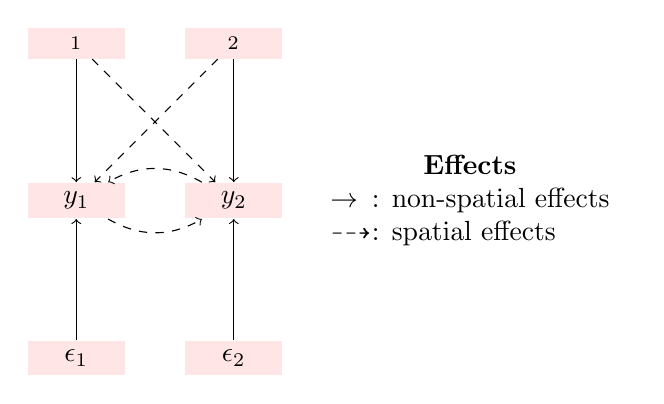
\begin{tikzpicture}
			\node[rectangle, text  width = 1cm, fill = red!10, align = center] (y1) at (-1,0) {$y_1$};
			\node[rectangle, text  width = 1cm, fill = red!10, align = center] (x1) at (-1,2) {$\vx_1$};
			\node[rectangle, text  width = 1cm, fill = red!10, align = center] (e1) at (-1,-2) {$\epsilon_1$};
			\node[rectangle, text  width = 1cm, fill = red!10, align = center] (y2) at (1, 0) {$y_2$};
			\node[rectangle, text  width = 1cm, fill = red!10, align = center] (x2) at (1,2) {$\vx_2$};
			\node[rectangle, text  width = 1cm, fill = red!10, align = center] (e2) at (1,-2) {$\epsilon_2$};

			\draw[->, solid] (x1) to (y1);
			\draw[->, solid] (x2) to (y2);
			\draw[->, solid] (e1) to (y1);
			\draw[->, solid] (e2) to (y2);
			\draw[dashed, ->] (y1) to[bend right] (y2);
			\draw[dashed, ->] (y2) to[bend right] (y1);
			\draw[dashed, ->] (x1) to (y2);
			\draw[dashed, ->] (x2) to (y1);
			%\draw[->, solid] (0,-4) to node[right, align = center] {$\sigma_i = 1$} (6,-5.4);
			%\draw[->, solid] (-6,-6.6) to node[right] {$\sigma_i = \sigma = 1$} (-2.5,-8);
			%\draw[->, solid] (6,-6.6) to node[right] {$\var(\veta_i)=\vzeros$} (2.5,-8);
			
			% Legend
       \node (leyend) at (4, 0){
    \begin{tabular}{l@{: }l}
      \multicolumn{2}{c}{\textbf{Effects}}              \\
      $\rightarrow$                        & non-spatial effects    \\
      $\dashrightarrow$                     & spatial effects  \\
      \end{tabular}
      };
		\end{tikzpicture}
\end{figure}

As an example, consider that $y$ is some measure of air pollution in each region. Thus, $\mW\vy$ states that air pollution in region  1 might affect pollution in region 2, and vice versa. If $\mX$ contains a measure of population density, the variable $\mW\mX$ would indicate that density and region 1 (2) would affect air pollution in region 2 (1). 

This model has also very good properties in terms of calculation of marginal effects that will explore later. 

% This model have very good properties \citep[see for example][]{lesage2010introduction,elhorst2010applied}. The strengths of this model are the following:
% 
% \begin{enumerate}
% 	\item SDM produces unbiased coefficient estimates also if the true data-generation process is a spatial lag or spatial error model.
% 	\item It  does not impose prior restrictions on the magnitude of potential spatial spillover effects. 
% 	\item In contrast to other spatial regression specifications, these spillovers effects can be global or local and be different for different explanatory variables.  
% \end{enumerate}

%====================================
\subsection{Spatial Error Model}\label{sec:tax_SEM}
%====================================

Another form of spatial dependence occurs when the dependence works through the error process, in that the errors from different areas may display spatial autocorrelation. The Spatial Error Model (SEM) is formulated as\index{Spatial error model}:

\begin{equation}\label{eq:sem_model_comp}
  \begin{aligned}
\vy &= \alpha \vones + \mX\vbeta + \vu, \\
\vu &= \lambda \mW\vu + \vepsi. \\
 \end{aligned}
\end{equation}
%
where $\lambda$ is the autoregressive parameter for the error lag $\mW\vu$ (to distinguish the notation from the spatial autoregressive coefficient $\rho$ in a spatial lag model), and $\vepsi$ is a generally a i.i.d noise. Figure \ref{figure:sem} visualizes the SEM for two regions. Note that the error term of both regions are related, and the only spatial effect goes from $\epsilon_1$ to $\epsilon_2$ and vice versa. 	

\begin{figure}[ht]
	\centering
	\caption{The SEM for two regions}\label{figure:sem}	
		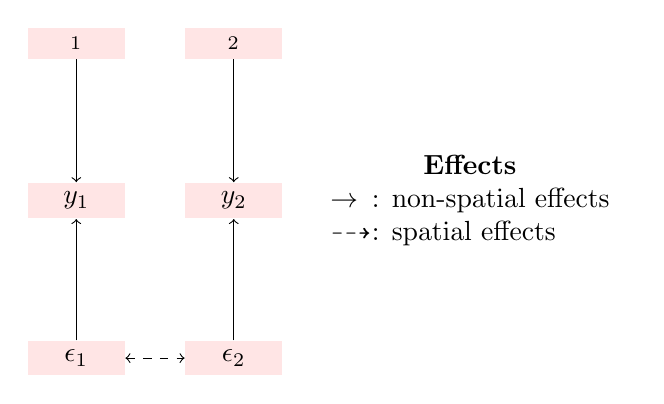
\begin{tikzpicture}
			\node[rectangle, text  width = 1cm, fill = red!10, align = center] (y1) at (-1,0) {$y_1$};
			\node[rectangle, text  width = 1cm, fill = red!10, align = center] (x1) at (-1,2) {$\vx_1$};
			\node[rectangle, text  width = 1cm, fill = red!10, align = center] (e1) at (-1,-2) {$\epsilon_1$};
			\node[rectangle, text  width = 1cm, fill = red!10, align = center] (y2) at (1, 0) {$y_2$};
			\node[rectangle, text  width = 1cm, fill = red!10, align = center] (x2) at (1,2) {$\vx_2$};
			\node[rectangle, text  width = 1cm, fill = red!10, align = center] (e2) at (1,-2) {$\epsilon_2$};

			\draw[->, solid] (x1) to (y1);
			\draw[->, solid] (x2) to (y2);
			\draw[->, solid] (e1) to (y1);
			\draw[->, solid] (e2) to (y2);
			\draw[dashed, <->] (e1) to (e2);

			% Legend
       \node (leyend) at (4, 0){
    \begin{tabular}{l@{: }l}
      \multicolumn{2}{c}{\textbf{Effects}}              \\
      $\rightarrow$                        & non-spatial effects    \\
      $\dashrightarrow$                     & spatial effects  \\
      \end{tabular}
      };
		\end{tikzpicture}
\end{figure}

As stated by \cite{AnselinBera1998}, spatial error dependence may be interpreted as a nuisance (and the parameter $\lambda$ as a nuisance parameter) in the sense that it reflects spatial autocorrelation in measurement errors or in variables that are otherwise not crucial to the model (i.e., the ``ignored'' variables spillovers across the spatial units of observations). 

Unlike previous models, interactions effects among the error terms do not require a theoretical model for a spatial or social interaction process, but instead, are consistent with a situation where determinants of the dependent variable omitted from the model are spatially autocorrelated, or with a situation where unobserved shocks follows a spatial pattern. 

The spatial diffusion of this model can be analyzed if we consider the reduced form equation. If the matrix $(\mI_n - \lambda\mW)$ is not singular, then \eqref{eq:sem_model_comp} can be written under the following reduced form\index{Spatial error model!reduced form}:

\begin{equation}
  \vy =  \alpha \vones + \mX\vbeta + (\mI_n - \lambda\mW)^{-1}\vepsi.
\end{equation}

This expression leads to a global spatial diffusion effect, but there is not spatial multiplier effect. The variance-covariance matrix is given by:

\begin{equation}
  \begin{aligned}
\E\left(\left.\vy\vy^\top\right|\mW, \mX\right)  & = \E\left(\left.\vepsi\vepsi^\top\right|\mW, \mX\right) \\
                 & = \left(\mI_n- \lambda\mW\right)^{-1}\E\left(\left.\vepsi\vepsi^\top\right|\mW, \mX\right)\left(\mI_n- \lambda\mW^\top\right)^{-1}
\end{aligned}
\end{equation}

\begin{remark}
Interaction effects among the unobserved terms may also be interpreted to reflect a mechanism to correct rent-seeking politicians for unanticipated fiscal policy changes. See for example \cite{allers2005tax}.
\end{remark}

%=========================
\subsection{Spatial Autocorrelation Model}
%=========================

A more general model is the one that includes the key modeling insights from both spatial lag and spatial error model describe above.  This model is called the Spatial Autocorrelation Model (SAC) and the its structural representation is the following:

\begin{equation*}
  \begin{aligned}
    y_i & = \alpha + \rho    \sum_{j = 1}^n w_{ij} y_j + \sum_{k=1}^K x_{ik}\beta_k + u_i \\
    u_i & = \lambda \sum_{j = 1}^n m_{ij} u_j + \epsilon_i
  \end{aligned}
\end{equation*}
%
or more compactly, 

\begin{equation}
  \begin{aligned}
\vy &= \alpha \vones_n + \rho \mW\vy + \mX\vbeta + \vu \\
\vu &= \lambda \mM\vu + \vepsi \\
  \end{aligned}
\end{equation}
%
where the matrix $\mW$ and $\mM$ are $n\times n$ spatial-weighting matrices.\footnote{This model is also known as SARAR(1, 1) model or Cliff-Ord models because of the impact that \cite{cliff1973spatial}  had on the subsequent literature. Note that SARAR(1, 1) is  a special case of the more general SARAR(p, q) model.} In this model, spatial interactions in the dependent variable and the disturbances are considered. As standard, the spatial weight matrices $\mW$ and $\mM$ are taken to be known and nonsthocastic. These matrices are part of the model definition, and in many applications, $\mM = \mW$. When $\rho = 0$, the model reduces to the SEM. When $\lambda = 0$ the model reduces to the SLM (SAR) specification. Setting $\rho = 0$ and $\lambda = 0$ causes the model to reduce to a linear regression model with exogenous variables. 

The reduced form is given by:

\begin{equation}
\vy = \left(\mI_n - \rho \mW\right)^{-1}\left(\mX\vbeta + \alpha \vones_n\right) + \left(\mI_n - \rho\mW\right)^{-1}\left(\mI_n - \rho \mM\right)^{-1}\vepsi.
\end{equation}

Figure \ref{fig:taxonomy} gives a more complete taxonomy for different spatial models. The more complete model is the General Nesting Spatial Model (GNS or Manski's Model), which includes spatial dependence in the dependent variable, exogenous variables and the error term. Different restrictions give rise to different spatial models. 


\begin{figure}[h]
\caption{Taxonomy of spatial models}
\label{fig:taxonomy}
\centering
\begin{tikzpicture}[scale = 0.8]
			\node[rectangle, text  width = 5cm, fill = red!10, align = center] (gns) at (0,0) {\scriptsize General nesting spatial model \\
			\begin{eqnarray*}
			\vy &=& \rho\mW\vy + \mX\vbeta + \mW\mX\vgamma + \vu \\
			\vu &=& \lambda\mW\vu + \vepsi
			\end{eqnarray*}};
			
			\node[rectangle, text  width = 3cm, fill = red!10, align = center] (sac) at (6,4) {\scriptsize  SAC \\
			\begin{eqnarray*}
			\vy &=& \rho\mW\vy + \mX\vbeta + \vu \\
			\vu &=& \lambda\mW\vu + \vepsi
			\end{eqnarray*}};
			
			\node[rectangle, text  width = 3cm, fill = red!10, align = center] (sdm) at (6,0) {\scriptsize  Spatial durbin model \\
			\begin{equation*}
			\vy = \rho\mW\vy + \mX\vbeta + \mW\mX\vgamma + \vepsi
			\end{equation*}};
			
			\node[rectangle, text  width = 3cm, fill = red!10, align = center] (sde) at (6,-4) {\scriptsize Spatial durbin error model \\
			\begin{eqnarray*}
			\vy &=& \mX\vbeta + \mW\mX\vgamma + \vu \\
			\vu &=& \lambda\mW\vu + \vepsi
			\end{eqnarray*}};
			
			\node[rectangle, text  width = 3cm, fill = red!10, align = center] (slm) at (12,4) {\scriptsize Spatial Lag Model \\
			\begin{equation*}
			\vy = \rho\mW\vy + \mX\vbeta + \vepsi
			\end{equation*}};
			
			\node[rectangle, text  width = 3cm, fill = red!10, align = center] (slx) at (12,0) {\scriptsize SLX \\
			\begin{equation*}
			\vy = \mX\vbeta + \mW\mX\vgamma + \vepsi
			\end{equation*}};
			
			\node[rectangle, text  width = 3cm, fill = red!10, align = center] (sem) at (12,-4) {\scriptsize Spatial error model \\
			\begin{eqnarray*}
			\vy &=& \mX\vbeta + \vu \\
			\vu &=& \lambda\mW\vu + \vepsi
			\end{eqnarray*}};
			
			\node[rectangle, text  width = 2cm, fill = red!10, align = center] (ols) at (16,0) {\scriptsize OLS \\
			\begin{equation*}
			\vy = \mX\vbeta + \vepsi
			\end{equation*}};

			\draw (gns) -- (sac) node [->, solid, midway, above, sloped] {\scriptsize $\vgamma = 0$};
			\draw (gns) -- (sdm) node [->, solid, midway, above, sloped] {\scriptsize $\lambda = 0$};
			\draw (gns) -- (sde) node [->, solid, midway, above, sloped] {\scriptsize $\rho = 0$};
			\draw (sac) -- (slm) node [->, solid, midway, above, sloped] {\scriptsize $\lambda = 0$};
			\draw (sac) -- (sem) node [->, solid, near end, above, sloped] {\scriptsize $\rho = 0$};
			\draw (sdm) -- (slx) node [->, solid, near end, above, sloped] {\scriptsize $\rho = 0$};
			\draw (sde) -- (slx) node [->, solid, near start, above, sloped] {\scriptsize $\lambda = 0$};
			\draw (sdm) -- (slm) node [->, solid, midway, above, sloped] {\scriptsize $\gamma = 0$};
			\draw (sdm) -- (sem) node [->, solid, midway, above, sloped] {\scriptsize $\gamma = -\rho\beta$};
			\draw (sde) -- (sem) node [->, solid, midway, above, sloped] {\scriptsize $\gamma = 0$};
			\draw (slm) -- (ols) node [->, solid, midway, above, sloped] {\scriptsize $\rho = 0$};
			\draw (slx) -- (ols) node [->, solid, midway, above, sloped] {\scriptsize $\gamma = 0$};
			\draw (sem) -- (ols) node [->, solid, midway, above, sloped] {\scriptsize $\lambda = 0$};
			%\draw[->, solid] (x2) to (y2);
			%\draw[->, solid] (e1) to (y1);
			%\draw[->, solid] (e2) to (y2);
			%\draw[dashed, <->] (e1) to (e2);

			% Legend
     %  \node (leyend) at (4, 0){
    %     \begin{tabular}{l@{: }l}
    %  \multicolumn{2}{c}{\textbf{Effects}}              \\
    %  $\rightarrow$                        & non-spatial effects    \\
    %  $\dashrightarrow$                     & spatial effects  \\
    %  \end{tabular}
    %  };
\end{tikzpicture}
\end{figure}

Starting with the GNS model:

\begin{itemize}
  \item Imposing the restriction $\vgamma = \vzeros$ leads to the SAC model that includes both a spatial lag for the dependent variable and spatial lag for the error term, but excludes the influence of the spatially lagged explanatory variables. 
  \item Imposing the restriction $\lambda = 0$ leads to the SDM.
  \item Imposing the restriction $\rho = 0$ leads to the Spatial Durbin Error Model (SDEM). 
\end{itemize}

Starting with the SDM:

\begin{itemize}
  \item The so-called common factor parameter restrictions $(\vgamma = -\rho\vbeta)$ yields the spatial error regression model (SEM) specification that assumes that externalities across spatial unites are mostly a nuisance spatial dependence problem caused by the regional transmission of random shocks. 
  \item Imposing the restriction $\gamma = 0$ leads to the spatial lag model (SLM), whereas the restriction $\rho = 0$ results in a least-squares spatially lagged $\mX$ regression model (labeled SLX) that assumes independence between regions in the dependent variable, but includes characteristics from neighboring regions in the form of spatially lagged explanatory variables.  
\end{itemize}

Finally, if $\rho = \lambda = 0$ and $\vtheta = 0$, then we obtain the traditional linear regression model. 

%==============================================
\section{Motivation of Spatial Models}\label{sec:motivation}
%==============================================

\subsection{SLM as a Long-run Equilibrium}\label{sec:SLM_lre}

It can be shown that a SLM can be considered as a simultaneous dependence system over time that culminate in a new steady state equilibrium, even using a cross-sectional dataset.

To illustrate this, consider $\vy_t$, which represent some dependent variable vector at time $t$. Assume that this variable is determined by a spatial autoregressive scheme that depends on space-time lagged values of the dependent variable from neighboring observations. This would lead to a time lag of the average neighboring values of the dependent variable observed during previous period,  $\mW\vy_{t-1}$. We can also include current period own-region characteristics $\mX_t$ in the model. If the characteristics of regions remain relatively fixed over time, we can write $\mX_t = \mX$ As an illustration, consider a model involving pollution as the dependent variable $\vy_t$, which depend on past period pollution of neighboring regions, $\mW\vy_{t-1}$. Then, the more appropriate process is the following:

\begin{equation}\label{eq:slm_with_time}
\vy_t = \rho \mW\vy_{t-1} + \mX\vbeta + \vepsi_t.
\end{equation}

Note that we can replace $\vy_{t-1}$ on the right-hand side of (\ref{eq:slm_with_time}) with:

\begin{equation*}
\vy_{t-1} = \rho \mW\vy_{t-2} + \mX\vbeta + \vepsi_{t-1},
\end{equation*}
%
producing:

\begin{equation}\label{eq:recur_2}
\begin{aligned}
\vy_t  = & \mX\vbeta +\rho\mW\left(\mX\vbeta + \rho \mW\vy_{t-2} + \vepsi_{t-1}\right) + \vepsi_t\\
=& \mX\vbeta +\rho\mW\mX\vbeta + \rho^2\mW^2\vy_{t-2} + \epsilon_t + \rho\mW\vepsi_{t-1}.
\end{aligned}
\end{equation}

Recursive substitution for past values of the vector $\vy_{t-r}$ on the right-hand side of (\ref{eq:recur_2}) over $q$ periods leads to:

\begin{equation*}
  \begin{aligned}
    \vy_t &= \left(\mI_n + \rho\mW + \rho^2\mW^2 + ... + \rho^{q-1}\mW^{q-1}\right)\mX\vbeta + \rho^q\mW^q\vy_{t-q} + \vu,\\
    \vu  & = \vepsi_{t} + \rho\mW\vepsi_{t-1} + \rho^2\mW^2\vepsi_{t-2} + ... + \rho^{q-1}\mW^{q-1}\vepsi_{t - (q-1)}. 
  \end{aligned}
\end{equation*}

The expected value of this spatial process is:

\begin{equation}\label{eq:expectation_time}
  \E\left(\vy_t\right) = \left(\mI_n + \rho\mW + \rho^2\mW^2 + ... + \rho^{q-1}\mW^{q-1}\right)\mX\vbeta + \rho^q\mW^q\vy_{t-q},
\end{equation}
%
where we use the fact that $\E(\vepsi_{t-r}) = 0, r = 0, ..., q-1$, which also implies that $\E(\vu) = \vzeros$. Finally, taking the limit of \eqref{eq:expectation_time}, 

\begin{equation}\label{eq:steady_state}
\lim_{q\to \infty} \E\left(\vy_t\right) = \left(\mI_n - \rho\mW\right)^{-1}\mX\vbeta.
\end{equation}
%
Note that we use the fact that the magnitude of $\rho^q\mW^q\vy_{t-q}$ tends to zero for large $q$, under the assumption that $\lvert \rho \rvert <1$ and assuming that $\mW$ is row-stochastic, so the matrix $\mW$ has a principal eigenvalue of 1. 

Equation (\ref{eq:steady_state}) states that we can interpret the observed cross-sectional relation as the outcome or expectation of a long-run equilibrium or steady state. Note that this provides a dynamic motivation for the data generating process of the cross-sectional SLM that serves as a \textbf{workhorse} of spatial regression modeling. That is, a cross-sectional SLM relation can arise from time-dependence of decisions by economic agents located at various point in space when decisions depend on those neighbors. 



\subsection{SEM and Omitted Variables Motivation}

Consider the following process:

\begin{equation*}
\vy = \vx\beta + \vz\theta,
\end{equation*}
%
where $\vx$ and $\vz$ are \textbf{uncorrelated} vectors of dimension $n\times 1$, and the vector $\vz$ follows the following spatial autoregressive process:

\begin{eqnarray*}
  \vz &=& \rho \mW\vz + \vr \\
  \vz &=& \left(\mI_n - \rho\mW\right)^{-1}\vr
\end{eqnarray*}
%
where $\vr \sim \rN(0, \sigma^2_{\epsilon}\mI_n)$. Examples of $\vz$ are culture, social capital, or neighborhood prestige. 

If $\vz$ is not observed, then:


\begin{equation}\label{eq:sem_omited_moti}
  \begin{aligned}
    \vy & = \vx\beta + \vu \\
    \vu & = \left(\mI_n - \rho\mW\right)^{-1}\vepsi
  \end{aligned}
\end{equation}
%
where $\vepsi = \theta\vr$. Then, we have the DGP for the SEM.

\subsection{SDM and Omitted Variables Motivation}

Now suppose that $\mX$ and $\vepsi$ from (\ref{eq:sem_omited_moti}) are correlated, given by the following process:

\begin{equation}\label{eq:cor_x_epsi}
\begin{aligned}
  \vepsi & = \vx \gamma + \vv \\
  \vv    & \sim \rN(0, \sigma^2\mI_n) 
\end{aligned}
\end{equation}
%
where the scalar parameters $\gamma$ and $\sigma^2$ govern the strength of the relationship between $\mX$ and $\vz = (\mI_n-\rho\mW)^{-1}\vr$. Inserting (\ref{eq:cor_x_epsi}) into (\ref{eq:sem_omited_moti}), we obtain:

\begin{equation}
  \begin{aligned}
    \vy & = \vx\beta + \left(\mI_n - \rho\mW\right)^{-1}\vepsi \\
        & = \vx\beta + \left(\mI_n - \rho\mW\right)^{-1}\left(\vx \gamma + \vv\right) \\
        & = \vx\beta + \left(\mI_n - \rho\mW\right)^{-1}\vx \gamma + \left(\mI_n - \rho\mW\right)^{-1}\vv \\
       \left(\mI_n - \rho\mW\right)\vy & = \left(\mI_n - \rho\mW\right)\vx\beta  + \vv \\
       \vy & = \rho\mW\vy + \vx\left(\beta + \gamma\right) + \mW\vx(-\rho\beta) + \vv
  \end{aligned}
\end{equation}

This is the Spatial Durbin Model (SDM), which includes a spatial lag of the dependent variable $\vy$, as well as the explanatory variables $\vx$.


%==============================================
\section{Interpreting Spatial Models}\label{sec:interpretation}
%==============================================

\subsection{Measuring Spillovers}

A major focus of regional science is measuring spatial spillover. A basic definition of spillovers in a spatial context would be that changes occurring in one region exert impacts on other regions \citep{LeSage2014}. Some examples are:

\begin{itemize}
  \item Changes in tax rate by one spatial unit might exert an impact on tax rate setting decisions of nearby regions, a phenomenon that has been labeled tax mimicking and yardstick competition between local government. 
  \item Situations where home improvements made by one homeowner exert a beneficial impact on selling prices of neighboring homes.
  \item Innovation by university researchers diffuses to nearby firms.
  \item Air or water pollution generated in one region spills over to nearby regions. 
\end{itemize}

The models reviewed in the previous section can be use to formally define the concept of a spatial spillover and,  more importantly, to provide estimates of the quantitative magnitude of spillovers and test their statistical significance.  There is however a distinction between global and local spillovers, which is discussed in \cite{anselin2003spatial} and \cite{LeSage2014}. 

We start our discussion about spillovers by formally defining global spillovers. 

\begin{definition}[Global Spillovers]\index{Spillover effects!Global spillovers}
	 Global spillovers arise when changes in a characteristic of one region impact all regions' outcomes. This applies even to the region itself since impacts can pass to the neighbors and back to the own region (feedback). Specifically, global spillovers impact the neighbors, neighbors to the neighbors, neighbors to the neighbors to the neighbors and so on. 
\end{definition}

The endogenous interactions produced by global spillovers lead to a scenario where changes in one region set in motion a sequence of adjustments in (potentially) all regions in the sample such that a new long-run steady state equilibrium arises \citep{lesage2014regional}.

As explained by \cite{lesage2014regional}, global spillovers might arise when considering local policies interactions. For example: \emph{``it seems plausible that changes in levels of public assistance (cigarette taxes) in state $A$ would lead to a reaction by neighboring states $B$ to change their levels of assistances (taxes), which in turn produces a game-theoretic (feedback) response of state $A$, and also responses of states $C$ who are neighbors to neighboring states $B$, and so on.''}


The following definition corresponds to local spillovers.

 \begin{definition}[Local Spillovers]\index{Spillover effects!Local spillovers}
 	Local spillovers represent a situation where the impact fall only on nearby or immediate neighbors, dying out before they impact regions that are neighbors to the neighbors.
 \end{definition}	

As it can be noted from the previous definitions, the main difference is that feedback or endogenous interaction is only possible for global spillovers. 

%\begin{remark}
%According to \cite{anselin2003spatial} and \cite{LeSage2014}, different spatial models give rise to different measures of spillovers.
%\end{remark}


\subsection{Marginal Effects}\index{Spillover effects!Marginal effects}

Mathematically, the notion of spillover can be thought as the derivative $\partial y_i/ \partial x_j$. This means that changes to explanatory variables in region $i$ impact the dependent variable in region $j\neq i$.

As an illustration, consider the SDM model, which can be re-written as:

\begin{equation*}
\begin{aligned}
(\mI_n - \rho\mW)\vy & = \mX\vbeta + \mW\mX\vtheta + \vepsi, \\
\vy & =   (\mI_n - \rho\mW)^{-1}\mX\vbeta + (\mI_n - \rho\mW)^{-1}\mW\mX\vtheta + (\mI_n - \rho\mW)^{-1}\vepsi, \\
\vy & =   \mA(\mW)^{-1}\mX\vbeta + \mA(\mW)^{-1}\mW\mX\vtheta + \mA(\mW)^{-1}\vepsi,\quad \mbox{since $\mA(\mW) = (\mI_n - \rho\mW)^{-1}$}\\
\vy & =   \mA(\mW)^{-1}\left(\mX\vbeta + \mW\mX\vtheta\right) + \mA(\mW)^{-1}\vepsi, \\
\vy & =   \sum_{r=1}^K\mA(\mW)^{-1}\left(\mI_n\beta_r + \mW\theta_r\right)\vx_r + \mA(\mW)^{-1}\vepsi, \\
\underbrace{\vy}_{(n\times 1)} & =   \sum_{r=1}^K\underbrace{\mS_r(\mW)}_{(n\times n)}\underbrace{\vx_r}_{n\times 1} + \underbrace{\mA(\mW)^{-1}}_{(n\times n)}\underbrace{\vepsi}_{n\times 1}
\end{aligned}
\end{equation*}
%
where $\mS_r = \mA(\mW)^{-1}\left(\mI_n\beta_r + \mW\theta_r\right)$, and

\begin{equation*}
 \vx_r = \begin{pmatrix}
          x_{r1} \\
          x_{r2} \\
          \vdots \\
          x_{rn}
        \end{pmatrix}.
\end{equation*}

Assuming that $\E(\epsilon_i) = 0$, then the expansion of the expected value yields:

\begin{equation}\label{eq:system_expected}
\begin{pmatrix}
\E(y_1) \\ \E(y_2) \\ \vdots \\ \E(y_n)
\end{pmatrix}
=
\sum_{r=1}^K\begin{pmatrix}
\mS_r(\mW)_{11} & \mS_r(\mW)_{12} & \hdots & \mS_r(\mW)_{1n} \\
\mS_r(\mW)_{21} & \mS_r(\mW)_{22} & \hdots & \mS_r(\mW)_{2n} \\
\vdots & \vdots & \ddots & \vdots \\ 
\mS_r(\mW)_{n1} & \mS_r(\mW)_{n2} & \hdots & \mS_r(\mW)_{nn} 
\end{pmatrix}
\begin{pmatrix}
x_{1r} \\ x_{2r} \\ \vdots \\ x_{nr} 
\end{pmatrix}.
\end{equation}

For the dependent variable for spatial unit $i$, Equation (\ref{eq:system_expected}) would be:

\begin{equation}
\E(y_i) = \sum_{r=1}^k\left[\mS_r(\mW)_{i1}x_{1r} + \mS_r(\mW)_{i2}x_{2r} + ... + \mS_r(\mW)_{in}x_{nr}\right].
\end{equation}

So, the impact on the expected value of location $i$ given a change in the explanatory variable $x_r$ in location $j$ is\index{Spillover effects!Indirect effects}

\begin{equation}\label{eq:indirect_impact}
\frac{\partial \E(y_i)}{\partial x_{jr}} = \mS_r(\mW)_{ij}
\end{equation}
%
where $\mS_r(\mW)_{ij}$ is this equation represents the $i,j$th element of the matrix $\mS_r(\mW)$. This result implies that, unlike the OLS model, a change in some variable in certain region will potentially affect the expected value of the dependent variable in all other regions. Given this characteristic, this type of effect is known as \textbf{indirect effect}.

The impact of the expected value of region $i$, given a change in certain variable for the same region is given by\index{Spillover effects!Direct effects}

\begin{equation}\label{eq:direct_impact}
\frac{\partial \E(y_i)}{\partial x_{ir}} = \mS_r(\mW)_{ii}.
\end{equation}

This impact includes the \textbf{effect of feedback loops} where observation $i$ affects observation $j$ and observation $j$ also affects observation $i$: a change in $x_{ir}$ will affect the expected value of dependent variable in $i$, then will pass through the neighbors of $i$ and back to the region itself. To shed more light on this, let us write the all the marginal effects in matrix notation as follows:

\begin{equation}\label{eq:matrix_marginal_effects}
\begin{aligned}
 \underset{(n \times n)}{\begin{pmatrix}
  \frac{\partial \E(\vy)}{\partial x_{1r}} & \frac{\partial \E(\vy)}{\partial x_{2r}} & \hdots & \frac{\partial \E(\vy)}{\partial x_{nr}} 
   \end{pmatrix}} & = 
  \begin{pmatrix}
  \frac{\partial \E(y_1)}{\partial x_{1r}} & \frac{\partial \E(y_1)}{\partial x_{2r}} & \hdots & \frac{\partial \E(y_1)}{\partial x_{nr}} \\
  \frac{\partial \E(y_2)}{\partial x_{1r}} & \frac{\partial \E(y_2)}{\partial x_{2r}} & \hdots & \frac{\partial \E(y_2)}{\partial x_{nr}} \\
  \vdots & \vdots & \ddots & \vdots \\
  \frac{\partial \E(y_n)}{\partial x_{1r}} & \frac{\partial \E(y_n)}{\partial x_{2r}} & \hdots & \frac{\partial \E(y_n)}{\partial x_{nr}} 
  \end{pmatrix} \\
  & = \mA(\mW)^{-1}\left(\mI_n\beta_r + \mW\theta_r\right) = \mS_r(\mW) \\
  & = (\mI_n - \rho\mW)^{-1}
  \begin{pmatrix}
    \beta_r  & w_{12} \theta_r  & \hdots & w_{1n}\theta_r \\
    w_{21} \theta_r  & \beta_r   & \hdots & w_{2n}\theta_r \\
    \vdots & \vdots & \ddots & \vdots \\
    w_{n1} \theta_r  & w_{n2} \theta_r  & \hdots  & \beta_r \\
  \end{pmatrix}
\end{aligned}  
\end{equation}

This expression is somewhat difficult to understand. To provide a better understanding we follow \cite{elhorst2010applied} and consider a model with 3 regions arranged linearly\footnote{Unit 1 is neighbor of unit 2, unit 2 is a neighbor of both units 1 and 3, and unit 3 is a neighbor of unit 2.} with the following matrices:

\begin{equation}\label{eq:w_mat_ex_spill}
  \mW = \begin{pmatrix}
          0      & 1 & 0 \\
          w_{21} & 0 & w_{23} \\
          0      & 1 & 0
        \end{pmatrix}
\end{equation}
%
and

\begin{equation}\label{eq:w_Imat_ex_spill}
  \mA(\mW)^{-1} = \frac{1}{1 - \rho^2}
  \begin{pmatrix}
          1 - w_{23}\rho^2     & \rho & \rho^2 w_{23}\\
          \rho w_{21} & 1 & \rho w_{23} \\
          \rho^2 w_{21}      & \rho & 1 - w_{21}\rho^2 
        \end{pmatrix}
\end{equation}
%
where $w_{12} = w_{31}= 1$ since units 1 and 3 have only one neighbor, and $w_{21} + w_{23} = 1$, so we explicitly consider a row-standardized matrix.  Substituting Equations (\ref{eq:w_mat_ex_spill}) and (\ref{eq:w_Imat_ex_spill}) into Equation (\ref{eq:matrix_marginal_effects}) we get:

\begin{equation*}
  \begin{pmatrix}
  \frac{\partial \E(\vy)}{\partial x_{1r}} & \frac{\partial \E(\vy)}{\partial x_{2r}} & \frac{\partial \E(\vy)}{\partial x_{3r}} 
   \end{pmatrix} = \frac{1}{1 - \rho^2}
   \begin{pmatrix}
    \left(1 -  w_{23}\rho^2\right)\beta_r + \left(w_{21}\rho\right) \theta_r & \rho \beta_r + \theta_r & \left(w_{23}\rho^2\right)\beta_r + (\rho w_{23})\theta_r \\
    (w_{21}\rho)\beta_r + w_{21}\theta_r & \beta_r + \rho \theta_r & (w_{23}\rho)\beta_r + w_{23}\theta_r \\
    (w_{21}\rho^2)\beta_r + (w_{21}\rho)\theta_r & \rho \beta_r + \theta_r & (1 -  w_{21}\rho^2)\beta_r + (w_{23}\rho)\theta_r
   \end{pmatrix}
\end{equation*}

Every diagonal element of this matrix represents a direct effect. Consequently, indirect effect do not occur if both $\rho = 0$ and $\theta_k = 0$, since all non-diagonal elements will then be zero. Another important insight is that direct and indirect effects are different for different spatial units in the sample. Direct effects are different because the diagonal elements of the matrix $(\mI_n - \rho\mW)^{-1}$ are different for different units, provided that $\rho \neq 0$. Indirect effects are different because both the non-diagonal elements of the matrix $(\mI_n - \rho\mW)^{-1}$ and of the matrix $\mW$ are different for different units, provided that $\rho \neq 0$ and/or $\theta_k\neq 0$. Finally, note that indirect effects that occur if $\theta_k\neq 0$ are \textbf{local effects}, whereas indirect effects that occur if $\rho\neq 0$ are \textbf{global effects}. 


\subsubsection{Summary Measures}\label{sec:summary-measures}

In general, the change of each variable in each region implies $n^2$ potential marginal effects.  If we have $K$ variables in our model, this implies $K\times n^2$ potential measures. Even for small values of $n$ and $K$, it may already be rather difficult to report these results compactly. To overcome this problem, \citet[][p. 36-37]{lesage2010introduction} propose the following scalar summary measures: 

\begin{definition}[Average Direct Impact]\label{def:ADI}
Let $\mS_r = \mA(\mW)^{-1}\left(\mI_n\beta_r + \mW\theta_r\right)$ for variable $r$. The impact of changes in the $i$th observation of $x_r$, which is denoted $x_{ir}$, on $y_i$ could be summarized by measuring the average $S_r(\mW)_{ii}$, which equals
	
	\begin{equation}
		\mbox{ADI} = \frac{1}{n}\tr\left(\mS_r(\mW)\right)
	\end{equation}
\end{definition}


Averaging over the direct impact associated with all observations $i$ is similar in spirit to typical regression coefficient interpretations that represent average response of the dependent to independent variables over the sample of observations. 	

\begin{definition}[Average Total Impact to an Observation]\label{def:ATIT}
	Let $\mS_r = \mA(\mW)^{-1}\left(\mI_n\beta_r + \mW\theta_r\right)$ for variable $r$. The sum across the $i$th row of $\mS_r(\mW)$ would be represent the total impact on individual observation $y_i$ resulting from changing the $r$th explanatory variable by the same amount across all $n$ observations. There are $n$ of these sums given by the column vector $\vc_r = \mS_r(\mW)\vones_n$, so an average of these total impacts is:
		\begin{equation}
		\mbox{ATIT} = \frac{1}{n} \vones_n'\vc_r
		\end{equation} 
\end{definition}

\begin{definition}[Average Total Impact from an Observation]\label{def:ATIF}
	Let $\mS_r = \mA(\mW)^{-1}\left(\mI_n\beta_r + \mW\theta_r\right)$ for variable $r$. The sum down the $j$th column of $\mS_r(\mW)$ would yield the total impact over all $y_i$ from changing the $r$th explanatory variable by an amount in the $j$th observation. There are $n$ of these sums given by the row vector $\vr_r = \vones_n'\mS_{r}(\mW)$, so an average of these total impacts is:
				\begin{equation}
				\mbox{ATIF} = \frac{1}{n} \vr_r\vones_n
				\end{equation} 
\end{definition}

The definition \ref{def:ATIF} relates how changes in a single observation $j$ influences all observations. In contrast, definition \ref{def:ATIT} considers how changes in all observations influences a single observation $i$. In both cases, averaging over all $n$ observations, leads to the same numerical result. The implication of this interesting result is that the \textbf{average total impact} is the average of all derivatives of $y_i$ with respect to $x_{jr}$ for any $i, j$. 

Therefore:

\begin{eqnarray}
\bar{M}(r)_{\mbox{direct}} & = & n^{-1}\tr\left(\mS_r(\mW)\right) \\
\bar{M}(r)_{\mbox{total}} & = & n^{-1}\vones_n'\mS_r(\mW)\vones_n \\
\bar{M}(r)_{\mbox{indirect}} & = & \bar{M}(r)_{\mbox{total}} - \bar{M}(r)_{\mbox{direct}}
\end{eqnarray}	


Given our example above, we obtain a direct effect of:

\begin{equation*}
  \frac{(3- \rho^2)}{3(1 - \rho^2)}\beta_k + \frac{2p}{3(1-\rho^2)}\theta_k,
\end{equation*}
%
and an indirect effect of

\begin{equation*}
  \frac{3\rho + \rho^2}{(3(1-\rho^2))}\beta_k + \frac{3 + \rho}{3(1- \rho^2)}\theta_k.
\end{equation*}

Unfortunately, since every application will have its own unique number of observations $n$ and spatial weight matrix $(\mW)$, these formulae cannot be generalized. 


\begin{example}[The effect of number of workers on commuting times]\label{example:commuting-Kirby}
\cite{kirby2009changes} use an SDM specification to consider changes in the (logged) number of workers in the US census tracts with commuting times exceeding 45 minutes one way, between 1990 and 2000 (See also the example in Section \ref{sec:lesage-example}). The motivation of this investigation is the fact that the percentage of the US workers with these long commute times in 1990 was 12.5\% compared to 15.4\% in 2000, an increase of more than 10\%. When deciding which model to estimate, they note that spillover impacts from an increase in commuters traveling long distances to work would seem \textbf{global} in nature, since the congestion effects of more travelers on one segment of a metropolitan area roadway network impact travel times of other travelers on the entire network. Furthermore, they state that \textbf{feedback} effects seem likely since congestion arising from commuting decisions by workers in one tract will spillover to neighboring tracts, which in turn create congestion feedback to the own tract. These two observations led the authors to specify the following SDM:

\begin{equation*}
  \vy = \rho\mW\vy + \alpha \vones_n + \mX\vbeta + \mW\mX\vtheta + \vepsi,
\end{equation*}
%
where $\mX$ includes the (logged) number of workers with long commute times $(\vy)$, variables related to location decision of households; age, gender and income distribution of resident population, and geographical characteristics of the tract, and $\mW\mX$ includes these same characteristics of neighboring census tracts. 
Based on a comparison of \textbf{direct, indirect} and \textbf{total effects} estimates form the 1990 and 2000 models, they conclude that the suite of variables reflecting the age and gender distribution of population in the tracts represents the primary explanation for changes in the number of workers with long commute times between 1990 and 2000. The spillover impacts of the number of employed females in the 1990 model was positive suggesting that more employed females in a tract produced an increase in long commute times for neighboring tract commuters. In contrast, for the 2000 model, spillovers associated with employed females were negative, so that more employed females in a tract reduced long commute times for workers located in neighboring tracts. 
\end{example}


\begin{example}[Effect of pollution on housing price]\label{example:pollution-kim}
\cite{kim2003measuring} use a spatial-lag hedonic model in order to assess the direct and indirect effect of quality air on housing price.  The main model is the following:

\begin{equation*}
\vp = \rho\mW\vp + \mX_1\vbeta_1 + \mX_2\vbeta_2 + \mX_3\vbeta_3 + \vepsi,
\end{equation*}
%
where $\vp$ is the vector of housing prices, $\rho$ is a spatial autocorrelation parameter, $\mW$ is the $n\times n$ spatial weight matrix, $\mX_1$ is a matrix with observations on structural characteristics, $\mX_2$ is a matrix with observations on neighborhood characteristics, and $\mX_3$ is a matrix with observations on environmental quality (SO$_2$ and NO$_x$). 

The marginal implicit price (marginal benefit) of the hedonic equation is derived as

\begin{equation*}
\begin{pmatrix}
  \frac{\partial \E(\vp)}{\partial x_{1r}} & \frac{\partial \E(\vp)}{\partial x_{2r}} & \hdots & \frac{\partial \E(\vp)}{\partial x_{nr}} 
   \end{pmatrix} = \mA(\mW)^{-1}\mI_n\beta_r\quad \mbox{where}\quad \mA(\mW)^{-1} = (\mI_n - \rho\mW)^{-1}
\end{equation*}

Focusing on the first row the interpretation if the following: the housing price of location $i$ is not only affected by a marginal change air quality of location $i$ but also is affected by marginal changes of air quality in other locations. That is, the total impact of a change in air quality on housing price at location $i$ is the sum of the direct impacts $\partial p_1/\partial x_{1k}$ plus induced impacts $\sum_{i = 2}^n \partial p_1 / \partial x_{ik}$ (See our Definition \ref{def:ATIT}). 

An important point evidenced by \cite{kim2003measuring} is that, if  the row-sums of $\mW$ is less than or equal to one and $\rho$ in the proper parameter space, i.e., $\rho < 1$, then the total average effect can be computed as $\beta_r / (1-\rho)$. To see this note that

\begin{equation}\label{eq:total_effect_simple}
  \begin{aligned}
    n^{-1}\vones^\top\mS_r(\mW)\vones & = n^{-1}\vones^\top\left[\mA(\mW)^{-1}\left(\mI\beta_r\right)\right]\vones \\
                                  & = n^{-1}\vones^\top\left[(\mI_n - \rho\mW)^{-1}\right]\left(\mI\beta_r\right)\vones \\
                                  & =   n^{-1}\vones^\top\left[\mI_n + \rho\mW + \rho^2\mW^2 + ... \right]\left(\mI\beta_r\right)\vones \quad\mbox{using Lemma \ref{lemma:Leontief}} \\
                                  & = n^{-1} \vones^\top\left[\mI_n\beta_r + \rho\mW\beta_r + \rho^2\mW^2\beta_r + ... \right]\vones \\
                                  & = n^{-1} \vones^\top\left[\mI_n\vones\beta_r + \rho\mW\vones\beta_r + \rho^2\mW(\mW\vones)\beta_r + \rho^3\mW\mW(\mW\vones) \right] \\
                                  & = n^{-1} \vones^\top\left[\beta_r\vones + \rho\beta_r\vones + \rho^2\beta_r\vones + \rho^3\beta_r\vones + ... \right]\quad \because \mW^l\vones = \vones \\
                                  & = n^{-1} \vones^\top\left[\beta_r + \rho\beta_r + \rho^2\beta_r + \rho^3\beta_r + ... \right]\vones\\
                                  & = n^{-1} \left[\beta_r + \rho\beta_r + \rho^2\beta_r + \rho^3 + ... \right] \vones^\top\vones\\
                                  & = n^{-1} \left[\beta_r + \rho\beta_r + \rho^2\beta_r + \rho^3\beta_r + ... \right] n \\
                                  & = \frac{\beta_r}{(1 - \rho)}
  \end{aligned}
\end{equation}

The model is estimated in a semi-log functional form, therefore the estimated coefficients can be interpreted as semi-elasticities. In particular, note that the elasticity for SO$_2$ is given by:

\begin{equation}
  \begin{aligned}
    \epsilon_{SO_2} & = \left(\frac{SO_2}{p}\right)\left(\frac{d p}{d SO_2}\right) \\
                      & = \left(\frac{SO_2}{p}\right)\left(\frac{\beta_r}{(1 - \rho)}\cdot p\right)\quad \mbox{since the model is log-lin} \\
                      & = \frac{\beta_r}{(1 - \rho)}\cdot SO_2
  \end{aligned}
\end{equation}

Using the estimated $\widehat{\rho} =  0.549$ and replacing SO$_2$ by its mean value they obtain that the elasticity of housing price from a given small change in air quality is about $0.348 \approx 4\%$. The marginal benefits per household of a permanent 4\% improvement in air quality using $\beta_{SO_2}(\mI_n - \rho\mW)^{-1}\vp$ is about \$2333 (1.43\% of mean house value) for owners. 
\end{example}

\begin{example}[Human capital and labor productivity]
\cite{fischer2009impact} analyze the role of human capital in explaining labor productivity variation among European region. In particular they estimate the following model:

\begin{equation*}
\vy = \rho\mW\vy + \mX\vbeta + \mW\mX\vgamma +\vepsi
\end{equation*}
%
where $\vy$ is the vector of observations on the (log of) labor productivity level at the end of the sample period (2004) and $\mX$ contains (the log of) labor productivity and human capital at the beginning of the sample period (1995). The parameter $\rho$ is expected to be positive indicating that regional productivity levels are positively related to a linear combination of neighboring regions' productivity. The parameter vector $\vgamma$ captures two types of spatial externalities:spatial effects working through the level of labor productivity and spatial effects working through the level of human capital, both at the beginning of the sample period. 

The estimated parameter of the spatial autoregressive parameter is $\widehat{\rho} = 0.664$ providing evidence for the existence of significant spatial effects working through the dependent variable. 

The mean direct impact for the human capital is 0.1317, whereas the indirect impact is -0.1968. They interpret the indirect impact in two ways. First, they argue that the indirect impact reflects how a change in the human capital level of all regions by some constant would impact the labor productivity of a typical region (observation). The sign of the estimated mean indirect impact implies that an increase in the initial level of human capital of all other regions would decrease the productivity level of a typical region. This indirect impact takes into account the fact that the change in initial human capital level negatively impacts other regions' labor productivity, which in turn negatively influences our typical region's labor productivity due to the presence of positive spatial dependence on neighboring regions' labor productivity levels. 

Second \cite{fischer2009impact} measure the cumulative impact of a change in region's $i$ initial level of human capital averaged over all other regions.  The impact from changing a single region's initial level of human capital on each of the other region's labor productivity is small, but cumulatively the impact measures -0.1968.
\end{example}

\begin{remark}
A very good paper for those interesting in making the connection between global/local spillovers and different spatial model specifications is \cite{lesage2014regional}. This is a must-read paper. 
\end{remark}

%%==============================================
%\section{Motivation of Spatial Models}
%==============================================

%\subsection{A Time-Dependence Motivation}

%Economic agents often make current period decisions that are influenced by the behavior of other agents in previous periods. For example, local governments might set tax rates observing rates set by neighboring region in previous time periods.\footnote{This section is heavily based on \cite{lesage2010introduction}} Although the tax rates were set over time by the cross-section of regions representing our sample, the observed cross-sectional tax rates would exhibit a pattern of spatial dependence. 

%Consider the dependent variable vector at time $t$, denoted $\vy_t$, determined using a spatial autoregressive scheme that depends on space-time lagged values of the dependent variable from observations. 

%=================================================================
\subsection{Partitioning Global Effects Estimates Over Space}\label{sec:partitioning-effects}
%=================================================================

It should bear in mind that these scalar summary measures of impact reflect how these changes would work thought the simultaneous dependence system over time to culminate in a new steady state equilibrium. Therefore, they should be considered as those impacts that would take place once all regions reach their equilibrium after the initial change in the variable of interest (See our discussion in Section \ref{sec:SLM_lre}). However one could track the cumulative effects as the impacts pass through neighbors, neighbors of neighbors and so on. 

\begin{remark}
Cross-sectional observations could be viewed as reflecting a (comparative static) slice at one point in time of a long-run steady-sate equilibrium relationship, and the partial derivatives viewed as reflecting a comparative static analysis of changes that represent new steady-state relationship that would arise \citep{lesage2014regional}.
\end{remark}

Intuition tell us that impacts arising from a change in the explanatory variables will influence low-order neighbors more than higher-order neighbors. Therefore, we would expect a decline in the impacts' magnitude as we move from lower- to higher-order neighbors. To get a better idea of this process is necessary to consider the matrix $\mS_r(\mW)$ and recognize, by Lemma \ref{lemma:Leontief}, that this matrix can be expressed as a linear combination of power of the weight matrix $\mW$. In particular, recall that if $\mW$ is a row standardized matrix such that $\rho \in (-1, 1)$, then by Lemma \ref{lemma:Leontief}:

\begin{equation}
  \begin{pmatrix}
  \frac{\partial \E(\vy)}{\partial x_{1r}} & \frac{\partial \E(\vy)}{\partial x_{2r}} & \hdots & \frac{\partial \E(\vy)}{\partial x_{nr}} 
   \end{pmatrix} \approx \left(\mI_n  + \rho \mW + \rho^2\mW^2 + \rho^3\mW^3 + ... + \rho^l\mW^l\right)\mI_n\beta_r  
\end{equation}
    
This expression allow us to observe the impact associated with each power of $\mW$, where these powers corresponds to the observation themselves (zero-order), immediate neighbors (first-order), neighbors of neighbors (second-order), and so on. Using this expansion we could account for both the cumulative effects as marginal and total direct, indirect associated with different order of neighbors.

%==============================================
\subsection{Lesage's Book Example}\label{sec:lesage-example}\index{Spillover effects!example}
%==============================================

\subsubsection{Commuting Times and Congestion}

In this section we use \cite{lesage2010introduction}'s example as an illustration of spatial spillovers.\footnote{This example is further explore in \cite{kirby2009changes} with a real application.} For this purpose consider a set of seven regions show in Figure \ref{fig:lesage-example}, which represent three regions to the west and three to the east of a central business district (CBD). In particular, consider region $R4$ as being the central business district. Since the entire region contains only a single roadway, all commuters share this route to and from the CBD.


\begin{figure}[ht]
\caption{Regions east and west of the CBD}\label{fig:lesage-example}
		    \centering 
		      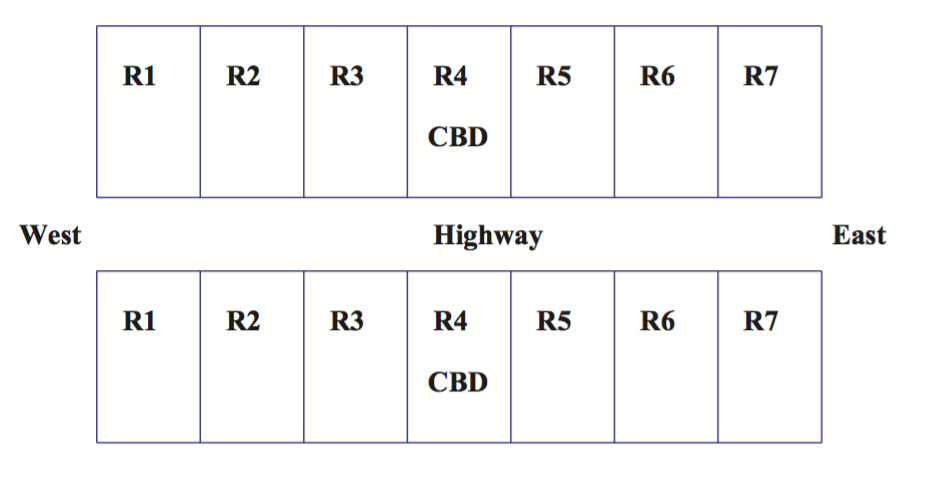
\includegraphics[width = 8cm, height=6cm]{figure/lesage.png}
\end{figure}

We observe the following set of the sample data for these regions that relates travel times to the CBD (in minutes) contained in the dependent variable vector $\vy$ to distance (in miles) and population density (population per square block) of the regions in the two columns of the matrix $\mX$.

\begin{figure}[H]
		    \centering 
		      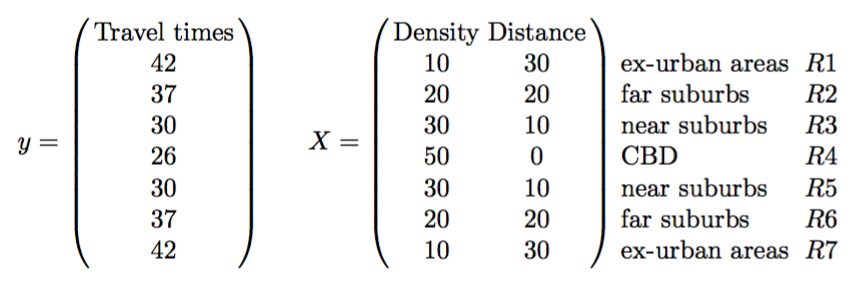
\includegraphics[width = 8cm, height=6cm]{figure/lesage2.png}
\end{figure}	

According to \cite{lesage2010introduction}, the pattern of longer travel times for more distant regions R1 and R7 versus nearer R3 and R5 found in vector $\vy$ seems to clearly violate independence, since travel times appear similar for neighboring regions (see also Example \ref{example:commuting-Kirby}). However one can argue that the observed pattern is not due to spatial dependence, but rather it is explained by the variables Distance and Density associated with each region, since these also appear similar for neighboring regions. Note that even for individual residing in the CBD, it takes time to go somewhere else in the CBD. Therefore, the travel time for intra-CBD travel is 26 minutes despite having a distance of 0 miles. 

If we assume that the observed data was collected in a given day and averaged over a 24-hour period, it can be hypothesized that congestion effects that arise from the shared highway can explain the observed patter of travel times.  It is reasonable to claim that longer travel times in one region should lead to longer travel times in neighboring regions on any given day. This is because commuters pass from one region to another as they travel along the highway to the CBD.

Congestion effects represent one type of spatial spillover, which do not occur simultaneously, but require some time for the traffic delay to arise. From a modeling point of view, this effect cannot be captured by OLS model with distance and density as independent variables. These are dynamic feedback effects from travel time on a particular day that impact travel times of neighboring regions in the short time interval required for the traffic delay to occur. Since the explanatory variable distance would not change from day to day, and population density would change very slowly on a daily time scale, these variables would not be capable of explaining daily delay phenomena. 

A better way of explaining congestion is by the following DGP: 

\begin{equation*}
\vy = \rho_0\mW\vy + \mX\vbeta_0 + \vepsi, 
\end{equation*}
%
such that:
\begin{equation*}
\widehat{\vy} = \left(\mI_n - \widehat{\rho}\mW\right)^{-1}\mX\widehat{\vbeta},
\end{equation*}
%
where the estimated parameters are $\widehat{\vbeta} = (0.135, 0.561)'$ and $\widehat{\rho} = 0.640$ (assume that somehow we have estimated these parameters). Note that the estimated spatial autoregressive parameters indicates positive spatial dependence in the commuting times. 

\subsubsection{Computing Effects in R}

Now think about the following question: What would be the estimated spillovers if region $R2$ doubles its population density? To answer this question we first obtain the predicted values of travel times before the change.\footnote{Note that there is a typo in \cite{lesage2010introduction}, because in their equation (1.19) they double distance, not density.} That is, we first obtain:

\begin{equation*}
\widehat{\vy}^{(1)} = \left(\mI_n - \widehat{\rho}\mW\right)^{-1}\mX\widehat{\vbeta}.
\end{equation*}

\begin{knitrout}
\definecolor{shadecolor}{rgb}{0.969, 0.969, 0.969}\color{fgcolor}\begin{kframe}
\begin{alltt}
\hlcom{# Estimated coefficients}
\hlstd{b} \hlkwb{<-} \hlkwd{c}\hlstd{(}\hlnum{0.135}\hlstd{,} \hlnum{0.561}\hlstd{)}
\hlstd{rho} \hlkwb{<-} \hlnum{0.642}

\hlcom{# W and X}
\hlstd{X} \hlkwb{<-} \hlkwd{cbind}\hlstd{(}\hlkwd{c}\hlstd{(}\hlnum{10}\hlstd{,} \hlnum{20}\hlstd{,} \hlnum{30}\hlstd{,} \hlnum{50}\hlstd{,} \hlnum{30}\hlstd{,} \hlnum{20}\hlstd{,} \hlnum{10}\hlstd{),}
           \hlkwd{c}\hlstd{(}\hlnum{30}\hlstd{,} \hlnum{20}\hlstd{,} \hlnum{10}\hlstd{,} \hlnum{0}\hlstd{,} \hlnum{10}\hlstd{,} \hlnum{20}\hlstd{,} \hlnum{30}\hlstd{))}
\hlstd{W} \hlkwb{<-} \hlkwd{cbind}\hlstd{(}\hlkwd{c}\hlstd{(}\hlnum{0}\hlstd{,} \hlnum{1}\hlstd{,} \hlnum{0}\hlstd{,} \hlnum{0}\hlstd{,} \hlnum{0}\hlstd{,} \hlnum{0}\hlstd{,} \hlnum{0}\hlstd{),}
           \hlkwd{c}\hlstd{(}\hlnum{1}\hlstd{,} \hlnum{0}\hlstd{,} \hlnum{1}\hlstd{,} \hlnum{0}\hlstd{,} \hlnum{0}\hlstd{,} \hlnum{0}\hlstd{,} \hlnum{0}\hlstd{),}
           \hlkwd{c}\hlstd{(}\hlnum{0}\hlstd{,} \hlnum{1}\hlstd{,} \hlnum{0}\hlstd{,} \hlnum{1}\hlstd{,} \hlnum{0}\hlstd{,} \hlnum{0}\hlstd{,} \hlnum{0}\hlstd{),}
           \hlkwd{c}\hlstd{(}\hlnum{0}\hlstd{,} \hlnum{0}\hlstd{,} \hlnum{1}\hlstd{,} \hlnum{0}\hlstd{,} \hlnum{1}\hlstd{,} \hlnum{0}\hlstd{,} \hlnum{0}\hlstd{),}
           \hlkwd{c}\hlstd{(}\hlnum{0}\hlstd{,} \hlnum{0}\hlstd{,} \hlnum{0}\hlstd{,} \hlnum{1}\hlstd{,} \hlnum{0}\hlstd{,} \hlnum{1}\hlstd{,} \hlnum{0}\hlstd{),}
           \hlkwd{c}\hlstd{(}\hlnum{0}\hlstd{,} \hlnum{0}\hlstd{,} \hlnum{0}\hlstd{,} \hlnum{0}\hlstd{,} \hlnum{1}\hlstd{,} \hlnum{0}\hlstd{,} \hlnum{1}\hlstd{),}
           \hlkwd{c}\hlstd{(}\hlnum{0}\hlstd{,} \hlnum{0}\hlstd{,} \hlnum{0}\hlstd{,} \hlnum{0}\hlstd{,} \hlnum{0}\hlstd{,} \hlnum{1}\hlstd{,} \hlnum{0}\hlstd{))}
\hlstd{Ws} \hlkwb{<-} \hlstd{W} \hlopt{/} \hlkwd{rowSums}\hlstd{(W)}

\hlcom{# Prediction}
\hlstd{yhat_1} \hlkwb{<-} \hlkwd{solve}\hlstd{(}\hlkwd{diag}\hlstd{(}\hlkwd{nrow}\hlstd{(W))} \hlopt{-}  \hlstd{rho} \hlopt{*} \hlstd{Ws)} \hlopt \hlkwd{crossprod}\hlstd{(}\hlkwd{t}\hlstd{(X), b)}
\end{alltt}
\end{kframe}
\end{knitrout}

Now we estimate the predicted values of travel times after the change in population density in $R2$ using:

\begin{equation}
\widehat{\vy}^{(2)} = \left(\mI_n - \widehat{\rho}\mW\right)^{-1}\widetilde{\mX}\widehat{\vbeta}
\end{equation}
%
where $\widetilde{\mX}$ is the new matrix reflecting a doubling of the population density of region $R2$.\footnote{For more about prediction in the spatial context see \cite{kelejian2007relative}.} A comparison of predictions $\widehat{\vy}^{(1)}$ and $\widehat{\vy}^{(2)}$ are going to be used to illustrate how the model generates spatial spillovers.  

\begin{knitrout}
\definecolor{shadecolor}{rgb}{0.969, 0.969, 0.969}\color{fgcolor}\begin{kframe}
\begin{alltt}
\hlcom{# Now we double the population density of a single region}
\hlstd{X_d} \hlkwb{<-} \hlkwd{cbind}\hlstd{(}\hlkwd{c}\hlstd{(}\hlnum{10}\hlstd{,} \hlnum{40}\hlstd{,} \hlnum{30}\hlstd{,} \hlnum{50}\hlstd{,} \hlnum{30}\hlstd{,} \hlnum{20}\hlstd{,} \hlnum{10}\hlstd{),}
             \hlkwd{c}\hlstd{(}\hlnum{30}\hlstd{,} \hlnum{20}\hlstd{,} \hlnum{10}\hlstd{,} \hlnum{0}\hlstd{,} \hlnum{10}\hlstd{,} \hlnum{20}\hlstd{,} \hlnum{30}\hlstd{))}

\hlcom{# Compute predicted value after the change}
\hlstd{yhat_2} \hlkwb{<-} \hlkwd{solve}\hlstd{(}\hlkwd{diag}\hlstd{(}\hlkwd{nrow}\hlstd{(W))} \hlopt{-}  \hlstd{rho} \hlopt{*} \hlstd{Ws)} \hlopt \hlkwd{crossprod}\hlstd{(}\hlkwd{t}\hlstd{(X_d), b)}

\hlcom{# Results}
\hlstd{result} \hlkwb{<-} \hlkwd{cbind}\hlstd{(yhat_1, yhat_2, yhat_2} \hlopt{-} \hlstd{yhat_1)}
\hlkwd{colnames}\hlstd{(result)} \hlkwb{<-} \hlkwd{c}\hlstd{(}\hlstr{"y1"}\hlstd{,} \hlstr{"y2"}\hlstd{,} \hlstr{"y2 - y1"}\hlstd{)}
\hlkwd{round}\hlstd{(result,} \hlnum{2}\hlstd{)}
\end{alltt}
\begin{verbatim}
##         y1    y2 y2 - y1
## [1,] 41.90 44.46    2.56
## [2,] 36.95 40.93    3.99
## [3,] 29.84 31.28    1.45
## [4,] 25.90 26.43    0.53
## [5,] 29.84 30.03    0.19
## [6,] 36.95 37.03    0.08
## [7,] 41.90 41.95    0.05
\end{verbatim}
\begin{alltt}
\hlkwd{sum}\hlstd{(yhat_2} \hlopt{-} \hlstd{yhat_1)}
\end{alltt}
\begin{verbatim}
## [1] 8.846915
\end{verbatim}
\end{kframe}
\end{knitrout}

The two set of predictions show that the change in region $R2$ population density has a direct effect that increases the commuting times for residents of region $R2$ by $\approx$4 minutes. It also has an indirect or spillover effect that produces an increase in commuting times for the other six regions. Furthermore, it can be noticed that the increase in commuting times for neighboring regions $R1$ and $R3$ are the greatest and these spillovers decline as we move to regions in the sample that are located farther away from region $R2$ where the change in population density occurred. 

What is the cumulative indirect impacts? Adding up the increased commuting times across all other regions (excluding the own-region change in commuting time), we find that equals $\approx  4.86 (2.56 + 1.45 + 0.53 + 0.19 + 0.08 + 0.05)$ minutes, which is larger than the direct (own-region) impact of 4 minutes. Finally, the total impact of all residents of the seven regions from the change in population density of region $R2$ is the sum of the direct and indirect effects, or 8.85 minutes increase in travel times to the CBD. 

Now assume that the OLS estimates for the example above are: $\widehat{\vbeta}_{OLS} = \left[0.55, 1.25\right]$. Using these estimates we compute the OLS predictions based on the matrices $\mX$ and $\widetilde{\mX}$ as shown above.

\begin{knitrout}
\definecolor{shadecolor}{rgb}{0.969, 0.969, 0.969}\color{fgcolor}\begin{kframe}
\begin{alltt}
\hlcom{# Ols prediction}
\hlstd{b_ols} \hlkwb{<-} \hlkwd{c}\hlstd{(}\hlnum{0.55}\hlstd{,} \hlnum{1.25}\hlstd{)}
\hlstd{yhat_1} \hlkwb{<-} \hlkwd{crossprod}\hlstd{(}\hlkwd{t}\hlstd{(X), b_ols)}
\hlstd{yhat_2} \hlkwb{<-} \hlkwd{crossprod}\hlstd{(}\hlkwd{t}\hlstd{(X_d), b_ols)}
\hlstd{result} \hlkwb{<-} \hlkwd{cbind}\hlstd{(yhat_1, yhat_2, yhat_2} \hlopt{-} \hlstd{yhat_1)}
\hlkwd{colnames}\hlstd{(result)} \hlkwb{<-} \hlkwd{c}\hlstd{(}\hlstr{"y1"}\hlstd{,} \hlstr{"y2"}\hlstd{,} \hlstr{"y2 - y1"}\hlstd{)}
\hlkwd{round}\hlstd{(result,} \hlnum{2}\hlstd{)}
\end{alltt}
\begin{verbatim}
##        y1   y2 y2 - y1
## [1,] 43.0 43.0       0
## [2,] 36.0 47.0      11
## [3,] 29.0 29.0       0
## [4,] 27.5 27.5       0
## [5,] 29.0 29.0       0
## [6,] 36.0 36.0       0
## [7,] 43.0 43.0       0
\end{verbatim}
\end{kframe}
\end{knitrout}

The results show no spatial spillovers. Only the travel time of $R2$ is affected by the change in population density of region $R2$. It can be also observed that OLS prediction is upward bias.  This is the main message here. An OLS model does no allows for spatial spillover impacts and generates biased marginal effects. 

Now we further explore our formulas and definition from previous Section. As we showed in Equation (\ref{eq:direct_impact}), the impact of changes in the $i$th observation of $x_r$ on $y_i$  is $S_r(W)_{ii}$. Given the SLM structure of our example, this is equivalent to 

\begin{equation*}
\frac{\partial \E(\texttt{CT}_i)}{\partial \texttt{density}_i} = \mS_{density}(\mW)_{ii}, \quad \mbox{where $\mS_{\texttt{density}} = (\mI - \rho \mW)^{-1}\mI\beta_{\texttt{density}}$}.
\end{equation*}

We can compute our $\mS_{\texttt{density}}$ in the following way.
 
\begin{knitrout}
\definecolor{shadecolor}{rgb}{0.969, 0.969, 0.969}\color{fgcolor}\begin{kframe}
\begin{alltt}
\hlcom{# Compute S(W) matrix for density}
\hlstd{b_dens} \hlkwb{<-} \hlnum{0.135}
\hlstd{S} \hlkwb{<-} \hlkwd{solve}\hlstd{(}\hlkwd{diag}\hlstd{(}\hlkwd{nrow}\hlstd{(W))} \hlopt{-}  \hlstd{rho} \hlopt{*} \hlstd{Ws)}  \hlopt \hlkwd{diag}\hlstd{(}\hlkwd{nrow}\hlstd{(W))} \hlopt{*} \hlstd{b_dens}
\hlkwd{colnames}\hlstd{(S)} \hlkwb{<-} \hlkwd{rownames}\hlstd{(S)} \hlkwb{<-} \hlkwd{c}\hlstd{(}\hlstr{"R1"}\hlstd{,} \hlstr{"R2"}\hlstd{,} \hlstr{"R3"}\hlstd{,} \hlstr{"R4"}\hlstd{,} \hlstr{"R5"}\hlstd{,} \hlstr{"R6"}\hlstd{,} \hlstr{"R7"}\hlstd{)}
\end{alltt}
\end{kframe}
\end{knitrout}

Then, the direct impact of doubling population density of $R2$ on the expected value of commuting time for $R2$ is given by
   
\begin{equation*}
  \Delta \E(\texttt{CT}_2) = S_{\texttt{density}}(\mW)_{22} \Delta \texttt{density}_{2} = S_{\texttt{density}}(\mW)_{22} \cdot 20
\end{equation*}

In R, this equals :

\begin{knitrout}
\definecolor{shadecolor}{rgb}{0.969, 0.969, 0.969}\color{fgcolor}\begin{kframe}
\begin{alltt}
\hlcom{# Direct impact of R2 on R2}
\hlkwd{round}\hlstd{(S[}\hlnum{2}\hlstd{,}\hlnum{2}\hlstd{]} \hlopt{*} \hlnum{20}\hlstd{,} \hlnum{2}\hlstd{)}
\end{alltt}
\begin{verbatim}
## [1] 3.99
\end{verbatim}
\end{kframe}
\end{knitrout}

Note that this value is the same as that found using the predicted value procedure:  by doubling population density in  $R2$  increases the commuting times for residents of region $R2$ by $\approx$4 minutes. 

Finding the indirect impact on region $R1$ is similar given Equation \ref{eq:indirect_impact}. The indirect impact on region $R1$ is given by:

\begin{equation*}
  \Delta \E(\texttt{CT}_1) = S_{\texttt{density}}(\mW)_{12} \Delta \texttt{density}_{2} = S_{\texttt{density}}(\mW)_{12} \cdot 20
\end{equation*}

That is:

\begin{knitrout}
\definecolor{shadecolor}{rgb}{0.969, 0.969, 0.969}\color{fgcolor}\begin{kframe}
\begin{alltt}
\hlcom{# Indirect impact of R2 on R1}
\hlkwd{round}\hlstd{(S[}\hlnum{1}\hlstd{,}\hlnum{2}\hlstd{]} \hlopt{*} \hlnum{20}\hlstd{,} \hlnum{2}\hlstd{)}
\end{alltt}
\begin{verbatim}
## [1] 2.56
\end{verbatim}
\end{kframe}
\end{knitrout}

Again, note that is the same value computed before: An increase of 100\% of population density in $R2$ implies an increase of travel time of region $R1$ to CBD of about 2.56 minutes, after considering all feedback effects. 


An interesting question would be the following: What would be the impact on commuting time on $R1$ if population density increases by 20 in all the Regions? To answer this question, we should recall our definition \ref{def:ATIT} states that the sum across the $i$th row of $\mS_{r}(\mW)$ would be represent the total impact on individual observation $y_i$ resulting from changing the $r$th explanatory variable by the same amount across $n$ observations. 
   
\begin{knitrout}
\definecolor{shadecolor}{rgb}{0.969, 0.969, 0.969}\color{fgcolor}\begin{kframe}
\begin{alltt}
\hlcom{# ATIT}
\hlkwd{round}\hlstd{(}\hlkwd{sum}\hlstd{(S[}\hlnum{1}\hlstd{, ])} \hlopt{*} \hlnum{20}\hlstd{,} \hlnum{2}\hlstd{)}
\end{alltt}
\begin{verbatim}
## [1] 7.54
\end{verbatim}
\end{kframe}
\end{knitrout}

This number implies that the total impact to R1 will be an increase of commuting time of $\approx 7.5$ minutes. Using the formula for ATIT gives the same result:

\begin{knitrout}
\definecolor{shadecolor}{rgb}{0.969, 0.969, 0.969}\color{fgcolor}\begin{kframe}
\begin{alltt}
\hlcom{# ATIT}
\hlstd{n} \hlkwb{<-} \hlkwd{nrow}\hlstd{(W)}
\hlstd{vones} \hlkwb{<-} \hlkwd{rep}\hlstd{(}\hlnum{1}\hlstd{, n)}
\hlkwd{round}\hlstd{(((}\hlkwd{t}\hlstd{(vones)} \hlopt \hlstd{S} \hlopt \hlstd{vones)} \hlopt{/} \hlstd{n )} \hlopt{*} \hlnum{20}\hlstd{,} \hlnum{2}\hlstd{)}
\end{alltt}
\begin{verbatim}
##      [,1]
## [1,] 7.54
\end{verbatim}
\end{kframe}
\end{knitrout}

Similarly, we could ask: What would be the impact of increasing density by 20 in $R1$ on all the other regions? This is equivalent to our definition \ref{def:ATIF} which state that the sum down the $j$th column of $\mS_r(\mW)$ would yield the total impact over all $y_i$ from changing the $r$th explanatory variable by an amount in the $j$th observation.

\begin{knitrout}
\definecolor{shadecolor}{rgb}{0.969, 0.969, 0.969}\color{fgcolor}\begin{kframe}
\begin{alltt}
\hlcom{# ATIF}
\hlkwd{round}\hlstd{(}\hlkwd{sum}\hlstd{(S[,} \hlnum{1}\hlstd{])} \hlopt{*} \hlnum{20}\hlstd{,} \hlnum{2}\hlstd{)}
\end{alltt}
\begin{verbatim}
## [1] 5.54
\end{verbatim}
\end{kframe}
\end{knitrout}

In words, increasing density by 20 in $R1$ would imply a total effect  in all the regions of about 7.54 minutes.

Imagine that you are a policy maker and you are considering in implementing a policy to reduce population density and hence reduce commuting time in the regions. However, given that resources are scarce, you must select which region to implement this policy. In order to produce a greater effect of policy you could use the estimated spatial model and look for the region that will have the greatest overall impact (considering feedback effects). Basically, this involves calculating the column sum of $\mS_r(\mW)$ for each region in the following way: 

\begin{knitrout}
\definecolor{shadecolor}{rgb}{0.969, 0.969, 0.969}\color{fgcolor}\begin{kframe}
\begin{alltt}
\hlcom{# Computing colsums of S(W)}
\hlkwd{round}\hlstd{(}\hlkwd{colSums}\hlstd{(S),} \hlnum{2}\hlstd{)}
\end{alltt}
\begin{verbatim}
##   R1   R2   R3   R4   R5   R6   R7 
## 0.28 0.44 0.40 0.39 0.40 0.44 0.28
\end{verbatim}
\end{kframe}
\end{knitrout}
   
Note that the impact of decreasing population density by 1 will have a greater reduction in commuting time if applied in regions $R2$ and $R6$ (why?)

Finally, the average direct, indirect and total effects of an increase in 1 in population density in all the regions can be computed as follows. 

\begin{knitrout}
\definecolor{shadecolor}{rgb}{0.969, 0.969, 0.969}\color{fgcolor}\begin{kframe}
\begin{alltt}
\hlcom{# Average Direct Impact }
\hlstd{ADI} \hlkwb{<-} \hlkwd{sum}\hlstd{(}\hlkwd{diag}\hlstd{(S))} \hlopt{/} \hlkwd{nrow}\hlstd{(W)}
\hlkwd{round}\hlstd{(ADI,} \hlnum{4}\hlstd{)}
\end{alltt}
\begin{verbatim}
## [1] 0.1837
\end{verbatim}
\begin{alltt}
\hlcom{# Average Total Impact }
\hlstd{Total} \hlkwb{<-} \hlkwd{crossprod}\hlstd{(}\hlkwd{rep}\hlstd{(}\hlnum{1}\hlstd{,} \hlkwd{nrow}\hlstd{(W)), S)} \hlopt \hlkwd{rep}\hlstd{(}\hlnum{1}\hlstd{,} \hlkwd{nrow}\hlstd{(W))} \hlopt{/} \hlkwd{nrow}\hlstd{(W)}
\hlkwd{round}\hlstd{(Total,} \hlnum{4}\hlstd{)}
\end{alltt}
\begin{verbatim}
##        [,1]
## [1,] 0.3771
\end{verbatim}
\begin{alltt}
\hlcom{# Average Indirect Impact}
\hlkwd{round}\hlstd{(Total} \hlopt{-} \hlstd{ADI,} \hlnum{4}\hlstd{)}
\end{alltt}
\begin{verbatim}
##        [,1]
## [1,] 0.1934
\end{verbatim}
\end{kframe}
\end{knitrout}

Equation (\ref{eq:total_effect_simple}) of Example \ref{example:pollution-kim}, we show that the total effect can be also be computed as $\beta_r / (1 - \rho)$. We know show that this proposition is true for our example

\begin{knitrout}
\definecolor{shadecolor}{rgb}{0.969, 0.969, 0.969}\color{fgcolor}\begin{kframe}
\begin{alltt}
\hlcom{#Check total effect}
\hlstd{b_dens} \hlopt{/} \hlstd{(}\hlnum{1} \hlopt{-} \hlstd{rho )}
\end{alltt}
\begin{verbatim}
## [1] 0.377095
\end{verbatim}
\end{kframe}
\end{knitrout}

\subsubsection{Cumulative Effects}

The main idea of this exercise is to show how the change in some explanatory variable produces changes in the independent variable in all the spatial units by decomposing them into cumulative and marginal impacts for different order of neighbors as explained in Section \ref{sec:partitioning-effects}. 
    
First, we load the package \pkg{expm} which will allow us to compute power of matrices in a loop. Then we create the estimated coefficients along with the $\mW$ matrix:

\begin{knitrout}
\definecolor{shadecolor}{rgb}{0.969, 0.969, 0.969}\color{fgcolor}\begin{kframe}
\begin{alltt}
\hlcom{# Package to compute power of a matrix}
\hlkwd{library}\hlstd{(}\hlstr{"expm"}\hlstd{)}
\end{alltt}
\end{kframe}
\end{knitrout}

In order to create the decomposition for the ADI, AII and ATI, we create the following loop from $q = 0$ to $q = 10$:

\begin{knitrout}
\definecolor{shadecolor}{rgb}{0.969, 0.969, 0.969}\color{fgcolor}\begin{kframe}
\begin{alltt}
\hlcom{## Loop for decomposition}
\hlstd{out} \hlkwb{<-} \hlkwd{matrix}\hlstd{(}\hlnum{NA}\hlstd{,} \hlkwc{nrow} \hlstd{=} \hlnum{11}\hlstd{,} \hlkwc{ncol} \hlstd{=} \hlnum{3}\hlstd{)}             \hlcom{# Matrix for the results }
\hlkwd{colnames}\hlstd{(out)} \hlkwb{<-} \hlkwd{c}\hlstd{(}\hlstr{"Total"}\hlstd{,} \hlstr{"Direct"}\hlstd{,} \hlstr{"Indirect"}\hlstd{)}  \hlcom{# colnames}
\hlkwd{rownames}\hlstd{(out)} \hlkwb{<-} \hlkwd{paste}\hlstd{(}\hlstr{"q"}\hlstd{,} \hlkwc{sep} \hlstd{=} \hlstr{"="}\hlstd{,} \hlkwd{seq}\hlstd{(}\hlnum{0}\hlstd{,} \hlnum{10}\hlstd{))} \hlcom{# rownames}

\hlkwa{for} \hlstd{(q} \hlkwa{in} \hlnum{0}\hlopt{:}\hlnum{10}\hlstd{) \{}
  \hlkwa{if} \hlstd{(q} \hlopt{==} \hlnum{0}\hlstd{) \{}                                    \hlcom{# If q=0, then Sr = I * beta}
    \hlstd{S} \hlkwb{<-} \hlkwd{diag}\hlstd{(n)} \hlopt{*} \hlstd{b_dens}
  \hlstd{\}} \hlkwa{else} \hlstd{\{}
    \hlstd{S} \hlkwb{<-} \hlstd{(rho} \hlopt{^} \hlstd{q} \hlopt{*} \hlstd{Ws} \hlopt \hlstd{q)}  \hlopt{*} \hlstd{b_dens}
  \hlstd{\}}
  \hlstd{q} \hlkwb{<-} \hlstd{q} \hlopt{+} \hlnum{1}                                       \hlcom{# the row = 0 doesn't exist!}
  \hlstd{out[q,} \hlnum{2}\hlstd{]} \hlkwb{<-} \hlkwd{sum}\hlstd{(}\hlkwd{diag}\hlstd{(S))} \hlopt{/} \hlstd{n}
  \hlstd{out[q,} \hlnum{1}\hlstd{]} \hlkwb{<-} \hlkwd{crossprod}\hlstd{(}\hlkwd{rep}\hlstd{(}\hlnum{1}\hlstd{, n), S)} \hlopt \hlkwd{rep}\hlstd{(}\hlnum{1}\hlstd{, n)} \hlopt{/} \hlstd{n}
  \hlstd{out[q,} \hlnum{3}\hlstd{]} \hlkwb{<-} \hlstd{out[q,} \hlnum{1}\hlstd{]} \hlopt{-} \hlstd{out[q,} \hlnum{2}\hlstd{]}
\hlstd{\}}
\end{alltt}
\end{kframe}
\end{knitrout}

The results are the following

\begin{knitrout}
\definecolor{shadecolor}{rgb}{0.969, 0.969, 0.969}\color{fgcolor}\begin{kframe}
\begin{alltt}
\hlcom{# Print results}
\hlkwd{round}\hlstd{(out,} \hlnum{4}\hlstd{)}
\end{alltt}
\begin{verbatim}
##       Total Direct Indirect
## q=0  0.1350 0.1350   0.0000
## q=1  0.0867 0.0000   0.0867
## q=2  0.0556 0.0318   0.0238
## q=3  0.0357 0.0000   0.0357
## q=4  0.0229 0.0106   0.0123
## q=5  0.0147 0.0000   0.0147
## q=6  0.0095 0.0039   0.0056
## q=7  0.0061 0.0000   0.0061
## q=8  0.0039 0.0015   0.0024
## q=9  0.0025 0.0000   0.0025
## q=10 0.0016 0.0006   0.0010
\end{verbatim}
\begin{alltt}
\hlkwd{round}\hlstd{(}\hlkwd{colSums}\hlstd{(out),} \hlnum{4}\hlstd{)}
\end{alltt}
\begin{verbatim}
##    Total   Direct Indirect 
##   0.3742   0.1834   0.1909
\end{verbatim}
\end{kframe}
\end{knitrout}

This table shows both the cumulative and partitioned direct, indirect and total impacts associated with orders 0 to 10 for the SLM. The cumulative direct impact from previous section equal to 0.1837, which given the coefficient 0.1350 indicates that \emph{there is a feedback equal to} (0.1837 - 0.1350) = 0.0487 arising from each region impacting neighbors that in turn impacts neighbors to neighbors and so on.

The column sum of the matrix \texttt{out} shows that by the time we reach 10th-order neighbors we have accounted for 0.1834 of the 0.1837 cumulative direct effect. It is important noting that for $\mW^0$ there is no indirect effect, only direct effects, and for $\mW^1$ there is no direct effect, only indirect. To see this, note that when $q=0$ we obtain $\mW^0 = \mI_n$:

\begin{knitrout}
\definecolor{shadecolor}{rgb}{0.969, 0.969, 0.969}\color{fgcolor}\begin{kframe}
\begin{alltt}
\hlstd{Ws} \hlopt \hlnum{0}
\end{alltt}
\begin{verbatim}
##      [,1] [,2] [,3] [,4] [,5] [,6] [,7]
## [1,]    1    0    0    0    0    0    0
## [2,]    0    1    0    0    0    0    0
## [3,]    0    0    1    0    0    0    0
## [4,]    0    0    0    1    0    0    0
## [5,]    0    0    0    0    1    0    0
## [6,]    0    0    0    0    0    1    0
## [7,]    0    0    0    0    0    0    1
\end{verbatim}
\end{kframe}
\end{knitrout}

Thus,  we have $\mS_r(\mW) = \mI_n\beta_r = 0.1350 \mI_n$. When $q= 1$ we have only indirect effect since there are zero elements on the diagonal of the matrix $\mW$. This also occurs for  $q = 3, 5, 7, 9$: 

\begin{knitrout}
\definecolor{shadecolor}{rgb}{0.969, 0.969, 0.969}\color{fgcolor}\begin{kframe}
\begin{alltt}
\hlstd{Ws} \hlopt \hlnum{1}
\end{alltt}
\begin{verbatim}
##      [,1] [,2] [,3] [,4] [,5] [,6] [,7]
## [1,]  0.0  1.0  0.0  0.0  0.0  0.0  0.0
## [2,]  0.5  0.0  0.5  0.0  0.0  0.0  0.0
## [3,]  0.0  0.5  0.0  0.5  0.0  0.0  0.0
## [4,]  0.0  0.0  0.5  0.0  0.5  0.0  0.0
## [5,]  0.0  0.0  0.0  0.5  0.0  0.5  0.0
## [6,]  0.0  0.0  0.0  0.0  0.5  0.0  0.5
## [7,]  0.0  0.0  0.0  0.0  0.0  1.0  0.0
\end{verbatim}
\begin{alltt}
\hlstd{Ws} \hlopt \hlnum{3}
\end{alltt}
\begin{verbatim}
##       [,1]  [,2]  [,3]  [,4]  [,5]  [,6]  [,7]
## [1,] 0.000 0.750 0.000 0.250 0.000 0.000 0.000
## [2,] 0.375 0.000 0.500 0.000 0.125 0.000 0.000
## [3,] 0.000 0.500 0.000 0.375 0.000 0.125 0.000
## [4,] 0.125 0.000 0.375 0.000 0.375 0.000 0.125
## [5,] 0.000 0.125 0.000 0.375 0.000 0.500 0.000
## [6,] 0.000 0.000 0.125 0.000 0.500 0.000 0.375
## [7,] 0.000 0.000 0.000 0.250 0.000 0.750 0.000
\end{verbatim}
\end{kframe}
\end{knitrout}


Also, the row-stochastic nature of $\mW$ leads to an average of the sum of the rows that takes the form $\beta_r \times \rho= 0.135\times 0.642 = 0.0867$, when $q=1$.

The matrix \texttt{out} also shows that both direct and indirect effects fall out as the order of neighbors increases, however the indirect or spatial spillovers effects decay more slowly as we move to higher-order neighbors. 


%**********************************************
%\section{Criticisms of Spatial Econometrics}
%**********************************************

% The concepts of causality and endogeneity have not been elaborated so much in a spatial context.\\
% 
% The goal of spatial dependence is to measure the effects of proximity. Other studies try to isolate the effect of proximity.\\
% 
% Another problem using spatial data analysis is that important variables are highly correlated and no study includes all relevant variables (Problem of correlated missing variables \citep{mcmillen2010issues}).\\
% 
% In some cases when the units of observation can be located in some geographical space it is possible that location is irrelevant for understanding data pertaining to those units. In this case, we might say that the spatial dimension is random. In other cases, including the spatial dimension to the problem is important.\\
% 
% 
% There are three papers that critique spatial econometrics.
% 
% \begin{enumerate}
% 	\item \cite{gibbons2012mostly} state that identification is almost always impossible with standard spatial econometric practice.
% 	\item \cite{mcmillen2012perspectives} posits that spatial econometrics rests on very restrictive assumptions and that identification is difficult. Nonparametric approaches are better.
% 	\item \cite{corrado2012economics} state that standard spatial econometric has too often been misapplied. Namely, there is not enough emphasis on both theory or in simply forming a conceptual framework to understand spatial spillovers.
% \end{enumerate}	
% 
% 
% According to 

\section{Exercises}

\begin{exercises}

    \exercise Assume three regions with row-normalized spatial weight matrix given in Equation \eqref{eq:w_mat_ex_spill}. Derive the total, direct an indirect effects for the following models:
        \begin{enumerate}
            \item Spatial Durbin Model given by:
		\begin{equation}
			\vy = \rho \mW \vy + \alpha \vones_n + \mX \vbeta + \mW \mX \vtheta + \vepsi
		\end{equation}
            \item Spatial Lag Model given by:
		\begin{equation}
			\vy = \rho \mW \vy + \alpha \vones_n + \mX\vbeta + \vepsi
		\end{equation}
		   \item Spatial Durbin Error Model given by:
		\begin{eqnarray}
			\vy &=& \alpha \vones_n + \mX\vbeta + \mW\mX\vtheta + \vu \\
			\vu &=& \lambda \mW\vu + \vepsi
		\end{eqnarray}
		\item OLS given by:
		\begin{equation}
			\vy = \alpha \vones_n + \mX\vbeta + \vepsi
		\end{equation}
		\item Spatial Error model given by:
		
		\begin{equation}
			\begin{aligned}
				\vy &= \alpha \vones_n + \mX\vbeta + \vu \\
				\vu &= \lambda \mW\vu + \vepsi
			\end{aligned}
		\end{equation} 
        \end{enumerate}

    \exercise Consider your results for the SLM and SDM models from Exercise  \ref{lab:2.1}. Show that for the SLM model the ratio between the indirect and the direct effect of a particular explanatory variable is independent of $\beta_k$. Show that this is not the case for the SDM model. What do you conclude?
    
    \exercise  Recall that if the row-sums of $\mW$ is less than or equal to one and $\rho$ is in the proper parameter space, i.e., $\rho <1$, the total average effect for variable $r$ can be computed as $\beta_r / (1 - \rho)$. What is the sign of the parameter that matters the most when calculating the sign of the total effect? Does the $\rho$ or $\beta_r$?

\end{exercises}

%************************************
\part{Estimation Methods}
%*************************************


\chapter{Review of Asymptotic Theory}

This chapter provides some basic definitions and concepts for asymptotic theory. 

%***************************************************
\section{Convergence of Deterministic Sequences}\label{sec:nonstochastic_con}\index{Convergence!deterministic sequences}
%***************************************************

In order to understand the asymptotic behavior of stochastic sequences we need first to refresh some concepts about deterministic (non-random) sequences. Recall that a sequence of nonstochastic real numbers $\left\lbrace a_n\right\rbrace$ converges to $a$ if for any $\epsilon > 0$, there exists $n^* = n^*(\epsilon)$ such that for all $n > n^*$,

\begin{equation*}
	\left| a_n - a\right|<\epsilon, 
\end{equation*}
%
e.g., if $a_n = 2 + 3/n$, then the limit is 2 since $\left| a_n - a\right| =\left| 2 + 3/n - 2\right| = \left|3/n\right|< \epsilon$ for all $n > n^* = 3/\epsilon$. 


\begin{figure}[ht]
  \caption{Convergence of sequence $2 + 3/n$}
    \label{fig:SeqConv}
    \centering
    \begin{minipage}{.9\linewidth}
\begin{knitrout}
\definecolor{shadecolor}{rgb}{0.969, 0.969, 0.969}\color{fgcolor}

{\centering 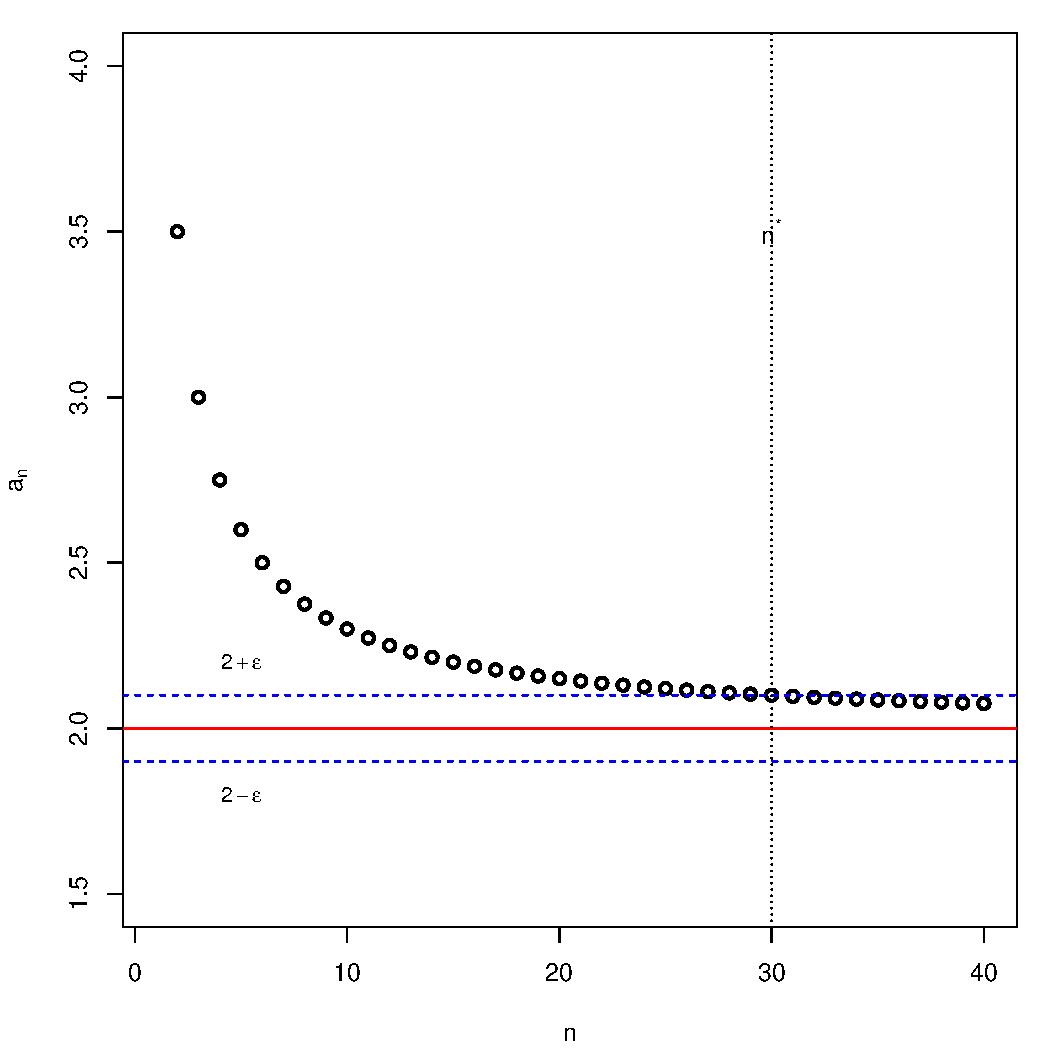
\includegraphics[width=10cm,height=10cm]{figure/SeqConv-1} 

}


\end{knitrout}
\footnotesize
		\emph{Notes: This graphs shows the convergence of the sequence $2 + 3/n$ where $\epsilon = 0.1$ and $a = 2$.}
	\end{minipage}
\end{figure}


Definition \ref{definition:convergence_deterministic} give us a formal statement regarding nonstochastic sequence of numbers.

\begin{definition}[Deterministic convergence]\label{definition:convergence_deterministic}
	The sequence $\left\lbrace b_n: n = 1,2,... \right\rbrace$ of real numbers  converges to the limit $b$ if for every $\epsilon > 0$ there exists and $n^*(\epsilon)$ such that if $n>n^*(\epsilon)$ then $|b_n - b|<\epsilon$. This is also indicated as follows:
\begin{equation*}
\lim_{n\to \infty} b_n = b
\end{equation*}	
\end{definition}

In Definition \ref{definition:convergence_deterministic} by choosing a very small $\epsilon$, we ensure that $b_n$ gets arbitrarily close to its limit $b$ for all $n$ that is sufficiently large. If fact, the smaller $\epsilon$ is, the larger $n(\epsilon)$ will be. So, $\epsilon$ can be interpreted as a prespecified tolerance level for the discrepancy between $b_n$ and $b$. When a limit exists, we say that the sequence $\left\lbrace b_n \right\rbrace$ \textbf{converges} to $b$ as $n$ tends to infinity, written $b_n\to b$ as $n\to \infty$.

Figure~\ref{fig:SeqConv} shows that the sequence $2 + 3/n$ converges to 2. Note that if $\epsilon = 0.1$ then it is always true that $a_n$ will be always between $2 + \epsilon$ and $2 - \epsilon$ if and only if $n \geq n^*= 30$.

In econometric, we talk a lot about sequences of matrices. Probably you are asking yourself, what is a sequence of matrices? Hopefully, the following example will give you some intuition. 

\begin{example}[A sequence of Matrices]\label{example:sequence_matrix}
Let $\mX_n$ be an $n\times 2$ matrix whose $i$th row is defined by the $1\times 2$ vector $\left[1, i\right]$ so that

\begin{equation*}
\mX_n = \begin{pmatrix}
  1 & 1 \\
  1 & 2 \\
  \vdots & \vdots\\
  1 & n
\end{pmatrix}
\end{equation*}

Then

\begin{equation*}
\left\lbrace \begin{pmatrix}
1 & 1\\
1 & 1
\end{pmatrix},
\begin{pmatrix}
  1 & 3/2 \\
  3/2 & 5/2
\end{pmatrix},
\begin{pmatrix}
1 & 2 \\
2 & 14/3
\end{pmatrix}, ...
\right\rbrace
\end{equation*}
%
is a sequence of matrices $\mY_1, \mY_2, \mY_3,...$ defined by the function $\mY_n = \frac{1}{n}\mX_n^\top\mX_n$, where the $n$th element of the sequence is defined as

\begin{equation*}
\mY_n = \begin{pmatrix}
1 & \frac{\sum_{i = 1}^n i}{n} \\
\frac{\sum_{i = 1}^n i}{n} & \frac{\sum_{i = 1}^n i^2}{n}
\end{pmatrix} = 
\begin{pmatrix}
1 & \frac{(n + 1)}{2} \\
\frac{(n + 1)}{2}& \frac{(n +1)(2n +1)}{6}
\end{pmatrix}
\end{equation*}
\end{example}

Now, we formally state the concept of convergence for matrices. 

\begin{definition}[Limit of a Real-Valued Matrix Sequence]
Let $\left\lbrace\mX_n \right\rbrace$ be a sequence whose elements are $q\times k$ real-valued matrices. Suppose there exists a $q\times k$ matrix of real numbers $\mX$ such that $\mX_n\left[i, j\right]\to \mX\left[i, j\right]$ for $i = 1,...,q$ and $j = 1,...,k$. Then the matrix $\mX$ is the limit of the matrix sequence $\left\lbrace\mX_n \right\rbrace$ as $n\to \infty$. If the limit does not exists, the sequence is said to be divergent
\end{definition}

The definition of the limit implies that for a sufficiently large choice of $n$, the matrix $\mX_n$ becomes arbitrarily close to the matrix $\mX$, \textbf{element by element}.


Sometimes, some sequences does not have a limit, but we can say whether they are \textbf{bounded}: 

\begin{definition}[Bounded sequence]\label{definition:bounded_sequence}\index{Convergence!bounded sequences}
 A  sequence $\left\lbrace b_n: n = 1,2,... \right\rbrace$ is \emph{bounded} if and only if there is some $a < \infty$ such that $\left|b_n\right|\leq a$ for all $n = 1,2,...$ Otherwise, we say that $\left\lbrace b_n \right\rbrace$ is \emph{unbounded}.
\end{definition}

Thus, for a sequence of real numbers to be bounded, there must exist a positive number that is larger than the absolute value of each and every number in the sequence. For a sequence that has no limit and is also unbounded, we write $b_n \to \infty$, denoting that the sequence diverges to infinity. 


\begin{example}[Bounded Sequences]
Consider $a_n = (-1)^n$, then $a_n$ does not have a limit, but it is bounded since $-1 \leq a_n \leq 1$. The sequence $a_n = 1/n$ is bounded, since $0 \leq a_n\leq 1$ for all $n = 1,2,...$
\end{example}


\begin{example}[Boundedness and Limit of Matrices]
Consider the following examples:
\begin{enumerate}
 \item Recall the sequence of matrices in Example \ref{example:sequence_matrix}. In this case, only the sequence $\left\lbrace \mY_n\left[1, 1\right]\right\rbrace$ is bounded. All other sequences of matrix elements are unbounded and, in fact, diverge to infinity. Since all the sequences of matrix elements must be bounded for the matrix sequence to converge, the matrix does not have a limit.
 \item Let $\left\lbrace \mX_n\right\rbrace$ be a sequence of matrices such that
 
\begin{equation*}
\mX_n = \begin{pmatrix}
  3n^{-1} & n^{-1} \\
  3       & 1 + n^{-1}
\end{pmatrix}.
\end{equation*}

All four sequences of the matrix elements are bounded, since $\left|3n^{-1}\right|\leq 3$, $\left|n^{-1}\right|\leq 1$, $\left|3\right|\leq 3$, and $\left|1 + n^{-1}\right|\leq 2$, for all $n$. Furthermore, limits exists for all four sequences of matrix elements, since $3n^{-1}\to 0, n^{-1}\to 0, 3\to 3$, and $1 + n^{-1}\to 1$. Thus 

\begin{equation*}
\mX_n\to \mX= \begin{pmatrix}
0 & 0 \\
3 & 1
\end{pmatrix}
\end{equation*}
 \end{enumerate}
\end{example}

Often it is useful to have a measure of the \emph{order of magnitude} of a particular sequence without particularly worrying about its convergence. 
\begin{definition}[Big and little O]\label{definition:big_little_oh}\index{big O}
Consider the following definitions:
	\begin{enumerate}
		\item A sequence $\left\lbrace x_n \right\rbrace $ is $O(n^{\lambda})$ (at most of order $n^{\lambda}$) if $n^{-\lambda}x_n$ is bounded. When $\lambda=0$, $\left\lbrace x_n \right\rbrace $ is bounded, an we also write $x_n=O(1)$.
		\item $\left\lbrace x_n \right\rbrace $ is $o(n^{\lambda})$ if $n^{-\lambda}x_n\to 0$. When $\lambda=0$, $x_n$ converges to zero, and we also write $a_n=o(1)$.
		\item If $\left\lbrace X_n\left[i,j\right]\right\rbrace$ is $O(n^\lambda)$ or $o(n^\lambda)$ for all $i$ and $j$, then the matrix sequence $\left\lbrace \mX_n\right\rbrace$ is said to be $O(n^\lambda)$ or $o(n^\lambda)$
	\end{enumerate}
\end{definition}

The big $O$ notation describes the asymptotic behavior of functions. Basically, it tells you how fast a function grows or declines. 

\begin{remark}
From the definitions we can say that if $X_n = o(n^\lambda)$, then $X_n = O(n^\lambda)$. In other words, \textbf{any convergent sequence is bounded}. The opposite is not true. Recall the example $a_n = (-1)^n$.
\end{remark}

\begin{example}[Order of Magnitude of a Sequence]
Consider the following examples:

\begin{enumerate}
  \item Let $\left\lbrace x_n\right\rbrace$ be defined by $x_n = 3n^3 - n^2 + 2$. Then $\left\lbrace x_n\right\rbrace$ is $O(n^3)$, since $n^{-3}x_n = 3 - n^{-1} + 2n^{-3}$ is bounded. Also $\left\lbrace x_n\right\rbrace$ is $o(n^{3 + \epsilon})$ for any $\epsilon > 0$ since $n^{ - 3 - \epsilon}x_n = 3n^{-\epsilon} - n^{-1 - \epsilon} + 2n^{-3 - \epsilon}\to 0$. For example, Figure \ref{fig:SeqConvBond} plots $n^{-3}x_n$, which is bounded between 4 ($n = 1$) and 2.75 $(n = 2)$. Note also that if we choose $\epsilon = 0.1$, then $n^{3.1}x_n$ clearly converges to 0.
  \item Let $\left\lbrace x_n\right\rbrace$ by defined by $x_n = 3 + n^{-1}$. Then $\left\lbrace x_n\right\rbrace$ is $O(1)$, since $x_n$ is bounded, and $\left\lbrace x_n\right\rbrace$ is $o(n^\epsilon);\forall \epsilon > 0$, since $n^{-3}x_n = 3n^{-\epsilon} + n^{-1 - \epsilon}\to 0$. 
  \item Let the vector sequence $\left\lbrace \vx_n\right\rbrace$ by defined by
  
  \begin{equation*}
    \begin{pmatrix}
    \vx_n\left[1\right] \\
    \vx_n\left[2\right]
    \end{pmatrix}= 
    \begin{pmatrix}
      3n^{-1} \\
      n^{-1}
    \end{pmatrix}.
  \end{equation*}
  Then the vector sequence $\left\lbrace \vx_n\right\rbrace$ is $o(1)$ and $O(1)$, since
  
  \begin{equation*}
    \vx_n \to \begin{pmatrix} 0 \\ 0 \end{pmatrix}
  \end{equation*}
\end{enumerate}
\end{example}

\begin{figure}[ht]
  \caption{Bounded sequence}
    \label{fig:SeqConvBond}
    \centering
    \begin{minipage}{.9\linewidth}
\begin{knitrout}
\definecolor{shadecolor}{rgb}{0.969, 0.969, 0.969}\color{fgcolor}

{\centering 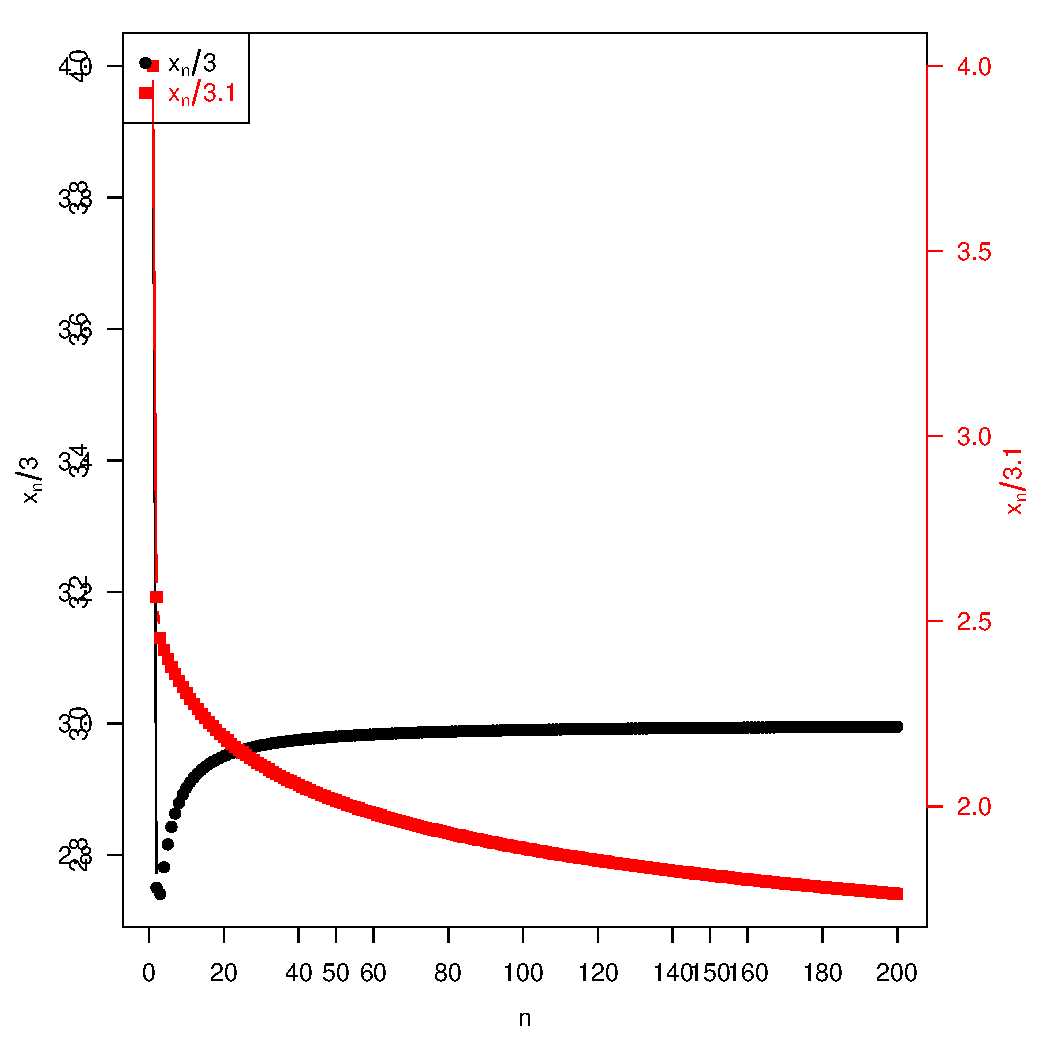
\includegraphics[width=10cm,height=10cm]{figure/SeqConvBoun-1} 

}


\end{knitrout}
\footnotesize
		\emph{Notes: This graphs shows that the sequence $\left\lbrace x_n\right\rbrace$ defined by $x_n = 3n^3 - n^2 + 2$ is $O(n^3)$ and $o(n^{3 + \epsilon})$. For plotting $\epsilon = 0.1$ was selected.}
	\end{minipage}
\end{figure}


%*****************************************
\section{Convergence in Probability}
%****************************************** 

In the previous section we reviewed how a sequence of real number converges to a real number.  What about the sequence of random variables such as econometric estimators? When considering a sequence of \emph{random variables} we cannot be certain that $\left| a_n - a\right|<\epsilon$, even for large $n$, due to the \textbf{randomness}. Instead, we require that \textbf{the probability of being within $\epsilon$ is arbitrarily close to one} as $n\to \infty$. The next definition is more appropriate for convergence in random variables. 

\begin{definition}[Convergence in Probability]\label{definition:convergence_in_probability}\index{convergence in probability}
	A sequence of random variables $\left\{X_n\right\}$ \textbf{convergence in probability} to a constant (non-random) $\alpha$ if, for any $\epsilon>0$,
	
	\begin{equation*}
	\lim_{n\to \infty} \Pr(\left|X_n-\alpha\right|>\epsilon)=0
	\end{equation*}
	
	The constant $\alpha$ is called the \textbf{probability limit} of $X_n$ and is written as $\plim X_n=\alpha$ or $X_n\pto \alpha$. Evidently,
	
	\begin{equation*}
	X_n\pto \alpha\qquad\mbox{is the same as}\qquad X_n-\alpha\pto 0
	\end{equation*}	
\end{definition}

Thus, roughly, convergence in probability states that for large $n$, the probability is high that $X_n$ will be close $\alpha$.

This definition can be understood if we look at Figure \ref{fig:convinprob}. Note that the expression $\left|X_n-\alpha\right|>\epsilon$ can be true or false. The probability that it is true is given by the distribution $F_n(\cdot)$ of $X_n$. Figure \ref{fig:convinprob} shows that the probability that $\left|X_n-\alpha\right|>\epsilon$,  denoted by the red-dashed area outside the interval $\alpha \pm \epsilon$, becomes smaller as $n$ increases. Conversely, the probability of $\left|X_n-\alpha\right|<\epsilon$, given by the blue-dashed area, will become higher and higher as $n\to \infty$. In the limit, this probability should be equal to 1. That is:

\begin{equation*}
	\lim_{n\to \infty} \Pr(\left|X_n-\alpha\right|<\epsilon)=1
\end{equation*}

\begin{figure}[ht]
  \caption{Illustration of convergnce in probability to a constant}
    \label{fig:convinprob}
    \centering
    \begin{minipage}{.9\linewidth}
\begin{knitrout}
\definecolor{shadecolor}{rgb}{0.969, 0.969, 0.969}\color{fgcolor}

{\centering 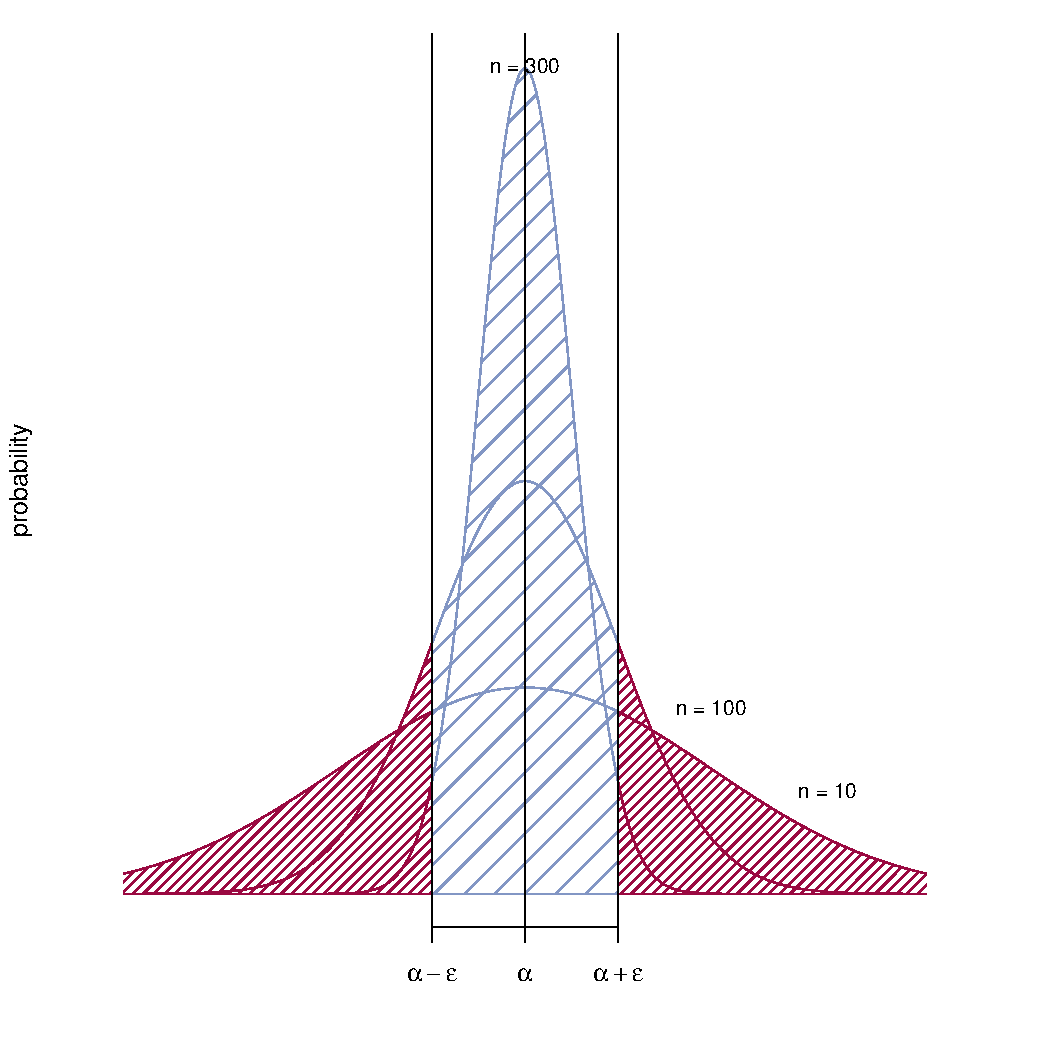
\includegraphics[width=10cm,height=10cm]{figure/convinprob-1} 

}


\end{knitrout}
\footnotesize
		\emph{Notes: This graphs shows that the probability of $\left|X_n-\alpha\right|>\epsilon$, which is denoted by the red-dashed areas, becomes smaller as $n$ increases. }
	\end{minipage}
\end{figure}

Definition (\ref{definition:convergence_in_probability}) can be easily extended to a sequence of random vectors or random matrices (by viewing a matrix as a vector whose elements have been rearranged) by requiring element-by-element convergence in probability. That is, a sequence of $k$-dimensional random vectors $\left\{\vx_n\right\}$ convergences in probability to a $k$-dimensional vector of constants $\valpha$ if, for any $\epsilon>0$,

\begin{equation*}
\lim_{n\to \infty} \Pr(\left\lVert\vx_{n}-\valpha\right\rVert>\epsilon)
\end{equation*}

Note that $\left\| \vx_n - \valpha\right\| $ is the Euclidean distance 

\begin{equation*}
\left[\left(\vx_n - \valpha\right)'\left(\vx_n - \valpha\right)\right]^{1/2} = \sqrt{(x_{1n}-\alpha_1)^2 + ... + (x_{Kn} - \alpha_K)^2} = \left\| \vx_n - \valpha\right\| 
\end{equation*}


Therefore, 

\begin{equation*}
\vx_n \pto \valpha\quad \mbox{iff}\quad \Pr\left[\sqrt{\sum_{j = 1}^k\left(x_{j,n}- x_j\right)^2}> \epsilon\right]\pto 0
\end{equation*}
%
as $n\to \infty$ for $\epsilon >0$ and $\forall j = 1,...,k$, where:

\begin{equation*}
\vx_n = \begin{pmatrix}
          x_{1n} \\
          \vdots \\
          x_{kn}
        \end{pmatrix}
        \quad
        \mbox{and}
        \quad
\valpha = \begin{pmatrix}
            \alpha_1 \\
            \vdots \\
            \alpha_{k}
          \end{pmatrix}
\end{equation*}

\begin{remark}
  $\vx_n \pto \valpha$ if and only if $x_{jn}\pto \alpha_j$ for $j =1, ...,k$. That is, vector convergence in probability is equivalent to component convergence in probability for each component. See our previous discussion of vector sequence.
\end{remark}

\begin{definition}[Probability Limits of Matrices (and Vectors for $k = 1$)]
Let $\left\lbrace \mY_n \right\rbrace$ be a sequence of $m\times k$ random matrices. Then

\begin{equation*}
  \plim \begin{pmatrix}
          Y_n\left[1, 1\right] & \hdots & Y_n\left[1, k\right] \\
          \vdots & \ddots & \vdots \\
          Y_n\left[m, 1\right] & \hdots & Y_n\left[m, k\right]
        \end{pmatrix} = \begin{pmatrix}
          \plim Y_n\left[1, 1\right] & \hdots & \plim Y_n\left[1, k\right] \\
          \vdots & \ddots & \vdots \\
          \plim Y_n\left[m, 1\right] & \hdots & \plim Y_n\left[m, k\right]
        \end{pmatrix}
\end{equation*}
\end{definition}

The expectation $\E(\cdot)$ is a linear operator, that is, \textbf{we cannot} state that $\E\left[\exp(\widehat{\theta})\right] = \exp\left[\E\left(\widehat{\theta}\right)\right]$. Thus, we would like to know if the $\plim$ has the same property. Fortunately, the continuous mapping theorem tell us that we can interchange them. 

\begin{theorem}[Continuous Mapping Theorem]\label{teo:continuous_prob}
	Given a continuous function $g(X)$, if $X_n\pto X$ then $g(X_n)\pto g(X)$ as $n\to \infty$, or equivalently, $\plim \left[g(X_n)\right] = g\left[\plim (X_n)\right]$.
\end{theorem}

The Continuous Mapping Theorem is a very useful theorem. Unlike the expectation operator, it shows that the $\plim$ operator passes through nonlinear functions, provided they are continuous. The lack of this property for the $\E$ operator makes finite sample analysis difficult for many estimators. 


It is useful to know the vector form of this Theorem. Let $\vg:\SR^K\to\SR^J$ be a function continuous at some point $\valpha \in \SR^K$. Then, 

\begin{equation*}
  \vx_n \pto \valpha \implies \vg(\vx_n)\pto \vg(\valpha),
\end{equation*}
%
if $\vg(\cdot)$ is continuous at $\plim \vx_n$.


Now that we have presented the meaning of convergence in probability, it is time to define what we understand for ``consistency'' in econometrics.

\begin{definition}[Consistent Estimator]\label{def:consistent_est}\index{consistent estimator}
  An estimator $\widehat{\vtheta}_n$ of a parameter $\vtheta$ is a consistent estimator $\vtheta$ if and only if
  
  \begin{equation*}
    \plim \widehat{\vtheta}_n = \vtheta,
  \end{equation*}
%
which can also be written as:

  \begin{equation*}
    \widehat{\vtheta}_n \pto \vtheta.
  \end{equation*}
  
\end{definition}

In words, a \textbf{consistent estimator} is an estimator---a rule for computing estimates of a parameter $\vtheta$---having the property that as the number of data used increases without bound, the resulting sequence of estimates converges in probability to $\vtheta$. This means that the distributions of the estimates become more and more concentrated near the true value of the parameters being estimated, so that the probability of the estimator being arbitrary close to $\vtheta$ converges to one. 

\begin{remark}
Convergence in probability is also referred to as weak consistency, and since this has been the most familiar stochastic convergence concept in econometric, the word ``weak'' if often simply dropped.
\end{remark}



\begin{definition}[Strong Convergence in Probability]
	A sequence of random variables $\left\{X_n\right\}$ \textbf{convergence in probability strongly, or, almost surely} to a constant (non-random) $\alpha$ if, for any $\epsilon>0$,
	
	\begin{equation*}
	 \Pr\left(\lim_{n\to \infty}X_n = \alpha\right)=1
	\end{equation*}
	
	This is written $X_n\asto \alpha$, as $n\to \infty$. An equivalent condition for almost sure convergence is
	
	\begin{equation*}
	  \lim_{n\to \infty}\Pr\left(\left|X_m \to X\right| < \epsilon, \forall m\geq n\right) = 1
	\end{equation*}
\end{definition}

The extension to random vector is analogous to that for convergence in probability. Note also that this concept is stronger than convergence in probability; that is, if a sequence converges almost surely, the it converges in probability. 

\begin{remark}
  $\asto \implies \pto$
\end{remark}


In the previous definitions of convergence, the limit is a constant (i.e., a real number). The limit can be a random variable. We say that a sequence of $K$-dimensional random variables $\left \lbrace \vx_n\right\rbrace$ converges to a $k$-dimensional random variable $\vx$ and write $\vx_n\pto \vx$ if $\left\lbrace \vx_n - \vx\right\rbrace$ converges to $\vzeros$. The same applies for almost sure convergence.


We will make frequent use of a special case of convergence in probability, \textbf{convergence in mean square} or \textbf{convergence in quadratic mean}

\begin{theorem}[Convergence in Quadratic Mean]\label{teo:conv_qm}
If $X_n$ has mean $\mu_n$ and variance $\sigma^2_n$ such that the ordinary limits of $\mu_n$ and $\sigma^2_n$ are $c$ and 0, respectively, then $X_n$ converges in mean square to c,

\begin{equation*}
  X_n\qmto c
\end{equation*}
%
and 

\begin{equation*}
  \plim X_n = c.
\end{equation*}
\end{theorem}

This theorem implies that $X_n\qmto c \implies X_n\pto c$. The conditions for convergence in mean square are usually easier to verify than those for the more general form.

The vector form of this type of convergence is the following. We say that the sequence of random vectors $\vx_1, \vx_2,...,\vx_n$ converges in quadratic mean to the random vector $\vz$ if $\E(\vx_n\vx_n')$ and $\E(\vx\vx')$ exists for all $n$ if

\begin{equation*}
  \lim_{n\to \infty} \E\left[\left(\vx_n  - \vx\right)'\left(\vx_n  - \vx\right)\right] = \vzeros
\end{equation*}

A special case of convergence in quadratic mean occurs when $\vx$, instead of being a random vector, is a vector of unknown parameters, say $\vtheta$, and $\vx_n$ is an estimator for $\vtheta$. Under these circumstances we can write:

\begin{equation}\label{eq:biase_var}
  \begin{aligned}
    \E\left[\left(\vx_n  - \vx\right)'\left(\vx_n  - \vx\right)\right] & = \left(\E\left[\vx_n\right]  - \vtheta\right)'\left(\E\left[\vx_n\right]  - \vtheta\right) + \E\left[\left(\vx_n - \E\left[\vx_n\right]\right)'\left(\vx_n - \E\left[\vx_n\right]\right)\right] \\
    & = \sum_{k = 1}^K\mbox{bias}^2(x_{kn}) + \sum_{k = 1}^K \var(x_{kn})
  \end{aligned}
\end{equation}
%
where $x_{kn}$ is the $k$th element of $\vx_n$ that is assumed to be $K$ dimensional. Thus from (\ref{eq:biase_var}) $\vx_n$ converges to $\vzeros$ in quadratic mean if and only if the bias and variance of $\vx_n$ approach zero as $n\to\infty$. This result, and the fact that Chebyshev's inequality can be used to prove that convergence in quadratic mean implies convergence in probability. See below.

Another definitions that will be useful to show other ways of convergences are the Chebyshev's inequality and Markov's inequality.

\begin{definition}[Chebyshev's inequality]\label{definition:chebyshev_ineq}
	 If $X_n$ is a random variable with mean $\mu$ and \textbf{finite variance}, then, for every $\delta > 0$,
	 
	 \begin{equation*}
	 \Pr\left[\left| X_n - \mu\right|\geq \delta \right]\leq \frac{\E\left[(X_n - \mu)^2\right]}{\delta ^2}
	 \end{equation*}
\end{definition}

To prove the Chebyshev inequality, we use the Markov's Inequality

\begin{definition}[Markov's inequality]\label{definition:chebyshev_ineq}
	 If $X_n$ is a nonnegative random variable, then for every $\delta > 0$,
	 
	 \begin{equation*}
	 \Pr\left[X_n \geq \delta \right]\leq \frac{\E\left[X_n\right]}{\delta}
	 \end{equation*}
\end{definition}


An useful theorem is the following:

\begin{theorem}[Consistency of the sample mean]\label{teo:consistency_sample_mean}
The mean of a random sample from any population with finite mean $\mu$ and finite variance $\sigma^2$ is a consistent estimator of $\mu$.
\end{theorem}

\begin{proof}[Proof of consistency of the sample mean]
Since $\E(\overline{X}_n) = \mu$ and $\var(\overline{X}_n) = \sigma^2/n$. Therefore, using Theorem \ref{teo:conv_qm} (Convergence in quadratic mean)

\begin{equation*}
\overline{X}_n \qmto \mu \implies \overline{X}_n \pto \mu
\end{equation*}
\end{proof}

\begin{theorem}[Sufficient Conditions for Consistency]\label{teo:chebyshev}
Chebyshev's inequality implies that a sufficient conditions for an estimator based on a sample of size $n$, say $\widehat{\theta}_n$, say to be consistent for $\theta$ are:

\begin{equation*}
  \begin{aligned}
    \E\left(\widehat{\theta}_n\right) & = \theta_0 \\
    \lim_{n \to \infty} \var\left(\widehat{\theta}_n\right)& = 0
  \end{aligned}
\end{equation*}

If these two requirements are met, then:

\begin{equation*}
\widehat{\vtheta}_n\pto \vtheta
\end{equation*}
\end{theorem}

\begin{proof}[Proof of consistency of unbiased estimator]
  Since $\widehat{\theta}_n$ is unbiased, using Chebyshev's inequality \ref{definition:chebyshev_ineq} we obtain:
  
  \begin{equation*}
    \Pr\left[\left| \widehat{\theta}_n - \theta\right|\geq \delta \right]\leq \frac{\var(\widehat{\theta}_n)}{\delta ^2}
  \end{equation*}
  
  If $\lim_{n\to\infty}\var(\widehat{\theta}(X_1,...,X_n)) = 0$, then $\Pr\left[\left| \widehat{\theta}_n - \theta\right|\geq \delta \right]\to 0$, so $\widehat{\theta}_n\pto \theta$
\end{proof}

\begin{example}
For the normal case, we have that $\E(s^2) = \sigma^2$ and $\var(s^2) = 2\sigma^4 / (n - 1)\to 0$ as $n\to \infty$, hence $s^2\pto \sigma^2$
\end{example}


\begin{example}
For the Bernoulli case, we know that $\E(\overline{X}) = \theta$ and $\var(\overline{X}) = \theta (1- \theta)/ n \to 0$ as $n\to \infty$, hence $\overline{X}\pto \theta$
\end{example}

Therefore, another alternative method for proving that some estimator $\widehat{\vtheta}$ is consistent is to demonstrate that its unbiased and its covariance matrix approaches zero as $n\to\infty$.

\begin{remark}
Theorem \ref{teo:chebyshev} (Consistency of Unbiased Estimator) is only a sufficient condition for consistency. Failing to satisfy this condition does not necessarily imply that the estimator is inconsistent. 
\end{remark}

%It is worth emphasizing that although convergence in quadratic mean implies convergence in probability, the converse is not true. Therefore if $\lim (\E(\vx_n) - \vtheta) = \vzeros$ and $\lim \E\left[\left(\vx_n - \E\left[\vx_n\right]\right)'\left(\vx_n - \E\left[\vx_n\right]\right)\right] = 0$, then these conditions are sufficient to prove that $\vx_n$ is a consistent estimator for $\vtheta$, that is, $\plim \vx_n = \vtheta$, but they are not necessary. 

\begin{theorem}[Rules for probability limits]\label{teo:rules_pto}
  If $X_n$ and $Y_n$ are random variables with $X_n \pto c$ and $Y_n\pto d$, then:
  
  \begin{enumerate}
    \item Sum rule:
        \begin{equation}
            X_n + Y_n \pto c + d
        \end{equation}
    \item Product rule:
        \begin{equation}
            X_nY_n \pto cd
        \end{equation}
    \item Ratio rule:
        \begin{equation}
            X_n/Y_n \pto c/d \quad \mbox{if $d\neq 0$}
        \end{equation}
    \item Matrix inverse rule: If $\mW_n$ is a matrix whose elements are random variables and if $\mW_n\pto \mOmega$, then
        \begin{equation}
          \mW_n^{-1}\pto \mOmega^{-1}
        \end{equation}
    \item Matrix product rule: If $\mX_n$ and $\mY_n$ are random matrices with $\mX_n\pto \mA$ and $\mY_n\pto \mB$, then
        \begin{equation}
          \mX_n\mY_n\pto \mA\mB
        \end{equation}
  \end{enumerate}
\end{theorem}

\begin{example}[Plims of Scalar Additive and Multiplicative Functions]
Let $\mA = \begin{pmatrix} 2 & 1 \\ 1 & 1 \end{pmatrix}$, and $\left\lbrace \mX_n \right\rbrace$ be such that $\plim \mX_n = \begin{pmatrix} 2 \\ 5 \end{pmatrix}$. Then, 

\begin{equation*}
  \plim\left(\mA\mX_n\right) = \mA\plim\left(\mX_n\right) = \begin{pmatrix} 9 \\ 7 \end{pmatrix}
\end{equation*}
\end{example}

\begin{example}[Plims of Matrix Functions to Constant Matrices]
Let $\left\lbrace \mY_n \right\rbrace$ be such that $\plim \mY_n = \begin{pmatrix} 1 & 2 \\ 2 & 1 \end{pmatrix}$ and $\left\lbrace \mX_n \right\rbrace$ be such that $\plim \mX_n = \begin{pmatrix} 3 & 1 \\ 2 & 1 \end{pmatrix}$. Then:

\begin{equation*}
\plim \left(\mX_n\mY_n\right) = \plim\left(\mX_n\right)\plim \left(\mY_n\right) = \begin{pmatrix} 3 & 1 \\ 2 & 1 \end{pmatrix}\begin{pmatrix} 1 & 2 \\ 2 & 1 \end{pmatrix} =  \begin{pmatrix} 5 & 7 \\ 4 & 5 \end{pmatrix}
\end{equation*}

and

\begin{equation*}
\plim \left(\mX_n^{-1}\mY_n\right) = \plim\left(\mX_n\right)^{-1}\plim \left(\mY_n\right) = \begin{pmatrix} 1 & -1 \\ -2 & 3 \end{pmatrix}\begin{pmatrix} 1 & 2 \\ 2 & 1 \end{pmatrix} =  \begin{pmatrix} -1 & 1 \\ 4 & -1 \end{pmatrix}
\end{equation*}
\end{example}


%%%%%%%%%%%%%%%%%%%%%%%%%%%%%%%%%%%%
\section{Law of Large Numbers}
%%%%%%%%%%%%%%%%%%%%%%%%%%%%%%%%%%%%

Much of the work of an econometrician, and also of a student of econometrics, is to determine whether an estimator is consistent. Fortunately, the `law of large numbers' will greatly simplify this work. Roughly speaking, law of large numbers (LLN) are theorems for convergence in probability in the special case where the sequence $\left\lbrace X_n \right\rbrace$ is a sample average, i.e., $X_n = \bar{X}_n$ where:

\begin{equation*}
\bar{X}_n = \frac{1}{n}\sum_{i = 1}^n X_i.
\end{equation*}

Thus, a LLN provides a much easier way to establish the probability limit of a sequence than the alternatives of the $(\delta, \epsilon)$ definition of the probability given previously. 

%We are particularly interested in the asymptotic behavior of sample means because the OLS estimate can be written as sample averages. Recall that 

%\begin{equation*}
%\widehat{\vbeta}_n = \left(\frac{1}{n}\sum_{ i = 1}^n\vx_i\vx_i'\right)
%\end{equation*}

%For example, we are interested in the behavior of $\sum_{i = 1}^n x_i\epsilon_i/n = \overline{x\epsilon}_n$ as $n\to \infty$. Different assumptions about the stochastic properties of $x_i$ and $\epsilon_i$ lead to different %properties of $x_i^2$ and $x_i\epsilon_i$ and hence different LLN (and CLT).

%For the data different \textbf{sampling schemes} assumptions include:

%\begin{enumerate}
%	\item Simple Random Sampling: This scheme is when we randomly draw $(y_i, x_i)$ from the population. Then $x_i$ are i.i.d. So $x_i^2$ are i.i.d, and $x_i\epsilon_i$ are i.i.d if the errors $\epsilon_i$ are i.i.d.
%	\item Fixed regressors: This occurs in an experiment where we fix the $x_i$ and observe the resulting random $y_i$. Given $x_i$ fixed and $\epsilon_i$ i.i.d it follows that $x_i\epsilon_i$ are inid (even if $\epsilon_i$ are i.i.d), while $x_i^2$ are nonstochastic.
%	\item Exogenous Stratified Sampling: This occurs when oversample some values of $x$ and undersample others. The $x_i$ are inid, so $x_i\epsilon_i$ are inid (even if $\epsilon_i$ are i.i.d) and $x_i^2$ are inid.
%\end{enumerate}

Let us start with the simplest LLN's definition. 

\begin{theorem}[Khinchine's Weak Law of Large Numbers]\label{theorem:KhinchineWLLN}
	Let $\left\lbrace X_n\right\rbrace $ be an \textbf{i.i.d random sample} with $\E(X_i)=\mu$, and let $\bar{X}_n=\frac{1}{n}\sum_{i=1}^nX_i$. Then:
	
	\begin{equation*}
	\lim_{n\to \infty}\Pr\left[\left|\bar{X}_n-\mu\right|>\epsilon \right]=0
	\end{equation*} 
	
	or equivalently,
	
	\begin{equation*}
	\lim_{n\to \infty}\Pr\left[\left|\bar{X}_n-\mu\right|\leq \epsilon \right]=1.
	\end{equation*} 
	
	In other words,
	
	\begin{equation*}
	\frac{1}{n}\sum_{i=1}^nX_i\pto \E(X_i)
	\end{equation*}
%
	or  $\plim \bar{X}_n=\mu$
\end{theorem}

The WLLN shows that the estimator $\hat{\mu}=\bar{X}_n$ converges in probability to the true population mean $\mu$. Another important feature of this theorem is that it does not require the existence of moments higher order than the mean. This is a powerful result that is very convenient when we have an i.i.d sample. Moreover, this theorem will simply our proofs when we encounter sample moments such as $n^{-1}\sum_{i = 1}^n\vx_i\vx_i'$.

\begin{example}
Consider a random sampling from a population with mean $\mu_n$ and variance $\sigma_n^2$. What is the probability limit of $\widehat{\theta}_n = \bar{x}^2_n / s^2_n$? By the ratio rule in Theorem \ref{teo:rules_pto}

\begin{equation*}
  \plim \frac{\bar{x}^2_n}{s^2_n} = \frac{\plim \bar{x}^2_n}{\plim s^2_n}
\end{equation*}

Note that

\begin{equation*}
  \begin{aligned}
  \plim \bar{x}^2_n & = (\plim \bar{x}_n)^2 \quad \mbox{by Theorem \ref{teo:continuous_prob}}\\
                    & = \mu^2 \quad \mbox{by LLN \ref{theorem:KhinchineWLLN}}
  \end{aligned}
\end{equation*}

  Since $s^2_n$ is consistent $s^2_n\pto\sigma^2$, then
  
\begin{equation*}
  \plim \frac{\bar{x}^2_n}{s^2_n} = \frac{\mu^2}{\sigma^2}
\end{equation*}
\end{example}

\begin{remark}
  Theorem \ref{theorem:KhinchineWLLN} (Khinchine's Weak Law of Large Numbers) is widely used in econometric because the estimators involve averages. Note also that LLN is much easier way to get the $\plim$ than use of Definition \ref{definition:convergence_in_probability} (Convergence in Probability) or Theorem \ref{teo:conv_qm} (Convergence in Quadratic Mean).
\end{remark}

\begin{example}[Example of mean from normal]
  Consider we have $n$ different samples with pdf $\rN(1, 0.5^2)$. For example $X_1$ is the fist sample with just one observation that comes from a $\rN(1, 0.5^2)$,  $X_2$ is the second sample with two observations $(X_1, X_2)$ which also comes from a $\rN(1, 0.5^2)$; $X_3$ with three observations $(X_1, X_2, X_3)$ and so on. Note that each sample (or sequence) is a i.i.d. random sample with $\E(X_i) = \mu$. The mean for each sequence is also a sequence:
  
\begin{equation*}
  \begin{aligned}
    \bar{X}_1 & = g(X_1) = X_1 \\
    \bar{X}_2 & = g(X_1, X_2) = \frac{1}{2}\sum_{i = 1}^2X_i \\
    \bar{X}_3 & = g(X_1, X_2, X_2) = \frac{1}{3}\sum_{i = 1}^3X_i \\
    \vdots \\
    \bar{X}_n & = g(X_1, ..., X_n) = \frac{1}{n}\sum_{i = 1}^nX_i
  \end{aligned}
\end{equation*}

Now in R, we will show that the mean will converge to the true population mean $\mu = 1$, as $n\to \infty$.

\begin{knitrout}
\definecolor{shadecolor}{rgb}{0.969, 0.969, 0.969}\color{fgcolor}\begin{kframe}
\begin{alltt}
\hlcom{# Setup}
\hlkwd{set.seed}\hlstd{(}\hlnum{123}\hlstd{)}  \hlcom{# set the seed}
\hlstd{N} \hlkwb{<-} \hlnum{10000}     \hlcom{# total number of observations}
\hlstd{n} \hlkwb{<-} \hlnum{1}\hlopt{:}\hlstd{N}       \hlcom{# vector: n = 1, 2, ..., N}

\hlstd{n_dat} \hlkwb{<-} \hlkwd{rnorm}\hlstd{(}\hlkwc{n} \hlstd{= n,} \hlkwc{mean} \hlstd{=} \hlnum{1}\hlstd{,} \hlkwc{sd} \hlstd{=} \hlnum{0.5}\hlstd{)} \hlcom{# Sample from N(1, 0.5^2)}
\hlstd{xbar} \hlkwb{<-} \hlkwd{cumsum}\hlstd{(n_dat)} \hlopt{/}  \hlstd{n}                \hlcom{# Cumulated mean}
\hlkwd{plot}\hlstd{(n, xbar,} \hlkwc{type} \hlstd{=} \hlstr{"l"}\hlstd{,} \hlkwc{ylab} \hlstd{=} \hlkwd{expression}\hlstd{(}\hlkwd{bar}\hlstd{(x)[n]))}
\hlkwd{abline}\hlstd{(}\hlkwc{h} \hlstd{=} \hlnum{1.01}\hlstd{,} \hlkwc{col} \hlstd{=} \hlstr{"blue"}\hlstd{,} \hlkwc{lty} \hlstd{=} \hlnum{2}\hlstd{)}
\hlkwd{abline}\hlstd{(}\hlkwc{h} \hlstd{=} \hlnum{0.99}\hlstd{,} \hlkwc{col} \hlstd{=} \hlstr{"blue"}\hlstd{,} \hlkwc{lty} \hlstd{=} \hlnum{2}\hlstd{)}
\end{alltt}
\end{kframe}
\end{knitrout}


\begin{figure}[H]
  \caption{Convergence of mean from normal distribution}
    \label{fig:CLTnormal}
        \centering
    \begin{minipage}{.9\linewidth}
\begin{knitrout}
\definecolor{shadecolor}{rgb}{0.969, 0.969, 0.969}\color{fgcolor}

{\centering 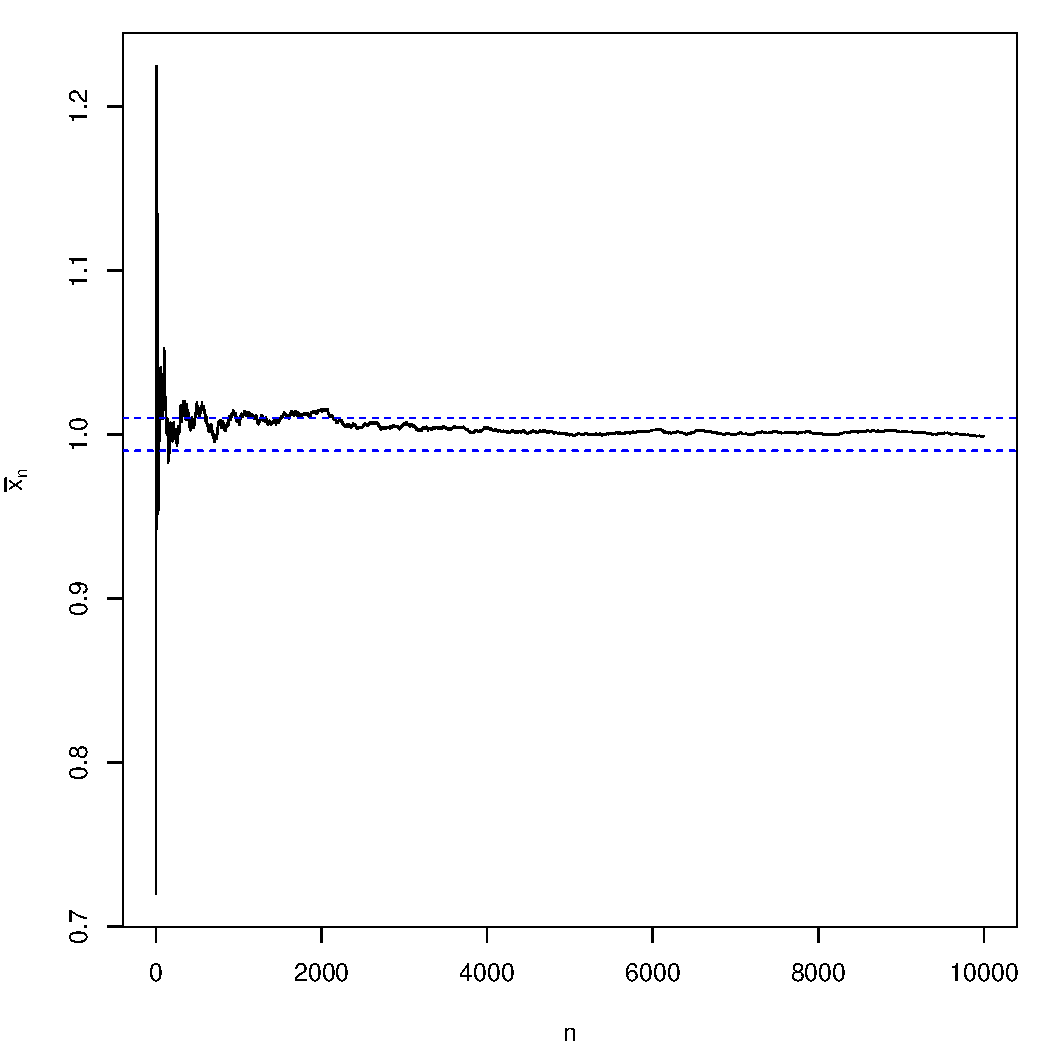
\includegraphics[width=10cm,height=10cm]{figure/CLT-normalplot-1} 

}


\end{knitrout}
\footnotesize
		\emph{Notes: This graphs shows the convergence of $\bar{X}$ as $n\to\infty$ for a normal distribution.}
	\end{minipage}
\end{figure}

From Figure \ref{fig:CLTnormal} we can see that $\overline{X}_n$ gets arbitrarily close to $\mu$ as $n$ increases indefinitely. In words, as the sample size $n$ increases, the sample mean converges to the theoretical mean. 
\end{example}

\begin{example}[Tossing a fair coin]
Now we simulate $n = 1000$ coin tosses. After each simulated toss, we plot the proportion $X_n$ of heads obtained so far against the number $n$ of tosses so far. The LLN says we should see a trace that gets very close to $1/2$ as $n$ increases.

In R, the code is:

\begin{knitrout}
\definecolor{shadecolor}{rgb}{0.969, 0.969, 0.969}\color{fgcolor}\begin{kframe}
\begin{alltt}
\hlcom{# Set up}
\hlkwd{set.seed}\hlstd{(}\hlnum{123}\hlstd{)}                            \hlcom{# set seed}
\hlstd{N} \hlkwb{<-} \hlnum{10000}                               \hlcom{# total number of tosses}
\hlstd{n} \hlkwb{<-} \hlnum{1}\hlopt{:}\hlstd{N}                                 \hlcom{# vector: n = 1, 2, ...., N; Toss number}

\hlcom{# Simulate and plot}
\hlstd{h} \hlkwb{<-} \hlkwd{rbinom}\hlstd{(}\hlkwc{n} \hlstd{= n,} \hlkwc{size} \hlstd{=} \hlnum{1}\hlstd{,} \hlkwc{prob} \hlstd{=} \hlnum{1}\hlopt{/}\hlnum{2}\hlstd{)} \hlcom{# vector: H = 0 or 1 each with p = 1./2}
\hlstd{x} \hlkwb{<-} \hlkwd{cumsum}\hlstd{(h)} \hlopt{/} \hlstd{n}                       \hlcom{# vector: proportion of heads}
\hlkwd{plot}\hlstd{(n, x,} \hlkwc{type} \hlstd{=} \hlstr{"l"}\hlstd{,} \hlkwc{ylim} \hlstd{=} \hlkwd{c}\hlstd{(}\hlnum{0}\hlstd{,} \hlnum{1}\hlstd{),} \hlkwc{ylab} \hlstd{=} \hlkwd{expression}\hlstd{(}\hlkwd{bar}\hlstd{(x)[n]))}
\hlkwd{abline}\hlstd{(}\hlkwc{h} \hlstd{=} \hlnum{0.52}\hlstd{,} \hlkwc{col} \hlstd{=} \hlstr{"blue"}\hlstd{,} \hlkwc{lty} \hlstd{=} \hlnum{2}\hlstd{)}
\hlkwd{abline}\hlstd{(}\hlkwc{h} \hlstd{=} \hlnum{0.48}\hlstd{,} \hlkwc{col} \hlstd{=} \hlstr{"blue"}\hlstd{,} \hlkwc{lty} \hlstd{=} \hlnum{2}\hlstd{)}
\end{alltt}
\end{kframe}
\end{knitrout}

\begin{figure}[H]
  \caption{Convergence of mean from binomial distribution}
    \label{fig:CLTbinomial}
     \centering
    \begin{minipage}{.9\linewidth}
\begin{knitrout}
\definecolor{shadecolor}{rgb}{0.969, 0.969, 0.969}\color{fgcolor}

{\centering 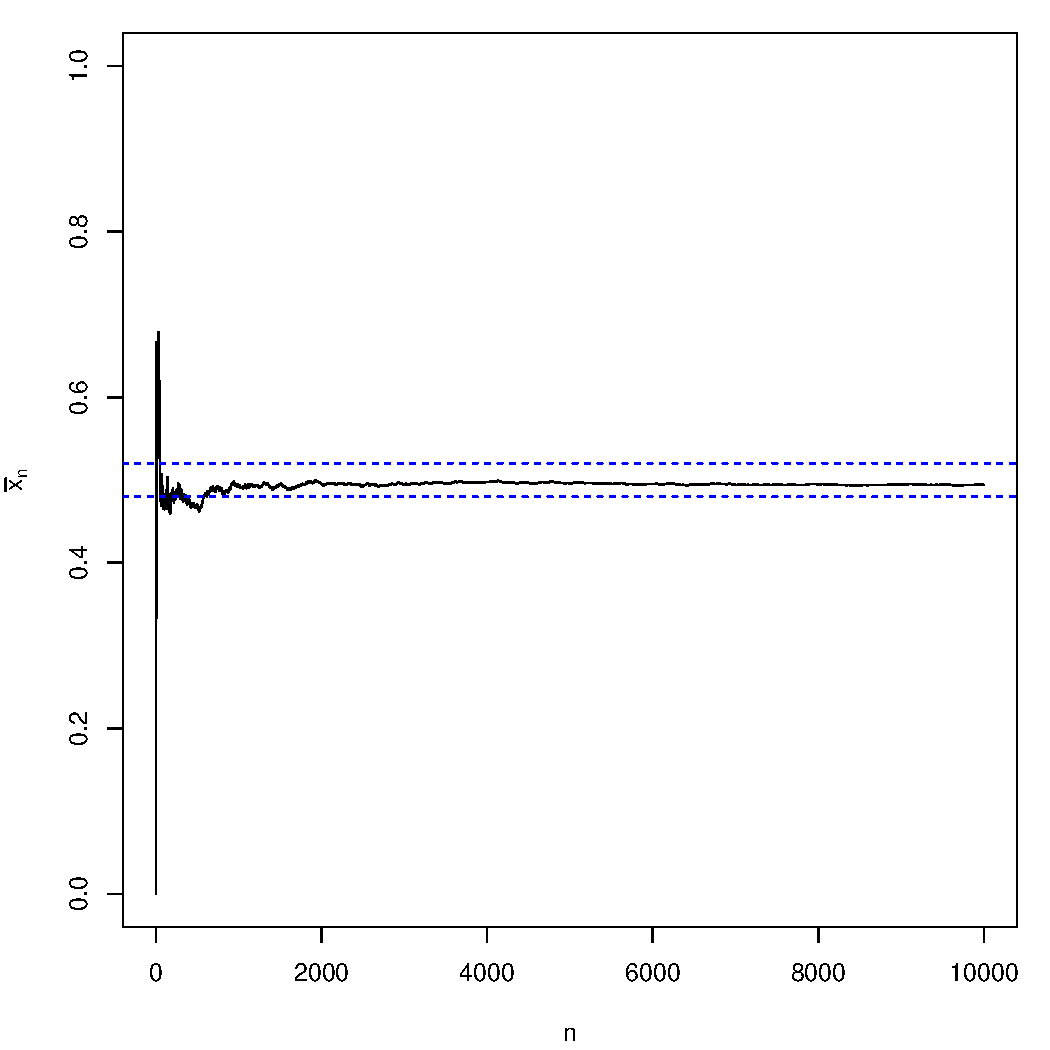
\includegraphics[width=10cm,height=10cm]{figure/CLT-binomialPlot-1} 

}


\end{knitrout}
\footnotesize
		\emph{Notes:} This graphs shows the convergence of $\bar{X}$ as $n\to\infty$ for a binomial distribution.
	\end{minipage}
\end{figure}

Note that the $n$th element of the vector \texttt{x} is the mean of the first $n$ elements of \texttt{h}. Figure \ref{fig:CLTbinomial} shows that the mean from a binomial distribution converges to the population mean $\mu = p = 1/2$, as $n\to \infty$. Note that the dashed lines at 0.48 and 0.52 illustrate the LLN with $\epsilon = 0.02$
\end{example}


Another important feature is that Khinchine's WLLN  is broader than Theorem \ref{teo:chebyshev} (Consistency of Unbiased Estimator), as \textbf{it does not require that the variance of the distribution be finite}. On the other hand, it is not broad enough, because most of the situations we encounter where we will need a result such as this will not involve i.i.d. random sampling. A broader LLN Theorem is the following:

\begin{theorem}[Chebychev's Weak Law of Large Numbers]\label{theorem:ChebychevWLLN}
  If $X_i, i = 1,...,n$ is a sample of observations such that $\E(X_i) = \mu_i <\infty$ and $\var(X_i)=\sigma^2_i < \infty$ such that
  
\begin{equation*}
  \frac{\bar{\sigma}^2_n}{n} = \frac{\sum_{i = 1}^n\sigma_i^2}{n^2}\to 0\quad \mbox{as $n\to\infty$},
\end{equation*}
%
then

\begin{equation*}
  \overline{X}_n - \bar{\mu}_n \pto 0.
\end{equation*}
\end{theorem}

The Chebychev's theorem does not state that $\overline{X}_n$ converges to $\bar{\mu}_n$, or even that it converges to a constant at all. The theorem states that as $n$ increases without bound, these two quantities will be arbitrarily close to each other. In other words, the difference between them converges to a constant, zero. The more important difference between the Khinchine and Chebyshev theorems is that the second allows for heterogeneity in the distributions of the random variables that enter the mean. This will be very useful in cases where the independence assumption may hold but the identical distribution assumption does not (such as random sampling with cross-sectional data). For example, the $X_i$'s may have different means and/or variances for each $i$. If we retain the independent assumption but relax the identical distribution assumption, then we can still get convergence of the sample mean.

It is important to stress that the behavior of the variance of $\overline{X}_n$ is the key element in this \textbf{LLN}. Independence implies that all covariances among the $X_i$ are zero, so that the variance of $\overline{X}_n$ simplifies to the sum of the variances of the $X_i$ divided by $n^2$. Then the key mechanism is that the variance of $\overline{X}_n$ converges to zero:

\begin{equation*}
 \lim_{n\to\infty}\var\left[ \overline{X}_n\right]=\lim_{n\to\infty}\frac{1}{n^2}\sum_{n=1}^n\var\left(X_i\right)=\lim_{n\to\infty}\frac{\sum_{i = 1}^n\sigma^2_i}{n}=0 
\end{equation*}

To illustrate Chebychev's WLLN we have created artificial data sets from independent normal distributions with different mean and standard deviations. Figure \ref{fig:chebychev} displays the sequence $\bar{X}_n - \bar{\mu}_n$ in black line and $\bar{\sigma}^2 / n^2$ as $n\to \infty$ in a red line. It can be observed that both sequences change with sample size, but as the number of observations increases both settle down to zero.  However, note that the sequence $\bar{X}_n - \bar{\mu}_n$ converges in probability, whereas $\bar{\sigma}^2 / n^2\to 0$ in a deterministic way. 


\begin{figure}[H]
  \caption{Chebychev's Convergence}
    \label{fig:chebychev}
         \centering
    \begin{minipage}{.9\linewidth}
\begin{knitrout}
\definecolor{shadecolor}{rgb}{0.969, 0.969, 0.969}\color{fgcolor}

{\centering 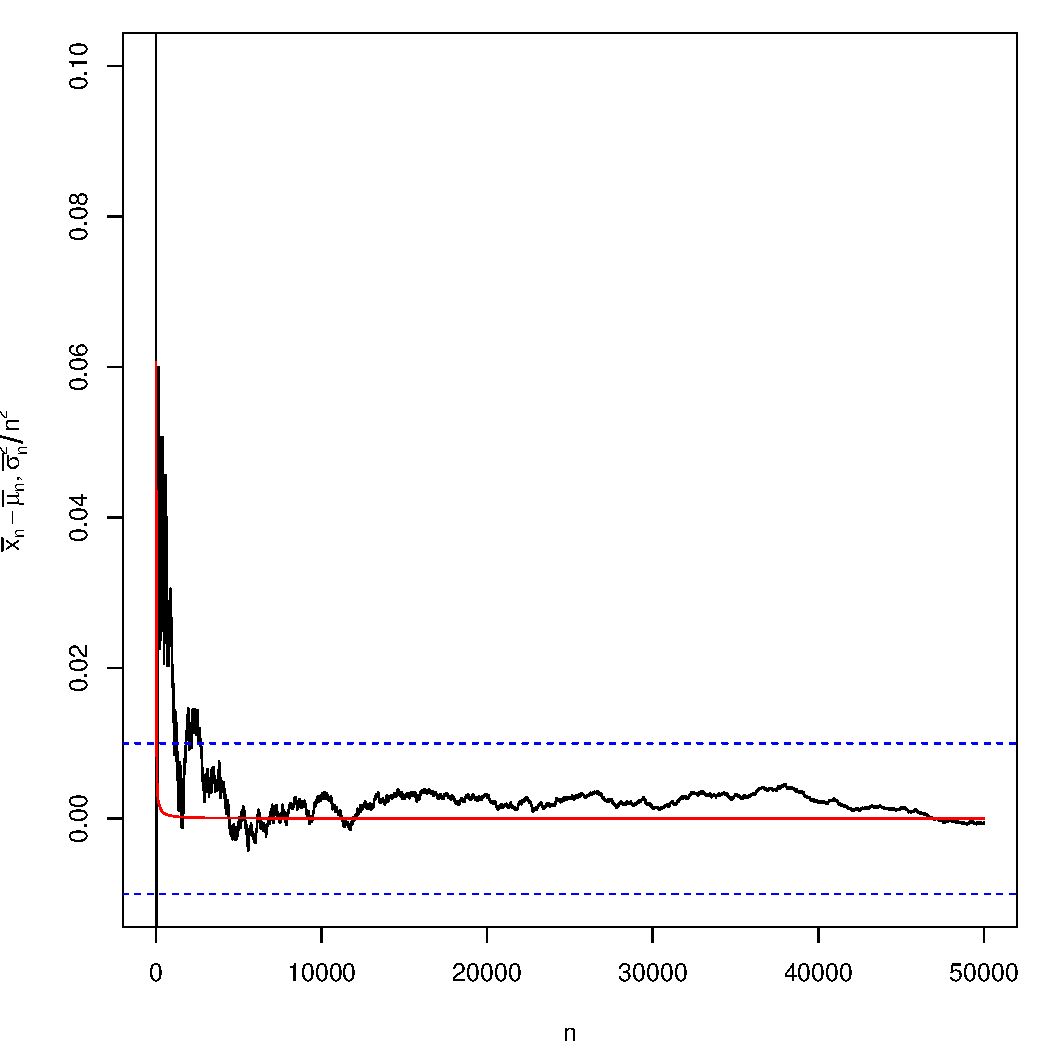
\includegraphics[width=10cm,height=10cm]{figure/cheby-convergence-1} 

}


\end{knitrout}
\footnotesize
		\emph{Notes: This graphs shows the convergence of $\bar{X}_n - \bar{\mu}_n$ and $\bar{\sigma}^2 / n^2$ as $n\to\infty$.}
	\end{minipage}
\end{figure}

\begin{remark}
  When the iid assumption is relaxed, stronger restrictions need to be place on the variances of each of the random variables. If some assumption are weakened then other assumptions must be strengthened. 
\end{remark}

To apply those LLN for several variables we have to know that summands of iid different random variables are also iid.

\begin{proposition}
	Let $\vg:\SR^K\to \SR^l$ be a continuous function. (i) Let $\mX_i$ and $\mX_t$ be identically distributed. Then $\vg(\mX_i)$ and $\vg(\mX_t)$ are identically distributed. (ii) Let $\mX_i$ and $\mX_t$ be independent. Then $\vg(\mX_i)$ and $\vg(\mX_t)$ are independent.
\end{proposition}

Therefore, using this proposition we can state the following proposition:

\begin{proposition}\label{proposition:iid_transf}
	If $\left\{(\mZ'_i,\mX_i,\vepsi_i)\right\}$ is an i.i.d random sequence, then $\left\{\mX_i\mX_i'\right\}$, $\left\{\mX_i\vepsi\right\}$, $\left\{\mZ_i\mX_i'\right\}$, $\left\{\mZ_i\vepsi_i\right\}$, and $\left\{\mZ_i\mZ_i'\right\}$ are also i.i.d sequences. 
\end{proposition}

This result is useful in situations in which we have observations from a random sample, as in a simple cross section. The result does not apply to stratified cross sections since there the observations are not identically distributed across strata, and generally will not apply to time-series data since there the observations $(\mX_i, \vepsi_i)$ generally are not independent. For these situations, we need laws of large numbers that do not  impose the i.i.d assumption.

What about expectations? The Jensen and Cauchy-Schwarz inequality will help us to work with Expectations of random variables. 

\begin{theorem}[Jensen's Inequality]\label{theorem:Jansen-Inequality}
If $g(X_n)$ is a concave function of $X_n$ then

\begin{equation*}
  g\left[\E(X_n)\right] \geq \E\left[g(X_n)\right]
\end{equation*}
\end{theorem}

\begin{theorem}[Cauchy-Schwarz Inequality]\label{theorem:Cauchy-Inequality}
For two random variables
\begin{equation*}
  \E\left[\left|X_nY_n\right|\right]\leq \left\lbrace \E\left[X_n^2\right]\right\rbrace^{1/2} \left\lbrace \E\left[Y_n^2\right]\right\rbrace^{1/2} 
\end{equation*}
\end{theorem}


%We can use this theorem in order to prove that the OLS variance estimator is consistent. Consider the i.i.d random variables $\epsilon_1^2, \epsilon_2^2, ..., \epsilon_N^2$, which have mean $\E\left[\epsilon_n^2\right] = \sigma^2$. From Khinchine's theorem it follows that:

%\begin{equation}
%\frac{1}{N}\sum_{i = 1}^N \epsilon_{i}^2 \pto \sigma^2
%\end{equation}

%which is the same as to say

%\begin{equation}
%\plim N^{-1}\vepsi'\vepsi = \sigma^2
%\end{equation} 

%To prove $\widehat{\sigma}^2 = \sigma^2$ consider the following estimator:

%\begin{eqnarray}
%\widehat{\sigma}^2 &=& \frac{\widehat{\vepsi}'\widehat{\vepsi}}{N - K}\nonumber \\
% & = & \frac{1}{N - K}\vepsi'\left(\mI - \mX\left(\mX'\mX\right)^{-1}\mX'\right)\vepsi \nonumber\\
% & = & \frac{N}{N - K}\left[\frac{\vepsi'\vepsi}{N} - \frac{\vepsi'\mX}{N}\left(\frac{\mX'\mX}{N}\right)^{-1}\frac{\mX'\vepsi}{N}\right]
%\end{eqnarray}

%Then, using Slutksy's theorem and the fact that $\plim \left[N/\left(N - K\right)\right] = 1$,

%\begin{eqnarray}
%\plim \widehat{\sigma}^2 & = & \plim \frac{\vepsi'\vepsi}{N} - \plim \frac{\vepsi'\mX}{N}\plim \left(\frac{\mX'\mX}{N}\right)^{-1}\plim \frac{\mX'\vepsi}{N} \\
%& = & \sigma^2 - 0 \cdot Q^{-1} \cdot 0 \\
%& = & \sigma^2
%\end{eqnarray}

%Before, we need the following theorems:

%\begin{theorem}[Chebychev's LLN]\label{theorem:Chebychev}
%Let $\left\lbrace X_n \right\rbrace$ be a sequence of i.i.d. random variables such that $\E\left[ X_n\right]$ and $\var\left[ X_n\right] $ exists $(n=1,2,3,...)$. Denote:

%\begin{equation*}
%E_N\left[X\right]\equiv \frac{1}{N}\sum_{n=1}^NX_n 
%\end{equation*}
%then $\E_N\left[X \right]\pto \E\left[ X\right]$ as $N\to\infty$
%\end{theorem}

%The behavior of the variance of $E_N\left[X \right]$ is the key element in this \textbf{LLN}. Independence implies that all covariances among the $X_n$ are zero, so that the variance of $\E_N\left[ X\right]$ simplifies to the sum of the variances of the $X_n$ divided by $N^2$. Then the key mechanism is that the variance of $\E_N\left[ X\right]$ converges to zero because the variance of the $X_n$ $(n-1,...,N)$ are all equal:

%\begin{equation*}
% \lim_{N\to\infty}\var\left[ \E_N\left[ X\right]\right]=\lim_{N\to\infty}\frac{1}{N^2}\sum_{n=1}^N\var[X]=\lim_{N\to\infty}\frac{\var[X]}{N}=0 
%\end{equation*}

%As a result, $\E_N[X]$ converges in distribution to the constant equal to its mean.


%==============================================
\section{Convergence in Distribution}
%==============================================


\begin{definition}[Convergence in Distribution]\label{definition:convergece_in_distribution}
	If the cdfs $F_{X_n}$ of the sequence of random variables $\left\lbrace X_n \right\rbrace $ converge to the cdf $F_{X}$ as $n\to \infty$ at all points $z$ where $F_{X}(z)$ is continuous, then $\left\lbrace X_n\right\rbrace $ converges in distribution to $X$. This will be denoted
	
	\begin{equation*}
	X_n\dto X
	\end{equation*}
%	
or 
	\begin{equation*}
	\lim_{n\to \infty}|F_{X_n}-F_{X}| = 0
	\end{equation*}
\end{definition}

This theorem states that the distribution of $X_n$ gets closer and closer to that of the random variable $X$, so that the distribution of $X$, the cdf $F_{X}$, can be used as an \textbf{approximation} to the distribution of $F_{X_n}$.  We can also say that $X$ es the \textbf{limiting distribution} of $X_n$.

%This statement is about the probability distribution associated with $X_n$; it does not imply that $X_n$ converges at all.

Convergence in distribution can be extended to random vectors and matrices although not in the element by element manner that we extended the earlier convergence forms. The reason is that convergence in distribution is a property of the CDF of the random variable, not the variable itself. Thus, $\vx_n\dto \vx$ if $\lim_{n\to \infty}|F_{\vx_n}-F_{\vx}| = 0$ and likewise for a random matrix. 


\begin{remark}
  One important case in which the limiting cdf $F$ is discontinuous is when $X$ is generate, meaning that it is identically equal to a constant $c$, so that $\Pr(X = c) = 1$. 
\end{remark}

\begin{remark}
In most applications, $X$ is either a normal or chi-square distributed random variable. 
\end{remark}


As an example, it is well know that 

\begin{equation*}
t_{n-1}\dto N(0, 1)
\end{equation*}

as $n\to \infty$.

\begin{theorem}[Convergence in probability implies convergence in distribution]\label{teo:pto_implies_dto}
  If the sequence of random variables $\left\lbrace X_n \right\rbrace$ convergences in probability to a random variable $X$, the sequence also converges in distribution to $X$. In other words:
  
  \begin{equation*}
    X_n\pto X\implies X_n\dto X
  \end{equation*}
\end{theorem}

Convergence in distribution is a weaker form of convergence than convergence in probability, in the sense that $\pto \implies \dto$. Intuitively, when $X_n$ converges to $X$ in probability as $n\to \infty$, the random variable $X_n$ will be arbitrarily close to random variable $X$ for $n$ sufficiently large. Therefore, the probability law of $X_n$ will be arbitrarily close to the probability law of $X$ for $n$ sufficiently large. That is, $X_n$ will converge in distribution to $X$ as $n\to \infty$.

However, $\dto$ does not imply $\pto$. When $\vx = \vtheta$ is a vector of constants the converse does hold. That is, it is also true that

\begin{equation*}
  \vx_n\dto \vtheta \implies \vx_n\pto \vtheta
\end{equation*}

In this case the limiting distribution of $\vx_n$ is degenerate since it collapses to the single point $\vtheta$.

\begin{example}[Defining Limiting Distribution Through Convergence in Probability]
Let $\left\lbrace Y_n\right\rbrace$ be defined by $Y_n = \left(2 + n^{-1}\right)X + 3$, where $X\sim \rN(1, 2)$. Using properties of $\plim$ operator if follows that

\begin{equation*}
  \plim \left(Y_n\right) = \plim \left[\left(2 + n^{-1}\right)X\right] + \plim(3) = 2X + 2 \sim \rN(5, 8). 
\end{equation*}
Then, Theorem \ref{teo:pto_implies_dto} implies that $Y_n\dto \rN(5, 8)$.
\end{example}

Another important result is that the moments of the asymptotic distribution of a random variable are not necessarily equal to the limits of the moments of the random variable's finite sample distribution. That is, in terms of the first two moments, $\vx_n\dto \vx$ does not necessarily imply that $\lim \E(\vx_n) = \E(\vx)$ and $\lim \E(\vx_n\vx_n') = \E(\vx\vx')$. For example, in simultaneous equation estimation, we frequently encounter estimator that do not possess finite moments of any order, but that, nevertheless, possess asymptotic distributions with well-defined moments.

\begin{example}
Consider a random sample $(y_1, y_2,...,y_n)$ from a normal distribution with mean $\mu \neq 0$ and variance $\sigma^2$. As an estimator for $\mu^{-1}$, the inverse of the sample mean $\bar{y}_n^{-1}$ is a natural choice. To establish its statistical properties we note that, from Khinchine's theorem, $\plim \bar{y}_n = \mu$, and then, from the continuous mapping theorem, $\plim \bar{y}_n^{-1} = \mu^{-1}$. Also because $\sqrt{n}(\bar{y}_n - \mu)\sim \rN(0, \sigma^2)$ for all $n$, it follows that

\begin{equation*}
  \sqrt{n}(\bar{y}_n - \mu)\dto \rN(0, \sigma^2)
\end{equation*}

Then, 

\begin{equation*}
  \sqrt{n}\left(\bar{y}_n^{-1} - \mu^{-1}\right)\dto \rN(0, \sigma^2\mu^{-4})
\end{equation*}

Thus the mean of the asymptotic distribution of $\bar{y}_n^{-1}$ is $\mu^{-1}$, but $\lim \E\left(\bar{y}_n^{-1}\right)\neq \mu^{-1}$ because it can be shown that $\E\left(\bar{y}_n^{-1}\right)$ does not exists. Note that this example also demonstrate that an estimator can be consistent, that is $\plim \bar{y}_n^{-1} = \mu^{-1}$, without its bias and variance going to zero as $n\to\infty$ ($\E\left(\bar{y}_n^{-1}\right)$ and $\var\left(\bar{y}_n^{-1}\right)$ do not exist.)
\end{example}

Some useful results that combine both probability and limiting distribution are as follows.

\begin{theorem}[Rules for limiting distribution]\label{teo:rules_dto}

Consider the following rules
\begin{enumerate}
  \item If $X_n\dto X$ and $Y_n\pto c$, then
      \begin{equation}\label{eq:rule_dtop}
         X_nY_n \dto cX
      \end{equation}
%
      which means that the limiting distribution of $X_nY_n$ is $cX$. Also, 
        \begin{equation}\label{eq:rule_dtop_2}
            X_n + Y_n \dto X + c
        \end{equation}
        
        \begin{equation}\label{eq:rule_dtop_3}
            X_n / Y_n \dto X / c, \quad \mbox{if $c\neq 0$}
        \end{equation}
        
    \item If $X_n\dto X$ and $g(X_n)$ is a continuous function, then
          \begin{equation}\label{eq:rule_dtop_4}
            g(X_n)\dto g(X)
          \end{equation}
    \item $\vx_n \dto \vx$, $\mA_n\pto \mA \implies \mA_n\vx_n \dto \mA\vx$, provided that $\mA_n$ and $\vx_n$ are conformable. In particular, if $\vx \sim \rN(\vzeros, \mSigma)$, then $\mA_n\vx_n\dto \rN(\vzeros, \mA\mSigma\mA')$.
    \item $\vx_n \dto \vx$, $\mA_n\pto \mA \implies \vx_n'\mA_n^{-1}\vx_n\dto \vx'\mA^{-1}\vx$, provided that $\mA_n$ and $\vx_n$ are conformable and $\mA$ is nonsingular.
\end{enumerate}
\end{theorem}

\begin{example}[Plims of Matrix Functions to Vector Random Variables]
Let $\left\lbrace \mX_n\right\rbrace$ and $\left\lbrace \mY_n\right\rbrace$ be such that $\plim\left(\mX_n\right) = \begin{pmatrix} 3 & 2 \\ 2 & 4 \end{pmatrix}$ and $\underset{(2\times 1)}{\mY_n}\dto\underset{(2\times 1)}{\mY}\sim \rN(\vzeros, \mI)$. Then, 

\begin{equation*}
  \mX_n\mY_n\dto \left[\plim\left(\mX_n\right)\right]\mY\sim \rN\left(\vzeros, \begin{pmatrix} 13 & 14 \\ 14 & 20\end{pmatrix}\right)
\end{equation*}

and

\begin{equation*}
  \mX_n^{-1}\mY_n\dto \left[\plim\left(\mX_n\right)\right]^{-1}\mY\sim \rN\left(\vzeros, \begin{pmatrix} .3125 & -.2188 \\ -.2188 & .2031\end{pmatrix}\right)
\end{equation*}
\end{example}

\begin{remark}
An useful example of Equation (\ref{eq:rule_dtop_4}) of Theorem \ref{teo:rules_dto} is the following. The exact distribution of $t_n^2$ is $F(1, n)$. But as $n\to \infty$, $t_n$ convergences to a standard normal variable. According to this result, the limiting distribution of $t_n^2$ will be that of the square of a standard normal, which is $\chi^2(1)$. Therefore, we conclude that:

\begin{equation*}
  F(1, n)\dto \chi^2(1)
\end{equation*}
\end{remark}


\begin{lemma}[Asymptotic Equivalence]\label{lemma:asymptotic_equiv}
  If $Y_n - X_n\pto 0$ and $X_n\dto X$ as $n\to \infty$, then $Y_n\dto X$
\end{lemma}

Intuitively, if two random variables $Y_n$ and $X_n$ are very close with probability approaching one as $n\to \infty$, they will follow the same large sample probability distribution. This lemma is very useful when one is interested in deriving the asymptotic distribution of $Y_n$. We can establish the asymptotic the asymptotic equivalence (in probability) between $Y_n$ and $X_n$ in the sense that $Y_n - X_n\pto 0$ as $n\to \infty$, then the asymptotic distributions of $Y_n$ and $X_n$ will be identical.\footnote{For example, this lemma is useful when deriving the distribution of spatial GLS is the same as the spatial FGSL. } 

\begin{theorem}[Cramer-Wold device]
If $\vx_n \dto \vx$, then $\vc'\vx_n \dto \vc'\vx$ for all conformable vectors $\vc$ with real valued elements.
\end{theorem}

%%%%%%%%%%%%%%%%%%%%%%%%%%%%%%%%%%%%
\section{Central Limit Theorems}
%%%%%%%%%%%%%%%%%%%%%%%%%%%%%%%%%%%%

Recall that we are interested in a way to describe the statistical properties of estimators when their exact distribution are unknown. However the previous tools do not allow us to find the limiting distribution. From Theorem \ref{teo:pto_implies_dto} (Convergence in probability implies convergence in distribution), we know that:

\begin{equation*}
  \widehat{\vtheta}_n\pto \vtheta \implies \widehat{\vtheta}\dto \vtheta.
\end{equation*}

That is, the limiting distribution of $\widehat{\vtheta}_n$ is a spike (the asymptotic distribution of $\widehat{\theta}_j$ collapses to a single point) and not very informative. The `trick' is to apply some normalization. For example, whereas $\widehat{\vtheta}_n\pto \vtheta$, we often find that

\begin{equation}
z_n = \sqrt{n}(\widehat{\vtheta}_n - \vtheta) \dto f(z),
\end{equation}
%
where $f(z)$ is a well-defined distribution with mean and positive variance. An estimator which has this properly is said to be \textbf{root-n consistent}.

\begin{mynote}
When learning econometrics is very difficult to understand how a estimator $\widehat{\theta}_n$ (random variable) converge to a single number but also converge to a (degenerate) distribution. We will see that under certain conditions $\widehat{\theta}_n$ converges in probability to $\theta_0$. This means that by choosing a large enough sample size $n$, the estimator will be as close as we want to the true parameter, with the probability of it being farther away as small as we want. Furthermore if we plot the distribution (or histogram) of $\widehat{\theta}_n$ for several $n$, it will eventually be just a spike centered on $\theta$ and not a normally distributed random variable. This is so because the variance of $\widehat{\theta}_n$ will go to zero eventually for a large enough $n$. Therefore, because $\var(\widehat{\theta}_n)\to 0$ the distribution shrink as $n\to \infty$. However, what does converge to a normally distributed random variable is $\sqrt{n}(\widehat{\theta}- \theta)$ because its variance does not grow with $n$. 
\end{mynote}

Central limit theorems, establish that, under some conditions, the arithmetic mean of a sufficiently large number of independent random variables, each with a finite expected value and finite variance, will be approximately normally distributed, regardless of the underlying distribution. 

The following Theorem gives the most classical (Central Limit Theorem) CLT. 


\begin{theorem}[Lindberg-Levy CLT (Univariate)]\label{theorem:LL_CLT_U}
Let $\left\lbrace X_n \right\rbrace$ be a sequence of i.i.d. random variables such that $\E(X_n) = \mu$ and the variance is strictly positive and finite, $0 < \sigma^2 < \infty$. Define $\overline{X}_n = n^{-1}\sum_{i = 1}^nX_i$. Then the distribution of

\begin{equation*}
  \begin{aligned}
      Z_n & = \frac{\overline{X}_n  - \E(\overline{X}_n)}{\sqrt{\var(\overline{X}_n)}} \\
          & = \frac{\overline{X}_n - \mu}{\sigma / \sqrt{n}} \\
      & = \frac{\sqrt{n}(\overline{X}_n - \mu)}{\sigma} \dto \rN(0, 1)
  \end{aligned}
\end{equation*}
%
as $n$ approaches infinity. This is the same as:
 
 
 \begin{equation*}
  \sqrt{n}(\overline{X}_n - \mu) = \frac{1}{\sqrt{n}}\sum_{i = 1}^n(X_i - \mu)\dto \rN(0, \sigma^2)
 \end{equation*}
\end{theorem}

This theorem tell us that if a large random sample is taken from any population distribution with finite variance, regardless of whether this population distribution is discrete or continuous, then the distribution of the standardized sample mean

\begin{equation*}
Z_n = \frac{\sqrt{n}(\overline{X}_n - \mu)}{\sigma}
\end{equation*}
%
will approximately follow a \rN(0, 1). Therefore, for each finite $n$, the distribution of $\overline{X}_n$ will be approximately a $\rN(\mu, \sigma^2/n)$.\\

It is important to stress that CLT does not say that a large population is approximately normally distributed. It says nothing about the distribution of the population; it is only a statement about the approximate distribution of a standardized sample mean $Z_n$. 

\begin{remark}
  Sometimes CLT is interpreted incorrectly as implying that the distribution of $\overline{X}_n$ approaches a normal distribution as $n\to \infty$. This is incorrect because $\var(\overline{X}_n)\to 0$ and $\overline{X}_n$ converges to a degenerate distribution $F(\cdot)$ such that $F(x) = 0$ if $x < \mu$ and $F(x) = 1$ if $x\geq \mu$.
\end{remark}

Multivariate versions of the CLTs can be obtained where each individual $\vx_i$ is a random vector in $\SR^K$, 


\begin{equation*}
\vx_i =\begin{pmatrix}
        x_{i1}\\
        x_{i2} \\
        \vdots\\
        x_{iK}
      \end{pmatrix}  
\end{equation*}
%
with mean vector:

\begin{equation*}
\vmu = \E(\vx_i) = \begin{pmatrix}
          \mu_1 \\
          \mu_2 \\
          \vdots \\
          \mu_K
       \end{pmatrix},
\end{equation*}
%
and covariance matrix $\mQ$. Then the sum of the random vectors will be componentwise, that is:

\begin{equation*}
\begin{pmatrix}
        x_{11}\\
        x_{12} \\
        \vdots\\
        x_{1K}
      \end{pmatrix} +
\begin{pmatrix}
        x_{21}\\
        x_{22} \\
        \vdots\\
        x_{2K}
      \end{pmatrix}+
\hdots +
\begin{pmatrix}
        x_{n1}\\
        x_{n2} \\
        \vdots\\
        x_{nK}
      \end{pmatrix} =
\begin{pmatrix}
\sum_{i = 1}^n x_{i1} \\
\sum_{i = 1}^n x_{i2} \\
\vdots \\
\sum_{i = 1}^n x_{iK}
\end{pmatrix}=
\sum_{i = 1}^n\vx_i.
\end{equation*}

The multivariate version of Theorem \ref{theorem:LL_CLT_U} is the following:


\begin{theorem}[Multivariate Lindberg-Levy CLT]\label{theorem:LL_CLT_M}
Let $\left\lbrace \vx_n \right\rbrace$ be a sequence of i.i.d. random variables from a multivariate distribution. If $\E(\vx_n) = \vmu$ and finite and positive covariance matrix $\mQ$. Then the distribution of

\begin{equation*}
  \begin{aligned}
      Z_n & = \sqrt{n}(\overline{\vx}_n - \vmu) \dto \rN(\vzeros, \mQ), 
  \end{aligned}
\end{equation*}
%
as $n$ approaches infinity, where $\overline{\vx}_n = (1 / n)\sum_{i = 1}^n\vx_i$.
\end{theorem}

The Linderbeg-Levy CLT is one of the several forms of this extremely powerful result. An important extension allow us to relax the assumption of equal variances. The Linderberg-Feller CLT allows for this extension:

\begin{theorem}[Univariate Lindberg-Feller CLT]\label{theorem:LF_CLT_U}
Let $\left\lbrace X_n\right\rbrace, i = 1, 2,...,n$ be a sequence of i.i.d. random variables. If $\E(X_i) = \mu_i$ and the variance is strictly positive and finite, $0 < \sigma^2_i < \infty$. Define 

\begin{equation*}
  \bar{\mu}_n = \frac{1}{n}(\mu_1 + \mu_2 + ... +\mu_n), \quad \mbox{and} \quad \bar{\sigma}^2_n =\frac{1}{n}(\sigma^2_1 + \sigma^2_2 + ... +\sigma^2_n)
\end{equation*}

If no single term dominates this average variance, which we could state as

\begin{equation*}
\lim_{n\to \infty} \frac{\max (\sigma_i)}{n \bar{\sigma}_n} = 0,
\end{equation*}
%
and if the average variance converges to a finite constant,

\begin{equation*}
\lim_{n\to \infty} \bar{\sigma}^2_n = \bar{\sigma}^2
\end{equation*}
%
then

\begin{equation*}
  \begin{aligned}
      Z_n &  = \frac{\sqrt{n}(\overline{X}_n - \bar{\mu})}{\bar{\sigma}} \dto \rN(0, 1)
  \end{aligned}
\end{equation*}
%
 as $n$ approaches infinity.
\end{theorem}

In practical terms, the theorem states that sums of random variables, regardless of their form, will tend to be normally distributed. 


\begin{theorem}[Multivariate Lindberg-Feller CLT]\label{theorem:LF_CLT_M}
Suppose that $\vx_1, \vx_2,...,\vx_n$ are a sample of random vectors such that $\E(\vx_i) = \vmu_i$, $\var(\vx_i) = \mQ_i$, and all mixed third moments of the multivariate distribution are finite. Let

\begin{equation*}
  \bar{\vmu}_n = \frac{1}{n}\sum_{i = 1}^n\vmu_i,
\end{equation*}

\begin{equation*}
  \overline{\mQ}_n = \frac{1}{n}\sum_{i = 1}^n\mQ_i.
\end{equation*}

We assume that

\begin{equation*}
  \lim_{n \to \infty}\overline{\mQ}_n  = \mQ,
\end{equation*}
%
where $\mQ$ is a finite, positive definite matrix, and that for every $i$,

\begin{equation*}
  \lim_{n \to \infty}(n\overline{\mQ}_n)^{-1}\mQ_i = \lim_{n \to \infty}\left(\sum_{i = 1}^n \mQ_i\right)^{-1} \mQ_i = \vzeros
\end{equation*}

We allow the means of the random vectors to differ, although in the cases that will analyze, they will generally be identical. The second assumption states that individual components of the sum must be finite and diminish in significance. There is also an implicit assumption that the sum of matrices is nonsingular. Because the limiting matrix is nonsingular, the assumption must hold for large enough $n$, which is all that concerns us here. With these in place, the result is

\begin{equation*}
  \sqrt{n}(\bar{\vx}_n - \bar{\vmu}_n)\dto \rN(\vzeros, \mQ)
\end{equation*}
\end{theorem}

\begin{theorem}[Liapounov Central Limit Theorem]
Suppose that $\left\lbrace X_n\right\rbrace, i = 1, 2,...,n$ is a sequence of independent random variables with finite mean $\mu_i$ and finite positive variances $\sigma^2_i$ such that $\E\left[\left|X_i - \mu_i\right|^{2 + \delta}\right]$ if finite for some $\delta > 0$. If $\bar{\sigma}_n$ is positive and finite for all $n$ sufficiently large, then

\begin{equation*}
  \frac{\sqrt{n}(\overline{X}_n - \bar{\mu}_n)}{\bar{\sigma}_n}\dto\rN(0, 1)
\end{equation*}
\end{theorem}

This version of the central limit theorem requires only that moments slightly larger than two be finite and it is generally used when the variables are fixed. 

We end this section by defining the concept of \textbf{asymptotic variance}.


\begin{definition}[Asymptotic Variance]\label{def:asymptotic_variance}
Let $\left\lbrace\vx_n\right\rbrace$ be a sequence of random vectors. If there exists a sequence of matrices $\left\lbrace \mV_n\right\rbrace$ such that $\mV_n$ is nonsingular for all $n$ sufficiently large and $\mV^
{-1/2}\vx_n \adistr \rN(\vzeros, \mI)$, then $\mV_n$ is called the asymptotic covariance matrix of $\vx_n$, denoted $\avar(\vx_n)$.
\end{definition}


%-----------------------------------
\section{Orden in Probability}
%-----------------------------------


Similarly to the nonsthocastic sequences, we can make similar statement about $o$ and $O$ when we have random variables. The following theorem state the definition of unboudedness and convergence for random variables: 

\begin{definition}[Order in Probability]\label{definition:order_prob}
Consider the following two definition:

\begin{enumerate}
		\item \textbf{Stochastically Bounded (Big O)}: The sequence of random variables  $\left\{X_n\right\}$ is at most of order in probability $n^\lambda$, and we write
		
		\begin{equation}
			X_n = O_p(n^\lambda)
		\end{equation}
		
		if, for every $\epsilon > 0$, there exists a real number $n_0$ such that:
		
		\begin{equation}
			\Pr\left[n^{-\lambda} \left|X_n \right| \geq n_0 \right]\leq \epsilon
		\end{equation}
		
		for all $n$. 
		
		\item \textbf{Stochastic Convergence}: Also, we say that $\left\{X_n\right\}$ is of smaller order in probability than $n^\lambda$ and we write
		
		\begin{equation}
		X_n = o_p\left(n^\lambda\right)
		\end{equation}
		
		if 
		
		\begin{equation}
			\plim n^{-\lambda}X_n = 0
		\end{equation}
		
		When $\lambda = 0$, $X_n$ converges to zero, and we also write $X_n=o_p(1)$.
		
	\end{enumerate}
\end{definition}

Intuitively, for $X_n = O_p(n^\lambda)$ with $\lambda > 0$, the order $n^\lambda$ is the fastest growth rate at which $X_n$ goes to infinity with probability approaching 1. When $\lambda < 0$, the order $n^\lambda$ is the fastest convergence rate at which $X_n$ vanishes to 0 with probability approaching 1. Thus, $X_n= O_p(1) = O_p(n^0)$ implies that for $n$ sufficiently large, $\left|X_n\right|$ takes value larger than a very large constant has a tiny probability. In other words, $\left|X_n\right|$ is bounded by a constant with a very high probability for all $n$ sufficiently large. 

\begin{definition}[Stochastically Negligible]
	If $X_n\pto 0$, then $X_{n} = o_p(1)$. If $X_n = n^\lambda o_p(1)$, then $X_n = o_p(n^{-\lambda})$	
\end{definition}

To give some intuition about these definitions, consider $\vx_n \dto \vx$ and $\vy_n\pto \vzeros$. Then:

\begin{equation*}
  \vx_n + \vy_n \dto \vx\quad \mbox{by \ref{eq:rule_dtop} in Theorem \ref{teo:rules_dto}}
\end{equation*}

That is, if  $\vz_n = \vx_n + \vy_n$ and $\vy_n\pto \vzeros$, implying that $\vz_n - \vx_n \pto \vzeros$, then the asymptotic distribution of $\vz_n$ is the same as that of $\vx_n$. Note that this is the same as Lemma \ref{lemma:asymptotic_equiv} (asymptotic equivalence). So we can write:

\begin{equation*}
  \vz_n \adistr \vx_n\quad \mbox{or}\quad \vz_n = \vx_n + o_p(1)
\end{equation*}
%
where $o_p(1)$ is some variable ($\vy_n$ in this case) that is sthochastically negligible, that is, it converges to zero in probability. 

This is more intuitive if we think in the consistency of OLS estimator. Given the OLS consistency, it is the same to write:

\begin{equation*}
\widehat{\vbeta}_n \pto \vbeta_0\quad \mbox{as $n\to\infty$}
\end{equation*}
%
as

\begin{equation*}
\widehat{\vbeta}_n = \vbeta_0  + o_p(1) \quad \mbox{as $n\to\infty$}
\end{equation*}

In other words, a consistent estimator is equal to the true estimator plus something that converges to 0 in probability. 

%------------------------------------------------------------------
\begin{lemma}[Convergence in distribution implies boundedness]
  Let $X_n$ be a random variable with CDF $F_n(\cdot)$, and let $X$ be a random variable with continuous CDF $F(\cdot)$. If $X_n\dto X$ as $n\to \infty$, then $X_n = O_p(1)$
\end{lemma}
%------------------------------------------------------------------

Intuitively, if the probability distribution of $X_n$ converges to a well-defined continuous probability distribution as $n\to \infty$, then $X_n$ is bounded in probability. This result is very useful for establishing that a sequence of random variables is bounded in probability. Often it is easier to verify that a sequence of random variables converges in distribution. 

When do we use the $O_p$?  If a random vector converges in distribution $\vx_n \dto \vx$ (for example $\vx\sim \rN(\vzeros, \mV)$) then $\vx_n = O_p(1)$. 

\begin{example}
  If $X_n\sim N(0,1)$ for all $n\geq 1$. Then $X_n = O_p(1)$ because for any given $\delta > 0$, there exists a finite constant $M = \Phi^{-1}(1 - \delta/2)<\infty$, where $\Phi$ is the $\rN(0, 1)$ CDF, such that
  
  \begin{equation*}
    \Pr(\left|X_n\right| > M) = 2\left[1 - \Phi(M)\right] = \delta < 2\delta
  \end{equation*}
  %
  for all $n \geq 1$
\end{example}

$O_p(1)$ is weaker than $o_p(1)$ in the sense that $X_n = o_p(1)$ implies $X_n = O_p(1)$ but not the reverse.

There are many simple rules for manipulating $o_p(1)$ and $O_p(1)$ sequences which can be deduced from the continuous mapping theorem or Slutsky's Theorem. For example:

\begin{eqnarray*}
 o_p(1) + o_p(1) & = & o_p(1) \\
 o_p(1) + O_p(1) & = & O_p(1) \\
 O_p(1) + O_p(1) & = & O_p(1) \\
 o_p(1) o_p(1)   & = & o_p(1) \\
 o_p(1) O_p(1)   & = & o_p(1) \\
 O_p(1) O_p(1)   & = & O_p(1)
\end{eqnarray*}

One of the most common uses of this concept of stochastic order is ``root-$n$'' $(\sqrt{n})$ consistency:

\begin{definition}[$\sqrt{N}$-Consistent]
		if $\sqrt{n}\left(\vtheta_n - \vtheta_0\right)= O_p(1)$, then $\vtheta_n$ is $\sqrt{n}$ consistent for $\vtheta_0$
\end{definition}

\begin{example}[OLS and $O_p$ and $o_p$]
Recall that:

\begin{equation*}
  \widehat{\vbeta}_n = \vbeta_0 + (\mX'\mX)^{-1}\mX'\vepsi.
\end{equation*}

Under appropriate assumption, we know that:

\begin{equation*}
  \frac{1}{n}\mX'\mX\pto \E(\mX'\mX),
\end{equation*}
%
which is finite and positive definite. The fact that the elements of $n^{-1}\mX'\mX$ converge to finite limits in probability implies that $N^{-1}\mX'\mX$ is \textbf{bounded} in the sense that the sequences of the elements within $n^{-1}\mX'\mX$ are bounded, and under these circumstances we say that $\mX'\mX$ is at most of order $n$, that is, $\mX'\mX = O_p(n)$, or we can say:

\begin{equation*}
n^{-1}\mX'\mX = O_p(1).
\end{equation*}

We also assume that $n^{-1/2} \mX'\vepsi$ has probability limit which a normally distributed random variable with expectation zero and finite variance. So, we can write:

\begin{equation*}
\mX'\vepsi = O_p(n^{1/2}).
\end{equation*}

Thus:


\begin{equation*}
  \begin{aligned}
\widehat{\vbeta}_n - \vbeta_0 & =  (\mX'\mX)^{-1}\mX'\vepsi  \\
\widehat{\vbeta}_n - \vbeta_0 & =  (n^{-1}\mX'\mX)^{-1}n^{-1}\mX'\vepsi  \\
\widehat{\vbeta}_n - \vbeta_0 & = O_p(1) \cdot o_p(1) \\
\widehat{\vbeta}_n - \vbeta_0 & = o_p(1)
\end{aligned}
\end{equation*}

Also:

\begin{equation*}
  \begin{aligned}
\widehat{\vbeta}_n - \vbeta_0 & =  (\mX'\mX)^{-1}\mX'\vepsi  \\
\widehat{\vbeta}_n - \vbeta_0 & =  \left[O_p(n)\right]^{-1}O_p(n^{1/2}) \\
\widehat{\vbeta}_n - \vbeta_0 & =  O_p(n^{-1})O_p(n^{1/2}) \quad \because \left[O_p(n)\right]^{-1}= O_p(n^{-1})\\
\widehat{\vbeta}_n - \vbeta_0 & =  O_p(n^{-1/2})\\
\end{aligned}
\end{equation*}
%

So, we might then say that $\widehat{\vbeta}_n - \vbeta_0$ is converging to zero at the rate $1/\sqrt{n}$; and the rate tell us what multiplier of the variable $\widehat{\vbeta}_n - \vbeta_0$ stabilizes it so that it convergences to a well-defined random variables rather than to 0 or $\infty$. 

Note also that: 

\begin{equation*}
  \begin{aligned}
    \sqrt{n}(\widehat{\vbeta}_n - \vbeta_0) & =  n^{1/2}O_p(n^{-1})O_p(n^{1/2})\\
    & = n^{1/2} O_p(n^{-1/2}) \\
    & = O_p(1) \quad \because X_n = O_p(1/\sqrt{n}) \implies X_n / (1/\sqrt{n})= \sqrt{n} X_n = O_p(1) 
  \end{aligned}
\end{equation*}
\end{example}

\begin{example}[Rate of convergence for sample mean]
Consider and iid random sample $X_i$ with mean $\mu = 0$ and variance $\sigma^2 = 0,25$. Then, by the CLT the sample mean $\bar{X}$ we know that $\sqrt{n}(\bar{X}-\mu) /\sigma \dto \rN(0 , 1)$. That is, $\sqrt{n}(\bar{X}-\mu)/\sigma = O_p(1)$. This implies that $\bar{X} - \mu= O_p(\sqrt{n})$. Figure \ref{fig:Op_example} shows how $\bar{X}$ converges towards $\mu$ to the speed of $1\sqrt{n}$.
\end{example}


\begin{figure}[H]
  \caption{Convergence of the sample mean and speed of convergence}
    \label{fig:Op_example}
        \centering
    \begin{minipage}{.9\linewidth}
\begin{knitrout}
\definecolor{shadecolor}{rgb}{0.969, 0.969, 0.969}\color{fgcolor}

{\centering 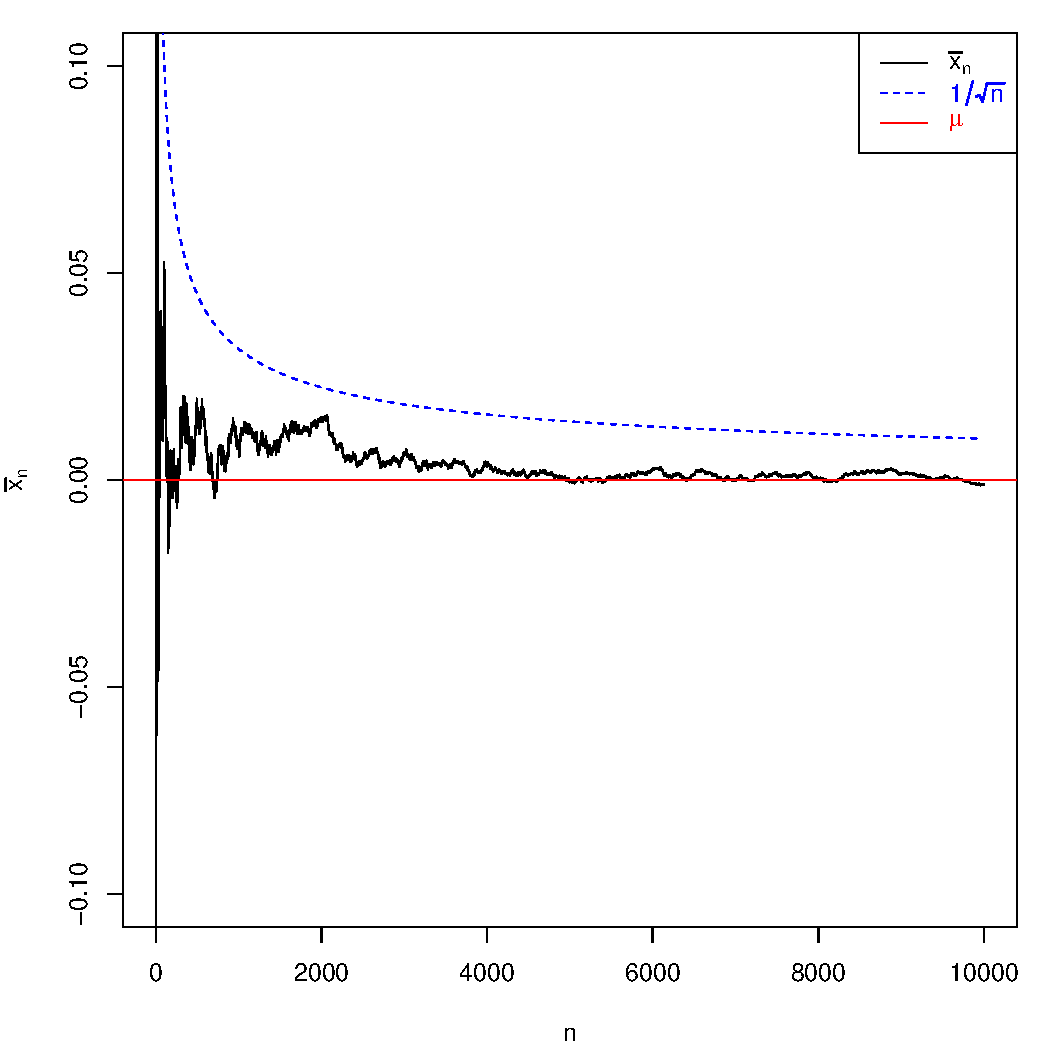
\includegraphics[width=10cm,height=10cm]{figure/CLT-normalplot-bigO-1} 

}


\end{knitrout}
\footnotesize
		\emph{Notes: This graphs shows the convergence of $\bar{X}$ to $\mu$ as $n\to\infty$ for a normal distribution as fast as $1/\sqrt{n}$.}
	\end{minipage}
\end{figure}

%----------------------------------
\section{Triangular Arrays}\label{sec:triangular-array}
%----------------------------------

An important question is the context of asymptotic theory is the following: \emph{What is the meaning of $n\to \infty$ in a spatial context?} Will increase the geographical area or will increase the number of spatial unit in a given geographical area? 

For spatial data, two distinct asymptotic frameworks have been studied: \textbf{increasing domain} and \textbf{infill asymptotic}. Increasing domain consists of a sampling structure where new observations (spatial units) are added at the edges (boundary points), similar to the underlying asymptotic in time series analysis. That is, increasing domain asymptotic refers to more and more observations being sampled over an increasing domain. The problem here is what the boundary is. When referring to increasing domain asymptotic, it is assumed that the spatial locations of the observations do not become dense. Infill asymptotic are appropriate when the spatial domain is bounded, and new observations (points) are added in between existing ones, generating denser surface. In most applications of spatial econometric, the implied structure is that of an increasing domain. 

The increasing domain framework requires the knowledge of \textbf{triangular arrays}.  The following definition give us a simply definition of Triangular Arrays. 

\begin{definition}[Triangular Array of Random Variables]\label{def:triangular-array} 
The ordered collection of random variables 

\begin{equation*}
\left\lbrace X_{11}, X_{21}, X_{22}, X_{31}, X_{32}, X_{33}, ... , X_{nn}, ...\right\rbrace,
\end{equation*}
%
or

\begin{equation*}
\begin{pmatrix}
X_{11} &        &        &        &        &        & \\
X_{21} & X_{22} &        &        &        &        & \\
X_{31} & X_{32} & X_{33} &        &        &        & \\
\vdots & \vdots & \vdots & \ddots &        &        & \\
X_{n1} & X_{n2} & X_{n3} & X_{n4} & \hdots & X_{nn} & \\
\vdots & \vdots & \vdots & \vdots & \vdots & \vdots & \ddots
\end{pmatrix}
\end{equation*}

is called a triangular array of random variables, and will be denoted by $\left\lbrace X_{nn}\right\rbrace$.
\end{definition}

Central limit theorems that are applied to triangular arrays of random variables are concerned with limiting distributions of appropriately defined function of the row average $S_n = n^{-1}\sum_{i = 1}^nX_{ni}$. For example, for $n = 3$ (third row) we have $S_3 = (1/3)(X_{31} + X_{32} + X_{33})$.  Note that the traditional CLTs deal with functions of average of the type $n^{-1}\sum_{i = 1}^n X_i$, the $X_i$'s being elements of the sequence $\left\lbrace X_n\right\rbrace$. However, the triangular array $\left\lbrace X_{nn}\right\rbrace$ is more general than a sequence $\left\lbrace X_n\right\rbrace$ in the sense that the random variables in a row of the array need not be the same as random variables in other rows. Thus, the triangular nature of a random variable leads to certain statistical problems, especially with respect to the relevant CLT that should be applied. In other words, we will need a CLT applicable to triangular array. Both the LLN and CLT require slightly stronger conditions than the LLN and CLT for i.i.d sequence of random variables. 

What are the conditions on the random variables so that a properly $S_n$ converges to a normal distribution as $n\to \infty$. In a nutshell, assume: 

\begin{itemize}
  \item Independence: assume all random variables in the array are independent.
  \item Centering: assume $\E(X_{j,i}) = 0$ for all $j, i$.
  \item Variances converge: assume $\sum_{i = 1}^n\E(X_{n, i}^2)\to \sigma^2> 0$ as $n\to\infty$
  \item No single variance is too large.
\end{itemize}

Then $S_n \dto N(0, \sigma^2)$ as $n\to\infty$.

Probably you're asking yourself, why triangular arrays are important in the spatial context? Note that if we adopt the increasing domain approach, it is clear that as $n$ increases,  $\mW$ itself changes as observations are added. To see this,  let $\vtheta_0 = (\vbeta_0^\top, \rho_0, \sigma_0^2)^\top$ be the true parameter vector. We further assume that variables and estimates depend on the sample size $n$. This will allow us to study their behavior as $n\to \infty$.  Therefore, denote $\mA_n(\rho) = \mI_n - \rho \mW_n$ for any value of $\rho$. The ``equilibrium'' vector is

\begin{equation}\label{eq:equilibrium_slm}
\vy_n = \mA_n^{-1}(\mX_n\vbeta_0 + \vepsi_n)
\end{equation}
%
where $\mA_n = \mA_n(\rho_0)$ is nonsingular. Let $\vepsi_n(\vdelta) = \vy_n - \mX_n\vbeta - \rho \mW_n\vy_n$, where $\vdelta = (\vbeta^\top, \rho)^\top$. Thus, $\vepsi_n = \vepsi_n(\vdelta_0)$. Since the matrices $(\mI_n - \rho\mW)^{-1}$ generally depend upon the sample size $n$, the vectors $\vy$ and $\vepsi$ will also depend upon $n$, and they will form a \textbf{triangular arrays}. This is due to the fact that for the ``boundary'' elements the sample weights matrix changes as new spatial units --- or new data points --- are added. That is, new spatial units change the structure for the existing spatial units \citep[see for example][]{kelejian1999generalized, kelejian2001asymptotic, anselinSpatialEcon}. For example, the outcome for the first spatial unit, $y_{1,n}$, will be different if we consider a total  $n = 10$ or $n = 15$ observations because of the changing nature of $\mW$ as $n$ changes and given the DGP in Equation (\ref{eq:equilibrium_slm}). This implies that these elements and the vector $\vy$ should be indexed by $n$:

\begin{equation*}
  \vy_n = (y_{11}, y_{21}, y_{22},..., y_{nn})
\end{equation*}

For example, for $n = 1, 2, 3$, then (by row):

\begin{equation*}
\begin{aligned}
  n = 1 & \implies y_{11} \;         \\
  n = 2 & \implies y_{12} \; y_{22}  \\
  n = 3 & \implies y_{13} \; y_{23} \; y_{33} \\
  \vdots & \\
  n = n & \implies y_{13} \; y_{23} \; y_{33} \hdots y_{3n}
\end{aligned}
\end{equation*}
%
where $y_{11} \neq y_{12} \neq y_{13}$ and $y_{22}\neq y_{23}$. Note that the dependent variable in the same row are mutually independent (spatial units are independent) and have the same distribution. But the distribution of  the random variable $y$ (and $\epsilon$) in different rows are allowed to be different. 

The triangular array structure of $y$ is partly a consequence of allowing a triangular array structure for the disturbances in the model. But there is a more fundamental reason for it, and for treating the $\mX$ observations as a triangular array also. In allowing for the elements of $\mX_n$ to depend on $n$ we allow explicitly for some of the regressors to be spatial lags.

We can identify each of the indices $i = 1,...,n$ with a location in space. In regularly-observed time series settings, these indices correspond to equidistant points on the real line, and it is evident what we usually mean by letting $n$ increase. However there is ambiguity when these points are in space. For example, consider $n$ points on a 2 dimensional regularly-spaced lattice, where both the number ($n_1$) of rows and the number $(n_2)$ of columns increases with $n=n_1\cdot n_2$. If we choose to list these points in lexicographic order (say first left to right, then second row, etc) then as $n$ increases there would have to be some re-labeling, as the triangular array permits. Another consequence of this listing is that dependence between locations $i$ and $j$ is not always naturally expressed as a function of the difference $i-j$. For example, this is so if the dependence is isotropic. 


%----------------------------------
\section{Bounded Matrices}
%----------------------------------

\begin{definition}[Bounded Matrices]\label{def:Bounded_Matrices}
Let $\left\lbrace \mA_n \right\rbrace$ be a sequence of $n$-dimensional square matrices, where $\mA_n = \left[a_{n,ij}\right]$,
  \begin{enumerate}
    \item The column sums of $\left\lbrace \mA_n \right\rbrace$ are uniformly bounded (in absolute value) if there exists a finite constant $c$ that does not depend on $n$ such that 
    
    \begin{equation*}
      \left\|\mA_n\right\|_{\infty} = \max_{1 \leq j\leq n}\sum_{i = 1}^n\left|a_{n, ij}\right| \leq c
    \end{equation*}
     \item The row sums of $\left\lbrace \mA_n \right\rbrace$ are uniformly bounded (in absolute value) if there exists a finite constant $c$ that does not depend on $n$ such that 
    
    \begin{equation*}
      \left\|\mA_n\right\|_1 = \max_{1 \leq i\leq n}\sum_{j = 1}^n\left|a_{n, ij}\right| \leq c
    \end{equation*}
  \end{enumerate}
\end{definition}

Then $\left\lbrace \mA_n \right\rbrace$ is said to be \textbf{uniformly bounded} in row sums if $\left\lbrace\left\|\mA_n\right\|_1\right\rbrace$ is a bounded sequence. Similarly, $\left\lbrace \mA_n \right\rbrace$ is said to be \textbf{uniformly bounded} in column sums if $\left\lbrace\left\|\mA_n\right\|_{\infty}\right\rbrace$ is a bounded sequence. 

The following lemmas will be very useful:

\begin{lemma}\label{lemma:bounded_lemma}
If $\left\lbrace \mA_n \right\rbrace$ an $\left\lbrace \mB_n \right\rbrace$ are uniformly bounded in row sums (column sums), then $\left\lbrace \mA_n \mB_n\right\rbrace$ is also uniformly bounded in row sums (column sums).
\end{lemma}

\begin{lemma}\label{lemma:bounde_ON}
If $\left\lbrace \mA_n \right\rbrace$ is absolutely summable, and $\mZ_n$ has bounded elements, then the elements of $\mZ_n^\top \mA_n\mZ_n = O(n)$
\end{lemma}


%---------------------------------
\section{Quadratic forms}
%---------------------------------

\begin{definition}[Quadratic form]\label{def:quad-form}
For a $n\times n$ symmetric matrix $\mA_n=\left[a_{ij}\right]$ the quadratic function of $n$ variables $\vepsi$ defined by:

\begin{equation}
\vepsi^\top \mA_n \vepsi = \sum_{i = 1}^n\sum_{j = 1}^na_{ij}\epsilon_i\epsilon_j
\end{equation}
%
is called the quadratic form with matrix $\mA_n$.  If $\mA_n$ is not symmetric, we can replace $\mA_n$ by $\left(\mA_n + \mA_n^\top\right)/2$.
\end{definition}

%--------------------------------------------------------------
\begin{lemma}[First and Second Moments]\label{lemma:second-mom-lee}
Let $\mA_n=\left[a_{ij}\right]$ be an $n$-dimensional square matrix. Then, it can be shown that:

\begin{equation*}
\E\left[\vepsi^\top_n\mA_n\vepsi_n\right]=\tr\left(\mA_n\mSigma\right)+\vmu^\top\mA_n\vmu
\end{equation*}
%
where $\vmu$ and $\mSigma$ are the expected value and variance-covariance matrix of $\vepsi_n$, respectively. This result only depends on the existence of $\vmu$ and $\mSigma$; it does not require normality of $\vepsi$. 

Assume that $\mu = \vzeros$ and $\mSigma = \sigma_0^2\mI$, then

\begin{enumerate}
  \item $\E(\vepsi_n^\top\mA_n\vepsi_n) = \sigma^2_0\tr(\mA_n)$,
  \item $\E(\vepsi_n^\top\mA_n\vepsi_n)^2 = (\mu_4 - 3\sigma^4_0)\sum_{i = 1}^na_{ii}^2+\sigma^4_0\left[\tr^2(\mA_n) + \tr(\mA_n\mA_n^\top)+\tr(\mA^2_n)\right]$, and
  \item $\var(\vepsi_n^\top\mA_n\vepsi_n) = (\mu_4 - 3\sigma^4_0)\sum_{i = 1}^na_{ii}^2+\sigma^4_0\left[\tr(\mA_n\mA_n^\top)+\tr(\mA^2_n)\right]$.
\end{enumerate}

For the moment assume that $\mA$ is symmetric and $\vepsi$ is normally distributed, then:

\begin{equation*}
\var\left(\vepsi^\top\mA\vepsi\right)= 2\tr\left(\mA\mSigma\mA\mSigma\right) + 4\vmu^\top\mA\mSigma\mA\vmu,
\end{equation*}
%
and the covariance:

\begin{equation*}
\cov\left(\vepsi^\top\mA_1\vepsi, \vepsi^\top\mA_2\vepsi\right)= 2\tr\left(\mA_1\mSigma\mA_2\mSigma\right) + 4\vmu^\top\mA_1\mSigma\mA_2\vmu
\end{equation*}

If $\mA$ is not symmetric, then:

\begin{equation}\label{eq:var-quadratic-form}
\cov\left(\vepsi^\top\mA_1\vepsi, \vepsi^\top\mA_2\vepsi\right)= 2\tr\left[\frac{1}{2}\left(\mA_1 + \mA_1^\top\right)\mSigma\frac{1}{2}\left(\mA_2 + \mA_2^\top\right)\mSigma\right] + 4\vmu^\top\frac{1}{2}\left(\mA_1 + \mA_1^\top\right)\mSigma\frac{1}{2}\left(\mA_2 + \mA_2^\top\right)\vmu
\end{equation}

In particular, if $\vepsi$'s are normally distributed with mean 0 and variance $\sigma_0^2$, then 

\begin{itemize}
  \item $\E(\vepsi_n^\top\mA_n\vepsi_n)^2 = \sigma^4_0\left[\tr^2(\mA_n) + \tr(\mA_n\mA_n^\top)+\tr(\mA^2_n)\right]$, and
  \item $\var(\vepsi_n^\top\mA_n\vepsi_n) = \sigma^4_0\left[\tr(\mA_n\mA_n^\top)+\tr(\mA^2_n)\right]$
\end{itemize}
\end{lemma}
%--------------------------------------------------------------

\begin{proof}
We can write:
\begin{equation*}
\begin{aligned}
\vepsi^\top\mA\vepsi & = \left(\vepsi - \vmu\right)^\top\mA\vepsi + \vmu^\top\mA\vepsi \\
& = \left(\vepsi - \vmu\right)^\top\mA\left(\vepsi - \vmu\right) + \vmu^\top\mA\vepsi + \left(\vepsi - \vmu\right)^\top\mA\vmu
\end{aligned}
\end{equation*}
If we take expectations, then the last term vanishes and we obtain

\begin{equation}
\E\left(\vepsi^\top\mA\vepsi\right) = \E\left[\left(\vepsi - \vmu\right)^\top\mA\left(\vepsi - \vmu\right)\right] + \vmu^\top\mA\vmu
\end{equation}

Let $\upsilon_i = \epsilon_i - \mu_i$, so that $\vupsilon = \vepsi - \vmu$ and hence

\begin{equation*}
\begin{aligned}
\E\left[\left(\vepsi - \vmu\right)^\top\mA\left(\vepsi - \vmu\right)\right] & = \E\left(\vupsilon^\top\mA\vupsilon\right) \\
& = \sum_{i = 1}^n\sum_{j = 1}^n\E(\upsilon_i a_{ij}\upsilon_j) \\
& = \sum_{i = 1}^n\sum_{j = 1}^na_{ij}\E(\upsilon_i\upsilon_j) \\
& = \sum_{i = 1}^n\sum_{j = 1}^na_{ij}\left[\var(\vupsilon)\right]_{ij} \\
& = \sum_{i = 1}^n\sum_{j = 1}^na_{ij}\left[\var(\vepsi - \vmu)\right]_{ij} \\
& = \sum_{i = 1}^n\sum_{j = 1}^na_{ij}\left[\var(\vepsi)\right]_{ij} \\
& = \sum_{i = 1}^n\sum_{j = 1}^na_{ij}\mSigma_{ij} \\
& = \sum_{i = 1}^n\sum_{i = 1}^na_{ij}\mSigma_{ij} \\
& = \sum_{i = 1}^n \left[\mA\mSigma\right]_{ii} \\
& = \tr\left(\mA\mSigma\right)
\end{aligned}
\end{equation*}
\end{proof}

\begin{lemma}\label{lemma:O-lemma-lee}
Suppose that  $\left\lbrace \mA_n\right\rbrace$ is uniformly bounded in either row and column sums, and the elements $a_{n, ij}$ of $\mA_n$ are $O(1/h_n)$ uniformly in all $i$ and $j$. Then:

\begin{itemize}
  \item $\E(\vepsi_n^\top\mA_n\vepsi_n) = O(n/h_n)$,
  \item $\var(\vepsi_n^\top\mA_n\vepsi_n)=O(n/h_n)$, and
  \item $\vepsi_n^\top\mA_n\vepsi_n = O_p(n/h_n)$.
\end{itemize}

Furthermore:

\begin{itemize}
\item $\lim_{n\to\infty}\frac{h_n}{n} = 0$, and,
\item $\frac{h_n}{n}\vepsi_n^\top\mA_n\vepsi_n - \frac{h_n}{n}\E(\vepsi_n^\top\mA_n\vepsi_n) = o_p(1)$
\end{itemize}
\end{lemma}


\begin{theorem}[Consistency of quadratic forms in spatial models]\label{teo:quadratic-forms-ley}
Let $\mA$ be an $n\times n$ nonstochastic matrix whose row and columns sums are uniformly bounded in absolute value. Let $\vepsi^{\top}=(\epsilon_1, ..., \epsilon_n)$ where $\epsilon_i$ are iid $(0, \sigma^2)$ and $\E(v_i^4)<\infty$. Then

\begin{equation*}
  \frac{\vepsi^\top \mA \vepsi}{n}\pto \E\left(\vepsi^\top \mA \vepsi\right) = \sigma^2\frac{\tr(\mA)}{n}
\end{equation*}

If the limit of $\tr(\mA)/n$ exits, then:

\begin{equation*}
\lim_{n\to\infty}\frac{\tr(\mA)}{n} = \mA^*
\end{equation*}
%
and

\begin{equation*}
  \frac{\vepsi^\top \mA \vepsi}{n}\pto \sigma^2\mA^*.
\end{equation*}
\end{theorem}




%---------------------------------
\section{CLT for Spatial Models}
%---------------------------------


The following theorem states the limiting distribution for triangular arrays with homokedastic errors in linear forms:

\begin{theorem}[CLT for triangular arrays with homokedastic errors, \citep{kelejian1998generalized}]\label{teo:CLT_tri_arr}
Let $\left\lbrace v_{i,n}, 1 \leq i \leq n, n\geq 1\right\rbrace $ be a triangular array of identically distributed random variables. Assume that the random variables $\left\lbrace v_{i,n}, 1 \leq i \leq n\right\rbrace$ are jointly independently distributed for each $n$ with $\E(v_{i,n})= 0$ and $\E(v_{i,n}^2) = \sigma^2 < \infty$. Let $\left\lbrace a_{ij,n}, 1 \leq i \leq n, n\geq 1\right\rbrace, j = 1,...,k$ be triangular arrays of real numbers that are bounded in absolute value. Further let

\begin{equation*}
  \vv_n = \begin{pmatrix}
            v_{1, n} \\
            \vdots \\
            v_{n,n}
          \end{pmatrix}, \quad
          \mA_n = \begin{pmatrix}
            a_{11,n} & \hdots & a_{1k, n} \\
            \vdots &         & \vdots \\
            a_{n1,n} & \hdots & a_{nk, n}
          \end{pmatrix}
\end{equation*}

Then:

\begin{equation*}
\frac{1}{\sqrt{n}}\mA_n^\top\vv_n = O_p(1)
\end{equation*}

Furthermore, assume that $\lim_{n\to\infty}n^{-1}\mA^\top_n\mA_n = \mQ_{AA}$ is finite and nonsingular matrix. Then

\begin{equation*}
\frac{1}{\sqrt{n}}\mA_n^\top\vv_n \dto \rN(\vzeros, \sigma^2 \mQ_{AA})
\end{equation*}
\end{theorem}


\begin{theorem}[CLT for Vectors of Linear Quadratic Forms with Heterokedastic Innovations]\label{teo:clt_quadratic}
		Assume the following:
		\begin{enumerate}
			\item For $r = 1,...,m$ let $\mA_{r,n}$ with elements $(a_{ijr})_{i,j = 1,...,n}$ be an $n\times n$ non-stochastic symmetric real matrix with $\sup_{1\leq j \leq n, n\geq 1}\sum_{i = 1}^n|a_{ijr}| < \infty$,
			\item and let $\va_r = (a_{ir},...,a_{nr})^\top$ be a $n \times 1$ non-stochastic real vector with $\sup_{n}\frac{\sum_{i=1}^n \left|a_{ir}\right|^{\delta_1}}{n}<\infty$ for some $\delta_1 > 2$.
			\item Let $\vepsi = (\epsilon_1,...,\epsilon_n)^\top$ be an $n \times 1$ random vector with the $\epsilon_i$ distributed totally independent with $\E\left[\epsilon_i\right] = 0, \E\left[\epsilon_i^2\right]$, and  $\sup_{1 \leq i \leq n, n \geq 1}\E\left|\epsilon_{i}\right|^{\delta_2}<\infty$ for some $\delta_2 >4$. 
		\end{enumerate}
		Consider the $m \times 1$ vector of linear quadratic forms $\vv_n = \left[Q_{1n},..., Q_{mn}\right]'$ with:
		
		\begin{equation}
			Q_{rn}= \vepsi'\mA_r\vepsi + \va_r'\vepsi = \sum_{i=1}^n\sum_{j=1}^na_{ijr}\epsilon_i\epsilon_j + \sum_{i=1}^na_{ir}\epsilon_i.
		\end{equation}
		
		Let $\mu_{\vv} = \mE\left[\vv_n\right] = \left[\mu_{Q_1},...,\mu_{Q_2}\right]^\top$ and $\mSigma_{\vv_n} =\left[\sigma_{Q_{rs}}\right]_{r,s =1,...,m}$ denote the mean and VC matrix of $\vv_n$, respectively, then:
		
		\begin{equation*}
			\begin{aligned}
			\mu_{Q_r} & = \sum_{i = 1}^na_{iir}\sigma_i^2 \\
			 \sigma_{Q_{rs}} & = 2\sum_{i=1}^n\sum_{j =1}^na_{ijr}a_{ijs}\sigma^2_i\sigma_j^2 + \sum_{i = 1}^na_{ir}a_{is}\sigma_i^2 \\
			 	            & + \sum_{i = 1}^na_{iir}a_{iis}\left[\mu_i^{(4)} - 3\mu_i^{4}\right] + \sum_{i =1}^n(a_{ir}a_{iis} + a_{is}a_{iir})\mu_i^{(3)}
			\end{aligned}
		\end{equation*}
		
		with $\mu_i^{(3)} = \mE(\epsilon_i^3)$ and $\mu_i^{(4)} = \mE(\epsilon_i^4)$. Furthermore, given that $n^{-1}\lambda_{min}(\mSigma_{\vv_n})\geq c$ for some $c > 0$, then
		
		\begin{equation*}
		\mSigma_{\vv_n} ^{-1/2}(\vv_n - \mu_{\vv_n})\dto \rN(\vzeros, \mI_m)
		\end{equation*}
		
		and thus:
		
		\begin{equation*}
			n^{-1/2}(\vv_n - \mu_{\vv_n}) \adistr \rN(\vzeros, n^{-1}\mSigma_{\vv_n})
		\end{equation*}
\end{theorem}	

\cite{kelejian2001asymptotic} introduced a CLT for a single quadratic form under the assumptions useful for spatial models. The generalization to vectors of linear quadratic forms is given in \cite{kelejian2010specification}.


\chapter{Maximum Likelihood Estimation}\label{chap:ML}

In this chapter we begin the study of the estimation methods for spatial models. In particular, we focus in the maximum likelihood estimation method. However, it is important to know some basic of the different estimation methods. 

Spatial econometric models can be estimated by maximum likelihood (ML) \citep{ord1975estimation}, quasi-maximum likelihood (QML) \citep{lee2004asymptotic}, instrumental variables (IV) \citep[][pp. 82-86]{anselin1988spatial}, generalized method of moments (GMM) \citep{kelejian1998generalized, kelejian1999generalized}, or by Bayesian Markov Chain Monte Carlo method (Bayesian MCMC) \citep{lesage1997bayesian}.

As we will see in this chapter, the main drawback of the ML estimation is the assumption of normality of the error terms. QML and IV/GMM have the advantage that they do not rely on the assumption of normality of the disturbances. However, both estimators assume that the disturbance terms are independently and identically distributed for all $i$ with zero mean and variance $\sigma^2$.  IV/GMM estimator has the disadvantage that the estimate for $\rho$ or $\lambda$ may be out of the parameter space. These coefficients are restricted to the interval $(1/r_{\mbox{min}})$ by the Jacobian term in the ML estimation. This issue motivated the development of the IV/GMM, which do not require the Jacobian term.To instrument the spatially lagged dependent variable, Kelejian et al. (2004) suggest $\left[\mX, \mW\mX,...,\mW^g\mX\right]$, where $g$ is a pre-selected constant. 


%*********************************************************
%\section{ML}
%*********************************************************

%Given the econometric model $\vy = \mX\vbeta + \vepsi$, suppose that the vector $\vepsi$ follows a Normal distribution such that the mean is $\vzeros_n$ and variance-covariance matrix $\sigma^2\mI_n$. Given these hypothesis, the density function of vector $\vepsi$ is:


%\begin{eqnarray}
%	f(\vepsi) &=& \frac{1}{(2\pi)^{N/2}}\frac{1}{\left|\sigma^2\mI_n\right|^{1/2}}\exp\left[-\frac{1}{2}\vepsi^\top\left(\sigma^2\mI_n\right)^{-1}\vepsi\right] \nonumber \\
%	 &=& \frac{1}{(2\pi)^{N/2}}\frac{1}{\left(\sigma^2\right)^{1/2}}\exp\left[-\frac{1}{2\sigma^2}\vepsi^\top\vepsi\right]\label{eq:OLS_L}
%\end{eqnarray}

%The previous density function can be transformed into a sampling ML function if we express the vector $\vepsi$ as a function of the data. To do so we have to consider the transformation of variable Theorem \ref{teo:Transformation_var}. The jacobian that converts the random vector $\vepsi$ into the random vector $\vy$ is


%\begin{equation*}
%\begin{pmatrix}
%\frac{\partial \vepsi}{\partial \vy}
%\end{pmatrix} = \begin{pmatrix}
%\frac{\partial \epsilon_1}{\partial y_1} & \frac{\partial \epsilon_1}{\partial y_2} & \hdots & \frac{\partial \epsilon_1}{\partial y_n} \\
%\frac{\partial \epsilon_2}{\partial y_1} & \frac{\partial \epsilon_2}{\partial y_2} & \hdots & \frac{\partial \epsilon_2}{\partial y_n} \\
%\hdots & \hdots & \hdots & \hdots \\
%\frac{\partial \epsilon_N}{\partial y_1} & \frac{\partial \epsilon_N}{\partial y_2} & \hdots & \frac{\partial \epsilon_N}{\partial y_n}
%\end{pmatrix}=
%\begin{pmatrix}
%1 & 0 & 0 & \hdots & 0 \\
%0 & 1 & 0 & \hdots & 0 \\
%\hdots & \hdots & \hdots & \hdots \\
%0 & 0 & 0 & \hdots & 1 
%\end{pmatrix}
%\end{equation*}

%whose determinant is the unity. As a consequence, the ML function is obtained substituting into (\ref{eq:OLS_L}) the vector $\vepsi$ as a function of $\vy$, to get


%\begin{equation}
%L(\vy, \mX; \vbeta, \sigma^2)= (2\pi \cdot\sigma^2)^{-N/2}\exp\left[-\frac{1}{2\sigma^2}(\vy-\mX\vbeta)^\top (\vy-\mX\vbeta)\right]
%\end{equation}

%Note that $\mSigma = \sigma^2\mI$, $\left|\mSigma\right|^{-1/2} = \sigma^n$, $\mSigma^{-1} = \frac{1}{\sigma^2}\mI$, and $\left|\mSigma\right| = \left|\sigma^2\mI\right|=\sigma^{2n}$


%*********************************************************
\section{What Are The Consequences of Applying OLS?}\label{sec:consequences_slm}
%*********************************************************

We start this chapter analyzing the consequences of applying OLS model on a sample that follows a SAR process. The main result is that the estimated coefficients will be biased and inconsistent. This means that the estimated parameters will not be close to the true parameters, even if you have a very large data set, which is a serious problem.

%-----------------------------------------------
\subsection{Finite and Asymptotic Properties}
%-----------------------------------------------

First, we will show that an OLS estimate of $\rho$ will be biased under the SLM. To do so, and not get lost with the notation, consider the following pure first order spatial autoregressive model:

\begin{equation}\label{eq:simply_lag}
\underset{(n\times 1)}{\vy} = \rho_0\underset{(n\times 1)}{\mW\vy} + \underset{(n\times 1)}{\vepsi},
\end{equation}
%
where $\rho_0$ is the true population parameter of the data generating process (DGP). The reduced form for the \textbf{pure SLM} in (\ref{eq:simply_lag}) is:

\begin{equation}\label{eq:reduced_form_pure_slm}
\vy =\left(\mI_n - \rho_0\mW\right)^{-1}\vepsi.
\end{equation}

As a result, the spatial lag term equals:

\begin{equation}\label{eq:wy_pure}
  \mW\vy = \mW\left(\mI_n - \rho_0\mW\right)^{-1}\vepsi.
\end{equation}

This result will be useful later. Now, recall that if the model is $\vy = \mX\vbeta + \vepsi$, then the OLS estimator is $\widehat{\vbeta} = \left(\mX^\top\mX\right)^{-1}\mX^\top\vy$. Then, considering (\ref{eq:simply_lag}) the OLS estimator for $\rho_0$ is: 

\begin{equation}\label{eq:rho_ols}
\widehat{\rho}_{OLS} = \left[\underbrace{\left(\mW\vy \right)^\top}_{(1\times n)}\underbrace{\left(\mW\vy \right)}_{(n\times 1)}\right]^{-1}\underbrace{\left(\mW\vy \right)^\top}_{(1\times n)}\underbrace{\vy}_{(n\times 1)}.
\end{equation}

Substituting the expression for $\vy$ from the population Equation (\ref{eq:simply_lag}) into Equation (\ref{eq:rho_ols}) gives us the following sampling error equation:

\begin{equation*}
  \begin{aligned}
          \widehat{\rho}_{OLS} & = \rho_0 + \left[\left(\mW\vy \right)^\top\left(\mW\vy \right)\right]^{-1}\left(\mW\vy \right)^\top\vepsi \\
                               & = \rho_0 + \left(\sum_{i = 1}^n \vy_{Li}^2\right)^{-1}\left(\sum_{i = 1}^{n}\vy_{Li}\epsilon_i\right),
  \end{aligned}
\end{equation*}
%
where $\vy_{Li}$ is the $i$th element of the spatial lag operator $\mW\vy = \vy_L$. Assuming that $\mW$ is nonstochastic, the mathematical expectation of $\widehat{\rho}_{OLS}$ is

\begin{equation}\label{eq:expectation_of_pureslm}
  \begin{aligned}
\E\left(\left.\widehat{\rho}_{OLS}\right| \mW\right) & = \rho_0 + \E\left(\left.\left[\left(\mW\vy \right)^\top\left(\mW\vy \right)\right]^{-1}\left(\mW\vy \right)^\top\vepsi\right| \mW \right) \\
                         & = \rho_0 + \left(\sum_{i = 1}^n \vy_{Li}^2\right)^{-1}\E\left(\left.\sum_{i = 1}^{n}\vy_{Li}\epsilon_i\right| \mW\right).
  \end{aligned}
\end{equation}

From (\ref{eq:expectation_of_pureslm}) it is clear that if the expectation of the last term is zero, then $\widehat{\rho}_{OLS}$ will be unbiased. However, note that

\begin{equation}\label{eq:Eyle}
  \begin{aligned}
      \E\left(\left.\sum_{i = 1}^{n}\vy_{Li}\epsilon_i \right| \mW\right) & =  \E\left[\left.\left(\mW\vy \right)^\top\vepsi\right| \mW\right] \\
      & =  \E\left[\left.\underset{(1\times 1)}{\vepsi^\top \left( \mI -\rho \mW^\top\right)^{-1}\mW^\top\vepsi} \right| \mW \right] \quad \mbox{using (\ref{eq:wy_pure})}\\
      & =  \E\left[\left.\vepsi^\top \mC^\top \vepsi \right| \mW\right] \\
      & = \E\left[\left.\tr \vepsi^\top  \mC^\top\vepsi\right|\mW \right] \\
      & = \E\left[\left.\tr \mC^\top \vepsi\vepsi^\top\right| \mW\right] \\
      & =  \tr \left(\mC\right) \E\left(\left.\vepsi\vepsi^\top\right| \mW\right)\quad \mbox{since $\tr(\mA) = \tr(\mA^\top)$} \\
      & \neq 0,
  \end{aligned}
\end{equation}
%
where $\mC = \mW\left( \mI -\rho \mW\right)^{-1}$. Therefore, given the result in (\ref{eq:Eyle}) we have that $\E\left(\left.\widehat{\rho}_{OLS}\right| \mW\right) = \rho_0$ if and only if $\tr \left(\mC\right) = 0$, which occurs if $\rho_0 = 0$. If $\rho = 0$, $\mC = \mW$, and $\tr(\mC) = \tr(\mW) = 0$ because the diagonal elements of $\mW$ are zeros (See Definition \ref{definition:trace} for properties of the trace).  In other words, if the true model follows a spatial autoregressive structure, the OLS estimate of $\rho$ will be biased. 

\begin{definition}[Some useful results on trace]\label{definition:trace}
  The \textbf{trace} of a squared matrix $\mA$, denoted $\tr(\mA)$, is defined to be the sum of the elements on the main diagonal of $\mA$:
  
  \begin{equation}
    \tr(\mA) = \sum_{i = 1}^n a_{ii} = a_{11} + a_{22} + ... + a_{nn}
  \end{equation}
  %
  where $a_{ii}$ denotes the entry on the $i$th row and $i$th column of $\mA$. 
  
 Some properties:
 \begin{enumerate}
  \item Let $\mA$ and $\mB$ be square matrices and $c$ a scalar. Then:
  \begin{align}
    \tr(\mA + \mB) & = \tr(\mA) + \tr(\mB) \\
    \tr(c\mA) & = c\tr(\mA)
  \end{align}
  \item $\tr(\mA) = \tr(\mA^{\top})$. 
  \item $\tr(\mA\mB) = \tr(\mB\mA)$.
  \item Trace of an idempotent matrix: Let $\mA$ be an idempotent matrix, then $\tr(\mA)= \rk(\mA)$. 
 \end{enumerate}
\end{definition}

What about consistency? Note that we can write: 

\begin{equation}
          \widehat{\rho}_{OLS} = \rho_0 + \left(\frac{1}{n}\sum_{i = 1}^N \vy_{Li}^2\right)^{-1}\left(\frac{1}{n}\sum_{i = 1}^{n}\vy_{Li}\epsilon_i\right).
\end{equation}

Under `some conditions' we can show that:

\begin{equation}
\frac{1}{n}\sum_{i = 1}^n \vy_{Li}^2 \to q,
\end{equation}
%
where $q$ is some finite scalar (We need some assumptions here about $\rho$ and the structure of the spatial weight matrix ). However, for the second term we obtain

\begin{equation}
  \frac{1}{n}\sum_{i = 1}^{n}\vy_{Li}\epsilon_i \pto \E(\vy_{Li}\vepsi_i) = \tr \left(\mC\right) \E(\vepsi\vepsi^\top) \neq 0.
\end{equation}

As a result, the presence of the spatial weight matrix results in a quadratic form in the error terms, which in turns introduces a form of endogeneity because the spatial lag $\mW\vy$ will be correlated with the disturbance vector $\vepsi$. Therefore $\widehat{\rho}_{OLS}$ is inconsistent, and we need to account for the simultaneity by either in a maximum likelihood estimation framework, or by using a proper set of instrumental variables.

\begin{remark}
  \cite{lee2002consistency} shows that in some cases the OLS estimator may still consistent and even be asymptotically efficient relative to some other estimators.
\end{remark}

%\begin{remark}
% In order to derive the asymptotic properties of the estimator we will need to know how is the behavior of $\vepsi'\mA\vepsi$
%\end{remark}

%---------------------------------
\subsection{Illustration of Bias}
%---------------------------------

We will perform a simple simulation experiment to assess the properties of the OLS estimator when the data generating process follows a spatial lag model. The basic design of the experiment consists of generating simulated observations from a known data generating process (from a SLM model in this case), from known parameters, and then estimate the parameters for each simulated sample. If the parameter is biased then, on average, the estimated parameters should be far away from the true parameter.

For our simulation experiment, we will assume that the true DGP is:

\begin{equation}
  \vy = \rho_0\mW\vy + \vepsi
\end{equation}
%
where the true value $\rho_0 = 0.7$; the sample size for each sample is $n = 225$; $\vepsi\sim \rN(0, 1)$ and $\mW$ is an artificial $n\times n$ weight matrix. The $\mW$ is constructed from a neighbor list for rook contiguity on a $500 \times 500$ regular lattice. 

The syntax for creating the global parameters for the simulation in \proglang{R} is the following: 

\begin{knitrout}
\definecolor{shadecolor}{rgb}{0.969, 0.969, 0.969}\color{fgcolor}\begin{kframe}
\begin{alltt}
\hlcom{# Global parameters}
\hlkwd{library}\hlstd{(}\hlstr{"spdep"}\hlstd{)}
\hlkwd{library}\hlstd{(}\hlstr{"spatialreg"}\hlstd{)}
\hlkwd{set.seed}\hlstd{(}\hlnum{123}\hlstd{)}                                   \hlcom{# Set seed}
\hlstd{S}       \hlkwb{<-} \hlnum{100}                                  \hlcom{# Number of simulations}
\hlstd{n}       \hlkwb{<-} \hlnum{225}                                  \hlcom{# Spatial units}
\hlstd{rho}     \hlkwb{<-} \hlnum{0.7}                                  \hlcom{# True rho}
\hlstd{w}       \hlkwb{<-} \hlkwd{cell2nb}\hlstd{(}\hlkwd{sqrt}\hlstd{(n),} \hlkwd{sqrt}\hlstd{(n))}            \hlcom{# Create artificial W matrix}
\hlstd{iw}      \hlkwb{<-} \hlkwd{invIrM}\hlstd{(w, rho)}                       \hlcom{# Compute inverse of (I - rho*W)}
\hlstd{rho_hat} \hlkwb{<-} \hlkwd{vector}\hlstd{(}\hlkwc{mode} \hlstd{=} \hlstr{"numeric"}\hlstd{,} \hlkwc{length} \hlstd{= S)} \hlcom{# Vector to save results.}
\end{alltt}
\end{kframe}
\end{knitrout}

The function \code{cell2nb} creates a list of neighbors for a grid of cells. By default it creates neighbors based on rook criteria. The \code{invIrM} function generates the full weights $\mW$, checks that $\rho$ lies in its feasible range between $1 / \min{\vomega}$ and $1 / \max{\vomega}$, where $\vomega = eigen (\mW)$, and returns the $n\times n$ inverted matrix $(\mI_n - \rho\mW)^{-1}$. 


The loop for the simulation is the following:
\begin{knitrout}
\definecolor{shadecolor}{rgb}{0.969, 0.969, 0.969}\color{fgcolor}\begin{kframe}
\begin{alltt}
\hlcom{# Loop for simulation}
\hlkwa{for} \hlstd{(s} \hlkwa{in} \hlnum{1}\hlopt{:}\hlstd{S) \{}
  \hlstd{e} \hlkwb{<-} \hlkwd{rnorm}\hlstd{(n,} \hlkwc{mean} \hlstd{=} \hlnum{0} \hlstd{,} \hlkwc{sd} \hlstd{=} \hlnum{1}\hlstd{)} \hlcom{# Create error term}
  \hlstd{y} \hlkwb{<-} \hlstd{iw} \hlopt \hlstd{e}                    \hlcom{# True DGP}
  \hlstd{Wy} \hlkwb{<-} \hlkwd{lag.listw}\hlstd{(}\hlkwd{nb2listw}\hlstd{(w), y)}  \hlcom{# Create spatial lag}
  \hlstd{out} \hlkwb{<-} \hlkwd{lm}\hlstd{(y} \hlopt{~} \hlstd{Wy)}                \hlcom{# Estimate OLS}
  \hlstd{rho_hat[s]} \hlkwb{<-} \hlkwd{coef}\hlstd{(out)[}\hlstr{"Wy"}\hlstd{]}    \hlcom{# Save results}
\hlstd{\}}
\end{alltt}
\end{kframe}
\end{knitrout}

Note that since $\mW$ is considered as fixed (nonstochastic) it is created out of simulation loop. 
The results are the following:
\begin{knitrout}
\definecolor{shadecolor}{rgb}{0.969, 0.969, 0.969}\color{fgcolor}\begin{kframe}
\begin{alltt}
\hlcom{# Summary of rho_hat}
\hlkwd{summary}\hlstd{(rho_hat)}
\end{alltt}
\begin{verbatim}
##    Min. 1st Qu.  Median    Mean 3rd Qu.    Max. 
##  0.8309  0.9981  1.0331  1.0332  1.0751  1.1680
\end{verbatim}
\end{kframe}
\end{knitrout}

It can be noticed that the estimated $\rho$ ranges from 0.8 to 1.2, that is, the range does not include the true parameter $\rho_0 = 0.7$. Moreover, the mean of the estimated parameters is 1, which is very far away from $0.7$! We can conclude that the OLS estimator of the pure SLM model is highly biased.

Finally, we can plot the sampling distribution of the estimated parameters in the following way:

\begin{knitrout}
\definecolor{shadecolor}{rgb}{0.969, 0.969, 0.969}\color{fgcolor}\begin{kframe}
\begin{alltt}
\hlcom{# Plot density of estimated rho_hat. }
\hlkwd{plot}\hlstd{(}\hlkwd{density}\hlstd{(rho_hat),}
     \hlkwc{xlab} \hlstd{=} \hlkwd{expression}\hlstd{(}\hlkwd{hat}\hlstd{(rho)),}
     \hlkwc{main} \hlstd{=} \hlstr{""}\hlstd{)}
\hlkwd{abline}\hlstd{(}\hlkwc{v} \hlstd{= rho,} \hlkwc{col} \hlstd{=} \hlstr{"red"}\hlstd{)}
\end{alltt}
\end{kframe}
\end{knitrout}

Figure \ref{fig:ols-rho-sim} present the sampling distribution of $\rho$ estimated by OLS for each sample in the Monte Carlo simulation study. The observed pattern is the same as previously discussed: the distribution does not contain $\rho_0 = 0.7$.

\begin{figure}[ht]
  \caption{Distribution of $\widehat{\rho}$}
    \label{fig:ols-rho-sim}
    \centering 
	\begin{minipage}{.9\linewidth}
\begin{knitrout}
\definecolor{shadecolor}{rgb}{0.969, 0.969, 0.969}\color{fgcolor}

{\centering 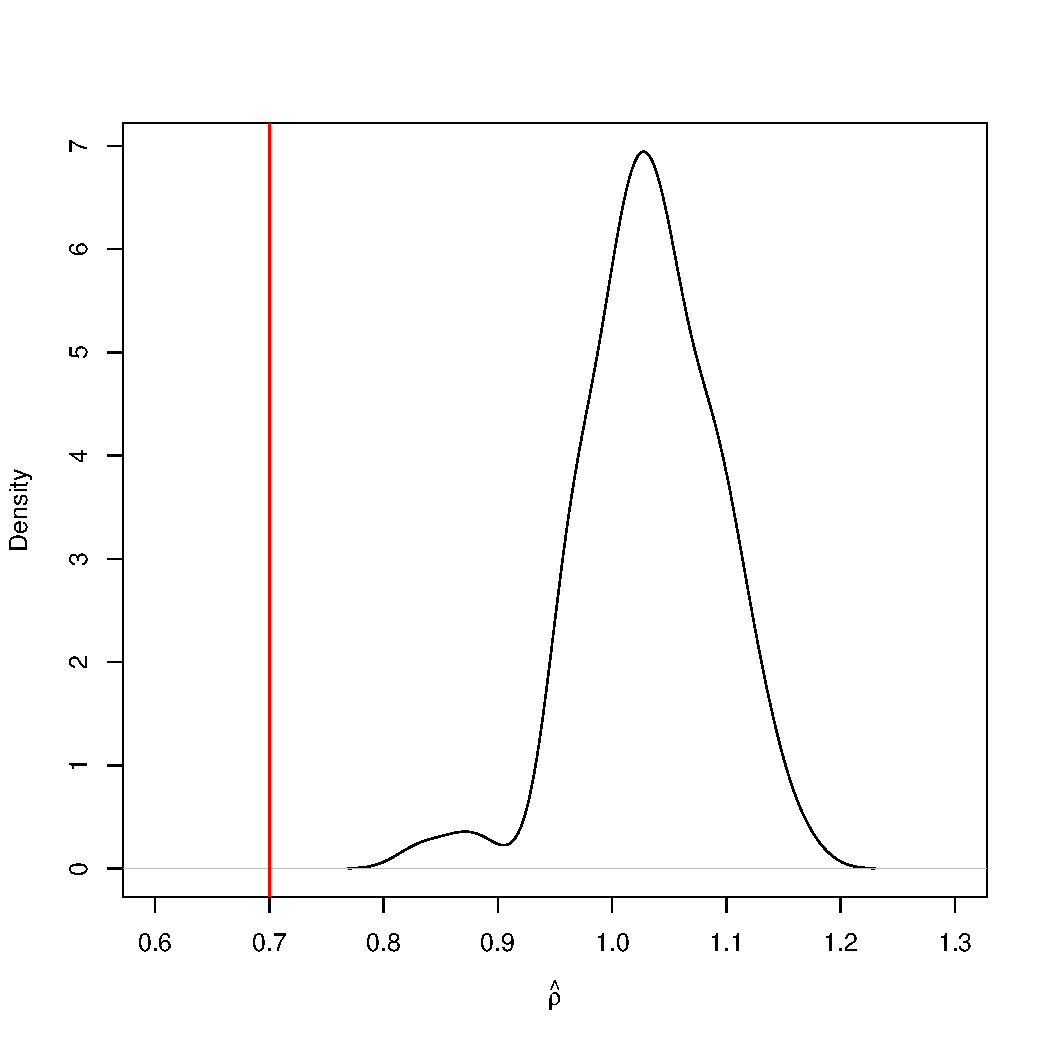
\includegraphics[width=8cm,height=8cm]{figure/ols-rho-sim-1} 

}


\end{knitrout}
\footnotesize
		\emph{Notes:} This graph shows the sampling distribution of $\rho$ estimated by OLS for each sample in the Monte Carlo simulation study. The true DGP follows a pure Spatial Lag Model where the true parameter is $\rho_0 = 0.7$
	\end{minipage}	
\end{figure}

%******************************************************
\section{Maximum Likelihood Estimation of SLM}
%******************************************************

Maximum Likelihood (ML) estimation of spatial lag and spatial error regression models was first derived by \cite{ord1975estimation}. The starting point is the assumption of normality for the error terms. The joint likelihood then follows from the multivariate normal distribution for the dependent variable $\vy$. But unlike the classic OLS, the joint log likelihood for a spatial regression does not equal the sum of the log likelihoods associated with the individual observations. This is due to the spatial simultaneity of the system.

In this Section, we will give further insights about these issues. In particular, we derived the ML estimation procedure for the Spatial Lag Model following very close to \cite{ord1975estimation} and \citet[][chapter 6]{anselin1988spatial}.

%=========================================
\subsection{Maximum Likelihood Function}\index{Maximum likelihood}
%=========================================

The SLM model is given by the following structural model:

\begin{equation}
  \begin{aligned}
    \vy     & = \rho_0 \mW\vy + \mX\vbeta_0 + \vepsi, \\
     \vepsi & \sim \rN(\vzeros_n , \sigma^2_0\mI_n),
  \end{aligned}
\end{equation}
%
where $\vy$ is a vector $n\times 1$ that collects the dependent variable for each spatial unit; $\mW$ is an $n\times n$ spatial weight matrix; $\mX$ is an $n \times k$ matrix of independent variables; $\vbeta_0$ is a known $k$-dimensional vector of parameters; $\rho_0$ measures the degree of spatial correlation; and $\vepsi$ is an $n$-dimensional vector of error terms. Note that we are making the explicit assumption that the error terms follow a multivariate normal distribution with mean $\vzeros$ and variance-covariance matrix $\sigma^2_0\mI_n$. That is, we are assuming that all spatial units have the same error variance. 

Since we are explicitly assuming the distribution of the error term, we will be able to use the maximum likelihood estimation procedure. Under the maximum likelihood criterion, the parameter estimates $\widehat{\vtheta} = (\widehat{\vbeta}^\top, \widehat{\rho}, \widehat{\sigma}^2)^\top$ are chosen so as to maximize the probability of generating or obtaining the observed sample.  However, it should be noted that ML estimation is a highly parametric approach, which means that it is based on strong assumptions. We will see that within these assumptions, it has optimal asymptotic properties (such as consistency and asymptotic efficiency), but when the assumptions are violated, the optimal properties may no longer hold. 

How can we estimate $\vtheta_0$? Note that we can rearrange the model as:

\begin{equation*}
\vy - \rho_0\mW\vy = \mX\vbeta_0 + \vepsi.
\end{equation*}

Following the derivation of the linear model, an estimate for $\vbeta_0$ would be:

\begin{equation*}
\widehat{\vbeta}(\rho_0) = \left(\mX^\top \mX\right)^{-1}\mX^\top\left(\mI_n - \rho_0\mW\right)\vy,
\end{equation*}
%
which depend on $\rho_0$, Given this, an estimate for the variance parameter would be

\begin{equation*}
\widehat{\sigma}^2(\rho_0) = \frac{\widehat{\vepsi}(\rho_0)^\top\widehat{\vepsi}(\rho_0)}{n},
\end{equation*}
%
which also depends on $\rho_0$, and where the residuals $\widehat{\vepsi}(\rho_0)$ will be given by $\widehat{\vepsi}(\rho_0)=\vy - \rho_0\mW\vy - \mX\widehat{\vbeta}$. Since $\widehat{\vbeta}$ and $\widehat{\sigma}^2$ depend on $\rho_0$, we can \emph{concentrate} the full log-likelihood with respect to the parameters $\vbeta, \sigma^2$ and reduce maximum likelihood to an univariate optimization problem in the parameter $\rho$. This will be very useful later in order to derive the ML algorithm.

In order to derive the joint distribution of the data, we need to find the probability density function $f(y_1, y_2,...,y_n| \mX; \vtheta) = f(\vy|\mX;\vtheta)$, that is, the joint conditional distribution of $\vy$ given $\mX$. Using the \textbf{Transformation Theorem}, we know that

\begin{equation*}
  f(\vy | \mX; \vtheta) = f(\vepsi(\vy)| \mX; \vtheta) \left|\frac{\partial \vepsi}{\partial \vy}\right|.
\end{equation*}

Recall that the error term can be written as $\vepsi = \mA\vy - \mX\vbeta$ with $\mA=\mI_n - \rho\mW$ where $\mA\vy$ is \textbf{spatially filtered dependent variable}, i.e., with the effect of spatial autocorrelation taken out. Note that $\vepsi = f(\vy)$, that is, the error vector is a functional form of the observed $\vy$.\footnote{Since $y_i$ and not the $\epsilon_i$ are the observed quantities, the parameters must be estimated by maximizing $L(\vy)$, not $L(\vepsi)$. For more details about this, see \cite{mead1967mathematical} and \cite{doreian1981estimating}.} To move from the the distribution of the error term to the distribution for the observable random variable $\vy$ we need the Jacobian transformation\index{Maximum likelihood!Jacobian}:

\begin{equation*}
\det\left(\frac{\partial \vepsi}{\partial \vy}\right)= \det\left(\mJ\right)=\det(\mA)=\det(\mI_n - \rho\mW),
\end{equation*}
%
where $\mJ = \left(\frac{\partial \vepsi}{\partial \vy}\right)$ is the $n\times n$ Jacobian matrix, and $\det(\mI_n - \rho\mW)$ is the determinant of a $ n \times n$ matrix. In contrast to the time-series case, the spatial Jacobian is not the determinant of a triangular matrix, but of a full matrix. This may complicate its computation considerably. The Jacobian reduces to a scalar 1 in the standard regression model, since the partial derivative becomes $\left|\partial (\vy - \mX\vbeta)/ \partial \vy\right| = \left|\mI_n\right| = 1$. 

Using the density function of the multivariate normal distribution we can find the joint pdf of $\vepsi|\mX$. By recognizing that $\vepsi \sim \rN(\vzeros, \sigma^2\mI_n)$, we can write: 

\begin{equation*}
	f(\vepsi | \mX) = (2\pi \cdot\sigma^2)^{-n/2}\exp\left[-\frac{1}{2\sigma^2}\vepsi^\top\vepsi\right].
\end{equation*}

Given an i.i.d sample of $n$ observations, $\vy$ and $\mX$, the joint density of the observed sample is:

\begin{equation*}
	f(\vy|\mX;\vtheta) = (2\pi \cdot\sigma^2)^{-n/2}\exp\left[-\frac{1}{2\sigma^2}(\mA\vy-\mX\vbeta)^\top (\mA\vy-\mX\vbeta)\right]\det\left(\frac{\partial (\mA\vy - \mX\vbeta)}{\partial \vy}\right).
	\end{equation*}
	
Note that the likelihood function is defined as the joint density treated as a function of the parameters: $L(\vtheta|\vy, \mX) = f(\vy|\mX;\vtheta)$. Finally, the log-likelihood function, which will be maximized, takes the form:\footnote{Since the constant $- \frac{n\log(2\pi)}{2}$ is not a function of any of the parameters, some software programs do not include it when reporting maximized log-likelihood. See \cite{spdep}.}

\begin{equation} \label{eq:LL_SLM_2}
  \begin{aligned}
\log L(\vtheta) &= \log\left| \mA\right| - \frac{n\log(2\pi)}{2} - \frac{n\log(\sigma^2)}{2} - \frac{1}{2\sigma^2}(\mA\vy-\mX\vbeta)^\top (\mA\vy-\mX\vbeta) \\
&= \log\left| \mA\right| - \frac{n\log(2\pi)}{2} - \frac{n\log(\sigma^2)}{2} - \frac{1}{2\sigma^2}\left[\vy^\top \mA^\top\mA\vy - 2\left(\mA\vy\right)^\top\mX\vbeta + \vbeta^\top\mX^\top\mX\vbeta\right],
\end{aligned}
\end{equation}	
%	
where this development uses the fact that the transpose of a scalar is the scalar, i.e., 	$\vy^\top\mA^\top\mX\vbeta = (\vy^\top\mA\mX\vbeta)^\top = \vbeta^\top\mX^\top\mA\vy$. This is similar to the typical linear-normal likelihood, except that the transformation from $\vepsi$ to $\vy$, is not by the usual factor of 1, but by $\log\left| \mA\right|$.

As we will show in Section XX, we can directly estimate the $\vtheta$ by maximizing the log-likelihood function \eqref{eq:LL_SLM_2} using a constrained optimization algorithm. However, as shown in the next Section, we can create a more easy estimation algorithm by concentrating the log-likelihood function. 

%=========================================
\subsection{Score Vector and Estimates}\label{sec:score_sml}
%=========================================

In order to find the ML estimates for the SLM model, we need to maximize Equation (\ref{eq:LL_SLM_2}) with respect to $\vtheta = (\vbeta^\top, \sigma^2 , \rho)^\top$. To do so, we need to find the first order condition (FOC) of this optimization problem. 

Before taking derivatives it is useful to review some important properties of matrix calculus given in the next definition. 

\begin{definition}[Some useful results on matrix calculus]\label{definition:matrix_cal_sar}
Some important results  are the followings:

\begin{equation}\label{eq:mc_1}
\frac{\partial (\rho \mW)}{\partial \rho} = \mW
\end{equation}

\begin{equation}\label{eq:mc_2}
  \begin{aligned}
\frac{\partial \mA}{\partial \rho} & = \frac{\partial (\mI_n - \rho\mW)}{\partial \rho} \\
                                   & = \frac{\partial \mI_n}{\partial \rho} - \frac{\partial \rho\mW}{\rho} \\
                                   & = -\mW
 \end{aligned}
\end{equation}

\begin{equation}\label{eq:mc_3}
\frac{\partial \log \left|\mA\right|}{\partial \rho}  = \tr(\mA^{-1}\partial \mA / \partial \rho) = \tr\left[\mA^{-1}(-\mW)\right]
\end{equation}

Let $\vepsi = \mA\vy - \mX\vbeta$, then:

\begin{equation}\label{eq:mc_4}
  \frac{\partial \vepsi}{\partial \rho} =  \frac{\partial (\mA\vy - \mX\vbeta)}{\partial \rho} = -\mW\vy 
\end{equation}

\begin{equation}\label{eq:mc_5}
  \frac{\partial \vepsi^\top \vepsi}{\partial \rho} = \vepsi^\top (\partial \vepsi / \partial \rho) + (\partial \vepsi ^\top / \partial \rho)\vepsi = 2\vepsi^\top (\partial \vepsi / \partial \rho) = 2\vepsi^\top(-\mW)\vy
\end{equation}

\begin{equation}\label{eq:mc_6}
  \frac{\partial \mA^{-1}}{\partial \rho} = -\mA^{-1}(\partial \mA / \partial \rho)\mA^{-1} = \mA^{-1} \mW \mA^{-1}
\end{equation}

\begin{equation}\label{eq:mc_7}
  \frac{\partial \tr\left(\mA^{-1} \mW\right)}{\partial \rho} = \tr\left(\partial \mA^{-1}\mW / \partial \rho\right) 
\end{equation}
\end{definition}

Taking the derivative of Equation (\ref{eq:LL_SLM_2}) respect to $\vbeta$, we obtain:

\begin{equation}\label{eq:foc_ml_sar_beta}
\frac{\partial \log L(\vtheta)}{\partial \vbeta} = -\frac{1}{2\sigma^2}\left[-2\left(\left(\mA\vy\right)^\top\mX\right)^\top + 2 \mX^\top\mX\vbeta\right] = \frac{1}{\sigma^2}\mX^\top(\mA\vy - \mX\vbeta),
\end{equation}
%
and with respect to $\sigma^2$ yields:

\begin{equation}\label{eq:foc_ml_sar_sigma}
\frac{\partial \log L(\vtheta)}{\partial \sigma^2} = -\frac{n}{2\sigma^2} + \frac{1}{2\sigma^4}\left(\mA\vy - \mX\vbeta\right)^\top\left(\mA\vy - \mX\vbeta\right).
\end{equation}

Setting both (\ref{eq:foc_ml_sar_beta}) and (\ref{eq:foc_ml_sar_sigma}) to 0 and solving, we obtain:

\begin{eqnarray}
	\widehat{\vbeta}_{ML}(\rho) &=& \left(\mX^\top\mX\right)^{-1}\mX^\top\mA\vy \label{eq:beta_ML} \\
	\widehat{\sigma}^2_{ML}(\rho) &=& \frac{\left(\mA\vy - \mX\vbeta_{ML}\right)^\top\left(\mA\vy - \mX\vbeta_{ML}\right)}{n}\label{eq:sigma_ML}.
\end{eqnarray}

Note that conditional on $\rho$ (assuming we know $\rho$), these estimates are simply OLS applied to the \emph{spatial filtered} dependent variable $\mA\vy$ and the exploratory variables $\mX$. Moreover, after some manipulation, Equation (\ref{eq:beta_ML}) can be re-written as:

\begin{eqnarray}\label{eq:beta_Ml_2}
\vbeta_{ML}(\rho) &=& \left(\mX^\top\mX\right)^{-1}\mX^\top\vy - \rho\left(\mX^\top\mX\right)^{-1}\mX^\top\mW\vy \nonumber \\
&=& \widehat{\vbeta}_O -\rho \widehat{\vbeta}_L\label{eq:beta_ml_exp}.
\end{eqnarray}

Note that the first term in  (\ref{eq:beta_Ml_2}) is just the OLS regression of $\vy$ on $\mX$, whereas the second term is just $\rho$ times the OLS regression of $\mW\vy$ on $\mX$. Next, define the following:

\begin{equation}\label{eq:SLM_aux_residuals}
\ve_O = \vy - \mX\widehat{\vbeta}_0\,\,\mbox{and} \;\; \ve_L = \mW\vy - \mX\widehat{\vbeta_L}.
\end{equation}

Then, plugging (\ref{eq:beta_ml_exp}) into (\ref{eq:sigma_ML})

\begin{eqnarray}\label{eq:sigma_ml_con}
\sigma^2_{ML}\left[\vbeta_{ML}(\rho) , \rho\right] &=& \frac{\left(\ve_O - \rho\ve_L\right)^\top\left(\ve_O - \rho\ve_L\right)}{n}.
\end{eqnarray}

Note that both (\ref{eq:beta_ml_exp}) and (\ref{eq:sigma_ml_con}) rely only on observables, except for $\rho$, and so are readily calculable given some estimate of $\rho$. Therefore, plugging (\ref{eq:beta_ml_exp}) and (\ref{eq:sigma_ml_con}) back into the likelihood (\ref{eq:LL_SLM_2})  we obtain the \textbf{concentrated log-likelihood function}\index{Maximum likelihood!concentrated log-likelihood}:

\begin{equation}\label{eq:concentrated_ml_sar_1}
\log L(\rho)_c=-\frac{n}{2}-\frac{n}{2}\log(2\pi) - \frac{n}{2}\log\left[\frac{\left(\ve_O - \rho\ve_L\right)^\top\left(\ve_O - \rho\ve_L\right)}{n}\right] + \log\left|\mI_n - \rho\mW\right|,
\end{equation}	
%	
which is a \textbf{nonlinear} function of a single parameter $\rho$. A ML estimate for $\rho$, $\widehat{\rho}_{ML}$, is obtained from a numerical optimization of the concentrated log-likelihood function (\ref{eq:concentrated_ml_sar_1}). Once we obtain $\widehat{\rho}$, we can easily obtain $\widehat{\vbeta}$.  The procedure can be summarized in the following steps:

\begin{algorithm}[ML estimation of SLM]\label{algorithm:SLM}
The algorithm to perform the ML estimation of the SLM is the following: 
\begin{enumerate}
	\item Perform the two auxiliary regression of $\vy$ and $\mW\vy$ on $\mX$ to obtain $\widehat{\vbeta}_O$ and $\widehat{\vbeta}_L$ as in Equation (\ref{eq:beta_Ml_2}).
	\item Use $\widehat{\vbeta}_O$ and $\widehat{\vbeta}_L$ to compute the residuals in Equation (\ref{eq:SLM_aux_residuals}). 
	\item Maximize the concentrated likelihood given in Equation (\ref{eq:concentrated_ml_sar_1}) by numerical optimization to obtain an estimate of $\rho$.
	\item Use the estimate of $\widehat{\rho}$ to plug it back in to the expression for $\vbeta$ (Equation \ref{eq:beta_ML}) and $\sigma^2$	 (Equation \ref{eq:sigma_ML}).
\end{enumerate}	
\end{algorithm}

Since the score function will be important for understanding the asymptotic theory of MLE, we will derive also $\partial \log L(\vtheta) / \partial \rho$. Taking the derivative of Equation (\ref{eq:LL_SLM_2}) respect to $\rho$, we obtain:

\begin{equation}\label{eq:der1_rho}
  \begin{aligned}
      \frac{\partial \log L(\vtheta)}{\partial \rho} & =  \left(\frac{\partial}{\partial \rho}\right)\log \left| \mA\right| -  \frac{1}{2\sigma^2}\left(\frac{\partial}{\partial \rho}\right)\vepsi^\top \vepsi \\
      & = - \tr(\mA^{-1}\mW) +\frac{1}{2\sigma^2}2\vepsi^\top\mW\vy\quad\mbox{Using (\ref{eq:mc_3}) and (\ref{eq:mc_5})} \\
      & = - \tr(\mA^{-1}\mW) +\frac{1}{2\sigma^2}2\vepsi^\top\mW\vy \\
      & = - \tr(\mA^{-1}\mW) +\frac{1}{\sigma^2}\vepsi^\top\mW\vy. 
  \end{aligned}
\end{equation}

Thus the complete gradient (or score function) is:

\begin{equation}\label{eq:full_agradient}
  \nabla_{\vtheta} = \frac{\partial \log L(\vtheta)}{\partial \vtheta} = 
    \begin{pmatrix}
    \frac{\partial \log L(\vtheta)}{\partial \vbeta} \\
    \frac{\partial \log L(\vtheta)}{\partial \sigma^2} \\
    \frac{\partial \log L(\vtheta)}{\partial \rho}
    \end{pmatrix}
    =
    \begin{pmatrix}
    \frac{1}{\sigma^2}\mX^\top\vepsi \\
    \frac{1}{2\sigma^4}(\vepsi^\top\vepsi-n\sigma^2) \\
    - \tr(\mA^{-1}\mW) +\frac{1}{\sigma^2}\vepsi^\top\mW\vy
    \end{pmatrix}
\end{equation}

Note that if we replace $\vy = \mA^{-1}\mX\vbeta + \mA^{-1}\vepsi$ in Equation (\ref{eq:der1_rho}), we get:

\begin{equation*}
 \frac{\partial \log L(\vtheta)}{\partial \rho} = \frac{1}{\sigma^2}(\mC\mX\vbeta)^\top \vepsi + \frac{1}{\sigma^2}(\vepsi^\top\mC\vepsi - \sigma^2 \tr(\mC)),
\end{equation*}
%
where:

\begin{equation}\label{eq:Cmatrix}
  \mC = \mW\mA^{-1}.
\end{equation}

%**********************
\subsection{Hessian}
%***********************

The Hessian matrix will be very important in the following sections to obtain the asymptotic variance-covariance matrix. For this reason we devote a complete section in order to derive this matrix for the SLM. In this case, the Hessian is a $(k + 2)\times (k + 2)$ matrix of second derivatives given by :

\begin{equation*}
	\mH(\vbeta, \sigma^2, \rho) = 
	\begin{pmatrix}
		\frac{\ell(\vbeta, \sigma^2,\rho)}{\partial \vbeta \partial \vbeta^\top} & \frac{\ell(\vbeta, \sigma^2,\rho)}{\partial \vbeta \partial \sigma^2} & \frac{\ell(\vbeta, \sigma^2,\rho)}{\partial \vbeta \partial \rho} \\
		\frac{\ell(\vbeta, \sigma^2,\rho)}{\partial \sigma^2 \partial \vbeta^\top} & \frac{\ell(\vbeta, \sigma^2,\rho)}{\partial (\sigma^2)^2} & \frac{\ell(\vbeta, \sigma^2,\rho)}{\partial \sigma^2 \partial \rho} \\
		\frac{\ell(\vbeta, \sigma^2,\rho)}{\partial \rho \partial \vbeta^\top} & \frac{\ell(\vbeta, \sigma^2,\rho)}{\partial \rho \partial \sigma^2} & \frac{\ell(\vbeta, \sigma^2,\rho)}{\partial \rho^2}
	\end{pmatrix} 
\end{equation*}

Now we work in the cross-derivatives for $\vbeta$. From (\ref{eq:foc_ml_sar_beta}):

\begin{align}
  \frac{\partial^2 \log L(\vtheta)}{\partial \vbeta \partial \vbeta^\top}  & =  - \frac{1}{\sigma^2}(\mX^\top \mX) \label{eq:sar_der_beta_beta} \\
  \frac{\partial^2  \log L(\vtheta)}{\partial \vbeta \partial \sigma^2} &= - \frac{1}{(\sigma^2)^2} \mX^\top \vepsi\label{eq:sar_der_beta_sigma} \\
  \frac{\partial^2  \log L(\vtheta)}{\partial \vbeta \partial \rho}  & =  - \frac{1}{\sigma^2} \mX^\top \mW\vy\label{eq:sar_der_beta_rho},
\end{align}


Using the first derivative (\ref{eq:foc_ml_sar_sigma}) and working in the cross-derivatives for $\sigma^2$, we obtain:

\begin{equation}\label{eq:sar_der_sigma_sigma}
	\frac{\partial^2 \log L(\vtheta)}{\partial (\sigma^2)^2}  = \frac{n}{2(\sigma^2) ^2} - \frac{1}{(\sigma^2)^3} \vepsi^\top \vepsi
\end{equation}
%
and:

\begin{equation}\label{eq:sar_der_sigma_rho}
\begin{aligned}
\frac{\partial \log L(\vtheta) }{\partial \sigma^2 \partial \rho}  & = \frac{1}{2\sigma ^ 4}\left[2\vepsi^\top \left(\frac{\partial \vepsi}{\partial \rho}\right)\right] \quad \mbox{Using Equation (\ref{eq:mc_5})}\\
& =  - \frac{1}{\sigma ^ 4}\vepsi ^\top \mW\vy \\
& =  -\frac{\vepsi^\top\mW\vy}{\sigma ^ 4}
\end{aligned}
\end{equation}

Finally, working in the second derivative of $\rho$, and using (\ref{eq:der1_rho}), we obtain

\begin{equation}\label{eq:sar_der_rho_rho}
\begin{aligned}
\frac{\partial \log L(\vtheta) }{\partial \rho ^2}  & = -\left(\frac{\partial }{\partial \rho}\right)\tr(\mA^{-1}\mW) + \frac{1}{\sigma^2}\left(\frac{\partial }{\partial \rho}\right)\vepsi^\top\mW\vy \\
& = - \tr\left( \frac{\partial \mA^{-1}\mW}{\partial \rho}\right) + \frac{1}{\sigma^2}\left(\frac{\partial }{\partial \rho}\right)(\mA\vy)^\top\mW\vy \\
& = - \tr\left( \mA^{-1}\mW\mA^{-1}\mW \right)+ \frac{1}{\sigma^2}(- \vy^{\top}\mW^{\top}\mW\vy) \\
& = - \tr\left[(\mW\mA^{-1})^2\right] - \frac{1}{\sigma^2}(\vy^{\top}\mW^{\top}\mW\vy)
\end{aligned}
\end{equation}


Therefore, the Hessian is:

\begin{equation}\label{eq:hessian_sml}
	\mH(\vbeta, \sigma^2, \rho) = 
	\begin{pmatrix}
	- \frac{1}{\sigma^2}(\mX^\top \mX) & - \frac{1}{(\sigma^2)^2} \mX^\top \vepsi & - \frac{1}{\sigma^2} \mX^\top \mW\vy \\
		 .& \frac{n}{2(\sigma^2) ^2} - \frac{1}{(\sigma^2)^3} \vepsi^\top \vepsi & -\frac{\vepsi^\top\mW\vy}{\sigma ^ 4} \\
		 .& . & - \tr\left[(\mW\mA^{-1})^2\right] - \frac{1}{\sigma^2}(\vy^{\top}\mW^{\top}\mW\vy)
	\end{pmatrix} 
\end{equation}
%
which is symmetric and $\mC$ is given in Equation \eqref{eq:Cmatrix}.

%=============================
\subsection{Ord's Jacobian}
%=============================

An important feature of the concentrated log-likelihood function (\ref{eq:concentrated_ml_sar_1}) is the Jacobian term $\left|\mI_n - \rho\mW\right|$. Computationally this is burdensome, since determining $\widehat{\rho}$ rests on the evaluation of the $n\times n$ matrix $\left|\mI_n - \rho\mW\right|$ in each iteration. However, \cite{ord1975estimation} note that:

\begin{equation*}
	\left|\omega\mI_n -\mW\right|=\prod_{i=1}^n(\omega-\omega_i).
\end{equation*}	

Therefore:

\begin{equation*}
\left|\mI_n -\rho\mW\right|=\prod_{i=1}^n(1-\rho\omega_i),
\end{equation*}	
%
and the log-determinant term follows as

\begin{equation}\label{eq:Ord-determinant}
\log\left|\mI_n -\rho\mW\right|=\sum_{i=1}^n\log(1 - \rho\omega_i).
\end{equation}

The advantage of this approach is that the eigenvalues only need to be computed once, which carries some overhead, but greatly speeds up the calculation of the log-likelihood at each iteration. In practice, in all but the smallest data sets (< 4000 observations), the Ord's approach will be faster than the brute force approach. 

This new formulation give us the possible domain of $\rho$. We need that $1 - \rho \omega_i \neq 0$, which occurs only if $1/\omega_{min} < \rho < 1/\omega_{max}$. For row-standardized matrix, the largest eigenvalues is 1. With this new approximation,  the new concentrated log-likelihood function is:

\begin{equation}\label{eq:concentrated_ml_sar_2}
  \begin{aligned}
\log L(\rho)_c & =-\frac{n}{2}-\frac{n}{2}\log(2\pi) - \frac{n}{2}\log\left[\frac{\left(\ve_O - \rho\ve_L\right)^\top\left(\ve_O - \rho\ve_L\right)}{n}\right] + \sum_{i=1}^n\log(1 - \rho\omega_i), \\
& = \mbox{const}- \log\left[\frac{\ve_O^\top\ve_O - 2\rho\ve_L^\top\ve_O + \rho^2 \ve_L^\top\ve_L}{n}\right] + \frac{2}{n}\sum_{i=1}^n\log(1 - \rho\omega_i).
  \end{aligned}
\end{equation}	

Another method approach is the characteristic root method outlined in \cite{smirnov2001fast}. This approach allows for the estimation of spatial lag models for very large data sets (> 100,000 observations) in a very short time. However, it is limited by the requirement that the weight matrix needs to be intrinsically symmetric. This precludes the use of asymmetric weight such as $k$-nearest neighbor weights. For other approximations see \citet[][chapter 4]{lesage2010introduction}.

%**************************************
\section{Maximum Likelihood Estimation of SEM}\label{sec:sem-ml}
%*************************************

\subsection{What Are The Consequences of Applying OLS on a SEM Model?}

As we reviewed in Section \ref{sec:tax_SEM}, a second way to incorporate spatial autocorrelation in a regression model is to specify a spatial process for the error term.  The SEM model is given by

\begin{equation}\label{eq:sem_ml}
	\begin{aligned}
	\vy  & = \mX\vbeta_0 + \vu \\ 
	 \vu & = \lambda_0 \mW \vu + \vepsi \\
	 \vepsi & \sim \rN(\vzeros, \sigma^2_0\mI_n)
	\end{aligned}
\end{equation}
%
where $\lambda_0$ is the spatial autoregressive coefficient for the error lag $\mW\vu$ (to distinguish the notation from the spatial autoregressive coefficient $\rho$ in a spatial lag model), $\mW$ is the spatial weight matrix, $\vepsi$ is an error $\vepsi \sim N(\vzeros, \sigma^2_0\mI_n)$. This model do not require a theoretical model for a spatial process, but instead, is consistent with a situation where determinants of the dependent variable omitted from the model are \textbf{spatially autocorrelated}, or with a situation where unobserved shocks follows a spatial pattern \citep{elhorst2014spatial}. In summary, SEM treats spatial correlation primarily as a nuisance. 

If $\lambda > 0$, then we face positive spatial correlation. This implies clustering of similar values; that is, the errors for spatial unit $i$ tend to vary systematically with the errors for other nearby observations $j$ so that smaller/larger errors for $i$ would tend to go together with smaller/larger errors for $j$. This violates the typical assumption of no autocorrelation in the error term of the OLS. 

Under the assumption that the spatial weights matrix is row standardized and the parameter is less than one in absolute value, the model can be also be expressed as:

\begin{equation*}
	\vy = \mX\vbeta + \left(\mI_n-\lambda\mW\right)^{-1}\vepsi.
\end{equation*}

Since $\vu = (\mI_n - \lambda\mW)^{-1}\vepsi$, it can be shown that $\E(\vu| \mW, \mX) = \vzeros$. Furthermore, the variance-covariance matrix of $\vu$ is: 

\begin{equation}\label{eq:cov_error_sem}
\var(\vu| \mW, \mX)=\E(\vu\vu^\top| \mW, \mX) = \sigma^2(\mI_n-\lambda\mW)^{-1}(\mI-\lambda\mW^\top)^{-1}=\sigma^2\mOmega_{u}^{-1},
\end{equation}
%
where $\mOmega_{u}=(\mI_n-\lambda\mW)(\mI_n-\lambda\mW)^\top$. The variance covariance (\ref{eq:cov_error_sem}) is a full matrix implying a spatial autoregressive error process leading to a nonzero error covariance between every pair of observations, but decreasing in magnitude with the order of contiguity \citep{AnselinBera1998}. Furthermore, the complex structure in the inverse matrix in (\ref{eq:cov_error_sem}) yields nonconstant diagonal elements in the error covariance matrix, thus inducing heteroskedasticity in $\vu$, irrespective of the heteroskedasticity of $\vepsi$. Finally, $\vu \sim \rN(\vzeros, \sigma^2\mOmega_u^{-1})$.


\begin{remark}\label{remark:ols_sem}
  The OLS estimates of model in Equation (\ref{eq:sem_ml}) are unbiased, but inefficient if $\lambda \neq 0$.
\end{remark}

Given the previous Remark, we might used generalized least squares (GLS) for a more efficient parameters estimation. Recall that the inefficiency of OLS estimates of the regression coefficient would invalidate the statistical inference in the spatial error model. The invalidity of significance test arises from biased estimation of the variance and standard errors of the OLS estimates for $\vbeta$ and $\lambda$.

%----------------------------------------
\subsection{Log-likelihood function}
%----------------------------------------

The model in Equation (\ref{eq:sem_ml}) implies that the reduced form is :

\begin{equation*}
\vepsi = \left(\mI-\lambda\mW\right)\vy - \left(\mI_n-\lambda\mW\right)\mX\vbeta = \mB\vy - \mB\mX\vbeta,
\end{equation*}
%
where $\mB = (\mI_n-\lambda\mW)$. Recall that in order to create the log-likelihood function we need the joint density function. Using the Transformation Theorem we are able to find the joint conditional function:

\begin{equation*}
  f(y_1,...,y_n|\mX; \vtheta) = f(\vepsi(\vy)| \mX ; \vtheta) \cdot \left|\mJ\right|.
\end{equation*}

Again, the Jacobian term is not equal to one, but instead is

\begin{equation*}
\mJ = \frac{\partial \vepsi}{\partial \vy} =\mB.
\end{equation*}

Thus, the joint density function of $\vepsi$---which is a function of $\vy$--- equals

\begin{equation*}
  f(\vepsi(\vy)| \mX ; \vtheta) = (2\pi \sigma^2)^{-n/2}\exp\left[- \frac{\left[\left(\mI_n-\lambda\mW\right)(\vy - \mX\vbeta)\right]^\top \left[\left(\mI_n-\lambda\mW\right)(\vy - \mX\vbeta)\right]}{2\sigma^2}\right],
\end{equation*}
%
and the joint density function of $\vy$, $f(y_1,...,y_n|\mX; \vtheta)$ equals

\begin{equation*}
  f(\vy| \mX ; \vtheta) = (2\pi \sigma^2)^{-n/2}\exp\left[- \frac{(\vy - \mX\vbeta)^\top \mB^\top \mB (\vy - \mX\vbeta)}{2\sigma^2}\right]\cdot \left|\mB\right|
\end{equation*}

Finally, the log-likelihood can be expressed as

\begin{equation}\label{eq:ll_sem}
\log L(\vtheta) = - \frac{n}{2}\log(2\pi) - \frac{n}{2}\log(\sigma^2)-\frac{(\vy - \mX\vbeta)^\top \mOmega(\lambda) (\vy - \mX\vbeta)}{2\sigma^2} + \log\left|\mI_n - \lambda \mW\right|,
\end{equation}
%
where 

\begin{equation*}
\mOmega(\lambda) = \mB^\top \mB = \left(\mI_n-\lambda\mW\right)^\top \left(\mI_n-\lambda\mW\right)
\end{equation*}


Again, we run into complications over the log of the determinant $\left|\mI_n - \lambda \mW\right|$, which is an $n$th-order polynomial that is cumbersome to evaluate. 

\subsection{Score Function and ML Estimates}\label{sec:sem_ml_estimates}

Maximizing the log-likelihood function (\ref{eq:ll_sem}) is the same as to minimizing the sum of the transformed errors, $\vepsi^\top\vepsi$, corrected by the log of the Jacobian, $\log\left|\mI_n - \lambda \mW\right|$. Since we are accounting for this correction, the ML estimates will differ from the OLS estimates. They will coincide if $\lambda \to 0$. 

To obtain the ML estimates, we apply FOC to the log-likelihood function (\ref{eq:ll_sem}). Taking the derivative respect to $\vbeta$ yields:

\begin{equation}\label{eq:beta_gls_ml}
  \begin{aligned}
\vbeta_{ML}(\lambda) & =\left[\mX^\top\mOmega(\lambda)\mX\right]^{-1}\mX^\top\mOmega(\lambda)\vy\\
                     & = \left[(\mB\mX)^\top (\mB \mX)\right]^{-1} (\mB\mX)^\top \mB \vy \\
                     & = \left[\mX(\lambda)^\top  \mX(\lambda)\right]^{-1} \mX(\lambda)^\top \vy(\lambda),
  \end{aligned}
\end{equation}
%
where:

\begin{equation}
  \begin{aligned}
\mX(\lambda) & = \mB\mX = (\mI - \lambda\mW)\mX = (\mX - \lambda\mW\mX) \\
\vy(\lambda) & = (\vy - \lambda \mW \vy).
  \end{aligned}
\end{equation}

If $\lambda$ is known, this estimator is equal to the GLS estimator---$\widehat{\beta}_{ML} = \widehat{\beta}_{GLS}$---and it can be thought as the OLS estimator resulting from a regression of $\vy(\lambda)$ on $\mX(\lambda)$. In other words, for a known value of the spatial autoregressive coefficient ,$\lambda$, this is equivalent to OLS on the transformed variables.


\begin{remark}
In the literature, the transformations:

\begin{eqnarray*}
\mX(\lambda) &=&(\mX - \lambda\mW\mX) \\
\vy(\lambda) &=& (\vy - \lambda \mW \vy)
\end{eqnarray*}

are known as the \emph{Cochrane-Orcutt transformation}.
\end{remark}

In the same way, a first-order condition resulting from the spatial derivative of (\ref{eq:ll_sem}) with respect to $\sigma^2$ gives the ML estimator for the error variance:

\begin{equation}
	\sigma^2_{ML}(\lambda) = \frac{1}{n}\left(\widehat{\vepsi}^\top\mB^\top\mB \vepsi\right)= \frac{1}{n}\widehat{\vepsi}^\top(\lambda)\widehat{\vepsi}(\lambda)
\end{equation}
%
where $\widehat{\vepsi} = \vy - \mX\widehat{\vbeta}_{ML}$ and $\widehat{\vepsi}(\lambda) = \mB(\lambda)(\vy - \mX\widehat{\vbeta}_{ML}) = \mB(\lambda)\vy - \mB(\lambda)\mX\widehat{\vbeta}_{ML}$. 


First order condition derived from the expression of the likelihood are highly non-linear and therefore the likelihood in Equation (\ref{eq:ll_sem}) cannot be directly maximized. Again, a concentrated likelihood approach is necessary.

The estimators for $\vbeta$ and $\sigma^2$ are both functions of the value of $\lambda$. A concentrated log-likelihood can then be obtained as:


\begin{equation}
	\log L(\lambda)^c= \mbox{const} + \frac{n}{2}\log\left[\frac{1}{n}\widehat{\vepsi}^\top\mB^\top\mB \widehat{\vepsi}\right] + \log\left|\mB\right|
\end{equation}

The residual vector of the concentrated likelihood is also, indirectly, a function of the spatial autoregressive parameter.

A one-time optimization will in general not be sufficient to obtain maximum likelihood estimates for all the parameters. Therefore an interactive procedure will be needed.

Alternate back and forth between the estimation of the spatial autoregressive coefficient conditional upon residuals (for a value of $\vbeta$), and a estimation of the parameter vector (conditional upon the s.a.c). 

\begin{algorithm}[ML estimation of SEM]

Following \cite{anselin1988spatial}, the procedure can be summarize in the following steps:

\begin{enumerate}
		\item Carry out an OLS of $\mB\mX$ on $\mB\vy$; get $\widehat{\vbeta}_{OLS}$
		\item Compute initial set of residuals $\widehat{\epsilon}_{OLS} = \mB\vy - \mB\mX\widehat{\vbeta}_{OLS}$
		\item Given $\widehat{\epsilon}_{OLS} $, find $\widehat{\lambda}$ that maximizes the concentrated likelihood.
		\item If the convergence criterion is met, proceed, otherwise repeat steps 1, 2 and 3.
		\item Given $\widehat{\lambda}$, estimate $\widehat{\vbeta}(\lambda)$ by GLS and obtain a new vector of residuals, $\widehat{\vepsi}(\lambda)$
		\item Given  $\widehat{\vepsi}(\lambda)$ and $\widehat{\lambda}$, estimate $\widehat{\sigma}(\lambda)$.
\end{enumerate}	
\end{algorithm}


Finally, the asymptotic variance-covariance matrix is:

\begin{equation}\label{eq:asyvar_sem}
\mbox{AsyVar}(\vbeta, \sigma^2, \lambda)  = 
\begin{pmatrix}
 \underset{k \times k}{\frac{\mX(\lambda)\top\mX(\lambda)}{\sigma^2}} & 0 & 0 \\
  0 & \frac{n}{2\sigma^4} & \frac{\tr(\mW_B)}{\sigma^2} \\
 0 & \frac{\tr(\mW_B)}{\sigma^2} & \tr(\mW_B)^2 + \tr(\mW_B^\top\mW_B)
\end{pmatrix}^{-1}
\end{equation}
%
where $\mW_B = \mW(\mI - \lambda\mW)^{-1}$.

%====================================
\section{Asymptotic Properties}
%====================================


In this section we review the asymptotic properties of the ML and Quasi ML for the SLM. In particular, we follow \cite{lee2004asymptotic}.

%------------------------------------
\subsection{Consistency of QMLE}
%------------------------------------


\cite{lee2004asymptotic} derives the asymptotic properties (consistency and asymptotic normality) of the ML and QML estimator for the SLM model. \cite{lee2004asymptotic} starts with the following assumption about the error terms $\epsilon_{i}$. 

\begin{assumption}[Errors]\label{assu:ml_1}
Assume the following
  \begin{enumerate}
    \item The disturbances $\left\lbrace \epsilon_{i,n}: 1 \leq i \leq n, n\geq 1\right\rbrace$ are identically distributed. Furthermore, for each sample size $n$, they are jointly independent distributed with mean $ \E(\epsilon_{i, n}) = 0$ and $\E(\epsilon_{i, n}^2)=\sigma^2_{\epsilon, n}$ where $0 < \sigma^2_{\epsilon, n} < b$. 
    \item Its moments $\E\left(|\epsilon_{i,n}|^{4 + \gamma}\right)$ for some $\gamma > 0$ exits.
  \end{enumerate}  
\end{assumption}

Note that Assumption \ref{assu:ml_1}(1) allows the error term to depend on the sample size $n$, i.e., to form a triangular array. %(For simplicity of notation we will, for the most part, drop again subscripts $n$ in the following).

Moreover, because statistics involving quadratic forms of $\epsilon_n$ will be present in the estimation, the existence of the fourth order moment of $\epsilon_{i,n}$ will guarantee finite variances for the quadratic forms and we will be able to apply a CLT. 

In order to understand the asymptotic behavior of $\mW_n$ under some \textbf{regularity conditions}, we need to understand some useful terminologies.

\begin{definition}[Triangular array of constants]\label{def:tria_array_const}
Let $\left\lbrace b_{ni} \right\rbrace, i = 1,...,n$ be a triangular array of constants.

\begin{enumerate}
  \item $\left\lbrace b_{ni} \right\rbrace$ are at most of order $(1/h_n)$, denoted by $O(1/h_n)$ uniformly in $i$ if there exists a finite constant $c$ independent of $i$ and $n$ such that $\left|b_{ni}\right|\leq \frac{c}{h_n}$ for all $i$ and $n$.
  \item $\left\lbrace b_{ni} \right\rbrace$ are bounded away from zero uniformly in $i$ at rate of $h_n$ if there exists a positive sequence $\left\lbrace h_{n} \right\rbrace$ and a constant $c>0$ independent of $i$ and $n$ such that $c\leq \left|b_{ni}\right|/ h_n$ for all $i$ for sufficiently large $n$.
\end{enumerate}
\end{definition}

Again, we must think the $\mW$ matrices as triangular arrays of constants. Recall that the elements of $\mW$ are denoted as $w_{ij}$.  However, since as we add more spatial units the spatial structure changes, it might be the case that the element $w_{ij}$ is not the same when $n = 50$ or $n = 55$. Therefore, we need triangular arrays in order to make explicit this possibility. That is why we will index the elements of $\mW_n$ as $w_{n, ij}$.

Another question is whether each element of $\mW_n$---or sequences--- are bounded. That is, they are limited as $n\to \infty$. In this context, Definition \ref{def:tria_array_const} provides a specific setting for sequences bounded away from zero. If sequences are divergent, this definition describes how fast the sequences tend to infinity. Now, we apply this definition to the spatial weight matrices:

\begin{assumption}[Weight Matrix]\label{assu:ml_2}
	The elements $w_{n,ij}$ of $\mW_n$ are at most of order $h_n^{-1}$, denoted by $O(1/h_n)$, uniformly in all $i,j$, where the rate sequence ${h_n}$ can be \textbf{bounded} or \textbf{divergent}. As a normalization, $w_{n,ii} = 0$ for all $i$.
\end{assumption}

Recall that in econometric we are often interested in the asymptotic behavior of variables (see Section \ref{sec:nonstochastic_con}). For example we say that:

\begin{equation*}
  X_n = O(b_n) \implies \lim_{n\to \infty}\frac{X_n}{b_n} = -\infty < c < \infty.
\end{equation*}

This implies that $X_n$ is a bounded sequence of rate $b_n$. %Probably you recall from you econometric class that we can write:

%\begin{equation*}
%\sqrt{n}\left(\widehat{\vbeta} - \vbeta\right)=\left(\frac{\mX^\top\mX}{n}\right)^{-1}\frac{1}{\sqrt{n}}\mX^\top\vepsi,
%\end{equation*}
%
%and we usually state that $\mX^\top\mX = O(n)$ and $\mX^\top\vepsi = O_p(n^{1/2})$. That is, the sequence $(1/n)\mX^\top\mX$ is a bounded sequence and $(1/n^{1/2})\mX^\top\vepsi$ is a bounded sequence in terms of probability (it converges to something as fast as rate $1/\sqrt{n}$).
Assumption \ref{assu:ml_2} states that the elements of $\mW_{n}$ are sequences that might be bounded or divergent at rate $h_n$. That is, we do not know if $h_nw_{n,ij}$ is bounded or divergent.

\begin{assumption}\label{assu:ml_3}
	The ratio $h_n/n \to 0$ as $n$ goes to infinity
\end{assumption}

Assumptions~\ref{assu:ml_2} and \ref{assu:ml_3} link directly the spatial weight matrix to the sample size $n$. The intuition tell us that as the sample size $n$ increases, the row sum of the weight matrices will also tend to increase, since one region could have more neighbors (see our discussion in Section ~\ref{sec:triangular-array}). The rate at which the spatial weights $w_{n,ij}$ increases as $n$ increases can be bounded (limit on the number of neighbors) or can be divergent (not limit in the number of neighbors). Therefore, Assumptions~\ref{assu:ml_2} and \ref{assu:ml_3} are intended to cover weight matrices whose elements are not restricted to be nonnegative and those that might not be row-standardized. 

What are the implications of those assumption? These assumptions have to be with the row and column sums of the matrix $\mW$. In particular, the row and column sums of $\mW$ before $\mW$ is row-normalized should not diverge to infinity at a rate equal to or faster than the rate of the sample size $n$. This condition is slightly different in \cite{kelejian1998generalized, kelejian1999generalized}. Their condition states that the row and columns sums of the matrices $\mW$ and $(\mI_n - \rho\mW)^{-1}$ before $\mW$ is row-normalized should be uniformly bounded in absolute value as $n$ goes to infinity. In both cases these conditions limit the cross-sectional correlation to a manageable degree, i.e., the correlation between two spatial units should converge to zero as the distance separating them increases to infinity. 

In addition to the technicality, these assumptions have applied implications. Normally, no spatial unit is assumed to be a neighbor to more than a given number, say $q$, of other units. Therefore, the number of neighbors is limited and \cite{lee2004asymptotic}'s and  \cite{kelejian1998generalized, kelejian1999generalized}'s assumption is satisfied. 

By contrast, when the spatial weights matrix is an inverse distance matrix \cite{kelejian1998generalized, kelejian1999generalized}'s condition may not be satisfied. To see this, consider an infinite number of spatial units that are arranged linearly. Let the distance of each spatial unit to its first left- and right-hand neighbor be $d$; to its second left- and right-hand neighbor, the distance $2d$; and so on. See for example Figure \ref{fig:example_lineal}.

\begin{figure}[h]
\caption{Distances from R3 to all Regions}
\label{fig:example_lineal}
\centering
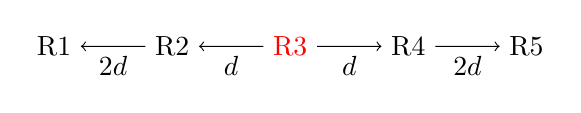
\begin{tikzpicture}[scale = 1.5]
\node (R1) at (.5, .5) {R1};
\node (R2) at (1.5,.5) {R2};
\node (R3) [color =  red]  at (2.5,.5) {R3};
\node (R4) at (3.5,.5) {R4};
\node (R5) at (4.5,.5) {R5};
\draw [->] (R3) -- (R2) node [midway, below] {$d$};
\draw [->] (R3) -- (R4) node [midway, below] {$d$};
\draw [->] (R2) -- (R1) node [midway, below] {$2d$};
\draw [->] (R4) -- (R5) node [midway, below] {$2d$};
\end{tikzpicture}
\end{figure}


When $\mW$ is an inverse distance matrix and its off-diagonal elements are of the form $1/d_{ij}$, where $d_{ij}$ is the distance between two spatial units $i$ and $j$, each row sum is

\begin{equation*}
  1/d + 1/d + 1/2d + 1/2d + .... = 2 \times (1/d + 1/2d + 1/3d + ....) 
\end{equation*}
%
representing a series that is not finite. This is perhaps the main motivation of why some empirical applications introduce a cut-off point $d^*$ such that $w_{ij}=0$ if $d_{ij}>d^*$. However, since the ratio $2 \times (1/d + 1/2d + 1/3d + ....)/ n \to 0$ as $n\to \infty$,  \cite{lee2004asymptotic}'s condition is satisfied, which implies that an inverse distance matrix without cut-off point does not necessarily have to be excluded in an empirical study for reasons of consistency. Thus, Assumption \ref{assu:ml_3} excludes cases where the row sums, $\sum_{j = 1}^n w_{ij}$, for $i = 1,...,n$, diverges to infinity at a rate equal to or faster than the rate of the sample size $n$, because the ML estimator would likely be inconsistent for those cases. Another case where $\left\lbrace h_n \right\rbrace$ is a bounded sequence is when we fixed the number of neighbors, such as in the case of $k$-neighbors approach. Nevertheless our distance example explains why it sometimes leads to numerical problems or unexpected outcomes in empirical applications. This is because the number of unit in the sample generally does not go to infinity, but is finite. 



%Assumptions~\ref{assu:ml_2} is always satisfied if $\left\lbrace h_n \right\rbrace$ is a bounded sequence. Think of $\mW_n$ as spatial weight matrix based on distances that is row-normalized. In this case the $i$th row

%\begin{equation*}
%  w_{i,n} = \frac{(d_{i1}, d_{i2}, ...,d_{in})}{\sum_{j = 1}^nd_{ij}}
%\end{equation*}

%where $d_{ij} > 0$ represents a function of the spatial distance of the $i$th and $j$th units in some space. For a row-normalized $\mW_n$, as $d_{i,j}$ are nonnegative constants and uniformly bounded, if the $\sum_{j = 1}^nd_{ij}, i = 1,...,n$ are uniformly bounded away from zero at the rate $h_n$ in the sense that $\sum_{j = 1}^nd_{ij} =O(h_n)$ uniformly in $i$ and $\lim \inf _{n\to \infty} h_n^{-1}\sum_{j = 1}^nd_{ij} > c$, where $c$ is a positive constant independent of $i$ and $n$, the implied normalized weights matrix will have the property of Assumption \ref{assu:ml_2}.


What if $h_n$ is unbounded? Under this case $\sum_{j = 1}^nd_{ij}$ is uniformly bounded away from zero at the rate $h_n$, where $\lim_{n\to \infty}h_n = \infty$. This particular case \textbf{rules out} cases where each unit has only a (fixed) finite number of neighbors even when the total number of unit increases to infinity. For example, it rules out the case where units correspond to counties and neighbors are defined as counties with contiguous border.

In which cases $h_n \to \infty$? This case requires that each unit in the limit has infinitely many neighbors. As stated by \cite{lee2002consistency}, in economic applications where either the neighbors of any unit are dense in a relevant space or each unit is influenced by many of its neighboring units, which represents a significant proportion of the total population units, it is likely that $\sum_{j = 1}^nd_{ij}$ will diverge and $(1/n)\sum_{j = 1}^nd_{ij}$ will converge as $n$ becomes large. Consider the case where $d_{ij} = 1 / \left|r_i - r_j\right|$, where $r_i$ is the proportion of state $i$'s population that is of African descent. As no state in USA has zero proportion of African-Americans in its population, $d_{ij}$ will be positive, and $(1/n)\sum_{j = 1}^nd_{ij}$ will be bounded away from zero and $\sum_{j = 1}^nd_{ij}$ will be likely to possess the $n$ rate of divergence in this example.

Another example occurs when all cross-sectional units are assumed to be neighbors of each other and are given equal weights. In that case all off-diagonal elements of the spatial weights matrix are $w_{ij} = 1$. Since the row and column sums are $n - 1$, these sums diverge to infinity as $n\to \infty$. In contrast to the previous case, however, $(n - 1)/ n\to 1$ instead of $0$ as $n\to\infty$. This implies that a spatial weight matrix that has equal weights and that is row-normalized subsequently, $w_{ij} - 1 / (n - 1)$ must be excluded for reasons of consistency since is satisfies neither \cite{lee2004asymptotic}'s and  \cite{kelejian1998generalized, kelejian1999generalized}'s condition. The alternative is a group interaction matrix, introduced by Case (1991). Here ``neighbors'' refer to farmers who live in the same district. Suppose that there are $R$ districts and there are $m$ farmers in each district. The sample size is $n = mR$. Case assumed that in a district, each neighbor of a farmer is given equal weight. In that case, $\mW_n  = \mI_R \otimes \mB_m$, where $\mB_m = (\vones_m\vones_m^\top - \mI_m)/(m - 1)$. For this example, $h_n = (m - 1)$ and $h_n/n = (m - 1) / (mR) = O(1/R)$. If sample size $n$ increases by increasing both $R$ and $m$, then $h_n$ goes to infinity and $h_n/n$ goes to zero as $n$ tends to infinity. Thus, this matrix satisfies \cite{lee2004asymptotic}'s condition. 



\begin{remark}
  Whether $\left\lbrace h_n \right\rbrace$ is a bounded or divergent sequence has interesting implications on the OLS estimation. The OLS estimators of $\vbeta$ and $\rho$ are inconsistent when $\left\lbrace h_n \right\rbrace$ is bounded, but they can be consistent when $\left\lbrace h_n \right\rbrace$ is divergent \citep[see][]{lee2002consistency}.
\end{remark}

In summary, when $\left\lbrace h_n \right\rbrace$ is a bounded sequence, it implies a cross sectional unit has only a small number of neighbors, where the spatial dependence is usually defined based on geographical implications. When $\left\lbrace h_n \right\rbrace$ is divergent, it corresponds to the scenario where each unit has a large number of neighbors that often emerges in empirical studies of social interactions or cluster sampling data. 

\begin{assumption}\label{assu:ml_4}
	The matrix $\mA_n$ is nonsingular.
\end{assumption}

Under Assumption \ref{assu:ml_4}, the SLM model (system) has the reduced form (equilibrium) given by Equation (\ref{eq:equilibrium_slm}) with the following expectation and variance:

\begin{eqnarray}
\E(\vy_n)   &=& \left(\mI_n - \rho_0\mW_n\right)^{-1}\mX_n\vbeta  = \mA_n^{-1}\mX_n\vbeta_0\\
\var(\vy_n) &=& \sigma^2_{0}\left(\mI_n - \rho_0\mW_n\right)^{-1}\left(\mI_n - \rho_0\mW_n\right)^{-1\top} = \sigma^2_0\mA_n^{-1}\mA_n^{-1\top}
\end{eqnarray}


\begin{assumption}\label{assu:ml_5}
	The sequences of matrices $\left\lbrace \mW_n \right\rbrace$ and $\left\lbrace \mA_n^{-1} \right\rbrace$ are uniformly bounded in both row and column sums 
\end{assumption}

The uniform boundedness of the matrices is a condition to limit the spatial correlation to a manageable degree. For example, it guarantees that the variances of $\vy_n$ are bounded as $n$ goes to infinity.

Technically, this assumes that $\left\lbrace \left\|\mW_n\right\|_1\right\rbrace$ and $\left\lbrace \left\|\mW_n\right\|_{\infty}\right\rbrace$ are bounded sequences. Formally, let $\mA_n$ be a square matrix. Using Definition \ref{def:Bounded_Matrices}, we say that the row and column sums of the sequences of matrices $\mA_n$ is bounded uniformly in absolute value if there exists a constant $c < \infty$ that does not depend on $N$ such that


\begin{equation*}
   \left\|\mA_n\right\|_{\infty} = \underset{1\leq i \leq n}{\sum_{j = 1} ^ N \left|a_{ij, N}\right|} < c, \quad  \left\|\mA_n\right\|_{1} = \underset{1\leq j \leq n}{\sum_{i = 1} ^ N \left|a_{ij, N}\right|} < c \quad \forall N
\end{equation*}

Why do we care about this? Because we need the variance goes to zero when the sample size goes to infinity in order to apply some consistency theorem.\footnote{Equivalently, this assumption rules out the unit root case in time series.}

\begin{lemma}[Uniform Boundedness of Matrices in Row and Column Sums]
  Suppose that the spatial weights matrix $\mW_n$ is a non-negative matrix with its $(i,j)$th element being 
  
  \begin{equation*}
    w_{n,ij} = \frac{d_{ij}}{\sum_{l = 1}^nd_{il}}
  \end{equation*}
  
  and $d_{ij}>0$ for all $i,j$.
  
  \begin{enumerate}
    \item If the row sums $\sum_{j = 1}^nd_{ij}$ are bounded away from zero at the rate $h_n$ uniformly in $i$, and the column sums $\sum_{i = 1}^nd_{ij}$ are $O(h_n)$ uniformly in $j$, then $\left\lbrace \mW_n \right\rbrace$  are uniformly bounded in column sums.
    \item (Symmetric Matrix) If $d_{ij} = d_{ji}$ for all $i$ and $j$ and the row sums $\sum_{j = 1}^nd_{ij}$ are $O(h_n)$ and bounded away from zero at the rate $h_n$ uniformly in $i$, then $\left\lbrace \mW_n \right\rbrace$  are uniformly bounded in column sums.
  \end{enumerate}
\end{lemma}

\begin{assumption}\label{assu:ml_6}
	The elements of $\mX_n$ are uniformly bounded constants for all $n$. The $\lim_{n\to \infty}\mX_n^\top\mX_n/n$ exists and is nonsingular. 
\end{assumption}

This rules out multicollinearity among the regressors. Note also that we are assuming that $\mX_n$ is \textbf{nonstochastic}. If $\mX_n$ were stochastic, then we will require:

\begin{equation*}
  \plim_{n\to \infty}\mX_n^\top\mX_n/ n,
\end{equation*}

to exists.

\begin{assumption}\label{assu:ml_7}
	${\mA_n^{-1}(\rho)}$ are uniformly bounded in either row or column sums, uniformly in $\rho$ in a compact parameter space $\mP$. The true parameter $\rho_0$ is in the interior of $\mP$
\end{assumption}

This assumption is needed to deal with the nonlinearity of $\log \left|\left(\mI_n - \rho \mW\right)^{-1}\right|$ in the log-likelihood function. Recall that if $\left\| \mW\right\| < 1$, then $\mI_n - \rho\mW_n$ is invertible for all $n$. Then if $\left\| \mW\right\| < 1$, then the sequence of matrices $\left\|\left(\mI_n- \mW_n\right)^{-1}\right\|$ are uniformly bounded in any subset of $(-1, 1)$ bounded away from the boundary. As we previously see, if $\mW$ is row-standardized $\left(\mI_n- \mW\right)^{-1}$ is uniformly bounded in row sums norm uniformly in any closed subset of $(-1, 1)$. Therefore, $\mP$ from Assumption~\ref{assu:ml_7} can be considered as a single closed set contained in (-1, 1).

What if $\mW$ is not row-normalized but its eigenvalues are real? Then, the Jacobian of $\left|\left(\mI_n- \mW\right)^{-1}\right|$ will be positive if $-1/\omega_{min} < \rho < 1/\omega_{max}$, where $\omega_{min}$ and $\omega_{max}$ are the minimum and maximum eigenvalues of $\mW$, and $\mP$ will be a closed interval contained in $(-1/\omega_{min}, 1/\omega_{max})$ for all $n$. Thus, Assumption~\ref{assu:ml_7} rules out models where $\rho_0$ is close to -1 and 1.  

Now, noting that:


\begin{equation}
	\begin{aligned}
	\vy_n & = \mX_n\vbeta_0 + \rho_0\mW_n\vy_n + \vepsi_n \\
	      & = \mX_n\vbeta_0 + \rho_0\mW_n\left[\mA^{-1}_n\mX_n\vbeta_0 + \mA^{-1}_n\vepsi_n\right] + \vepsi_n \\
	      & = \mX_n\vbeta_0 + \rho_0\mW_n\mA^{-1}_n\mX_n\vbeta_0 + \rho_0\mW_n\mA^{-1}_n\vepsi_n + \vepsi_n \\
	      & = \mX_n\vbeta_0 + \rho_0\mW_n\mA^{-1}_n\mX_n\vbeta_0  + \left(\mI_n + \rho_0\mW_n\mA^{-1}_n\right)\vepsi_n \\
	      & = \mX_n\vbeta_0 + \rho_0\mC_n\mX_n\vbeta_0  + \left(\mI_n + \rho_0\mC_n\right)\vepsi_n \\
	      & = \mX_n\vbeta_0 + \rho_0\mC_n\mX_n\vbeta_0  +\mA_n^{-1}\vepsi_n
	\end{aligned}
\end{equation}

because $\mI_n + \rho_0\mC_n = \mA_n^{-1}$ (see Exercise  \ref{lab:4.6}), where $\mC_n=\mW_n\mA_n^{-1}$.


\begin{assumption}\label{assu:ml_8}
		The
		\begin{equation*}
			\lim_{n\to \infty}\frac{1}{n}\left(\mX_n, \mC_n\mX_n\vbeta_0\right)'\left(\mX_n, \mC_n\mX_n\vbeta_0\right)
		\end{equation*}
		 exists and is nonsingular.
\end{assumption}

This is a sufficient condition for global identification of $\vtheta_0$


\begin{theorem}[Consistency]\label{teorem:Consistency_ML}
	Under assumption \ref{assu:ml_1}-\ref{assu:ml_8}, $\vtheta_0$ is globally identifiable and $\widehat{\vtheta}_n$ is a consistent estimator of $\vtheta_0$.
\end{theorem}

The proof is given in \cite{lee2004asymptotic}. Identification of $\rho_0$ can be based on the maximum values of the concentrated log-likelihood function $Q_n(\rho) / n$. With identification and uniform convergence of $\left[\log L_n(\rho) - Q_n(\rho)\right] / n$ to zero on $\mP$, consistency of the QMLE $\widehat{\vtheta}_n$ follows.

For a proof without compactness of the parameter space see \cite{liu2022consistency}.

%=====================================
\subsection{Asymptotic Normality}
%=====================================

To derive the asymptotic distribution of the QML and ML we need the asymptotic behavior of the gradient. Taking a Taylor series expansion around $\vtheta_0$ of $\partial \log L_n(\widehat{\vtheta}_n)/ \partial \vtheta = 0$ at $\vtheta_0$, we get:

\begin{equation}
  \frac{\partial \log L_n(\widehat{\vtheta}_n)}{\partial \vtheta} =  \frac{\partial \log L_n(\vtheta_0)}{\partial \vtheta} + \frac{\partial^2 \log L_n(\widetilde{\vtheta}_n)}{\partial \vtheta \partial \vtheta^\top}(\widehat{\vtheta}_n - \vtheta_0),
\end{equation}
%
where $\widetilde{\vtheta}_n = \alpha_n \widehat{\vtheta}_n + (1 - \alpha_n)\vtheta_0$ and $\alpha_n\in \left[ 0, 1\right]$, therefore:

\begin{equation}\label{eq:sampling-error-ml}
  \sqrt{n}(\widehat{\vtheta}_n - \vtheta_0) = - \left[\frac{1}{n}\frac{\partial^2 \log L_n(\widetilde{\vtheta}_n)}{\partial \vtheta \partial \vtheta^\top}\right]^{-1}\frac{1}{\sqrt{n}}\frac{\partial \log L_n(\vtheta_0)}{\partial \vtheta}.
\end{equation}

As standard in asymptotic theory of ML, we need to show that the first element of the rhs of (\ref{eq:sampling-error-ml}) converges to something. We also need to find the limiting distribution of $\frac{1}{\sqrt{n}}\frac{\partial \log L_n(\vtheta_0)}{\partial \vtheta}$. Recall that the first-order derivatives of the log-likelihood function at $\vtheta_0$ are given by (see Section \ref{sec:score_sml}):

\begin{equation}
	\frac{1}{\sqrt{n}}\frac{\partial \log L_n(\vtheta_0)}{\partial \vbeta} = \frac{1}{\sigma^2_0\sqrt{n}}\mX_n^\top\vepsi_n
\end{equation}	


\begin{equation}
\frac{1}{\sqrt{n}}\frac{\partial \log L_n(\vtheta_0)}{\partial \sigma^2} = \frac{1}{2\sigma_0^4\sqrt{n}}\left(\vepsi_n'\vepsi_n - n\sigma_0^2\right)
\end{equation}

and

\begin{equation}\label{eq:asy_der_rho}
	\frac{1}{\sqrt{n}}\frac{\partial \log L_n(\vtheta_0)}{\partial \rho} = \frac{1}{\sigma_0^2\sqrt{n}}(\mC_n\mX_n\vbeta_0)^\top \vepsi_n + \frac{1}{\sigma_0^2\sqrt{n}}(\vepsi_n^\top\mC_n\vepsi_n - \sigma_0^2\tr(\mC_n))
\end{equation}

As explained by \citet[][pag. 1905]{lee2004asymptotic}, these are linear and quadratic functions of $\vepsi_n$. In particular, the asymptotic distribution of (\ref{eq:asy_der_rho}) may be derived from central limit theorem for linear-quadratic forms. The matrix $\mC_n$ is uniformly bounded in row sums. As the elements of $\mX_n$ are bounded, the elements of $\mC_n\mX_n\vbeta_0$ for all $n$ are uniformly bounded by Lemma \ref{lemma:bounded_lemma}. With the existence of high order moments of $\epsilon$ in Assumption \ref{assu:ml_1}, the central limit theorem for quadratic forms of double arrays of \cite{kelejian2001asymptotic} can be applied and the limit distribution of the score vector follows.

%Recall that we need to show that:


%\begin{equation}
%  \frac{1}{\sqrt{n}}\frac{\partial \log L_n(\vtheta_0)}{\partial \vtheta} \dto \rN(\vzeros, \mSigma)\quad \mbox{where}\quad \mSigma_{\vtheta} = \E\left[\left(\frac{\partial \log L_n(\vtheta_0)}{\partial \vtheta}\right)\left(\frac{\partial \log L_n(\vtheta_0)}{\partial \vtheta}\right)^\top\right]
%\end{equation}


Since $\E\left[(1 / \sqrt{n}) \partial \log L_n /\partial \vtheta\right]  = \vzeros$,  the variance matrix of $(1 / \sqrt{n}) \partial \log L_n /\partial \vtheta$ is:

\begin{equation}
  \E\left[\frac{1}{\sqrt{n}}\frac{\partial \log L_n (\vtheta_0)}{\partial \vtheta}\cdot\frac{1}{\sqrt{n}}\frac{\partial \log L_n (\vtheta_0)}{\partial \vtheta^\top}\ \right] = - \E\left(\frac{1}{n} \frac{\partial \log L_n(\vtheta)}{\partial \vtheta \partial \vtheta^\top}\right) + \mOmega_{\vtheta, n},
\end{equation}
%
where 

\begin{equation}\label{eq:expected-hessian-slm-asy}
- \E\left(\frac{1}{n} \frac{\partial \log L_n(\vtheta)}{\partial \vtheta \partial \vtheta^\top}\right)= 
	\begin{pmatrix}
	\frac{1}{\sigma^2n}(\mX_n^\top \mX_n) & \vzeros^\top & \frac{1}{\sigma^2n} \mX_n^\top (\mC_n\mX_n\vbeta) \\
		 &  \frac{1}{2\sigma^4} & \frac{1}{\sigma^2n} \tr(\mC_n)\\
		 &  & \frac{1}{n}\tr(\mC^s_n\mC_n) + \frac{1}{\sigma^2n}(\mC_n\mX_n\vbeta)^\top(\mC_n\mX_n\vbeta)
	\end{pmatrix} 
\end{equation}
%
and $\mC^s_n = \mC_n + \mC_n^\top$. Equation \ref{eq:expected-hessian-slm-asy} represents the average Hessian matrix (or information matrix when $\vepsi$'s are \textbf{normal}). The matrix $ \mOmega_{\vtheta, n}$ is a matrix with the second, third, and fourth moments of $\vepsi$. If $\vepsi_n$ is normally distributed, then $\mOmega_{\vtheta, n} = \vzeros$. Derivation of \ref{eq:expected-hessian-slm-asy} is given in Appendix \ref{appendix-EH-sml}.



\begin{theorem}[Asymptotic Normality]
Under Assumptions \ref{assu:ml_1}-\ref{assu:ml_8}, 

\begin{equation}
  \sqrt{n}\left(\widehat{\vtheta}_n- \vtheta_0\right)\dto \rN\left(\vtheta, \mSigma_{\vtheta}^{-1} + \mSigma_{\vtheta}^{-1}\mOmega_{\vtheta}\mSigma_{\vtheta}^{-1}\right),
\end{equation}
%
where $\mOmega_{\vtheta} = \lim_{n\to\infty}\mOmega_{\vtheta, n}$ and

\begin{equation}
  \mSigma_{\vtheta}= - \lim_{n\to\infty} \E\left[\frac{1}{n}\frac{\partial^2 \log L_n(\vtheta_0)}{\partial \vtheta \partial \vtheta^\top}\right],
\end{equation}
which are assumed to exists. If the $\epsilon_i$'s are \textbf{normally distributed}, then:

\begin{equation}
  \sqrt{n}\left(\widehat{\vtheta}_n- \vtheta_0\right)\dto \rN\left(\vtheta, \mSigma_{\vtheta}^{-1}\right).
\end{equation}
\end{theorem}


%The following lemmas and statements summarize some basic properties on spatial weight matrices and some law of large numbers and central limit theorems on linear and quadratic forms. For proof of these lemmas see \cite{lee2004asymptotic}' appendix. The error term $\vepsi_n$ are assumed to be i.i.d. with zero mean and finite variance $\sigma_0^2$ according to Assumption \ref{assu:ml_1}. For quadratic forms involving $\vepsi$, the fourth moment $\mu_4$ for the $\vepsi$'s is assumed to exists. 



% \begin{lemma}
% Suppose that $\left\lbrace \mA_n\right\rbrace$ is a sequence of symmetric matrices with row and column sums uniformly bounded and $\left\lbrace \vb_n\right\rbrace$ is  a sequence of constant  vectors with its elements uniformly bounded. The moment $\E\left(\left|\vepsi\right|\right)$ for some $\delta>0$ of $\vepsi$ exists. Let $\sigma^2_{Q_n}$ be the variance of $Q_n$ where $Q_n = \vb_n^\top\vepsi + \vepsi^\top\mA_n\vepsi_n -\sigma^2_0$. Assume that the variance $\sigma^2_{Q_n}$ is $O(n/h_n)$ with $\left\lbrace(h_n / n)\sigma^2_{Q_n}\right\rbrace$ bounded away from zero, the elements of $\mA_n$ are uniform order $O(1/h_n)$ and the elements of $\vb_n$ of uniform order $O(1/\sqrt{h_n})$. If $\lim_{n\to\infty}\frac{h_n^{1 + 2/\delta}}{n} = 0$, then $Q_n/\sigma_{Q_n}\dto \rN(0,1)$
% \end{lemma}

%-------------------------------------------------------
\begin{proof}[Sketch of Proof Asymptotic Normality] We will sketch the proof of asymptotic normality assuming consistency (Theorem \ref{teorem:Consistency_ML}) and normality of the error terms. The sketch consists in the following steps: 
\begin{enumerate}
  \item First, we need to show that:
  
    \begin{equation*}
    \mSigma_{\vtheta} = - \lim_{n\to\infty} \E\left[\frac{1}{n}\frac{\partial^2 \log L_n(\vtheta_0)}{\partial \vtheta \partial \vtheta^\top}\right]
    \end{equation*}
    %
    is non-singular. To show this is beyond the scope of this class notes. We will take this as given. 
  \item Now we will show that 
  
   \begin{equation*}
    \frac{1}{n}\frac{\partial^2 \log L_n(\widetilde{\vtheta}_n)}{\partial \vtheta \partial \vtheta^\top}\pto \frac{1}{n}\frac{\partial^2 \log L_n(\vtheta_0)}{\partial \vtheta \partial \vtheta^\top}
   \end{equation*}
   
   Recall that the second derivatives are given by Equations (\ref{eq:sar_der_beta_beta})-(\ref{eq:sar_der_rho_rho}).
   
   By Assumption \ref{assu:ml_6} (No asymptotic multicolinearity), we know that  $\lim_{n\to\infty}\frac{1}{n}\mX_n^\top\mX_n$ exists, therefore $\mX_n^\top\mX_n = O(n)$ so that $\mX_n^\top\mX_n/n = O(1)$ (Lemma \ref{lemma:bounde_ON})\footnote{Since $\lim_{n\to\infty}\frac{1}{n}\mX_n^\top\mX_n$ exists, then, each of its elements is o(1) and hence O(1). In other words, $\frac{1}{n}\mX_n^\top\mX_n$ is a bounded matrix.}   and $\widetilde{\sigma}^2_n\pto \sigma_0^2$ from consistency, then from Equation (\ref{eq:sar_der_beta_beta}), we have:
   
   \begin{equation*}
    \begin{aligned}
    \frac{1}{n}\frac{\partial^2 \log L_n(\widetilde{\vtheta}_n)}{\partial \vbeta \partial \vbeta^\top} - \frac{1}{n}\frac{\partial^2 \log L_n(\vtheta_0)}{\partial \vbeta \partial \vbeta^\top} & = - \frac{1}{\widetilde{\sigma}^2_n}\frac{(\mX^\top_n \mX_n)}{n} + \frac{1}{\sigma^2_0}\frac{(\mX^\top_n \mX_n)}{n} \\
    & = \underbrace{\left(\frac{1}{\sigma^2_0} - \frac{1}{\widetilde{\sigma}^2_n}\right)}_{o_p(1)}\underbrace{\frac{(\mX^\top_n \mX_n)}{n}}_{O(1)} \\
    & = o_p(1)O(1)  \\
    & = o_p(1)
    \end{aligned}
   \end{equation*}
   
  By Lemma \ref{lemma:limiting-distr-lee}, we obtain the following results:
   
   \begin{equation*}
    \begin{aligned}
      \frac{1}{n}\mX_n^\top\mC_n^\top\vepsi_n & =o_p(1) \\
      \frac{1}{n}\mX_n^\top\mC_n^\top\mC_n\vepsi_n & = o_p(1)
    \end{aligned}
   \end{equation*}
   
   It follows that:
   
   \begin{equation*}
    \begin{aligned}
      \frac{1}{n}\mX_n^\top\mW_n^\top\vy_n & = \frac{1}{n}\mX_n^\top\mC_n\mX_n\vbeta_0 + o_p(1) \\
      \frac{1}{n}\vy_n^{\top}\mW_n^{\top}\vepsi_n &= \frac{1}{n}\vepsi_n^\top\mC_n^{\top}\vepsi_n + o_p(1) \\
      \frac{1}{n}\vy_n^\top\mW_n^\top\mW_n\vy_n & = \frac{1}{n}\left(\mX_n\vbeta_0\right)^\top\mC_n^\top\mC_n\mX_n\vbeta_0 + \frac{1}{n}\vepsi_n^\top\mC_n^\top\mC_n\vepsi_n + o_p(1)
    \end{aligned}
   \end{equation*}
   
   
   As $\mX_n^\top\mW_n\vy_n /n = O_p(1)$ (it convergences to something in distribution), it follows from Equation (\ref{eq:sar_der_beta_rho}):
   
   \begin{equation*}
    \begin{aligned}
    \frac{1}{n}\frac{\partial^2 \log L_n(\widetilde{\vtheta}_n)}{\partial \vbeta \partial \rho} - \frac{1}{n}\frac{\partial^2 \log L_n(\vtheta_0)}{\partial \vbeta \partial \rho} & = - \frac{1}{\widetilde{\sigma}^2_n}\frac{(\mX^\top_n \mW_n\vy_n)}{n} + \frac{1}{\sigma^2_0}\frac{(\mX^\top_n \mW_n\vy_n)}{n} \\
    & = \underbrace{\left(\frac{1}{\sigma^2_0} - \frac{1}{\widetilde{\sigma}^2_n}\right)}_{o_p(1)}\underbrace{\frac{(\mX^\top_n \mW_n\vy_n)}{n}}_{O_p(1)} \\
    & = o_p(1)O_p(1)  = o_p(1)
    \end{aligned}
   \end{equation*} 
   
   The following identity will be useful:
   
   \begin{equation}\label{eq:error_slm_lee}
    \begin{aligned}
    \vepsi(\widetilde{\vdelta}_n) & = \vy_n - \mX_n\widetilde{\vbeta}_n - \widetilde{\rho}_n\mW_n\vy_n +(\vepsi(\vdelta_0) -  \vepsi(\vdelta_0)) \\
    & = \vy_n - \mX_n\widetilde{\vbeta}_n - \widetilde{\rho}_n\mW_n\vy_n - \vy_n + \mX_n\vbeta_0 - \rho_0\mW_n\vy_n + \vepsi_n(\vdelta_0) \\
    & = \mX_n(\vbeta_0 - \widetilde{\vbeta}_n) + (\rho_0 - \widetilde{\rho}_n)\mW_n\vy_n + \vepsi_n(\vdelta_0) 
    \end{aligned}
   \end{equation}
   
   Then, taking into account Equation (\ref{eq:sar_der_beta_sigma}) and using our result in Equation (\ref{eq:error_slm_lee}) yields:
   
      \begin{equation*}
    \begin{aligned}
    \frac{1}{n}\frac{\partial^2 \log L_n(\widetilde{\vtheta}_n)}{\partial \vbeta \partial \sigma^2} - \frac{1}{n}\frac{\partial^2 \log L_n(\vtheta_0)}{\partial \vbeta \partial \sigma^2} & = - \frac{1}{\widetilde{\sigma}^4_n} \frac{\mX_n^\top \vepsi(\widetilde{\vdelta}_n)}{n}+  \frac{1}{\sigma^4_0} \frac{\mX^\top_n \vepsi_n(\vdelta_0)}{n}. \\
    & = - \frac{1}{\widetilde{\sigma}^4_n}\frac{1}{n}\mX^\top\left(\mX_n(\vbeta_0 - \widetilde{\vbeta}_n) + (\rho_0 - \widetilde{\rho}_n)\mW_n\vy_n + \vepsi_n(\vdelta_0) \right)+  \\
    & \quad + \frac{1}{\sigma^4_0} \frac{\mX^\top_n \vepsi_n(\vdelta_0)}{n} \\
  & = \frac{1}{\widetilde{\sigma}^4_n}\frac{1}{n}\mX^\top\mX_n(\vbeta_0 - \widetilde{\vbeta}_n) - \frac{1}{\widetilde{\sigma}^4_n}\frac{1}{n}\mX^\top\mW_n\vy_n(\rho_0 - \widetilde{\rho}_n) - \frac{1}{\widetilde{\sigma}^4_n}\frac{1}{n}\mX^\top \vepsi_n(\vdelta_0) + \\
   & \quad + \frac{1}{\sigma^4_0} \frac{\mX^\top_n \vepsi_n(\vdelta_0)}{n} \\
  & = \left(\frac{1}{\sigma^4_0} - \frac{1}{\widetilde{\sigma}^4_n}\right)\frac{\mX^\top_n \vepsi_n(\vdelta_0)}{n} + \frac{\mX^\top_n\mX_n}{n\widetilde{\sigma}^4_n}(\vbeta_0 - \widetilde{\vbeta}_n) + \frac{\mW_n^\top\mW_n\vy_n}{n\widetilde{\sigma}^4_n}(\rho_0 - \widetilde{\rho}_n) \\
  & = o_p(1)O_p(1) + O(1)o_p(1) + O_p(1)o_p(1) \\
  & = o_p(1)
    \end{aligned}
   \end{equation*}
   
   From Equation (\ref{eq:sar_der_rho_rho}), we know that:
   
   \begin{equation*}
   \frac{\partial \log L_n(\vtheta) }{\partial \rho ^2} = - \tr\left[(\mC_n(\rho))^2\right] - \frac{1}{\sigma^2}(\vy_n^{\top}\mW^{\top}_n\mW_n\vy_n)\quad \mbox{where}\quad \mC_n(\rho) = \mW_n\mA_n(\rho)^{-1}
   \end{equation*}
   
   From Mean Value Theorem around of  $\tr\left[(\mC_n(\widetilde{\rho}_n))^2\right]$ around $\rho_0$:
   
   \begin{equation*}
    \begin{aligned}
    \tr\left[(\mC_n(\widetilde{\rho}_n))^2\right] & = \tr\left[(\mC_n(\rho_0))^2\right]+ 2\tr\left[(\mC_n(\bar{\rho}))^3\right](\rho_0 - \widetilde{\rho}_n) \\
    \tr\left[(\mC_n(\widetilde{\rho}_n))^2\right] - \tr\left[(\mC_n(\rho_0))^2\right] & = 2\tr\left[(\mC_n(\bar{\rho}))^3\right](\rho_0 - \widetilde{\rho}_n)
    \end{aligned}
   \end{equation*}
   
   Then:
   
   \begin{equation*}
    \begin{aligned}
    \frac{1}{n}\frac{\partial^2 \log L_n(\widetilde{\vtheta}_n)}{\partial \rho^2} - \frac{1}{n}\frac{\partial^2 \log L_n(\vtheta_0)}{\partial\rho^2} & = \underbrace{2\frac{1}{n}\tr\left[(\mC_n(\bar{\rho}))^3\right]}_{O(n/h_n)} \underbrace{(\rho_0 - \widetilde{\rho}_n)}_{o_p(1)} + \underbrace{\left(\frac{1}{\sigma^2_0} - \frac{1}{\widetilde{\sigma}^2_n}\right)}_{o_p(1)}\underbrace{\frac{\vy_n^{\top}\mW^{\top}_n\mW_n\vy_n}{n}}_{O_p(n/h_n)} = o_p(1)
    \end{aligned}
   \end{equation*}
   
   Note that $\mC_n(\bar{\rho})$ is uniformly bounded in row and column sums uniformly in a neighborhood of $\rho_0$ by  Assumption \ref{assu:ml_5} and \ref{assu:ml_7}. Note that $\tr\left[(\mC_n(\bar{\rho}))^3\right] = O(n/h_n)$ by Lemma 
   
  Considering Equation (\ref{eq:sar_der_sigma_rho}):
   
   
    \begin{equation*}
    \begin{aligned}
    \frac{1}{n}\frac{\partial^2 \log L_n(\widetilde{\vtheta}_n)}{\partial \sigma^2 \partial \rho} - \frac{1}{n}\frac{\partial^2 \log L_n(\vtheta_0)}{\partial \sigma^2 \partial \rho}& = -\frac{1}{\widetilde{\sigma}^4}\frac{1}{n}\vy_n^\top\mW_n^\top\vepsi_n(\widetilde{\vdelta}_n) + \frac{1}{\sigma^4}\frac{1}{n}\vy_n^\top\mW_n^\top\vepsi_n(\vdelta_n)\\
    & = -\frac{1}{\widetilde{\sigma}^4}\frac{1}{n}\vy_n^\top\mW_n^\top\left[\mX_n(\vbeta_0 - \widetilde{\vbeta}_n) + (\rho_0 - \widetilde{\rho}_n)\mW_n\vy_n + \vepsi_n(\vdelta_0)\right] + \\
    &  \frac{1}{\sigma^4}\frac{1}{n}\vy_n^\top\mW_n^\top\vepsi_n(\vdelta_n) \\
    &= -\frac{1}{\widetilde{\sigma}^4}\frac{1}{n}\vy_n^\top\mW_n^\top\mX_n(\vbeta_0 - \widetilde{\vbeta}_n)  + \frac{1}{\widetilde{\sigma}^4}\frac{1}{n}\vy_n^\top\mW_n^\top\mW_n\vy_n(\widetilde{\rho}_n-\rho_0) + \\
    & \left(\frac{1}{\sigma^4}-\frac{1}{\widetilde{\sigma}^4}\right)\frac{1}{n}\vy_n^\top\mW_n^\top\vepsi_{n} \\
    & = o_p(1)
    \end{aligned}
   \end{equation*}
   
    Note the following:
   
   \begin{equation*}
    \begin{aligned}
    \frac{1}{n}\vepsi(\widetilde{\vdelta})^\top \vepsi(\widetilde{\vdelta}) & = \left(\widetilde{\vbeta}_n - \vbeta_0\right)^\top\frac{\mX_n^\top\mX_n}{n} + (\widetilde{\rho}_n -\rho_0)^2\frac{\vy_n^\top\mW_n^\top\mW_n\vy_n}{n} + \frac{\vepsi_n^{\top}\vepsi_n}{n} + \\
    & 2(\widetilde{\rho}_n -\rho_0)\left(\widetilde{\vbeta}_n - \vbeta_0\right)^\top\frac{\mX_n^\top\mW_n\vy_n}{n} + 2\left(\vbeta_0-\widetilde{\vbeta}_n\right)^\top\frac{\mX_n^\top\vepsi_n}{n} + 2(\rho_0-\widetilde{\rho}_n)\frac{\vy_n^\top\mW_n^\top\vepsi_n}{n} \\
    & = \frac{\vepsi_n^{\top}\vepsi_n}{n} + o_p(1)
    \end{aligned}
   \end{equation*}
   
   
   Finally, considering the second derivative in Equation (\ref{eq:sar_der_sigma_sigma})
   
   \begin{equation*}
    \begin{aligned}
      \frac{1}{n}\frac{\partial^2 \log L(\widetilde{\vtheta})}{\partial (\sigma^2)^2} -	\frac{1}{n}\frac{\partial^2 \log L(\vtheta_0)}{\partial (\sigma^2)^2}  & = \frac{1}{2(\widetilde{\sigma}^2) ^2} - \frac{1}{(\widetilde{\sigma}^2)^3} \frac{1}{n}\vepsi(\widetilde{\vdelta})^\top \vepsi(\widetilde{\vdelta}) -\frac{1}{2(\sigma^2) ^2} + \frac{1}{(\sigma^2)^3} \frac{1}{n}\vepsi^\top \vepsi \\
      & = \frac{1}{2}\left(\frac{1}{\widetilde{\sigma}^2) ^2}-\frac{1}{(\sigma^2) ^2}\right)- \frac{1}{(\widetilde{\sigma}^2)^3} \frac{1}{n}\vepsi(\widetilde{\vdelta})^\top \vepsi(\widetilde{\vdelta}) + \frac{1}{(\sigma^2)^3} \frac{1}{n}\vepsi^\top \vepsi \\
      & = \frac{1}{2}\left(\frac{1}{\widetilde{\sigma}^2) ^2}-\frac{1}{(\sigma^2) ^2}\right)- \frac{1}{(\widetilde{\sigma}^2)^3} \left(\frac{\vepsi_n^{\top}\vepsi_n}{n} + o_p(1)\right)+ \frac{1}{(\sigma^2)^3} \frac{1}{n}\vepsi^\top \vepsi \\
      & = \frac{1}{2}\left(\frac{1}{\widetilde{\sigma}^2) ^2}-\frac{1}{(\sigma^2) ^2}\right)+ \left(\frac{1}{(\sigma^2)^3} -\frac{1}{(\widetilde{\sigma}^2)^3}\right)\frac{\vepsi_n^{\top}\vepsi_n}{n} + o_p(1) \\
      & = o_p(1)
    \end{aligned}
   \end{equation*}
   

   
   \item Now, we need to show that:
   
   \begin{equation}
     \frac{1}{n}\frac{\partial^2 \log L_n(\vtheta_0)}{\partial \vtheta \partial \vtheta^\top}\pto \E\left[\frac{1}{n}\frac{\partial^2 \log L_n(\vtheta_0)}{\partial \vtheta \partial \vtheta^\top}\right]
   \end{equation}
   
   Form Appendix \ref{appendix-EH-sml}, we know that:
   
   \begin{equation*}
    \begin{aligned}
     \E\left[\frac{1}{n}\left.\frac{\partial^2  \log L(\vtheta_0)}{\partial \vbeta \partial \vbeta^\top} \right|\mW, \mX\right] & = -\frac{1}{\sigma^2_0}\frac{1}{n}(\mX^\top\mX) \\
     \E\left[\frac{1}{n}\left.\frac{\partial^2  \log L(\vtheta_0)}{\partial \vbeta \partial \sigma^2} \right|\mW, \mX\right] & = \vzeros \\
      \E\left[\frac{1}{n}\left.\frac{\partial^2  \log L(\vtheta_0)}{\partial \vbeta \partial \rho} \right|\mW, \mX\right] & = - \frac{1}{\sigma^2_0} \frac{1}{n}\mX^\top\mC\mX\vbeta_0 \\
      \E\left[\frac{1}{n}\left.\frac{\partial^2 \log L(\vtheta_0)}{\partial (\sigma^2)^2}\right|\mW, \mX\right] & = - \frac{1}{2\sigma^4_0}  \\
      \E\left[\frac{1}{n}\left.\frac{\partial^2 \log L(\vtheta_0)}{\partial \sigma^2 \partial \rho}\right|\mW,\mX\right] & = - \frac{1}{n}\tr(\mC)/\sigma^2_0 \\
      \E\left[\frac{1}{n}\left.\frac{\partial^2 \log L(\vtheta_0)}{\partial \rho ^2}\right|\mW, \mX\right] & = - \frac{1}{n}\tr(\mC^s\mC) - \frac{1}{\sigma^2_0}\frac{1}{n}(\mC\mX\vbeta_0)^\top(\mC\mX\vbeta_0)
    \end{aligned}
   \end{equation*}
   
   All these expectations exist in the limit by Assumption \ref{assu:ml_8} and Lemma \ref{lemma:second-mom-lee}-\ref{lemma:O-lemma-lee}. Then, by nonsingularity of $\E\left[\mH(\vw_i;\vtheta)\right]$, we can say that 
   
   \begin{equation*}
   \left(\frac{1}{n}\mH(\vw;\widehat{\vtheta})\right)^{-1}\pto \E\left[\mH(\vw;\vtheta_0)\right]^{-1}
   \end{equation*}
   

   % Lemma \ref{lemma:second-mom-lee} implies that $\E(\vepsi_n^\top\mC_n^\top\vepsi_n)=\sigma_0^2\tr(\mC_n)$ and, under normality assumption, 
   % 
   % \begin{equation}
   % \var\left(\frac{1}{n}\vepsi_n^\top\mC_n^\top\vepsi_n\right) = \frac{\sigma_{0}^4}{n^2}\left[\tr\left(\mC_n\mC_n^\top\right) +\tr(\mC_n^2)\right] =O\left(\frac{1}{nh_n}\right)
   % \end{equation}
   % 
   % Similarly, $\E(\vepsi_n^\top\mC_n^\top\mC_n\vepsi_n)=\sigma_0^2\tr(\mC_n^\top\mC_n)$ and, under normality assumption, 
   % 
   % \begin{equation}
   % \var\left(\frac{1}{n}\vepsi_n^\top\mC_n^\top\mC_n\vepsi_n\right) =O\left(\frac{1}{nh_n}\right)
   % \end{equation}
   % 
   % By the law of large numbers $\frac{1}{n}\vepsi_n^\top\vepsi_n\pto \sigma^2_0$. With these properties the convergence results follows. 
   
   
   \item Recall that the first-order derivatives of the log-likelihood function at $\vtheta_0$ are given by:
   
  \begin{equation*}
   \frac{1}{\sqrt{n}}\frac{\partial \log L_n(\vtheta_0)}{\partial \vtheta} = \begin{pmatrix}
   \frac{1}{\sigma^2_0\sqrt{n}}\mX_n^\top\vepsi_n\\
   \frac{1}{2\sigma_0^4\sqrt{n}}\left(\vepsi_n'\vepsi_n - n\sigma_0^2\right) \\
   \frac{1}{\sigma_0^2\sqrt{n}}(\mC_n\mX_n\vbeta_0)^\top \vepsi_n + \frac{1}{\sigma_0^2\sqrt{n}}(\vepsi_n^\top\mC_n\vepsi_n - \sigma_0^2\tr(\mC_n))
   \end{pmatrix}
  \end{equation*}


As explained by \citet[][pag. 1905]{lee2004asymptotic}, these are linear and quadratic functions of $\vepsi_n$. In particular, the asymptotic distribution of $\frac{1}{\sqrt{n}}\frac{\partial \log L_n(\vtheta_0)}{\partial \vtheta}$ may be derived from central limit theorem for linear-quadratic forms. The matrix $\mC_n$ is uniformly bounded in row sums. As the elements of $\mX_n$ are bounded, the elements of $\mC_n\mX_n\vbeta_0$ for all $n$ are uniformly bounded by Lemma \ref{lemma:bounded_lemma}. With the existence of high order moments of $\epsilon$ in Assumption \ref{assu:ml_1}, the central limit theorem for quadratic forms of double arrays of \cite{kelejian2001asymptotic} can be applied and the limit distribution of the score vector follows.
   
Since $\E\left[(1 / \sqrt{n}) \partial \log L_n /\partial \vtheta\right]  = \vzeros$,  the variance matrix of $(1 / \sqrt{n}) \partial \log L_n /\partial \vtheta$ \textbf{under normality} is given by Equation \eqref{eq:expected-hessian-slm-asy}. Then:


\begin{equation}
 \frac{1}{\sqrt{n}}\frac{\partial \log L_n(\vtheta_0)}{\partial \vtheta} \dto \rN(\vzeros, -\E\left[\mH(\vw_i;\vtheta)\right]), 
\end{equation}
%
and:

\begin{equation*}
\sqrt{n}(\widehat{\vtheta}_n - \vtheta_0)\dto -\E\left[\mH(\vw_i;\vtheta)\right]^{-1}\rN(\vzeros, -\E\left[\mH(\vw_i;\vtheta)\right]) = \rN(\vzeros, \mSigma_{\vtheta}^{-1}).
\end{equation*}

\end{enumerate}
\end{proof}


%=====================================
\section{Computing the Standard Errors For The Marginal Effects}
%=====================================

In section \ref{sec:summary-measures}, we explain how to obtain summary measures for the direct, indirect and total effects. However, we did not explain how to obtain standard errors for such measures. For example, we would like to have confidence intervals for the indirect effects and to be able to say whether they are significant. 

Recall that our three summary measures are:

\begin{eqnarray*}
\bar{M}(\vtheta)_{\mbox{direct}} & = & n^{-1}\tr\left(\mS_r(\vtheta)\right) \\
\bar{M}(\vtheta)_{\mbox{total}} & = & n^{-1}\vones_n^\top\mS_r(\vtheta)\vones_n \\
\bar{M}(\vtheta)_{\mbox{indirect}} & = & \bar{M}(r)_{\mbox{total}} - \bar{M}(r)_{\mbox{direct}},
\end{eqnarray*}
%
which are highly nonlinear due to $\mS_r(\vtheta)$.\footnote{Note that we have replaced the parameter for the spatially lagged independent variable to let $\vtheta$ be the vector parameters of the model. } Therefore, a procedure such as the Delta Method is not feasible. Instead, we use a Monte Carlo approximation which takes into account the sampling distribution of $\vtheta$. To show this procedure, consider the SDM where:

\begin{equation*}
\mS(\vtheta)_r = \left(\mI_n - \rho\mW\right)^{-1}\left(\mI_n\beta_r + \mW\gamma_r\right)
\end{equation*}


Let $g(\vtheta)= \bar{M}(\vtheta)$ be a function representing the marginal (direct, indirect or total) effect that depends on the population parameters $\vtheta$. If $\rN(\vtheta|\bar{\vtheta}, \mSigma_{\theta})$ denotes the multivariate normal density of $\vtheta$ with mean $\bar{\vtheta}$ and asymptotic variance-covariance matrix $\mSigma_{\theta}$, then the expected value of the marginal effects conditional on the population parameters $\bar{\vtheta}$ and $\mSigma_{\theta}$ is:

\begin{equation}
\E(g(\vtheta)|\bar{\vtheta}, \mSigma_{\theta}) = \int_{\vtheta}\E(g(\vtheta)|\vy, \mX, \vtheta)\rN(\vtheta|\bar{\vtheta}, \mSigma_{\theta})d\vtheta. 
\end{equation}

A Monte Carlo approximation to this expectation is obtained by calculation of the empirical marginal effects evaluated at pseudo draws of $\vtheta$ from the asymptotic distribution of the estimator. The algorithm is the following:

\begin{algorithm}[Standard Errors of the Marginal Effects]
Estimate the model using MLE. Consider $s = 1, ..., S$, and start with $s = 1$
\begin{enumerate}
  \item Take a random draw of $\vtheta^{s}$ from $\rN(\widehat{\bar{\vtheta}}, \widehat{\mSigma}_{\theta})$, which is the estimated asymptotic distribution of $\widehat{\vtheta}$. 
 \item Compute the marginal effect, but substituting  $\widehat{\vtheta}$ for $\vtheta^s$. 
 \item Update $s = s + 1$, and go back to step 1. 
 \item Repeat for a large number of repetitions S (e.g., S = 1000).  
 \item Calculate the empirical mean of the marginal effects. The standard error of the marginal effect across the $S$ draws is the standard error. 
\end{enumerate}
\end{algorithm}


%====================================
\section{Spillover Effects on Crime: An Application in R}\label{sec:Anselin-example}
%====================================


\subsection{Estimation of Spatial Models in R}

In this example we use \cite{anselin1988spatial}'s dataset. This sample corresponds to a cross-sectional dataset of 49 Columbus, Ohio neighborhoods, which is used to explain the crime rate as  a function of household income and housing values. In particular, the variables  are the following:

\begin{itemize}
  \item \texttt{CRIME}: residential burglaries and vehicle thefts per thousand household in the neighborhood.
  \item \texttt{HOVAL}: housing value in US\$1,000.
  \item \texttt{INC}: household income in US\$1,000.
\end{itemize}

We start our analysis by loading the required packages into \proglang{R} workspace.

\begin{knitrout}
\definecolor{shadecolor}{rgb}{0.969, 0.969, 0.969}\color{fgcolor}\begin{kframe}
\begin{alltt}
\hlcom{# Load packages}
\hlkwd{library}\hlstd{(}\hlstr{"spdep"}\hlstd{)}
\hlkwd{library}\hlstd{(}\hlstr{"spatialreg"}\hlstd{)}
\hlkwd{library}\hlstd{(}\hlstr{"memisc"}\hlstd{)}            \hlcom{# Package for tables}
\hlkwd{library}\hlstd{(}\hlstr{"maptools"}\hlstd{)}
\hlkwd{library}\hlstd{(}\hlstr{"RColorBrewer"}\hlstd{)}
\hlkwd{library}\hlstd{(}\hlstr{"classInt"}\hlstd{)}
\hlkwd{source}\hlstd{(}\hlstr{"getSummary.sarlm.R"}\hlstd{)} \hlcom{# Function for spdep models}
\end{alltt}
\end{kframe}
\end{knitrout}

The dataset is currently part of the \pkg{spdep} package. We load the data using the following commands.

\begin{knitrout}
\definecolor{shadecolor}{rgb}{0.969, 0.969, 0.969}\color{fgcolor}\begin{kframe}
\begin{alltt}
\hlcom{# Load data}
\hlstd{columbus}   \hlkwb{<-} \hlkwd{readShapePoly}\hlstd{(}\hlkwd{system.file}\hlstd{(}\hlstr{"etc/shapes/columbus.shp"}\hlstd{,}
                                      \hlkwc{package} \hlstd{=} \hlstr{"spdep"}\hlstd{)[}\hlnum{1}\hlstd{])}
\hlstd{col.gal.nb} \hlkwb{<-} \hlkwd{read.gal}\hlstd{(}\hlkwd{system.file}\hlstd{(}\hlstr{"etc/weights/columbus.gal"}\hlstd{,}
                                   \hlkwc{package} \hlstd{=} \hlstr{"spdep"}\hlstd{)[}\hlnum{1}\hlstd{])}
\end{alltt}
\end{kframe}
\end{knitrout}

As usual in applied work, we start the analysis by asking whether there exists a spatial pattern in the variable we are interested in. To get some insights about the spatial distribution of \code{CRIME} we use the following quantile clorophet graph:

\begin{knitrout}
\definecolor{shadecolor}{rgb}{0.969, 0.969, 0.969}\color{fgcolor}\begin{kframe}
\begin{alltt}
\hlcom{# Spatial distribution of crime}
\hlkwd{spplot}\hlstd{(columbus,} \hlstr{"CRIME"}\hlstd{,}
       \hlkwc{at} \hlstd{=} \hlkwd{quantile}\hlstd{(columbus}\hlopt{$}\hlstd{CRIME,} \hlkwc{p} \hlstd{=} \hlkwd{c}\hlstd{(}\hlnum{0}\hlstd{,} \hlnum{.25}\hlstd{,} \hlnum{.5}\hlstd{,} \hlnum{.75}\hlstd{,} \hlnum{1}\hlstd{),} \hlkwc{na.rm} \hlstd{=} \hlnum{TRUE}\hlstd{),}
       \hlkwc{col.regions} \hlstd{=} \hlkwd{brewer.pal}\hlstd{(}\hlnum{5}\hlstd{,} \hlstr{"Blues"}\hlstd{),}
       \hlkwc{main} \hlstd{=} \hlstr{""}\hlstd{)}
\end{alltt}
\end{kframe}
\end{knitrout}

Figure \ref{fig:spatial-crime} shows the spatial pattern of crime. It can be observed that the spatial distribution of crime follows a clear pattern of positive autocorrelation. However, we must corroborate this statement by using a global test of spatial autocorrelation. To do so, we use a row-normalized binary contiguity matrix $\mW$, \code{col.gal.nb},  based on the queen criteria and carry out a Moran's I test. In particular, we use a Moran test based on Monte Carlo simulations using the \code{moran.mc} function with 99 simulations. 

\begin{figure}[ht]
\caption{Spatial Distribution of Crime in Columbus, Ohio Neighborhoods}
    \label{fig:spatial-crime}
    \centering 
	\begin{minipage}{.9\linewidth}
\begin{knitrout}
\definecolor{shadecolor}{rgb}{0.969, 0.969, 0.969}\color{fgcolor}

{\centering 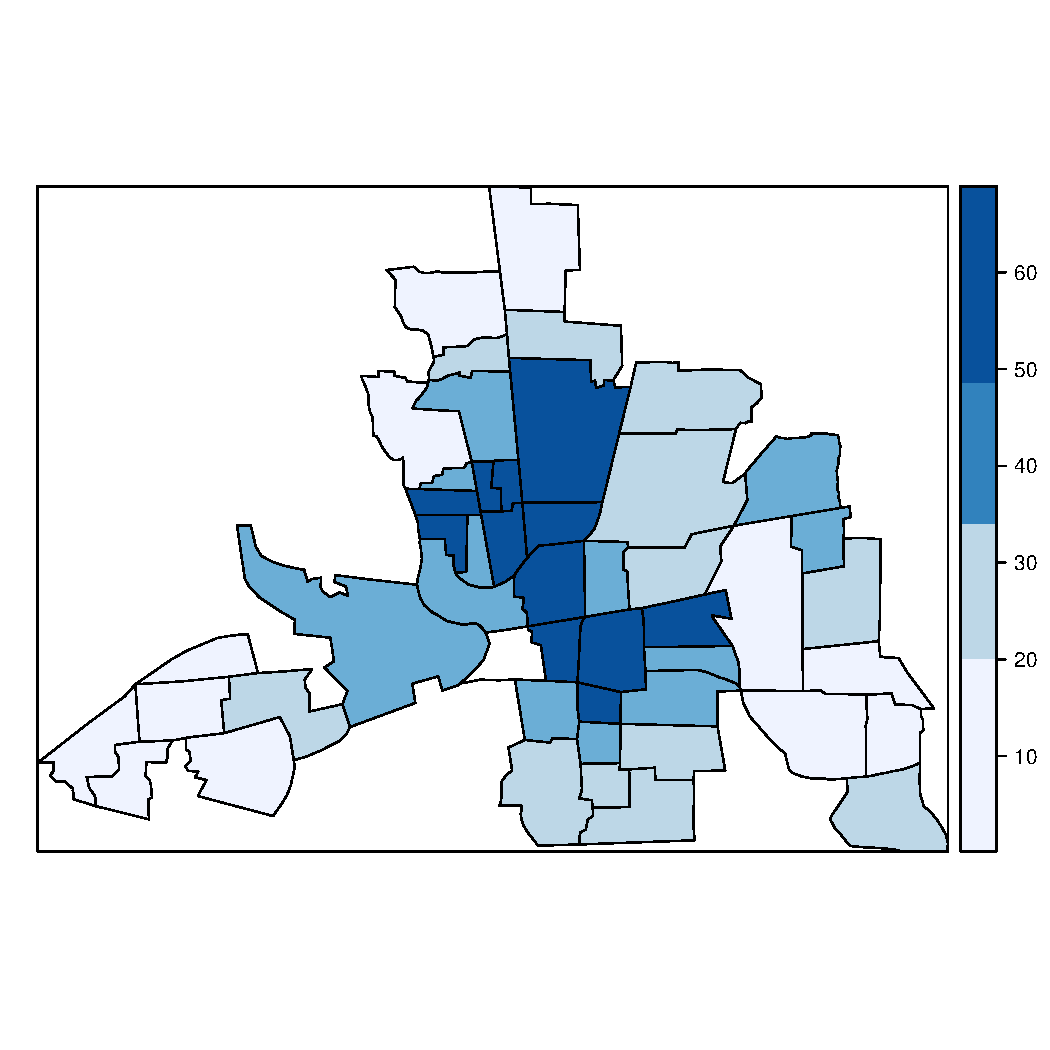
\includegraphics[width=9cm,height=9cm]{figure/spatial-crime-1} 

}


\end{knitrout}
\footnotesize
		\emph{Notes:} This graph shows the spatial distribution of crime on the 49 Columbus, Ohio neighborhoods. Darker color indicates greater rate of crime. 
	\end{minipage}	
\end{figure}


\begin{knitrout}
\definecolor{shadecolor}{rgb}{0.969, 0.969, 0.969}\color{fgcolor}\begin{kframe}
\begin{alltt}
\hlcom{# Moran's I test}
\hlkwd{set.seed}\hlstd{(}\hlnum{1234}\hlstd{)}
\hlstd{listw} \hlkwb{<-} \hlkwd{nb2listw}\hlstd{(col.gal.nb,} \hlkwc{style} \hlstd{=} \hlstr{"W"}\hlstd{)}
\hlkwd{moran.mc}\hlstd{(columbus}\hlopt{$}\hlstd{CRIME,} \hlkwc{listw} \hlstd{= listw,}
           \hlkwc{nsim} \hlstd{=} \hlnum{99}\hlstd{,} \hlkwc{alternative} \hlstd{=} \hlstr{'greater'}\hlstd{)}
\end{alltt}
\begin{verbatim}
## 
## 	Monte-Carlo simulation of Moran I
## 
## data:  columbus$CRIME 
## weights: listw  
## number of simulations + 1: 100 
## 
## statistic = 0.48577, observed rank = 100, p-value = 0.01
## alternative hypothesis: greater
\end{verbatim}
\end{kframe}
\end{knitrout}

The results show that the Moran's I statistic is 0.51 and the p-value is 0.01. This implies that we reject the null hypothesis of random spatial distribution and there exists evidence of positive global spatial autocorrelation in the crime variable: places with high (low) crime rate are surrounded by places with high (low) crime rate. 

Our next step is to estimate different spatial models using the functions already programmed in \pkg{spatialreg}. First, we estimate the classical OLS model followed by the SLX, SLM, SDM, SEM and SAC models. The functions used for each models are the following:

\begin{itemize}
  \item OLS: \code{lm} function.
  \item SLX: \code{lm} function, where $\mW\mX$ is constructed using the function \code{lag.listw} from \pkg{spdep} package. This model can also be estimated using the function \code{lmSLX} from \pkg{spatialreg} package as shown below. 
  \item SLM: \code{lagsarlm} from \pkg{spatialreg} package.  
  \item SDM: \code{lagsarlm} from \pkg{spatialreg} package, using the argument \code{type = "mixed"}. Note that \code{type = "Durbin"} may be used instead of \code{type = "mixed"}. 
  \item SEM: \code{errorsarlm} from \pkg{spatialreg} package. Note that the Spatial Durbin Error Model (SDEM)---not shown here--- can be estimated by using  \code{type = "emixed"}. 
  \item SAC: \code{sacsarlm} from \pkg{spatialreg} package.
\end{itemize}

All models are estimated using ML procedure outline in the previous section. In order to compute the determinant of the Jacobian we use the \cite{ord1975estimation}'s procedure by explicitly using the argument \code{method = "eigen"} in each spatial model. That is, the Jacobian is computed as in (\ref{eq:Ord-determinant}).

\begin{knitrout}
\definecolor{shadecolor}{rgb}{0.969, 0.969, 0.969}\color{fgcolor}\begin{kframe}
\begin{alltt}
\hlcom{# Models}
\hlstd{columbus}\hlopt{$}\hlstd{lag.INC}   \hlkwb{<-} \hlkwd{lag.listw}\hlstd{(listw,}
                         \hlstd{columbus}\hlopt{$}\hlstd{INC)}   \hlcom{# Create spatial lag of INC}
\hlstd{columbus}\hlopt{$}\hlstd{lag.HOVAL} \hlkwb{<-} \hlkwd{lag.listw}\hlstd{(listw,}
                         \hlstd{columbus}\hlopt{$}\hlstd{HOVAL)} \hlcom{# Create spatial lag of HOVAL}
\hlstd{ols} \hlkwb{<-} \hlkwd{lm}\hlstd{(CRIME} \hlopt{~} \hlstd{INC} \hlopt{+} \hlstd{HOVAL,}
          \hlkwc{data} \hlstd{=  columbus)}
\hlstd{slx} \hlkwb{<-} \hlkwd{lm}\hlstd{(CRIME} \hlopt{~} \hlstd{INC} \hlopt{+} \hlstd{HOVAL} \hlopt{+} \hlstd{lag.INC} \hlopt{+} \hlstd{lag.HOVAL,}
          \hlkwc{data} \hlstd{=  columbus)}
\hlstd{slm} \hlkwb{<-} \hlkwd{lagsarlm}\hlstd{(CRIME} \hlopt{~} \hlstd{INC} \hlopt{+} \hlstd{HOVAL,}
                \hlkwc{data} \hlstd{= columbus,}
                \hlstd{listw,}
                \hlkwc{method} \hlstd{=} \hlstr{"eigen"}\hlstd{)}
\hlstd{sdm} \hlkwb{<-} \hlkwd{lagsarlm}\hlstd{(CRIME} \hlopt{~} \hlstd{INC} \hlopt{+} \hlstd{HOVAL,}
                \hlkwc{data} \hlstd{= columbus,}
                \hlstd{listw,}
                \hlkwc{method} \hlstd{=} \hlstr{"eigen"}\hlstd{,}
                \hlkwc{type} \hlstd{=} \hlstr{"mixed"}\hlstd{)}
\hlstd{sem} \hlkwb{<-} \hlkwd{errorsarlm}\hlstd{(CRIME} \hlopt{~} \hlstd{INC} \hlopt{+} \hlstd{HOVAL,}
                \hlkwc{data} \hlstd{= columbus,}
                \hlstd{listw,}
                \hlkwc{method} \hlstd{=} \hlstr{"eigen"}\hlstd{)}
\hlstd{sac} \hlkwb{<-} \hlkwd{sacsarlm}\hlstd{(CRIME} \hlopt{~} \hlstd{INC} \hlopt{+} \hlstd{HOVAL,}
                \hlkwc{data} \hlstd{= columbus,}
                \hlstd{listw,}
                \hlkwc{method} \hlstd{=} \hlstr{"eigen"}\hlstd{)}
\end{alltt}
\end{kframe}
\end{knitrout}

Note that the SLX model can also be estimated as follows:

\begin{knitrout}
\definecolor{shadecolor}{rgb}{0.969, 0.969, 0.969}\color{fgcolor}\begin{kframe}
\begin{alltt}
\hlstd{slx2} \hlkwb{<-} \hlkwd{lmSLX}\hlstd{(CRIME} \hlopt{~} \hlstd{INC} \hlopt{+} \hlstd{HOVAL,}
              \hlkwc{data} \hlstd{= columbus,}
              \hlstd{listw)}
\hlkwd{summary}\hlstd{(slx2)}
\end{alltt}
\end{kframe}
\end{knitrout}



The models are presented in Table \ref{tab:columbus-models}. The OLS estimates are presented in the first column. The results show that an increase of one  thousand dollars in the income of the neighborhood is correlated, in average, with a decreased of 1.6 crimes per thousand households. Similarly, an increase of one thousand dollars in the housing value of the neighborhood is correlated, on average, with a decreased of 0.3 crimes per thousand households. Both correlations are statistically significant.\footnote{Note that we refer to correlation since there may still be some sort of endogeneity problem in either of the two variables.} Both results implies that crimes (residential burglaries and vehicle thefts) are lower in richer neighborhoods. 

Column 2 of Table \ref{tab:columbus-models} show the results for the SLX. In particular, the model is given by $\vy = \mX\vbeta + \mW\mX\vgamma + \vepsi$, where $\mW\mX$ is a $49\times 2$ matrix, whose columns correspond to the spatial lag of \code{INC} and \code{HOVAL}. The coefficient for the spatial lag of \code{INC}, \code{W.INC}, is negative and significant. This implies that crime in spatial unit $i$ is correlated with the income in its neighborhood: the higher the income of the neighbors of $i$ the lower the crime in $i$. This result does not, however, hold for the housing value of the neighbors of $i$ which is positive but not statistically different from zero. 

The results for the SLM are shown in column 3. The spatial autoregressive parameter $\rho$ is positive and significant indicating strong spatial autocorrelation. This implies evidence of spillover effects on crime. The coefficients for the other variables in the regression are similar to the OLS results, though smaller in absolute value.

The results for the SDM are presented in column 4. Whereas the estimated $\rho$ parameter is positive and significant, the coefficient of the lagged explanatory variables are not. This indicates that once we have take into account the endogenous interaction effects of crime, the neighbors' factors do not matter in explaining the crime in each location. Moreover, for the spatial lag of income, the wrong sign is obtained, since the common factor hypothesis would imply a positive sign, given a positive estimate for $\rho$ and negative sign for INC. This provide some evidence that an omitted spatial lag may be the main spatial effect, rather than spatial dependence in the error term. 

Column 5 shows the results for the the SEM model which confirm the conclusions from the previous models. It can be noticed that the autoregressive parameter for $\mW\vu$ is positive and significant indicating an important spatial transmission of the random shocks. This result may be explained by the fact of omitting important variables that are spatially correlated. 

The SAC model, presented in column 6, considers both endogenous interactions effects and interactions effects among the error terms. From the results, we observe that the SAC model produces coefficients estimates of $\mW\vy$ and $\mW\vu$ variables that are not significantly different from zero. However, if endogenous interaction effects and interactions effects among the error terms are separated from each other, both coefficients turn out to be significant. This might be explained by the fact that the model is overparametrized, as a result of which the significance levels of all variables tend to go down. 


\begin{table}[ht]
\caption{Spatial Models for Crime in Columbus, Ohio Neighborhoods.}\label{tab:columbus-models}
\centering
\begin{tabular}{lD{.}{.}{3}D{.}{.}{3}D{.}{.}{3}D{.}{.}{3}D{.}{.}{3}D{.}{.}{3}}
\toprule
 & 
\multicolumn{1}{c}{OLS} & 
\multicolumn{1}{c}{SLX} & 
\multicolumn{1}{c}{SLM} & 
\multicolumn{1}{c}{SDM} & 
\multicolumn{1}{c}{SEM} & 
\multicolumn{1}{c}{SAC}\\
\midrule
\emph{Constant} & 68.619^{***} & 74.029^{***} & 46.851^{***} & 45.593^{***} & 61.054^{***} & 49.051^{***}\\
                 & (4.735) & (6.722) & (7.315) & (13.129) & (5.315) & (10.055)\\
INC              & -1.597^{***} & -1.108^{**} & -1.074^{***} & -0.939^{**} & -0.995^{**} & -1.069^{**}\\
                 & (0.334) & (0.375) & (0.311) & (0.338) & (0.337) & (0.333)\\
HOVAL            & -0.274^{*} & -0.295^{**} & -0.270^{**} & -0.300^{***} & -0.308^{***} & -0.283^{**}\\
                 & (0.103) & (0.101) & (0.090) & (0.091) & (0.093) & (0.092)\\
$W.INC$          &  & -1.383^{*} &  & -0.618 &  & \\
                 &  & (0.559) &  & (0.577) &  & \\
$W.HOVAL$        &  & 0.226 &  & 0.267 &  & \\
                 &  & (0.203) &  & (0.184) &  & \\
$\rho$          &  &  & 0.404^{***} & 0.383^{*} &  & 0.353\\
                 &  &  & (0.121) & (0.162) &  & (0.197)\\
$\lambda$       &  &  &  &  & 0.521^{***} & 0.132\\
                 &  &  &  &  & (0.141) & (0.299)\\
\midrule
AIC              & 382.754 & 380.197 & 376.337 & 378.032 & 378.310 & 378.146\\
N                &  49     &  49     &  49     &  49     &  49     &  49    \\
\bottomrule
\multicolumn{7}{p{.7\linewidth}}{Significance: 
              $*** \equiv p < 0{.}001$; 
              $** \equiv p < 0{.}01$; 
              $* \equiv p < 0{.}05$}\\
\end{tabular}

\end{table}

%---------------------------------------------------
\subsection{Estimation of Marginal Effects in R}
%---------------------------------------------------

In this Section we expand our analysis from Section \ref{sec:lesage-example} in the sense that we now integrate the estimation of the marginal effects using a real estimation from \proglang{R}. 

We begin our analysis with the following question: what would happen to crime in all regions if income rose from 13.906 to 14.906 in the 30th region ($\Delta\texttt{INC} = 1$)? Note that we tried to answer a similar question in the commuting-time example from previous chapter. As we did in Section \ref{sec:lesage-example} we can use the reduced-form predictor given by the following formula:

\begin{equation*}
\widehat{\vy} = \E(\vy| \mX, \mW) = (\mI_n - \widehat{\rho}\mW)^{-1}\mX\widehat{\vbeta},
\end{equation*}
% 
and estimate the predicted values pre- and post- the change in the income variable. In the following lines we use the reduced-form predictor and the observed values of the exogenous variables to obtain the predicted values for \code{CRIME}, $\widehat{\vy}^1$,  using the SLM model previously estimated. 
  
\begin{knitrout}
\definecolor{shadecolor}{rgb}{0.969, 0.969, 0.969}\color{fgcolor}\begin{kframe}
\begin{alltt}
\hlcom{# The predicted values}
\hlstd{rho}       \hlkwb{<-} \hlstd{slm}\hlopt{$}\hlstd{rho}                                \hlcom{# Estimated rho from SLM model}
\hlstd{beta_hat}  \hlkwb{<-} \hlkwd{coef}\hlstd{(slm)[}\hlopt{-}\hlnum{1}\hlstd{]}                          \hlcom{# Estimated parameters}
\hlstd{A}         \hlkwb{<-} \hlkwd{invIrW}\hlstd{(listw,} \hlkwc{rho} \hlstd{= rho)}               \hlcom{# (I - rho*W)^\{-1\}}
\hlstd{X}         \hlkwb{<-} \hlkwd{cbind}\hlstd{(}\hlnum{1}\hlstd{, columbus}\hlopt{$}\hlstd{INC, columbus}\hlopt{$}\hlstd{HOVAL)} \hlcom{# Matrix of observed variables}
\hlstd{y_hat_pre} \hlkwb{<-} \hlstd{A} \hlopt \hlkwd{crossprod}\hlstd{(}\hlkwd{t}\hlstd{(X), beta_hat)}        \hlcom{# y hat}
\end{alltt}
\end{kframe}
\end{knitrout}

Next we increase \code{INC} by 1 in spatial unit 30, and calculate the reduced-form predictions, $\widehat{\vy}^2$.

\begin{knitrout}
\definecolor{shadecolor}{rgb}{0.969, 0.969, 0.969}\color{fgcolor}\begin{kframe}
\begin{alltt}
\hlcom{# The post-predicted values}
\hlstd{col_new} \hlkwb{<-} \hlstd{columbus} \hlcom{# copy the data frame}

\hlcom{# Change the income value}
\hlstd{col_new}\hlopt{@}\hlkwc{data}\hlstd{[col_new}\hlopt{@}\hlkwc{data}\hlopt{$}\hlstd{POLYID} \hlopt{==} \hlnum{30}\hlstd{,} \hlstr{"INC"}\hlstd{]} \hlkwb{<-} \hlnum{14.906}

\hlcom{# The predicted values}
\hlstd{X_d}        \hlkwb{<-} \hlkwd{cbind}\hlstd{(}\hlnum{1}\hlstd{, col_new}\hlopt{$}\hlstd{INC, col_new}\hlopt{$}\hlstd{HOVAL)}
\hlstd{y_hat_post} \hlkwb{<-} \hlstd{A} \hlopt \hlkwd{crossprod}\hlstd{(}\hlkwd{t}\hlstd{(X_d), beta_hat)}
\end{alltt}
\end{kframe}
\end{knitrout}

Finally,  we compute the difference between pre- and post-predictions: $\widehat{\vy}^2 - \widehat{\vy}^1$:

\begin{knitrout}
\definecolor{shadecolor}{rgb}{0.969, 0.969, 0.969}\color{fgcolor}\begin{kframe}
\begin{alltt}
\hlcom{# The difference}
\hlstd{delta_y}         \hlkwb{<-} \hlstd{y_hat_post} \hlopt{-} \hlstd{y_hat_pre}
\hlstd{col_new}\hlopt{$}\hlstd{delta_y} \hlkwb{<-} \hlstd{delta_y}

\hlcom{# Show the effects}
\hlkwd{summary}\hlstd{(delta_y)}
\end{alltt}
\begin{verbatim}
##        V1            
##  Min.   :-1.1141241  
##  1st Qu.:-0.0074114  
##  Median :-0.0012172  
##  Mean   :-0.0336341  
##  3rd Qu.:-0.0002604  
##  Max.   :-0.0000081
\end{verbatim}
\begin{alltt}
\hlkwd{sum}\hlstd{(delta_y)}
\end{alltt}
\begin{verbatim}
## [1] -1.648071
\end{verbatim}
\end{kframe}
\end{knitrout}

According to the result from \code{sum(delta\_y)},  the predicted effect of the change would be a decrease of 1.65 in the crime rate, considering both direct and indirect effects. That is, increasing the income in US\$1,000 in region 30th might generate effects that will transmit through the whole system of region resulting in a new equilibrium where the the total crime will reduce in 1.7 crimes per thousand households. 

Sometimes we would like to plot these effects. Suppose we wanted to show those regions that had low and high impact due to the increase in \code{INC}. Let's define ``high impacted regions'' those regions whose crime rate decrease more than 0.05. The following code produces Figure \ref{fig:predicted-effect}. 

\begin{knitrout}
\definecolor{shadecolor}{rgb}{0.969, 0.969, 0.969}\color{fgcolor}\begin{kframe}
\begin{alltt}
\hlcom{# Breaks}
\hlstd{breaks} \hlkwb{<-} \hlkwd{c}\hlstd{(}\hlkwd{min}\hlstd{(col_new}\hlopt{$}\hlstd{delta_y),} \hlopt{-}\hlnum{0.05}\hlstd{,} \hlkwd{max}\hlstd{(col_new}\hlopt{$}\hlstd{delta_y))}
\hlstd{labels} \hlkwb{<-} \hlkwd{c}\hlstd{(}\hlstr{"High-Impacted Regions"}\hlstd{,} \hlstr{"Low-Impacted Regions"}\hlstd{)}
\hlstd{np}     \hlkwb{<-} \hlkwd{findInterval}\hlstd{(col_new}\hlopt{$}\hlstd{delta_y, breaks)}
\hlstd{colors} \hlkwb{<-} \hlkwd{c}\hlstd{(}\hlstr{"red"}\hlstd{,} \hlstr{"blue"}\hlstd{)}

\hlcom{# Draw Map}
\hlkwd{plot}\hlstd{(col_new,} \hlkwc{col} \hlstd{= colors[np])}
\hlkwd{legend}\hlstd{(}\hlstr{"topleft"}\hlstd{,} \hlkwc{legend} \hlstd{= labels,} \hlkwc{fill} \hlstd{= colors,} \hlkwc{bty} \hlstd{=} \hlstr{"n"}\hlstd{)}
\hlkwd{points}\hlstd{(}\hlnum{38.29}\hlstd{,} \hlnum{30.35}\hlstd{,} \hlkwc{pch} \hlstd{=} \hlnum{19}\hlstd{,} \hlkwc{col} \hlstd{=} \hlstr{"black"}\hlstd{,} \hlkwc{cex} \hlstd{=} \hlnum{0.5}\hlstd{)}
\end{alltt}
\end{kframe}
\end{knitrout}


\begin{figure}[ht]
  \caption{Effects of a Change in Region 30: Categorization}
    \label{fig:predicted-effect}
    \centering 
	\begin{minipage}{.9\linewidth}
\begin{knitrout}
\definecolor{shadecolor}{rgb}{0.969, 0.969, 0.969}\color{fgcolor}

{\centering 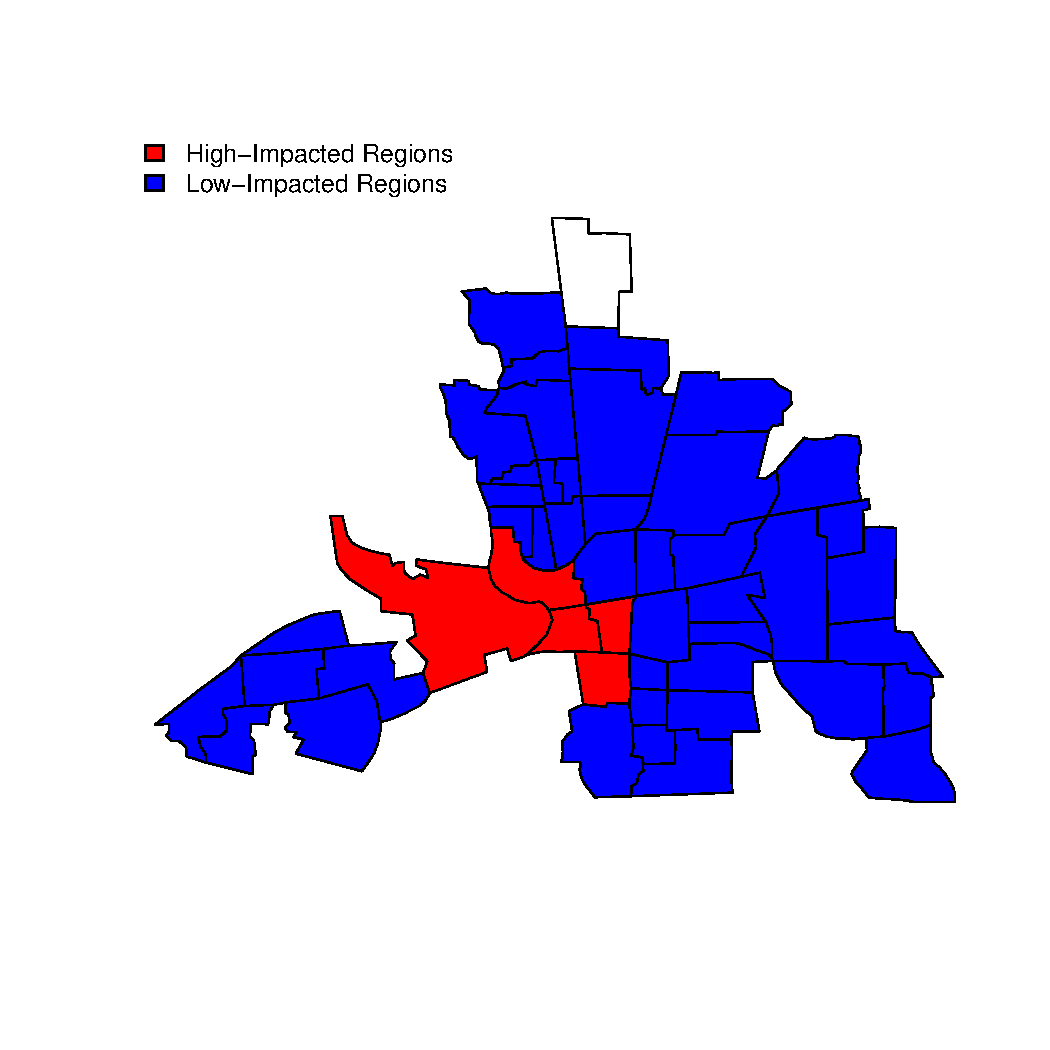
\includegraphics[width=10cm,height=10cm]{figure/predicted-effect-1} 

}


\end{knitrout}
\footnotesize
		\emph{Notes:} This graph shows those regions that had low and high impact due to increase in \code{INC} in 30th. Red-colored regions are those regions with a decrease of crime rate larger than 0.05, whereas blue-colored regions are those regions with lower decrease of crime rate. 
	\end{minipage}	
\end{figure}

Now we map the magnitude of the changes caused by altering \texttt{INC} in region 30. The code is the following and the graph is presented in Figure \ref{fig:predicted-effect2}.

\begin{knitrout}
\definecolor{shadecolor}{rgb}{0.969, 0.969, 0.969}\color{fgcolor}\begin{kframe}
\begin{alltt}
\hlcom{# Plot the magnitude of the ME}
\hlstd{pal5}    \hlkwb{<-} \hlkwd{brewer.pal}\hlstd{(}\hlnum{6}\hlstd{,} \hlstr{"Spectral"}\hlstd{)}
\hlstd{cats5}   \hlkwb{<-} \hlkwd{classIntervals}\hlstd{(col_new}\hlopt{$}\hlstd{delta_y,} \hlkwc{n} \hlstd{=} \hlnum{5}\hlstd{,} \hlkwc{style} \hlstd{=} \hlstr{"jenks"}\hlstd{)}
\hlstd{colors5} \hlkwb{<-} \hlkwd{findColours}\hlstd{(cats5, pal5)}
\hlkwd{plot}\hlstd{(col_new,} \hlkwc{col} \hlstd{= colors5)}
\hlkwd{legend}\hlstd{(}\hlstr{"topleft"}\hlstd{,} \hlkwc{legend} \hlstd{=} \hlkwd{round}\hlstd{(cats5}\hlopt{$}\hlstd{brks,} \hlnum{2}\hlstd{),} \hlkwc{fill} \hlstd{= pal5,} \hlkwc{bty} \hlstd{=} \hlstr{"n"}\hlstd{)}
\end{alltt}
\end{kframe}
\end{knitrout}

\begin{figure}[ht]
  \caption{Effects of a Change in Region 30: Magnitude}
    \label{fig:predicted-effect2}
        \centering 
	\begin{minipage}{.9\linewidth}
\begin{knitrout}
\definecolor{shadecolor}{rgb}{0.969, 0.969, 0.969}\color{fgcolor}

{\centering 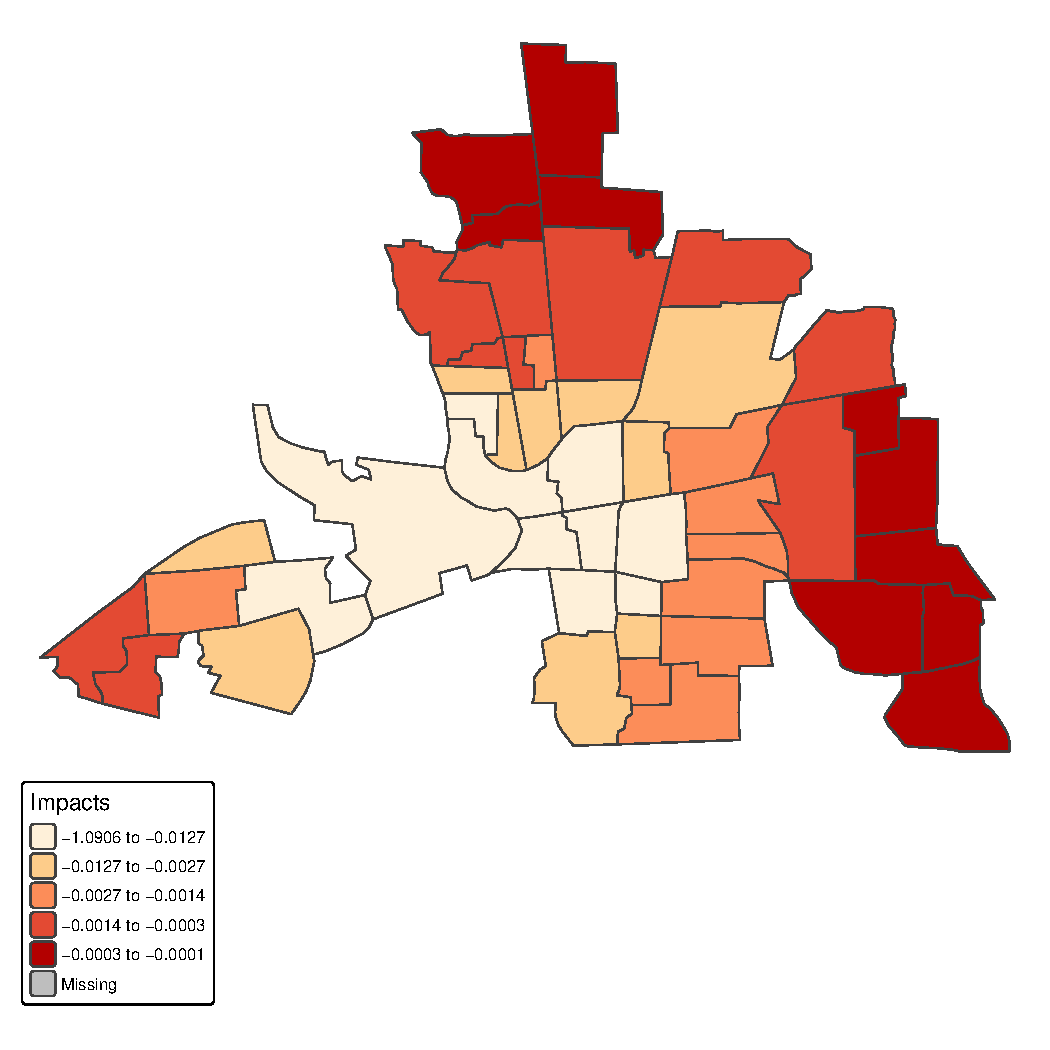
\includegraphics[width=10cm,height=10cm]{figure/predicted-effect2-1} 

}


\end{knitrout}
\footnotesize
		\emph{Notes:} This graph shows the spatial distribution of the changes caused by altering \texttt{INC} in region 30.
	\end{minipage}
\end{figure}


In the rest of this Section we use the \code{impacts()} function from \pkg{spatialreg} package to understand the direct (local), indirect(spillover), and total effect of a unit change in each of the predictor variables. This function returns the direct, indirect and total impacts for the variables in the model. The spatial lag impact measures are computed using the reduced form:

\begin{equation}
  \begin{aligned}
    \vy & = \sum_{r = 1}^K \mA(\mW)^{-1}(\mI_n\beta_r) + \mA(\mW)^{-1}\vepsi \\
     \mA(\mW)^{-1} & = \mI_n + \rho\mW + \rho^2\mW^2 +....
  \end{aligned}
\end{equation}

The exact $\mA(\mW)^{-1}$ is computed when \code{listw} is given. When the traces are created by powering sparse matrices the approximation $\mI_n + \rho\mW + \rho^2\mW^2 +....$ is used. The exact and the trace methods should give very similar results, unless the number of powers used is very small, or the spatial coefficient is close to its bounds. 

\begin{knitrout}
\definecolor{shadecolor}{rgb}{0.969, 0.969, 0.969}\color{fgcolor}\begin{kframe}
\begin{alltt}
\hlkwd{impacts}\hlstd{(slm,} \hlkwc{listw} \hlstd{= listw)}
\end{alltt}
\begin{verbatim}
## Impact measures (lag, exact):
##           Direct   Indirect      Total
## INC   -1.1225156 -0.6783818 -1.8008973
## HOVAL -0.2823163 -0.1706152 -0.4529315
\end{verbatim}
\end{kframe}
\end{knitrout}

The output says that an increase of US\$1,000 in income leads to a decrease of 1.8 crimes per thousand households. 

The direct effect of the income variable in the SLM model amounts to -1.123, while the coefficient estimate of this variable is -1.074. This implies that the feedback effect is -1.123 - (-1.074) = -0.049. This feedback effect corresponds to 4.5\% of the coefficient estimate. 

Let's corroborate these results by computing the impacts using matrix operations:

\begin{knitrout}
\definecolor{shadecolor}{rgb}{0.969, 0.969, 0.969}\color{fgcolor}\begin{kframe}
\begin{alltt}
\hlcom{## Construct S_r(W) = A(W)^-1 (I * beta_r + W * theta_r)}
\hlstd{Ibeta} \hlkwb{<-} \hlkwd{diag}\hlstd{(}\hlkwd{length}\hlstd{(listw}\hlopt{$}\hlstd{neighbours))} \hlopt{*}  \hlkwd{coef}\hlstd{(slm)[}\hlstr{"INC"}\hlstd{]}
\hlstd{S} \hlkwb{<-} \hlstd{A} \hlopt \hlstd{Ibeta}

\hlstd{ADI} \hlkwb{<-} \hlkwd{sum}\hlstd{(}\hlkwd{diag}\hlstd{(S))} \hlopt{/} \hlkwd{nrow}\hlstd{(A)}
\hlstd{ADI}
\end{alltt}
\begin{verbatim}
## [1] -1.122516
\end{verbatim}
\begin{alltt}
\hlstd{n}     \hlkwb{<-} \hlkwd{length}\hlstd{(listw}\hlopt{$}\hlstd{neighbours)}
\hlstd{Total} \hlkwb{<-} \hlkwd{crossprod}\hlstd{(}\hlkwd{rep}\hlstd{(}\hlnum{1}\hlstd{, n), S)} \hlopt \hlkwd{rep}\hlstd{(}\hlnum{1}\hlstd{, n)} \hlopt{/} \hlstd{n}
\hlstd{Total}
\end{alltt}
\begin{verbatim}
##           [,1]
## [1,] -1.800897
\end{verbatim}
\begin{alltt}
\hlstd{Indirect} \hlkwb{<-} \hlstd{Total} \hlopt{-} \hlstd{ADI}
\hlstd{Indirect}
\end{alltt}
\begin{verbatim}
##            [,1]
## [1,] -0.6783818
\end{verbatim}
\end{kframe}
\end{knitrout}

Note that the results are the same as those computed by \code{impact}.

We can also obtain the p-values of the impacts by using the argument $R$. This argument indicates the number of simulations use to create distributions for the impact measures, provided that the fitted model object contains a coefficient covariance matrix. 

Now with p-values:

\begin{knitrout}
\definecolor{shadecolor}{rgb}{0.969, 0.969, 0.969}\color{fgcolor}\begin{kframe}
\begin{alltt}
\hlcom{# Compute standard errors of impacts}
\hlstd{im_obj} \hlkwb{<-} \hlkwd{impacts}\hlstd{(slm,} \hlkwc{listw} \hlstd{= listw,} \hlkwc{R} \hlstd{=} \hlnum{200}\hlstd{)}
\hlkwd{summary}\hlstd{(im_obj,} \hlkwc{zstats} \hlstd{=} \hlnum{TRUE}\hlstd{,} \hlkwc{short} \hlstd{=} \hlnum{TRUE}\hlstd{)}
\end{alltt}
\begin{verbatim}
## Impact measures (lag, exact):
##           Direct   Indirect      Total
## INC   -1.1225156 -0.6783818 -1.8008973
## HOVAL -0.2823163 -0.1706152 -0.4529315
## ========================================================
## Simulation results ( variance matrix):
## ========================================================
## Simulated standard errors
##           Direct  Indirect     Total
## INC   0.28508990 0.3418742 0.5254074
## HOVAL 0.09464442 0.1093738 0.1772125
## 
## Simulated z-values:
##          Direct  Indirect     Total
## INC   -3.857740 -2.090573 -3.453541
## HOVAL -3.114138 -1.761298 -2.750232
## 
## Simulated p-values:
##       Direct     Indirect Total     
## INC   0.00011444 0.036566 0.00055328
## HOVAL 0.00184483 0.078188 0.00595532
\end{verbatim}
\end{kframe}
\end{knitrout}

The results shows that the variable that exerts the largest negative direct impact is \code{INC}. That is, \code{INC} exert the largest reduction on own-crime rate. The indirect effects are presented in the second column. These effects help identify which variables produce the largest spatial spillovers. Negative effects could be considered spatial benefits, since these indicate variables that lead to a reduction in crime rate. Positive indirect effects would represent a negative externality, since this indicates that neighboring regions suffer from an increase in crime rate when these variables increase. From the results we observe that \code{INC} has the largest and significant negative indirect effects. 

The indirect effect for \code{HOVAL} is not significant. The weakly significant effect in the SLM model can be explained by the fact that this model suffers from the problem that the ratio between the spillover effect and the direct effect is the same for every explanatory variable. Therefore, this model is too rigid to model spillover effects adequately. 

Total effect takes into account both the direct and indirect effects, allowing us to draw an inference regarding what variables are important to reduce crime rate. We can observe that \code{INC} has the larges total effect.

Now we follow the example that converts the spatial weight matrix into ``sparse'' matrix, and power it up using the \code{trW} function.

\begin{knitrout}
\definecolor{shadecolor}{rgb}{0.969, 0.969, 0.969}\color{fgcolor}\begin{kframe}
\begin{alltt}
\hlcom{# Impacts using traces. }
\hlstd{W} \hlkwb{<-} \hlkwd{as}\hlstd{(}\hlkwd{nb2listw}\hlstd{(col.gal.nb,} \hlkwc{style} \hlstd{=} \hlstr{"W"}\hlstd{),} \hlstr{"CsparseMatrix"}\hlstd{)}
\hlstd{trMC} \hlkwb{<-} \hlkwd{trW}\hlstd{(W,} \hlkwc{type} \hlstd{=} \hlstr{"MC"}\hlstd{)}
\hlstd{im} \hlkwb{<-} \hlkwd{impacts}\hlstd{(slm,} \hlkwc{tr} \hlstd{= trMC,} \hlkwc{R} \hlstd{=} \hlnum{100}\hlstd{)}
\hlkwd{summary}\hlstd{(im,} \hlkwc{zstats} \hlstd{=}  \hlnum{TRUE}\hlstd{,} \hlkwc{short} \hlstd{=} \hlnum{TRUE}\hlstd{)}
\end{alltt}
\begin{verbatim}
## Impact measures (lag, trace):
##           Direct   Indirect      Total
## INC   -1.1220237 -0.6788736 -1.8008973
## HOVAL -0.2821926 -0.1707389 -0.4529315
## ========================================================
## Simulation results ( variance matrix):
## ========================================================
## Simulated standard errors
##           Direct  Indirect     Total
## INC   0.30303387 0.2985437 0.4706174
## HOVAL 0.09635802 0.1161956 0.1879878
## 
## Simulated z-values:
##          Direct  Indirect     Total
## INC   -3.821767 -2.198798 -3.855705
## HOVAL -2.937362 -1.457964 -2.406792
## 
## Simulated p-values:
##       Direct    Indirect Total    
## INC   0.0001325 0.027892 0.0001154
## HOVAL 0.0033102 0.144850 0.0160933
\end{verbatim}
\end{kframe}
\end{knitrout}


We can also observe the cumulative impacts using the argument \code{Q}. When \code{Q} and \code{tr} are given in the \code{impacts} function the output will present the impact components for each step in the traces of powers of the weight matrix up to and including the $Q$th power. 

\begin{knitrout}
\definecolor{shadecolor}{rgb}{0.969, 0.969, 0.969}\color{fgcolor}\begin{kframe}
\begin{alltt}
\hlcom{# Cumulative impacts}
\hlstd{im2}   \hlkwb{<-} \hlkwd{impacts}\hlstd{(slm,} \hlkwc{tr} \hlstd{= trMC,} \hlkwc{R} \hlstd{=} \hlnum{100}\hlstd{,} \hlkwc{Q} \hlstd{=} \hlnum{5}\hlstd{)}
\hlstd{sums2} \hlkwb{<-} \hlkwd{summary}\hlstd{(im2,} \hlkwc{zstats} \hlstd{=} \hlnum{TRUE}\hlstd{,} \hlkwc{reportQ} \hlstd{=} \hlnum{TRUE}\hlstd{,} \hlkwc{short} \hlstd{=}  \hlnum{TRUE}\hlstd{)}
\hlstd{sums2}
\end{alltt}
\begin{verbatim}
## Impact measures (lag, trace):
##           Direct   Indirect      Total
## INC   -1.1220237 -0.6788736 -1.8008973
## HOVAL -0.2821926 -0.1707389 -0.4529315
## =================================
## Impact components
## $direct
##             INC         HOVAL
## Q1 -1.073533465 -0.2699971236
## Q2  0.000000000  0.0000000000
## Q3 -0.038985415 -0.0098049573
## Q4 -0.005035472 -0.0012664374
## Q5 -0.003072085 -0.0007726393
## 
## $indirect
##            INC        HOVAL
## Q1  0.00000000  0.000000000
## Q2 -0.43358910 -0.109049054
## Q3 -0.13613675 -0.034238831
## Q4 -0.06569456 -0.016522394
## Q5 -0.02549505 -0.006412086
## 
## $total
##            INC        HOVAL
## Q1 -1.07353347 -0.269997124
## Q2 -0.43358910 -0.109049054
## Q3 -0.17512216 -0.044043788
## Q4 -0.07073004 -0.017788832
## Q5 -0.02856713 -0.007184726
## 
## ========================================================
## Simulation results ( variance matrix):
## ========================================================
## Simulated standard errors
##           Direct  Indirect     Total
## INC   0.34631256 0.4029543 0.6401131
## HOVAL 0.08921795 0.1241116 0.1807874
## 
## Simulated z-values:
##          Direct  Indirect     Total
## INC   -3.233305 -1.853701 -2.916189
## HOVAL -3.239503 -1.585160 -2.686904
## 
## Simulated p-values:
##       Direct    Indirect Total    
## INC   0.0012237 0.063782 0.0035434
## HOVAL 0.0011974 0.112930 0.0072118
## ========================================================
## Simulated impact components z-values:
## $Direct
##          INC      HOVAL
## Q1 -3.167835 -3.1796183
## Q2       NaN        NaN
## Q3 -1.703030 -1.5687862
## Q4 -1.272087 -1.0947684
## Q5 -1.002337 -0.8174607
## 
## $Indirect
##          INC      HOVAL
## Q1       NaN        NaN
## Q2 -2.465562 -2.4657025
## Q3 -1.703030 -1.5687862
## Q4 -1.272087 -1.0947684
## Q5 -1.002337 -0.8174607
## 
## $Total
##          INC      HOVAL
## Q1 -3.167835 -3.1796183
## Q2 -2.465562 -2.4657025
## Q3 -1.703030 -1.5687862
## Q4 -1.272087 -1.0947684
## Q5 -1.002337 -0.8174607
## 
## 
## Simulated impact components p-values:
## $Direct
##    INC       HOVAL    
## Q1 0.0015358 0.0014747
## Q2 NA        NA       
## Q3 0.0885624 0.1166978
## Q4 0.2033424 0.2736181
## Q5 0.3161810 0.4136652
## 
## $Indirect
##    INC      HOVAL   
## Q1 NA       NA      
## Q2 0.013680 0.013674
## Q3 0.088562 0.116698
## Q4 0.203342 0.273618
## Q5 0.316181 0.413665
## 
## $Total
##    INC       HOVAL    
## Q1 0.0015358 0.0014747
## Q2 0.0136799 0.0136745
## Q3 0.0885624 0.1166978
## Q4 0.2033424 0.2736181
## Q5 0.3161810 0.4136652
\end{verbatim}
\end{kframe}
\end{knitrout}

%-----------------------------------
\section{Programing the SLM in R}
%-----------------------------------

In this Section, we show how to create our own function to estimate a SLM using ML estimation and two different approaches. First, we create a function to estimate the MLE using a constrained optimization procedure and the log-likelihood function \eqref{eq:LL_SLM_2}. The second approach uses the algorithm outline in Algorithm \eqref{algorithm:SLM}. 

%---------------------------
\subsection{First approach}
%----------------------------

To estimate the SLM using a maximum likelihood procedure, we first create a function that returns the log-likelihood, gradient and Hessian functions. Then, we optimize this function using \code{maxLik} function from \pkg{maxLik} package. 

The following function returns the log-likelihood function: 

\begin{knitrout}
\definecolor{shadecolor}{rgb}{0.969, 0.969, 0.969}\color{fgcolor}\begin{kframe}
\begin{alltt}
\hlcom{# Create log-likelihood function for SLM ----}
\hlstd{sml_ll} \hlkwb{<-} \hlkwa{function}\hlstd{(}\hlkwc{theta}\hlstd{,} \hlkwc{y}\hlstd{,} \hlkwc{X}\hlstd{,} \hlkwc{W}\hlstd{,} \hlkwc{gradient} \hlstd{=} \hlnum{TRUE}\hlstd{,} \hlkwc{hessian} \hlstd{=} \hlnum{TRUE}\hlstd{)\{}
  \hlcom{# Global}
  \hlstd{K} \hlkwb{<-} \hlkwd{ncol}\hlstd{(X)}
  \hlstd{N} \hlkwb{<-} \hlkwd{nrow}\hlstd{(X)}

  \hlcom{# Extract parameters}
  \hlstd{betas}  \hlkwb{<-} \hlstd{theta[}\hlnum{1}\hlopt{:}\hlstd{K]}
  \hlstd{rho}    \hlkwb{<-} \hlstd{theta[K} \hlopt{+} \hlnum{1}\hlstd{]}
  \hlstd{sig.sq} \hlkwb{<-} \hlstd{theta[K} \hlopt{+} \hlnum{2}\hlstd{]}

  \hlcom{# Make residuals}
  \hlstd{A}   \hlkwb{<-} \hlkwd{diag}\hlstd{(N)} \hlopt{-}  \hlstd{rho} \hlopt{*} \hlstd{W}
  \hlstd{Ay}  \hlkwb{<-} \hlstd{A} \hlopt \hlstd{y}
  \hlstd{Xb}  \hlkwb{<-} \hlstd{X} \hlopt \hlstd{betas}
  \hlstd{res} \hlkwb{<-} \hlstd{Ay} \hlopt{-} \hlstd{Xb}

  \hlcom{# Make log-likelihood}
  \hlstd{detA} \hlkwb{<-} \hlkwd{det}\hlstd{(A)}
  \hlstd{ll}   \hlkwb{<-} \hlopt{-}\hlnum{0.5} \hlopt{*} \hlstd{N} \hlopt{*} \hlkwd{log}\hlstd{(}\hlnum{2} \hlopt{*} \hlstd{pi} \hlopt{*} \hlstd{sig.sq)} \hlopt{-} \hlnum{0.5} \hlopt{*} \hlkwd{crossprod}\hlstd{(res)} \hlopt{/} \hlstd{sig.sq} \hlopt{+} \hlkwd{log}\hlstd{(detA)}

  \hlcom{# Gradient}
  \hlkwa{if} \hlstd{(gradient)\{}
    \hlstd{C}           \hlkwb{<-}  \hlstd{W} \hlopt \hlkwd{solve}\hlstd{(A)}
    \hlstd{grad.betas}  \hlkwb{<-} \hlstd{(}\hlnum{1} \hlopt{/} \hlstd{sig.sq)} \hlopt{*} \hlkwd{t}\hlstd{(X)} \hlopt \hlstd{res}
    \hlstd{grad.rho}    \hlkwb{<-} \hlopt{-} \hlkwd{sum}\hlstd{(}\hlkwd{diag}\hlstd{(C))} \hlopt{+} \hlstd{(}\hlnum{1} \hlopt{/} \hlstd{sig.sq)} \hlopt{*} \hlkwd{t}\hlstd{(res)} \hlopt \hlstd{W} \hlopt \hlstd{y}
    \hlstd{grad.sig.sq} \hlkwb{<-} \hlstd{(}\hlnum{1} \hlopt{/} \hlstd{(}\hlnum{2} \hlopt{*} \hlstd{sig.sq} \hlopt{^}\hlnum{2} \hlstd{))} \hlopt{*} \hlstd{(}\hlkwd{t}\hlstd{(res)} \hlopt \hlstd{res} \hlopt{-} \hlstd{N} \hlopt{*} \hlstd{sig.sq)}
    \hlkwd{attr}\hlstd{(ll,} \hlstr{'gradient'}\hlstd{)} \hlkwb{<-} \hlkwd{c}\hlstd{(grad.betas, grad.rho, grad.sig.sq)}
  \hlstd{\}}
  \hlcom{# Hessian}
  \hlkwa{if} \hlstd{(hessian)\{}
    \hlstd{H}    \hlkwb{<-} \hlkwd{matrix}\hlstd{(}\hlnum{NA}\hlstd{,} \hlkwc{nrow} \hlstd{= (K} \hlopt{+} \hlnum{2}\hlstd{),} \hlkwc{ncol} \hlstd{= (K} \hlopt{+} \hlnum{2}\hlstd{))}
    \hlstd{h_bb} \hlkwb{<-} \hlopt{-} \hlstd{(}\hlnum{1} \hlopt{/} \hlstd{sig.sq)} \hlopt{*} \hlkwd{t}\hlstd{(X)} \hlopt \hlstd{X}
    \hlstd{h_bs} \hlkwb{<-} \hlopt{-} \hlstd{(}\hlnum{1} \hlopt{/} \hlstd{sig.sq} \hlopt{^} \hlnum{2}\hlstd{)} \hlopt{*} \hlkwd{t}\hlstd{(X)} \hlopt \hlstd{res}
    \hlstd{h_br} \hlkwb{<-} \hlopt{-} \hlstd{(}\hlnum{1} \hlopt{/} \hlstd{sig.sq)} \hlopt{*} \hlkwd{t}\hlstd{(X)} \hlopt \hlstd{W} \hlopt \hlstd{y}
    \hlstd{h_ss} \hlkwb{<-} \hlstd{(N} \hlopt{/} \hlstd{(}\hlnum{2} \hlopt{*} \hlstd{sig.sq} \hlopt{^} \hlnum{2}\hlstd{))} \hlopt{-} \hlstd{(}\hlnum{1} \hlopt{/} \hlstd{sig.sq} \hlopt{^} \hlnum{3}\hlstd{)} \hlopt{*} \hlkwd{t}\hlstd{(res)} \hlopt \hlstd{res}
    \hlstd{h_sr} \hlkwb{<-}  \hlopt{-} \hlkwd{t}\hlstd{(res)} \hlopt \hlstd{W} \hlopt \hlstd{y} \hlopt{/} \hlstd{sig.sq} \hlopt{^} \hlnum{2}
    \hlstd{h_rr} \hlkwb{<-} \hlopt{-} \hlkwd{sum}\hlstd{(}\hlkwd{diag}\hlstd{(C} \hlopt \hlstd{C))} \hlopt{-} \hlstd{(}\hlnum{1} \hlopt{/} \hlstd{sig.sq)} \hlopt{*} \hlstd{(}\hlkwd{t}\hlstd{(y)} \hlopt \hlkwd{t}\hlstd{(W)} \hlopt \hlstd{W} \hlopt \hlstd{y)}
    \hlstd{H[}\hlnum{1}\hlopt{:}\hlstd{K,} \hlnum{1}\hlopt{:}\hlstd{K]}     \hlkwb{<-} \hlstd{h_bb}
    \hlstd{H[}\hlnum{1}\hlopt{:}\hlstd{K, K} \hlopt{+} \hlnum{1}\hlstd{]}   \hlkwb{<-} \hlstd{h_bs}
    \hlstd{H[}\hlnum{1}\hlopt{:}\hlstd{K, K} \hlopt{+} \hlnum{2}\hlstd{]}   \hlkwb{<-} \hlstd{h_br}
    \hlstd{H[K} \hlopt{+} \hlnum{1}\hlstd{,} \hlnum{1}\hlopt{:}\hlstd{K]}   \hlkwb{<-} \hlkwd{t}\hlstd{(h_bs)}
    \hlstd{H[K} \hlopt{+} \hlnum{1}\hlstd{, K} \hlopt{+} \hlnum{1}\hlstd{]} \hlkwb{<-} \hlstd{h_ss}
    \hlstd{H[K} \hlopt{+} \hlnum{1}\hlstd{, K} \hlopt{+} \hlnum{2}\hlstd{]} \hlkwb{<-} \hlstd{h_sr}
    \hlstd{H[K} \hlopt{+} \hlnum{2}\hlstd{,} \hlnum{1}\hlopt{:}\hlstd{K]}   \hlkwb{<-} \hlkwd{t}\hlstd{(h_br)}
    \hlstd{H[K} \hlopt{+} \hlnum{2}\hlstd{, K} \hlopt{+} \hlnum{1}\hlstd{]} \hlkwb{<-} \hlstd{h_sr}
    \hlstd{H[K} \hlopt{+} \hlnum{2}\hlstd{, K} \hlopt{+} \hlnum{2}\hlstd{]} \hlkwb{<-} \hlstd{h_rr}
    \hlkwd{attr}\hlstd{(ll,} \hlstr{'hessian'}\hlstd{)} \hlkwb{<-} \hlstd{H}
  \hlstd{\}}
  \hlkwd{return}\hlstd{(ll)}
\hlstd{\}}
\end{alltt}
\end{kframe}
\end{knitrout}

The function \code{sml\_ll} has the following arguments: \code{theta} is a $K + 2$ vector of parameters where the $K + 1$ and $K + 2$ elements are $\rho$ and $\sigma^2$, respectively; \code{y} is the $n\times 1$ vector of dependent variables; \code{X} is the $n\times k$ matrix of independent variables; \code{W} is the spatial weight matrix in \code{matrix} class; the arguments \code{gradient} and \code{hessian} indicate whether the analytical gradient and Hessian, respectively, should be use in the numerical optimization algorithm.

The log-likelihood function is given by object \code{ll} in \code{sml\_ll} function. This object is based on Equation \eqref{eq:LL_SLM_2}. The gradient is coded following Equation \eqref{eq:full_agradient}, whereas the Hessian is based on Equation \eqref{eq:hessian_sml}.

The following function estimates the model by ML using a constrained optimization procedure. The optimization is made by \code{maxLik} function:

\begin{knitrout}
\definecolor{shadecolor}{rgb}{0.969, 0.969, 0.969}\color{fgcolor}\begin{kframe}
\begin{alltt}
\hlstd{slm_ml} \hlkwb{<-} \hlkwa{function}\hlstd{(}\hlkwc{formula}\hlstd{,} \hlkwc{data}\hlstd{,} \hlkwc{listw}\hlstd{,}
                   \hlkwc{gradient} \hlstd{=} \hlnum{TRUE}\hlstd{,}
                   \hlkwc{hessian}  \hlstd{=} \hlnum{TRUE}\hlstd{,} \hlkwc{...}\hlstd{)\{}
  \hlkwd{require}\hlstd{(}\hlstr{"maxLik"}\hlstd{)}
  \hlkwd{require}\hlstd{(}\hlstr{"spdep"}\hlstd{)}
  \hlcom{# Model Frame: This part is standard in R to obtain}
  \hlcom{#              the variables using formula and data argument.}
  \hlstd{callT} \hlkwb{<-} \hlkwd{match.call}\hlstd{(}\hlkwc{expand.dots} \hlstd{=} \hlnum{TRUE}\hlstd{)}
  \hlstd{mf} \hlkwb{<-} \hlstd{callT}
  \hlstd{m}  \hlkwb{<-} \hlkwd{match}\hlstd{(}\hlkwd{c}\hlstd{(}\hlstr{"formula"}\hlstd{,} \hlstr{"data"}\hlstd{),} \hlkwd{names}\hlstd{(mf),} \hlnum{0L}\hlstd{)}
  \hlstd{mf} \hlkwb{<-} \hlstd{mf[}\hlkwd{c}\hlstd{(}\hlnum{1L}\hlstd{, m)]}
  \hlstd{mf[[}\hlnum{1L}\hlstd{]]} \hlkwb{<-} \hlkwd{as.name}\hlstd{(}\hlstr{"model.frame"}\hlstd{)}
  \hlstd{mf} \hlkwb{<-} \hlkwd{eval}\hlstd{(mf,} \hlkwd{parent.frame}\hlstd{())} \hlcom{# final model frame}
  \hlstd{nframe}     \hlkwb{<-} \hlkwd{length}\hlstd{(}\hlkwd{sys.calls}\hlstd{())}

  \hlcom{# Get variables and globals}
  \hlstd{y}  \hlkwb{<-} \hlkwd{model.response}\hlstd{(mf)}        \hlcom{# Get dependent variable from mf}
  \hlstd{X}  \hlkwb{<-} \hlkwd{model.matrix}\hlstd{(formula, mf)} \hlcom{# Get X from mf}
  \hlstd{W}  \hlkwb{<-} \hlkwd{listw2mat}\hlstd{(listw)}          \hlcom{# listw to matrix}
  \hlstd{K}  \hlkwb{<-} \hlkwd{ncol}\hlstd{(X)}

  \hlcom{# Starting values}
  \hlstd{b_hat} \hlkwb{<-} \hlkwd{coef}\hlstd{(}\hlkwd{lm}\hlstd{(y} \hlopt{~} \hlstd{X} \hlopt{-} \hlnum{1}\hlstd{))}
  \hlstd{start} \hlkwb{<-} \hlkwd{c}\hlstd{(b_hat,} \hlnum{0}\hlstd{,} \hlnum{1}\hlstd{)}
  \hlkwd{names}\hlstd{(start)} \hlkwb{<-} \hlkwd{c}\hlstd{(}\hlkwd{colnames}\hlstd{(X),} \hlstr{"rho"}\hlstd{,} \hlstr{"sig.sq"}\hlstd{)}

  \hlcom{# Restricted optimization: A %*% theta + B >= 0: Constraint rho and sigma2}
  \hlstd{sym}          \hlkwb{<-} \hlkwd{all}\hlstd{(W} \hlopt{==} \hlkwd{t}\hlstd{(W))}
  \hlstd{omega}        \hlkwb{<-} \hlkwd{eigen}\hlstd{(W,} \hlkwc{only.values} \hlstd{=} \hlnum{TRUE}\hlstd{,} \hlkwc{symmetric} \hlstd{= sym)}
  \hlstd{lambda_space} \hlkwb{<-} \hlkwa{if} \hlstd{(}\hlkwd{is.complex}\hlstd{(omega}\hlopt{$}\hlstd{values))} \hlnum{1} \hlopt{/} \hlkwd{range}\hlstd{(}\hlkwd{Re}\hlstd{(omega}\hlopt{$}\hlstd{values))} \hlkwa{else} \hlnum{1} \hlopt{/} \hlkwd{range}\hlstd{(omega}\hlopt{$}\hlstd{values)}

  \hlstd{A} \hlkwb{<-} \hlkwd{rbind}\hlstd{(}\hlkwd{c}\hlstd{(}\hlkwd{rep}\hlstd{(}\hlnum{0}\hlstd{, K),} \hlnum{1}\hlstd{,} \hlnum{0}\hlstd{),}
             \hlkwd{c}\hlstd{(}\hlkwd{rep}\hlstd{(}\hlnum{0}\hlstd{, K),} \hlopt{-}\hlnum{1}\hlstd{,} \hlnum{0}\hlstd{),}
             \hlkwd{c}\hlstd{(}\hlkwd{rep}\hlstd{(}\hlnum{0}\hlstd{, K),} \hlnum{0}\hlstd{,} \hlnum{1}\hlstd{))}
  \hlstd{B} \hlkwb{<-} \hlkwd{c}\hlstd{(}\hlopt{-}\hlnum{1L} \hlopt{*} \hlstd{(lambda_space[}\hlnum{1}\hlstd{]} \hlopt{+} \hlkwd{sqrt}\hlstd{(.Machine}\hlopt{$}\hlstd{double.eps)),}
                \hlstd{lambda_space[}\hlnum{2}\hlstd{]} \hlopt{-} \hlkwd{sqrt}\hlstd{(.Machine}\hlopt{$}\hlstd{double.eps),}
         \hlopt{-}\hlnum{1L}\hlopt{*} \hlkwd{sqrt}\hlstd{(.Machine}\hlopt{$}\hlstd{double.eps))}
  \hlstd{callT}\hlopt{$}\hlstd{constraints} \hlkwb{<-} \hlkwd{list}\hlstd{(}\hlkwc{ineqA} \hlstd{= A,} \hlkwc{ineqB} \hlstd{= B)}

  \hlcom{# Optimization default controls if not added by user}
  \hlkwa{if} \hlstd{(}\hlkwd{is.null}\hlstd{(callT}\hlopt{$}\hlstd{method))  callT}\hlopt{$}\hlstd{method}  \hlkwb{<-} \hlstr{'bfgs'}
  \hlkwa{if} \hlstd{(}\hlkwd{is.null}\hlstd{(callT}\hlopt{$}\hlstd{iterlim)) callT}\hlopt{$}\hlstd{iterlim} \hlkwb{<-} \hlnum{100000}
  \hlstd{opt} \hlkwb{<-} \hlstd{callT}
  \hlstd{m} \hlkwb{<-} \hlkwd{match}\hlstd{(}\hlkwd{c}\hlstd{(}\hlstr{'method'}\hlstd{,} \hlstr{'print.level'}\hlstd{,} \hlstr{'iterlim'}\hlstd{,}
               \hlstr{'tol'}\hlstd{,} \hlstr{'ftol'}\hlstd{,} \hlstr{'steptol'}\hlstd{,} \hlstr{'fixed'}\hlstd{,} \hlstr{'constraints'}\hlstd{,}
               \hlstr{'control'}\hlstd{,} \hlstr{'finalHessian'}\hlstd{,} \hlstr{'reltol'}\hlstd{,} \hlstr{'rho'}\hlstd{,} \hlstr{'outer.iterations'}\hlstd{,} \hlstr{'outer.eps'}\hlstd{),}
             \hlkwd{names}\hlstd{(opt),} \hlnum{0L}\hlstd{)}
  \hlstd{opt} \hlkwb{<-} \hlstd{opt[}\hlkwd{c}\hlstd{(}\hlnum{1L}\hlstd{, m)]}
  \hlstd{opt}\hlopt{$}\hlstd{start}     \hlkwb{<-} \hlstd{start}
  \hlstd{opt[[}\hlnum{1}\hlstd{]]}      \hlkwb{<-} \hlkwd{as.name}\hlstd{(}\hlstr{'maxLik'}\hlstd{)}
  \hlstd{opt}\hlopt{$}\hlstd{logLik}    \hlkwb{<-} \hlkwd{as.name}\hlstd{(}\hlstr{'sml_ll'}\hlstd{)}
  \hlstd{opt}\hlopt{$}\hlstd{gradient}  \hlkwb{<-} \hlstd{gradient}
  \hlstd{opt}\hlopt{$}\hlstd{hessian}   \hlkwb{<-} \hlstd{hessian}
  \hlstd{opt[}\hlkwd{c}\hlstd{(}\hlstr{'y'}\hlstd{,} \hlstr{'W'}\hlstd{,} \hlstr{'X'}\hlstd{)]} \hlkwb{<-} \hlkwd{list}\hlstd{(}\hlkwd{as.name}\hlstd{(}\hlstr{'y'}\hlstd{),}
                                \hlkwd{as.name}\hlstd{(}\hlstr{'W'}\hlstd{),}
                                \hlkwd{as.name}\hlstd{(}\hlstr{'X'}\hlstd{))}
  \hlstd{out} \hlkwb{<-} \hlkwd{eval}\hlstd{(opt,} \hlkwd{sys.frame}\hlstd{(}\hlkwc{which} \hlstd{= nframe))}
  \hlkwd{return}\hlstd{(out)}
\hlstd{\}}
\end{alltt}
\end{kframe}
\end{knitrout}

Now, we use our function:

\begin{knitrout}
\definecolor{shadecolor}{rgb}{0.969, 0.969, 0.969}\color{fgcolor}\begin{kframe}
\begin{alltt}
\hlcom{# Load data }
\hlkwd{data}\hlstd{(oldcol,} \hlkwc{package}\hlstd{=}\hlstr{"spdep"}\hlstd{)}
\hlstd{listw} \hlkwb{<-} \hlstd{spdep}\hlopt{::}\hlkwd{nb2listw}\hlstd{(COL.nb,} \hlkwc{style} \hlstd{=} \hlstr{"W"}\hlstd{)}

\hlcom{# Use our function }
\hlstd{test1} \hlkwb{<-} \hlkwd{slm_ml}\hlstd{(CRIME} \hlopt{~} \hlstd{INC} \hlopt{+} \hlstd{HOVAL,} \hlkwc{data} \hlstd{= COL.OLD,} \hlkwc{listw} \hlstd{= listw)}
\hlkwd{summary}\hlstd{(test1)}
\end{alltt}
\begin{verbatim}
## --------------------------------------------
## Maximum Likelihood estimation
## BFGS maximization, 124 iterations
## Return code 0: successful convergence 
## Log-Likelihood: -182.3918 
## 5  free parameters
## Estimates:
##             Estimate Std. error t value  Pr(> t)    
## (Intercept) 44.87928    7.83040   5.731 9.96e-09 ***
## INC         -1.02620    0.32675  -3.141  0.00169 ** 
## HOVAL       -0.26550    0.08778  -3.025  0.00249 ** 
## rho          0.43394   19.12486   0.023  0.98190    
## sig.sq      94.54494    0.12299 768.723  < 2e-16 ***
## ---
## Signif. codes:  0 '***' 0.001 '**' 0.01 '*' 0.05 '.' 0.1 ' ' 1
## 
## Warning: constrained likelihood estimation. Inference is probably wrong
## Constrained optimization based on constrOptim 
## 1  outer iterations, barrier value -0.008952326 
## --------------------------------------------
\end{verbatim}
\begin{alltt}
\hlcom{# Use lagsarlm from spatialreg}
\hlkwd{library}\hlstd{(}\hlstr{"spatialreg"}\hlstd{)}
\hlstd{sreg} \hlkwb{<-} \hlkwd{lagsarlm}\hlstd{(CRIME} \hlopt{~} \hlstd{INC} \hlopt{+} \hlstd{HOVAL,} \hlkwc{data} \hlstd{= COL.OLD,} \hlkwc{listw} \hlstd{= listw)}
\hlkwd{summary}\hlstd{(sreg)}
\end{alltt}
\begin{verbatim}
## 
## Call:lagsarlm(formula = CRIME ~ INC + HOVAL, data = COL.OLD, listw = listw)
## 
## Residuals:
##       Min        1Q    Median        3Q       Max 
## -37.68585  -5.35636   0.05421   6.02013  23.20555 
## 
## Type: lag 
## Coefficients: (asymptotic standard errors) 
##              Estimate Std. Error z value  Pr(>|z|)
## (Intercept) 45.079251   7.177347  6.2808 3.369e-10
## INC         -1.031616   0.305143 -3.3808 0.0007229
## HOVAL       -0.265926   0.088499 -3.0049 0.0026570
## 
## Rho: 0.43102, LR test value: 9.9736, p-value: 0.001588
## Asymptotic standard error: 0.11768
##     z-value: 3.6626, p-value: 0.00024962
## Wald statistic: 13.415, p-value: 0.00024962
## 
## Log likelihood: -182.3904 for lag model
## ML residual variance (sigma squared): 95.494, (sigma: 9.7721)
## Number of observations: 49 
## Number of parameters estimated: 5 
## AIC: 374.78, (AIC for lm: 382.75)
## LM test for residual autocorrelation
## test value: 0.31955, p-value: 0.57188
\end{verbatim}
\end{kframe}
\end{knitrout}

%---------------------------
\subsection{Second approach}
%----------------------------

Now, we create a function that estimates the parameters of the SLM using the steps in  Algorithm \eqref{algorithm:SLM}.

\begin{knitrout}
\definecolor{shadecolor}{rgb}{0.969, 0.969, 0.969}\color{fgcolor}\begin{kframe}
\begin{alltt}
\hlstd{logLik_sar} \hlkwb{<-} \hlkwa{function}\hlstd{(}\hlkwc{rho}\hlstd{,} \hlkwc{e_0}\hlstd{,} \hlkwc{e_L}\hlstd{,} \hlkwc{omega}\hlstd{,} \hlkwc{n}\hlstd{)}
\hlstd{\{}
  \hlcom{# This function returns the concentrated log L for maximization}

  \hlcom{#Generate determinant using Ord's approximation}
  \hlstd{det}    \hlkwb{<-} \hlkwa{if} \hlstd{(}\hlkwd{is.complex}\hlstd{(omega))} \hlkwd{Re}\hlstd{(}\hlkwd{prod}\hlstd{(}\hlnum{1} \hlopt{-} \hlstd{rho} \hlopt{*} \hlstd{omega))} \hlkwa{else} \hlkwd{prod}\hlstd{(}\hlnum{1} \hlopt{-} \hlstd{rho} \hlopt{*} \hlstd{omega)}
  \hlstd{e_diff} \hlkwb{<-} \hlstd{e_0} \hlopt{-} \hlstd{rho} \hlopt{*} \hlstd{e_L}
  \hlstd{sigma2} \hlkwb{<-} \hlkwd{crossprod}\hlstd{(e_diff)} \hlopt{/} \hlstd{n}

  \hlcom{#Log-Likelihood function}
  \hlstd{l_c}    \hlkwb{<-} \hlopt{-} \hlstd{(n} \hlopt{/} \hlnum{2}\hlstd{)} \hlopt{-} \hlstd{(n} \hlopt{/} \hlnum{2}\hlstd{)} \hlopt{*} \hlkwd{log}\hlstd{(}\hlnum{2} \hlopt{*} \hlstd{pi)} \hlopt{-} \hlstd{(n} \hlopt{/} \hlnum{2}\hlstd{)} \hlopt{*} \hlkwd{log}\hlstd{(sigma2)} \hlopt{+} \hlkwd{log}\hlstd{(det)}
  \hlkwd{return}\hlstd{(l_c)}
\hlstd{\}}
\end{alltt}
\end{kframe}
\end{knitrout}

\begin{knitrout}
\definecolor{shadecolor}{rgb}{0.969, 0.969, 0.969}\color{fgcolor}\begin{kframe}
\begin{alltt}
\hlstd{sarML} \hlkwb{<-} \hlkwa{function}\hlstd{(}\hlkwc{formula}\hlstd{,} \hlkwc{data}\hlstd{,} \hlkwc{listw}\hlstd{)}
\hlstd{\{}
  \hlkwd{require}\hlstd{(}\hlstr{"spdep"}\hlstd{)}
  \hlcom{# Model Frame: This part is standard in R to obtain}
  \hlcom{# the variables using formula and data argument.}
  \hlstd{callT} \hlkwb{<-} \hlkwd{match.call}\hlstd{(}\hlkwc{expand.dots} \hlstd{=} \hlnum{TRUE}\hlstd{)}
  \hlstd{mf} \hlkwb{<-} \hlstd{callT}
  \hlstd{m}  \hlkwb{<-} \hlkwd{match}\hlstd{(}\hlkwd{c}\hlstd{(}\hlstr{"formula"}\hlstd{,} \hlstr{"data"}\hlstd{),} \hlkwd{names}\hlstd{(mf),} \hlnum{0L}\hlstd{)}
  \hlstd{mf} \hlkwb{<-} \hlstd{mf[}\hlkwd{c}\hlstd{(}\hlnum{1L}\hlstd{, m)]}
  \hlstd{mf[[}\hlnum{1L}\hlstd{]]} \hlkwb{<-} \hlkwd{as.name}\hlstd{(}\hlstr{"model.frame"}\hlstd{)}
  \hlstd{mf} \hlkwb{<-} \hlkwd{eval}\hlstd{(mf,} \hlkwd{parent.frame}\hlstd{())} \hlcom{# final model frame}

  \hlcom{# Get variables and Globals}
  \hlstd{y}  \hlkwb{<-} \hlkwd{model.response}\hlstd{(mf)}        \hlcom{# Get dependent variable from mf}
  \hlstd{X}  \hlkwb{<-} \hlkwd{model.matrix}\hlstd{(formula, mf)} \hlcom{# Get X from mf}
  \hlstd{n}  \hlkwb{<-} \hlkwd{nrow}\hlstd{(X)}                   \hlcom{# Number of spatial units}
  \hlstd{k}  \hlkwb{<-} \hlkwd{ncol}\hlstd{(X)}                   \hlcom{# Number of regressors}
  \hlstd{Wy} \hlkwb{<-} \hlkwd{lag.listw}\hlstd{(listw, y)}       \hlcom{# Spatial lag}
  \hlstd{W}  \hlkwb{<-} \hlkwd{listw2mat}\hlstd{(listw)}          \hlcom{# listw to matrix}

  \hlcom{# Generate auxiliary regressions }
  \hlcom{# See Algorithm 3.1}
  \hlstd{ols_0} \hlkwb{<-} \hlkwd{lm}\hlstd{(y} \hlopt{~} \hlstd{X} \hlopt{-} \hlnum{1}\hlstd{)}
  \hlstd{ols_L} \hlkwb{<-} \hlkwd{lm}\hlstd{(Wy} \hlopt{~} \hlstd{X} \hlopt{-} \hlnum{1}\hlstd{)}
  \hlstd{e_0}   \hlkwb{<-} \hlkwd{residuals}\hlstd{(ols_0)}
  \hlstd{e_L}   \hlkwb{<-} \hlkwd{residuals}\hlstd{(ols_L)}

  \hlcom{# Get eigenvalues to constraint the optimization}
  \hlstd{omega} \hlkwb{<-} \hlkwd{eigenw}\hlstd{(listw)}

  \hlcom{# Maximize concentrated log-likelihood}
  \hlstd{rho_space} \hlkwb{<-} \hlkwa{if} \hlstd{(}\hlkwd{is.complex}\hlstd{(omega))} \hlnum{1} \hlopt{/} \hlkwd{range}\hlstd{(}\hlkwd{Re}\hlstd{(eig))} \hlkwa{else} \hlnum{1} \hlopt{/} \hlkwd{range}\hlstd{(omega)}
  \hlstd{opt_lc} \hlkwb{<-} \hlkwd{optimize}\hlstd{(}\hlkwc{f} \hlstd{= logLik_sar,}   \hlcom{# This function is below}
                     \hlkwc{lower} \hlstd{= rho_space[}\hlnum{1}\hlstd{]} \hlopt{+} \hlstd{.Machine}\hlopt{$}\hlstd{double.eps,}
                     \hlkwc{upper} \hlstd{= rho_space[}\hlnum{2}\hlstd{]} \hlopt{-} \hlstd{.Machine}\hlopt{$}\hlstd{double.eps,}
                     \hlkwc{maximum} \hlstd{=} \hlnum{TRUE}\hlstd{,}
                     \hlkwc{e_0} \hlstd{= e_0,} \hlkwc{e_L} \hlstd{= e_L,} \hlkwc{omega} \hlstd{= omega,} \hlkwc{n} \hlstd{= n)}
  \hlcom{# Obtain rho_hat from concentrated log-likelihood}
  \hlstd{rho_hat} \hlkwb{<-} \hlstd{opt_lc}\hlopt{$}\hlstd{maximum}

  \hlcom{# Generate estimates}
  \hlstd{A}          \hlkwb{<-} \hlstd{(}\hlkwd{diag}\hlstd{(n)} \hlopt{-} \hlstd{rho_hat} \hlopt{*} \hlstd{W)}
  \hlstd{Ay}         \hlkwb{<-} \hlkwd{crossprod}\hlstd{(}\hlkwd{t}\hlstd{(A), y)}
  \hlstd{beta_hat}   \hlkwb{<-} \hlkwd{solve}\hlstd{(}\hlkwd{crossprod}\hlstd{(X))} \hlopt \hlkwd{crossprod}\hlstd{(X, Ay)} \hlcom{# See Equation (3.25)}
  \hlstd{error}      \hlkwb{<-} \hlstd{Ay} \hlopt{-} \hlkwd{crossprod}\hlstd{(}\hlkwd{t}\hlstd{(X), beta_hat)}
  \hlstd{sigma2_hat} \hlkwb{<-} \hlkwd{crossprod}\hlstd{(error)} \hlopt{/} \hlstd{n}                     \hlcom{# See Equation (3.26)}

  \hlcom{# Hessian}
  \hlstd{C}       \hlkwb{<-} \hlkwd{crossprod}\hlstd{(}\hlkwd{t}\hlstd{(W),} \hlkwd{solve}\hlstd{(A))} \hlcom{# C = WA^\{-1\}}
  \hlstd{alpha}   \hlkwb{<-}  \hlkwd{sum}\hlstd{(omega} \hlopt{^} \hlnum{2} \hlopt{/} \hlstd{((}\hlnum{1} \hlopt{-} \hlstd{rho_hat} \hlopt{*} \hlstd{omega)} \hlopt{^} \hlnum{2}\hlstd{))}
  \hlkwa{if} \hlstd{(}\hlkwd{is.complex}\hlstd{(alpha)) alpha} \hlkwb{<-} \hlkwd{Re}\hlstd{(alpha)}
  \hlstd{b_b}     \hlkwb{<-} \hlkwd{drop}\hlstd{(}\hlnum{1} \hlopt{/} \hlstd{sigma2_hat)} \hlopt{*} \hlkwd{crossprod}\hlstd{(X)} \hlcom{# k * k}
  \hlstd{b_rho}   \hlkwb{<-} \hlkwd{drop}\hlstd{(}\hlnum{1} \hlopt{/} \hlstd{sigma2_hat)} \hlopt{*} \hlstd{(}\hlkwd{t}\hlstd{(X)} \hlopt \hlstd{C} \hlopt \hlstd{X} \hlopt \hlstd{beta_hat)} \hlcom{# k * 1}
  \hlstd{sig_sig} \hlkwb{<-} \hlstd{n} \hlopt{/} \hlstd{(}\hlnum{2} \hlopt{*} \hlstd{sigma2_hat} \hlopt{^} \hlnum{2}\hlstd{)} \hlcom{# 1 * 1}
  \hlstd{sig_rho} \hlkwb{<-} \hlkwd{drop}\hlstd{(}\hlnum{1} \hlopt{/} \hlstd{sigma2_hat)} \hlopt{*} \hlkwd{sum}\hlstd{(}\hlkwd{diag}\hlstd{(C))} \hlcom{# 1 * 1}
  \hlstd{rho_rho} \hlkwb{<-} \hlkwd{sum}\hlstd{(}\hlkwd{diag}\hlstd{(}\hlkwd{crossprod}\hlstd{(C)))} \hlopt{+}  \hlstd{alpha} \hlopt{+}
    \hlkwd{drop}\hlstd{(}\hlnum{1} \hlopt{/} \hlstd{sigma2_hat)} \hlopt{*} \hlkwd{crossprod}\hlstd{(C} \hlopt \hlstd{X} \hlopt \hlstd{beta_hat)} \hlcom{# 1*1}
  \hlstd{row_1}   \hlkwb{<-} \hlkwd{cbind}\hlstd{(b_b,} \hlkwd{rep}\hlstd{(}\hlnum{0}\hlstd{, k), b_rho)}
  \hlstd{row_2}   \hlkwb{<-} \hlkwd{cbind}\hlstd{(}\hlkwd{t}\hlstd{(}\hlkwd{rep}\hlstd{(}\hlnum{0}\hlstd{, k)), sig_sig, sig_rho)}
  \hlstd{row_3}   \hlkwb{<-} \hlkwd{cbind}\hlstd{(}\hlkwd{t}\hlstd{(b_rho), sig_rho, rho_rho)}
  \hlstd{Hessian} \hlkwb{<-} \hlkwd{rbind}\hlstd{(row_1, row_2, row_3)}
  \hlstd{std.err} \hlkwb{<-} \hlkwd{sqrt}\hlstd{(}\hlkwd{diag}\hlstd{(}\hlkwd{solve}\hlstd{(Hessian)))}

  \hlcom{# Table of coefficients}
  \hlstd{all_names}          \hlkwb{<-} \hlkwd{c}\hlstd{(}\hlkwd{colnames}\hlstd{(X),} \hlstr{"sigma2"}\hlstd{,} \hlstr{"rho"}\hlstd{)}
  \hlstd{all_coef}           \hlkwb{<-} \hlkwd{c}\hlstd{(beta_hat, sigma2_hat, rho_hat)}
  \hlstd{z}                  \hlkwb{<-} \hlstd{all_coef} \hlopt{/} \hlstd{std.err}
  \hlstd{p}                  \hlkwb{<-} \hlkwd{pnorm}\hlstd{(}\hlkwd{abs}\hlstd{(z),} \hlkwc{lower.tail} \hlstd{=} \hlnum{FALSE}\hlstd{)} \hlopt{*} \hlnum{2}
  \hlstd{sar_table}          \hlkwb{<-} \hlkwd{cbind}\hlstd{(all_coef, std.err, z, p)}
  \hlkwd{cat}\hlstd{(}\hlkwd{paste}\hlstd{(}\hlstr{"\textbackslash{}nEstimates from SAR Model \textbackslash{}n\textbackslash{}n"}\hlstd{))}
  \hlkwd{colnames}\hlstd{(sar_table)} \hlkwb{<-} \hlkwd{c}\hlstd{(}\hlstr{"Estimate"}\hlstd{,} \hlstr{"Std. Error"}\hlstd{,} \hlstr{"z-value"}\hlstd{,} \hlstr{"Pr(>|z|)"}\hlstd{)}
  \hlkwd{rownames}\hlstd{(sar_table)} \hlkwb{<-} \hlstd{all_names}
  \hlkwd{printCoefmat}\hlstd{(sar_table)}
\hlstd{\}}
\end{alltt}
\end{kframe}
\end{knitrout}


\begin{knitrout}
\definecolor{shadecolor}{rgb}{0.969, 0.969, 0.969}\color{fgcolor}\begin{kframe}
\begin{alltt}
\hlstd{test2} \hlkwb{<-} \hlkwd{sarML}\hlstd{(CRIME} \hlopt{~} \hlstd{INC} \hlopt{+} \hlstd{HOVAL,} \hlkwc{data} \hlstd{= COL.OLD,} \hlkwc{listw} \hlstd{= listw)}
\end{alltt}
\begin{verbatim}
## 
## Estimates from SAR Model 
## 
##              Estimate Std. Error z-value  Pr(>|z|)    
## (Intercept) 45.079025   7.177334  6.2807 3.369e-10 ***
## INC         -1.031610   0.305143 -3.3807 0.0007229 ***
## HOVAL       -0.265926   0.088499 -3.0049 0.0026570 ** 
## sigma2      95.494400  19.487804  4.9002 9.573e-07 ***
## rho          0.431027   0.117680  3.6627 0.0002496 ***
## ---
## Signif. codes:  0 '***' 0.001 '**' 0.01 '*' 0.05 '.' 0.1 ' ' 1
\end{verbatim}
\end{kframe}
\end{knitrout}


%-----------------------
\section{Exercises}
%-------------------

\begin{exercises}
    \exercise Consider the concentrated log-likelihood in Equation \eqref{eq:concentrated_ml_sar_1}. Find the first and second derivative respect to $\rho$.
    \exercise Consider the Spatial Lag Model:
  
      \begin{eqnarray*}
      \vy & = & \rho\mW\vy +\mX\vbeta + \vepsi \\
      \vepsi & \sim &\rN(\vzeros, \sigma^2\mI_n)
      \end{eqnarray*}
      
      Let $\vz = \mA\vy$. Show that $\widehat{\sigma}^2_{ML}$ can be written as:
      
      \begin{equation*}
      \widehat{\sigma}^2_{ML} = \frac{1}{N}\vz^\top\mM\vz
      \end{equation*}
      
      where $\mM = \mI - \mX(\mX^\top\mX)^{-1}\mX^\top$. 
    \exercise Consider the Spatial Error Model:
	
	\begin{eqnarray*}
		\vy    & = & \mX\vbeta + \vu \label{eq:sac_eq_1}\\
		\vu & = &\lambda\mW\vu + \vepsi\label{eq:sac_eq_2} \\
		\vepsi & \sim &\rN(\vzeros, \sigma^2\mI_n)
	\end{eqnarray*}
	
	\begin{enumerate}
	  \item Show that the OLS estimates $\widehat{\vbeta}$ is unbiased, but inefficient.
	  \item Derived the ML estimates.
	  \item Derived the concentrated log-likelihood function.
	  \item Derive the asymptotic variance-covariance matrix of the estimates given in Equation \eqref{eq:asyvar_sem}.
	\end{enumerate}
 
 \exercise  Consider the following SAC model with heteroskedastic errors:
 	\begin{eqnarray}
		\vy    & = & \rho \mW_1\vy + \mX\vbeta + \vu \\
		\vu & = &\lambda\mW_2\vu + \vepsi \\
		\vepsi & \sim &\rN(\vzeros, \mOmega)
	\end{eqnarray}
	
	The matrix $\mOmega$ is the variance-covariance matrix of the error terms, which is assummed to be known a priori. For example, we can assume that:
	
	\begin{equation}
		\var(\epsilon_i) = \sigma^2_i = \vz_i^\top\valpha
	\end{equation}
	
	or
	
	\begin{equation}
		\var(\epsilon_i) = \sigma^2_i = \exp(\vz_i^\top\valpha)
	\end{equation}
	
	or more general,
	
	\begin{equation}
		\var(\epsilon_i) = \sigma^2_i = \vh(\vz_i^\top\valpha)
	\end{equation}
	
	where $\vh(\cdot)$ is any function, $\vz_i$ is a vector of covariates for each spatial unit, and $\valpha$ is a vector of parameters with element $\alpha_p, p = 0, 1,..., P$.  Therefore, the diagonal elements of the error covariance  matrix $\mOmega$ are:
	
	
	\begin{equation}
		\mOmega_{ii} = \sigma^2_i = \vh_i(\vz^\top_i\valpha), \quad \vh_i > 0
	\end{equation}
	
	Note that the model has $2 + K + P$ unknown parameters:
	
	\begin{equation}
		\vtheta = (\rho, \vbeta^\top, \lambda, \valpha^\top)^\top.
	\end{equation}
	
   \begin{enumerate}
     \item Find the Log-likelihood function.
     \item Find the first order conditions
   \end{enumerate}
 
 \exercise Consider the model:

\begin{equation}
	\vy = \mX\vbeta + \rho_1\mW_1\vy + \rho_2\mW_2\vy + \vu,
\end{equation}
%
where $\vu$ has mean and VC matrix of $\vzeros$ and $\sigma^2\mI_n$, respectively, and $\mW_1$ and $\mW_2$, are observed exogenous weighting matrices. 
   \begin{enumerate}
    \item Obtain the likelihood function, and then determine the first order conditions for $\vbeta$.
    \item Assume that $\mW_1$ and $\mW_2$ are row-normalized. Give a condition which is sufficient for the model to be solved for $\vy$ in terms of $\mX$ and $\vepsi$.
   \end{enumerate}
   
   \exercise  Show that $\mI_n + \rho_0\mC_n = \mA_n^{-1}$.
   \exercise  Consider the following DGP:

\begin{equation}
	\begin{aligned}
		y_i & = \alpha + \beta x_i + u_i \\
		u_i & = \lambda \sum_{j =  1}^n w_{ij}u_{j} + \epsilon_i \\
		\epsilon_i &\sim \rN(0, 1) 
	\end{aligned}
\end{equation}
%
where $\lambda = 0.8$, $\alpha = 0.5$, $\beta = 1$ and $x_i \sim \rN(0, 2^2)$. Using a Monte Carlo experiment, show that the $\widehat{\beta}_{OLS}$ is unbiased, but inefficient. For experiment create 100 datasets with 225 spatial units. Set the seed at 123.


\end{exercises}   
    
    

\section*{Appendix}


\begin{subappendices}

%-------------------------------------------------------------------------
 \section{Expected Value of Hessian for SLM}\label{appendix-EH-sml}
%-------------------------------------------------------------------------


%Under some regularity conditions, the ML estimates will be asymptotically  efficient. This means that they achieve the Cramer-Rao lower variance bound, given by the inverse of the information matrix:

%\begin{equation*}
%  \left[I(\vtheta)\right]^{-1} = - \E\left[\mH(\vbeta, \sigma^2, \rho)\right] ^{-1}.
%\end{equation*}

In this Section we drop the subindex $n$. The following definitions and relations for the Spatial Lag Model are very useful:

\begin{equation*}
	\vepsi  =  \mA\vy - \mX\vbeta. 
\end{equation*}

If follows that, in terms of expected values:

\begin{align}
	\E\left[\left.\vepsi\right|\mW, \mX\right] &= \vzeros \\
	\E\left[\left.\vepsi\vepsi^\top\right|\mW, \mX\right] &= \sigma^2\mI_n,
\end{align}
%
and, for $\vy$:

\begin{align}
	\vy & =  \mA^{-1}\mX\vbeta + \mA^{-1}\vepsi \\
	\E\left[\left.\vy\right|\mW, \mX\right]   & =  \mA^{-1}\mX\vbeta \\
	\E\left[\left.\vy\vy^\top\right|\mW, \mX\right] & =  \left(\mA^{-1}\mX\vbeta\right) \left(\mA^{-1}\mX\vbeta\right)^\top + \mA^{-1}\sigma^2\mI_n\mA^{-1\top}
\end{align}

We now derive the most difficult expectations. From (\ref{eq:sar_der_beta_rho}):

\begin{equation}\label{eq:E_der_beta_rho}
\begin{aligned}
\E\left[\left.\frac{\partial^2  \log L(\vtheta)}{\partial \vbeta \partial \rho} \right|\mW, \mX\right] & = - \frac{1}{\sigma^2} \mX^\top\E\left[\left.\mW\vy\right| \mW, \mX\right] \\
& = - \frac{1}{\sigma^2} \mX^\top\E\left[\left.\mW\mA^{-1}\mX\vbeta + \mW\mA^{-1}\vepsi\right| \mW, \mX\right] \\
& = - \frac{1}{\sigma^2} \mX^\top\mW\mA^{-1}\mX\vbeta \\
& = - \frac{1}{\sigma^2} \mX^\top\mC\mX\vbeta
\end{aligned}	
\end{equation}


For (\ref{eq:sar_der_sigma_sigma}) we obtain:

\begin{equation}\label{eq:E_der_sigma_sigma}
  \begin{aligned}
\E\left[\left.\frac{\partial^2 \log L(\vtheta)}{\partial (\sigma^2)^2}\right|\mW, \mX\right] & = \E\left[\left.\frac{n}{2(\sigma^2) ^2} - \frac{1}{(\sigma^2)^3} \vepsi^\top \vepsi\right|\mW, \mX\right] \\
& = \frac{n}{2\sigma^4} - \frac{1}{\sigma^6}\E\left[\left.\vepsi^\top \vepsi\right|\mW, \mX\right] \\
& = \frac{n}{2\sigma^4} - \frac{1}{\sigma^6}\E\left[\left.\vepsi^\top \mI \vepsi\right|\mW, \mX\right] \\
& = \frac{n}{2\sigma^4} - \frac{1}{\sigma^6}\E\left[\left.\tr(\vepsi^\top \mI \vepsi)\right|\mW,\mX\right] \\
& = \frac{n}{2\sigma^4} - \frac{1}{\sigma^6}\E\left[\left.\tr( \mI_n )\vepsi\vepsi^\top\right|\mW,\mX\right] \\
& = \frac{n}{2\sigma^4} - \frac{1}{\sigma^6}\tr( \mI_n )\E\left[\left.\vepsi\vepsi^\top\right|\mW,\mX\right] \\
& = \frac{n}{2\sigma^4} - \frac{1}{\sigma^6}\tr( \mI_n )\sigma^2\mI_n \\
& = \frac{n}{2\sigma^4} - \frac{n}{\sigma^6} \sigma^2 \mI_n \\
& = - \frac{n}{2\sigma^4} 
  \end{aligned}
\end{equation}

From (\ref{eq:sar_der_sigma_rho}):

\begin{equation}\label{eq:E_der_sigma_rho}
	\begin{aligned}
	\E\left[\left.\frac{\partial^2 \log L(\vtheta)}{\partial \sigma^2 \partial \rho}\right|\mW,\mX\right] &= \E\left[\left.-\frac{\vepsi^\top\mW\vy}{\sigma ^ 4}\right|\mW, \mX\right] \\
	& = - \frac{1}{\sigma^4}\E\left[\left.\vepsi^\top\mW\vy\right|\mW,\mX\right] \\
	& = - \frac{1}{\sigma^4}\E\left[\left.\vepsi^\top\mW(\mA^{-1}\mX\vbeta + \mA^{-1}\vepsi)\right|\mW,\mX\right] \\
	& = - \frac{1}{\sigma^4}\E\left[\left.\vepsi^\top\mW\mA^{-1}\mX\vbeta + \vepsi^\top\mW\mA^{-1}\vepsi\right|\mW, \mX\right] \\
	& = - \frac{1}{\sigma^4}\E\left[\left.\vepsi^\top\mC\mX\vbeta + \vepsi^\top\mC\vepsi\right|\mW, \mX\right] \\
	& = - \frac{1}{\sigma^4}\E\left[\left.\vepsi^\top\mC\vepsi\right|\mW, \mX\right] \\
	& = - \frac{1}{\sigma^4}\E\left[\left.\tr \left(\vepsi^\top\mC\vepsi\right)\right|\mW, \mX\right] \\ 
	& = - \frac{1}{\sigma^4}\tr\left(\mC\right) \E\left(\left.\vepsi\vepsi^\top\right|\mW, \mX\right) \\
	& = - \frac{1}{\sigma^4}\tr \left(\mC\right) \sigma^2\mI_n \\
	& = - \tr(\mC)/\sigma^2
	\end{aligned}
\end{equation}

For (\ref{eq:sar_der_rho_rho}):

\begin{equation}\label{eq:E_der_rho_rho}
  \begin{aligned}
\E\left[\left.\frac{\partial^2 \log L(\vtheta)}{\partial \rho ^2}\right|\mW, \mX\right]  & =  \E\left[\left.- \tr\left[(\mW\mA^{-1})^2\right] - \frac{1}{\sigma^2}(\vy^{\top}\mW^{\top}\mW\vy)\right|\mW, \mX\right] \\
  & =  - \tr(\mW\mA^{-1})^2 - \frac{1}{\sigma^2} \E\left[\left(\mA^{-1}\mX\vbeta + \mA^{-1}\vepsi\right)^\top\mW^\top\mW\left(\mA^{-1}\mX\vbeta + \mA^{-1}\vepsi\right)\right] \\
 & =  - \tr(\mW\mA^{-1})^2 - \frac{1}{\sigma^2} \E\left[\vbeta^\top\mX^\top\mA^{-1\top}\mW^\top\mW\mA^{-1}\mX\vbeta + \vbeta^\top\mX^\top\mA^{-1\top}\mW^\top\mW\mA^{-1}\vepsi\right.  + \\  
 &\quad \left. \vepsi^\top\mA^{-1\top}\mW^\top\mW\mA^{-1}\mX\vbeta + \vepsi^\top\mA^{-1\top}\mW^\top\mW\mA^{-1}\vepsi\right] \\
  & = - \tr(\mW\mA^{-1})^2 - \frac{1}{\sigma^2}\E\left[\vbeta^\top\mX^\top\mA^{-1'}\mW^\top\mW\mA^{-1}\mX\vbeta + \right.\\
  &\quad\left. 2\vepsi^\top\mA^{-1\top}\mW^\top\mW\mA^{-1}\mX\vbeta + \vepsi^\top\mA^{-1\top}\mW^\top\mW\mA^{-1}\vepsi\right] \\
  & = - \tr(\mW\mA^{-1})^2 - \frac{1}{\sigma^2}\E\left[\vbeta^\top\mX^\top\mC^\top\mC\mX\vbeta + 2\vepsi^\top\mC^\top\mC\mX\vbeta + \vepsi^\top\mC^\top\mC\vepsi\right] \\
  & = - \tr(\mW\mA^{-1})^2 - \frac{1}{\sigma^2}\left(\vbeta^\top\mX^\top\mC^\top\mC\mX\vbeta + \E\left[2\vepsi^\top\mC^\top\mC\mX\vbeta\right]+ \E\left[\vepsi^\top\mC^\top\mC\vepsi\right]\right) \\
 & = - \tr(\mW\mA^{-1})^2 - \frac{1}{\sigma^2}\left(\vbeta^\top\mX^\top\mC^\top\mC\mX\vbeta +  \E\left[\tr(\vepsi^\top\mC^\top\mC\vepsi)\right]\right) \\
 & = - \tr(\mW\mA^{-1})^2 - \frac{1}{\sigma^2}\left(\vbeta^\top\mX^\top\mC^\top\mC\mX\vbeta +  \E\left[\tr(\mC^\top\mC)\vepsi\vepsi^\top\right]\right) \\
 & = - \tr(\mW\mA^{-1})^2 - \frac{1}{\sigma^2}\left(\vbeta^\top\mX^\top\mC^\top\mC\mX\vbeta +  \tr(\mC^\top\mC)\E\left[\left.\vepsi\vepsi^\top\right|\mW,\mX\right]\right) \\
 & = - \tr(\mW\mA^{-1})^2 - \frac{1}{\sigma^2}\left(\vbeta^\top\mX^\top\mC^\top\mC\mX\vbeta +  \tr(\mC^\top\mC)\sigma^2\right) \\
 & = - \tr(\mC)^2 - \frac{1}{\sigma^2}(\mC\mX\vbeta)^\top(\mC\mX\vbeta) - \tr(\mC^\top\mC) \\
 & = - \tr(\mC^s\mC) - \frac{1}{\sigma^2}(\mC\mX\vbeta)^\top(\mC\mX\vbeta)
\end{aligned}
\end{equation}
%
where $\vepsi^\top\mA^{-1\top}\mW^\top\mW\mA^{-1}\mX\vbeta = (\vbeta^\top\mX^\top\mA^{-1\top}\mW^\top\mW\mA^{-1}\vepsi)^\top$ because is a scalar. Thus, the expected value of the Hessian is:

\begin{equation}\label{eq:expected-hessian-slm}
	- \E\left[\mH(\vbeta, \sigma^2, \rho) \right]= 
	\begin{pmatrix}
	\frac{1}{\sigma^2}(\mX^\top \mX) & \vzeros^\top & \frac{1}{\sigma^2} \mX^\top (\mC\mX\vbeta) \\
		 &  \frac{n}{2\sigma^4} & \frac{1}{\sigma^2} \tr(\mC)\\
		 &  & \tr(\mC^s\mC) + \frac{1}{\sigma^2}(\mC\mX\vbeta)^\top(\mC\mX\vbeta)
	\end{pmatrix} 
\end{equation}

The asymptotic variance matrix follows as the inverse of the information matrix:

\begin{equation}\label{eq:asyvar_slm}
	\var(\vbeta, \sigma^2, \rho)= 
	\begin{pmatrix}
	\frac{1}{\sigma^2}(\mX^\top \mX) & \vzeros^\top & \frac{1}{\sigma^2} \mX^\top (\mC\mX\vbeta) \\
		 &  \frac{n}{2\sigma^4} & \frac{1}{\sigma^2} \tr(\mC)\\
		 &  & \tr(\mC^s\mC) + \frac{1}{\sigma^2}(\mC\mX\vbeta)^\top(\mC\mX\vbeta)
	\end{pmatrix} ^{-1}
\end{equation}

An important feature is that the covariance between $\vbeta$ and the error variance is zero, as in the standard regression model, this is not the case for $\rho$ and the error variance. This lack of block diagonality in the information matrix for the spatial lag model will lead to some interesting results on the structure of specification test.

However, we can use the eigenvalues approximation. Recall that 

\begin{equation}
\left(\frac{\partial }{\partial \rho}\right)\log \left|\mA \right| = -\sum_{i=1}^n\frac{\omega_i}{1-\rho\omega_i}, 
\end{equation}
%
so that, 

\begin{equation*}
	\var(\vbeta, \sigma^2, \rho)= 
	\begin{pmatrix}
	\frac{1}{\sigma^2}(\mX^\top \mX) & \vzeros' & \frac{1}{\sigma^2} \mX^\top (\mC\mX\vbeta) \\
		. &  \frac{n}{2\sigma^4} & \frac{1}{\sigma^2} \tr(\mC)\\
		. &  .& \alpha + \tr(\mC\mC) + \frac{1}{\sigma^2}(\mC\mX\vbeta)^\top(\mC\mX\vbeta)
	\end{pmatrix} ^{-1}
\end{equation*}
%
where $\alpha = \sum_{i=1}^n\left(\frac{\omega_i^2}{(1-\rho\omega_i)^2}\right)$. Note that while the covariance between $\vbeta$ and the error variance is zero, as in the standard regression model, this is not the case for $\rho$ and the error variance. 
\end{subappendices}



% \textbf{Solution}:
% 
% Taking the first derivate:
% 
% \begin{eqnarray}
% 	\frac{\partial \ell^c(\rho)}{\partial \rho} &=& \frac{-2\ve_0'\ve_L + 2\rho\ve_L'\ve_L}{\frac{\ve_0'\ve_0 - 2\rho\ve_L'\ve_0 + \rho^2 \ve_L'\ve_L}{N}} +\frac{2}{N}\sum_{i=1}^n\frac{\omega_i}{1-\rho\omega_i} \\
% 	&=& 2\left(\frac{ \rho\ve_L'\ve_L -\ve_0'\ve_L}{\widehat{\sigma}^2(\rho)}\right) +\frac{2}{N}\sum_{i=1}^n\frac{\omega_i}{1-\rho\omega_i} 
% \end{eqnarray}
% 
% The second derivative is:
% 
% 
% \begin{eqnarray}
% 	\frac{\partial^2 \ell^c(\rho)}{\partial \rho ^2}  &=& \frac{2}{N}\sum_{i=1}^n\frac{\omega_i^2}{(1-\rho\omega_i)^2} + 2\left(\frac{\ve_L'\ve_L\cdot \sigma ^2(\rho)-N^{-1}(-2\ve_0'\ve_L + 2\rho\ve_L'\ve_L)(\rho\ve_L'\ve_L -\ve_0'\ve_L)}{\widehat{\sigma} ^4(\rho)}\right) \\
% 	 &=& \frac{2}{N}\sum_{i=1}^n\frac{\omega_i^2}{(1-\rho\omega_i)^2} + 2\frac{\ve_L'\ve_L}{\sigma ^2(\rho)} - 4 \frac{(\rho\ve_L'\ve_L -\ve_0'\ve_L)^2}{\widehat{\sigma} ^4(\rho)}
% \end{eqnarray}

	
%\end{enumerate}




\chapter{Hypothesis Testing}

In the previous chapter we have presented the spatial autoregressive models, the intuition underlying their DGP, and their estimation by ML. At this stage the following question arises: which model is more convenient for empirical analysis? There exists two ways to proceed. The first way is to use a spatial model according to some theoretical considerations. The second approach suggests that a series of statistical test should be carried out on the different specifications of the spatial autocorrelation models to adopt the one that better control for spatial autocorrelation among residuals. 

In this chapter we present some approaches to test whether the true spatial parameters are zero or not. In other words, we would like to assess the null $H_0:\lambda = 0$ or $H_0: \rho = 0$, under the alternative $H_1: \lambda \neq 0$ or $H_1:\rho \neq 0$.

We first start with the Moran's $I$ statistic used to test whether there is some evidence of spatial autocorrelation in the error term. Then, we present several test based on the ML principle. 


%=====================================================================================
\section{Test for Residual Spatial Autocorrelation Based on the Moran I Statistic}
%=====================================================================================


\subsection{Cliff and Ord Derivation}

Recall from Section \ref{sec:moransI} that the Moran's I test allows us assess whether the observed value of a variable at one location is independent of values of that variable at neighboring locations. One could also in principle apply the same test to the OLS residuals to assess whether some spatial autocorrelation remains. If the true DGP follows a spatial process, and we wrongly ignore it, then Moran's $I$ on the OLS residuals should detect this misspecification.

A Moran $I$ statistic for spatial autocorrelation can be applied to regression residuals in a straightforward way. Formally, this $I$ statistic is:

\begin{equation*}
I = \left(\frac{n}{S_0}\right)\frac{\widehat{\vepsi}^\top \mW\widehat{\vepsi}}{\widehat{\vepsi}^\top\widehat{\vepsi}}
\end{equation*}
%
where $\widehat{\vepsi}$ is a vector of OLS residuals, $\mW$ is a spatial weight matrix, $n$ is the number of observations and $S_0$ is a standardization factor, equal to the sum of all elements in the weight matrix. For a weight matrix that is normalized such that the row elements sum to one, expression (\ref{eq:I_Moran_res_1}) simplifies to:

\begin{equation}\label{eq:I_Moran_res_2}
I = \frac{\widehat{\vepsi}^\top \mW\widehat{\vepsi}}{\widehat{\vepsi}^\top\widehat{\vepsi}}
\end{equation}

The asymptotic distribution for the Moran statistic with regression residuals was developed by \cite{cliff1972testing, cliff1973spatial}.  In particular, the following Theorem give us the moment of the Moran's $I$ statistic and its distribution.


\begin{theorem}[Moran's $I$]\label{teo:Moran-for-residuals}
Consider $H_0:$ no spatial autocorrelation, and assume that $\vepsi \sim \rN(\vzeros, \sigma^2\mI_n)$. Let the Moran's I statistic be:

\begin{equation}\label{eq:I_Moran_res_1}
I = \left(\frac{n}{S_0}\right)\frac{\widehat{\vepsi}^\top \mW\widehat{\vepsi}}{\widehat{\vepsi}^\top\widehat{\vepsi}}
\end{equation}
where $\widehat{\vepsi} = \vy - \mX\widehat{\vbeta}$ is a vector of OLS residuals, $\widehat{\vbeta} = (\mX^\top\mX)^{-1}\mX^\top\vy$,  $\mW$ is a spatial weight matrix, $n$ is the number of observations and $S_0$ is a standardization factor, equal to the sum of all elements in the weight matrix. Then, the moments under the null are:


\begin{equation}
\begin{aligned}
  \E(I)   & = \frac{n}{S_0}\frac{\tr(\mM\mW)}{n - K} \\
  \E(I^2) & = \frac{\left(\frac{n}{S_0}\right)^2\tr\left(\mM\mW\mM\mW^\top\right) + \tr\left(\mM\mW\right)^2 + \left[\tr(\mM\mW)\right]^2}{(n -K)(n-K+2)}
\end{aligned}
\end{equation}
%
where $\mM = \mI- \mX\left(\mX^\top\mX\right)^{-1}\mX^\top$. Then:

\begin{equation}
z_I = \frac{I - \E(I)}{\var(I)^{1/2}}\sim \rN(0, 1)
\end{equation}
%
where $\var(I) = \E(I^2) - \E(I)^2$. 
\end{theorem}

%\begin{proof}[Sketch of Proof]
%We need to derive the moments of (\ref{eq:I_Moran_res_1}) under the null hypothesis.  Recall that the OLS residuals can be expressed as $\widehat{\vepsi} = \mM \vepsi$. Furthermore, from your econometric class you should remember that

%\begin{itemize}
%  \item $\mM = \mI_n - \mX(\mX^\top \mX)^{-1}\mX^\top$, and that
%  \item $\widehat{\vepsi}^\top \widehat{\vepsi} = \vepsi^\top \mM \vepsi \distr \chi^2(n - k)$
%\end{itemize}

%If $\mW$ is not standarized, then:

%\begin{equation}
%  \begin{aligned}
%\E(I) & = \frac{n}{S_0}\E\left[\frac{(\mM\vepsi)^\top \mW \mM\vepsi}{(\mM\vepsi)^\top\mM\vepsi}\right] \\
%      & = \frac{n}{S_0}\E\left[\frac{\vepsi^\top\mM^\top \mW \mM\vepsi}{\vepsi^\top\mM^\top\mM\vepsi}\right] \\
%      & = \frac{n}{S_0}\frac{\E(\vepsi^\top\mM^\top \mW \mM\vepsi)}{\E(\vepsi^\top\mM^\top\mM\vepsi)} \\
%      & = \frac{n}{S_0}\E\left[\frac{\vepsi^\top\mM^\top \mW \mM\vepsi}{\vepsi^\top\mM\vepsi}\right] \\
%      & = \frac{n}{S_0}\frac{\E(\tr(\vepsi^\top\mM^\top \mW \mM\vepsi))}{\E(\tr(\vepsi^\top\mM^\top\mM\vepsi))} \\
%      & = \frac{n}{S_0}\frac{\E(\tr( \vepsi\mM\mW\mM^\top\vepsi^\top ))}{\E(\tr(\vepsi\mM\vepsi^\top))} \\
%      & = \frac{n}{S_0}\frac{\tr(\mM\mW)\E( \vepsi\vepsi^\top )}{\tr(M)\E(\vepsi\vepsi^\top))} \\
%      & = \frac{n}{S_0}\frac{\tr(\mM\mW)\sigma^2}{(n - k)\sigma^2} \\
%      & = \frac{n \tr(\mM\mW)}{S_0 (n - k)} .
%  \end{aligned}
%\end{equation}

%Now, working in the secon moment we obtain: 

%\begin{equation}
%\begin{aligned}
%\E(I^2)& = \E\left\lbrace\left[\left(\frac{n}{S_0}\right)\frac{\widehat{\vepsi}^\top \mW\widehat{\vepsi}}{\widehat{\vepsi}^\top\widehat{\vepsi}}\right]^2\right\rbrace\\
%& = \left(\frac{n}{S_0}\right)^2 \E\left\lbrace\left[\frac{\widehat{\vepsi}^\top \mW\widehat{\vepsi}}{\widehat{\vepsi}^\top\widehat{\vepsi}}\right]^2\right\rbrace
%\end{aligned}
%\end{equation}


%The theorem of \textbf{Pitman-Koopman} state that ---due to independence of $I$ and $\widehat{\vepsi}^\top\widehat{\vepsi}$---the moments of $I$ can be calculated separately calculating the moments of the numerator and the denominator:

%\begin{equation}
%\E\left(I^p\right) = \frac{\E\left[\left(\widehat{\vepsi}^\top\mW\widehat{\vepsi}\right)^p\right]}{\E\left[\left(\widehat{\vepsi}^\top\widehat{\vepsi}\right)^p\right]}.
%\end{equation}

%For the numerator we need to find $\E\left[\left(\widehat{\vepsi}^\top\widehat{\vepsi}\right)^2\right]$. Recall that if a variable $x\sim \chi^2(k)$, then $\E(x)= k$ and $\var(x) = \E(x^2) + (\E(x))^2 = 2k$. Then,  $\E(x^2) = 2k - k = k$. Since $\vepsi^\top\mW\vepsi \sim \chi^2(n-k)$, then  $\E\left[\widehat{\vepsi}^\top\widehat{\vepsi}\right] = (n - K)\sigma^2_{\epsilon}$.


%\begin{equation}
%\begin{aligned}
% \E\left[\left(\widehat{\vepsi}^\top \mW\widehat{\vepsi}\right)^2\right] & = \E\left[\vepsi^\top\mM^\top \mW \mM\vepsi\vepsi\mM\mW^\top\mM^\top\vepsi^\top\right] \\
% & = 
%\end{aligned}
%\end{equation}
%\end{proof}

According to \citet[][p. 102]{anselin1988spatial}, the interpretation of this test is not always straightforward, even though it is by far the most widely used approach. While the null hypothesis is obviously the absence of spatial dependence, a precise expression for the alternative hypothesis does not exists. Intuitively, the spatial weight matrix is taken to represent the pattern of potential spatial interaction that causes dependence, but the nature of the underlying DGP is not specified. Usually it is assumed to be of a spatial autoregressive form. However, the coefficient \ref{eq:I_Moran_res_2} is mathematically equivalent to an OLS regression of $\mW\widehat{\vepsi}$ on $\widehat{\vepsi}$, rather than for $\widehat{\vepsi}$ on $\mW\widehat{\vepsi}$, which would correspond to an autoregressive process as in SEM model.  In other words, Moran's I is a misspecification test that has power against a host of alternatives. This includes spatial error autocorrelation, but also residual correlation caused by a spatial lag alternative, and even heteroskedasticity!  Thus, the rejection of the null hypothesis of no spatial autocorrelation does not imply the alternative of spatial error autocorrelation, which is typically how this result is incorrectly interpreted. Specifically, Moran's I also has considerable power against a spatial lag alternative, so rejection of the null does not provide any guidance in the choice of a spatial error vs. a spatial lag as the alternative spatial regression specification. 


\subsection{Kelijan and Prucha (2001) Derivation of Moran's $I$}

More recently, \cite{kelejian2001asymptotic} have criticized Moran's $I$  measure, arguing that the normalizing factor used by \cite{cliff1972testing} to derive its expected value and the variance under the null of no spatial correlation is not theoretically justified. In fact, the denominator of  (\ref{eq:I_Moran_res_1}) represents the estimator of the standard deviation of the quadratic form appearing in the numerator and this can be proved to be inconsistent. With this motivation, \cite{kelejian2001asymptotic} proposed a different normalizing factor that removes this inconsistency and achieves the aim of normalizing the variance to unity. The Moran's I they proposed is the following:

\begin{equation}
  \bar{I} = \frac{\widehat{\vepsi}^\top\mW\widehat{\vepsi}}{\widetilde{\sigma}^2},
\end{equation}
%
with $\widetilde{\sigma}^2$ being normalizing factor that depends on the particular model chosen as an alternative hypothesis. In particular, if the alternative hypothesis is constituted by a SEM, the normalizing factor assumes the expression:

\begin{equation}
  \widetilde{\sigma}^2 = \frac{\widehat{\vepsi}^\top\widehat{\vepsi}\left\lbrace \tr \left[\left(\mW^\top + \mW\right)\mW\right]\right\rbrace^{-1/2}}{n}.
\end{equation}

As a consequence the test statistic can be defined as:

\begin{equation}\label{eq:I_Moran_KP}
  \bar{I}= \frac{n\widehat{\vepsi}^\top\mW\widehat{\vepsi}}{\widehat{\vepsi}^\top\widehat{\vepsi}\left\lbrace \tr \left[\left(\mW^\top + \mW\right)\mW\right]\right\rbrace^{-1/2}}.
\end{equation}

The two expressions reported in Equations (\ref{eq:I_Moran_res_1}) and (\ref{eq:I_Moran_KP}) coincide if the weight matrix has dichotomous entries in which case $w_{ij} = w_{ij}^2$ and, therefore, 

\begin{equation*}
  \sum_i\sum_j w_{ij} = \left\lbrace \tr \left[\left(\mW^\top + \mW\right)\mW\right]\right\rbrace^{-1/2}.
\end{equation*}

In their paper,  \cite{kelejian2001asymptotic} prove that the modified Moran test $\bar{I}$ converges in distribution to a standardized normal distribution even when the priori assumption of the normality of the error is not satisfied. Even if in large samples $\bar{I}\sim \rN(0, 1)$, in small samples its expected value and variance may be different. 

\subsection{Example}

We will continue here with \cite{anselin1988spatial}'s example (see Section \ref{sec:Anselin-example}) and we analyze whether the regression residuals from a OLS model show evidence of some spatial autocorrelation. 

To carry out the Moran's $I$ test on the residuals in \proglang{R} we need to pass the regression object and spatial weight object (\code{listw}) to the \code{lm.morantest} function. 

\begin{knitrout}
\definecolor{shadecolor}{rgb}{0.969, 0.969, 0.969}\color{fgcolor}\begin{kframe}
\begin{alltt}
\hlcom{# Moran test for residuals}
\hlkwd{library}\hlstd{(}\hlstr{"spdep"}\hlstd{)}
\hlcom{# Load data}
\hlstd{columbus}   \hlkwb{<-} \hlkwd{readShapePoly}\hlstd{(}\hlkwd{system.file}\hlstd{(}\hlstr{"etc/shapes/columbus.shp"}\hlstd{,}
                                      \hlkwc{package} \hlstd{=} \hlstr{"spdep"}\hlstd{)[}\hlnum{1}\hlstd{])}
\hlstd{col.gal.nb} \hlkwb{<-} \hlkwd{read.gal}\hlstd{(}\hlkwd{system.file}\hlstd{(}\hlstr{"etc/weights/columbus.gal"}\hlstd{,}
                                   \hlkwc{package} \hlstd{=} \hlstr{"spdep"}\hlstd{)[}\hlnum{1}\hlstd{])}
\hlstd{listw} \hlkwb{<-} \hlkwd{nb2listw}\hlstd{(col.gal.nb,} \hlkwc{style} \hlstd{=} \hlstr{"W"}\hlstd{)}
\hlstd{ols} \hlkwb{<-} \hlkwd{lm}\hlstd{(CRIME} \hlopt{~} \hlstd{INC} \hlopt{+} \hlstd{HOVAL,}
          \hlkwc{data} \hlstd{=  columbus)}
\hlkwd{lm.morantest}\hlstd{(ols,} \hlkwc{listw} \hlstd{= listw,} \hlkwc{alternative} \hlstd{=} \hlstr{"two.sided"}\hlstd{)}
\end{alltt}
\begin{verbatim}
## 
## 	Global Moran I for regression residuals
## 
## data:  
## model: lm(formula = CRIME ~ INC + HOVAL, data = columbus)
## weights: listw
## 
## Moran I statistic standard deviate = 2.681, p-value = 0.00734
## alternative hypothesis: two.sided
## sample estimates:
## Observed Moran I      Expectation         Variance 
##      0.212374153     -0.033268284      0.008394853
\end{verbatim}
\end{kframe}
\end{knitrout}

The default setting in this function is to compute the p-value for one sided test. To get a two-sided test, the \code{alternative} argument must be specified explicitly. 

The results show a Moran's $I$ statistic of  \code{0.212}, which is highly significant and reject the null hypothesis of uncorrelated error terms. 

Recall that the Moran's $I$ statistic has high power against a range of alternatives. However, it does not provide much help in terms of which alternative model would be most appropriate.

%=====================================
\section{Common Factor Hypothesis}
%=====================================

The SEM model can be expanded and rewritten as follows:

\begin{equation}\label{eq:sem_expan_for_sdm}
  \begin{aligned}
    \vy & = \mX\vbeta + (\mI_n - \lambda\mW)^{-1}\vepsi \\
    (\mI_n - \lambda\mW)\vy &= (\mI_n - \lambda\mW)\mX\vbeta + \vepsi \\
    \vy - \lambda\mW\vy &= (\mX - \lambda\mW\mX)\vbeta + \vepsi \\
    \vy &= \lambda\mW\vy + \mX\vbeta - \mW\mX(\lambda\vbeta) + \vepsi
  \end{aligned}
\end{equation}
%
resulting in a model including not only the spatially lagged dependent variable, $\mW\vy$, but also the spatially lagged explanatory variables $(\mW\mX)$. Under some nonlinear restrictions we can see that (\ref{eq:sem_expan_for_sdm}) is equivalent to the SDM. The unconstrained form of the model---or the SDM model---is

\begin{equation}\label{eq:sem_restricted}
  \vy  = \gamma_1\mW\vy + \mX\vgamma_2 + \mW\mX\vgamma_3 + \vepsi,
\end{equation}
%
where $\gamma_1$ is a scalar, $\vgamma_2$ is a $K\times 1$ vector (where $K$ is the number of explanatory variables, including the constant), and $\vgamma_3$ is also a $K\times 1$ vector. Note that  if $\vgamma_3 = -\gamma_1\vgamma_2$, then the SDM is equivalent to the SEM model. Note also that $\vgamma_3 = -\gamma_1\vgamma_2$ is a vector of $K\times 1$ nonlinear constraints of the form:

\begin{equation}
  \gamma_{3, k} = -\gamma_1\gamma_{2,k}, \quad \mbox{for}\quad k = 1,...,K.
\end{equation}

These conditions are usually formulated as a null hypothesis, designated as the \textbf{Common Factor Hypothesis}, and written as:

\begin{equation}
  H_0:\vgamma_3  + \gamma_1\vgamma_2 = \vzeros.
\end{equation}

If the constraints hold it follows that the SDM is equivalent to the SEM model. 

%=====================================
\section{Hausman Test: OLS vs SEM}
%=====================================

As we explained in Section \ref{sec:sem-ml}, OLS estimates for the parameters $\vbeta$ will be unbiased if the underlying DGP represents the SEM model, but standard errors from least-squares are biased. Since we are comparing two models that provide consistent estimates, but one is more efficient than the other, we can perform a Hausman test \citep{pace2008spatial}. 

The idea behind the Hausman test is to compare two set of estimators that are consistent, but one of them is more efficient. Let $\widehat{\vbeta}_{OLS}$ and $\widehat{\vbeta}_{SEM}$ the estimated parameters with OLS and for the SEM model estimated, for example, via MLE. Then a natural test is to consider the difference between the two estimators: $\widehat{\vq}=\widehat{\vbeta}_{OLS}-\widehat{\vbeta}_{SEM}$. If the difference is `large', then there exists evidence against the $H_0:\widehat{\vbeta}_{OLS}=\widehat{\vbeta}_{SEM}$ suggesting misspecification and then the SEM model is more appropriate. If we cannot reject the null, it would be an indicator that spatially correlated omitted variables do not represent a problem or are not correlated with the explanatory variables. 


The following definition provides the statistic and asymptotic distribution for the Hausman test. 

%--------------------------------------------------
\begin{definition}[Hausman Test] 
Let $\widehat{\vbeta}_{OLS}$ and $\widehat{\vbeta}_{SEM}$ be OLS and SEM estimators. Define $\widehat{\vq} = \widehat{\vbeta}_{OLS}-\widehat{\vbeta}_{SEM}$, and

\begin{equation}
\var(\widehat{\vq})=\var(\widehat{\vbeta}_{OLS}) - \var(\widehat{\vbeta}_{SEM}).
\end{equation}

Then the Hausman statistic:

\begin{equation}
H=\widehat{\vq}^\top\left(\var(\widehat{\vq})\right)^{-1}\widehat{\vq}, 
\end{equation}
%
is distributed asymptotically chi-square with $\#\beta$ degrees of freedom.
\end{definition}
%--------------------------------------------------

The estimated variance-covariance matrix $\widehat{\vbeta}_{SEM}$ is given by (see Equation \ref{eq:asyvar_sem}):

\begin{equation}
\var(\widehat{\vbeta}_{SEM})=\widehat{\sigma}^2\left[\mX^\top\left(\mI_n-\lambda\mW\right)^\top\left(\mI_n-\lambda\mW\right)\mX\right]^{-1}.
\end{equation}

However, as shown by \cite{cordy1993efficiency}, the usual OLS variance-covariance matrix $\sigma^2\left(\mX^\top\mX\right)^{-1}$ is inconsistent under the null of a spatial error DGP. A consistent estimator of the OLS variance-covariance matrix under the spatial error DGP can be obtained as follows. Under the SEM model, the sampling error for the OLS estimator is:
    
    \begin{equation*}
      \begin{aligned}
        \widehat{\vbeta}_{OLS} & =\left(\mX^\top\mX\right)^{-1}\mX^\top\vy \\
                         & = \left(\mX^\top\mX\right)^{-1}\mX^\top\left[\mX\vbeta_0 + \left(\mI - \lambda\mW\right)\vepsi\right]\\
         \widehat{\vbeta}_{OLS} -\vbeta_0 & =   \left(\mX^\top\mX\right)^{-1}\mX^\top\mB\vepsi            
      \end{aligned}
    \end{equation*}
    %
    where $\mB = \left(\mI - \lambda\mW\right)$. Taking expectation, we get:
    
    \begin{equation*}
      \begin{aligned}
      \E\left[\widehat{\vbeta}_{OLS} -\vbeta_0\right] & = \E\left[\left(\mX^\top\mX\right)^{-1}\mX^\top\mB\vepsi \right] \\
                                                & = \left(\mX^\top\mX\right)^{-1}\mX^\top\mB\E(\vepsi) \\
                                                & = \vzeros
      \end{aligned}
    \end{equation*}
    
    So the OLS estimator is unbiased. For the variance, we obtain:
    
    \begin{equation}\label{eq:var-ols-sem}
      \begin{aligned}
        \var(\widehat{\vbeta}_{OLS}) & = \E\left[\widehat{\vbeta}-\E(\widehat{\vbeta})\right]^2 \\
                               & = \E\left[\left(\mX^\top\mX\right)^{-1}\mX^\top\mB\vepsi\vepsi^\top\mB^\top\mX\left(\mX^\top\mX\right)^{-1}\right] \\
                               & = \left(\mX^\top\mX\right)^{-1}\mX^\top\mB\E\left[\vepsi\vepsi^\top\right]\mB^\top\mX\left(\mX^\top\mX\right)^{-1} \\
                               & = \sigma^2\left(\mX^\top\mX\right)^{-1}\mX^\top\mB\mB^\top\mX\left(\mX^\top\mX\right)^{-1}
      \end{aligned}
    \end{equation}
    
    Under the null of the spatial error process, the ML estimate $\widehat{\sigma}^2$, based on the the variance of the residuals from the SEM provides a consistent estimate of $\sigma^2$. The ML estimate $\widehat{\lambda}$ provides a consistent estimate of $\lambda$. With these estimates, we can compute the variance of the OLS estimates as in Equation (\ref{eq:var-ols-sem})\citep{pace2008spatial}.


%====================================
\section{Tests Based on ML}
%=====================================

In the previous section we shown how to perform a Moran's $I$ test to assess whether the residuals present evidence of spatial autocorrelation. However, in this section we first estimate a spatial model and then we conduct \textbf{inference}. Thus, we will write the null hypothesis as a restriction on a subset of the parameter vector $\vtheta$. Specifically, we would like to test whether $H_0: \rho = 0$ or $H_0: \lambda = 0$.

We begin our discussion of the hypothesis tests by describing the ML trinity: the Wald, Likelihood Ratio (LR), and Lagrange Multiplier (LM) test. These tests can be thought of as a comparison between the estimates obtained after the constraints implied by the hypothesis have been imposed to the estimates obtained without the constraints.



%As shown by \cite{lee2004asymptotic} if $\vepsi$'s are normaly distributed then the ML estimates are distributed asymptotically normally. That is:

%\begin{equation}
%  \widehat{\vbeta}\adistr \rN(\vbeta, \var(\widehat{\vbeta}))
%\end{equation}
%
%where $\var(\widehat{\vbeta})$ is the covariance matrix for $\widehat{\vbeta}$.



%==========================================
\subsection{Likelihood Ratio Test}
%==========================================

The likelihood ratio test is used to compare the difference between the value of the log-likelihood of a specification considered to be unconstrained and the value of log-likelihood obtained for a constrained model specification.

We define the constrained estimate as:

\begin{equation}
\widetilde{\vtheta}_{ML}  = \underset{\vtheta\in\mTheta}{\arg\max}\left\lbrace \frac{1}{n}\sum_{i = 1}^n\log L(\vtheta) \right\rbrace\quad\mbox{s.t}\quad \rho = 0
\end{equation}
%
or 

\begin{equation}
\widetilde{\vtheta}_{ML}  = \underset{\vtheta\in\mTheta}{\arg\max}\left\lbrace \frac{1}{n}\sum_{i = 1}^n\log L(\vtheta) \right\rbrace\quad\mbox{s.t}\quad \lambda = 0
\end{equation}
%
and the unconstrained estimate as:

\begin{equation}
\widehat{\vtheta}_{ML}  = \underset{\vtheta\in\mTheta}{\arg\max}\left\lbrace \frac{1}{n}\sum_{i = 1}^n\log L(\vtheta) \right\rbrace
\end{equation}

\begin{definition}[Likelihood Ratio Test]
The Likelihood Ratio (LR) Test is formally defined as:

\begin{equation}\label{eq:def_LR}
LR = 2\cdot n\left(\frac{1}{n}\sum_{i = 1}^n\log L(\widehat{\vtheta})-\frac{1}{n}\sum_{i = 1}^n\log L(\widetilde{\vtheta})\right)\dto \chi^2(r)
\end{equation}
%
where $r$ is the number of constraints.
\end{definition}

The number of constraints imposed may vary depending on the specifications. In spatial models, the number of constrains is generally one or two, since we have the restriction $\rho = 0$, $\lambda = 0$, or $\lambda = \rho = 0$.

The likelihood ratio test is designed to evaluate the distance that separates the values of the two likelihoods: if the distance is small, then the constrained model is comparable to the unconstrained model. In this case, the constraint version is ``acceptable'' and do not reduce the performance of the model. It is thus statistically possible to not reject the null hypothesis (the postulated constraints prove to be credible). In other words, if the likelihood value of an unconstrained model strays too far from the constrained model, we cannot accept the null hypothesis: the gap is too large for the constraint to be consider realistic. 

\subsubsection{LR for the SLM}

Note that the log-likelihood for the unconstrained model---that is the model for which $\rho \neq  0$---is:

\begin{equation}\label{eq:lr_slm_un}
\log L(\vtheta) = \log\left| \mA\right| - \frac{n\log(2\pi)}{2} - \frac{n\log(\sigma^2)}{2} - \frac{1}{2\sigma^2}(\mA\vy-\mX\vbeta)^\top(\mA\vy-\mX\vbeta) 
\end{equation}

The log-likelihood for the constrained model is found by setting $\rho = 0$ in Equation (\ref{eq:lr_slm_un}). Recall that if $\rho = 0$, then $\mA = \mI - \rho\mW = \mI$, then: 

\begin{equation}
\log L(\vtheta) =  - \frac{n\log(2\pi)}{2} - \frac{n\log(\sigma^2)}{2} - \frac{1}{2\sigma^2}(\vy-\mX\vbeta)^\top (\vy-\mX\vbeta) 
\end{equation}

Therefore, following our definition in Equation (\ref{eq:def_LR}): 

\begin{equation}
  \begin{aligned}
LR  & = 2 (\log L(\widehat{\vtheta}) - \log (\widetilde{\vtheta})) \\
    & = 2\left[\log\left| \mA\right| + \frac{1}{2\sigma^2}\left((\vy-\mX\vbeta)^\top (\vy-\mX\vbeta) - (\mA\vy-\mX\vbeta)^\top(\mA\vy-\mX\vbeta) \right) \right] \\
    & = 2\log\left| \mA\right| + \frac{1}{\sigma^2}\left[(\vy-\mX\vbeta)^\top (\vy-\mX\vbeta) - (\mA\vy-\mX\vbeta)^\top(\mA\vy-\mX\vbeta) \right]
\end{aligned}
\end{equation}
%
with the coefficients respectively evaluated at their restricted and unrestricted estimates. The resulting test statistic is asymptotically distributed as $\chi^2$ with 1 degree of freedom, or, alternatively, its square root is distributed as a standard normal variate.

\subsubsection{LR for the SEM}

Note that the log-likelihood for the unconstrained model---that is the model for which $\lambda \neq  0$---is:

\begin{equation}\label{eq:lr_sem_un}
\log L(\vtheta) = \log\left| \mB\right| - \frac{n\log(2\pi)}{2} - \frac{n\log(\sigma^2)}{2} - \frac{1}{2\sigma^2}(\vy-\mX\vbeta)^\top\mOmega(\lambda)(\vy-\mX\vbeta) 
\end{equation}

Then the LR for the SEM model is:

\begin{equation}
  LR = 2\log \left|\mB\right| + \frac{1}{\sigma^2}\left[(\vy-\mX\vbeta)^\top (\vy-\mX\vbeta) - (\vy-\mX\vbeta)^\top\mOmega(\lambda)(\vy-\mX\vbeta)\right]
\end{equation}
%
which is also distributed as $\chi^2(1)$.
We can use the formulae above or use the following algorithm:

\begin{algorithm}[LR Test]
To compute the test statistic LR,

\begin{enumerate}
  \item compute the restricted MLE $\widetilde{\vtheta}$ and record the value of the log-likelihood function at convergence $\log L(\widetilde{\vtheta})$,
  \item compute the unrestricted MLE $\widehat{\vtheta}$ and record the value of the log-likelihood function at convergence $\log L(\widehat{\vtheta})$,
  \item and compute, 
  
  \begin{equation*}
    LR = 2\left[\log L(\widehat{\vtheta}) - \log L(\widetilde{\vtheta})\right]
  \end{equation*}
  This statistic is always positive because the unrestricted maximum value always exceeds the restricted one. 
  \item Compare LR with the critical value of chi-square distribution with 1 degrees of freedom. 
\end{enumerate}
\end{algorithm}


%============================
\subsection{Wald Test}
%===========================

This approach is based on the comparison of the distances between the estimated parameters in constrained and unconstrained form. Thus, this idea suggest that, if the distance between the parameter estimates $\widehat{\vbeta}$ and $\widetilde{\vtheta}$ is too high, the data fail to support the null hypothesis. In such circumstances, the null hypothesis cannot be accepted. 

Formally, the Wald test proposes to calculate the distance between unconstrained estimators and the constrained estimators. This distance can be expressed by $(\widehat{\vtheta}-\widetilde{\vtheta})^2$ and is influenced by the shape of the likelihood curve. 

The Wald statistic is distributed asymptotically according to a $chi^2_{r}$ with $r$ degrees of freedom, where $r$ represents the number of constraints tested. A large value of $W$ means that the null hypothesis should be rejected, and, conversely, a small value suggests non-rejection of the null hypothesis. 

The Wald test commonly uses unconstrained model estimates for evaluating the statistical value of $W$. Thus, the researcher needs to estimate only the unconstrained model for hypothesis testing. This is different from the likelihood ratio test where both unconstrained and constrained models need to be estimated in order to compare their likelihoods. 

\begin{definition}[The Wald Test]
Assume that we have $r$ nonlinear restrictions (which includes linear restriction as special case):

\begin{equation*}
\vr(\vtheta_0) = \vzeros
\end{equation*}

Let also 

\begin{equation*}
\mR(\vtheta) = \frac{\partial \vr(\vtheta_0)}{\partial \vtheta^\top}
\end{equation*}

The Wald test is given by:

\begin{equation}\label{eq:wald_test_def}
W = n\cdot \vr(\widehat{\vtheta})^\top\left[\mR(\widehat{\vtheta}) \widehat{\mV}\mR(\widehat{\vtheta})^\top\right]\vr(\widehat{\vtheta})\dto \chi^2(r)
\end{equation}
%
where $r$ is the number of constraints. 
\end{definition}

%----------------------------------
\subsubsection{Wald Test for SLM}
%----------------------------------

The $W$ statistic is:

\begin{equation}
W_{\rho} = \frac{\widehat{\rho}^2}{\widehat{\var}(\rho)}
\end{equation}
%
where $\widehat{\var}(\rho)$ can be obtained from Equation \ref{eq:asyvar_slm} as:

\begin{equation}
  \widehat{\var}(\rho) = \left[\tr(\mC^s\mC) + \frac{1}{\sigma^2}(\mC\mX\vbeta)^\top(\mC\mX\vbeta)\right]^{-1}
\end{equation}

Clearly, 

\begin{equation}
 \frac{\rho}{se(\rho)}\adistr \rN(0, 1)
\end{equation}
%
with $se(\rho)$ as the estimated standard deviation. 

Extensions to hypotheses that consists of linear and nonlinear combinations of model parameters can be obtained in a straightforward way. Computationally, the $W$---and $LR$--- is more demanding since they require ML estimation under the alternative, and the explicit forms of the tests are more complicated.

%----------------------------------
\subsubsection{Wald Test for SEM}
%----------------------------------

The $W$ statistic is:

\begin{equation}
W_{\lambda} = \frac{\widehat{\lambda}^2}{\widehat{\var}(\lambda)}
\end{equation}
%
where $\widehat{\var}(\lambda)$ can be obtained from Equation \ref{eq:asyvar_sem} as:

\begin{equation}
  \widehat{\var}(\lambda) = \left[ - \frac{\tr(\mW_B)}{\sigma^2} + \tr(\mW_B)^2 + \tr(\mW_B^\top\mW_B)\right]^{-1}
\end{equation}


\begin{algorithm}[Wald Test]
Let $\vtheta = \left(\vtheta_1^\top, \vtheta_2^\top\right)^\top$. In general, to compute the Wald test statistic for $H_0: \vtheta_{02} = \vzeros$, 

\begin{enumerate}
  \item compute the unrestricted MLE $\widehat{\vtheta}$, 
  \item compute an estimator of the variance matrix of the asymptotic distribution of $\sqrt{n}(\widehat{\vtheta} - \vtheta_0)$, for example, the information $\mI(\widehat{\vtheta})^{-1}$, 
  \item and finally compute the quadratic form:
  
  \begin{equation}
    W = n \cdot \widehat{\vtheta}^\top\widehat{\mV}_w^{-1}\widehat{\vtheta}
  \end{equation}
%
where $\widehat{\mV}_{w}$ is the $(2, 2)$ block of $\mI(\widehat{\vtheta})^{-1}$ partitioned conformably with $\vtheta$: that is

\begin{equation}
\widehat{\mV}_{w} = \left\lbrace \mI_{22}(\widehat{\vtheta}) - \mI_{21}(\widehat{\vtheta})\left[\mI_{11}(\widehat{\vtheta})\right]^{-1}\mI_{12}(\widehat{\vtheta})\right\rbrace^{-1}
\end{equation}
%
which is a \textbf{consistent estimator} of the asymptotic variance of $\widehat{\vtheta}_2$.

\item Compare $W$ with the critical value of chi-square distribution with $K - r$ degrees of freedom. 
\end{enumerate}
\end{algorithm}

%========================================
\subsection{Lagrange Multiplier Test}
%========================================

This approach is also based on the log-likelihood function curve, with the slope of the likelihood function being evaluated by the constraint type. The idea is that when the constraints are verified, the value of the estimated parameters $\vtheta_0$ is such that the likelihood function slope at this point is zero. The goal is to compare, whether the slope evaluated using the constrained model is zero or strays too far from 0. In the last case, the null hypothesis must be rejected. 

The Lagrange Multiplier test (or just score test) is based on the restricted model instead of the unrestricted model. Suppose that we maximize the log-likelihood subject to the set of constraints

\begin{theorem}[Lagrange Multiplier Test]
  The Lagrange multiplier test statistic is:
  
  
  \begin{equation}
    LM = \left(\frac{\partial \log L(\widetilde{\vtheta})}{\partial \widetilde{\vtheta}}\right)^\top\left[\mI(\widetilde{\vtheta})\right]^{-1}\left(\frac{\partial \log L(\widetilde{\vtheta})}{\partial \widetilde{\vtheta}}\right) \dto \chi(r)
  \end{equation}
  
  Under the null hypothesis, LM has a limiting chi-square distribution with degrees of freedom equal to the number of restrictions. All terms are computed at the restricted estimator. 
\end{theorem}


The main advantage of the LM statistic is that it only requires the constrained model to be estimated, and it is very often less complex since it mainly lies on the OLS. This is one of the reasons that has lead to the widespread use of this approach.

LM statistical test construction depends on the postulated specification of the spatial autoregressive DGP: SEM or SLM. The usual practice is to initially use a general test for detecting residual spatial autocorrelation (Moran's $I$ test for example) in order to then be able to carry out the statistical LM test to identify the specific type of the autoregressive process. 

%----------------------------------
\subsubsection{Test for SEM}
%----------------------------------

This test, proposed by Burridge assumes the omission of a spatial autoregressive process of the error term $u_i$, where $u_i = \lambda\sum_{j}w_{ij}u_j + \epsilon_i$. The null hypothesis is $H_0: \lambda = 0$. The constrained version of the SEM model can be reduced to a standard linear regression model $\vy = \mX\vbeta + \vepsi$.

For the SEM model we need to find the score function of the log-likelihood for the constrained model. Note that

\begin{equation}
  \begin{aligned}
\frac{\partial \log L(\vtheta) }{\partial \vbeta}   & = \frac{1}{\sigma^2}\left(\vy - \mX\widehat{\vbeta}\right)^\top\mB(\lambda)^\top\mB(\lambda)\mX \\
\frac{\partial \log L(\vtheta) }{\partial \sigma^2} & = - \frac{n}{2\sigma^2} + \frac{1}{2\sigma^4}\left(\vy - \mX\widehat{\vbeta}\right)^\top\mB(\lambda)^\top\mB(\lambda)\left(\vy - \mX\widehat{\vbeta}\right) \\
\frac{\partial \log L(\vtheta) }{\partial \lambda}  & = -\tr\left(\mB^{-1}\mW\right) + \frac{1}{\sigma^2}\left[\vepsi^\top \mW(\vy - \mX\vbeta)\right] 
 \end{aligned}
\end{equation}

Under the null hypothesis $H_0:\lambda = 0$, we get:

\begin{equation}
  \begin{aligned}
\left.\frac{\partial \log L(\vtheta) }{\partial \vbeta}\right|_{\lambda = 0}   &= \frac{1}{\sigma^2}\left(\vy - \mX\widehat{\vbeta}\right)^\top\mI_n^\top\mI_n\mX = \frac{1}{\sigma^2}\widehat{\vepsi}^\top_{OLS}\mX \\
\left.\frac{\partial \log L(\vtheta) }{\partial \sigma^2}\right|_{\lambda = 0} &=  - \frac{n}{2\sigma^2} + \frac{1}{2\sigma^4}\widehat{\vepsi}^\top_{OLS}\widehat{\vepsi}_{OLS} \\
\left.\frac{\partial \log L(\vtheta)}{\partial \lambda}\right|_{\lambda = 0} &= \frac{\vepsi^\top\mW\vepsi}{\sigma^2}
\end{aligned}
\end{equation}

The test is essentially based on the score with respect to $\lambda$, i.e., on 

\begin{equation}
s_{\lambda} = \left.\frac{\partial \log L(\vtheta) }{\partial \lambda}\right|_{\lambda = 0} = \frac{\vepsi^\top\mW\vepsi}{\sigma^2}
\end{equation}

Recall that:

\begin{equation}
\mbox{AsyVar}(\vbeta, \sigma^2, \lambda)  = 
\begin{pmatrix}
 \underset{k \times k}{\frac{\mX(\lambda)\top\mX(\lambda)}{\sigma^2}} & 0 & 0 \\
  0 & \frac{n}{2\sigma^4} & \frac{\tr(\mW_B)}{\sigma^2} \\
 0 & \frac{\tr(\mW_B)}{\sigma^2} & \tr(\mW_B)^2 + \tr(\mW_B^\top\mW_B)
\end{pmatrix}^{-1}
\end{equation}
%
where $\mW_B = \mW(\mI - \lambda\mW)^{-1}$. Under the null, $\E_{H_0}\left(\partial^2 \ln L / \partial \vbeta \partial \lambda\right) = \vzeros$, and $\E_{H_0}\left(\partial^2 \ln L / \partial \sigma \partial \lambda\right) = \vzeros$ because $\E\left(\vepsi^\top\mW\vepsi\right) = \sigma^2\tr(\mW) = \vzeros$ as $\mW$ has a zero diagonal. Furthermore, 

\begin{equation}
\E_{H_0}\left(\frac{\partial \log L(\vtheta)}{\partial \lambda^2}\right) = -\tr\left(\mW^2 + \mW^\top\mW\right)
\end{equation}



Then the expression for the LM test for a SEM specification is:

\begin{equation}
LM_{ERR} = \frac{1}{C}\left(\frac{\widehat{\vepsi}^\top\mW\widehat{\vepsi}}{\widehat{\sigma}^2}\right)^2
\end{equation}
%
where $C = \tr\left[\left(\mW + \mW^\top\right)\mW\right]$. Therefore, the test requires only OLS estimates.  Under the null hypothesis, this statistic converges asymptotically to a $\chi^2(1)$. For example, if we use a significance level of 95\%, the critical value is 3.84. Thus, we reject the null hypothesis, if the value of the statistical test $LM_{ERR}$ is greater than 3.84. We can conclude in this case that spatial autocorrelation is present in the standard linear model residuals and we must proceed to estimate the SEM specification. 

Note also that it is similar in expression to Moran's $I$: except for the scaling factor $T$, this statistic is essentially the square of Moran's $I$. 



%----------------------------------
\subsubsection{Test for SLM}
%----------------------------------

The LM test can also be used to detect whether the detected spatial autocorrelation among the residuals of the multiple regression does not rise from the omission of spatially lagged dependent variable regressors. 

The null hypothesis of this test is based on the significance of the autoregressive parameter, $H_0:\rho = 0$.

In this case:

\begin{equation}
s_{\rho = 0}= \left.\frac{\partial \log L(\vtheta)}{\partial \rho}\right|_{\rho = 0} = \frac{1}{\sigma^2}\vepsi^\top\mW\vy
\end{equation}
%

The inverse of the information matrix is given in (\ref{eq:asyvar_slm}). The complicating feature of this matrix is that even under $\rho = 0$, it is not block diagonal; the $(\rho, \vbeta)$ term is equal to $(\mX^\top\mW\mX\vbeta) / \sigma^2$, obtained by inserting $\rho = 0$; i.e., $\mC = \mW$. The main problem of this is that even under $\rho = 0$, we cannot ignore one of the off-diagonal terms.  This is not the case for $s_{\lambda = 0}$. Asymptotic variance of $s_{\lambda = 0}$ was obtained just using the $(2, 2)$ element of ?. For the spatial lag model, asymptotic variance of $s_{\rho = 0}$ is obtained from the reciprocal of the last  element of: \footnote{This is obtained using partitioned Inversion.}  

\begin{equation*}
	\left.\var(\vbeta, \sigma^2, \rho)\right|_{\rho = 0}= 
	\begin{pmatrix}
	\frac{1}{\sigma^2}(\mX^\top \mX) & \vzeros' & \frac{1}{\sigma^2} \mX^\top \mW\mX\vbeta \\
		. &  \frac{n}{2\sigma^4} & \vzeros \\
		. &  .& \tr(\mW^2 + \mW^\top\mW) + \frac{1}{\sigma^2}(\mW\mX\vbeta)^\top(\mW\mX\vbeta)
	\end{pmatrix} ^{-1}
\end{equation*}

Since under $\rho = 0$, $\mC =\mW$ and $\tr(\mW) = 0$. Recall that $T = \tr\left[\left(\mW^\top + \mW\right)\mW\right]$, then we can write:

%\begin{equation}
%  \begin{aligned}
%  T_1 & = \tr(\mW^2 + \mW^\top\mW) + \frac{1}{\sigma^2}(\mW\mX\vbeta)^\top(\mW\mX\vbeta) \\
%  T_1 & = T + \frac{1}{\sigma^2}(\mW\mX\vbeta)^\top(\mW\mX\vbeta) \\
%      & = \frac{1}{\sigma^2}\left[\sigma^2T +(\mW\mX\vbeta)^\top(\mW\mX\vbeta) %\right]
%  \end{aligned}
%\end{equation}

\begin{equation}
LM_{SAR} = \frac{1}{T_1}\left(\frac{\widehat{\vepsi}\mW\vy}{\widehat{\sigma}^2}\right)^2
\end{equation}
%
where $T_1 = \left[\left(\mW\mX\widehat{\vepsi}\right)^\top\mM\left(\mW\mX\widehat{\vepsi}\right) + T\widehat{\sigma}^2\right]/\widehat{\sigma}^2$ with $\mM = \mI - \mX\left(\mX^\top\mX\right)^{-1}\mX^\top$. Under the null hypothesis, the test asymptotically converges according to the $\chi^2$ distribution to 1 degree of freedom. 

%=========================================
\subsection{Anselin and Florax Recipe}
%===========================================

How to decide? For the simple case of choosing between a SLM or SEM alternative, there is evidence that the proper model is most likely the one with the largest significant LM test value \citep{Anselin1991properties}.

\begin{itemize}
  \item When the test $LM_{LAG}$ value is significant and the $LM_{ERR}$ is insignificant, the most appropriate model is the SLM model;
  \item in the same vein, when the test  $LM_{ERR}$ is significant and the $LM_{LAG}$ value is insignificant, the most appropriate model is the SEM model.
\end{itemize}

As you can guess, sometimes it is possible to find that both statistical test are significant. In this case, one decision rule can be as follows:

\begin{itemize}
  \item when the test $LM_{LAG}$ value is higher than the test $LM_{ERR}$ value, it would be best to consider the SLM model;
  \item when the test $LM_{ERR}$ value is higher than the test $LM_{LAG}$ value, it would be best to consider the SEM model. 
\end{itemize}

Of course, if both statistics are significant, it could also well be appropriate to estimate a general autoregressive model (SAC).

%=========================================================
\subsection{Lagrange Multiplier Test Statistics in R}
%=========================================================


Lagrange Multiplier tests, as well as their robust forms are included in the \code{lm.LMtests} function. An OLS regression object and a spatial \code{listw} object must be passed as arguments. In addition, the tests must be specified as a character vector as illustrated below.


\begin{knitrout}
\definecolor{shadecolor}{rgb}{0.969, 0.969, 0.969}\color{fgcolor}\begin{kframe}
\begin{alltt}
\hlcom{# LM test}
\hlkwd{lm.LMtests}\hlstd{(ols, listw,}
           \hlkwc{test} \hlstd{=} \hlkwd{c}\hlstd{(}\hlstr{"LMerr"}\hlstd{,} \hlstr{"RLMerr"}\hlstd{,} \hlstr{"LMlag"}\hlstd{,} \hlstr{"RLMlag"}\hlstd{))}
\end{alltt}
\begin{verbatim}
## 
## 	Lagrange multiplier diagnostics for spatial dependence
## 
## data:  
## model: lm(formula = CRIME ~ INC + HOVAL, data = columbus)
## weights: listw
## 
## LMerr = 4.6111, df = 1, p-value = 0.03177
## 
## 
## 	Lagrange multiplier diagnostics for spatial dependence
## 
## data:  
## model: lm(formula = CRIME ~ INC + HOVAL, data = columbus)
## weights: listw
## 
## RLMerr = 0.033514, df = 1, p-value = 0.8547
## 
## 
## 	Lagrange multiplier diagnostics for spatial dependence
## 
## data:  
## model: lm(formula = CRIME ~ INC + HOVAL, data = columbus)
## weights: listw
## 
## LMlag = 7.8557, df = 1, p-value = 0.005066
## 
## 
## 	Lagrange multiplier diagnostics for spatial dependence
## 
## data:  
## model: lm(formula = CRIME ~ INC + HOVAL, data = columbus)
## weights: listw
## 
## RLMlag = 3.2781, df = 1, p-value = 0.07021
\end{verbatim}
\end{kframe}
\end{knitrout}

Note that both \code{LMerr} and \code{LMlag} are significant. However, the robust statistics point to the lag model as the proper alternative. With this information in hand, we an select the spatial lag model as the proper model. 

\section*{Appendix}


\begin{subappendices}

%-----------------------------------------------------------------
\section{Asymptotic Properties of Moran's I}
%-----------------------------------------------------------------


Let the model be:

\begin{equation}\label{eq:moran-p1}
\begin{aligned}
  \vy_n &= \rho_0\mM_n\vy_n + \mX_n\vbeta_0 + \vu_n  =  \mD_n\vtheta_0 + \vu_n \\
  \vu_n &= \lambda_0\mM_n\vu_n + \vepsi_n
\end{aligned}
\end{equation}

Let $Q_n^* = \widehat{\vu}_n^\top\mW_n\widehat{\vu}_n$. Since we need to let the model as a function of the true error $\vu$, note that:

\begin{equation}\label{eq:moran-p2}
\begin{aligned}
\widehat{\vu}_n & = \vy_n - \mD_n\widehat{\vtheta}_n \\
& = \mD_n\vtheta_0 + \vu_n -\mD_n\widehat{\vtheta}_n\quad\mbox{using \ref{eq:moran-p1}} \\
&= \vu_n - \mD_n(\widehat{\vtheta}_n - \vtheta_0)
\end{aligned}
\end{equation}

Then:

\begin{equation*}
\begin{aligned}
  \widehat{\vu}_n^\top\mW_n\widehat{\vu}_n & = \left[\vu_n - \mD_n(\widehat{\vtheta}_n - \vtheta_0)\right]^\top\mW_n\left[\vu_n - \mD_n(\widehat{\vtheta}_n - \vtheta_0)\right] \\
  & = \vu_n^\top\mW\vu_n - \vu_n^\top\mW_n\mD_n(\widehat{\vtheta}_n - \vtheta_0)-(\widehat{\vtheta}_n - \vtheta_0)^\top\mD_n^\top\mW_n\vu_n +(\widehat{\vtheta}_n - \vtheta_0)^\top\mD_n^\top\mW_n\mD_n(\widehat{\vtheta}_n - \vtheta_0)\\
  & = \vu_n^\top\mW\vu_n - \vu_n^\top\left(\mW_n + \mW_n^\top\right)\mD_n(\widehat{\vtheta}_n - \vtheta_0)+(\widehat{\vtheta}_n - \vtheta_0)^\top\mD_n^\top\mW_n\mD_n(\widehat{\vtheta}_n - \vtheta_0)
\end{aligned}
\end{equation*}
%
where in the last line we use the fact that $(\widehat{\vtheta}_n - \vtheta_0)^\top\mD_n^\top\mW_n\vu_n=\vu_n^\top\mW_n^\top\mD_n(\widehat{\vtheta}_n - \vtheta_0)$. Multiplying the previous equation by $1/\sqrt{n}$, we obtain:

\begin{equation}\label{eq:moran-p3}
\frac{1}{\sqrt{n}}\widehat{\vu}_n^\top\mW_n\widehat{\vu}_n= \frac{1}{\sqrt{n}}\vu_n^\top\mW\vu_n - \frac{1}{n}\vu_n^\top\left(\mW_n + \mW_n^\top\right)\mD_n\sqrt{n}(\widehat{\vtheta}_n - \vtheta_0)+(\widehat{\vtheta}_n - \vtheta_0)^\top\left[\frac{1}{n}\mD_n^\top\mW_n\mD_n\right]\sqrt{n}(\widehat{\vtheta}_n - \vtheta_0)
\end{equation}

First, we will show that the last element of (\ref{eq:moran-p3}) converges to 0 as $n\to \infty$. Since $\mD_n = \left[\mM_n\vy_n, \mX_n\right]$ has bounded elements in absolute value, then 

\begin{equation*}
\frac{1}{n}\mD_n^\top\mW_n\mD_n = O_p(1)
\end{equation*}
%
that is, it is sthocastically bounded. Furthermore in Section \ref{sec:step-s2slsestimator}, we show that the 2SLS estimator $\widehat{\vtheta}_n$ is consistent, so that $\left(\widehat{\vtheta}_n - \vtheta_0\right) = o_p(1)$ and has a limiting distribution, that is:

\begin{equation*}
\sqrt{n}\left(\widehat{\vtheta}_n - \vtheta_0\right) = O_p(1)
\end{equation*}

Thus using these two results, we can say that:

\begin{equation*}
(\widehat{\vtheta}_n - \vtheta_0)^\top\left[\frac{1}{n}\mD_n^\top\mW_n\mD_n\right]\sqrt{n}(\widehat{\vtheta}_n - \vtheta_0)= o_p(1)\cdot O_p(1)\cdot O_p(1) = o_p(1)
\end{equation*}

\begin{remark}
Let $\mD$ be any $n\times n$ matrix. Then, since $\vupsilon^\top\mD\vupsilon = \vupsilon^\top\mD^\top\vupsilon$, then we can write:

\begin{equation}
\vupsilon^\top\mD\vupsilon = \vupsilon^\top\left[\frac{\mD + \mD^\top}{2}\right]\vupsilon
\end{equation}
\end{remark}

Using the previous remark, and noting that $\vu_n = \left(\mI_n-\lambda_0\mM_n\right)^{-1}\vepsi_n$, we can write the first element of Equation (\ref{eq:moran-p3}) as:

\begin{equation}
\begin{aligned}
\vu_n^\top\mW\vu_n &=\vepsi_n^\top\left(\mI_n-\lambda_0\mM_n^\top\right)^{-1}\left[\frac{\mW_n + \mW_n^\top}{2}\right]\left(\mI_n-\lambda_0\mM_n\right)^{-1}\vepsi_n \\
& = \vepsi_n^\top\mA_n\vepsi_n
\end{aligned}
\end{equation}
%
where $\mA_n = \left(\mI_n-\lambda_0\mM_n^\top\right)^{-1}\left[\frac{\mW_n + \mW_n^\top}{2}\right]\left(\mI_n-\lambda_0\mM_n\right)^{-1}$ which is uniformly bounded ins absolute value. According to Lemma \ref{lemma:second-mom-lee} and assuming normality (which is much simpler) we can say that:

\begin{equation}
  \begin{aligned}
    \E\left(\vepsi_n^\top\mA_n\vepsi_n\right) & = \sigma_0^2\tr(\mA_n) \\
    \var\left(\vepsi_n^\top\mA_n\vepsi_n\right) & = \sigma^4_0\left[\tr(\mA_n\mA_n^\top)+\tr(\mA^2_n)\right]
  \end{aligned}
\end{equation}

The the second part of (\ref{eq:moran-p3}), note that $\frac{1}{n}\vu_n^\top\left(\mW_n + \mW_n^\top\right)\mD_n =\vepsi_n^\top\left(\mI_n-\lambda_0\mM_n^\top\right)^{-1}\left(\mW_n + \mW_n^\top\right)\mD_n$ where $\mD_n = \left[\mM_n\vy_n, \mX\vbeta_0\right]$, and $\vy_n = \left(\mI_n-\rho_0\mM_n^\top\right)^{-1}\mX_n\vbeta_0 + \left(\mI_n-\rho_0\mM_n^\top\right)^{-1}\left(\mI_n-\lambda_0\mM_n^\top\right)^{-1}\vepsi_n$, so that:

\begin{equation*}
\begin{aligned}
  \vepsi_n^\top\left(\mI_n-\lambda_0\mM_n^\top\right)^{-1}\left(\mW_n + \mW_n^\top\right)\mM\vy_n  = & \vepsi_n^\top\left(\mI_n-\lambda_0\mM_n^\top\right)^{-1}\left(\mW_n + \mW_n^\top\right)\mM\left[\left(\mI_n-\rho_0\mM_n^\top\right)^{-1}\mX_n\vbeta_0 \right. \\
  & + \left.\left(\mI_n-\rho_0\mM_n^\top\right)^{-1}\left(\mI_n-\lambda_0\mM_n^\top\right)^{-1}\vepsi_n\right] \\
= & \vepsi_n^\top\left(\mI_n-\lambda_0\mM_n^\top\right)^{-1}\left(\mW_n + \mW_n^\top\right)\mM\left(\mI_n-\rho_0\mM_n^\top\right)^{-1}\mX_n\vbeta_0 \\
 + & \vepsi_n^\top\left(\mI_n-\lambda_0\mM_n^\top\right)^{-1}\left(\mW_n + \mW_n^\top\right)\mM\left(\mI_n-\rho_0\mM_n^\top\right)^{-1}\left(\mI_n-\lambda_0\mM_n^\top\right)^{-1}\vepsi_n \\
 = & \vepsi_n^\top\mB^*_n + \vepsi_n^\top\mC^*_n\vepsi_n
  \end{aligned}
\end{equation*}
%
where $\mB_n^*$ is a nonstochastic vector whose elements are uniformly bounded in absolute value, and where $\mC^*$ is a nonsthocastic matrix whose row and columns sums are uniformly bounded in absolute value. Note that 

\begin{equation}\label{eq:moran-p4}
\vd_n^\top = \E\left[\frac{1}{n}\vu_n^\top\left(\mW_n + \mW_n^\top\right)\mD_n\right] = O(1)
\end{equation}
%
since:

\begin{equation*}
  \begin{aligned}
    \E\left(\frac{1}{n}\mB^{*\top}_n\vepsi_n\right) &= 0 \\
    \var\left(\frac{1}{n}\mB^{*\top}_n\vepsi_n\right) &= \sigma^2\frac{1}{n^2}\mB^{*\top}_n\mB^{*}_n = o(1) \\
    \E\left(\frac{1}{n}\vepsi_n^\top\mC^*_n\vepsi_n\right) &= \sigma^2\frac{1}{n}\tr(\mC_n^*) = O(1)\\
     \var\left(\frac{1}{n}\vepsi_n^\top\mC^*_n\vepsi_n\right) &= \sigma^4_0\left[\tr(\mA_n\mA_n^\top)+\tr(\mA^2_n)\right] = o(1)
  \end{aligned}
\end{equation*}

Then:

\begin{equation}
  \var(\frac{1}{n}\vu_n^\top\left(\mW_n + \mW_n^\top\right)\mD_n) = o(1)
\end{equation}

and the Claim in Equation (\ref{eq:moran-p4}) follows by Chebychev's inequality. Thus, we can write:


\begin{equation}
\begin{aligned}
\frac{1}{n}\vu_n^\top\left(\mW_n + \mW_n^\top\right)\mD_n\sqrt{n}(\widehat{\vtheta}_n - \vtheta_0) & =  \frac{1}{n}\vu_n^\top\left(\mW_n + \mW_n^\top\right)\mD_n\sqrt{n}\left[\frac{1}{\sqrt{n}}\mP_n\mF_n^\top\vepsi_n + o_p(1)\right] \\
& = \frac{1}{\sqrt{n}} = \vb_n^\top\vepsi_n + o_P(1)
\end{aligned}
\end{equation}
%
where $\vb_n^\top = -\vd_n^\top\mP\mF_n^\top$. Finally, we can write Equation (\ref{eq:moran-p3}) as

\begin{equation}
\frac{1}{\sqrt{n}}\widehat{\vu}_n^\top\mW_n\widehat{\vu}_n =\frac{1}{\sqrt{n}}\left[\vepsi_n^\top\mA_n\vepsi_n + \vb_n^\top\vepsi_n\right] + o_p(1)
\end{equation}

Thus, the asymptotic distribution of the Moran's I statistic is based on estimated disturbances involves the large sample distributioon of a linear-quadratic form in innovations. 


\end{subappendices}



%<<Intro, child = 'Children/MonteCarlo.Rnw'>>=
%@


\chapter{Instrumental Variables and GMM}

One of the main disadvantages of the MLE is that it may be computational intensive when the number of spatial units is large. This procedure requires the manipulation of $n \times n$ matrices, such as the matrix multiplication, matrix inversion, the computation of characteristics roots and so on. 

In this chapter, we will study the instrumental variables and the generalized method of moments method (IV/GMM).  One of the reason for developing IV/GMM estimators was a response to perceived computational difficulties of the ML method \citep{kelejian1998generalized, kelejian1999generalized}.  Unlike ML, the IV/GMM procedure does not require the computation of the Jacobian, and does not rely on the normality assumption.

%*************************************************
\section{A Review of GMM}\index{Generalized method of moments}
%*************************************************

Before explaining the estimation procedure for the SLM, SEM and SAC model, we review some aspects of the GMM procedure in the spatial context. This section is heavily based on \cite{pruchaHB}.

%===================================
\subsection{Model Specification}
%===================================

Suppose the data are generated from a model

\begin{equation*}
f(y_{in}, \vx_{in}, \vtheta_0) = u_{in}\;\;i = 1,...,n. , 
\end{equation*}
%
where $f(y_{in}, \vx_{in}, \vtheta_0)$ might represent a system of spatial equations, $y_{in}$ is the dependent variable corresponding to unit $i$, $\vx_{in}$ is a vector of explanatory variables, $u_{in}$ is a disturbance term, $\vtheta_0$ is the $k \times 1$ unknown parameter vector, and $f(\cdot)$ is a known function. 


Also, assume that there exists a $1 \times s$ vector of instruments $\vh_{in}$ and let $w_{in}$ be the vector of all observables variables, including instruments, pertaining to the $i$th unit. For simplicity, assume that the disturbances are i.i.d. $(0, \sigma^2)$ and that the instruments are non-stochastic (those assumptions can be relaxed). Note that we are considering a triangular array since the variables are indexed by $n$. In particular the explanatory variables could be of the form $\vx_{in} = \left[\vx_i, \bar{\vx}_{in}, \bar{y}_{in} \right]$ where $\vx_i$ is some exogenous explanatory variable, and $\bar{\vx}_{in} = \sum_jw_{ij}\vx_j$ and $\bar{y}_{in} = \sum_jw_{ij}y_{jn}$ are spatial lags, where $w_{ij}$ denote spatial weights with $w_{ii} = 0$. 

Suppose that there exists a vector $s \times 1$ of sample moments

\begin{equation*}
\vg_n(\vtheta) = \vg_n(w_1,...,w_n, \vtheta) = \begin{pmatrix}
g_{1,n}(w_1,...,w_n, \vtheta) \\
\vdots \\
g_{s,n}(w_1,...,w_n, \vtheta)
\end{pmatrix},
\end{equation*}
%
with $s \geq k$ (for identification), and suppose that

\begin{equation*}
\E\left[\vg_n(w_1,...,w_n, \vtheta)\right] = \vzeros \iff \vtheta = \vtheta_0,
\end{equation*}
%
that is, the model is identified. Let $\mUpsilon$ be some $s \times s$ symmetric positive semidefinite weighting matrix, then the corresponding GMM estimator is defined as:

\begin{equation}\label{eq:gmm_one_step}
\widehat{\vtheta}_n = \underset{\vtheta}{\argmin}\;\;\underset{(1\times s)}{\vg_n(w_1,...,w_n, \vtheta)}^\top\underset{(s\times s)}{\mUpsilon}\underset{(s\times 1)}{\vg_n(w_1,...,w_n, \vtheta)}.
\end{equation}

If $s = k$  the weighting matrix is irrelevant and $\widehat{\vtheta}_n$ can be found as a solution to the moment condition:

\begin{equation}\label{eq:sample_moments_gmm}
\vg_n(w_1,...,w_n, \widehat{\vtheta}) = \vzeros.
\end{equation}

The classical GMM literature exploits \textbf{linear moment conditions} of the form:

\begin{equation*}
	\E\left[\frac{1}{n}\sum_{i =1}^n\vh_{i}^\top u_i\right] = \vzeros,
\end{equation*}
%
which holds since $\E\left[\vh_{i}^\top u_i\right] = \vh_{i}^\top \E\left[u_i\right] = \vzeros$ under the maintained assumptions. The spatial literature frequently considers \textbf{quadratic} moment conditions. Let $\mA_q$, with element $\left[a_{ijq}\right]$ be some $n \times n$ matrix with $\tr(\mA_q) = 0$, and assume for ease of exposition that $\mA_q$ is non-stochastic. Then the quadratic moment conditions considered in the spatial literature are of the form:

\begin{equation}\label{eq:mom_review}
	\E\left[\frac{1}{n}\sum_{i = 1}^n\sum_{j = 1} ^n a_{ijq}u_iu_j\right] = \vzeros,
\end{equation}
%
which clearly holds under the maintained assumptions. To see this, let $\vu = \left[u_1,...,u_n\right]^\top$, then the moment conditions in (\ref{eq:mom_review}) can be rewritten as:

\begin{equation*}
 \E\left[\frac{\vu^\top\mA_q\vu}{n}\right] = \tr\left[\frac{\mA_q\E\left(\vu\vu^\top\right)}{n}\right] = \sigma^2\frac{\tr(\mA_q)}{n} = \vzeros,
\end{equation*}
%
since under the maintained assumptions $\E\left[\vu\vu^\top\right] = \sigma^2\mI_n$ and $\tr(\mA_q) = 0$.

Now let $\vtheta_0 = \left[\lambda_0, \vdelta_0\right]^\top$ and suppose the sample moment vector in (\ref{eq:sample_moments_gmm}) can be decomposed into:

\begin{equation*}
\vg_n(w_1,...,w_n, \vtheta) = \begin{pmatrix}
\vg_n^{\vlambda}(w_1,...,w_n, \lambda, \vdelta) \\
\vg_n^{\vdelta}(w_1,...,w_n, \lambda, \vdelta) 
\end{pmatrix},
\end{equation*}
%
where $\lambda$ is, for example, the spatial autoregressive parameter and $\vdelta$ is the rest of parameters in the model, such that:

\begin{eqnarray*}
\E\left[\vg_n^{\vlambda}(w_1,...,w_n, \lambda, \vdelta)\right] &=& \vzeros \iff \lambda = \lambda_0,\\
\E\left[\vg_n^{\vdelta}(w_1,...,w_n, \lambda, \vdelta)\right] &=& \vzeros \iff \vdelta = \vdelta_0,
\end{eqnarray*}
%
and that some easily (and consistent) computable initial estimator, say $\widehat{\vdelta}_n$, for $\vdelta_0$ is available. In this case we may consider the following GMM estimator for $\lambda_0$ corresponding to some weighting matrix $\mUpsilon^{\lambda\lambda}_n$:

\begin{equation}\label{eq:gmm_two_step_a}
\widehat{\lambda}_n = \underset{\lambda}{\argmin}\;\;\vg_n^{\lambda}(w_1,...,w_n, \lambda, \widehat{\vdelta})^\top\mUpsilon^{\lambda\lambda}_n(w_1,...,w_n, \lambda, \widehat{\vdelta}).
\end{equation}

Utilizing $\widehat{\lambda}_n$ we may further consider the following estimator for $\vdelta_0$ corresponding to some weight matrix $\mUpsilon^{\delta\delta}_n$:

\begin{equation}\label{eq:gmm_two_step_b}
\widehat{\vdelta}_n = \underset{\vdelta}{\argmin}\;\;\vg_n^{\vdelta}(w_1,...,w_n, \widehat{\lambda}, \vdelta)^\top\mUpsilon^{\delta\delta}_n(w_1,...,w_n, \widehat{\lambda}, \vdelta).
\end{equation}

GMM estimator like $\widehat{\vtheta}$ in Equation (\ref{eq:gmm_one_step}) are often referred to as \textbf{one-step estimators}. Estimators like $\widehat{\lambda}_n$ and $\widehat{\vdelta}_n$ in Equations (\ref{eq:gmm_two_step_a}) and (\ref{eq:gmm_two_step_b}) above, where the sample moments depend on some initial estimator, are often referred to as \textbf{two-step estimators}.

If the model conditions are valid, we would expect the most efficient one-step estimator to be more efficient than the most efficient two-step estimators. However, as usual, there are trade-offs. One trade-off is in terms of computations. Recall that for small sample sizes ML is available as an alternative to GMM. For large sample size, statistical efficiency may be less important than computational efficiency and feasibility, and thus the use of two-step GMM estimators may be attractive. Also, Monte Carlo studies suggest that in many situations, the loss of efficiency may be relatively small. Another trade-off is that the misspecification of one moment condition will typically result in inconsistent estimates of all model parameters. 

%===================================
\subsection{One-Step GMM Estimation}
%===================================

Assuming that $\widehat{\vtheta}_n$ is an interior point, the first-order condition for maximization of the objective function is:

\begin{equation}\label{eq:foc_review}
  \underset{(k\times 1)}{\vzeros} = \underset{(k\times 1)}{\frac{\partial Q_n(\widehat{\vtheta}_n)}{\partial \vtheta}} = - \underset{(k\times s)}{\mG_n(\widehat{\vtheta})^\top}\underset{(s\times s)}{\mUpsilon}\underset{(s\times 1)}{\vg_n(\widehat{\vtheta})},
\end{equation}
%
where $\mG_n(\vtheta)$ is the Jacobian of $\vg_n(\theta)$:

\begin{equation*}
  \mG_n(\vtheta) \equiv  \frac{\partial \vg_n(\vtheta)}{\partial \vtheta^\top}.
\end{equation*}

Now using Taylor expansion to $\vg_n(\vtheta)$, yields:

\begin{equation}\label{eq:taylor_exp_g}
  \vg_n(\widehat{\vtheta}) = \vg_n(\vtheta_0) + \mG_n(\overline{\vtheta})\left(\widehat{\vtheta}_n - \vtheta_0\right).
\end{equation}

Substituting (\ref{eq:taylor_exp_g}) into the first-order condition (\ref{eq:foc_review}), we obtain:

\begin{equation*}
  \vzeros = \underset{(k\times 1)}{\frac{\partial Q_n(\widehat{\vtheta}_n)}{\partial \vtheta}} = - \underset{(k\times s)}{\mG_n(\widehat{\vtheta})}^\top\underset{(s\times s)}{\mUpsilon}\underset{(s\times 1)}{\vg_n(\widehat{\vtheta})} - \underset{(k\times s)}{\mG_n(\widehat{\vtheta})}^\top\underset{(s\times s)}{\mUpsilon}\underset{(s\times k)}{\mG_n(\overline{\vtheta})}\underset{(k\times 1)}{\left(\widehat{\vtheta}_n - \vtheta_0\right)}.
\end{equation*}

Solving this for $\left(\widehat{\vtheta}_n - \vtheta_0\right)$ and multiplying by $\sqrt{n}$ yield:

\begin{equation*}
\sqrt{n}(\widehat{\vtheta}_n - \vtheta_0) = - \left[\mG(\widehat{\vtheta})_n^\top\mUpsilon\mG_n(\overline{\vtheta})\right]^{-1}\mG(\widehat{\vtheta})^\top_n\mUpsilon\left[\sqrt{n}\vg_n(\vw_i, \vtheta_0)\right] + o_p(1).
\end{equation*}

For easy exposition, assume that 

\begin{eqnarray}
 \mG_n(\widehat{\vtheta})& \pto & \mG \quad \mbox{by some LLN }\\
 \mUpsilon_n &\pto & \mUpsilon\quad \mbox{by some LLN } \\
 \sqrt{n}\vg_n(\vtheta_0)& \dto & \rN(\vzeros, \mPsi) \quad \mbox{by some CLT } \label{eq:asymptotic_distr_moment}
\end{eqnarray}
%
where $\mPsi$ is some positive definite matrix. Then applying traditional asymptotic rules:

\begin{equation*}
\sqrt{n}(\widehat{\vtheta}_n - \vtheta_0)\dto \rN\left(\vzeros, \mPhi\right),
\end{equation*}
%
where:

\begin{equation*}
\mPhi = \left[\mG^\top\mUpsilon\mG\right]^{-1}\mG^\top\mUpsilon\mPsi\mUpsilon\mG\left[\mG^\top\mUpsilon\mG\right]^{-1}. 
\end{equation*}

It can be seen that if we choose $\mUpsilon = \widehat{\mPsi}^{-1}_n$ (weights are given by the variance-covariance matrix of the moment conditions), where $\widehat{\mPsi}\pto \mPsi$, the variance-covariance simplifies to

\begin{equation*}
\var(\widehat{\vtheta}_n) = \mPhi = \left[\mG^\top\mPsi^{-1}\mG\right]^{-1}.
\end{equation*}

Since $\left[\mG^\top\mUpsilon\mG\right]^{-1}\mG^\top\mUpsilon\mPsi\mUpsilon\mG\left[\mG^\top\mUpsilon\mG\right]^{-1} - \left[\mG^\top\mPsi^{-1}\mG\right]^{-1}$ is positive semidefinite it follows that $\mUpsilon = \widehat{\mPhi}^{-1}_n$ gives the optimal GMM estimator (less asymptotic variance).

%===================================
\subsection{Two-Step GMM Estimation}\label{section:2step-gmm}
%===================================

The usual approach to deriving the limiting distribution of two-step GMM estimators is to manipulate the score of the objective function by expanding the sample moment vector around the true parameter, using a Taylor expansion.\footnote{For more on two-step estimation see \citet[][section 6]{newey1994large}}

Consider the two-step GMM estimators for $\lambda_0$ defined in Equation (\ref{eq:gmm_two_step_a}). Applying this approach, and assuming typical regularity conditions, we get:

\begin{equation}\label{eq:taylor_gmm_1}
\sqrt{n}\left(\widehat{\lambda}_n - \lambda_0\right) = - \left[(\mG_n^{\lambda\lambda})^\top\mUpsilon_n^{\lambda\lambda}\mG_n^{\lambda\lambda}\right]^{-1}\left(\mG_n^{\lambda\lambda}\right)^\top\mUpsilon_n^{\lambda\lambda}\left[\sqrt{n}\vg_n^{\lambda}(\lambda_0, \vdelta_0) + \mG_n^{\lambda\delta}\sqrt{n}\left(\widehat{\vdelta}_n - \vdelta_0\right)\right] + o_p(1),
\end{equation}
%
where

\begin{eqnarray*}
	\frac{\partial \vg_n^{\lambda}(\vlambda_0, \vdelta_0)}{\partial \vlambda} &\pto&  \mG^{\lambda\lambda}, \\
	\frac{\partial \vg_n^{\lambda}(\vlambda_0, \vdelta_0)}{\partial \vdelta} &\pto&  \mG^{\lambda\delta}, \\
	\mUpsilon^{\lambda\lambda}_n & \pto & \mUpsilon^{\lambda\lambda}.
\end{eqnarray*}

In many cases the estimator $\widehat{\vdelta}_n$ will be asymptotically linear in the sense that

\begin{equation*}
\sqrt{n}\left(\widehat{\vdelta}_n - \vdelta_0\right)=\frac{1}{\sqrt{n}}\mT_n^\top\vu_n + o_p(1),
\end{equation*}
%
where $\mT_n$ is a non-stochastic $n\times k_{\delta}$ matrix, where $k_{\delta}$ is the dimension of $\vdelta_0$, and where $\vu_n = (u_1,...,u_n)^\top$. Now define:

\begin{equation*}
\vg_{*n}^{\lambda}(\vlambda_0, \vdelta_0) = \vg_n^{\lambda}(\vlambda_0, \vdelta_0) + \frac{1}{n}\mG^{\lambda\delta}\mT_n^\top\vu_n.
\end{equation*}

Then Equation (\ref{eq:taylor_gmm_1}) can be rewritten as:

\begin{equation}\label{eq:taylor_gmm_2}
\sqrt{n}\left(\widehat{\vlambda}_n - \vlambda_0\right) = - \left[(\mG^{\lambda\lambda})^\top\mUpsilon^{\lambda\lambda}\mG^{\lambda\lambda}\right]^{-1}(\mG^{\lambda\lambda})^\top\mUpsilon^{\lambda\lambda}\left[\sqrt{n}\vg_{*n}^{\lambda}(\vlambda_0, \vdelta_0) \right] + o_p(1).
\end{equation}

Now suppose that 

\begin{equation*}
\sqrt{n}\vg_{*n}^{\lambda}(\vlambda_0, \vdelta_0) \dto \rN\left(0, \mPsi^{\lambda\lambda}_{*}\right) 
\end{equation*}
%
where $\mPsi^{\lambda\lambda}_{*}$ is some positive definite matrix. Then

\begin{equation*}
\sqrt{n}\left(\widehat{\vlambda}_n - \vlambda_0\right)\dto \rN\left(\vzeros, \mPhi_{*}^{\lambda\lambda}\right)
\end{equation*}
%
with:

\begin{equation*}
\mPhi_{*}^{\lambda\lambda} = \left[(\mG^{\lambda\lambda})^\top\mUpsilon^{\lambda\lambda}\mG^{\lambda\lambda}\right]^{-1}(\mG^{\lambda\lambda})^\top\mUpsilon^{\lambda\lambda}\mPhi_{*}^{\lambda\lambda}\mUpsilon^{\lambda\lambda}\mG^{\lambda\lambda}\left[(\mG^{\lambda\lambda})'\mUpsilon^{\lambda\lambda}\mG^{\lambda\lambda}\right]^{-1}
\end{equation*}

From this it is seen that if we choose $\mUpsilon_n^{\lambda\lambda} = \left(\mPhi_{*n}^{\lambda\lambda}\right)^{-1}$ where $\mPhi_{*n}^{\lambda\lambda}\pto \mPhi_{*}^{\lambda\lambda}$, then variance-covariance simplifies to

\begin{equation*}
\mPhi_{*}^{\lambda\lambda} = \left[(\mG^{\lambda\lambda})^\top(\mPsi^{\lambda\lambda}_{*})^{-1}\mG^{\lambda\lambda}\right]^{-1}.
\end{equation*}

So, using the weighting matrix $\mUpsilon_n^{\lambda\lambda}$, a consistent estimator for the inverse of the limiting variance-covariance matrix $\mPsi_{*}^{\lambda\lambda}$ yields the efficient two-step GMM estimator.


Suppose that Equation (\ref{eq:asymptotic_distr_moment}) holds and:

\begin{equation*}
	\mPsi = \begin{pmatrix}
	\mPsi^{\lambda\lambda} & \mPsi^{\lambda\delta} \\
	\mPsi^{\delta\lambda} & \mPsi^{\delta\delta}
	\end{pmatrix},
\end{equation*}
%
then the limiting distribution of the sample moment vector $\vg_n^{\lambda}$ evaluated at the true parameter is given by

\begin{equation*}
\sqrt{n}\vg_{n}^{\lambda}(\vlambda_0, \vdelta_0)\dto \rN\left(\vzeros, \mPsi^{\lambda\lambda}\right)
\end{equation*}

Note that in general $\mPsi_{*}^{\lambda\lambda}\neq \mPsi^{\lambda\lambda}$, unless $\mG^{\lambda\delta} = \vzeros$, and that in general $\mPsi_{*}^{\lambda\lambda}$ will depend on $\mT_n$, which in turn will depend on the employed estimator $\widehat{\vdelta}_n$. In other words, unless $\mG^{\lambda\delta} = \vzeros$, for a two-step GMM estimator, we cannot simply use the variance-covariance matrix $\mPsi^{\lambda\lambda}$ of the sample moment vector $\vm^{\lambda}(\vlambda_0, \vdelta_0)$, rather we need to work with the variance-covariance matrix $\mPsi_{*}^{\lambda\lambda}$.

\cite{pruchaHB} illustrate the difference between $\mPsi^{\lambda\lambda}$, with elements $\Psi_{rs}^{\lambda\lambda}$, and $\mPsi_{*}^{\lambda\lambda}$, with elements $\Psi_{*rs}^{\lambda\lambda}$, for the important special case where the moment conditions are quadratic and $u_i$ is i.i.d $\rN(0, \sigma^2)$. For simplicity assume that

\begin{equation*}
\vg_n^{\lambda}(\lambda_0, \vdelta_0) = \begin{pmatrix}
\frac{1}{n}\sum_{i = 1} ^n\sum_{j = 1} ^na_{ij1}u_iu_j \\
\frac{1}{n}\sum_{i = 1} ^n\sum_{j = 1} ^na_{ij2}u_iu_j
\end{pmatrix}.
\end{equation*}

Now, for $r = 1,2$, let $a_{ir}$ denote the $(i,r)$th element of $\mG^{\lambda\delta}\mT_n^\top$, then by Equation (\ref{eq:asymptotic_distr_moment}):


\begin{equation*}
\vg_{*n}^{\lambda}(\lambda_0, \vdelta_0) = \begin{pmatrix}
\frac{1}{n}\sum_{i = 1} ^n\sum_{j = 1} ^na_{ij1}u_iu_j + \frac{1}{n}\sum_{i=1}^na_{i1}u_i\\
\frac{1}{n}\sum_{i = 1} ^n\sum_{j = 1} ^na_{ij2}u_iu_j + \frac{1}{n}\sum_{i=1}^na_{i2}u_i\
\end{pmatrix}
\end{equation*}

It then follows from Limiting Distribution for linear-quadratic forms \ref{teo:clt_quadratic} that

\begin{equation*}
\Psi_{rs}^{\lambda\lambda} = 2\sigma^4\sum_{i = 1} ^n \sum_{j = 1}^n a_{ijr}a_{ijs} 
\end{equation*}
%
but

\begin{equation*}
\Psi_{*rs}^{\lambda\lambda} = 2\sigma^4\sum_{i = 1} ^n \sum_{j = 1} ^n a_{ijr}a_{ijs} + \sigma^2\sum_{i=1}^n a_{ir}a_{is}
\end{equation*}

Note that $a_{ir}$ and $a_{is}$ in the last sum of the RHS for the expression for $\Psi_{*rs}^{\lambda\lambda}$ depend on what estimator $\widehat{\vdelta}_n$ is employed in the sample moment vector $\vg_n^{\lambda}(\lambda_0, \widehat{\vdelta})$ used to form the objective function for the two-step GMM estimator $\widehat{\lambda}_n$ defined in Equation (\ref{eq:gmm_two_step_a}). It is for this reason that in the literature on two-step GMM estimation, users are often advised to follow a specific sequence of steps, to ensure the proper estimation of respective variance-covariance matrices. 


%=======================================================
\section{Spatial Two Stage Estimation of SLM}\index{Instrumental Variables!S2SLS}
%=======================================================

In this section we will derive the Spatial Two Stage Least Square (S2SLS) procedure for estimating the SLM model. The asymptotic properties of this model was first derived by \cite{kelejian1998generalized}.\footnote{In particular, \cite{kelejian1998generalized} derived this model as the first step in their Generalized S2SLS.} To get some insights about this procedure recall that Spatial Lag Model (SLM) is given by:

\begin{equation*}
  \vy =   \mX\vbeta + \rho\mW\vy + \vepsi.
\end{equation*}

A more concise way to express the model is:

\begin{equation*}
  \vy = \mZ \vdelta + \vepsi,
\end{equation*}
%
where $\mZ = \left[\mX, \mW\vy\right]$ and the $(k + 1)\times 1$ coefficient column vector is rearranged as  $\vdelta = (\vbeta^\top, \rho)^\top$. As we have previously shown in Section \ref{sec:consequences_slm}, the presence of the spatially lagged dependent variable on the right hand side of the equation induces endogeneity or simultaneous equation bias. Therefore the OLS estimates are inconsistent.

Instead of applying QML or ML estimation procedure, we might rely on the instrumental variable approach in order to deal with the endogeneity caused by the spatial lag variable. The principle of instrumental variables estimation is based on the existence of a matrix of instruments, say $\mH$,  that are strongly correlated with $\mZ$ but asymptotically uncorrelated with $\vepsi$. 

At this point is important to stress that the only endogenous variable in this model is the spatial lagged variable. Therefore, matrix $\mH$ should contain all the predetermined variables, that is, $\mX$ and the instrument(s) for $\mW\vy$. As we will see later, an important feature of this estimation procedure is that it does not require to compute the Jacobian term. Another important feature is that it does not make the strong assumption of normality of the error terms. 

%==================================
\subsection{Instruments in the Spatial Context}\index{Instrumental Variables!definition in the spatial context}
%==================================

What is the best instrument(s) for $\mW\vy$? To obtain the ideal matrix of instruments $\mH$ we should understand the literature of optimal instrumental variables. Roughly, it states that the `best instruments' for the r.h.s variables are the conditional means. Thus, the ideal instruments are:

\begin{equation*}
  \begin{aligned}
\E\left(\mZ| \mX \right) & = \left[\E\left(\mX| \mX\right), \E\left(\mW\vy| \mX\right)\right] \\
                         & = \left[\mX, \mW \E\left(\vy|\mX\right)\right]\quad \mbox{since $\mW$ is non-stochastic}.
\end{aligned}
\end{equation*}

Since $\mX$ is non-stochastic, $\mX$ is its own best instrument, whereas the best instruments for $\mW\vy$ are given by $\mW\E\left(\left.\vy\right|\mX\right)$. Noting that the reduced-form equation is $\vy = (\mI_n - \rho\mW)^{-1}\left(\mX\vbeta + \vepsi \right)$, and using Leontief Expansion (Lemma \ref{lemma:Leontief}), the expected value of the reduced form is:

\begin{equation}\label{eq:exp_instr}
  \E(\vy|\mX) = (\mI_n - \rho\mW)^{-1}\mX\vbeta = \left[\mI_n + \rho\mW + \rho^2\mW^2 + ...\right]\mX\vbeta = \left[\sum_{l = 1}^{\infty}\rho^{l}\mW^l\right]\mX\vbeta
\end{equation}
%
In principle, the problem is to approximate $\E(\vy|\mX)$ as closely as possible without incurring in the inversion of $(\mI_n - \rho\mW)$. Thus, note that  (\ref{eq:exp_instr}) can be expressed as a linear function of $\mX, \mW\mX, \mW^2\mX$, ... As a result, and given that the roots of $\rho\mW_n$ are less than one in absolute value,  the conditional expectation can also be written as:

\begin{equation*}
  \begin{aligned}
\E(\mW\vy|\mX) & = \mW\E\left(\left. \vy\right| \mX\right) \\
               & = \mW\left(\mI_n - \rho \mW\right)^{-1}\mX\vbeta \\
               & = \mW\left[\mI_n + \rho\mW + \rho^2\mW^2 + \rho^3\mW^3 + ...\right]\mX\vbeta \\
               & = \mW\left[\sum_{l = 1}^{\infty}\rho_0^{l}\mW^l\right]\mX\vbeta \\
               & = \mW\mX\vbeta + \mW^2\mX(\rho\vbeta) + \mW^3\mX(\rho^2\vbeta) + \mW^4\mX(\rho^3\vbeta) + ...
  \end{aligned}
\end{equation*}

To avoid issues associated with the computation of the inverse of the $n\times n$ matrix $(\mI_n - \rho_0\mW)$, \cite{kelejian1998generalized, kelejian1999generalized} suggest the use of an \textbf{approximation} of the best instruments. Specifically, since $\E(\vy|\mX)$ is linear in $\mX, \mW\mX, \mW^2\mX...$, they suggest using a set of instruments $\mH$ which consists of the linearly independent (LI) columns of  $\mX, \mW\mX, \mW^2\mX, ... , \mW^l\mX$  where $l$ is a pre-selected finite constant and is generally set to 2 in applied studies. Thus, if $l =2$ we can write the instruments as:

\begin{equation*}
  \mH = (\mX, \mW\mX, \mW^2\mX).
\end{equation*}

\begin{remark}
The intuition behind the instruments is the following: Since $\mX$ determines $\vy$, then it must be true that $\mW\mX, \mW^2\mX, ...$ determines $\mW\vy$. Furthermore, since $\mX$ is uncorrelated with $\vepsi$, then $\mW\mX$ must be also uncorrelated with $\vepsi$.
\end{remark}

The theoretical literature have also suggested the so-called optimal instruments matrix. For example, using the conditional expectation in (\ref{eq:exp_instr}), \cite{lee2003best} suggested the instrument matrix\index{Instrumental Variables!optimal instruments}:

\begin{equation*}
\mH^* =\left[\mX, \mW(\mI - \rho\mW)^{-1}\mX\vbeta\right],
\end{equation*}
%
which requires the use of consistent first round estimates for $\rho$ and $\vbeta$.  In \cite{Keliejian2004}, a similar approach is outlined where the matrix inverse is replaced by the power expansion. This yield an instruments matrix as:

\begin{equation*}
\mH =\left[\mX, \mW\left(\sum_{l = 1}^{\infty}\rho_0^{l}\mW^l\right)\mX\vbeta\right].
\end{equation*}

In any practical implementation, the power expansion must be truncated at some point. 

%========================================================================
\subsection{Defining the S2SLS Estimator}
%========================================================================

Now that we have defined the matrix of instruments $\mH$, we can apply the standard two-stage procedure with the exception that the assumptions must also consider the asymptotic behavior of $\mW$ and $(\mI_n - \rho\mW)$. Given the inclusion of the weight matrices, this procedure is called spatial two stage least squares (S2SLS) \citep{kelejian1998generalized}. 

As usual, we start with some assumptions about the error term. Specifically, we will assume that the errors form triangular arrays and are heterokedastic. Note that \cite{kelejian1998generalized} derived the asymptotic properties assuming that the errors are homokedastic. \cite{kelejian2010specification} extend the model by assuming heteroskedasticity. We will keep \cite{kelejian2010specification}'s assumption since homoskedasticity can be viewed as a particular case. A key difference with the ML approach is that we do not need to assume the whole distribution of the error term. 

\begin{assumption}[Heterokedastic Errors \citep{kelejian2010specification}]\label{assu:errors_triang}
The errors  $\left\lbrace \epsilon_{i,n}, 1 \leq i \leq n, n\geq 1\right\rbrace$ satisfy $\E(\epsilon_{i,n})= 0$, $\E(\epsilon_{i,n}^2) = \sigma^2_{i,n}$, with $0 < \underline{a}^\sigma \leq \sigma^2_{i,n}\leq \overline{a}^\sigma<\infty$. Additionally the errors are assumed to possess fourth moments, that is $\sup_{1\leq i \leq n, n\geq 1}\E\left|\epsilon_{i, n}\right|^{4 + \eta}$ for some $\eta > 0$.  Furthermore, for each $n\geq 1$ the random variables $\epsilon_{1, n}, ..., \epsilon_{n, n}$ are totally independent. 
\end{assumption}

Assumption \ref{assu:errors_triang} (Heterokedastic Errors) states the first two moments of the error terms, but it says nothing about its distribution. It also assumes that the error terms are heterokedastic, i.e., the unobserved variables have different variance for all spatial units\index{Heteroskedasticity!error term}. Finally, this assumption also allows for the innovations to depend on the sample size $n$, i.e., to form a \textbf{triangular arrays}. See our discussion in Section \ref{sec:triangular-array} about triangular arrays. 

Now, we state some assumptions about the behavior of the spatial weight matrix $\mW$.

\begin{assumption}[Diagonal elements of $\mW_n$ \citep{kelejian1998generalized}]\label{assu:diag_W}
All diagonal elements of the spatial weighting matrix $\mW_n$ are zero
\end{assumption}

Assumption \ref{assu:diag_W} (Diagonal elements of $\mW_n$) is a normalization of the model and it also implies that no spatial unit is viewed as its own neighbor. 

\begin{assumption}[Nonsingularity \citep{kelejian1998generalized}]\label{assu:non_singularity}
The matrix $(\mI_n - \rho_0\mW_n)$ is nonsingular with $\left|\rho_0 \right|<1$.
\end{assumption}

Under Nonsigularity Assumption \ref{assu:non_singularity}, we can write the reduced form of the true model as:

\begin{equation*}
  \vy_n = (\mI_n - \rho_0\mW_n)^{-1}\mX_n\vbeta_0 + (\mI_n - \rho_0\mW_n)^{-1}\vepsi_n.
\end{equation*}

That is, Assumption \ref{assu:non_singularity} implies that the model is complete in that it determines $\vy_n$. Furthermore, \cite{kelejian1998generalized} note that the elements of $(\mI_n - \rho_0\mW_n)^{-1}$ will depend on the sample size $n$, even if the elements of $\mW_n$ does not depend on $n$. Therefore, in general, the elements of $\vy_n$ will also depend on $n$ and thus form a triangular array, even in the case where the errors $\epsilon_{i,n}$ do not depend on $n$. 

Assumption \ref{assu:errors_triang} (Heterokedastic Errors) implies further that the population variance-covariance matrix of $\vy_n$ is equal to

\begin{equation}\label{eq:variance_of_y_slm}
  \E(\vy_n\vy^\top_n) = \mOmega_{y_n}= (\mI_n - \rho_0\mW_n)^{-1}\mSigma_n(\mI_n - \rho_0\mW^\top_n)^{-1},
\end{equation}
%
where $\mSigma = \diag(\sigma^2_{i, n})$. If we assume homokedasticity, then the variance-covariance matrix of $\vy$ reduces to:

\begin{equation*}
  \E(\vy_n\vy^\top_n) = \mOmega_{y_n} = \sigma^2_{\epsilon}(\mI_n - \rho_0\mW_n)^{-1}(\mI_n - \rho_0\mW^\top_n)^{-1}.
\end{equation*}


\begin{assumption}[Bounded matrices \citep{kelejian1998generalized}]\label{assu:bounded_matrix}
The row and column sums of the matrices $\mW_n$ and $(\mI_n - \rho_0\mW_n)$ are bounded uniformly in absolute value.
\end{assumption}


This assumption guarantees that the variance of $\vy_n$  in Equation (\ref{eq:variance_of_y_slm}), which depend on $\mW_n$ and $(\mI_n - \rho_0\mW_n)$, are uniformly bounded in absolute value as $n$ goes to infinity, thus limiting the degree of correlation between, respectively, the elements of $\vepsi_n$ and $\vy_n$. This assumption is technical and will be used in the large-sample derivations of the regression parameters estimator. 

\begin{remark}
Applied to $\mW_n$ Assumption \ref{assu:bounded_matrix} (Bounded matrices) means that each cross-sectional unit can only have a limited number of neighbors. Applied to $\left(\mI_n - \rho \mW_n\right)$ limits the degree of correlation. 
\end{remark}


\begin{assumption}[No Perfect Multicolinearity \citep{kelejian1998generalized}]\label{assu:regressors}
The regressor matrices $\mX_n$ have full column rank (for $n$ large enough). Furthermore, the elements of the matrices $\mX_n$ are uniformly bounded in absolute value.
\end{assumption}

Now we state some assumptions about the instruments.

\begin{assumption}[Rank Instruments, \citep{kelejian1998generalized}]\label{assu:iv_instr}
The instrument matrices $\mH_n$ have full column rank $p \geq k + 1$ for all $n$ large enough. Furthermore, the elements of the matrices $\mH_n$ are uniformly bounded in absolute value. They are composed of a subset of the linearly independent columns of $(\mX_n, \mW_n\mX_n, \mW^2_n\mX_n, ...)$.
\end{assumption}

\begin{assumption}[Limits of Instruments \citep{kelejian1998generalized} ]\label{assu:iv_instr_lim}
Let $\mH_n$ be a matrix of instruments, then:

\begin{enumerate}
  \item $\lim_{n\to \infty} n^{-1}\mH_n^\top\mH_n = \mQ_{HH}$ where $\mQ_{HH}$ is finite and nonsingular. 
  \item $\plim_{n\to \infty} n^{-1}\mH_n^\top\mZ_n = \mQ_{HZ}$ where $\mQ_{HZ}$ is finite and has full column rank.
\end{enumerate}
\end{assumption}

Since the instrument matrix $\mH_n$ contains the spatially lagged explanatory variables, the first condition in Assumption \ref{assu:iv_instr_lim} (Limits of Instruments) $\lim_{n\to \infty} n^{-1}\mH_n^\top\mH_n = \mQ_{HH}$ implies that $\mW_n\mX_n$ and $\mX_n$ cannot be linearly dependent. This condition would be violated if for example $\mW_n\mX_n$ include a spatial lag for the constant term or the model is the pure SLM.  The second condition in Assumption \ref{assu:iv_instr_lim} (Limits of Instruments) requires a non-null correlation between the instruments and the original variables.


Given all this assumptions we can define the S2SLS estimator as follows.

%----------------------------------------------------------------------------------
\begin{definition}[Spatial Two Stage Least Square Estimator]
Let $\mH_n$ be the matrix $(n\times p)$ of instruments. Then the S2SLS is given by:

\begin{equation}\label{eq:2sls_estimator}
  \widehat{\vdelta}_{S2SLS} =  \left(\widehat{\mZ}_n^\top\mZ_n\right)^{-1}\widehat{\mZ}^\top_n\vy_n,
\end{equation}
%
where:

\begin{equation}\label{eq:2sls_first_stage}
\widehat{\mZ}_n = \mH_n \widehat{\vtheta}_n = \mH_n(\mH^\top_n\mH_n)^{-1}\mH^\top_n\mZ_n = \mP_{H, n}\mZ_n
\end{equation}
\end{definition}
%----------------------------------------------------------------------------------

Note that the S2SLS estimator in (\ref{eq:2sls_estimator}) is similar to the standard 2SLS. We first need the predicted values for $\mZ_n$ based on the OLS regression of $\mZ_n$ on $\mH_n$ in the first stage. Consider this first stage as the regression $\mZ_n = \mH_n\vtheta + \vxi_n$, so that $\widehat{\vtheta}_n = (\mH^\top_n\mH_n)^{-1}\mH^\top_n\mZ_n$. Then the predicted values $\widehat{\mZ}_n$ is obtained using Equation (\ref{eq:2sls_first_stage}) where $\mP_{H,n}$ is the projection matrix, which symmetric and idempotent, and hence singular. Note also that $\mH_n$ is a $n\times p$ matrix, which also includes the exogenous variables $\mX_n$. It is also important to note that the projection matrix does not affect $\mX_n$, but it does affect the endogenous variable $\mW_n\vy_n$:

\begin{equation}
  \mP_{H, n}\mZ_n = \left[\mX_n, \mP_{H, n}\mW_n\vy_n\right] = \left[\mX_n, \widehat{\mW_n\vy_n}\right]
\end{equation}

Note that this approach is in the same spirit as the traditional treatment in simultaneous equation setting, where each endogenous variable (including the spatial lag) is regressed on the complete set of exogenous variables to form its instrument. 


%-------------------------------------
\subsection{S2SLS Estimator as GMM}
%-------------------------------------

Maybe you remember from  your econometric class that the 2SLS procedure is a sub-model of the one-step GMM estimator. Recall that the GMM estimator is defined as the solution of the minimization problem as in Equation (\ref{eq:gmm_one_step}):

\begin{equation*}
	\underbrace{\widehat{\vdelta}_{GMM}}_{K\times 1} = \underset{\vbeta}{\arg\min}\; \left\lbrace \underbrace{\vg_n(\vbeta)^\top}_{1\times p}\underbrace{\mUpsilon_n^{-1}}_{p\times p}\underbrace{\vg_n(\vbeta)}_{p\times 1}\right\rbrace,
\end{equation*}
%
where 

\begin{equation*}
\vg_n = \frac{1}{n}\mH^\top_n\vepsi_n= \frac{1}{n}\mH^\top_n\left(\vy_n - \mZ_n\vdelta\right).
\end{equation*}

The matrix $\mUpsilon_n^{-1}$ is the optimal weight matrix, which correspond to the inverse of the covariance matrix of the sample moments: 
\begin{equation*}
	\mUpsilon_n = \frac{1}{n}\widehat{\sigma}^2_{\epsilon}\mH^\top_n\mH_n
\end{equation*}

Then, the function to minimize is:

\begin{equation*}
		Q  = \frac{1}{n\widehat{\sigma}^2}\left\lbrace \left[\mH^\top_n\vy_n - \mH^\top_n\mZ_n\vdelta\right]^\top\left(\mH^\top_n\mH_n\right)^{-1}\left[\mH^\top_n\vy_n - \mH^\top_n\mZ_n\vdelta\right]\right\rbrace 
\end{equation*}

Obtaining the first order conditions and solving for $\vdelta$, we obtain:

\begin{equation}
  \widehat{\vdelta}_{GMM,n} = \left(\mZ^\top_n\mP_{H,n}\mZ_n\right)^{-1}\mZ^\top_n\mP_{H, n}\vy_n
\end{equation}



%--------------------------------------------------------------
\subsection{Additional Endogenous Variables}\index{Endogeneity!additional endogenous variables}
%--------------------------------------------------------------

In the specification considered so far, the only endogenous variable is the spatially lagged dependent variable $\mW\vy$. However, in practice, some of other explanatory variables may be endogenous as well, requiring instruments in addition to the spatially lagged exogenous variables that were necessary for the spatially lagged dependent variable.

For example \cite{anselin2008errors} were interested in the effect of improved air quality on house prices. Since the air-quality variables were obtained using interpolated air pollution measures, they argued that these measure may suffer from ``error in variable''\index{Endogeneity!error in variables} problem which lead to an additional endogeneity problem to that of spatially lagged variable. In particular they consider the following model:

\begin{equation*}
  y_i = \rho \sum_{j = 1}^nw_{ij}y_j + \vx_i'\vbeta + \gamma_1\texttt{pol}_i^1 + \gamma_2\texttt{pol}_i^2 + \epsilon_i, 
\end{equation*}
%
where $y_i$ is the house price,  $\vx_i$ is a vector of controls,  $\texttt{pol}_i^1$ and $\texttt{pol}_i^2$ are the air quality variables and $\epsilon_i$ is the error term. Since the actual pollution is not observed at locations $i$ of the house transaction, it is replaced by a spatially interpolated value, such as the result of a \textbf{kriging prediction}. This interpolated value measures the true pollution with error causing simultaneous equation bias, so they needed proper instruments for these variables. They instrumentalize these endogenous variables using the latitude, longitude and their product as the instruments. 

In particular, we can write the general model with additional endogenous variables

\begin{equation*}
  \vy = \rho\mW\vy + \mX_1\vbeta + \mY\vgamma + \vepsi,
\end{equation*}
%
where $\mY$ is a $n\times q$ matrix the endogenous explanatory variables and $\mX_1$ is a $n\times k_1$ matrix of exogenous variables. In a spatial lag model, an additional question is whether these instruments (for the endogenous explanatory variables) should be included in spatially lagged form as well, similar to what is done for the exogenous variables. As before, the rationale for this comes from the structure of the reduced form.  In this case the reduced form is given by:


\begin{equation*}
\E\left[\left.\mW\vy\right|\mZ\right] = \mW\left(\mI - \rho\mW\right)^{-1}\mX_1\vbeta + \mW\left(\mI - \rho\mW\right)^{-1}\mY\vgamma,
\end{equation*}
%
where $\mZ = \left[\mX_1, \mY\right]$. The problem here is that the $\mY$ are endogenous, and thus they do not belong on the right hand side of the reduced form!  If they are replaced by their instruments, then the presence of the term $\mW\left(\mI - \rho\mW\right)^{-1}$ would suggest the need for spatial lags to be included as well. In other words, since the system determining $\vy$ and $\mY$ is not completely specified, the optimal instruments are not known \citep{spdep}. If there exists a matrix $n \times k_1$ of additional pre-determined variables, say $\mX_2$, the instruments should be:

\begin{equation}
\mH = \left(\mX_1, \mW\mX_1, ..., \mW^l\mX_1, \mX_2, \mW\mX_2, ..., \mW^l\mX_2\right)_{LI}
\end{equation}

%--------------------------------------------------------------
\subsection{Consistency of S2SLS Estimator}\index{S2SLS!consistency}
%--------------------------------------------------------------

In this section, we will sketch the proof the consistency of the S2SLS Estimator. First, note that $\mH_n(\mH_n^\top\mH_n)^{-1}\mH_n^\top$ is symmetric and idempotent and so $\widehat{\mZ}_n^\top\mZ_n= \widehat{\mZ}_n^\top\widehat{\mZ}_n$. As usual, we first write the estimator in terms of the population error term: 

\begin{equation}\label{eq:sampling_error_s2sls}
  \begin{aligned}
     \widehat{\vdelta}_n & =  \vdelta_0 + \left(\widehat{\mZ}^\top_n\widehat{\mZ}_n\right)^{-1}\widehat{\mZ}^\top_n\vepsi_n, \\
     & = \vdelta_0 + \left[\left(\mH_n(\mH^\top_n\mH_n)^{-1}\mH^\top_n\mZ_n\right)^\top\left(\mH_n(\mH^\top_n\mH_n)^{-1}\mH^\top_n\mZ_n\right)\right]^{-1}\left(\mH_n(\mH^\top_n\mH_n)^{-1}\mH^\top_n\mZ_n\right)^\top\vepsi_n, \\
     & = \vdelta_0 + \left[\mZ^\top_n \mH_n (\mH^\top_n\mH_n)^{-1}\mH^\top_n\mZ_n\right]^{-1}\mZ^\top_n\mH_n(\mH^\top_n\mH_n)^{-1}\mH^\top_n\vepsi_n,
  \end{aligned}
\end{equation}
%
where we used Assumption \ref{assu:iv_instr} (Rank of Instruments).  Solving for $\widehat{\vdelta}_{n} - \vdelta_0$ we obtain:

\begin{equation}\label{eq:asy_2sls_pr}
\begin{aligned}
(\widehat{\vdelta}_{n} - \vdelta_0) & = \left[\left(\frac{1}{n}\mH^\top_n\mZ _n\right)^\top\left(\frac{1}{n}\mH^\top_n\mH_n\right)^{-1}\left(\frac{1}{n}\mH^\top_n\mZ_n\right)\right]^{-1}\left(\frac{1}{n}\mH^\top_n\mZ_n\right)^\top\left(\frac{1}{n}\mH^\top_n\mH_n\right)^{-1}\left(\frac{1}{n}\mH^\top_n\vepsi_n\right), \\
             & = \widetilde{\mP}^\top_n\left(\frac{1}{n}\mH^\top_n\vepsi_n\right),
\end{aligned}
\end{equation}
%
where:

\begin{equation*}
  \widetilde{\mP}_n = \left(\frac{1}{n}\mH^\top_n\mH_n\right)^{-1}\left(\frac{1}{n}\mH_n^\top\mZ_n \right)\left[\left(\frac{1}{n}\mH^\top_n\mZ_n\right)^\top\left(\frac{1}{n}\mH^\top_n\mH_n\right)^{-1}\left(\frac{1}{n}\mH^\top_n\mZ_n\right)\right]^{-1}.
\end{equation*}


From Assumption \ref{assu:iv_instr_lim} (Limits of Instruments), we know that:

\begin{eqnarray*}
\lim_{n\to \infty} n^{-1}\mH_n^\top\mH_n &=& \mQ_{HH}\\
\plim_{n\to \infty} n^{-1}\mH_n^\top\mZ_n &=& \mQ_{HZ}.
\end{eqnarray*}


Therefore,  $\widetilde{\mP}_n\pto \mP_n$, where $\mP_n=\mQ_{HH}^{-1}\mQ_{HZ}\left(\mQ_{HZ}^\top\mQ_{HH}^{-1}\mQ_{HZ}\right)^{-1}=O_p(1)$ is a finite matrix. Thus,

\begin{equation}\label{eq:P_conver}
\widetilde{\mP}_n - \mP_n = o_p(1)\implies \widetilde{\mP}_n= \mP_n + o_p(1). 
\end{equation}

By Assumption \ref{assu:iv_instr} (Rank of Instruments) $\mH_n$ is uniformly bounded in absolute value. Assumption \ref{assu:errors_triang} (Heterokedastic Errors) implies that $\epsilon_{i,n}$ forms a triangular array of identically distributed random variables. Furthermore, we know from that assumption that  $\E(\vepsi_n) = \vzeros$ and $\var(\vepsi_n) = \mSigma_n =\diag(\sigma^2_{i, n})$. Thus,

\begin{equation*}
  \begin{aligned}
    \E\left(\frac{1}{n}\mH^\top_n\vepsi_n\right)   & = \vzeros \\
    \var\left(\frac{1}{n}\mH^\top_n\vepsi_n\right) & = \frac{1}{n^2}\mH^\top_n\mSigma_n\mH_n
  \end{aligned}
\end{equation*}

Since $\var\left(\frac{1}{n}\mH^\top_n\vepsi_n\right)\to 0$ as $n\to \infty$,  by Chebyshev's Theorem \ref{teo:chebyshev}, $n^{-1}\mH^\top_n\vepsi_n\pto \vzeros$ and $\widehat{\vdelta}_n\pto \vdelta_0$


%--------------------------------------------------------------
\subsection{Asymptotic Distribution of S2SLS Estimator}\index{S2SLS!Asymptotic distribution}
%--------------------------------------------------------------

Multiplying Equation (\ref{eq:asy_2sls_pr}) by $\sqrt{n}$ we obtain:

\begin{equation}\label{eq:asy_2sls_pr2}
\begin{aligned}
\sqrt{n}(\widehat{\vdelta}_{n} - \vdelta_0) & = \left[\left(\frac{1}{n}\mH^\top_n\mZ_n\right)^\top\left(\frac{1}{n}\mH^\top_n\mH_n\right)^{-1}\left(\frac{1}{n}\mH^\top_n\mZ_n\right)\right]^{-1}\left(\frac{1}{n}\mH^\top_n\mZ_n\right)^\top\left(\frac{1}{n}\mH^\top_n\mH_n\right)^{-1}\frac{1}{\sqrt{n}}\mH^\top_n\vepsi_n, \\
             & = \widetilde{\mP}^\top_n\left(\frac{1}{\sqrt{n}}\mH^\top_n\vepsi_n\right).
\end{aligned}
\end{equation}

Inserting (\ref{eq:P_conver}) into (\ref{eq:asy_2sls_pr2}), we get:

\begin{equation*}
\begin{aligned}
\sqrt{n}(\widehat{\vdelta}_{n} - \vdelta_0) & = \frac{1}{\sqrt{n}}\left[\mP_n + o_p(1)\right]^\top\mH^\top_n\vepsi_n, \\
                                            & =\mP^\top_n\frac{1}{\sqrt{n}}\mH^\top_n\vepsi_n + o_p(1)
\end{aligned}
\end{equation*}

Note that we can also write: $\sqrt{n}(\widehat{\vdelta}_{n} - \vdelta_0) = \frac{1}{\sqrt{n}}\mT_n^\top\vepsi_n + o_p(1)$ with $\mT_n = \mH_n\mP_n$. 

%as in our discussion in Section \ref{section:2step-gmm}.


Thus, by Chebyshev's inequality  $n^{-1/2}\mP_n\mH^\top_n\vepsi_n = O_p(1)$ and  consequently:

\begin{equation*}
\sqrt{n}(\widehat{\vdelta}_{n} - \vdelta_0) = \mP^\top_n\frac{1}{\sqrt{n}}\mH_n\vepsi_n + o_p(1) = O_p(1) + o_p(1) = O_p(1)
\end{equation*}

Therefore using Theorem \ref{teo:CLT_tri_arr} (CLT for Linear Forms),

\begin{equation*}
\frac{1}{\sqrt{n}}\mH_n^\top\vepsi_n \dto \rN\left(\vzeros,\mH_n^\top \mSigma \mH_n\right)
\end{equation*}

Finally :


\begin{equation*}
\sqrt{n}(\widehat{\vdelta}_{n} - \vdelta_0) \dto \rN(\vzeros, \mOmega_n)
\end{equation*}
%
where

\begin{equation}
  \begin{aligned}
      \mOmega_n& = \mP^\top_n\mH^\top_n\mSigma_n\mH_n\mP_n
  \end{aligned}
\end{equation}

%Inference on $\delta$ is then based on the asymptotic variance-covariance matrix:

%\begin{equation}
%\var(\widehat{\delta}_{2SLS}) = \sigma^2_{\epsilon}\left(\mQ_{HZ}^\top\mQ_{HH}^{-1}\mQ_{HZ}\right)^{-1}
%\end{equation}

%A good estimator for the asymptotic variance will be:


%\begin{equation}
%\widehat{\var}(\widehat{\delta}_{2SLS}) = \widehat{\sigma}^2_{\epsilon}\left[\mZ^\top \mH (\mH^\top\mH)^{-1}\mH^\top\mZ\right]^{-1}
%\end{equation}
%
%where:

%\begin{equation}
%  \widehat{\sigma}^2 = \frac{\widehat{\vepsi}^\top\widehat{\vepsi}}{n}\quad \widehat{\vepsi} = \vy - \widehat{\vy}
%\end{equation}

Now, we present a formal Theorem for the asymptotic properties of the 2SLS Estimator for SLM.

\begin{theorem}[Spatial 2SLS Estimator for SLM]\label{teo:S2SLS_est_slm}
  Suppose that Assumptions \ref{assu:errors_triang} to \ref{assu:iv_instr_lim} hold. Then the S2SLS estimator defined as
  
  \begin{equation}
    \widehat{\delta}_n = \left(\widehat{\mZ}_n^\top\widehat{\mZ}_n\right)^{-1}\widehat{\mZ}_n^\top\vy_n
  \end{equation}
%
is consistent, and its asymptotic distribution is:

\begin{equation}
\sqrt{n}(\widehat{\vdelta}_{n} - \vdelta_0) \dto \rN(\vzeros, \mOmega_n)
\end{equation}
%
where

\begin{equation}
\mOmega_n =  \mP^\top_n\mH^\top_n\mSigma\mH_n\mP_n
\end{equation}

Inference on $\delta$ is then based on the asymptotic variance-covariance matrix:

\begin{equation}
\begin{aligned}
\var(\widehat{\delta}_{2SLS}) & = \left[\mZ^\top\mH\left(\mH^\top\mH\right)^{-1}\mH^\top\mZ\right]^{-1} \\
                              &  \quad \times \left[\mZ^\top\mH\left(\mH^\top\mH\right)^{-1}\left(\mH^\top\mSigma\mH\right)\left(\mH^\top\mH\right)^{-1}\mH^\top\mZ\right] \\
                              &\quad \times \left[\mZ^\top\mH\left(\mH^\top\mH\right)^{-1}\mH^\top\mZ\right]^{-1} \\
& = \left(\widehat{\mZ}^\top\mZ\right)^{-1}\left(\widehat{\mZ}^\top\mSigma\widehat{\mZ}\right)\left(\mZ^\top\widehat{\mZ}\right)^{-1}
\end{aligned}
\end{equation}
\end{theorem}


Theorem \ref{teo:S2SLS_est_slm} gives us a very general asymptotic distribution for the S2SLS estimator. The estimator of $\mSigma$ will be based on HAC estimators. However, under certain conditions the asymptotic variance-covariance matrix of the estimator can be reduced. For example, under homokedasticity the asymptotic variance-covariance matrix reduced to :

\begin{equation}
\var(\widehat{\delta}_{2SLS}) = \sigma^2_{\epsilon}\left(\mQ_{HZ}^\top\mQ_{HH}^{-1}\mQ_{HZ}\right)^{-1}
\end{equation}

A good estimator for the asymptotic variance will be:

\begin{equation}
\widehat{\var}(\widehat{\delta}_{2SLS}) = \widehat{\sigma}^2_{\epsilon}\left[\mZ^\top \mH (\mH^\top\mH)^{-1}\mH^\top\mZ\right]^{-1}
\end{equation}
%
where:

\begin{equation}
  \widehat{\sigma}^2 = \frac{\widehat{\vepsi}^\top\widehat{\vepsi}}{n},\quad \widehat{\vepsi} = \vy - \widehat{\vy}.
\end{equation}

%==================================
\subsection{S2SLS Estimation in R}\index{S2SLS!stsls function}\index{S2SLS!example}
%==================================

In this section we continue our example from Section \ref{sec:Anselin-example}. In particular, we will estimate the following SLM model:

\begin{equation*}
\vy = \rho\mW\vy + \mX\vbeta + \vepsi,
\end{equation*}
%
where $\vy$ is our crime variable and $\mX$ contains a vector of ones and the variables \code{INC} and \code{HOVAL}. We will estimate this model again by ML procedure and then compare it with the S2SLS procedure. In \proglang{R} there exists two functions in order to compute the  S2SLS procedure. The first one is the \code{stsls} from \pkg{spdep} and \code{stslshac} from \pkg{sphet} package \citep{sphetp}. The latter allows estimating also S2SLS with heterokedasticity using HAC estimators. 

We first load the required packages and dataset:

\begin{knitrout}
\definecolor{shadecolor}{rgb}{0.969, 0.969, 0.969}\color{fgcolor}\begin{kframe}
\begin{alltt}
\hlcom{# Load packages and data}
\hlkwd{library}\hlstd{(}\hlstr{"memisc"}\hlstd{)}
\hlkwd{library}\hlstd{(}\hlstr{"spdep"}\hlstd{)}
\hlkwd{library}\hlstd{(}\hlstr{"spatialreg"}\hlstd{)}
\hlkwd{library}\hlstd{(}\hlstr{"sphet"}\hlstd{)}
\end{alltt}


{\ttfamily\noindent\itshape\color{messagecolor}{\#\# \\\#\# Attaching package: 'sphet'}}

{\ttfamily\noindent\itshape\color{messagecolor}{\#\# The following object is masked from 'package:spatialreg':\\\#\# \\\#\# \ \ \ \ impacts}}\begin{alltt}
\hlkwd{data}\hlstd{(}\hlstr{"columbus"}\hlstd{)}
\hlstd{listw} \hlkwb{<-} \hlkwd{nb2listw}\hlstd{(col.gal.nb)}
\hlkwd{source}\hlstd{(}\hlstr{"getSummary.sarlm.R"}\hlstd{)}
\end{alltt}
\end{kframe}
\end{knitrout}

Now we estimate the SLM model by ML using Ord's eigen approximation of the determinant and S2SLS with homokedastic and robust standard errors. 

\begin{knitrout}
\definecolor{shadecolor}{rgb}{0.969, 0.969, 0.969}\color{fgcolor}\begin{kframe}
\begin{alltt}
\hlcom{# Estimate models}
\hlstd{slm}      \hlkwb{<-} \hlkwd{lagsarlm}\hlstd{(CRIME} \hlopt{~} \hlstd{INC} \hlopt{+} \hlstd{HOVAL,}
                     \hlkwc{data} \hlstd{= columbus,}
                     \hlstd{listw,}
                     \hlkwc{method} \hlstd{=} \hlstr{"eigen"}\hlstd{)}
\hlstd{s2sls}    \hlkwb{<-} \hlkwd{stsls}\hlstd{(CRIME} \hlopt{~} \hlstd{HOVAL} \hlopt{+} \hlstd{INC,}
                  \hlkwc{data} \hlstd{=  columbus,}
                  \hlkwc{listw} \hlstd{= listw,}
                  \hlkwc{robust} \hlstd{=} \hlnum{FALSE}\hlstd{,}
                  \hlkwc{W2X} \hlstd{=} \hlnum{TRUE}\hlstd{)}
\hlstd{s2sls_rob} \hlkwb{<-} \hlkwd{stsls}\hlstd{(CRIME} \hlopt{~} \hlstd{HOVAL} \hlopt{+} \hlstd{INC,}
                   \hlkwc{data} \hlstd{=  columbus,}
                   \hlkwc{listw} \hlstd{= listw,}
                   \hlkwc{robust} \hlstd{=} \hlnum{TRUE}\hlstd{,}
                   \hlkwc{W2X} \hlstd{=} \hlnum{TRUE}\hlstd{)}
\hlstd{s2sls_pir} \hlkwb{<-} \hlkwd{stslshac}\hlstd{(CRIME} \hlopt{~} \hlstd{INC} \hlopt{+} \hlstd{HOVAL,}
                      \hlkwc{data} \hlstd{= columbus,}
                      \hlkwc{listw} \hlstd{= listw,}
                      \hlkwc{HAC} \hlstd{=} \hlnum{FALSE}\hlstd{)}
\end{alltt}
\end{kframe}
\end{knitrout}

\code{stsls} function fits SLM model by S2SLS, with the option of adjusting the results for heteroskedasticity. Note that the arguments are similar to \code{lagsarlm} from \pkg{spdep}. The \code{robust} option of \code{stsls} is set \code{FALSE} as default. If \code{TRUE} the function applies a heteroskedasticity correction to the coefficient covariances. Note that the third model \code{s2sls\_rob} uses this option. The argument \code{W2X} controls the number of instruments. When \code{W2X = FALSE} only $\mW\mX$ are used as instruments, however when \code{W2X = TRUE}  $\mW\mX$ and $\mW^2\mX$ are used as instruments for $\mW\vy$. The function \code{stslshac} from \pkg{sphet} with the argument \code{HAC = FALSE} estimate the S2SLS estimates with homokedastic standard errors without adjusting for heteroskedasticity.

Some caution should be expressed regarding the standard errors. When the argument \code{robust = FALSE} is used, the variance-covariance matrix is computed as:


\begin{equation*}
\widehat{\var}(\widehat{\delta}_{2SLS}) = \widehat{\sigma}^2_{\epsilon}\left[\mZ^\top\mZ\right]^{-1}
\end{equation*}
%
where:

\begin{equation*}
  \widehat{\sigma}^2 = \frac{\widehat{\vepsi}^\top\widehat{\vepsi}}{n - K},\quad \widehat{\vepsi} = \vy - \widehat{\vy}
\end{equation*}

Note that the error variance is calculated with a degrees of freedom correction (i.e., dividing by $n-K$). When  \code{robust = TRUE} the variance-covariance matrix is computed as we have previously stated. That is:

\begin{equation*}
\widehat{\var}(\widehat{\delta}_{2SLS}) = \widehat{\sigma}^2_{\epsilon}\left[\mZ^\top \mH (\mH^\top\mH)^{-1}\mH^\top\mZ\right]^{-1}
\end{equation*}

The results are presented in Table \ref{tab:columbus-models2}.

\citet[][pag. 24]{lesage2014regional} points out that researcher should consider performance of estimation procedures, not simply point estimates. That is, when comparing models we should also focus on the scalar summaries of the partial derivatives (direct/indirect effects estimates) and their standard errors. That is, methods that seems superior in terms of bias of the parameters might performance worse in terms of partial effects. 


Now we compare the direct and indirect effects\index{Spillover effects!for S2SLS}: 

\begin{knitrout}
\definecolor{shadecolor}{rgb}{0.969, 0.969, 0.969}\color{fgcolor}\begin{kframe}
\begin{alltt}
\hlstd{im_ml}    \hlkwb{<-} \hlkwd{impacts}\hlstd{(slm,} \hlkwc{listw} \hlstd{= listw,} \hlkwc{R} \hlstd{=} \hlnum{200}\hlstd{)}
\end{alltt}


{\ttfamily\noindent\bfseries\color{errorcolor}{\#\# Error in UseMethod("{}impacts"{}, obj): no applicable method for 'impacts' applied to an object of class "{}Sarlm"{}}}\begin{alltt}
\hlstd{im_s2sls} \hlkwb{<-} \hlkwd{impacts}\hlstd{(s2sls_rob,} \hlkwc{listw} \hlstd{= listw,} \hlkwc{R} \hlstd{=} \hlnum{200}\hlstd{)}
\end{alltt}


{\ttfamily\noindent\bfseries\color{errorcolor}{\#\# Error in UseMethod("{}impacts"{}, obj): no applicable method for 'impacts' applied to an object of class "{}Stsls"{}}}\begin{alltt}
\hlkwd{summary}\hlstd{(im_ml,} \hlkwc{zstats} \hlstd{=} \hlnum{TRUE}\hlstd{,} \hlkwc{short} \hlstd{=} \hlnum{TRUE}\hlstd{)}
\end{alltt}


{\ttfamily\noindent\bfseries\color{errorcolor}{\#\# Error in h(simpleError(msg, call)): error in evaluating the argument 'object' in selecting a method for function 'summary': object 'im\_ml' not found}}\begin{alltt}
\hlkwd{summary}\hlstd{(im_s2sls,} \hlkwc{zstats} \hlstd{=} \hlnum{TRUE}\hlstd{,} \hlkwc{short} \hlstd{=} \hlnum{TRUE}\hlstd{)}
\end{alltt}


{\ttfamily\noindent\bfseries\color{errorcolor}{\#\# Error in h(simpleError(msg, call)): error in evaluating the argument 'object' in selecting a method for function 'summary': object 'im\_s2sls' not found}}\end{kframe}
\end{knitrout}


\begin{table}[ht]
\caption{Spatial Models for Crime in Columbus: ML vs S2SLS}\label{tab:columbus-models2}
\centering
\begin{tabular}{lD{.}{.}{3}D{.}{.}{3}D{.}{.}{3}}
\toprule
 & 
\multicolumn{1}{c}{SLM} & 
\multicolumn{1}{c}{S2SLS} & 
\multicolumn{1}{c}{S2SLSR}\\
\midrule
\emph{Constant} & 46.851^{***} & 44.116^{***} & 44.116^{***}\\
                 & (7.315) & (11.172) & (7.632)\\
INC              & -1.074^{***} & -1.008^{**} & -1.008^{*}\\
                 & (0.311) & (0.391) & (0.458)\\
HOVAL            & -0.270^{**} & -0.270^{**} & -0.270\\
                 & (0.090) & (0.093) & (0.174)\\
$\rho$          & 0.404^{***} & 0.455^{*} & 0.455^{**}\\
                 & (0.121) & (0.191) & (0.141)\\
\midrule
N                & 49 & 49 & 49\\
\bottomrule
\multicolumn{4}{p{.7\linewidth}}{Significance: 
              $*** \equiv p < 0{.}001$; 
              $** \equiv p < 0{.}01$; 
              $* \equiv p < 0{.}05$}\\
\end{tabular}

\end{table}


%*************************************************
\section{Generalized Moment Estimation of SEM Model}
%*************************************************
\cite{kelejian1999generalized} derive a Method of Moments (MOM) estimator for $\lambda$ in order to use it later in a FGLS estimator. The main \cite{kelejian1999generalized}'s motivation to derive this new estimator is that the (quasi) maximum likelihood estimator may not be computationally feasible in many cases involving moderate- or large-sized samples. As they state, the MOM estimator is computationally simple irrespectively of the sample size, which makes it very attractive if we have a very large spatial data base. Since the IV/GMM estimators ignore the Jacobian term, many of the problems related with matrix inversion, the computation of characteristic roots and/or Cholesky decomposition could be avoided. Another motivation was that at the time there were no formal results available regarding the consistency and asymptotic normality of the ML estimator \citep[pag. 1608]{pruchaHB}. Recall that Lee formally derived the asymptotic properties of the ML in 2004 for the SLM.\footnote{The consistency and asymptotic normality of the ML estimator for the SEM and SAC model remain to be derived.}


Recall that the SEM model is given by:

\begin{equation}\label{eq:sem_gmm}
	\begin{aligned}
	\vy  & = \mX\vbeta + \vu, \\ 
	\vu & = \lambda \mM \vu + \vepsi.
	\end{aligned}
\end{equation}

In brief, \cite{kelejian1999generalized} suggest the use of \textbf{nonlinear least square} to obtain a consistent generalized moment estimator for $\lambda$, which can be used to obtain consistent estimators for $\vbeta$ in a FGLS approach. The main difference between the MOM estimation discussed here and the Generalized Method of Moment (GMM) estimation discussed later is that in the former there is no inference for the spatial autoregressive coefficient. In other words, $\lambda$ is viewed purely as a nuisance parameter, whose only function is to aid in obtaining consistent estimates for $\vbeta$. 

\begin{remark}
The MOM procedure proposed by \cite{kelejian1999generalized} was originally motivated by the computational difficulties of the ML.
\end{remark}

\begin{remark}
\cite{kelejian1999generalized} does not provide an asymptotic variance for $\lambda$. Thus, some software just provide the estimate $\widehat{\lambda}$, but not its standard error. 
\end{remark}


One advantage of the MOM estimator (and of QML) is that they do not rely on the assumption of normality of the disturbances $\vepsi$. Nonetheless, both estimators assume that $\epsilon_i$ are independently and identically distributed for all $i$ with zero mean and variance $\sigma^2$. To begin with, we state the same assumption about the error terms as in \cite{kelejian1999generalized}.

\begin{assumption}[Homokedastic Errors \citep{kelejian1999generalized}]\label{assu:errors_triang_homokedastic}
The innovations $\left\lbrace \epsilon_{i,n}, 1 \leq i \leq n, n\geq 1\right\rbrace$ are independently and identically distributed for all $n$ with zero mean and variance $\sigma^2$, where $0 < \sigma^2 < b$, with $b < \infty$. Additionally, the innovations are assumed to possess finite fourth moments. 
\end{assumption}


Now we state the following assumptions:


\begin{assumption}[Weight Matrix $\mM_n$ \citep{kelejian1999generalized}]\label{assu:KP1999_M} Assume the following:
\begin{enumerate}
  \item All diagonal elements of the spatial weighting matrix $\mM_n$ are zero.
  \item The matrix $(\mI_n - \lambda_0\mM_n)$ is nonsingular with $\left|\lambda_0 \right|<1$.
\end{enumerate}
\end{assumption}


Given Equation (\ref{eq:sem_gmm}),  and Assumption \ref{assu:KP1999_M} (Weight Matrix $\mM_n$), we can write $\vu_n = (\mI_n - \lambda_0 \mM_n)^{-1}\vepsi_n$. Therefore, the expectation and variance of $\vu_n$ are $\E(\vu_n) = 0$ and $\E(\vu_n\vu^\top_n) = \mOmega_n(\lambda_0)$, respectively, where:

\begin{equation*}
  \mOmega_n(\lambda_0) = \sigma^2_{\epsilon, n}(\mI_n - \lambda_0\mM_n)^{-1}(\mI_n - \lambda_0\mM_n^\top)^{-1}.
\end{equation*}

Note that a row-standardized spatial weight matrix is typically not symmetric, such that $\mM_n\neq \mM_n^\top$ and thus $(\mI_n - \lambda_0\mM_n)^{-1}\neq (\mI_n - \lambda_0\mM_n^\top)^{-1}$.

%----------------------
\subsection{Spatially Weighted Least Squares}\label{sec:swls}
%------------------------

The key issue in \cite{kelejian1999generalized} is to find a \textbf{consistent estimator} of $\lambda$ so that the consistency of the resulting spatially weighted estimator is assured. Under this approach, \cite{kelejian1999generalized} were not necessarily interested in inference about $\lambda$ per se, but only interested in its estimate as a way to obtain estimates for $\vbeta$. This implies that $\lambda$ is considered a \textbf{nuisance parameter}. 

The spatially weighted least squares (SWLS) boils down to:

\begin{equation}\label{eq:beta_swls}
  \widehat{\vbeta}_{SWLS} = \left(\mX_s^\top\mX_s\right)^{-1}\mX_s^\top\vy_s,
\end{equation}
%
were $\mX_s = \mX - \widehat{\lambda}\mW\mX$ and $\vy_s = \vy - \widehat{\lambda}\mM\vy$, using a consistent estimate $\widehat{\lambda}$ for the autoregressive parameter. 

Note that this model is basically and OLS applied to spatially filtered variables. Furthermore, it should be noted that the SWSLS are nothing but a special case of feasible generalized least squares (FGLS). To note this consider the homoskedastic case, with $\E\left[\vepsi^\top\vepsi\right]= \sigma^2\mI_n$. Consequently:

\begin{equation}\label{eq:variance_u_fgls}
\E\left[\vu\vu^\top\right] = \mOmega = \sigma^2\left[\left(\mI_n - \lambda\mM\right)^\top\left(\mI_n - \lambda\mM\right)\right]^{-1},
\end{equation}
%
and the corresponding generalized least squares (GLS) estimator---assuming we know $\lambda_0$---for $\vbeta$ is:

\begin{equation*}
\widehat{\vbeta}_{GLS} = \left[\mX^\top\mOmega^{-1}\mX\right]^{-1}\mX^\top\mOmega^{-1}\vy.
\end{equation*}

From Equation (\ref{eq:variance_u_fgls}), it can be observed that $\mOmega$ contains a matrix inverse, so that its inverse, $\mOmega^{-1}$ is simple the product of the two spatial filters scaled by $\sigma^2$. Thus, the expression for the GLS estimator simplifies to:

\begin{equation*}
  \begin{aligned}
  \widehat{\vbeta}_{GLS} & = \left[\mX^\top\frac{1}{\sigma^2}\left(\mI_n - \lambda\mM\right)^\top\left(\mI_n - \lambda\mM\right)\mX\right]^{-1}\mX^\top\frac{1}{\sigma^2}\left(\mI_n -\lambda\mM\right)^\top\left(\mI_n - \lambda\mM\right)\vy,  \\
   & =\left[\mX^\top\left(\mI_n - \lambda\mM\right)^\top\left(\mI_n - \lambda\mM\right)\mX\right]^{-1}\mX^\top\left(\mI_n -\lambda\mM\right)^\top\left(\mI_n - \lambda\mM\right)\vy.
  \end{aligned}
\end{equation*}

The FGLS estimator substitutes a consistent estimate for $\lambda$ into this expression, as:

\begin{equation*}
  \widehat{\vbeta}_{FGLS} =\left[\mX^\top\left(\mI_n - \widehat{\lambda}\mM\right)^\top\left(\mI_n - \widehat{\lambda}\mM\right)\mX\right]^{-1}\mX^\top\left(\mI_n - \widehat{\lambda}\mM\right)^\top\left(\mI_n - \widehat{\lambda}\mM\right)\vy,
\end{equation*}
%
which is the same as Equation (\ref{eq:beta_swls}).

%--------------------------------------------------------------------
\subsection{Moment Conditions}\label{section:Moment_Condtions}\index{Moment conditions}\index{Generalized method of moments!Moment conditions}
%--------------------------------------------------------------------

The basic idea behind a method of moments estimator is to find a set of population moments equations that provide a relationship between population moments and parameters. Then, we replace the population moments using sample moments to obtain a consistent estimate of $\lambda$ to plug into Equation (\ref{eq:beta_swls}).

Given the DGP in Equation (\ref{eq:sem_gmm}), we can write: 

\begin{equation*}
  \vepsi = \vu - \lambda\mM\vu,
\end{equation*}
%
where $\vepsi$ is the idiosyncratic error and $\vu$ is the regression error. The GM estimation approach employs the following simple \textbf{quadratic moment conditions}\index{quadratic moment conditions}:\footnote{Please, derive these moment conditions.}

\begin{eqnarray*}
  \E\left[n^{-1}\vepsi^\top \vepsi\right] &=& \sigma^2, \\
   \E\left[n^{-1}\vepsi^\top\mM\mM\vepsi\right] &=& \frac{\sigma^2}{n}\E\left[\tr(\mM^\top\mM\vepsi\vepsi^\top) \right],\\
   \E\left[n^{-1}\vepsi^\top \mM \vepsi \right] & = & 0.
\end{eqnarray*}

The \cite{kelejian1999generalized}'s GM estimator of $\lambda$ is based on these three moments. The final value of $\E\left[n^{-1}\vepsi^\top\mM\mM\vepsi\right]$ will depend on the assumption about the variance of $\vepsi$. If we assume heterokedasticity then:

\begin{equation*}
  \begin{aligned}
  \E\left[n^{-1}\vepsi^\top\mM\mM\vepsi\right] & = \E\left[n ^{-1} \tr\left(\vepsi^\top\mM\mM\vepsi\right)\right] \\
                                               &  = n^{-1}\tr\left[\mW\diag\left[\E(\epsilon_i^2)\right]\mW^\top\right]
  \end{aligned}
\end{equation*}
%
where we use the fact that $\tr\left(\mX^\top\mA\mX\right) = \mX^\top\mA\mX = \tr\left(\mA\mX\mX^\top\right)$. Furthermore, note that under homokedasticity as in \cite{kelejian1999generalized} we obtain:

\begin{equation*}
\E\left[n^{-1}\vepsi^\top\mM\mM\vepsi\right] = \frac{\sigma^2}{n}\tr\left(\mM^\top\mM\right)
\end{equation*}

\begin{definition}[Moment Conditions]\label{def:moment_conditions}

Under \textbf{homoskedasticity} \citep{kelejian1999generalized} the moment conditions are:

\begin{equation*}
  \begin{aligned}
  \E\left[n^{-1}\vepsi^\top \vepsi\right] &= \sigma^2, \\
   \E\left[n^{-1}\vepsi^\top\mM\mM\vepsi\right] &= \frac{\sigma^2}{n}\tr\left(\mM^\top\mM\right),\\
   \E\left[n^{-1}\vepsi^\top \mM \vepsi \right] & =  0.
  \end{aligned}
\end{equation*}

Under \textbf{heterokedasticity} \citep{kelejian2010specification} the moment conditions are:


\begin{equation*}
  \begin{aligned}
  \E\left[n^{-1}\vepsi^\top \vepsi\right] &= \sigma^2, \\
   \E\left[n^{-1}\vepsi^\top\mM\mM\vepsi\right] &= n^{-1}\tr\left[\mW\diag\left[\E(\epsilon_i^2)\right]\mW^\top\right],\\
   \E\left[n^{-1}\vepsi^\top \mM \vepsi \right] & =  0.
  \end{aligned}
\end{equation*}
\end{definition}


In order to operationalize the moment conditions, we need to convert conditions on $\vepsi$ into conditions on $\vu$ (since $\vepsi$ is not observed). Since $\vu = \lambda \mM\vu + \vepsi$ if follows that $\vepsi = \vu - \lambda\mM\vu$, i.e., the spatially filtered regression error terms. 


\begin{eqnarray}
\vepsi^\top \vepsi & = & (\vu - \lambda\mM\vu)^\top(\vu - \lambda\mM\vu) \nonumber \\ 
                   & = & \vu^\top\vu - 2\lambda\vu^\top\mM\vu + \lambda^2\vu^\top\mM^\top\mM\vu \label{eq:mom_1}\\
\vepsi^\top \mM^\top\mM \vepsi& = &(\vu - \lambda\mM\vu)^\top\mM^\top\mM(\vu - \lambda\mM\vu) \nonumber \\
                   &= & \vu^\top\mM^\top\mM\vu - 2\lambda\vu^\top\mM^\top\mM\mM\vu + \lambda^2\vu^\top\mM^\top\mM\mM^\top\mM\vu \label{eq:mom_2} \\
\vepsi^\top\mM \vepsi& = &(\vu - \lambda\mM\vu)^\top\mM(\vu - \lambda\mM\vu) \nonumber \\ 
                   &=& \vu^\top\mM\vu - 2\lambda\vu^\top\mM\mM\vu + \lambda^2\vu^\top\mM^\top\mM\mM\vu \label{eq:mom_3}
\end{eqnarray}

Let $\vu_L = \mM\vu$, $\vu_{LL} = \mM\mM\vu$.\footnote{Spatially lagged variables are denoted by bar superscripts in the articles. Instead, we will use the $L$ subscript throughout. That is, a first order spatial lag of $\vy$, $\mW\vy$, is denoted by $\vy_L$. Higher order spatial lags are symbolized by adding additional $L$ subscripts.
} Taking the expectation over (\ref{eq:mom_1}) and assuming Homokedasticity by Assumption \ref{assu:errors_triang_homokedastic}, we get:


\begin{equation}\label{eq:Pequation_1_gmm}
  \begin{aligned}
      \E\left[\vepsi^\top \vepsi\right] & = \E\left[\vu^\top\vu\right] - 2\lambda\E\left[\vu^\top\mM\vu\right] + \lambda^2\E\left[\vu^\top\mM^\top\mM\vu\right] \\
       \sigma^2& = \frac{1}{n}\E\left[\vu^\top\vu\right] - \lambda \frac{2}{n}\E\left[\vu^\top\vu_L\right] + \lambda^2\frac{1}{n}\E\left[\vu_L^\top\vu_L\right] \quad \mbox{since $\E\left[n^{-1}\vepsi^\top \vepsi\right] = \sigma^2$}\\
       0 &= \sigma^2  - \frac{1}{n}\E\left[\vu^\top\vu\right] + \lambda \frac{2}{n}\E\left[\vu^\top\vu_L\right] - \lambda^2\frac{1}{n}\E\left[\vu_L^\top\vu_L\right]\\
       0 &= \lambda \frac{2}{n}\E\left[\vu^\top\vu_L\right] - \lambda^2\frac{1}{n}\E\left[\vu_L^\top\vu_L\right] + \frac{1}{n}\sigma^2 - \frac{1}{n}\E\left[\vu^\top\vu\right] \\
       0 & =  \begin{pmatrix}
         \frac{2}{n}\E\left[\vu^\top\vu_L\right] & - \frac{1}{n}\E\left[\vu_L^\top\vu_L\right] &  1
            \end{pmatrix}
            \begin{pmatrix}
              \lambda \\
              \lambda^2 \\
              \sigma^2
            \end{pmatrix} - \frac{1}{n}\E\left[\vu^\top\vu\right]
  \end{aligned}
\end{equation}

In similar fashion,

\begin{eqnarray}
 0 & = & \begin{pmatrix}
            \frac{2}{n}\E\left[\vu^\top_{LL}\vu_L\right] & -\frac{1}{n}\E\left[\vu_{LL}^\top\vu_{LL}\right] & \frac{1}{n} \tr(\mM^\top\mM)
          \end{pmatrix}
                      \begin{pmatrix}
              \lambda \\
              \lambda^2 \\
              \sigma^2
            \end{pmatrix} - \frac{1}{n}\E\left[\vu^\top_L\vu_L\right]\label{eq:Pequation_2_gmm} \\
 0 & = & \begin{pmatrix}
            \frac{1}{n}\E\left[\vu^\top\vu_{LL} + \vu_L^\top\vu_L\right] & - \frac{1}{n}\E\left[\vu_{L}^\top\vu_{LL}\right] & 0
          \end{pmatrix}
                      \begin{pmatrix}
              \lambda \\
              \lambda^2 \\
              \sigma^2
            \end{pmatrix} - \frac{1}{n}\E\left[\vu^\top\vu_L\right]\label{eq:Pequation_3_gmm}
\end{eqnarray}

At this point it is important to realized that we have have three equations an three unknowns, $\lambda$, $\lambda^2$ and $\sigma^2$. Consider the following three-equations system implied by Equations (\ref{eq:Pequation_1_gmm}), (\ref{eq:Pequation_2_gmm}) and (\ref{eq:Pequation_3_gmm}):

\begin{equation}\label{eq:system_gm}
  \mGamma_n\valpha  = \vgamma_n
\end{equation}
%
where $\mGamma_n$ is given in Equation (\ref{eq:Gamma_gm}), and $\valpha = (\lambda, \lambda^2, \sigma^2)$.\footnote{Note that we are assuming that $\lambda^2$ is a new parameter.} If $\mGamma_n$ where known, Assumption \ref{assu:gm_identification} (Identification) implies that Equation (\ref{eq:system_gm}) determines $\valpha$ as:


\begin{equation*}
\valpha = \mGamma_n^{-1}\vgamma_n
\end{equation*}
%
where:

\begin{equation}\label{eq:Gamma_gm}
  \mGamma_n = \begin{pmatrix}
   \frac{2}{n}\E\left[\vu^\top\vu_L\right] & -\frac{1}{n}\E\left[\vu_L^\top\vu_L\right] & 1 \\
   \frac{2}{n}\E\left[\vu^\top_{LL}\vu_L\right] & -\frac{1}{n}\E\left[\vu_{LL}^\top\vu_{LL}\right] & \frac{1}{n} \tr(\mM^\top\mM)\\
   \frac{1}{n}\E\left[\vu^\top\vu_{LL} + \vu_L^\top\vu_L\right] & -\frac{1}{n}\E\left[\vu_{L}^\top\vu_{LL}\right] & 0
        \end{pmatrix}
\end{equation}
%
and

\begin{equation}
  \vgamma_n = \begin{pmatrix}
  \frac{1}{n}\E\left[\vu^\top\vu\right] \\
  \frac{1}{n}\E\left[\vu^\top_L\vu_L\right] \\
  \frac{1}{n}\E\left[\vu^\top\vu_L\right]
        \end{pmatrix}
\end{equation}

Now we express the moment conditions $\vgamma_n = \mGamma_n\valpha$ as sample averages in observables spatial lags of OLS residuals:

\begin{equation}\label{eq:sample_moments_sem}
  \vg_n = \mG_n\valpha +  \vupsilon_n(\lambda, \sigma^2) 
\end{equation}


Note also that


\begin{equation*}
  \mG_n = \begin{pmatrix}
   \frac{2}{n}\widehat{\vu}^\top\widehat{\vu}_L & -\frac{1}{n}\widehat{\vu}_L^\top\widehat{\vu}_L & 1\\
   \frac{2}{n}\widehat{\vu}^\top_{LL}\widehat{\vu}_L & -\frac{1}{n}\widehat{\vu}_{LL}^\top\widehat{\vu}_{LL} & \frac{1}{n} \tr(\mM^\top\mM)\\
   \frac{1}{n}\left[\widehat{\vu}^\top\widehat{\vu}_{LL} + \widehat{\vu}_L^\top\widehat{\vu}_L\right] & -\frac{1}{n}\widehat{\vu}_{L}^\top\widehat{\vu}_{LL} & 0
        \end{pmatrix}
\end{equation*}
%
and

\begin{equation*}
  \vg_n = \begin{pmatrix}
  \frac{1}{n}\widehat{\vu}^\top\widehat{\vu} \\
  \frac{1}{n}\widehat{\vu}^\top_L\widehat{\vu}_L \\
  \frac{1}{n}\widehat{\vu}^\top\widehat{\vu}_L
        \end{pmatrix}
\end{equation*}
%
where $\mG_n$ is a $3\times 3$ matrix, and where $\vupsilon_n(\lambda, \sigma^2)$ can be viewed as a vector of residuals. This can be thought as a OLS regression where \citep{kelejian1998generalized}:

\begin{equation}\label{eq:moments_as_ols}
\widetilde{\valpha}_n = \mG_n^{-1}\vg_n
\end{equation}

However, the estimator in (\ref{eq:moments_as_ols}) is based on an overparameterization in the sense that it does not use the information that the second element of $\valpha$, $\lambda^2$, is the squared of the first. Given this, \cite{kelejian1998generalized} and \cite{kelejian1999generalized} define the GM estimator for $\lambda$ and $\sigma^2$ as the nonlinear least square estimator corresponding to Equation (\ref{eq:sample_moments_sem}):\footnote{They state that is more efficient than the OLS estimator. However, both estimator are consistent. See Theorem 2 in \citep{kelejian1998generalized}.}


\begin{equation}\label{eq:nls_estimator}
  (\widehat{\lambda}_{NLS, n}, \widehat{\sigma}^2_{NLS, N}) = \argmin \left\lbrace \vupsilon_n(\lambda, \sigma^2)^\top\vupsilon_n(\lambda, \sigma^2): \rho \in [-a, a], \sigma^2\in [0, b]\right\rbrace 
\end{equation}

Note that $(\widehat{\lambda}_{NLS, n}, \widehat{\sigma}^2_{NLS, N})$ are defined as the minimizers of

\begin{equation*}
\left[\vg_n - \mG_n \begin{pmatrix}\lambda \\ \lambda ^2 \\ \sigma^2\end{pmatrix}\right]^\top \left[\vg_n - \mG_n \begin{pmatrix}\lambda \\ \lambda ^2 \\ \sigma^2\end{pmatrix}\right]
\end{equation*}

\begin{assumption}[Bounded Matrices \citep{kelejian1999generalized}]\label{assu:bounded_matrix_M}
The row and column sums of the matrices $\mM_n$ and $(\mI - \lambda\mM_n)$ are bounded uniformly in absolute value.
\end{assumption}

\begin{assumption}[Residuals \citep{kelejian1999generalized}]\label{assu:residuals_gm}
Let $\widetilde{u}_{i, n}$ denote the $i$-th element of $\widetilde{\vu}_n$. We then assume that

\begin{equation*}
\widetilde{u}_{i, n} - u_{i,n} = \vd_{i,n}\mDelta_n
\end{equation*}
%
where $\vd_{i, n}$ and $\mDelta_n$ are $1\times p$ and $p\times 1$ dimensional random vectors. Let $d_{ij,n}$ be the $j$th element of $\vd_{i, n}$. Then, we assume that for some $\delta>0$, $\E\left|d_{ij,n}\right|^{2 + \delta}\leq c_{d} < \infty$, where $c_d$ does not depend on $n$, and that

\begin{equation}
\sqrt{n}\left\lVert \mDelta_n\right\rVert = O_p(1).
\end{equation}
\end{assumption}

This assumption should be satisfied for most cases in which $\widetilde{\vu}$ is based on $\sqrt{n}$-consistent estimators of the regression coefficients (non-linear OLS, linear OLS, 2SLS). Assumption \ref{assu:residuals_gm} comes from \cite{kelejian2010specification} and is a bit stronger than the same assumption in \cite{kelejian1999generalized}.

\begin{assumption}[Identification \citep{kelejian1999generalized}]\label{assu:gm_identification} Let $\mGamma_n$ be the matrix in Equation (\ref{eq:Gamma_gm}). The smallest eigenvalues of $\mGamma^\top_n\mGamma_n$ is bounded away from zero, that is, $\omega_{min} (\mGamma^\top_n\mGamma_n) \geq \omega_* > 0$, where $\omega_*$ may depend on $\lambda$ and $\sigma^2$
\end{assumption}

\begin{theorem}[Consistency]\label{teo:consistency_gm_lambda}
Let $(\widehat{\lambda}_{NLS, n}, \widehat{\sigma}^2_{NLS, N})$ given by:

\begin{equation*}
  (\widehat{\lambda}_{NLS, n}, \widehat{\sigma}^2_{NLS, N}) = \argmin \left\lbrace \vupsilon_n(\lambda, \sigma^2)^\top\vupsilon_n(\lambda, \sigma^2): \rho \in [-a, a], \sigma^2\in [0, b]\right\rbrace 
\end{equation*}

Then, given Assumptions \ref{assu:errors_triang} (Heterokedastic errors), \ref{assu:KP1999_M} (Weight Matrix $\mM_n$), \ref{assu:bounded_matrix_M} (Bounded Matrices), \ref{assu:residuals_gm} (Residuals), and \ref{assu:gm_identification} (Identification),

\begin{equation}
(\widehat{\lambda}_{NLS, n}, \widehat{\sigma}^2_{NLS, N})  \pto (\lambda, \sigma^2)\quad \mbox{as $n\to \infty$}
\end{equation}
\end{theorem}

An important remark is that Theorem \ref{teo:consistency_gm_lambda} states only that the NLS estimates are consistent, but it does not tell us about the asymptotic distribution of $\widehat{\lambda}_{NLS, n}$.


\begin{proof}[Sketch or proof for GM estimator of $\widehat{\lambda}$]
The proof is based on \cite{kelejian2017spatial}
 and consist into two steps. First, we prove consistency of $\widehat{\lambda}$ for the OLS estimate of $\valpha$---which is more simple---and assuming that the vector $\vu$ is observed. We then show that $\vu$ can be replaced in the GM estimator for $\lambda$ by $\widehat{\vu}$. For a more general proof see \citet{kelejian1998generalized, kelejian1999generalized}.

\begin{enumerate}
  \item \emph{Assuming that $\vu$ is observed.} Recall that in Equation (\ref{eq:sample_moments_sem}) the sample moments are based on the estimated $\widehat{\vu}$. But, if $\vu$ were observed, then we would use the following sample moments:
  
\begin{equation*}
  \vg_n^* = \mG_n^*\valpha
\end{equation*}
%
where 

\begin{equation*}
  \mG_n^* = \begin{pmatrix}
   \frac{2}{n}\vu^\top\vu_L & -\frac{1}{n}\vu_L^\top\vu_L & 1\\
   \frac{2}{n}\vu^\top_{LL}\vu_L & -\frac{1}{n}\vu_{LL}^\top\vu_{LL} & \frac{1}{n} \tr(\mM^\top\mM)\\
   \frac{1}{n}\left[\vu^\top\vu_{LL} + \vu_L^\top\vu_L\right] & -\frac{1}{n}\vu_{L}^\top\vu_{LL} & 0
        \end{pmatrix}
\end{equation*}
%
and

\begin{equation*}
  \vg_n^* = \begin{pmatrix}
  \frac{1}{n}\vu^\top\vu \\
  \frac{1}{n}\vu^\top_L\vu_L \\
  \frac{1}{n}\vu^\top\vu_L
        \end{pmatrix}
\end{equation*}

Recall that:

\begin{equation*}
  \begin{aligned}
    \vu & = \left(\mI_n - \lambda\mM\right)^{-1}\vepsi \\
    \vu_L & = \mM\left(\mI_n - \lambda\mM\right)^{-1}\vepsi \\
    \vu_{LL} & = \mM\mM\left(\mI_n - \lambda\mM\right)^{-1}\vepsi
  \end{aligned}
\end{equation*}
%
and first and second column of $\mG^*$ are quadratic forms of $\vepsi$. Since $\mM$ is uniformly bounded then, using Theorem of consistency of quadratic forms (\ref{teo:quadratic-forms-ley}) , we can state that:
\begin{equation*}
\mG^*\pto \mGamma_n
\end{equation*}

Also:

\begin{equation*}
\begin{aligned}
\plim \vg_n^* &= \plim \mG^*\valpha \\
 & = \mGamma\valpha
 \end{aligned}
\end{equation*}

If $\vu$ would be observed,  a linear GMM estimator for $\lambda$, say $\widetilde{\lambda}$,  would be the first element of the least squared estimator $\valpha$, namely:

\begin{equation*}
  \widetilde{\valpha}= \mG_n^{-1*}\vg_n^*
\end{equation*}
%
since $\mG_n^{*}$ is a $3\times 3$ matrix which is nonsingular. Thus, using our previous results:

\begin{equation}\label{eq:consisten_error_gm}
  \plim \widetilde{\valpha}=\plim \mG_n^{-1*} \plim \vg_n^* = \mGamma_n^{-1}\vgamma_n = \valpha
\end{equation}

\item \emph{Replacing $\vu$ by $\widehat{\vu}$}. Now consider the estimator $\valpha$ based on $\widehat{\vu}$. The OLS estimator is consistent and can be expressed as:

\begin{equation*}
\widetilde{\vbeta} = \vbeta_0 + \Delta_n, \quad \Delta_n\pto \vzeros.
\end{equation*}

Then, the OLS estimator $\widehat{\vu}$ is:

\begin{equation*}
\begin{aligned}
\widehat{\vu} & = \vy - \mX\widehat{\vbeta}  \\
              & = \vy - \mX\left(\vbeta_0 + \Delta_n\right) \\
              & = \vy - \mX\vbeta_0 - \mX\Delta_n \\
              & = \vu - \mX\Delta_n 
\end{aligned}
\end{equation*}

Note that, with the exception of the constants in the third column of $\mG^*_n$, every element of $\mG^*_n$ and $\vg_n^*$ can be expressed as a quadratic of the form $\vepsi^\top\mS\vepsi/n$, where $\mS$ is an $n\times n$ matrix whose row and columns are uniformly bounded in absolute value given our assumption \ref{assu:bounded_matrix_M}. For example:

\begin{equation*}
      \frac{1}{n}\vu^\top\vu_L  = \frac{1}{n} \vepsi^{\top}\left(\mI_n - \lambda\mM\right)^{-1\top}\mM\left(\mI_n - \lambda\mM\right)^{-1}\vepsi = \frac{1}{n}\vepsi^\top\mS\vepsi
\end{equation*}

Then:

\begin{equation*}
\begin{aligned}
\frac{\widehat{\vu}^\top\mS\widehat{\vu}}{n} & = \frac{\left(\vu - \mX\Delta_n \right)^\top\mS\left(\vu - \mX\Delta_n \right)}{n} \\
& = \frac{\vu^\top\mS\vu}{n}- \frac{2\Delta_n^\top\mX^\top\mS\vu}{n}+\frac{\Delta_n^\top\mX^\top\mS\mX\Delta_n}{n}
\end{aligned}
\end{equation*}

We need to show that (This would be part of your homework):

\begin{equation*}
\begin{aligned}
  \frac{2\Delta_n^\top\mX^\top\mS\vu}{n} & \pto 0 \\
  \frac{\Delta_n^\top\mX^\top\mS\mX\Delta_n}{n} & \pto 0
\end{aligned}
\end{equation*}
%
so that we can say that:

\begin{equation*}
\frac{\widehat{\vu}^\top\mS\widehat{\vu}}{n}  \pto \frac{1}{n}\vu^\top\mS\vu,
\end{equation*}

and finally say that:

\begin{equation*}
\vg_n\pto \vg_n^*\pto \vgamma_n, \quad \mG_n\pto \mG^*_n\pto \mGamma_n
\end{equation*}

Given Equation (\ref{eq:consisten_error_gm}), consistency is proved.
\end{enumerate}
\end{proof}


%--------------------------------------------------------
\subsection{Feasible Generalized Least Squares Model}
%--------------------------------------------------------

In Section \ref{sec:swls} we derived that the GLS estimator is given by:

\begin{equation}\label{eq:beta_gls_gm}
\vbeta_{GLS}(\lambda) =\left[\mX^\top\mOmega(\lambda)^{-1}\mX\right]^{-1}\mX^\top\mOmega(\lambda)^{-1}\vy,
\end{equation}
%
where $\mOmega(\lambda) = (\mI - \lambda\mW)^{-1}(\mI - \lambda\mW^\top)^{-1}$. But now we have a consistent estimate for $\lambda$. Thus, we can get an estimate of $\widehat{\vbeta}$ using the FGLS estimator defined as:

\begin{equation}\label{eq:beta_fgls}
\vbeta_{FGLS}(\lambda) =\left[\mX^\top\mOmega(\widehat{\lambda})^{-1}\mX\right]^{-1}\mX^\top\mOmega(\widehat{\lambda})^{-1}\vy.
\end{equation}


\begin{assumption}[Limiting Behavior]\label{assu:X_bounded_fgls}
  The elements of $\mX$ are non-stochastic and bounded in absolute value by $c_X, 0 < c_X < \infty$. Also, $\mX$ has full rank, and the matrix $\mQ_X = \lim_{n\to\infty}n^{-1}\mX^\top\mX$ is finite and nonsingular. Furthermore, the matrices $\mQ_X(\lambda) = \lim_{n\to \infty} n^{-1}\mX^\top\mOmega(\lambda)^{-1}\mX$ is finite and nonsingular for all $\left|\rho\right| < 1$
\end{assumption}

The following Theorem proposes the asymptotic distribution for the FGLS Estimator:

\begin{theorem}[Asymptotic Properties of FGLS Estimator]\label{teo:Asymptotic-FGLS}
  If assumptions \ref{assu:errors_triang} (Homokedastic errors), \ref{assu:KP1999_M} (Weight Matrix $\mM_n$), \ref{assu:bounded_matrix_M} (Bounded Matrices), and \ref{assu:X_bounded_fgls} (Limiting Behavior) hold: 
  \begin{enumerate}
    \item The true GLS estimator $\widehat{\vbeta}_{GLS}$ is a consistent estimator for $\vbeta$, and
    
    \begin{equation}
      \sqrt{n}\left(\widehat{\vbeta}_{GLS} - \vbeta\right)\dto \rN\left(\vzeros, \sigma^2 \mQ_X(\lambda)^{-1}\right)
    \end{equation}
    
    \item Let $\widehat{\lambda}_n$ be a consistent estimator for $\lambda$. Then the true GLS estimator $\widehat{\vbeta}_{GLS}$ and the feasible GLS estimator $\widehat{\vbeta}_{FGLS}$ have the same asymptotic distribution.
    \item Suppose further than $\widehat{\sigma}^2_n$ is a consistent estimator for $\sigma^2$. Then $\widehat{\sigma}^2_n\left[n^{-1}\mX^\top\mOmega(\widehat{\lambda}_n)^{-1}\mX\right]$ is a consistent estimator for $\sigma^2 \mQ_X(\lambda)^{-1}$.
  \end{enumerate}
\end{theorem}

Note that Theorem \ref{teo:Asymptotic-FGLS} assumes the existence of a consistent estimator of $\lambda$ and $\sigma^2$. It can be shown that the OLS estimator:

\begin{equation*}
\widehat{\vbeta}_n = \left(\mX^\top\mX\right)^{-1}\mX^\top\vy
\end{equation*}
%
is $\sqrt{n}$-consistent. Thus, the OLS residuals $\widetilde{u}_i = y_i - \vx_i^\top\widehat{\vbeta}_n$ satisfy Assumption \ref{assu:residuals_gm} with $d_{i, n} = \left|\vx_i\right|$ and $\Delta_n = \widehat{\vbeta}_n -\vbeta$. Thus, OLS residuals can be used to obtain consistent estimators of $\lambda$ and $\sigma^2$.

Then, the feasible GLS is given by

\begin{equation*}
  \widehat{\vbeta}_{FGLS} = \left[\mX^\top(\widetilde{\lambda})\mX(\widetilde{\lambda})\right]^{-1}\mX^\top(\widetilde{\lambda})\vy(\widetilde{\lambda})\
\end{equation*}
%
where:

\begin{equation*}
\begin{aligned}
  \mX(\widetilde{\lambda}) & = (\mI-\widetilde{\lambda}\mM)\mX \\
  \vy(\widetilde{\lambda}) & = (\mI-\widetilde{\lambda}\mM)\vy
\end{aligned}
\end{equation*}

The variance covariance matrix of $\widehat{\vbeta}_{FGLS}$ is estimated as:

\begin{equation*}
  \widehat{\var}\left(\widehat{\vbeta}_{FGLS}\right) = \widehat{\sigma}^2\left[\mX^\top(\widetilde{\lambda})\mX(\widetilde{\lambda})\right]^{-1},
\end{equation*}
%
where:

\begin{equation*}
  \begin{aligned}
    \widehat{\sigma}^2 & = \widehat{\vepsi}^\top(\widetilde{\lambda})\widehat{\vepsi}(\widetilde{\lambda}) \\
    \widehat{\vepsi}(\widetilde{\lambda}) & = \vy(\widetilde{\lambda}) - \mX(\widetilde{\lambda})\widehat{\vbeta}_{FGLS} = (\mI-\widetilde{\lambda}\mM)\widehat{\vu} \\
    \widehat{\vu} & = \vy-\mX\widehat{\vbeta}_{FGLS} 
  \end{aligned}
\end{equation*}




%---------------- Proof ---------------
\begin{proof}[Sketch of Proof of Theorem \ref{teo:Asymptotic-FGLS}]
We first prove part (a). Recall that the GLS and FGSL estimator are given by:

\begin{equation*}
\begin{aligned}
\widehat{\vbeta}_{GLS} & = \left[\mX^\top\mOmega(\lambda)^{-1}\mX\right]^{-1}\mX^\top\mOmega(\lambda)^{-1}\vy \\
\widehat{\vbeta}_{FGLS} & = \left[\mX^\top\widehat{\mOmega}(\lambda)^{-1}\mX\right]^{-1}\mX^\top\widehat{\mOmega}(\lambda)^{-1}\vy
\end{aligned}
\end{equation*}

Since $\vy = \mX\vbeta + \vu = \mX\vbeta + \left(\mI_n-\lambda\mM\right)^{-1}\vepsi$, the sampling error of $\widehat{\vbeta}_{GLS}$ is,

\begin{equation*}
  \begin{aligned}
  \widehat{\vbeta} & = \vbeta + \left[\mX^\top\mOmega(\lambda)^{-1}\mX\right]^{-1}\mX^\top\mOmega(\lambda)^{-1}\vu \\
  \widehat{\vbeta} - \vbeta & =  \left[\mX^\top\mOmega(\lambda)^{-1}\mX\right]^{-1}\mX^\top\left(\mI_n - \lambda\mM\right)^\top\left(\mI_n - \lambda\mM\right)\left(\mI_n - \lambda\mM\right)^{-1}\vepsi \\
  \widehat{\vbeta} - \vbeta & =  \left[\mX^\top\mOmega(\lambda)^{-1}\mX\right]^{-1}\mX^\top\left(\mI_n - \lambda\mM\right)^\top\vepsi \\
  \sqrt{n}(\widehat{\vbeta} - \vbeta) & =  \left[\frac{1}{n}\mX^\top\mOmega(\lambda)^{-1}\mX\right]^{-1}\frac{1}{\sqrt{n}}\mA^\top\vepsi 
  \end{aligned}
\end{equation*}
%
where $\mA = \left(\mI_n - \lambda\mM\right)\mX$. By Assumption \ref{assu:X_bounded_fgls} (Limiting Behavior): 

\begin{equation*}
  \frac{1}{n}\mX^\top\mOmega(\lambda)^{-1}\mX \to \mQ_X(\lambda)
\end{equation*}

Since $\mQ_X$ is not singular:

\begin{equation*}
  \left[\frac{1}{n}\mX^\top\mOmega(\lambda)^{-1}\mX\right]^{-1} \to \mQ_X^{-1}(\lambda)
\end{equation*}

Since $\mA$ is bounded in abolute value, by Theorem \ref{teo:CLT_tri_arr} it follows that:

\begin{equation}
\frac{1}{\sqrt{n}}\mA^\top\vepsi  \dto \rN\left(\vzeros, \lim_{n\to\infty}n^{-1}\sigma^2\mA^\top\mA\right)
\end{equation}
%
where  $\lim_{n\to\infty}n^{-1}\sigma^2\mA^\top\mA = \sigma^2\lim_{n\to\infty}n^{-1}\mX^\top\left(\mI_n - \lambda\mM\right)^\top\left(\mI_n - \lambda\mM\right)\mX=\sigma^2\mQ_X(\lambda)$. Consequently:


\begin{equation*}
  \begin{aligned}
  \sqrt{n}(\widehat{\vbeta} - \vbeta) & =  \underbrace{\left[\frac{1}{n}\mX^\top\mOmega(\lambda)^{-1}\mX\right]^{-1}}_{\to \mQ_X^{-1}(\lambda)}\underbrace{\frac{1}{\sqrt{n}}\mA^\top\vepsi}_{\dto \rN(\vzeros, \sigma^2\mQ_X(\lambda))} \\
   & \dto \rN\left[\vzeros, \mQ_X^{-1}(\lambda)\sigma^2\mQ_X(\lambda)\mQ_X^{-1}(\lambda)^\top)\right] \\
   & \dto \rN\left[\vzeros, \sigma^2\mQ_X^{-1}(\lambda)\right]
  \end{aligned}
\end{equation*}

This also implies that $\widehat{\vbeta}_{GLS}$ is consistent. To show part (b), we can show that:

\begin{equation*}
  \sqrt{n}(\widehat{\vbeta}_{GLS} - \widehat{\vbeta}_{FGLS}) \pto 0
\end{equation*}


Following \cite{kelejian1999generalized}, if suffices to show that 

\begin{equation}\label{eq:omega-omega}
\frac{1}{n}\mX^\top\left[\mOmega(\widehat{\lambda}_n)^{-1}- \mOmega(\lambda)^{-1}\right]\mX\pto \vzeros
\end{equation}
%
and

\begin{equation*}
\frac{1}{n}\mX^\top\left[\mOmega(\widehat{\lambda}_n)^{-1}- \mOmega(\lambda)^{-1}\right]\vu\pto \vzeros
\end{equation*}

Note that:

\begin{equation*}
  \mOmega(\widehat{\lambda}_n)^{-1}- \mOmega(\lambda)^{-1} = (\lambda - \widehat{\lambda}_n)(\mM + \mM^\top) + (\lambda^2 - \widehat{\lambda}_n^2)\mM^\top\mM
\end{equation*}

Then using the fact the we have summable matrices, 

\begin{equation*}
  \frac{1}{n}\mX^\top\left[\mOmega(\widehat{\lambda}_n)^{-1}- \mOmega(\lambda)^{-1}\right]\mX = \underbrace{(\lambda - \widehat{\lambda}_n)}_{\pto 0}\underbrace{n^{-1}\mX^\top(\mM + \mM^\top)\mX}_{O(1)} + \underbrace{(\lambda^2 - \widehat{\lambda}_n^2)}_{\pto 0}\underbrace{n^{-1}\mX^\top\mM^\top\mM\mX}_{O(1)}
\end{equation*}
%
where $(\lambda - \widehat{\lambda}_n)=o_p(1)$ since $\widehat{\lambda}_n$ is a consistent estimate of $\lambda$,  and :

\begin{equation}
  \begin{aligned}
  \frac{1}{n}\mX^\top\left[\mOmega(\widehat{\lambda}_n)^{-1}- \mOmega(\lambda)^{-1}\right]\vu & = \underbrace{(\lambda - \widehat{\lambda}_n)}_{\pto 0}\underbrace{n^{-1/2}\mX^\top(\mM + \mM^\top)\vu}_{O_p(1)} + \underbrace{(\lambda^2 - \widehat{\lambda}_n^2)}_{\pto 0}\underbrace{n^{-1/2}\mX^\top\mM^\top\mM\vu}_{O_p(1)} \\
  & =  o_p(1)*O_p(1) + o_p(1)*O_p(1) \\
  & = o_p(1) + o_p(1) \\
  & = o_p(1) \\
  & \pto 0
  \end{aligned}
\end{equation}

To see that $n^{-1/2}\mX^\top(\mM + \mM^\top)\vu = O_p(1)$ note


\begin{eqnarray*}
\E\left[n^{-1/2}\mX^\top(\mM + \mM^\top)\vu\right] &=& 0 \\
\var[n^{-1/2}\mX^\top(\mM + \mM^\top)\vu] &=& n^{-1}\underbrace{\mX^\top\underbrace{(\mM + \mM^\top)\mOmega(\mM^\top + \mM)}_{\mbox{absolutely summable}}\mX}_{O(n)} = O(1)
\end{eqnarray*}

A similar result holds for $n^{-1/2}\mX^\top\mM^\top\mM\vu$.


Part 3 of the theorem follows from (\ref{eq:omega-omega}) and the fact that $\widehat{\sigma}^2$ is a consistent estimator for $\sigma^2$.
\end{proof}
%-----------------------------


%\begin{remark}
%When $b_n = O_p(1)$, we say $\left\lbrace b_{n} \right\rbrace$ is bounded in probability and when $b_n = o_p(1)$, we have $b_n \pto 0$.
%\end{remark}


A Feasible GLS (FGLS) can be obtained along with the following steps:

\begin{algorithm}[GLS (FGLS) Algorithm of SEM]
The steps are the following:

\begin{enumerate}
  \item First of all obtain a consistent estimate of $\vbeta$, say $\widetilde{\vbeta}$ using either OLS or NLS.
  \item Use this estimate to obtain an estimate of $\vu$, say $\widehat{\vu}$,
  \item Use $\widehat{\vu}$, to estimate $\lambda$, say $\widehat{\lambda}$, using (\ref{eq:nls_estimator}),
  \item Estimate $\vbeta$ using Equation (\ref{eq:beta_fgls})
\end{enumerate}
\end{algorithm}

%For the first step, a consistent estimator is the OLS estimator $\widetilde{\vbeta} = \left(\mX^\top\mX\right)^{-1}\mX^\top\vy$.

%\begin{proof}[Sketch of proof]
%The sampling error is:

%\begin{equation}
%\widetilde{\vbeta} = \vbeta_0 +  \left(\mX^\top\mX\right)^{-1}\mX^\top\vu
%\end{equation}
%\end{proof}

%Then, we derive an estimate of the residuals:

%\begin{equation}
%  \widehat{\vu} = \vy - \mX\widetilde{\vbeta}
%\end{equation}
%
%which \cite{kelejian1999generalized} showed is consistent. 

%Then we obtain $\widehat{\lambda}$, to estimate the elements of the correlation matrix $\mOmega(\widehat{\lambda})$.

%===================================
\subsection{FGLS in R}
%===================================

The estimation procedure by GM is carried out by the \code{GMerrorsar} function from \pkg{spatialreg} package. In order to show its functionalities we first load the required packages and dataset:

\begin{knitrout}
\definecolor{shadecolor}{rgb}{0.969, 0.969, 0.969}\color{fgcolor}\begin{kframe}
\begin{alltt}
\hlcom{# Load data and packages}
\hlkwd{library}\hlstd{(}\hlstr{"memisc"}\hlstd{)}
\hlkwd{library}\hlstd{(}\hlstr{"spdep"}\hlstd{)}
\hlkwd{library}\hlstd{(}\hlstr{"spatialreg"}\hlstd{)}
\hlkwd{data}\hlstd{(}\hlstr{"columbus"}\hlstd{)}
\hlstd{listw} \hlkwb{<-} \hlkwd{nb2listw}\hlstd{(col.gal.nb)}
\hlkwd{source}\hlstd{(}\hlstr{"getSummary.sarlm.R"}\hlstd{)}
\end{alltt}
\end{kframe}
\end{knitrout}

Now we estimate the SEM model by ML using Ord's eigen approximation of the determinant and the \cite{kelejian1999generalized}'s GM procedure:

\begin{knitrout}
\definecolor{shadecolor}{rgb}{0.969, 0.969, 0.969}\color{fgcolor}\begin{kframe}
\begin{alltt}
\hlcom{# Estimate the SEM model by ML and GM}
\hlstd{sem_ml} \hlkwb{<-} \hlkwd{errorsarlm}\hlstd{(CRIME} \hlopt{~} \hlstd{INC} \hlopt{+} \hlstd{HOVAL,}
                     \hlkwc{data} \hlstd{= columbus,}
                     \hlstd{listw,}
                     \hlkwc{method} \hlstd{=} \hlstr{"eigen"}\hlstd{)}
\hlstd{sem_mm}    \hlkwb{<-} \hlkwd{GMerrorsar}\hlstd{(CRIME} \hlopt{~} \hlstd{HOVAL} \hlopt{+} \hlstd{INC,}
                  \hlkwc{data} \hlstd{=  columbus,}
                  \hlkwc{listw} \hlstd{= listw,}
                  \hlkwc{returnHcov} \hlstd{=}  \hlnum{TRUE}\hlstd{)}
\end{alltt}
\end{kframe}
\end{knitrout}

A Hausman test comparing an OLS and SEM model can be obtained using
\begin{knitrout}
\definecolor{shadecolor}{rgb}{0.969, 0.969, 0.969}\color{fgcolor}\begin{kframe}
\begin{alltt}
\hlcom{# Hausman test}
\hlkwd{summary}\hlstd{(sem_mm,} \hlkwc{Hausman} \hlstd{=} \hlnum{TRUE}\hlstd{)}
\end{alltt}
\begin{verbatim}
## 
## Call:GMerrorsar(formula = CRIME ~ HOVAL + INC, data = columbus, listw = listw, 
##     returnHcov = TRUE)
## 
## Residuals:
##      Min       1Q   Median       3Q      Max 
## -30.8212  -6.8764  -2.1781   9.5693  28.5779 
## 
## Type: GM SAR estimator
## Coefficients: (GM standard errors) 
##              Estimate Std. Error z value  Pr(>|z|)
## (Intercept) 63.487150   5.083612 12.4886 < 2.2e-16
## HOVAL       -0.300365   0.096799 -3.1030 0.0019160
## INC         -1.180414   0.341788 -3.4536 0.0005531
## 
## Lambda: 0.3643 (standard error): 0.4318 (z-value): 0.84366
## Residual variance (sigma squared): 109.37, (sigma: 10.458)
## GM argmin sigma squared: 108.93
## Number of observations: 49 
## Number of parameters estimated: 5 
## Hausman test: 6.4506, df: 3, p-value: 0.091633
\end{verbatim}
\end{kframe}
\end{knitrout}

The default model specification shown above. The output follows the familiar R format. Note that even though the estimation procedure is the GM, the output presents inference for $\lambda$. In this case, the inference is based on the analytical method described in \url{http://econweb.umd.edu/~prucha/STATPROG/OLS/desols.pdf}. The output also shows the Hausman test. Recall that this test can be used whenever there are two estimators, one of which is inefficient but consistent (OLS in this case under the maintained hypothesis of the SEM), while the other is efficient (SEM in this case).  The null hypothesis is that the SEM and OLS estimates are not significantly different \citep[see][pag. 62]{lesage2010introduction}. We reject the null hypothesis, thus the SEM model is more appropriate. Table \ref{tab:columbus-models3} compares the estimates. 

\begin{table}[ht]
\caption{Spatial Models for Crime in Columbus: ML vs GM}\label{tab:columbus-models3}
\centering
\begin{tabular}{lD{.}{.}{3}D{.}{.}{3}}
\toprule
 & 
\multicolumn{1}{c}{ML} & 
\multicolumn{1}{c}{GM}\\
\midrule
\emph{Constant} & 61.054^{***} & 63.487^{***}\\
                 & (5.315) & (5.084)\\
INC              & -0.995^{**} & -1.180^{***}\\
                 & (0.337) & (0.342)\\
HOVAL            & -0.308^{***} & -0.300^{**}\\
                 & (0.093) & (0.097)\\
$\lambda$       & 0.521^{***} & 0.364\\
                 & (0.141) & (0.432)\\
\midrule
N                & 49 & 49\\
\bottomrule
\multicolumn{3}{p{.7\linewidth}}{Significance: 
              $*** \equiv p < 0{.}001$; 
              $** \equiv p < 0{.}01$; 
              $* \equiv p < 0{.}05$}\\
\end{tabular}

\end{table}


%*************************************************
\section{Estimation of SAC Model: The Feasible Generalized Two Stage Least Squares estimator Procedure}\index{SAC model!FGS2SLS}
%*************************************************

%-------------------------------------------------
\subsection{Intuition Behind the Procedure}
%-------------------------------------------------

Consider the following SAC model:

\begin{equation}\label{eq:model_gmm_sac}
\begin{aligned}
	\vy & = \mX\vbeta + \rho\mW\vy + \vu  = \mZ\vdelta + \vu\\
	\vu & = \lambda \mM \vu + \vepsi
\end{aligned}
\end{equation}
%
where $\mZ = \left[\mX , \mW\vy\right]$, $\vdelta = \left[\vbeta^\top ,\lambda\right]^\top$, $\vy$ is the $n\times 1$ vector of observations of the dependent variables, $\mX$ is the $n \times k$ matrix of observations on \textbf{nonstochastic (exogenous)} regressors, $\mW$ and $\mM$ are the $n \times n$ nonstochastic weights matrices, $\vu$ is the $n \times 1$ vector of regression disturbances, $\vepsi$ is an $n \times 1$ vector of innovations. Note that we allow different spatial weight matrices for each process. However, in practice, there is a seldom sound basis for assuming this. 

\begin{remark}
This model is generally referred to as the Spatial-ARAR(1, 1) model to emphasize its autoregressive structure both in the dependent variable and the error term. 
\end{remark}

The SAC model can be estimated by ML procedure \citep[see][]{anselin1988spatial}. However, the estimation process requires the inversion of $\mA$ and $\mB$, which can be very costly in terms of computation in large samples. Furthermore, the ML relies on the normality assumption of the error terms.  One way of dealing with this issue is to incorporate the estimation ideas from the S2SLS and GM we previously presented. To see this, we can re-write the first equation in model (\ref{eq:model_gmm_sac}) by applying the following spatial Cochrane-Orcutt transformation: 

\begin{equation}\label{eq:sac_cotrans}
	\begin{aligned}
	\vy & = \mZ\vdelta + \left(\mI - \lambda \mM\right)^{-1}\vepsi \\
	\left(\mI - \lambda \mM\right)\vy & = \left(\mI - \lambda \mM\right) \mZ\vdelta + \vepsi \\
	\vy_s(\lambda) & = \mZ_s(\lambda)\vdelta + \vepsi 
	\end{aligned}
\end{equation}
%
where the spatially filtered variables are given by:

\begin{eqnarray*}
\vy_s(\lambda) & = & \vy - \lambda \mM\vy \\
      & = & \vy - \lambda \vy_L \\
      & = & \left(\mI - \lambda \mM\right)\vy \\
\mZ_s(\lambda) & = & \mZ - \lambda \mM \mZ \\
      & = & \mZ - \lambda \mZ_L \\
      & = & \left(\mI - \lambda \mM\right) \mZ \\
\end{eqnarray*}

If we knew $\lambda$, we would be able to apply an \textbf{IV approach on the transformed model} (\ref{eq:sac_cotrans}). For the discussion below, assume that we know $\lambda$. Note that the ideal instruments in this case will be:

\begin{equation*}
  \begin{aligned}
    \E\left(\mZ\right)    & = \E\left[\mX, \mW\E\left(\vy\right)\right] \\
    \E\left(\mM\mZ\right) & = \E\left[\mM\mX, \mM\mW\E\left(\vy\right)\right]
  \end{aligned}
\end{equation*}

Given that all the columns of $\E(\mZ)$ and $\E(\mM\mZ)$ are linear in

\begin{equation}\label{eq:linear_poten_H}
  \mX, \mW\mX, \mW^2\mX, ..., \mM\mX, \mM\mW\mX, \mM\mW^2\mX,...
\end{equation}
%
the matrix of instruments $\mH$ is a subset of the linearly independent columns in (\ref{eq:linear_poten_H}), for example

\begin{equation*}
  \mH = \left[\mX, \mW\mX,..., \mW^l\mX, \mM\mX, \mM\mW\mX, ...,\mM\mW^l\mX\right]_{LI},
\end{equation*}
%
where typically, $l\leq 2$. 

Since we have the instruments $\mH$, and we have assumed that we have $\widehat{\lambda}$ such that $\widehat{\lambda}\pto \lambda_0$ we might apply a GMM-type procedure using the following moment conditions for the transformed model (\ref{eq:sac_cotrans}):

\begin{equation*}
  \vm(\lambda_0, \vdelta_0) = \E\left[\frac{1}{\sqrt{n}}\mH^\top\vepsi\right] = 0
\end{equation*}

Now let $\widetilde{\lambda}$ some consistent estimator for $\lambda_0$ which can be obtained in a previous step, then the sample moment vector is:

\begin{equation*}
  \vm^{\delta}(\widetilde{\lambda}, \vdelta) = \frac{1}{\sqrt{n}}\mH^\top\underbrace{\left[\vy_s(\widetilde{\lambda}) - \mZ_s(\widetilde{\lambda})\vdelta\right]}_{\widetilde{\vepsi}},
\end{equation*}
%
where we explicitly state that the moments depends on $\vdelta$---which will be estimated---and a consistent estimate of $\lambda$. Under \textbf{homoskedasticity} the variance-covariance matrix of the moment vector $\vg(\lambda_0, \delta_0)$ is given by:

\begin{equation*}
  \var(\vm(\lambda_0, \vdelta_0)) = \E(\vm(\lambda_0, \delta_0)\vm(\lambda_0, \delta_0)^\top) = \sigma^2n^{-1}\mH^\top\mH,
\end{equation*}
%
which motivates the following two-step GMM estimator for $\vdelta_0$:

\begin{equation*}
  \widehat{\vdelta} = \underset{\vdelta}{\argmin}\quad \vg^{\delta}_n(\widetilde{\lambda}, \vdelta)^\top \mUpsilon^{\delta\delta}_n\vg^{\delta}_n(\widetilde{\lambda}, \vdelta)
\end{equation*}
%
with

\begin{equation*}
\mUpsilon^{\delta\delta}_n = \left[\frac{1}{n}\mH^\top\mH\right]^{-1}.
\end{equation*}

Note that:

\begin{equation*}
  \begin{aligned}
 J_n & = \left[\frac{1}{\sqrt{n}}\mH^\top\left[\vy_s(\widetilde{\lambda}) - \mZ_s(\widetilde{\lambda})\vdelta\right]\right]^\top \left[\frac{1}{n}\mH^\top\mH\right]^{-1}\left[\frac{1}{\sqrt{n}}\mH^\top\left[\vy_s(\widetilde{\lambda}) - \mZ_s(\widetilde{\lambda})\vdelta\right]\right] \\
     & = \frac{1}{n}\left[\vy_s(\widetilde{\lambda}) - \mZ_s(\widetilde{\lambda})\vdelta\right]^\top \mH \left[\frac{1}{n}\mH^\top\mH\right]^{-1}\mH^\top \left[\vy_s(\widetilde{\lambda}) - \mZ_s(\widetilde{\lambda})\vdelta\right] \\
     & = \left[\vy_s(\widetilde{\lambda}) - \mZ_s(\widetilde{\lambda})\vdelta\right]^\top \mH \left[\mH^\top\mH\right]^{-1}\mH^\top \left[\vy_s(\widetilde{\lambda}) - \mZ_s(\widetilde{\lambda})\vdelta\right] \\
     & = \left[\vy_s(\widetilde{\lambda}) - \mZ_s(\widetilde{\lambda})\vdelta\right]^\top \mP_H \left[\vy_s(\widetilde{\lambda}) - \mZ_s(\widetilde{\lambda})\vdelta\right]
\end{aligned}
\end{equation*}

Then, the estimator of $\vdelta$ will be:

\begin{equation*}
  \widehat{\vdelta} = \left[\widehat{\mZ_s}^\top\mZ_s\right]^{-1}\widehat{\mZ_s}^\top\vy_s
\end{equation*}
%
where $\widehat{\mZ_s} = \mH\left(\mH^\top\mH\right)^{-1}\mH\mZ_s$. This estimator has been called the feasible generalized spatial two-stage least squares (FGS2SLS) estimator \citep{kelejian1998generalized}. However, this estimator is not fully efficient. 


The question is: How to obtain a consistent estimator of $\widehat{\lambda}$? As probably you can guess, this consistent estimator is obtained in a previous step by GM. 


%-------------------------------------------
\subsection{Moment Conditions Revised}
%--------------------------------------------

Since we will require a consistent estimate of $\lambda$, in this section we will specialized in other ways of expressing the moment conditions under homokedasticity \citep{kelejian1999generalized} and heteroskedasticity \citep{kelejian2010specification}. Furthermore, recall that the \cite{kelejian1999generalized}'s GM approach presented in Section \ref{section:Moment_Condtions} does not yield a consistent estimate for $\lambda$ in the presence of heteroskedasticity: Theorem \ref{teo:consistency_gm_lambda} is derived under homokedasticity. Extensions that include the form of a generalized method of moments were made by \cite{kelejian2010specification}, \cite{arraiz2010spatial} and \cite{drukker2013two}. 

The GMM approach offers three main extensions relative to GM. First, the estimator is robust to the presence of heteroskedasticity. Second, an asymptotic variance matrix is obtained for the parameter $\lambda$. Finally, joint inference is implemented for the spatial lag coefficient $\rho$ and the spatial error coefficient $\lambda$. 

The expression for the moment conditions in the articles cited above change a bit. In particular, the moment conditions are reduced from three to two and their expressions are generalized. This is so since no condition can be now derived from the parameter $\sigma^2$ under heteroskedasticity. To see this, consider the \textbf{homokedastic} model and the following three moment conditions:

\begin{equation*}
  \begin{aligned}
  \E\left[\vepsi^\top \vepsi\right] & = \sigma^2 \\
   \E\left[\vepsi^\top\mM\mM\vepsi\right] &= \sigma^2\tr\left(\mM^\top\mM\right) \\
   \E\left[\vepsi^\top \mM \vepsi \right] & =  0
   \end{aligned}
\end{equation*}

Substituting out $\sigma^2$ into the second moment equation yields:

\begin{equation*}
  \begin{aligned}
    \E\left[\vepsi^\top\mM\mM\vepsi\right] - \E\left[\vepsi^\top \vepsi\right] \tr\left(\mM^\top\mM\right) & = 0 \\
    \E\left[\vepsi^\top\mM\mM\vepsi - \vepsi^\top \vepsi\tr\left(\mM^\top\mM\right)\right] & = 0 \\
     \E\left[\vepsi^\top\mM\mM\vepsi - \vepsi^\top \tr\left(\mM^\top\mM\right)\vepsi\right] & = 0 \\
     \E\left[\vepsi^\top\left(\mM\mM - \tr\left(\mM^\top\mM\right)\mI\right)\vepsi\right] & = 0 \\
     \E\left[\vepsi^\top\mA_1\vepsi\right] & = 0.
  \end{aligned}
\end{equation*}

Generalizing this expression for the third moment we end up with two instead of three quadratic moment conditions:

\begin{equation}\label{eq:moment_conditions_reduced}
	\begin{aligned}
\frac{1}{n}\E\left[\vepsi^\top\mA_1\vepsi\right] & =  \vzeros \\
\frac{1}{n}\E\left[\vepsi^\top\mA_2\vepsi\right] & =  \vzeros
	\end{aligned}
\end{equation}
%
with

\begin{equation*}
  \begin{aligned}
\mA_1 &= \mM\mM - n^{-1}\tr\left(\mM^\top\mM\right)\mI \\
\mA_2 &= \mM.
\end{aligned}
\end{equation*}

Note that $\mA_1$ is symmetric with $\tr(\mA_1) = 0$ (you should be able to prove this), but its diagonal elements are non zero (In the heteroskedasticity case it is!). In \cite{drukker2013two}, an additional scaling factor is included as:

\begin{equation*}
  \nu = 1 / \left[1 + \left[(1 / n) \tr\left(\mM^\top\mM\right)\right]^2\right].
\end{equation*}

Under this case the weighting matrices for quadratic moments are:

\begin{equation*}
\begin{aligned}
  \mA_{1} & = \nu \left[ \mM\mM - n^{-1}\tr\left(\mM^\top\mM\right)\mI\right] \\
  \mA_{2} & = \mM_n. 
\end{aligned}
\end{equation*}

If the errors are \textbf{heterokedastic}, then:

\begin{eqnarray*}
\mA_1 &=& \mM^\top\mM - n^{-1}\diag\left(\mM^\top\mM\right) = \mM^\top\mM - n^{-1}\diag\left(\vm^\top_i\vm_i\right) \\
\mA_2 &=& \mM,
\end{eqnarray*}
%
where $\vm_i$ is the $i$th column of the weights matrix $\mM$. Note that $\diag\left(\vm^\top_i\vm_i\right)$ consists of the sum of the squares of the weight in the $i$th column. Denote this matrix as $\mD$.

The sample moments are obtained by replacing $\vepsi$ by the their counterpart expressed as a function of the regression residuals. Since $\vu = \lambda \vu_L + \vepsi$, it follows that $\vepsi = \vu - \lambda \vu_L =\vu_s$, the spatially filtered residuals. Then:


\begin{equation}\label{eq:moment_conditions_reduced_u}
	\begin{aligned}
\frac{1}{n}\E\left[\vu_s^\top\mA_1\vu_s\right] & =  \vzeros \\
\frac{1}{n}\E\left[\vu_s^\top\mA_2\vu_s\right] & =  \vzeros
	\end{aligned}
\end{equation}
%
or more general

\begin{equation}\label{eq:moment_conditions_reduced_u_b}
\frac{1}{n}\E\left[\vu^\top\left(\mI - \lambda \mM^\top\right)\mA_q\left(\mI - \lambda \mM^\top\right)\vu\right] = 0
\end{equation}
%
where $q = 1, 2$. Note that:

\begin{equation}\label{eq:mom-rev-1}
\begin{aligned}
  \frac{1}{n}\vepsi^\top\mA_q\vepsi & = \frac{1}{n}\left(\vu - \lambda \vu_L\right)^\top\mA_q\left(\vu - \lambda \vu_L\right) \\
                               & = \frac{1}{n}\vu^\top\mA_q\vu - \frac{1}{n}\lambda\left(\vu^\top\mA_q\vu_L + \vu_L^\top\mA_q\vu\right) +\frac{1}{n}\lambda^2\vu_L^\top\mA_q\vu_L \\
                               & = \frac{1}{n}\vu^\top\mA_q\vu - 2\frac{1}{n}\lambda\vu_L^\top\mA_q\vu +\frac{1}{n}\lambda^2\vu_L^\top\mA_q\vu_L \\
                               & = \vzeros
\end{aligned}
\end{equation}

In the third line of Equation \ref{eq:mom-rev-1}, we assume that $\mA_q$ is symmetric such that:

\begin{equation*}
\begin{aligned}
\vu^\top\mA_q\vu_L + \vu_L^\top\mA_q\vu & = \vu_L^\top \mA_q^\top\vu + \vu_L\mA_q\vu \\
                                        & = \vu_L^\top\left(\mA_q + \mA_q^\top\right) \vu \\
                                        & = 2\vu_L^\top\mA_q\vu
                                        \end{aligned}
\end{equation*}

Here it is important to note that in some cases $\mA_2 = \mM$ might not be symmetric. However, we can use Definition \ref{def:quad-form} and set:

\begin{equation}\label{eq:trick-A2}
\mA_2 = (1/2)\left(\mM + \mM^\top\right)
\end{equation}

Taking expectation over (\ref{eq:mom-rev-1}):

\begin{equation*}
  \begin{aligned}
 \frac{1}{n}\E\left(\vepsi^\top\mA_q\vepsi\right) & = n^{-1}\E\left(\vu^\top\mA_q\vu \right) - 2n^{-1}\lambda\E\left(\vu_L^\top\mA_q\vu\right) + \lambda^2n^{-1}\E\left(\vu_L^\top\mA_1\vu_L\right) \\
 \vzeros & = n^{-1}\E\left(\vu^\top\mA_q\vu \right) - \begin{pmatrix}
                                                           2n^{-1}\E\left(\vu_L^\top\mA_q\vu\right) &   -n^{-1}\E\left(\vu_L^\top\mA_q\vu_L\right)  
                                                       \end{pmatrix}
                                                       \begin{pmatrix}
                                                        \lambda \\
                                                        \lambda^2
                                                       \end{pmatrix}
 \end{aligned}
\end{equation*}

Then,  we have the following system of equations for $q = 1, 2$ (see \citep[][pag 56]{kelejian2010specification}):

\begin{equation}\label{eq:system-gmm-general}
\begin{aligned}
  \begin{pmatrix}
    n^{-1}\E\left(\vu^\top\mA_1\vu \right)  \\
    n^{-1}\E\left(\vu^\top\mA_2\vu \right) 
  \end{pmatrix} -
  \begin{pmatrix}
    2n^{-1}\E\left(\vu_L^\top\mA_1\vu\right) &   -n^{-1}\E\left(\vu_L^\top\mA_1\vu_L\right)   \\
    2n^{-1}\E\left(\vu_L^\top\mA_2\vu\right) &   -n^{-1}\E\left(\vu_L^\top\mA_2\vu_L\right)
  \end{pmatrix}
  \begin{pmatrix}
  \lambda \\
  \lambda^2
  \end{pmatrix}
  & = \vzeros \\
    \begin{pmatrix}
    n^{-1}\E\left(\vu^\top\mA_1\vu \right)   \\
    n^{-1}\E\left(\vu^\top\vu_L \right) 
  \end{pmatrix}-
  \begin{pmatrix}
    2n^{-1}\E\left(\vu^\top\mM^\top\mA_1\vu\right) &   -n^{-1}\E\left(\vu^\top\mM^\top\mA_1\mM\vu\right)   \\
    n^{-1}\E\left(\vu_L^\top\left(\mM + \mM^\top\right)\vu\right) &   -n^{-1}\E\left(\vu^\top\mM^\top\mA_2\mM\vu\right)
  \end{pmatrix} & = \vzeros \\
  \vgamma_n - \mGamma_n\valpha_n &= \vzeros. 
\end{aligned}
\end{equation}
%
where we use Equation (\ref{eq:trick-A2}) for the second moment. Now, we can express the \textbf{sample moment conditions} as in Section \ref{section:Moment_Condtions}:

\begin{equation*}
	\underset{2 \times 1}{\widetilde{\vm}} = \underset{2 \times 1}{\widetilde{\vg}} - \underset{2 \times 2}{\widetilde{\mG}}\begin{pmatrix}\lambda \\ \lambda^2\end{pmatrix} = \vzeros
\end{equation*}

The elements of $\widehat{\vg}$ the following:


\begin{eqnarray*}
	\widetilde{\vg}_1  &=& \frac{1}{n}\widetilde{\vu}^\top\mA_1\widetilde{\vu} \\
\widetilde{\vg}_2  &=&  \frac{1}{n}\widetilde{\vu}^\top\mA_2\widetilde{\vu}   =  \frac{1}{n} \widetilde{\vu}^\top\widetilde{\vu}_L
\end{eqnarray*}

The $\widehat{\mG}$ matrix is given by:

\begin{eqnarray}
\widetilde{\mG}_{11} &=& 2n^{-1}\widetilde{\vu}^\top\mM^\top\mA_1\widetilde{\vu} \\
\widetilde{\mG}_{12} &=& -n^{-1}\widetilde{\vu}^\top\mM^\top\mA_1\mM\widetilde{\vu} \\
\widetilde{\mG}_{21} &=& -n^{-1}\widetilde{\vu}^\top\mM^\top\left(\mA_2 + \mA_2^\top\right)\widetilde{\vu} \\
\widetilde{\mG}_{22}&=& -n^{-1}\widetilde{\vu}^\top\mM\mA_2\mM\widetilde{\vu}
\end{eqnarray}

A more compact notation is:

\begin{equation*}
\begin{aligned}
\widetilde{\mG} & = \frac{1}{n}
                    \begin{pmatrix}
                      \widetilde{\vu}^\top\left(\mA_1 + \mA^\top_1\right)\widetilde{\vu}_s & - \widetilde{\vu}^\top_s\mA_1\widetilde{\vu}^\top_s \\
                      \vdots & \vdots \\
                      \widetilde{\vu}^\top\left(\mA_q + \mA^\top_q\right)\widetilde{\vu}_s & - \widetilde{\vu}^\top_s\mA_q\widetilde{\vu}^\top_s
                    \end{pmatrix} \\
\widetilde{\vg} & = \frac{1}{n}\begin{pmatrix}
                                \widetilde{\vu}^\top\mA_1\widetilde{\vu} \\
                                \vdots \\
                                \widetilde{\vu}^\top\mA_q\widetilde{\vu}
                                \end{pmatrix}
\end{aligned}
\end{equation*}
%
for $q = 1, 2$.

Now, let $\mPsi$ be $2\times 2$ matrix of variance-covariance matrix of the moment conditions $\frac{1}{n}\E\left[\vepsi^\top\mA_1\vepsi\right]$. Then, the using Equation \eqref{eq:var-quadratic-form} from  Lemma \ref{lemma:second-mom-lee}:

\begin{equation*}
\psi_{s,r}=\frac{1}{2n}\tr\left[\left(\mA_s + \mA_s^\top\right)\mSigma\left(\mA_r + \mA_r^\top\right)\mSigma\right]+\frac{1}{n}\vmu^\top\left(\mA_1 + \mA_1^\top\right)\mSigma\left(\mA_2 + \mA_2^\top\right)\vmu
\end{equation*}
%
where $s,r = 1,2$ correspond to the moment conditions; $\mSigma$ is a diagonal matrix in the heteroskedasticity case with elements:

\begin{equation*}
\widehat{\epsilon}_i^2 = (\widetilde{u}_i - \lambda\widetilde{u}_{L_i})^2 = \widetilde{u}_{s_i}^2
\end{equation*}



% The variance of the moments is the following:
% 
% \begin{equation*}
% \begin{aligned}
%   \E\left[\frac{1}{n}(\vu^\top_s\mA_r\vu_s)\frac{1}{n}(\vu^\top_s\mA_q\vu_s)^\top\right] & = \frac{1}{n^2}\E\left[\vu_s^\top\mA_r\vu_s\vu_s^\top\mA_q^\top\vu_s\right]
% \end{aligned}
% \end{equation*}



\begin{remark}
	\cite{kelejian1999generalized} show consistency of the Method of Moment estimator of $\lambda$, but not asymptotic normality of the estimator.
\end{remark}	



%----------------------------------
\subsection{Assumptions}
%----------------------------------

Now we will state the assumption for the SAC model under heteroskedasticity following \cite{arraiz2010spatial}. The assumptions regarding the spatial weight matrix are the following:

\begin{assumption}[Spatial Weights Matrices \citep{arraiz2010spatial}]\label{assump:w_matri_gmm}
	Assume the following:
	\begin{enumerate}
		\item All diagonal elements $\mW_n$ and $\mM_n$ are zero.
		\item $\lambda\in (-1, 1)$, $\rho \in (-1, 1)$.
		\item The matrices $\mI_n - \rho \mW_n$ and $\mI_n - \lambda \mM_n$ are nonsingular for all $\lambda\in (-1, 1)$ and $\rho \in (-1, 1)$.
	\end{enumerate}
\end{assumption}	

Assumption \ref{assump:w_matri_gmm}(a) is a normalization rule: a region cannot be a neighbor of itself. Assumption \ref{assump:w_matri_gmm}(b) has to do with the parameter space. This assumption is discussed by \citet[section 2.2]{kelejian2010specification}. Assumption \ref{assump:w_matri_gmm}(c) ensures that $\vy$ and $\vu$ are uniquely defined. Thus, under assumption \ref{assump:w_matri_gmm} (Spatial Weight Matrices), we can write the model as:

\begin{equation*}
	\begin{aligned}
	\vy_n  & = \left(\mI_n - \rho \mW_n\right)^{-1}\left[\mX_n\vbeta + \vu_n\right] \\
	\vu_n  & = \left(\mI_n -  \rho \mM_n\right)^{-1}\vepsi_n.
	\end{aligned}
\end{equation*}

The reduced form is:

\begin{equation*}
\vy = (\mI - \rho\mW)^{-1}\mX\vbeta +(\mI -\rho\mW)^{-1}(\mI - \lambda\mM)^{-1}\vepsi 
\end{equation*}

The reduced form represents a system of $n$ simultaneous equations. As in the standard spatial lag model, we can include endogenous explanatory variables on the right hand side of model specification. In this case:

\begin{equation*}
\vy = \rho\mW\vy + \mX\vbeta + \mY\vgamma + \left(\mI - \lambda\mW\right)^{-1}\vepsi. 
\end{equation*}


\begin{assumption}[Heteroskedastic Errors  \citep{arraiz2010spatial}]\label{assump:error_hete_gmm} 
	The error term  $\left\lbrace\epsilon_{i,n}: 1 \leq i \leq n, n\geq 1\right\rbrace$ satisfy $\E(\epsilon_{i,n}) = 0$, $\E(\epsilon_{i,n}^2) = \sigma^2_{i,n}$, with $0 < \underline{a}^\sigma \leq \sigma^2_{i,n}\leq \overline{a}^\sigma<\infty$. Furthermore, for each $n\geq 1$ the random variables $\epsilon_{1,n},...., \epsilon_{n,n}$ are totally independent.  
\end{assumption}

Assumption \ref{assump:error_hete_gmm} allows the innovations to be heteroskedastic with uniformly bounded variances. This assumption also allows for the innovations to depend on the sample size $n$, i.e., to form a triangular arrays. 

\begin{assumption}[Bounded Spatial Weight Matrices \citep{arraiz2010spatial}]\label{assump:bounded_matrices_hetgmm}
		 The row and column sums of the matrices $\mW_n$ and $\mM_n$ are bounded uniformly in absolute value, by , respectively, one and some finite constant, and the row and column sums of the matrices $(\mI_n - \rho\mW_n)^{-1}$ and  $(\mI - \rho\mM_n)^{-1}$ are bounded uniformly in absolute value by some finite constant.
\end{assumption}	

This assumption is a technical assumption, which is used in large-sample derivation of the regression parameter estimator. This assumption limits the extent of spatial autocorrelation between $\vu$ and $\vy$. It ensures that the disturbance process and the process of the dependent variable exhibit a ``fading'' memory. Note that:

\begin{equation}
\begin{aligned}
\E\left[\vu_n \right] & = \E\left[\left(\mI_n - \lambda \mM_n\right)^{-1}\vepsi_n\right]  \\
             & = \left(\mI_n - \lambda \mM_n\right)^{-1} \E\left[\vepsi_n\right] \\
             & = \vzeros \;\;\;\mbox{by Assumption \ref{assump:error_hete_gmm} (Heteroskedastic Errors)}
\end{aligned}
\end{equation}

\begin{equation}
\begin{aligned}
	\E\left[\vu_n\vu^\top_n\right] & = \E\left[\left(\mI_n - \lambda \mM_n\right)^{-1}\vepsi_n\vepsi^\top_n\left(\mI_n - \lambda \mM^\top_n\right)^{-1}\right] \\
	& = \left(\mI_n - \lambda \mM_n\right)^{-1}\E\left[\vepsi_n\vepsi^\top_n\right]\left(\mI - \lambda \mM^\top_n\right)^{-1} \\
	& = \left(\mI_n - \lambda \mM_n\right)^{-1}\mSigma\left(\mI_n - \lambda \mM^\top_n\right)^{-1}
\end{aligned}
\end{equation}
%
where $\mSigma = \diag(\sigma^2_{i,n})$.

\begin{assumption}[Regressors \citep{arraiz2010spatial}]\label{assump:no_multi_gmmhet}
The regressor matrices $\mX_n$ have full column rank (for $n$ large enough). Furthermore, the elements of the matrices $\mX_n$ are uniformly bounded in absolute value.
\end{assumption}

This assumption rules out multicollinearity problems, as well as unbounded exogenous variables. 

\begin{assumption}[Instruments I \citep{arraiz2010spatial}] The instruments matrices $\mH_n$ have full column rank $L \geq K + 1$ (for all $n$ large enough). Furthermore, the elements of the matrices $\mH_n$ are uniformly bounded in absolute value. Additionally, $\mH_n$ is assumed to, at least, contain the linearly independent columns of $(\mX_n, \mM_n\mX_n)$
\end{assumption}


There are some papers that discuss the use of optimal instruments for the spatial \citep[see for example][]{lee2003best, das2003finite, Keliejian2004, lee2007gmm}.

\begin{remark}
The effect of the selection of instruments on the efficiency of the estimators remains to be further investigated.
\end{remark}

\begin{assumption}[Instruments II (Identification) \citep{arraiz2010spatial}]\label{assumption:instruments-arraiz} 

The instruments $\mH_n$ satisfy furthermore:

\begin{enumerate}
\item $\mQ_{HH} = \lim_{n \to \infty}n^{-1}\mH_n^\top\mH_n$ is finite and nonsingular.
\item $\mQ_{HZ} = \plim_{n \to \infty}n^{-1}\mH_n^\top\mZ_n$ and $\mQ_{HMZ} = \plim_{n \to \infty}n^{-1}\mH_n^\top\mM\mZ_n$ are finite and have full column rank. Furthermore $\mQ_{HZ,s}(\lambda) = \mQ_{HZ}-\lambda \mQ_{HMZ}$ has full column rank.
\item $\mQ_{H\Sigma H} = \lim_{n \to \infty}n^{-1}\mH_n^\top\Sigma_n\mH_n$ is finite and nonsingular, where $\mSigma_n= \diag(\sigma^2_{i,n})$
\end{enumerate}
\end{assumption}

In treating $\mX_n$ and $\mH_n$ as non-stochastic our analysis should be viewed as conditional on $\mX_n$ and $\mH_n$.


%-----------------------------------------------------
\subsection{Estimators and Estimation Procedure in a Nutshell}
%----------------------------------------------------

Consider again the transformed model:

\begin{equation*}
  \vy_s(\lambda_0) = \mZ_s(\lambda_0)\vdelta_0 + \epsilon
\end{equation*}
%
where $\vy_s(\lambda_0) = \vy - \lambda_0\mM\vy$ and $\mZ_s(\lambda_0) = \mZ - \lambda_0\mM\mZ$. If we would know $\lambda_0$, then we could apply the S2SLS to the transformed model. However, $\lambda_0$ is unknown and therefore we need to estimate it in a first place in order to estimate $\vdelta$. The steps will be:

\begin{enumerate}
  \item An initial IV estimator of $\delta$ leads to a set of consistent residuals.
  \item With these residuals, derive the moment conditions that provide a consistent estimate  of $\lambda_0$ using GMM Estimation procedure.
  \item The estimate of $\lambda_0$ is then used to define a \textbf{weighting matrix} for the moment conditions in order to obtain a consistent and efficient estimator. 
  \item An estimate of $\delta_0$ is obtained from the \textbf{transformed model}.
  \item Finally, a \textbf{consistent and efficient} estimate of $\lambda$ is based on GS2SLS residuals. 
\end{enumerate}

These steps are shown in Figure \ref{figure:flowchart}.


\begin{figure}[ht]
\caption{Estimation steps for SAC model}\label{figure:flowchart}
\centering
    \begin{tikzpicture}[FlowChart,
    node distance = 5mm and 7mm,
      start chain = A going below
                        ]
% nodes in chain                        
\node [startstop] {\textbf{Obtain a consistent estimate of $\widehat{\lambda}$}};                 % node name: A-1
\node [process]   {\textbf{Estimate S2SLS}:\\
                     $\widetilde{\delta}_{2SLS} = \left(\widetilde{\mZ}^\top\mZ\right)^{-1}\widetilde{\mZ}^\top\vy$\\
                     and get $\widehat{\vu}_{2SLS}$};        
\node [process]   {\textbf{Initial GMM estimator of $\lambda$}:\\
                   Use $\widehat{\vu}_{2SLS}$ to obtain $\breve{\lambda}_{GMM}$};
\node [process]   {\textbf{Efficient GMM estimator of $\lambda$}:\\
                   Use $\widehat{\vu}_{GMM}$ to compute \\
                   the weighting matrix $\widetilde{\mPsi}$\\
                   and obtain $\widetilde{\lambda}_{OGMM}$};          
\node [startstop] {\textbf{Obtain a consistent estimate of $\widehat{\vdelta}$}};  
\node [process]   {\textbf{Estimate FGS2SLS  using $\widetilde{\lambda}_{OGMM}$}:\\

                     $\widehat{\vdelta}_{FGS2SLS } = \left[\widehat{\mZ}_{s}^\top \mZ\right]^{-1}  \widehat{\mZ}_{s}^\top \vy_s$\\
                     and get $\widehat{\vu}_{FGS2SLS }$};     
\node [process]   {\textbf{Efficient GMM estimator of $\lambda$ using} :\\
                   Use $\widehat{\vu}_{FGS2SLS}$ to compute \\
                   the weighting matrix $\widetilde{\mPsi}$\\
                   and obtain $\widetilde{\lambda}_{OGMM}$};                    % A-7
        \end{tikzpicture}
\end{figure}


Now we will consider each step in detail:


%***************************************
\subsubsection{Step 1a: 2SLS estimator}\label{sec:step-s2slsestimator}
%***************************************

In the first step, $\vdelta$ is estimated by 2SLS applied to \textbf{untransformed model}  $\vy = \mZ\vdelta + \vu$ using the instruments matrix $\mH$. Then:


\begin{equation}
\widetilde{\delta}_{2SLS} = \left(\widetilde{\mZ}^\top\mZ\right)^{-1}\widetilde{\mZ}^\top\vy
\end{equation}
%
where $\widetilde{\mZ} = \mH\left(\mH^\top\mH\right)^{-1}\mH^\top\mZ = \mP_H\mZ = (\mX, \widetilde{\mW\vy})$. The estimates $\widetilde{\delta}_{2SLS}$ yield an initial vector of residuals, $\vu_{2SLS}$ as:

\begin{equation}
\widetilde{\vu}_{2SLS} = \vy - \mZ\widetilde{\delta}_{2SLS}
\end{equation}

The following Theorem states that $\widetilde{\vdelta}_{2SLS}$ is consistent:

\begin{theorem}[Consistency of $\widetilde{\vdelta}_{2SLS}$ \citep{kelejian2010specification}]\label{teo:Consistency-2sls}
Suppose the assumptions hold. Then $\widetilde{\vdelta}_{2SLS} = \vdelta + O_p(n^{-1/2})$, and hence $\widetilde{\vdelta}_{2SLS}$ is consistent for $\vdelta_0$:
\begin{equation*}
\widetilde{\vdelta}_{2SLS}\pto \vdelta_0
\end{equation*}
\end{theorem}

\begin{proof}[Sketch of proof for Theorem \ref{teo:Consistency-2sls}]
The model is:

\begin{equation*}
\begin{aligned}
	\vy_n & = \mZ_n\vdelta + \vu_n,\\
	\vu_n & = \lambda \mM_n \vu_n + \vepsi_n.
\end{aligned}
\end{equation*}


The sampling error is given by:

\begin{equation*}
  \begin{aligned}
     \widehat{\vdelta}_n & =  \vdelta_0 + \left(\widehat{\mZ}^\top_n\widehat{\mZ}_n\right)^{-1}\widehat{\mZ}^\top_n\vu_n \\
     & = \vdelta_0 + \left[\left(\mH_n(\mH_n^\top\mH)^{-1}\mH_n^\top\mZ_n\right)^\top\left(\mH_n(\mH^\top_n\mH_n)^{-1}\mH^\top_n\mZ_n\right)\right]^{-1}\left(\mH_n(\mH_n^\top\mH_n)^{-1}\mH_n^\top\mZ_n\right)^\top\vu_n\\
     & = \vdelta_0 + \left[\mZ^\top_n \mH_n (\mH^\top_n\mH_n)^{-1}\mH^\top_n\mZ_n\right]^{-1}\mZ^\top_n\mH_n(\mH^\top_n\mH_n)^{-1}\mH^\top_n\left(\mI -\lambda\mM_n\right)^{-1}\vepsi_n
  \end{aligned}
\end{equation*}

 Solving for $\widehat{\vdelta}_{n} - \vdelta_0$ and multiplying by $\sqrt{n}$ we obtain:

\begin{equation*}
\begin{aligned}
\sqrt{n}(\widehat{\vdelta}_{n} - \vdelta_0) & = \left[\left(\frac{1}{n}\mH^\top_n\mZ_n \right)^\top\left(\frac{1}{n}\mH^\top_n\mH_n\right)^{-1}\left(\frac{1}{n}\mH^\top_n\mZ_n \right)\right]^{-1}\left(\frac{1}{n}\mH^\top_n\mZ_n \right)^\top\left(\frac{1}{n}\mH^\top_n\mH_n\right)^{-1}\frac{1}{\sqrt{n}}\mH^\top_n\left(\mI -\lambda\mM_n\right)^{-1}\vepsi_n \\
             & = \left[\left(\frac{1}{n}\mH^\top_n\mZ_n \right)^\top\left(\frac{1}{n}\mH^\top_n\mH_n\right)^{-1}\left(\frac{1}{n}\mH^\top_n\mZ_n \right)\right]^{-1}\left(\frac{1}{n}\mH^\top_n\mZ_n \right)^\top\left(\frac{1}{n}\mH^\top_n\mH_n\right)^{-1}\frac{1}{\sqrt{n}}\mF_n^\top\vepsi_n,
\end{aligned}
\end{equation*}
%
where:

\begin{equation*}
\mF_n^\top = \mH^\top_n\left(\mI -\lambda\mM_n\right)^{-1} = \mbox{whose elements are bounded in absolute value}
\end{equation*}

Assumption \ref{assumption:instruments-arraiz} implies that:

\begin{equation*}
\begin{aligned}
  \lim \frac{1}{n}\mH_n^\top\mH_n &= \mQ_{HH}, \\
  \plim \frac{1}{n}\mH_n^\top\mZ_n & = \mQ_{HZ},
\end{aligned}
\end{equation*}
%
which are finite and nonsingular. 

Furthermore, note that $\E(n^{-1/2}\mF_n^\top\vepsi_n) = \vzeros$ and 

\begin{equation*}
\begin{aligned}
\E\left[(n^{-1/2}\mF_n^\top\vepsi_n)(n^{-1/2}\mF_n^\top\vepsi_n)^\top\right] & = \frac{1}{n}\E\left[\mH_n^\top\left(\mI -\lambda\mM_n\right)^{-1}\vepsi\vepsi^\top\left(\mI -\lambda\mM_n^\top\right)^{-1} \mH_n \right] \\
& = \sigma^2\frac{1}{n}\mH_n^\top\left(\mI -\lambda\mM_n\right)^{-1}\left(\mI -\lambda\mM_n^\top\right)^{-1} \mH_n 
\end{aligned}
\end{equation*}

Assume that 

\begin{equation*}
\lim_{n\to\infty}\frac{1}{n}\mH_n^\top\left(\mI -\lambda\mM_n\right)^{-1}\left(\mI -\lambda\mM_n^\top\right)^{-1} \mH_n = \frac{1}{n}\mF^\top_n\mF_n =\mPhi\quad \mbox{exists}
\end{equation*}

Then assuming homocedasticity and using Theorem \ref{teo:Asymptotic-FGLS}:

\begin{equation*}
n^{-1/2}\mF_n^\top\vepsi_n\dto \rN(\vzeros, \sigma^2_{\epsilon}\mPhi)
\end{equation*}

Therefore:

\begin{equation*}
\sqrt{n}(\widehat{\vdelta}_{n} - \vdelta_0) \dto \rN(\vzeros, \mDelta)
\end{equation*}
%
and

\begin{equation*}
  \mDelta = \sigma^2_{\epsilon}\left[\mQ_{HZ}^\top\mQ_{HH}^{-1}\mQ_{HZ}\right]^{-1}\mQ_{HZ}^\top\mQ_{HH}^{-1}\mPhi\mQ_{HH}^{-1}\mQ_{HZ}\left[\mQ_{HZ}^\top\mQ_{HH}^{-1}\mQ_{HZ}\right]^{-1}
\end{equation*}

Then we can say that $\widetilde{\vdelta} = \vdelta + O_p(n^{-1/2})$. 

Consistency follows if $n^{-1}\mF_n^\top\vepsi_n\pto \vzeros$. Note that $\E(n^{-1}\mF_n^\top\vepsi_n) = \vzeros$ and 

\begin{equation*}
\var\left(n^{-1}\mF_n^\top\vepsi_n\right)=\sigma^2\frac{1}{n^2}\mH_n^\top\left(\mI -\lambda\mM_n\right)^{-1}\left(\mI -\lambda\mM_n^\top\right)^{-1} \mH_n 
\end{equation*}
%
which converges to $\vzeros$, then using Chebyshev's Theorem \ref{teo:chebyshev}:

\begin{equation*}
  n^{-1}\mF_n^\top\vepsi_n\pto \vzeros\quad\mbox{and hence}\quad \widetilde{\vdelta}_n\pto\vdelta_0
\end{equation*}


\end{proof}


Although $\widetilde{\delta}_{2SLS}$ is consistent, it does not utilize information relating to the spatial correlation error term. We therefore turn to the second step of the procedure. (Question: Why we cannot use the OLS residuals for the next step?)


%**********************************************************************************
\subsubsection{Step 1b: Initial GMM estimator of $\lambda$ based on 2SLS residuals}
%**********************************************************************************

Using the consistent estimate $\vu$ in the previous step, now we create the sample moments  corresponding to (\ref{eq:moment_conditions_reduced_u_b}) for $q= 1, 2$ based on the estimated residuals, and $\widetilde{\vu}_s = \mM\widetilde{\vu}$:

\begin{equation}\label{eq:momdent_conditions_step}
	\begin{aligned}
		\vm(\lambda,\widetilde{\vdelta}_{2SLS}) & = \frac{1}{n}
		\begin{pmatrix}
		\widetilde{\vu}_{2SLS}^\top \left(\mI - \lambda\mM^\top\right)\mA_1\left(\mI - \lambda\mM\right)\widetilde{\vu}_{2SLS} \\
		\widetilde{\vu}_{2SLS}^\top \left(\mI - \lambda\mM^\top\right)\mA_2\left(\mI - \lambda\mM\right)\widetilde{\vu}_{2SLS}
		\end{pmatrix} \\
		& = \widetilde{\mG}\begin{pmatrix} \lambda \\
                \lambda^2
\end{pmatrix} - \widetilde{\vg}
	\end{aligned}
\end{equation}
%
where,

\begin{equation*}
\begin{aligned}
\widetilde{\mG} & = \frac{1}{n}
                    \begin{pmatrix}
                      \widetilde{\vu}^\top\left(\mA_1 + \mA^\top_1\right)\widetilde{\vu}_s & - \widetilde{\vu}^\top_s\mA_1\widetilde{\vu}^\top_s \\
                      \vdots & \vdots \\
                      \widetilde{\vu}^\top\left(\mA_q + \mA^\top_q\right)\widetilde{\vu}_s & - \widetilde{\vu}^\top_s\mA_q\widetilde{\vu}^\top_s
                    \end{pmatrix} \\
\widetilde{\vg} & = \frac{1}{n}\begin{pmatrix}
                                \widetilde{\vu}^\top\mA_1\widetilde{\vu} \\
                                \vdots \\
                                \widetilde{\vu}^\top\mA_q\widetilde{\vu}
                                \end{pmatrix}
\end{aligned}
\end{equation*}


The initial GMM estimator for $\lambda$ is then defined as

\begin{equation}
\breve{\lambda}_{gmm} = \underset{\lambda}{\argmin}\left\lbrace \left[\widetilde{\mG}\begin{pmatrix} \lambda \\
                \lambda^2
\end{pmatrix} - \widetilde{\vg} \right]^\top \left[\widetilde{\mG}\begin{pmatrix} \lambda \\
                \lambda^2
\end{pmatrix} - \widetilde{\vg} \right]\right\rbrace
\end{equation}
%
where $\mUpsilon^{\lambda\lambda} = \mI$. This estimator is consistent but not efficient. For efficiency we need to replace $\mUpsilon^{\lambda\lambda}$ by the variance-covariance matrix of the sample moments. Furthermore, the expression above can be interpreted as a nonlinear least squares system of equations. The initial estimate is thus obtained as a solution of the above system. 

Now, we need to define the expression for the matrices $\mA_s$. \cite{drukker2013two} suggest, for the homokedastic case, the following expressions:

\begin{equation*}
  \begin{aligned}
    \mA_1 & = \upsilon \left[\mM^\top\mM - \frac{1}{n}\tr\left(\mM^\top\mM\right)\mI\right]\\ 
    \mA_2 & = \mM
  \end{aligned}
\end{equation*}
%
where $\upsilon$ is the scaling factor needed to obtain the same estimator of \cite{kelejian1998generalized, kelejian1999generalized}. 

On the other hand, when heteroskedasticity is assumed, \cite{kelejian2010specification} recommend the following expressions:


\begin{equation*}
\begin{aligned}
\mA_1 & = \mM^\top\mM  - \diag(\mM^\top\mM) \\
\mA_2 & = \mM
\end{aligned}
\end{equation*}



%**********************************************************************************
\subsubsection{Step 1c: Efficient GMM estimator of $\lambda$ based on 2SLS residuals}
%**********************************************************************************

The efficient GMM estimator of $\lambda$ is a weighted nonlinear least squares estimator. Specifically, this estimator is $\widetilde{\lambda}$ where:

\begin{equation}\label{eq:nonlinear-gmm-lambda}
\widetilde{\lambda}_{ogmm} = \underset{\lambda}{\argmin} \left[\vm(\lambda,\widetilde{\vdelta})^\top\widetilde{\mPsi}^{-1}\vm(\lambda,\widetilde{\vdelta}) \right]
\end{equation}
%
and where the weighting matrix is $\widetilde{\mPsi}^{-1}_n$, where $\mPsi$ is the variance of the moment conditions $\vm(\lambda,\widetilde{\vdelta})$. 


The matrix $\widetilde{\mPsi}^{-1}_n= \widetilde{\mPsi}^{-1}_n (\breve{\lambda}_{gmm})$ is defined as follows. Let $\widetilde{\mPsi} = \left[\widehat{\Psi}_{rs}\right]_{r,s = 1, 2}$ with

\begin{equation}
\widetilde{\Psi}_{rs} = (2n)^{-1}\tr\left[(\mA_r + \mA_r^\top)\widetilde{\mSigma}(\mA_s + \mA_s^\top)\widetilde{\mSigma}\right] + n^{-1}\widetilde{\va}_r^\top\widetilde{\mSigma}\widetilde{\va}_s,
\end{equation}
%
where:

\begin{equation}
  \begin{aligned}
    \widetilde{\mSigma}  & = \diag_{i=1,...,n}\left(\widetilde{\epsilon}_i^2\right) \\
    \widetilde{\epsilon} & = \left(\mI - \breve{\lambda}_{gmm}\mM \right)\widetilde{\vu} \\
    \widetilde{\va}_r & = \left(\mI - \breve{\lambda}_{gmm}\mM \right)\mH\widetilde{\mP}\widetilde{\valpha}_r \\
    \widetilde{\valpha}_r & = - n^{-1}\left[\mZ^\top\left(\mI - \breve{\lambda}_{gmm}\mM \right)(\mA_r + \mA_r^\top)\left(\mI - \breve{\lambda}_{gmm}\mM \right)\widetilde{\vu}\right] \\
    \widetilde{\mP} & = \left(\frac{1}{n}\mH^\top\mH\right)^{-1}\left(\frac{1}{n}\mH_n^\top\mZ_n \right)\left[\left(\frac{1}{n}\mH^\top\mZ \right)^\top\left(\frac{1}{n}\mH^\top\mH\right)^{-1}\left(\frac{1}{n}\mH^\top\mZ \right)\right]^{-1}
  \end{aligned}
\end{equation}

It is important to note that this step is not necessary since the previous estimator of $\lambda$ is already consistent. 




% \begin{proof}[Sketch of proof for Theorem \ref{teo:asymptotic-lambda-gm}]
% Recall that the empirical moments are:
% 
% \begin{equation*}
%   \vm_n = \widetilde{\vg}_n - \widetilde{\mG}_n\begin{pmatrix}
%                                                     \lambda \\
%                                                     \lambda ^2
%                                                 \end{pmatrix} . 
% \end{equation*}
% 
% The objective function to maximize is (note the negative):
% 
% \begin{equation*}
% Q_n(\widetilde{\lambda}_n, \Delta_n) = -\frac{1}{2}\vm_n(\widetilde{\lambda}_n, \Delta_n)^\top\widetilde{\mUpsilon}_n\vm_n(\widetilde{\lambda}_n, \Delta_n).
% \end{equation*}
% 
% We apply now the Mean Value Theorem to the first-order condition for maximization to $\vm_n$. Assuming that $\widetilde{\lambda}$ is an interior point, the first order conditions for maximization of the objective function is:
% 
% \begin{equation}\label{eq:proof_rho_dis2}
%   \frac{Q_n(\widetilde{\lambda}_n, \Delta_n) }{\partial \lambda} = \frac{\partial \vm_n(\widetilde{\lambda}_n, \Delta_n)}{\partial \lambda}^\top\widetilde{\mUpsilon}_n\vm_n(\widetilde{\lambda}_n, \Delta_n) = 0.
% \end{equation}
% 
% Now apply the Mean Value Theorem to $\vm_n(\widetilde{\lambda}_n, \Delta_n)$ around the true parameter $\lambda$ to obtain the mean value expansion:
%  
% \begin{equation}\label{eq:proof_rho_dis2}
%   \vm_n(\widetilde{\lambda}_n, \Delta_n) = \vm_n(\lambda, \Delta_n) + \frac{\partial \vm_n(\bar{\lambda}, \Delta_n)}{\partial \lambda}\left(\widetilde{\lambda}_n-\lambda\right).
% \end{equation}
% 
% Substituting (\ref{eq:proof_rho_dis2}) into (\ref{eq:proof_rho_dis2}), we obtain:
% 
% \begin{equation}
% \begin{aligned}
%  \frac{\partial \vm_n(\widetilde{\lambda}_n, \Delta_n)}{\partial \lambda}^\top\widetilde{\mUpsilon}_n\left[\vm_n(\lambda, \Delta_n) + \frac{\partial \vm_n(\bar{\lambda}, \Delta_n)}{\partial \lambda}\left(\widetilde{\lambda}_n-\lambda\right)\right] & = 0 \\
%   \frac{\partial \vm_n(\widetilde{\lambda}_n, \Delta_n)}{\partial \lambda}^\top\widetilde{\mUpsilon}_n\vm_n(\lambda, \Delta_n) +  \frac{\partial \vm_n(\widetilde{\lambda}_n, \Delta_n)}{\partial \lambda}^\top\widetilde{\mUpsilon}_n\frac{\partial \vm_n(\bar{\lambda}, \Delta_n)}{\partial \lambda}\left(\widetilde{\lambda}_n-\lambda\right)   & = 0 
%  \end{aligned}
% \end{equation}
% 
% Solving for  $\left(\widetilde{\lambda}_n-\lambda\right)$ we obtain:
% 
% \begin{equation}\label{eq:proof_rho_dis3}
%   \begin{aligned}
%   \left(\widetilde{\lambda}_n-\lambda\right) = -\left[\frac{\partial \vm_n(\widetilde{\lambda}_n, \Delta_n)}{\partial \lambda}^\top\widetilde{\mUpsilon}_n\frac{\partial \vm_n(\bar{\lambda}, \Delta_n)}{\partial \lambda}\left(\widetilde{\lambda}_n-\lambda\right)\right]^{-1}\left[\frac{\partial \vm_n(\widetilde{\lambda}_n, \Delta_n)}{\partial \lambda}^\top\widetilde{\mUpsilon}_n\vm_n(\lambda, \Delta_n)\right] \\
%   \sqrt{n}\left(\widetilde{\lambda}_n-\lambda\right) = -\left[\frac{\partial \vm_n(\widetilde{\lambda}_n, \Delta_n)}{\partial \lambda}^\top\widetilde{\mUpsilon}_n\frac{\partial \vm_n(\bar{\lambda}, \Delta_n)}{\partial \lambda}\sqrt{n}\left(\widetilde{\lambda}_n-\lambda\right)\right]^{-1}\left[\frac{\partial \vm_n(\widetilde{\lambda}_n, \Delta_n)}{\partial \lambda}^\top\widetilde{\mUpsilon}_n\sqrt{n}\vm_n(\lambda, \Delta_n)\right] 
%   \end{aligned}
% \end{equation}
% 
% Note that:
% 
% \begin{equation*}
% \frac{\partial \vm_n(\widetilde{\lambda}_n, \Delta_n)}{\partial \lambda} = \frac{\partial \left(\widetilde{\vg}_n - \widetilde{\mG}_n\begin{pmatrix}
%                                                     \lambda \\
%                                                     \lambda ^2
%                                                 \end{pmatrix}  \right)}{\partial \lambda} =  - \widetilde{\mG}\begin{pmatrix}
%                                                     1 \\
%                                                     2 \lambda
%                                                 \end{pmatrix}
% \end{equation*}
% 
% To reduce notation let:
% 
% \begin{equation*}
%   \begin{aligned}
%   \widetilde{\mXi}& = \frac{\partial \vm_n(\widetilde{\lambda}_n, \Delta_n)}{\partial \lambda}^\top\widetilde{\mUpsilon}_n\frac{\partial \vm_n(\bar{\lambda}, \Delta_n)}{\partial \lambda} \\
%      & = \left[- \widetilde{\mG}\begin{pmatrix}
%                                                     1 \\
%                                                     2 \widetilde{\lambda}
%                                                 \end{pmatrix}\right]^\top\widetilde{\mUpsilon}_n\left[- \widetilde{\mG}\begin{pmatrix}
%                                                     1 \\
%                                                     2 \bar{\lambda}\end{pmatrix}\right] \\
%       & = \begin{pmatrix}
%                                                     1 \\
%                                                     2 \widetilde{\lambda}
%                                                 \end{pmatrix}^\top \widetilde{\mG}_n^\top\widetilde{\mUpsilon}_n\widetilde{\mG}_n\begin{pmatrix}
%                                                     1 \\
%                                                     2 \bar{\lambda}
%                                                 \end{pmatrix}
%   \end{aligned}
% \end{equation*}
% %
% and
% 
% \begin{equation*}
% \mXi  =\begin{pmatrix}
%                                                     1 \\
%                                                     2 \lambda
%                                                 \end{pmatrix}^\top \mGamma_n^\top\mUpsilon_n\mGamma_n\begin{pmatrix}
%                                                     1 \\
%                                                     2 \lambda
%                                                 \end{pmatrix}
% \end{equation*}
% 
% It can be proved that $\widetilde{\mG}\pto \mGamma$ and $\widetilde{\mG}=O_p(1)$ and $\mGamma = O(1)$. It can be also shown that $\widetilde{\vg}\pto \vgamma$, with $\widetilde{\vg}=O_p(1)$ and $\vgamma = O(1)$. Since both $\bar{\lambda}$ and $\widetilde{\lambda}$ are consistent, then
% 
% \begin{equation*}
% \end{equation*}
% 
% Then, Equation (\ref{eq:proof_rho_dis3}) can be written as:
% 
% \begin{equation}
%    \sqrt{n}\left(\widetilde{\lambda}_n-\lambda\right) = -\left[\widetilde{\mXi}\sqrt{n}\left(\widetilde{\lambda}_n-\lambda\right)\right]^{-1}\left[\frac{\partial \vm_n(\widetilde{\lambda}_n, \Delta_n)}{\partial \lambda}^\top\widetilde{\mUpsilon}_n\sqrt{n}\vm_n(\lambda, \Delta_n)\right] 
% \end{equation}
% 
% \end{proof}


%**********************************************************************************
\subsubsection{Step 2a: FGS2SLS Estimator}
%**********************************************************************************

Using $\breve{\lambda}_{ogmm}$ from step 1c (or the consistent estimator from step 1b) in the transformed model we have:

\begin{equation}
  \widehat{\vdelta}_n(\widetilde{\lambda}_{ogmm} ) = \left[\widehat{\mZ}_{s}^\top(\widetilde{\lambda}_{ogmm}) \mZ(\widetilde{\lambda}_{ogmm})\right]^{-1}  \widehat{\mZ}_{s}^\top(\widetilde{\lambda}_{ogmm}) \vy_s(\widetilde{\lambda}_{ogmm})
\end{equation}
%
where

\begin{equation}
  \begin{aligned}
    \vy_s & = \vy - \widetilde{\lambda}_{ogmm}\mM\vy \\
    \mZ_s & = \mZ - \widetilde{\lambda}_{ogmm}\mM\mZ \\
    \widehat{\mZ}_s & = \mP_H\mZ_s \\
    \mP_H & = \mH\left(\mH^\top\mH\right)^{-1}\mH^\top
  \end{aligned}
\end{equation}


%**********************************************************************************
\subsubsection{Step 2b: Efficient GMM estimator of $\lambda$ using FGS2SLS  residual}
%**********************************************************************************

In this last step, and \textbf{efficient} GMM estimator of $\lambda$ based on the GS2SLS residuals is obtained by minimizing the following expression:


\begin{equation}
\widehat{\lambda} = \underset{\lambda}{\argmin}\left\lbrace \left[\widehat{\mG}
\begin{pmatrix} \lambda \\
                \lambda^2
\end{pmatrix}
- \widehat{\vg} \right]^\top (\widehat{\mPsi}^{\widehat{\lambda}\widehat{\lambda}})^{-1} \left[\widehat{\mG}\begin{pmatrix} \lambda \\
                \lambda^2
\end{pmatrix} - \widehat{\vg} \right]\right\rbrace
\end{equation}
%
where $\widehat{\mPsi}^{\widehat{\lambda}\widehat{\lambda}}$ is an estimator for the variance-covariance matrix of the (normalized) sample moment vector based on the GS2SLS residuals. This estimator differs for the cases of homoskedastic and heteroskedastic errors.

For the \textbf{homoskedastic} case the $r, s$ (with $r,s = 1,2$) element of $\widehat{\mPsi}^{\widehat{\lambda}\widehat{\lambda}}$ is given by:

\begin{equation}
\begin{aligned}
  \widehat{\mPsi}^{\widehat{\lambda}\widehat{\lambda}}_{rs} & = \left[\widetilde{\sigma}^2\right]^2(2n)^{-1}\tr\left[\left(\mA_r + \mA_r^\top\right)\left(\mA_s + \mA_s^\top\right)\right] \\
& + \widetilde{\sigma}^2n^{-1}\widetilde{\va}_r^\top\widetilde{\va}_s^\top \\
& + n^{-1}\left(\widetilde{\mu}^{(4)} - 3\left[\widetilde{\sigma}^2\right]^2\right)\vec_D\left(\mA_r\right)^\top\vec_D\left(\mA_s\right) \\
& + n^{-1}\widetilde{\mu}^{(3)}\left[\widetilde{\va}_r^\top\vec_D\left(\mA_s\right) + \widetilde{\va}_s^\top\vec_D\left(\mA_r\right)\right],
\end{aligned}
\end{equation}
%
where

\begin{equation}
  \begin{aligned}
    \widetilde{\va}_r & = \widehat{\mT}\widetilde{\alpha}_r \\
    \widehat{\mT} & = \mH\widehat{\mP}, \\
    \widehat{\mP} & = \widehat{\mQ}_{HH}^{-1}\widehat{\mQ}_{HZ}\left[\widehat{\mQ}_{HZ}^\top\widehat{\mQ}_{HH}^{-1} \widehat{\mQ}_{HZ}^\top\right]^{-1} \\
    \widehat{\mQ}_{HH}^{-1} & = \left(n^{-1}\mH^\top\mH\right), \\
  \widehat{\mQ}_{HZ} & = \left(n^{-1}\mH^\top\mZ\right), \\
  \mZ & = \left(\mI - \widetilde{\lambda}\mM\right)\mZ, \\
  \widetilde{\alpha}_r & = - n^{-1}\left[\mZ^\top\left(\mA_r + \mA_r^\top\right)\widehat{\vepsi}\right] \\
  \widehat{\sigma}^2 & = n^{-1}\widehat{\vepsi}\widehat{\vepsi}, \\
  \widehat{\mu}^{(3)} & = n^{-1}\sum_{i = 1}^n\widehat{\epsilon}_i^3 , \\
  \widehat{\mu}^{(4)} & = n^{-1}\sum_{i = 1}^n\widehat{\epsilon}_i^4.
  \end{aligned}
\end{equation}

For the \textbf{heteroskedastic} case the $r, s$ (with $r,s = 1,2$) element of $\widehat{\mPsi}^{\widehat{\lambda}\widehat{\lambda}}$ is given by:

\begin{equation}
  \widehat{\mPsi}^{\widehat{\lambda}\widehat{\lambda}}_{rs} = (2n)^{-1}\tr\left[\left(\mA_r + \mA_r^\top\right)\widehat{\mSigma}\left(\mA_s + \mA_s^\top\right)\widehat{\mSigma}\right]  + n^{-1}\widetilde{\va}_r^\top\widehat{\mSigma}\widetilde{\va}_s^\top,
\end{equation}
%
where, $\widehat{\mSigma}$ is a diagonal matrix whose $i$th diagonal element is $\widehat{\epsilon}_i^2$. 


%\subsubsection{GMM Estimation of $\lambda$}

%The GMM estimation approach employs the following simple quadratic moment conditions, based on the assumption that $\epsilon_i$ are i.i.d $(0, \sigma^2)$ (See Section \ref{section:Moment_Condtions}):

%\begin{equation*}
%  \E\left[n^{-1}\vepsi^\top\vepsi\right] = 0,\quad \E\left[n^{-1}\bar{\vepsi}^\top\bar{\vepsi}\right] = \sigma^2n^{-1}\tr\left(\mM^\top\mM\right),\quad \E\left[n^{-1}\bar{\vepsi}^\top\bar{\vepsi}\right] = 0,
%\end{equation*}
%
%with $\bar{\vepsi} = \mM\vepsi$. Substituting out $\sigma^2$ yields the following two quadratic moment conditions:

%\begin{equation}\label{eq:mom_intr_a}
%  \begin{aligned}
%    \E\left[\frac{1}{n}\vepsi^\top\mA_1\vepsi\right] & = 0 \\
%    \E\left[\frac{1}{n}\vepsi^\top\mA_2\vepsi\right] & = 0
%  \end{aligned}
%\end{equation}
%
%with

%\begin{equation}
%  \begin{aligned}
%    \mA_1 & = \mM^\top\mM - \frac{1}{n}\tr\left(\mM^\top\mM\right)\mI, \\
%    \mA_2 & = \mM.
%  \end{aligned}
%\end{equation}

%It can be shown that $\tr(\mA_q)= 0$ in (\ref{eq:mom_intr_a}) for $q = 1, 2$, but $\diag(\mA_1)\neq 0$. \cite{kelejian2010specification} relax the assumption that the innovations are homoskedastic and allow for heteroskedasticity of unknown form. More specifically, they consider the case where the $\epsilon_i$ are independently distributed $(0, \sigma^2_i)$ with $\sigma_i^2$ unknown. For this case they consider the following modified version of the above moment conditions where

%\begin{equation}
%  \begin{aligned}
%    \mA_1 & = \mM'\mM - \frac{1}{n}\diag\left(\mM^\top\mM\right), \\
%    \mA_2 & = \mM.
%  \end{aligned}
%\end{equation}

%After some math, the moment conditions can also be written as

%\begin{equation}
%  \E\left[\frac{1}{n}\vu^\top \left(\mI - \lambda_0\mM^\top\right)\mA_q\left(\mI - \lambda_0\mM^\top\right)\vu \right]= 0\quad q = 1, 2
%\end{equation}

%Now let $\widetilde{\vdelta}$ be \textbf{some initial and consistent estimator} for $\delta_0$ and let $\widetilde{\vu} = \vy - \mZ\widetilde{\vdelta}$. Then the sample moments are:

%\begin{equation}
%\vg_n^{\lambda}(\lambda, \widetilde{\vdelta}) =n^{-1}\begin{pmatrix}
%                                                          \widetilde{\vu}^\top \left(\mI - \lambda\mM^\top\right)\mA_1\left(\mI - \lambda\mM^\top\right)\widetilde{\vu} \\
%                                                          \widetilde{\vu}^\top \left(\mI - \lambda\mM^\top\right)\mA_2\left(\mI - \lambda\mM^\top\right)\widetilde{\vu}
%                                                      \end{pmatrix}
%\end{equation}

%The two-step GMM estimator is given by:

%\begin{equation}
%  \widehat{\lambda} = \underset{\lambda}{\argmin}\quad \vg_n(\lambda, \widetilde{\vdelta})^\top \mUpsilon^{\lambda\lambda}_n\vg_n(\lambda, \widetilde{\vdelta})
%\end{equation}
%
%where $\mUpsilon^{\lambda\lambda}$ is the optimal weight matrix. The efficient choice for $\mUpsilon^{\lambda\lambda}_n$ will generally depend on the estimator $\widetilde{\vdelta}$ employed in the estimation of the disturbances. 




%===========================
\section{Application in R}
%===========================

In this example we will use the \textbf{simulated} US Driving Under the Influence (DUI) county data set used in \cite{drukker2011command}. The dependent variable \code{dui} is defined as the alcohol-related arrest rate per 100,000 daily vehicle miles traveled (DVMT). The explanatory variables include 

\begin{itemize}
  \item \code{police}: number of sworn officers per 100,000 DVMT,
  \item \code{nondui}: non-alcohol-related arrests per 100,000 DVMT,
  \item \code{vehicles}: number of registered vehicles per 1,000 residents, and
  \item \code{dry}: a dummy for counties that prohibit alcohol sale within their borders
\end{itemize}

We load the required packages and dataset:

\begin{knitrout}
\definecolor{shadecolor}{rgb}{0.969, 0.969, 0.969}\color{fgcolor}\begin{kframe}
\begin{alltt}
\hlkwd{library}\hlstd{(}\hlstr{"maptools"}\hlstd{)}
\hlkwd{library}\hlstd{(}\hlstr{"spdep"}\hlstd{)}
\hlkwd{library}\hlstd{(}\hlstr{"sphet"}\hlstd{)}
\hlcom{# Load Data}
\hlstd{us_shape} \hlkwb{<-} \hlkwd{readShapeSpatial}\hlstd{(}\hlstr{"ccountyR"}\hlstd{)}  \hlcom{# Load shape file}
\end{alltt}


{\ttfamily\noindent\color{warningcolor}{\#\# Warning: shapelib support is provided by GDAL through the sf and terra packages among others}}

{\ttfamily\noindent\color{warningcolor}{\#\# Warning: shapelib support is provided by GDAL through the sf and terra paackages among others}}

{\ttfamily\noindent\color{warningcolor}{\#\# Warning: shapelib support is provided by GDAL through the sf and terra packages among others}}\begin{alltt}
\hlkwd{names}\hlstd{(us_shape)}                           \hlcom{# Names of variables in dbf}
\end{alltt}
\begin{verbatim}
## [1] "dry"      "nondui"   "vehicles" "elect"    "dui"      "police"
\end{verbatim}
\begin{alltt}
\hlcom{# Load weight matrix}
\hlstd{queen.w} \hlkwb{<-} \hlkwd{read.gal}\hlstd{(}\hlstr{"ccountyR_w.gal"}\hlstd{)}
\hlstd{lw} \hlkwb{<-} \hlkwd{nb2listw}\hlstd{(queen.w,} \hlkwc{style} \hlstd{=} \hlstr{"W"}\hlstd{)}
\end{alltt}
\end{kframe}
\end{knitrout}


\subsection{SAC Model with Homokedasticity (GS2SLS)}\index{GS2SLS!gstsls function}


First, we estimate the SAC model assuming homoskedasticity \citep{kelejian1998generalized} using the \code{gstsls} function from \pkg{spdep} package. We will also assume that $\mW = \mM$. The code is the following:

\begin{knitrout}
\definecolor{shadecolor}{rgb}{0.969, 0.969, 0.969}\color{fgcolor}\begin{kframe}
\begin{alltt}
\hlstd{GS2SLS} \hlkwb{<-} \hlkwd{gstsls}\hlstd{(dui} \hlopt{~} \hlstd{police} \hlopt{+} \hlstd{nondui} \hlopt{+} \hlstd{vehicles} \hlopt{+} \hlstd{dry,}
                 \hlkwc{data} \hlstd{= us_shape,}
                 \hlkwc{listw} \hlstd{= lw)}
\hlkwd{summary}\hlstd{(GS2SLS)}
\end{alltt}
\begin{verbatim}
## 
## Call:gstsls(formula = dui ~ police + nondui + vehicles + dry, data = us_shape, 
##     listw = lw)
## 
## Residuals:
##       Min        1Q    Median        3Q       Max 
## -1.655535 -0.362165 -0.070363  0.277261  2.418849 
## 
## Type: GM SARAR estimator
## Coefficients: (GM standard errors) 
##                Estimate  Std. Error  z value  Pr(>|z|)
## Rho_Wy       0.04692763  0.01698220   2.7633  0.005721
## (Intercept) -6.40991922  0.41836312 -15.3214 < 2.2e-16
## police       0.59810726  0.01491778  40.0936 < 2.2e-16
## nondui       0.00024688  0.00108699   0.2271  0.820328
## vehicles     0.01571247  0.00066881  23.4933 < 2.2e-16
## dry          0.10608849  0.03496242   3.0344  0.002410
## 
## Lambda: 0.00095701
## Residual variance (sigma squared): 0.31811, (sigma: 0.56402)
## GM argmin sigma squared: 0.31789
## Number of observations: 3109 
## Number of parameters estimated: 8
\end{verbatim}
\end{kframe}
\end{knitrout}

The results show that all the variables are significant, except for \code{nondui}. Importantly, higher number of sworn officers is positively correlated with the DUI arrest rate, after controlling for \code{nondui}, \code{vehicles} and \code{dry}! The spatial autoregressive coefficient $\rho$ is positive and significant indicating autocorrelation in the dependent variable. \cite{drukker2011command} give some theoretical explanation of this results. On the one hand, the positive coefficient may be explained in terms of coordination effort among police departments in different countries. On the other hand, it might well be that an enforcement effort in one of the counties leads people living close to the border to drink in neighboring counties. The estimate is $\lambda$ negative, however the output does not produce inference for it. Lastly, it is important to stress that the standard errors has a degrees of freedom correction in the variance-covariance matrix. 

\subsection{SAC Model with Homokedasticity and Additional Endogeneity (GS2SLS)}\index{GS2SLS!spreg function}

The size of the \code{police} force may be related with the arrest rates \code{dui}. As a consequence, \code{police} produces endogeneity. We will use the dummy variable \code{elect}, where elect is 1 if a country government faces an election, 0 otherwise. To do so, we use the \code{spreg} function from \pkg{sphet}. Note that $\lambda$ is $\rho$. The estimate of $\rho$ is positive and significant thus indicating spatial autocorrelation in the dependent variable (coordination effort among police departments in different counties). 


\begin{knitrout}
\definecolor{shadecolor}{rgb}{0.969, 0.969, 0.969}\color{fgcolor}\begin{kframe}
\begin{alltt}
\hlstd{G2SLS_en_in} \hlkwb{<-} \hlkwd{spreg}\hlstd{(dui} \hlopt{~} \hlstd{nondui} \hlopt{+} \hlstd{vehicles} \hlopt{+} \hlstd{dry,}
                \hlkwc{data} \hlstd{= us_shape,}
                \hlkwc{listw} \hlstd{= lw,}
               \hlkwc{endog} \hlstd{=} \hlopt{~} \hlstd{police,}
               \hlkwc{instruments} \hlstd{=} \hlopt{~} \hlstd{elect,}
               \hlkwc{model} \hlstd{=} \hlstr{"sarar"}\hlstd{,}
               \hlkwc{het} \hlstd{=} \hlnum{FALSE}\hlstd{,}
               \hlkwc{lag.instr} \hlstd{=} \hlnum{TRUE}\hlstd{)}
\hlkwd{summary}\hlstd{(G2SLS_en_in)}
\end{alltt}
\begin{verbatim}
## 
##  Generalized stsls
## 
## Call:
## spreg(formula = dui ~ nondui + vehicles + dry, data = us_shape, 
##     listw = lw, endog = ~police, instruments = ~elect, lag.instr = TRUE, 
##     model = "sarar", het = FALSE)
## 
## Residuals:
##    Min. 1st Qu.  Median    Mean 3rd Qu.    Max. 
## -6.1862 -0.8838  0.0147 -0.0161  0.9213  8.3616 
## 
## Coefficients:
##                Estimate  Std. Error t-value  Pr(>|t|)    
## (Intercept) 11.60596811  1.66674437  6.9633 3.325e-12 ***
## nondui      -0.00019624  0.00275912 -0.0711  0.943299    
## vehicles     0.09299562  0.00564911 16.4620 < 2.2e-16 ***
## dry          0.39825983  0.09090201  4.3812 1.180e-05 ***
## police      -1.35130834  0.14101772 -9.5825 < 2.2e-16 ***
## lambda       0.19319018  0.04431011  4.3600 1.301e-05 ***
## rho         -0.08597523  0.03018333 -2.8484  0.004393 ** 
## ---
## Signif. codes:  0 '***' 0.001 '**' 0.01 '*' 0.05 '.' 0.1 ' ' 1
## 
## Wald test that rho and lambda are both zero:
##  Statistics: 7.6185 p-val: 0.0057773
\end{verbatim}
\end{kframe}
\end{knitrout}




An important issue here is that \textbf{the optimal instrument are unknown}. It is not recommended the inclusion of the spatial lag of these additional exogenous variables in the matrix of instruments. However, results reported in ? do consider the spatial lags of \code{elect}. 

Now we assume that the error are heteroskedastic of unknown form. 





\section*{Appendix}


\begin{subappendices}

%-----------------------------------------------------------------
\section{Proof Theorem 3 in KP 1998}
%-----------------------------------------------------------------

Recall that the GS2SLS is given by:

\begin{equation}
  \widehat{\vdelta}_n = \left[\widehat{\mZ}_s(\lambda)^\top\widehat{\mZ}_s(\lambda)\right]^{-1}\widehat{\mZ}_s(\lambda)^\top\vy_s(\lambda)
\end{equation}

Whereas, the FGS2SLS is given by:

\begin{equation}
  \widehat{\vdelta}_{F, n} = \left[\widehat{\mZ}_s(\widehat{\lambda})^\top\widehat{\mZ}_s(\widehat{\lambda})\right]^{-1}\widehat{\mZ}_s(\widehat{\lambda})^\top\vy_s(\widehat{\lambda})
\end{equation}
%
where

\begin{equation}
  \begin{aligned}
    \widehat{\mZ}_s(\widehat{\lambda}_n) & = \mP_{H_n}\mZ_s(\widehat{\lambda}_n) \\
    \mZ_s(\widehat{\lambda}_n) & = \mZ_n - \widehat{\lambda}_n\mM_n\mZ_n \\
    \vy_s(\widehat{\lambda}_n) & = \vy_n - \widehat{\lambda}_n\mM_n\vy_n \\
    \widehat{\mZ}_s(\widehat{\lambda}_n) & = \left(\mX_n - \widehat{\lambda}_n\mM_n\mX_n, \mW_n\vy_n - \widehat{\widehat{\lambda}_n\mM_n}\mW_n\vy_n\right) \\
    \widehat{\widehat{\lambda}_n\mM_n}\mW_n\vy_n & = \mP_{H_n}\left(\mW_n\vy_n - \widehat{\lambda}_n\mM_n\mW_n\vy_n\right).
 \end{aligned}
\end{equation}

The sampling error is:

\begin{equation}
  \widehat{\vdelta}_{F, n} - \vdelta = \left[\widehat{\mZ}_s(\widehat{\lambda})^\top\widehat{\mZ}_s(\widehat{\lambda})\right]^{-1}\widehat{\mZ}_s(\widehat{\lambda})^\top\vu_s(\widehat{\lambda}_n)
\end{equation}
%
where:

\begin{equation}
  \begin{aligned}
    \vu_s(\widehat{\lambda}_n) & = (\mI - \widehat{\lambda}_n)\vu \\
                               & = (\mI - \widehat{\lambda}_n)\vu + \vepsi_n - \vepsi_n \\
                               & = \vepsi_n  + (\mI - \widehat{\lambda}_n\mM_n)\vu - (\mI - \lambda\mM_n)\vu \\
                               & = \vepsi_n  + \vu  - \widehat{\lambda}_n\mM_n\vu - \vu + \lambda\mM_n\vu \\
                               & = \vepsi_n - \left(\widehat{\lambda}_n- \lambda\right)\mM_n\vu_n
  \end{aligned}
\end{equation}

Then:

\begin{equation}
  \begin{aligned}
    \widehat{\vdelta}_{F, n} - \vdelta & = \left[\widehat{\mZ}_s(\widehat{\lambda})^\top\widehat{\mZ}_s(\widehat{\lambda})\right]^{-1}\widehat{\mZ}_s(\widehat{\lambda})^\top\left[\vepsi_n - \left(\widehat{\lambda}_n- \lambda\right)\mM_n\vu_n\right] \\
     & = \left[\widehat{\mZ}_s(\widehat{\lambda})^\top\widehat{\mZ}_s(\widehat{\lambda})\right]^{-1}\widehat{\mZ}_s(\widehat{\lambda})^\top\vepsi_n - \left[\widehat{\mZ}_s(\widehat{\lambda})^\top\widehat{\mZ}_s(\widehat{\lambda})\right]^{-1}\widehat{\mZ}_s(\widehat{\lambda})^\top\left(\widehat{\lambda}_n- \lambda\right)\mM_n\vu_n \\
     & = \left[\frac{1}{n}\widehat{\mZ}_s(\widehat{\lambda})^\top\widehat{\mZ}_s(\widehat{\lambda})\right]^{-1}\frac{1}{n}\widehat{\mZ}_s(\widehat{\lambda})^\top\vepsi_n - \left[\frac{1}{n}\widehat{\mZ}_s(\widehat{\lambda})^\top\widehat{\mZ}_s(\widehat{\lambda})\right]^{-1}\left(\widehat{\lambda}_n- \lambda\right)\frac{1}{n}\widehat{\mZ}_s(\widehat{\lambda})^\top\mM_n\vu_n \\
 \sqrt{n} (\widehat{\vdelta}_{F, n} - \vdelta)   & = \left[\frac{1}{n}\widehat{\mZ}_s(\widehat{\lambda})^\top\widehat{\mZ}_s(\widehat{\lambda})\right]^{-1}\frac{1}{\sqrt{n}}\widehat{\mZ}_s(\widehat{\lambda})^\top\vepsi_n - \left[\frac{1}{n}\widehat{\mZ}_s(\widehat{\lambda})^\top\widehat{\mZ}_s(\widehat{\lambda})\right]^{-1}\left(\widehat{\lambda}_n- \lambda\right)\frac{1}{\sqrt{n}}\widehat{\mZ}_s(\widehat{\lambda})^\top\mM_n\vu_n
  \end{aligned}
\end{equation}

By consistency $\widehat{\lambda}_n- \lambda = o_p(1)$. Now, we need to show that: 

\begin{equation}\label{eq:proofT3_1}
  \frac{1}{n}\widehat{\mZ}_s(\widehat{\lambda})^\top\widehat{\mZ}_s(\widehat{\lambda})\pto \frac{1}{n}\widehat{\mZ}_s(\lambda)^\top\widehat{\mZ}_s(\lambda) = \bar{\mQ}
\end{equation}

\begin{equation}\label{eq:proofT3_2}
  \frac{1}{\sqrt{n}}\widehat{\mZ}_s(\widehat{\lambda})^\top\vepsi_n\dto \rN(\vzeros, \sigma^2_{\epsilon}\bar{\mQ}),
\end{equation}

\begin{equation}\label{eq:proofT3_3}
\left(\widehat{\lambda}_n- \lambda\right)\frac{1}{\sqrt{n}}\widehat{\mZ}_s(\widehat{\lambda})^\top\mM_n\vu_n \pto 0
\end{equation}
%
where:

\begin{equation}
  \bar{\mQ} = \left[\mQ_{HZ} - \lambda \mQ_{mHZ}\right]^\top \mQ_{HH}^{-1}\left[\mQ_{HZ} - \lambda \mQ_{mHZ}\right]
\end{equation}
%
is finite and nonsingular. For \ref{eq:proofT3_1}, note that:

\begin{equation}
\begin{aligned}
  \frac{1}{n}\widehat{\mZ}_s(\widehat{\lambda})^\top\widehat{\mZ}_s(\widehat{\lambda}) & = \frac{1}{n}\left(\mZ_n - \widehat{\lambda}_n\mM_n\mZ_n\right)^\top\mP_{H_n}\left(\mZ_n - \widehat{\lambda}_n\mM_n\mZ_n\right) \\
  & =  \frac{1}{n}\left(\mZ_n - \widehat{\lambda}_n\mM_n\mZ_n\right)^\top\mH_n\left(\mH_n^\top\mH\right)^{-1}\mH_n^\top\left(\mZ_n - \widehat{\lambda}_n\mM_n\mZ_n\right) \\
  & =  \left(\underbrace{\frac{1}{n}\mZ_n^\top \mH_n}_{\pto \mQ_{HZ}^\top} - \underbrace{\widehat{\lambda}_n}_{\pto \lambda}\frac{1}{n}\underbrace{\mZ_n^\top\mM_n^\top\mH_n}_{\pto \mQ_{HMZ}^\top}\right)\underbrace{\left(\frac{1}{n}\mH_n^\top\mH\right)^{-1}}_{\to \mQ_{HH}^{-1}}\underbrace{\left(\frac{1}{n}\mH_n^\top\mZ_n  - \widehat{\lambda}_n\frac{1}{n}\mH_n^\top\mM_n\mZ_n\right)}_{\pto \mQ_{HZ}-\lambda\mQ_{HMZ}}
\end{aligned}
\end{equation}

For \ref{eq:proofT3_2}, note that:

\begin{equation}
\begin{aligned}
   \frac{1}{\sqrt{n}}\widehat{\mZ}_s(\widehat{\lambda})^\top\vepsi_n & = \frac{1}{\sqrt{n}}\left(\mZ_n -\widehat{\lambda}_n\mM_n\mZ_n\right)^\top\mP_{H_n}\vepsi \\
                                                                     & = \left(\underbrace{\frac{1}{n}\mZ_n^\top \mH_n}_{\pto \mQ_{HZ}^\top} - \underbrace{\widehat{\lambda}_n}_{\pto \lambda}\frac{1}{n}\underbrace{\mZ_n^\top\mM_n^\top\mH_n}_{\pto \mQ_{HMZ}^\top}\right)\underbrace{\left(\frac{1}{n}\mH_n^\top\mH\right)^{-1}}_{\to \mQ_{HH}^{-1}}\underbrace{\frac{1}{\sqrt{n}}\mH_n^\top\vepsi_n}_{\dto \rN(\vzeros, \sigma^2_{\epsilon}\mQ_{HH})}
\end{aligned}
\end{equation}

For \ref{eq:proofT3_3} note that:

\begin{equation}
    \left(\widehat{\lambda}_n- \lambda\right)\frac{1}{\sqrt{n}}\widehat{\mZ}_s(\widehat{\lambda})^\top\mM_n\vu_n  = \underbrace{\left(\widehat{\lambda}_n- \lambda\right)}_{o_p(1)}\left(\underbrace{\frac{1}{n}\mZ_n^\top \mH_n}_{\pto \mQ_{HZ}^\top} - \underbrace{\widehat{\lambda}_n}_{\pto \lambda}\frac{1}{n}\underbrace{\mZ_n^\top\mM_n^\top\mH_n}_{\pto \mQ_{HMZ}^\top}\right)\underbrace{\left(\frac{1}{n}\mH_n^\top\mH\right)^{-1}}_{\to \mQ_{HH}^{-1}}\frac{1}{\sqrt{n}}\mH_n^\top\mM_n\vu_n
\end{equation}

Note that $\E\left(n^{-1/2}\mH_n^\top\mM_n\vu_n\right) = 0$ and $\E\left(n^{-1}\mH_n^\top\mM_n\vu_n\vu^\top_n\mM_n^\top\mH^\top_n\right) = n^{-1} \mH_n^\top\mM_n\mSigma_{u_n}\mM_n^\top\mH^\top_n$, whose elements are bounded, where

\begin{equation*}
\mSigma_{u_n} = \sigma^2_{\epsilon}\left(\mI - \lambda\mM_n\right)^{-1}\left(\mI - \lambda\mM_n^\top\right)^{-1}
\end{equation*}

Then $\frac{1}{\sqrt{n}}\mH_n^\top\mM_n\vu_n = O_p(1)$ and finally

\begin{equation}
   \sqrt{n} (\widehat{\vdelta}_{F, n} - \vdelta)\dto \rN(\vzeros, \sigma^2_{\epsilon}\bar{\mQ}^{-1})
\end{equation}

The small sample approximation is

\begin{equation}
  \widehat{\vdelta}_{F, n} \sim \rN\left(\vdelta, \widehat{\sigma}^2\left[\widehat{\mZ}_s(\widehat{\lambda})^\top\widehat{\mZ}_s(\widehat{\lambda})\right]^{-1}\right)
\end{equation}
%
where:

\begin{equation}
  \widehat{\sigma}^2 = \widehat{\vepsi}^\top\widehat{\vepsi} / n
\end{equation}

and $\widehat{\vepsi} = \vy_s(\widehat{\lambda}) - \mZ_{s}(\widehat{\lambda})\widehat{\vdelta}_{F}$.

\end{subappendices}









%\input{Children/Panel}

%***************************************
%\part{Models for Spatial Heterogeneity}
%***************************************

%\input{Children/intoSpatHet}


%************** Bibliography *****************
\bibliography{SpatEcon.bib}
\bibliographystyle{apalike}


%\backmatter 

%\begin{appendices}
%\appendixpage
%\noappendicestocpagenum
%\addappheadtotoc

%\input{Children/MatrixAlgebra}
%\input{Children/Probability}
%\input{Children/Asymptotics}


%\end{appendices}

%----------------------------------------------------------------------------------------
%	INDEX
%----------------------------------------------------------------------------------------

\cleardoublepage
\phantomsection
\setlength{\columnsep}{0.75cm}
\addcontentsline{toc}{chapter}{\textcolor{ocre}{Index}}
\printindex


\end{document}
